\documentclass[
    pagesize,
    10pt,
    bibtotoc,
    normalheadings,
    twoside,
    openany,
    chapterprefix,
    DIV=9
]{scrbook}

%=========== Global Variables ============
\newcommand{\editionnumber}{1\textsuperscript{st}}
\newcommand{\buildnumber}{33}

\newcommand{\isebook}{true}

%=============== Preamble ================
%=============== Packages ================
%================= Fonts =================
\usepackage[utf8]{inputenc}
\usepackage[T1]{fontenc}
\usepackage{lmodern}
\usepackage{tgpagella}
\usepackage{mathpazo}

%============== Mathematics ==============
\usepackage{mathtools}
\usepackage{amsfonts}
\usepackage{amsmath}
\usepackage{amssymb}
\usepackage{amsthm}
\usepackage{thmtools}

%====== Formatting, Colour, Images =======
\usepackage{geometry}
\usepackage{graphicx}
\usepackage{tocloft}
\usepackage[x11names]{xcolor}
\usepackage{wrapfig}
\usepackage{cutwin}
\usepackage{tikz}
\usepackage{fancyhdr}
\usepackage{emptypage}
\usepackage{imakeidx}
\usepackage{mdframed}
\usepackage{eso-pic}
\usepackage{float}

%======= Hyperlinks and References =======
\usepackage{hyperref}
\usepackage[capitalise, nameinlink]{cleveref}
\usepackage{crossreftools}
\usepackage[
    backend=bibtex,
    style=alphabetic,
    sorting=ynt
]{biblatex}
\usepackage[
    totoc,
    columnsep=20pt,
    hangindent=8pt,
    subindent=20pt,
    subsubindent=30pt
]{idxlayout}
\usepackage[record,symbols]{glossaries-extra}

%============= Miscellaneous =============
\usepackage{multicol}
\usepackage{multirow}
\usepackage{enumitem}


%============= PDF Metadata ==============
\hypersetup{
    pdftitle={A Complete Introduction To Abstract Algebra},
    pdfauthor={Kan Onn Kit},
    pdfsubject={Abstract Algebra},
    breaklinks=true
}

%=============== Geometry ================
% Notes on lengths and sizes used here:
% - 17.6cm x 25cm is B5 paper size.
% - 7" x 10" is executive paper size. We add a bleed margin of 0.25" for both height and width, so the final paper size for the normal geometry is 7.25" x 10.25".

\makeatletter
\geometry{
    layoutsize={17.6cm, 25cm},  % B5 paper size
    top=2.5cm,
    bottom=2cm
}

\Ifstr{\isebook}{true}{
    % eBook geometry
    \geometry{
        papersize={17.6cm, 25cm},
        inner=2cm,
        outer=2cm
    }
}{
    % Normal paper geometry
    \geometry{
        papersize={7.25in, 10.25in},
        inner=2.5cm,
        outer=1.5cm
    }
}

\makeatother

%============== Resources ================
% Bibliography
\addbibresource{abstract-algebra.bib}

% Graphics locations
\graphicspath{
    % Main location
    {images}
    % Part 0
    {part0/images}
    % Part 1
    {part1/images}
    {part1/images/intro-to-groups}
    {part1/images/basics-of-groups}
    {part1/images/homomorphisms-and-isomorphisms}
    {part1/images/symmetry-groups}
    {part1/images/further-homomorphisms}
    {part1/images/group-actions}
    % Part 2
    {part2/images}
    {part2/images/ring-homomorphisms}
    {part2/images/domains}
    % Part 3
    {part3/images}
    {part3/images/algebraic-extensions}
    {part3/images/finite-fields}
    {part3/images/geometric-constructions}
    % Part 4
    {part4/images}
    {part4/images/galois}
}

%============= Formatting ================
% Line format
\linespread{1.05}

% Indent
\setlength{\parindent}{1.5em}
\newlength{\normalparindent}
\setlength{\normalparindent}{\parindent}

% Heading format
\setkomafont{sectioning}{\sffamily\bfseries\boldmath}

%=========== (Re)definitions =============
% Part page configuration
\let\oldpart\part
\renewcommand*{\part}[1]{\cleardoubleoddpage\oldpart{#1}\cleardoubleemptypage}
\newcommand{\unnumberedpart}[1]{
    \cleardoubleoddpage
    \addcontentsline{toc}{part}{#1}
    \oldpart*{#1}
    \cleardoubleemptypage
}

\makeatletter
\patchcmd{\set@@@@preamble}{#6}{\setlength{\parindent}{\normalparindent}#6}{}{}  % Make paragraph indent correctly for part preambles
\makeatother

% Symbols redefinitions
\let\oldemptyset\emptyset
\let\emptyset\varnothing

\let\oldepsilon\epsilon
\let\epsilon\varepsilon

\let\totient\varphi

\renewcommand{\vert}{ \;\: \vline \;\: }
\newcommand{\vertalt}{ \;\: | \;\: }

\newcommand{\myref}[1]{\textbf{\crthypercref{#1}}}
\newcommand{\myreffigures}[1]{\textbf{\cref{#1}}}

\newcommand{\qedproof}{\ensuremath{\blacksquare}}
\newcommand{\qedsketch}{\ensuremath{\square}}
\renewcommand{\qedsymbol}{\qedproof}  % Actually changes the QED symbol

% Quote definitions
\newcommand{\quoteattr}[4][0.5cm]{
    \vspace{#1}
    \begin{center}
        \parbox{8cm}{
            {\itshape#2}\\
            \null\hfill--- #3\\
            \vspace{-0.1cm}
            \hfill\small(#4)
        }
    \end{center}
    \vspace{#1}
}

% PDF-TeX image definitions
\newcommand{\pdfteximg}[3][10pt]{
    {
        \fontsize{#1}{0pt}\selectfont
        \def\svgwidth{#2}
        \input{#3}
    }
}

\newcommand{\pdfteximgframed}[3][10pt]{
    {
        \fontsize{#1}{0pt}\selectfont
        \def\svgwidth{#2}
        \fbox{\input{#3}}
    }
}

%=========== Theorem Things ==============
% 'Results' declarations
\newcommand{\makenewresultstyle}[3]{
    \declaretheoremstyle[
        headfont=\normalfont\bfseries,
        bodyfont=\normalfont,
        notefont=\normalfont\bfseries\boldmath\itshape,
        spaceabove=0pt,  % Space between previous paragraph and current block
        spacebelow=0pt,  % Space between current block and next paragraph
        mdframed={
            linecolor=#3,
            skipabove=3pt,  % Space between top of block and beginning of coloured frame
            skipbelow=3pt,  % Space between bottom of block and beginning of coloured frame
            backgroundcolor=#2,
            usetwoside=false,  % Needed for `leftmargin` and `rightmargin` to work
            leftmargin=-5pt,
            rightmargin=-5pt,
            innerleftmargin=5pt,
            innerrightmargin=5pt
        }
    ]{#1-style}
}

\makenewresultstyle{theorem}{DarkSeaGreen2}{DarkSeaGreen4}
\declaretheorem[name=Theorem,style=theorem-style,within=section]{theorem}
\renewcommand*{\thetheorem}{\arabic{chapter}.\arabic{section}.\arabic{theorem}}

\makenewresultstyle{lemma}{AntiqueWhite1}{Bisque4}
\declaretheorem[style=lemma-style,sibling=theorem]{lemma}

\makenewresultstyle{proposition}{Honeydew1}{SpringGreen4}
\declaretheorem[style=proposition-style,sibling=theorem]{proposition}

\makenewresultstyle{corollary}{Cornsilk1}{Ivory4}
\declaretheorem[style=corollary-style,sibling=theorem]{corollary}

\makenewresultstyle{definition}{LightCyan1}{Cyan4}
\declaretheorem[style=definition-style,sibling=theorem]{definition}

\makenewresultstyle{axiom}{Thistle2}{Plum4}
\declaretheorem[style=axiom-style,sibling=theorem]{axiom}

% 'Questions' declarations
\declaretheoremstyle[
    headfont=\normalfont\bfseries,
    bodyfont=\normalfont,
    spaceabove=5pt,  % Space between previous paragraph and current block
    prefoothook={\vspace{5pt}},
    mdframed={
        skipabove=3pt,  % Space between top of block and beginning of frame
        skipbelow=3pt,  % Space between bottom of block and beginning of frame
        usetwoside=false,  % Needed for `leftmargin` and `rightmargin` to work
        leftmargin=-5pt,
        rightmargin=-5pt,
        innerleftmargin=5pt,
        innerrightmargin=5pt
    }
]{exercise-style}
\declaretheorem[style=exercise-style,within=chapter]{exercise}
\renewcommand*{\theexercise}{\arabic{chapter}.\arabic{exercise}}

\declaretheoremstyle[
    headfont=\normalfont\bfseries,
    bodyfont=\normalfont,
    notefont=\normalfont\bfseries\itshape,
    spaceabove=10pt,  % Space between previous paragraph and current block
    spacebelow=10pt,  % Space between current block and next paragraph
]{problem-style}
\declaretheorem[name=Problem,style=problem-style,within=chapter]{problem}
\renewcommand*{\theproblem}{\arabic{chapter}.\arabic{problem}}

% Miscellaneous declarations
\declaretheoremstyle[
    headfont=\normalfont\bfseries,
    bodyfont=\normalfont,
    spaceabove=10pt,  % Space between previous paragraph and current block
    spacebelow=10pt,  % Space between current block and next paragraph
]{general-style}
\declaretheorem[style=general-style,sibling=theorem]{example}
\declaretheorem[style=general-style,numbered=no]{remark}

%============ Environments ===============
% Questions environments
\newenvironment{questions}
{\begin{enumerate}[label=\textbf{\arabic*.}]}
{\end{enumerate}}

\newenvironment{partquestions}[1]
{\begin{enumerate}[label=\textbf{(#1)}]}
{\end{enumerate}}

% Proof environments
\newenvironment{proofsketch}
{\begin{proof}[Sketch of Proof.]}
{\renewcommand{\qedsymbol}{\qedsketch}\end{proof}\renewcommand{\qedsymbol}{\qedproof}}

% Miscellaneous environments
\newenvironment{examplewithcutout}[6]
{
    \vspace{\baselineskip}
    \begin{example}
    \renewcommand\windowpagestuff{#6}
    \Ifstr{#1}{left}{\opencutleft}{\Ifstr{#1}{right}{\opencutright}{\opencutcenter}}
    \begin{cutout}{#2}{#3}{#4}{#5}
}
{\end{cutout}\end{example}}

%=========== Custom Commands =============
\newcommand{\ZeroRoman}[1]{\ifcase\value{#1}\relax0\else\Roman{#1}\fi}  % Roman numeral that works with zero
\newcommand{\code}[1]{\texttt{#1}}  % Code block
\newcommand{\term}[1]{{\bfseries\boldmath\itshape #1}}  % Terminology

%=========== General Symbols =============
\newcommand{\lcm}{\mathrm{lcm}}  % Lowest common multiple function
\newcommand{\sgn}{\mathrm{sgn}}  % Signum function

\newcommand{\im}{\mathrm{im}\;}  % Image of a function
\newcommand{\id}{\mathrm{id}}    % Identity function

\newcommand{\Z}{\mathbb{Z}}  % The set of integers
\newcommand{\Q}{\mathbb{Q}}  % The set of rational numbers
\newcommand{\R}{\mathbb{R}}  % The set of real numbers
\newcommand{\C}{\mathbb{C}}  % The set of complex numbers

%================ Part I =================
\newcommand{\An}[1]{\mathrm{A}_{#1}}                  % Alternating group of degree n
\newcommand{\Aut}[1]{\mathrm{Aut}(#1)}                % Group of automorphisms of G
\newcommand{\Centralizer}[2]{\mathrm{C}_{#1}(#2)}     % Centralizer of an element in G
\newcommand{\Cl}[1]{\mathrm{Cl}(#1)}                  % Conjugacy class of the element x
\newcommand{\Cn}[1]{\mathrm{C}_{#1}}                  % Cyclic group of order n
\newcommand{\GL}[2]{\mathrm{GL}_{#1}\!\left(#2\right)}  % General Linear Group of degree n
\newcommand{\Inn}[1]{\mathrm{Inn}(#1)}                % Group of inner automorphisms of G
\newcommand{\N}[2]{\mathrm{N}_{#1}(#2)}               % Normalizer of S in G
\newcommand{\Out}[1]{\mathrm{Out}(#1)}                % Group of outer automorphisms of G
\newcommand{\SL}[2]{\mathrm{SL}_{#1}\!\left(#2\right)}  % Special Linear Group of degree n
\newcommand{\Sn}[1]{\mathrm{S}_{#1}}                  % Symmetric group of degree n
\newcommand{\Syl}[2]{\mathrm{Syl}_{#1}(#2)}           % Set of Sylow p-groups of G
\newcommand{\Sym}[1]{\mathrm{Sym}(#1)}                % Symmetric group of a set
\newcommand{\Un}[1]{\mathcal{U}_{#1}}                 % Group of units modulo n
\newcommand{\CenterGrp}[1]{\mathrm{Z}(#1)}            % Center of a group G

\newcommand{\Stab}[2]{\mathrm{Stab}_{#1}(#2)}         % Stabilizer of x by G
\newcommand{\Fix}[2]{\mathrm{Fix}_{#1}(#2)}           % Set of all elements in X which is fixed by g
\newcommand{\Orb}[2]{\mathrm{Orb}_{#1}(#2)}           % Orbit of x under G

%================ Part II ================
\newcommand{\ideal}[1]{\mathfrak{#1}}                % Ideal of a ring
\newcommand{\princ}[1]{\left\langle#1\right\rangle}  % Principal ideal generated by the element

\newcommand{\Mn}[2]{\mathcal{M}_{#1\times#1}(#2)}  % The ring of n by n matrices with entries in the ring R
\newcommand{\ZeroM}[1]{\textbf{0}_{#1}}      % Zero matrix
\newcommand{\IdentityM}[1]{\textbf{I}_{#1}}  % Identity matrix

% \renewcommand{\H}{\mathbb{H}}   % Quaternion Ring
% \newcommand{\qi}{\textbf{i}}    % Quaternion i
% \newcommand{\qj}{\textbf{j}}    % Quaternion j
% \newcommand{\qk}{\textbf{k}}    % Quaternion k

\newcommand{\Ann}[2]{\mathrm{Ann}_{#1}(#2)}  % Annihilator of a subset A of a ring R
\newcommand{\Char}[1]{\mathrm{char}(#1)}     % Characteristic of a ring R
\newcommand{\Nilr}[1]{\mathfrak{N}_{#1}}     % Nilradical of a ring R
\newcommand{\Frac}[1]{\mathrm{Frac}(#1)}     % Field of fractions of an integral domain D

%=============== Part III ================
\newcommand{\Span}[1]{\mathrm{span}(#1)}  % Span of a set S of vectors
\let\olddim\dim
\renewcommand*{\dim}[1]{\olddim(#1)}      % Dimension of a vector space V
\newcommand{\GF}[1]{\mathrm{GF}(#1)}      % Galois field of order n

%================ Part IV ================
\newcommand{\Gal}[1]{\mathrm{Gal}(#1)}  % Galois group of E/F


%======== Custom Chapter Styling =========
% Fix part numbering
\renewcommand*{\thepart}{\ZeroRoman{part}}

\makeatletter
% Set chapter page format
\renewcommand{\chaptermark}[1]{
    \markboth{\if@mainmatter\chapapp~\thechapter.\ \fi#1}{}
}

\renewcommand*{\chapterformat}{
    \MakeUppercase{\chapapp\nobreakspace\thechapter}
}

\renewcommand*{\chapterlineswithprefixformat}[3]{
    \Ifstr{#1}{chapter}{
        \vspace{-60px}
        \Ifstr{#2}{\empty}{\vspace{40px}}{\raggedleft#2}
        \vspace{-15px}
        \rule{\linewidth}{1pt}\par\nobreak
        \centering{#3}
        \vspace{-10px}
        \rule{\linewidth}{1pt}\par\nobreak
        \vspace{-10px}
    }{#2#3}
}

% Set part page format
\renewcommand*{\partformat}{
    {\fontsize{28pt}{0pt}\selectfont \MakeUppercase{\partname\nobreakspace\thepart}}
}

\renewcommand*{\partlineswithprefixformat}[3]{
    \Ifstr{#1}{part}{
        \Ifstr{#2}{}{  % Doesn't have a part title
            \begin{mdframed}[linewidth=2pt]
                \centering#3
            \end{mdframed}
        }{
            \vspace{-250px}
            \begin{mdframed}[linewidth=2pt]
                \begin{center}
                    \vspace{5px}
                    #2
                    \vspace{-25px}
                    #3
                \end{center}
            \end{mdframed}
        }
    }{#2#3}
}

\makeatother

%=========== Hyperlink Setup =============
\newcommand{\hyperrefcolour}[2]{
    \definecolor{hyperref-#1-colour}{HTML}{#2}
    \hypersetup{#1color=hyperref-#1-colour}
}

\makeatletter
\hypersetup{
    colorlinks=true,
    pdfborder={0 0 0}
}

\hyperrefcolour{link}{0077b3}
\hyperrefcolour{cite}{37992e}
\hyperrefcolour{url}{990099}

\makeatother

%======== Figure Caption Format ==========
\usepackage[labelfont=bf]{caption}
\DeclareCaptionLabelFormat{custom}{#1 #2.}
\captionsetup{labelformat=custom,labelsep=space}

%============ Custom Header ==============
\fancypagestyle{plain}{\fancyhf{}\renewcommand{\headrulewidth}{0pt}}  % To clear page numbers from footer, and header line at the start of every chapter

\pagestyle{fancy}
\fancyhf{}  % Clear header/footer

\fancyhead[EL,OR]{\thepage}
\fancyhead[OL,ER]{\textit{\nouppercase\leftmark}}

\newcommand{\draftstartmark}{\fancyfoot[EC,OC]{\textsc{Work In Progress (Build \buildnumber)}}}
\newcommand{\draftendmark}{\fancyfoot[EC,OC]{}}

%====== Customise Table of Contents ======
% Customise part styling in table of contents
\newlength\parttoclen
\renewcommand\cftpartpresnum{Part~}
\settowidth\parttoclen{\bfseries\cftpartpresnum\cftpartaftersnum}
\addtolength\cftpartnumwidth{\parttoclen+1em}  % +1em to make it nicer and more spaced out

% Heading customisation
\makeatletter
\def\createtoc{
    \renewcommand\tableofcontents{
        \chapter*{\contentsname}
        \@starttoc{toc}
    }
    \tableofcontents
}
\makeatother

%============= Index Pages ===============
\makeindex[options= -s index-style.ist]

%======= Bibliography Formatting =========
% These two lines are here to ensure that URLs do not exceed the page by too much
\setcounter{biburllcpenalty}{7000}
\setcounter{biburlucpenalty}{8000}


%==== Include only relevant chapters =====
\IfFileExists{\jobname.run.xml}
{
    \includeonly{
        % front-matter,
        %
        % Part 0
        % part0/preamble,
        % part0/sets,
        % part0/logic,
        % part0/proofs,
        % part0/algebra,
        % part0/relations-and-functions,
        % part0/number-theory,
        % %
        % % Part 1
        % part1/preamble,
        % part1/intro-to-groups,
        % part1/basics-of-groups,
        % part1/subgroups,
        % part1/homomorphisms-and-isomorphisms,
        % part1/symmetry-groups,
        % part1/products,
        % part1/further-homomorphisms,
        % part1/more-groups,
        % part1/group-actions,
        % part1/sylow-theorems,
        % part1/abelian-groups,
        % part1/composition-series,
        % part1/simple-groups,
        % %
        % % Part 2
        % part2/preamble,
        % part2/intro-to-rings,
        % part2/basics-of-rings,
        % part2/integral-domains,
        % part2/ideals-and-quotient-rings,
        % part2/ring-homomorphisms,
        part2/polynomial-rings,
        % part2/polynomial-factorization,
        % part2/domains,
        % part2/encryption,
        % %
        % % Part 3
        % part3/preamble,
        % part3/basics-of-fields,
        % part3/vector-spaces,
        % part3/field-extensions,
        % part3/algebraic-extensions,
        % part3/finite-fields,
        % part3/geometric-constructions,
        % %
        % % Part 4
        % part4/preamble,
        % part4/galois,
        % part4/fta,
        % %
        % % Appendices
        % appendices/preamble,
        % appendices/question-solutions,
        % appendices/image-acknowledgements,
        % appendices/bibliography,
        % appendices/notation,
        % appendices/index
    }
}
{
    % Do a full document generation initially to generate all the aux files
}

%=========================================
\begin{document}

\frontmatter  % Use lowercase roman numerals for page numbers
%=========== Custom Commands =============
% Roman numerals
\makeatletter
\newcommand*{\rom}[1]{\Ifstr{#1}{0}{0}{\expandafter\@slowromancap\romannumeral #1@}}
\makeatother

% Text for writing the edition
\newcommand*{\editiontext}{
    \editionnumber~Edition~\Ifstr{\buildnumber}{}{}{(Build \buildnumber)}
}

%============= Front Matter ==============
% Half title page
\thispagestyle{empty}
\null\vspace{4cm}
\begin{raggedleft}
    {\fontsize{24pt}{0pt}\selectfont \textbf{A Complete Introduction To Abstract Algebra}}\\
\end{raggedleft}

% Title page
\begin{titlepage}
    \null\vspace{4cm}
    \begin{raggedleft}
        {\fontsize{20pt}{0pt}\selectfont \textbf{A Complete}\\\textbf{Introduction To}}\\

        \vspace{0.4cm}
        {\fontsize{48pt}{0pt}\selectfont \textbf{ABSTRACT}}\\
        \vspace{0.15cm}
        {\fontsize{48pt}{0pt}\selectfont \textbf{ALGEBRA}}\\

        \vspace{0.5cm}
        {\fontsize{16pt}{0pt}\selectfont \editiontext}\\
        
        \vspace{1.25cm}
        {\fontsize{20pt}{0pt}\selectfont Kan Onn Kit}\\
    \end{raggedleft}
    \vspace*{\fill}
\end{titlepage}

\newpage{}

% Edition notice
\clearpage\null\vfill
\thispagestyle{empty}
\begin{minipage}[b]{0.9\textwidth}
    \footnotesize\raggedright
    \setlength{\parskip}{0.5\baselineskip}

    Published by Kan Onn Kit\\
    Singapore
    \vspace{5cm}

    \textbf{A Complete Introduction To Abstract Algebra}\par
    \editiontext
    \vspace{0.3cm}

    Copyright \copyright \ 2022 -- \the\year\ by Kan Onn Kit\par
    This work is licensed under a
    Creative Commons Attribution-NonCommercial-ShareAlike 4.0 International Licence.\par
    \pdfteximg{2.5cm}{images/CC_BY-NC-SA_4.0.pdf_tex}\\
    The full licence text is available at \url{http://creativecommons.org/licenses/by-nc-sa/4.0/}.\par    
    The source files for the project are available at \url{https://github.com/PhotonicGluon/Abstract-Algebra-Book}.
    \vspace{0.3cm}

    Typeset in 10pt \TeX~Gyre Pagella using PDF\LaTeX.
\end{minipage}

\vspace*{2\baselineskip}
\cleardoublepage

% Dedication page
\thispagestyle{empty}
\vspace*{1cm}

\begin{center}
    {\fontsize{18pt}{0}\selectfont \textit{For my friends}}\\
\end{center}

\vspace*{1.5cm}

\begin{center}
    \Large{\parbox{10cm}{
        \begin{raggedright}
            \Large
            Symmetry is a vast subject, significant in art and nature. Mathematics lies at its root, and it would be hard to find a better one on which to demonstrate the working of the mathematical intellect.
            \vspace{0.3cm}
            
            \hfill
            --- Hermann Weyl, 1952\\
            \vspace{-0.25cm}
            
            \hfill
            \normalsize
            ({\cite[p.~145]{weyl_1952}})
        \end{raggedright}
    }
}
\end{center}

\vspace*{\fill}

% "Content for no one... where you hide something so deeply that you don't care if anyone finds it [because] you just like knowing that it's there"
\begin{center}
    \fontsize{8pt}{8pt}\selectfont
    \code{3202 1503 2406 0000 0801 1109 0903 1601 2905}
\end{center}

\newpage

% Table of contents
\createtoc

% Acknowledgements
\chapter{Acknowledgements}
Undertaking such a monumental project is new to me, and I am indebted to the people who accompanied me on this journey.

I am eternally grateful to my parents, who have spent countless hours and an ungodly amount of effort to raise me into who I am today. Their omnipresent kindness, patience, and love for me are something I certainly do not deserve, and I thank them for taking care of me.

I would like to thank my tutor Leong Chong Ming, who got me interested in abstract algebra in the first place. His enthusiasm and eagerness to share his knowledge on the subject is the driving force behind my decision to write this book.

I am grateful for the help of my friend Low Ji Yuan, who has assisted me with countless revisions of the content in this book and given me another pair of eyes in the vetting of content.

I also sincerely appreciate the continued support from my mathematics tutors, Loke Weng Heng, Siow Yun Jie, and Teng Yen Ping, who have been there through my junior college years inspiring me with the wonders of mathematics. I am indebted to them for allowing me to excel in my final examinations.

My close friends, Aidan Tay, Gabriel Fong, and Low Ji Yuan, have accompanied me through two years of schooling (and math jokes). I offer infinite thanks to them for sticking with me and for encouraging this math nerd to pursue his wacky projects.

A thousand thanks go out to my teachers at the School of Science and Technology, Singapore, and specifically my form teacher Lee Tsi Yew Samuel, who instilled important character values into me so I can excel in my future endeavours.

% Preface
\chapter{Preface}
Although algebra has a long history, it has undergone quite striking changes in the past few decades. Abstract (or modern) algebra is widely recognised as an essential element of higher mathematical education. However, the results that it showcases are often hard to grasp and understand without prerequisite knowledge or a heavy background in mathematics. Most books on this subject are crafted for undergraduates at universities. They are not for a general mathematics enthusiast or one who seeks to understand more about the inner structure of algebra that mathematicians encounter frequently.

The exploration of such structures is fundamental to the current underpinning of scientific inquiries. For example, groups are important as they describe the symmetries which the laws of physics seem to obey. Finite fields are also used in coding theory and combinatorics. I hope this book will inspire more people to learn more about abstract algebra, beyond the simple introduction presented here.

In addition, I find that, in most textbooks, important details are left for the reader to figure out independently, without providing any additional guidance or help along the way. Exercises and problems are provided for topics taught in abstract algebra, but only a handful have written solutions provided, leaving readers unsure of the correctness of their answers. I believe that the completeness of a textbook is essential; no claim made should be without justification (unless necessary). This book offers a more complete picture of abstract algebra by providing full-worked solutions to all exercises and problems posed.

This book serves to achieve several goals.
\begin{itemize}
    \item Provide a step-by-step explanation of core results from abstract algebra, without ambiguity of the results discussed.
    \item Demystify the core steps that many textbooks gloss over when proving results or when writing the solutions to problems/exercises.
    \item Ensure that results from abstract algebra are as accessible, as approachable, and as understandable for as many people as possible.
\end{itemize}
I hope that this book can accomplish these goals and let readers enjoy the wonders of abstract algebra.

\hfill{\textit{2 October, 2023}}

% Suggestions on the use of this book
\chapter{Suggestions on the Use of This Book}
\section*{General Information}
\begin{itemize}
    \item For most parts, we include both exercises and problems.
    \begin{itemize}
        \item An exercise can be thought of as a simple ``self-review'' question. Exercises ensure that the content of a particular section is understood, and is relatively simple to answer.
        \item A problem is a more holistic version of an exercise. Generally, solutions to problems require a thorough understanding of the current chapter and may require results from other chapters.        
    \end{itemize}
    Full solutions to both exercises and problems are included. Note that these are just suggested answers; other approaches may be valid.

    \item Results and questions have differing numbering systems.
    \begin{itemize}
        \item All definitions, axioms, examples, lemmas, theorems, propositions, and corollaries are consecutively numbered using the format
        \begin{quote}
            \code{[CHAPTER].[SECTION].[NUMBER]}
        \end{quote}
        For example, the fourth statement in chapter 2, section 3 is labelled \textbf{2.3.4}.
        \item Exercises and problems are also numbered consecutively using the format
        \begin{quote}
            \code{[CHAPTER].[NUMBER]}
        \end{quote}
        For example, the third exercise in chapter 2 is labelled \textbf{2.3}. Likewise, the fourth exercise in chapter 3 is labelled \textbf{3.4}.
    \end{itemize}
    \item For more technical proofs, we include a sketch of the proof along with the full proof. The symbol ``$\qedsketch$'' marks the end of the sketch of a proof, while ``$\qedproof$'' marks the end of a proof.
\end{itemize}

\section*{Chapter Interdependence}
The diagram on the next page shows chapter interdependence. It should be used in conjunction with the table of contents and notes listed.

\newpage
\begin{center}
    \pdfteximg{\linewidth}{images/interdependence.pdf_tex}
\end{center}

\newpage

\textbf{Notes}:
\begin{itemize}
    \item Each part is largely independent from the other parts. However, part 0 is required reading for future parts of the book.
    \item Part 1 on group theory can be thought of as the fundamentals of abstract algebra.
    \begin{itemize}
        \item Chapter 7 is essentially independent from the rest of the other chapters. It provides motivation for the axioms of groups, but readers who want to skip this introduction can move straight to chapter 9.
        \item Chapters 8, 9, and 10 are considered to be the essentials of group theory.
        \item Chapter 10 is required reading for chapters 11, 12, 13, and 15.
        \item Chapter 13 only requires knowledge of the subgroup product from chapter 12 (specifically \myref{definition-subgroup-product} and \myref{prop-subgroup-product-is-subgroup}); otherwise these two chapters are relatively independent.
        \item Chapter 14 assumes knowledge of chapter 13, and knowledge of permutations and the symmetric group from chapter 11.
        \item Usually, group actions (chapter 15) would be read after the essentials of group theory; therefore chapter 15 could be read after chapter 10.
        \item Chapter 16 only requires chapters 13 and 15.
        \item Chapter 17 only require results from chapter 13, except for \myref{problem-S4-composition-series} which uses the alternating group introduced in chapter 14.
        \item Chapter 18 assumes full knowledge of chapter 13; minor results from chapter 14 (specifically, the alternating group), chapter 16 (the Third Sylow Theorem, \myref{thrm-sylow-3}), and chapter 17 (\myref{problem-S4-composition-series}) are required.
    \end{itemize}
    \item Part 2 on rings builds on ideas of group theory.
    \begin{itemize}
        \item Chapters 8 and 9 from group theory are required reading before continuing with ring theory.
        \item TODO: Add ring theory interdependence.
    \end{itemize}
\end{itemize}


\setcounter{part}{-1}  % So that the first part starts with 0
\mainmatter  % Now use arabic numerals for page numbers

\draftstartmark  % TODO: Remove once no longer in draft

%=========================================
\setpartpreamble[u][\textwidth]{
    \quoteattr{
        Aus dem Paradies, das Cantor uns geschaffen, soll uns niemand vertreiben k\"{o}nnen.\\
        \textnormal{(No one shall expel us from the Paradise that Cantor has created.)}
    }
    {
        David Hilbert, 1926
    }
    {
        \cite[p.~170]{hilbert_1926}
    }

    A firm foundation is required to build the core of abstract algebra. Without such a foundation, the claims put forth in future parts would be unwarranted and unjustified. The proofs of those claims would also seem baffling to the uninitiated. This part provides these tools and techniques to understand the subject matter in later parts.

    We start with the absolute fundamentals: sets, logic, and proof writing. Sets are a fundamental object in mathematics and will be used countless times in abstract algebra. Then, in logic, introduce first-order logic notation and its meaning as an overview of how statements are formed in later parts. We also explore the properties of such statements and discuss numerous ways to prove them. We spend a lot of time on proof writing as we will employ various types of proofs in abstract algebra, and it is critical to understand why they are valid proofs and how they work.

    Although this book assumes an understanding of high-school algebra, it is helpful to recapitulate the symbols, terminology, and results used there. Granted, the use of such algebraic skills will be limited in group theory, but they will be critical when we move on to later parts where polynomials and algebraic manipulation are involved.

    Afterwards, we look at relations and functions. Although we do not go too much into detail into relations, we highlight the important properties of equivalence relations and link functions to relations. We note functions/maps is so widespread in abstract algebra that they deserve their own chapter.

    Elementary number theory and modular arithmetic will also often come up, as these fields are highly integrated within abstract algebra. Readers are advised to look at the notation of divisibility, Euclid's division lemma, and congruence modulo $n$ in particular. Other results are important but are not used as often.

    Unlike the other parts, not all results will have a proof. This is because most of these results are outside the scope of abstract algebra, and that their proofs can be easily found online. We only prove some results there, especially if the result is hard to prove or hard to find a proof online. Other parts will have full proofs for all results.
}
\part{Preliminaries}

\chapter{Sets}
Sets may be used to describe all of mathematics. All different kinds of mathematical structures may be described and explained using the notion of sets.

\section{What Are Sets?}
\begin{definition}
    A \textbf{set}\index{set} is a collection of things called \textbf{elements}\index{element} of the set.
\end{definition}
If $x$ is an element of the set $S$, we write $x \in S$. This is read as ``$x$ is an element of the set $S$'' or ``$x$ is in $S$''. Otherwise, we write $x \notin S$. For convenience, if $x \in S$ and $y \in S$, we may write $x, y \in S$. If $z \in S$ also, we may write $x, y, z \in S$. The same applies for ``$\notin$''.

A set is often described by listing elements separated by commas, or by a characterizing property of its elements, within braces $\{ \ \}$. 
\begin{example}
    The collection $\{2, 3, 4, 5\}$ is a set with 4 elements, namely 2, 3, 4, and 5.
\end{example}
\begin{example}
    The collection $\{\{1, 2, 3\}, \{4, 5\}, \{6, \{7\}\}\}$ is a set with 3 elements, which are also sets. Namely, it contains the set $\{1, 2, 3\}$, containing the elements 1, 2, and 3, the set $\{4, 5\}$, containing the elements 4 and 5, and the set $\{6, \{7\}\}$, containing the number 6 and the set $\{7\}$ which contains a single element 7.
\end{example}

Some sets may have infinitely many elements.
\begin{example}
    The integers $\{\dots, -3, -2, -1, 0, 1, 2, 3, \dots\}$ is a set with infinitely many elements. The dots indicate that the pattern of integers goes on forever in both directions.
\end{example}

\begin{definition}
    A set with a finite number of elements is called a \textbf{finite set}\index{set!finite}. A set with an infinite number of elements is called an \textbf{infinite set}\index{set!infinte}.
\end{definition}

\begin{definition}\index{set!equality}
    Two sets are equal if and only if they contain the same elements.
\end{definition}
\begin{example}
    The sets $A = \{1, 2, 3, 4\}$, $B = \{4, 3, 2, 1\}$, and $C = \{3, 4, 1, 2\}$ are equal to each other even though their elements are listed in a different order.
\end{example}
\begin{example}
    $\{1, 2, 3, 4\} \neq \{1, 2, 3, 5\}$ since the elements in the two sets differ.
\end{example}

What if a set has no elements?
\begin{definition}
    The \textbf{empty set}\index{set!empty} is the set $\{\}$ and is denoted by $\emptyset$. That is, $\emptyset = \{\}$.
\end{definition}

\newpage

We introduce the idea of subsets.
\begin{definition}
    Let $A$ and $B$ be sets.
    \begin{itemize}
        \item $A$ is a \textbf{subset}\index{subset} of $B$ if and only if all elements of $A$ are elements of $B$. This is denoted by $A \subseteq B$.
        \item $A$ is a \textbf{proper subset}\index{subset!proper} if and only if $A$ is a subset of $B$ and $B$ contains at least one element not in $A$. In this case, we write $A \subset B$.
    \end{itemize}
\end{definition}

\begin{example}
    Let $A = \{1, 2\}$, $B = \{1, 2, 3\}$, $C = \{1, 4\}$, and $S = \{1, 2, 3\}$. Then $A \subseteq S$ since the elements of $A$, namely 1 and 2, also appear in $S$. Also $B \subseteq S$ since all elements of $B$ appear in $S$. However $C \not\subseteq S$ since 4 is not an element of $S$.

    We note that $B \not\subset S$ since $S$ does not contain an element that is not in $B$. But $A \subset S$ since 3 is not in $A$.
\end{example}

\begin{exercise}
    Let $S$ be a non-empty set. Determine whether the following statements are true or false.

    \begin{multicols}{2}
        \begin{partquestions}{\alph*}
            \item $\{1, 2\} \subset \{1, 2, 3, 4\}$
            \item $\{1, 2, 3\} \subseteq \{1, 2, 4\}$
            \item $\emptyset \subseteq \emptyset$
            \item $S \subset S$
            \item $S \in \{S, \emptyset\}$
            \item $\{S\} \notin \{S, \emptyset\}$
            \item $S \subseteq \{S, \emptyset\}$
            \item $\{S\} \subseteq \{S, \emptyset\}$
        \end{partquestions}
    \end{multicols}
\end{exercise}

There are some special sets that are so common that we have given special names and symbols.
\begin{definition}
    The set of positive integers\index{set!of positive integers} is denoted $\mathbb{N}$.
\end{definition}
\begin{definition}
    The set of integers \index{set!of integers} is denoted $\mathbb{Z}$.
\end{definition}
\begin{remark}
    The use of the blackboard ``Z'' (i.e., $\mathbb{Z}$) to denote the set of integers comes from the German ``Z\"{a}hlen'' which means ``numbers'' and is attributed to David Hilbert.
\end{remark}
\begin{definition}
    The set of rational numbers\index{set!of rational numbers} is denoted $\mathbb{Q}$.
\end{definition}
\begin{definition}
    The set of real numbers\index{set!of real numbers} is denoted $\mathbb{R}$.
\end{definition}

\newpage

\section{Set Operations}
Certain operations could be performed on sets. We list the most commonly used ones here.

\begin{definition}
    The \textbf{union}\index{set!union} of two sets is the set of all objects that are a member of $A$, or $B$, or both. It is denoted $A \cup B$.
\end{definition}
\begin{example}
    $\{1, 2, 3\} \cup \{2, 3, 4\} = \{1, 2, 3, 4\}$.
\end{example}

\begin{definition}
    The \textbf{intersection}\index{set!intersection} of two sets is the set of all objects that are a member of \textit{both} the sets $A$ and $B$. It is denoted $A \cap B$.
\end{definition}
\begin{example}
    $\{1, 2, 3\} \cap \{2, 3, 4\} = \{2, 3\}$
\end{example}

\begin{definition}
    The \textbf{set difference}\index{set!difference} of $S$ and $A$, denoted $S \setminus A$, is the set of all members of $S$ that are not members of $A$.
\end{definition}
\begin{remark}
    Some authors will use the minus sign to denote the set difference, i.e. $A - B$ denotes the difference of $A$ and $B$ and is the same as $A \setminus B$ in this book.
\end{remark}
\begin{example}
    Let $A = \{1, 2, 3\}$ and $B = \{2, 3, 4\}$. Then $A \setminus B = \{1\}$ and $B \setminus A = \{4\}$.
\end{example}

\begin{definition}
    The \textbf{Cartesian Product}\index{Cartesian Product} of $A$ and $B$, denoted $A \times B$, is the set whose members are all possible ordered pairs $(a, b)$, where $a$ is an element of $A$ and $b$ is an element of $B$.
\end{definition}
\begin{example}
    Let $A = \{1, 2, 3\}$ and $B = \{4, 5\}$. Then
    \[
        A \times B = \{(1, 4), (1, 5), (2, 4), (2, 5), (3, 4), (3, 5)\}.
    \]
\end{example}
\begin{remark}
    In particular, if $A$ is a set, the Cartesian product $A \times A = A^2$, $A\times A \times A = A^3$, and so on.
\end{remark}

\begin{exercise}
    Let $S = \{1, 2, 3, 4\}$, $T = \{2, 3, 5\}$, $U = \{(2, 2), (3, 3), (5, 5)\}$. Determine whether the following statements are true or false.
    \begin{multicols}{2}
        \begin{partquestions}{\alph*}
            \item $S \cup T = \{1, 2, 3, 4, 5\}$
            \item $S \cup U = \{1, 2, 3, (5, 5)\}$
            \item $S \cap T = \{2, 3\}$
            \item $T \cap U = \emptyset$
            \item $S \setminus T = \{1, 4\}$
            \item $S \setminus \{1, 4\} = T$
            \item $T^2 = U$
            \item $U \subset (S \cup T)^2$
        \end{partquestions}
    \end{multicols}
\end{exercise}

\newpage

\section{Set-Builder Notation}
Sometimes, some sets are too big or complex to list between the braces. In these cases, we use set-builder notation to describe the sets.
\begin{definition}
    A set $S$ with \textbf{set-builder notation}\index{set!builder notation} has the syntax
    \[
        S = \{\mathrm{expression} \ | \ \mathrm{rule}\},
    \]
    where the elements of $S$ are all values of the expression that satisfy the rule.
\end{definition}

\begin{example}
    Consider the set of even integers, $E = \{\dots, -6, -4, -2, 0, 2, 4, 6, \dots\}$. It is often written as
    \[
        E = \{2n \vert n \in \mathbb{Z}\}.
    \]
    In this case, we may read the above expression as ``$E$ is the set of all things of form $2n$, where $n$ is an element of $\mathbb{Z}$''.

    There are equivalent forms of $E$:
    \[
        E = \{n \vert n \textrm{ is an even integer}\} = \{n \vert n = 2k, k \in \mathbb{Z}\}.
    \]

    Another common way of writing $E$ is
    \[
        E = \{n \in \mathbb{Z} \vert n \textrm{ is even}\}
    \]
    where it could be read as ``$E$ is the set of all $n$ in $\mathbb{Z}$ such that $n$ is even''.
\end{example}
\begin{remark}
    Some authors use the colon instead of a vertical line, for example they may write $S = \{\mathrm{expression} \ : \ \mathrm{rule}\}$.
\end{remark}

\begin{example}
    The set $S = \{x \in \mathbb{R} \ | \ x \geq 0 \}$ is the set of all non-negative real numbers.
\end{example}

We introduce the notation for intervals.
\begin{definition}
    An \textbf{interval}\index{interval} is a subset of the real numbers. In particular, given real numbers $a$ and $b$ where $a \leq b$:
    \begin{align*}
        (a,b) &= \{x \in \mathbb{R} \vert a < x < b\} & [a,b] &= \{x \in \mathbb{R} \vert a \leq x \leq b\}\\
        (a,b] &= \{x \in \mathbb{R} \vert a < x \leq b\} & [a,b) &= \{x \in \mathbb{R} \vert a \leq x < b\}.
    \end{align*}

    Infinity ($\infty$) can also be used as one of the bounds to denote an \textbf{unbounded interval}. In particular, for any real number $r$:
    \begin{align*}
        (r, \infty) &= \{x \in \mathbb{R} \vert x > r\} & [r, \infty) &= \{x \in \mathbb{R} \vert x \geq r\}\\
        (-\infty,r) &= \{x \in \mathbb{R} \vert x < r\} & (-\infty,r] &= \{x \in \mathbb{R} \vert x \leq r\}.
    \end{align*}
\end{definition}
\begin{example}
    The interval $I = [2, 5)$ is the set $\{x \in \mathbb{R} \vert 2 \leq x < 5\}$. Note $1 \notin I$, $2 \in I$, $3 \in I$, $4 \in I$, $5 \notin I$, and $6 \notin I$.
\end{example}
\begin{example}
    The interval $I = (2, \infty)$ is the set $\{x \in \mathbb{R} \vert x > 2\}$. Note $1 \notin I$, $2 \notin I$, $3 \in I$, and $\pi \in I$.
\end{example}

\section{Cardinality}
\begin{definition}
    The \textbf{cardinality}\index{cardinality} of a set $S$, denoted by $|S|$, is a measure of the number of elements of the set.
    \begin{itemize}
        \item If $S$ is finite, then $|S|$ is the number of elements in $S$.
        \item If $S$ is infinite, then we write $|S| = \infty$.
    \end{itemize}
\end{definition}
\begin{remark}
    Of course, the notion that $|S| = \infty$ is poorly defined in other contexts. However, for this book, this definition would be sufficient for most of the things we wish to accomplish.
\end{remark}
\begin{example}
    The set $A = \{1, 2, 3\}$ has cardinality 3, i.e. $|A| = 3$.
\end{example}
\begin{example}
    The empty set $\emptyset$ has cardinality 0 since it has no elements, i.e. $|\emptyset| = 0$.
\end{example}
\begin{example}
    The set of integers has infinite elements, so we write $|\mathbb{Z}| = \infty$.
\end{example}

\begin{exercise}
    Let the sets
    \begin{align*}
        S &= \{x \in \mathbb{Q} \vert x \in (-\infty, 0]\}\\
        T &= \{y \in \mathbb{Z} \vert y \in [-2, 10] \text{ and } y \text{ is an even number} \}
    \end{align*}
    List the elements in the set $S \cap T$.
\end{exercise}

\chapter{Mathematical Logic}
The heart of mathematics is in its logical statements. These statements are used to produce a series of logical steps to prove a claim. We explore the basics of logic here in order to understand what we claim.

\section{Statements}
\begin{definition}
    A \textbf{statement}\index{statement} (or \textbf{proposition}\index{proposition}) is a sentence that is definitely true or definitely false, but not both.
\end{definition}
\begin{remark}
    A statement can be written in English, or using mathematical notation.
\end{remark}
\begin{example}
    ``A square is a quadrilateral'' is a true statement.
\end{example}
\begin{example}
    ``A circle is a polygon'' is a false statement.
\end{example}
\begin{example}
    ``$12 \in \mathbb{Z}$'' is a true statement.
\end{example}
\begin{example}
    ``$\sqrt2 \in \mathbb{Z}$'' is a false statement.
\end{example}

We may name statements using lowercase variables like $p$, $q$, $r$, etc.
\begin{example}
    If
    \begin{align*}
        p: &\ \text{Every odd number is one more than an even number}\\
        q: &\ \text{Every triangle has sides of equal length}\\
        r: &\ \frac12 \in \mathbb{Q}
    \end{align*}
    then $p$ is true, $q$ is false, and $r$ is true.
\end{example}

There are a few operations\index{logical operation} that may be carried out on statements. For the following, assume $p$ and $q$ are statements.
\begin{itemize}
    \item \textbf{Logical NOT}\index{logical operation!NOT}/\textbf{Negation}\index{logical operation!negation} ($\lnot$): The statement $\lnot p$ is read as ``not $p$''.
    \item \textbf{Logical AND}\index{logical operation!AND}/\textbf{Conjunction}\index{logical operation!conjunction} ($\land$): The statement $p\land q$ is read as ``$p$ and $q$''.
    \item \textbf{Logical OR}\index{logical operation!OR}/\textbf{Disjunction}\index{logical operation!disjunction} ($\lor$): The statement $p\lor q$ is read as ``$p$ or $q$''.
    \item \textbf{Conditional}\index{logical operation!conditional}/\textbf{Implication}\index{logical operation!implication} ($\implies$): The statement $p \implies q$ can be read many different ways. We list a few:
    \begin{itemize}
        \item $p$ implies $q$;
        \item if $p$ then $q$;
        \item $q$ if $p$;
        \item $p$ only if $q$;
        \item $p$ is a sufficient condition for $q$; and
        \item $q$ is a necessary condition for $p$.
    \end{itemize}
\end{itemize}

\begin{example}
    If $p$ is the statement ``3 is an odd number'' and $q$ is the statement ``4 is an odd number'', then
    \begin{itemize}
        \item $p\land q$ is ``3 is an odd number \textbf{and} 4 is an odd number'', which is false;
        \item $p\lor q$ is ``3 is an odd number \textbf{or} 4 is an odd number'', which is true; and
        \item $\lnot q$ is ``4 is \textbf{not} an odd number'', which is true.
    \end{itemize}
\end{example}

When statement variables are combined using the above operators, the resulting statement is said to be in statement form.
\begin{definition}
    A \textbf{statement form}\index{statement form}(or \textbf{propositional form}\index{propositional form}) is an expression made up of statement variables (e.g. $p$, $q$, $r$) and logical operators that becomes a statement when actual statements are substituted for the component statement variables.
\end{definition}
\begin{example}
    The expressions $\lnot p$, $p \land q$, and $\lnot(p \land q) \lor r$ are all in statement form.
\end{example}

\begin{exercise}
    Let the statements
    \begin{align*}
        p: &\ \text{1 is a positive number}\\
        q: &\ -1 > 0\\
        r: &\ \text{1 is an odd number}
    \end{align*}
    Is the statement ``$\lnot((p\lor q)\land r)$ is false'' true?
\end{exercise}

We end this section by exploring conjoined statements that are always true or false.

\begin{definition}
    A \textbf{tautology}\index{tautology} is a statement form that is always true, and we denote it by \textbf{true}.
\end{definition}
\begin{definition}
    A \textbf{contradiction}\index{contradiction} is a statement form that is always false, and we denote it by \textbf{false}.
\end{definition}
\begin{example}
    The statement form $p \lor \lnot p$ is always true regardless of whatever statements are substituted for $p$. Thus $p \lor \lnot p$ is a tautology.
\end{example}
\begin{example}
    The statement form $p \land \lnot p$ is always false regardless of whatever statements are substituted for $p$. Thus $p \land \lnot p$ is a contradiction.
\end{example}

\section{Truth Tables}
We use \textbf{truth tables}\index{truth table} to explore the relationships between statements and operators. They list all possibilities of the truth or falsity of the statements $P$ and $Q$, and then write the truth for each of the combinations with operations. In a truth table, we denote true statements by ``T'' and false statements by ``F''. For example, the truth table for the logical AND operator is:
\begin{table}[h]
    \centering
    \begin{tabular}{|l|l||l|}
        \hline
        $\boldsymbol{p}$ & $\boldsymbol{q}$ & $\boldsymbol{p \land q}$ \\ \hline
        F   & F   & F          \\ \hline
        F   & T   & F          \\ \hline
        T   & F   & F          \\ \hline
        T   & T   & T          \\ \hline
    \end{tabular}
\end{table}

The truth table for the logical OR operator is:
\begin{table}[h]
    \centering
    \begin{tabular}{|l|l||l|}
        \hline
        $\boldsymbol{p}$ & $\boldsymbol{q}$ & $\boldsymbol{p \lor q}$ \\ \hline
        F   & F   & F         \\ \hline
        F   & T   & T         \\ \hline
        T   & F   & T         \\ \hline
        T   & T   & T         \\ \hline
    \end{tabular}
\end{table}

The truth table for the logical NOT operator is:
\begin{table}[h]
    \centering
    \begin{tabular}{|l||l|}
        \hline
        $\boldsymbol{p}$ & $\boldsymbol{\lnot p}$ \\ \hline
        F   & T         \\ \hline
        T   & F         \\ \hline
    \end{tabular}
\end{table}

We motivate the truth table for the conditional by considering the statements ``you pass the exam'' and ``you pass the course'', which we will denote by $p$ and $q$ respectively. So $p \implies q$ would be ``if you pass the exam then you pass the course''.
\begin{itemize}
    \item If $p$ and $q$ are true, then that means that you passed the exam and passed the course. Hence, ``if you pass the exam then you pass the course'' is true, meaning $p \implies q$ is true.
    \item If $p$ is true and $q$ is false, then that means that you passed the exam but failed the course. Hence, the promise that ``if you pass the exam then you pass the course'' is broken, meaning $p \implies q$ is false.
    \item Now consider the third case when $p$ is false but $q$ is true. This means that you failed the exam but passed the course. This does not mean that the promise was broken; you could have passed the course through other means. The only promise was that if you pass the exam then you pass the course; the promise was not that passing the exam was the \textit{only} way of passing the course. Since the promise was not broken, thus the promise was kept, so $p \implies q$ is true.
    \item Finally we consider the case when $p$ and $q$ are both false: you failed the exam and failed the course. The promise certainly was not broken in this case, so $p \implies q$ is true.
\end{itemize}
\begin{remark}
    A conditional statement that is true by the virtue of the fact that $p$ is false is called \textbf{vacuously true}\index{vacuously true}.
\end{remark}

In summary, the truth table for the conditional is:
\begin{table}[h]
    \centering
    \begin{tabular}{|l|l||l|}
        \hline
        $\boldsymbol{p}$ & $\boldsymbol{q}$ & $\boldsymbol{p\implies q}$ \\ \hline
        F   & F   & T             \\ \hline
        F   & T   & T             \\ \hline
        T   & F   & F             \\ \hline
        T   & T   & T             \\ \hline
    \end{tabular}
\end{table}

\begin{exercise}\label{exercise-negation-of-implication}
    Let $p$ and $q$ be statements. Draw the truth table for $p \land (\lnot q)$.
\end{exercise}

We now introduce the idea of the \textbf{biconditional}\index{logical operation!biconditional}.
\begin{definition}
    Let $p$ and $q$ be mathematical statements. If both $p \implies q$ and $q \implies p$ are true, then we write $p \iff q$. In other words,
    \[
        p \iff q \equiv (p \implies q) \land (q \implies p).
    \]
\end{definition}
\begin{remark}
    The statement $p \iff q$ can be written in several ways in English:
    \begin{itemize}
        \item $p$ if and only if (iff) $q$;
        \item $p$ is a necessary and sufficient condition for $q$; or
        \item $p$ is equivalent to $q$.
    \end{itemize}
\end{remark}

The truth table for the biconditional is:
\begin{table}[h]
    \centering
    \begin{tabular}{|l|l||l|}
        \hline
        $\boldsymbol{p}$ & $\boldsymbol{q}$ & $\boldsymbol{p \iff q}$ \\ \hline
        F   & F   & T         \\ \hline
        F   & T   & F         \\ \hline
        T   & F   & F         \\ \hline
        T   & T   & T         \\ \hline
    \end{tabular}
\end{table}

\newpage

\begin{exercise}
    Let $n$ be an integer. Let $p$ be the statement ``$n$ is a multiple of 5'' and $q$ be the statement ``the last digit of $n$ is 0 or 5''. Let the statement $r = p \iff q$.
    \begin{partquestions}{\roman*}
        \item Write the statement $r$ in English.
        \item Is the statement $r$ true? Justify your answer.
    \end{partquestions}
\end{exercise}

We end this section by noting the order of operations of the logical operators.
\begin{itemize}
    \item $\lnot$ is performed first.
    \item $\land$ and $\lor$ are performed second, and are coequal in their order of operation.
    \item $\implies$ and $\iff$ are performed last, and are coequal in their order of operation.
\end{itemize}
To disambiguate the order of operations, we use parentheses (i.e., brackets).

\section{Logical Equivalence and Properties of Logical Operators}
\begin{definition}
    Two statements $p$ and $q$ are \textbf{logically equivalent}\index{logically equivalent} if and only if they have identical truth values for each possible statement that $p$ and $q$ may take. If $p$ and $q$ are logically equivalent, we write $p \equiv q$.
\end{definition}
\begin{example}\label{example-implication-law}
    We show that $(p \implies q) \equiv \lnot p \lor q$ by considering the truth table for $\lnot p \lor q$.
    \begin{table}[h]
        \centering
        \begin{tabular}{|l|l||l||l|}
            \hline
            $\boldsymbol{p}$ & $\boldsymbol{q}$ & $\boldsymbol{\lnot p}$ & $\boldsymbol{\lnot P \lor Q}$ \\ \hline
            F   & F   & T         & T                  \\ \hline
            F   & T   & T         & T                  \\ \hline
            T   & F   & F         & F                  \\ \hline
            T   & T   & F         & T                  \\ \hline
        \end{tabular}
    \end{table}

    By inspection, we see that $\lnot p \lor q$ has the same truth table as $p \implies q$. Thus $(p \implies q) \equiv \lnot p \lor q$.
\end{example}
\begin{remark}
    We separate the intermediate value(s) (e.g. $\lnot p$ in the above example) from the rest by drawing a double line to the sides of the intermediate values.
\end{remark}

\newpage

\begin{example}
    We show that $(p \iff q) \equiv (p \land q) \lor (\lnot p \land \lnot q)$. For brevity, let $r = \lnot p \land \lnot q$.
    \begin{table}[h]
        \centering
        \begin{tabular}{|l|l||l|l|l|l||l|}
            \hline
            $\boldsymbol{p}$ & $\boldsymbol{q}$ & $\boldsymbol{\lnot p}$ & $\boldsymbol{\lnot q}$ & $\boldsymbol{p \land q}$ & $\boldsymbol{r}$ & $\boldsymbol{(p \land q) \lor r}$ \\ \hline
            F   & F   & T         & T         & F           & T   & T                    \\ \hline
            F   & T   & T         & F         & F           & F   & F                    \\ \hline
            T   & F   & F         & T         & F           & F   & F                    \\ \hline
            T   & T   & F         & F         & T           & F   & T                    \\ \hline
        \end{tabular}
    \end{table}

    By inspection of the truth table we establish the required result.
\end{example}

\begin{exercise}
    Show that
    \[
        ((\lnot p) \iff q) \equiv (p \implies (\lnot q)) \land ((\lnot q) \implies p)
    \]
    by drawing a truth table.
\end{exercise}

We note some important properties of logical operators.
\begin{itemize}
    \item \textbf{Contrapositive}\index{contrapositive}: $(p \implies q) \equiv (\lnot q \implies \lnot p)$
    \item \textbf{De Morgan's Laws}: \begin{itemize}
        \item $\lnot (p \land q) \equiv \lnot p \lor \lnot q$
        \item $\lnot (p \lor q) \equiv \lnot p \land \lnot q$
    \end{itemize}
    \item \textbf{Commutativity of AND and OR}: \begin{itemize}
        \item $p \land q \equiv q \land p$
        \item $p \lor q \equiv q \lor p$
    \end{itemize}
    \item \textbf{Associativity of AND and OR}: \begin{itemize}
        \item $p \land (q \land r) \equiv (p \land q) \land r$
        \item $p \lor (q \lor r) \equiv (p \lor q) \lor r$
    \end{itemize}
    \item \textbf{Distributive Rules}: \begin{itemize}
        \item $p \land (q \lor r) \equiv (p \land q) \lor (p \land r)$
        \item $p \lor (q \land r) \equiv (p \lor q) \land (p \lor r)$
    \end{itemize}
\end{itemize}
\begin{exercise}
    Simplify the statement
    \[
        ((p \lor \lnot q) \land \lnot r) \lor ((p \lor \lnot q) \land (p \lor r) \land (p \lor \lnot r))
    \]
    into a statement that uses only \textbf{three} operators in total.
\end{exercise}

\section{Predicates and Quantifiers}
\begin{definition}
    A \textbf{predicate}\index{predicate} is a sentence that contains a finite number of variables and becomes a statement when specific values from the \textbf{domain}\index{predicate!domain} are substituted for the variables.
\end{definition}
\begin{remark}
    We denote predicates with uppercase letters.
\end{remark}
\begin{example}
    Let $P(n)$ be the predicate ``$n$ is a multiple of 3'', with the domain being the positive integers. Then $P(1)$ is a false statement, $P(2)$ is a false statement, $P(3)$ is a true statement, and so on.
\end{example}
\begin{example}
    Let $Q(n)$ be the predicate ``$n$ is a factor of 9''.
    \begin{itemize}
        \item If the domain of $n$ is the positive integers, then $Q(1)$, $Q(3)$, and $Q(9)$ are true statements, and every other $Q(n)$ is false.
        \item If the domain of $n$ is the integers, then $Q(1)$, $Q(3)$, $Q(9)$, $Q(-1)$, $Q(-3)$, and $Q(-9)$ are all true statements.
    \end{itemize}
\end{example}

There are other ways to convert predicates into statements. One way is to use quantifiers. Quantifiers are words that refer to quantities such as ``some'' or ``all'' to tell people for how many elements make a predicate true.
\begin{definition}
    The \textbf{universal quantifier}\index{quantifier!universal} is $\forall$ and is read as ``for all''. A statement $Q$ of the form $\forall x \in D, P(x)$, where $P(x)$ is the predicate and $D$ is the domain, is called a \textbf{universal statement}\index{statement!universal}.
    \begin{itemize}
        \item $Q$ is true if and only if $P(x)$ is true for every $x$ in $D$.
        \item $Q$ is false if and only if $P(x)$ is false for at least one $x$ in $D$.
    \end{itemize}
    Values $x \in D$ for which $P(x)$ is false is called a \textbf{counterexample}\index{counterexample}.
\end{definition}
\begin{example}
    The true statement ``for every integer $n$, the integer $2n$ is an even number'' can be written as ``$\forall n \in \mathbb{Z}, 2n$ is even''.
\end{example}

\begin{definition}
    The \textbf{existential quantifier}\index{quantifier!existential} is $\exists$ and is read as ``there exists''. A statement $Q$ of the form $\exists x \in D \textrm{ such that } P(x)$, where $P(x)$ is the predicate and $D$ is the domain, is called a \textbf{existential statement}\index{statement!existential}.
    \begin{itemize}
        \item $Q$ is true if and only if $P(x)$ is true for at least one $x$ in $D$.
        \item $Q$ is false if and only if $P(x)$ is false for all $x$ in $D$.
    \end{itemize}
\end{definition}
\begin{example}
    The statement ``there exists a subset of $\mathbb{Z}$ which has 10 elements'' is equivalent to ``$\exists S \subseteq \mathbb{Z} \text{ such that } |S| = 10$''.
\end{example}
\begin{remark}
    We usually shorten the ``such that'' as ``s.t.'', so the above statement is written symbolically as ``$\exists S \subseteq \mathbb{Z} \text{ s.t. } |S| = 10$''.
\end{remark}

We can also combine quantifiers and logical operators together.
\begin{example}
    The statement ``every $\varepsilon > 0$ has a $\delta > 0$ such that $|x^2 - 4| < \varepsilon$ if $0 < |x - 2| < \delta$'' can be written as ``$\forall \varepsilon > 0,\;\exists \delta > 0 \text{ s.t. } (0 < |x - 2| < \delta \implies |x^2 - 4| < \varepsilon)$''.
\end{example}
\begin{example}
    Fermat's Last Theorem, which states that for all integers $n\geq 3$ the equation $x^n + y^n = z^n$ has no solution for $x, y, z \in \mathbb{N}$, can be written as
    \[
        \left((n \in \mathbb{Z}) \land (n \geq 3)\right) \implies \left(\forall x, y, z \in \mathbb{N},\; x^n + y^n \neq z^n\right).
    \]
    It should be noted that when translating from English to \textit{symbolic writing}, we may need to change some things around.
\end{example}

\begin{exercise}
    Convert the statement ``for all positive integers $n > 2$ there exist integers $a$ and $b$ such that $a^3 + b^4 = n^5$'' into symbolic notation using quantifiers and logical operators.
\end{exercise}

We now look at negating quantifiers\index{quantifier!negation}. Note that
\begin{itemize}
    \item $\lnot(\forall x, P(x)) \equiv \exists x \text{ s.t. } \lnot P(x)$; and
    \item $\lnot(\exists x \text{ s.t. } P(x)) \equiv \forall x, \lnot P(x)$.
\end{itemize}
\begin{example}
    Consider the statement ``for every integer $n$, the integer $2n$ is even''. One may write that using quantifiers as
    \[
        \forall n \in\mathbb{Z}, 2n \text{ is even}.
    \]
    Negating the above statement would make it
    \[
        \exists n \in \mathbb{Z}, 2n \text{ is not even},
    \]
    i.e., ``there exists an integer $n$ such that $2n$ is odd''.
\end{example}

We also note for statements $p$ and $q$ that $\lnot(p \implies q) \equiv p \land \lnot q$ by \myref{exercise-negation-of-implication}. This result is useful when negating conditional statements within quantified statements.

\begin{example}
    Consider the statement ``$n^3$ is odd if $n$ is odd for all integers $n$''. We may write this as
    \[
        \forall n \in \mathbb{Z}, (n \text{ is odd}) \implies (n^3 \text{ is odd}).
    \]
    The negation of such a statement would hence be
    \[
        \exists n \in \mathbb{Z} \text{ s.t. }((n \text{ is odd}) \land \lnot(n^3 \text{ is odd})),
    \]
    which in english would be ``there exists an integer $n$ such that $n$ is odd and $n^3$ is even''.
\end{example}

\begin{exercise}
    Consider the statement ``there exists a real number $y$ such that $xy = 1$ for all non-zero real numbers $x$''.
    \begin{partquestions}{\roman*}
        \item Write down two predicates $P(x)$ and $Q(x)$ in symbols such that the above statement is $\forall x,(P(x) \implies Q(x))$.
        \item Negate the above statement, writing your answer in symbolic notation.
    \end{partquestions}
\end{exercise}

\section{Hierarchy of Mathematical Results}
Mathematical statements often have a certain `tier' attached to them. We look at the hierarchy of some of these `tiers'.
\begin{itemize}
    \item \textbf{Axiom}\index{axiom}: A statement that is assumed to be true to act as a starting point for further reasoning.
    \item \textbf{Proposition}\index{proposition}: A proposition can be thought of as a general proven result. Equivalent names for a proposition are ``\textbf{Claim}'' or ``\textbf{Observation}''.
    \item \textbf{Lemma}\index{lemma}: A lemma can be thought of as a `small' proven result that can help build other mathematical results. For example, Euclid's lemma that ``if a prime $p$ divides the product $ab$ of two integers $a$ and $b$, then $p$ must divide at least one of those integers $a$ or $b$'' is used in the proof of the Fundamental Theorem of Arithmetic.
    \item \textbf{Theorem}\index{theorem}: A theorem can be thought of as a `big' proven result. For example, the Fundamental Theorem of Arithmetic is core to arithmetic as it describes how integers can be uniquely decomposed into its prime factors.
    \item \textbf{Corollary}\index{corollary}: A corollary is said to be a `follow-up result' from a theorem. These results usually follow `very quickly' from a theorem or a proposition. For example, the AM-GM inequality is a corollary of the Pythagorean theorem.
\end{itemize}

\newpage

\section{Problems}
\begin{problem}
    Which of the following are statements? Which are predicates?
    \begin{partquestions}{\alph*}
        \item 4 equals 5.
        \item $n \geq 4$.
        \item $8 = 2 \times 4$.
        \item $x^2 - 1 = (x-1)(x+1)$.
        \item There is a prime number $p$ that is one less than a cube and two less than a square.
        \item $P(x) \equiv P(x)$.
        \item $P(x) \iff P(x)$ for all $x$.
    \end{partquestions}
\end{problem}

\begin{problem}
    Assume $p$, $q$, and $r$ are statements. By considering a truth table,
    \begin{partquestions}{\alph*}
        \item is $(p \implies (q \implies r)) \equiv ((p \implies q) \implies r)$?
        \item is $(p \iff (q \iff r)) \equiv ((p \iff q) \iff r)$?
    \end{partquestions}
\end{problem}

\begin{problem}
    For the following, assume $p$ and $q$ are statements. Which of the following are true statements?
    \begin{multicols}{2}
        \begin{partquestions}{\alph*}
            \item $\forall p\; \forall q\; (p \equiv q)$.
            \item $\forall p\; \exists q\; (p \equiv q)$.
            \item $\exists p\; \forall q\; (p \equiv q)$.
            \item $\exists p\; \exists q\; (p \equiv q)$.
            \item $\forall p\; \forall q\; (p \not\equiv q)$.
            \item $\forall p\; \exists q\; (p \not\equiv q)$.
            \item $\exists p\; \forall q\; (p \not\equiv q)$.
            \item $\exists p\; \exists q\; (p \not\equiv q)$.
        \end{partquestions}
    \end{multicols}
\end{problem}

\begin{problem}
    Simplify $\lnot p \land (\lnot p \implies (p \land q))$.
\end{problem}

\chapter{Mathematical Logic and Proof Writing}
The heart of mathematics is in its logical statements. These statements are used to produce a series of logical steps to prove a claim. We explore the basics of logic and proof writing here.

\section{Statements}
\begin{definition}
    A \textbf{statement}\index{statement} (or \textbf{proposition}\index{proposition}) is a sentence that is definitely true or definitely false, but not both.
\end{definition}
\begin{remark}
    A statement can be written in English, or using mathematical notation.
\end{remark}
\begin{example}
    ``Every square with length $x$ has area $x^2$'' is a true statement.
\end{example}
\begin{example}
    `Every circle with radius $x$ has area $x^2$'' is a false statement.
\end{example}
\begin{example}
    ``$12 \in \mathbb{Z}$'' is a true statement.
\end{example}
\begin{example}
    ``$\sqrt2 \in \mathbb{Z}$'' is a false statement.
\end{example}

We may name statements using variables like $P$, $Q$, $R$, etc.
\begin{example}
    If
    \begin{align*}
        P: &\ \text{Every odd number is one more than an even number}\\
        Q: &\ \text{Every triangle has sides of equal length}\\
        R: &\ \frac12 \in \mathbb{Q}
    \end{align*}
    then $P$ is true, $Q$ is false, and $R$ is true.
\end{example}

There are a few operations\index{logical operation} that may be carried out on statements. For the following, assume $P$ and $Q$ are statements.
\begin{itemize}
    \item \textbf{Logical NOT}\index{logical operation!NOT}/\textbf{Negation}\index{logical operation!negation} ($\lnot$): The statement $\lnot P$ is read as ``not $P$''.
    \item \textbf{Logical AND}\index{logical operation!AND}/\textbf{Conjunction}\index{logical operation!conjunction} ($\land$): The statement $P\land Q$ is read as ``$P$ and $Q$''.
    \item \textbf{Logical OR}\index{logical operation!OR}/\textbf{Disjunction}\index{logical operation!disjunction} ($\lor$): The statement $P\lor Q$ is read as ``$P$ or $Q$''.
    
    \newpage

    \item \textbf{Conditional}\index{logical operation!conditional}/\textbf{Implication}\index{logical operation!implication} ($\implies$): The statement $P \implies Q$ can be read many different ways. We list a few:
    \begin{itemize}
        \item $P$ implies $Q$;
        \item if $P$ then $Q$;
        \item $Q$ if $P$;
        \item $P$ only if $Q$;
        \item $P$ is a sufficient condition for $Q$; and
        \item $Q$ is a necessary condition for $P$.
    \end{itemize}
\end{itemize}
\begin{example}
    If $P$ is the statement ``3 is an odd number'' and $Q$ is the statement ``4 is an odd number'', then
    \begin{itemize}
        \item $P\land Q$ is ``3 is an odd number \textbf{and} 4 is an odd number'', which is false;
        \item $P\lor Q$ is ``3 is an odd number \textbf{or} 4 is an odd number'', which is true; and
        \item $\lnot Q$ is ``4 is \textbf{not} an odd number'', which is true.
    \end{itemize}
\end{example}
\begin{exercise}
    Let $P$ be ``1 is a positive number'', $Q$ be ``$-1 > 0$'', and $R$ be ``1 is an odd number''. Is the statement ``$\lnot((P\lor Q)\land R)$ is false'' true?
\end{exercise}

We use \textbf{truth tables}\index{truth table} to explore the relationships between statements and operators. They list all possibilities of the truth or falsity of the statements $P$ and $Q$, and then write the truth for each of the combinations with operations. In a truth table, we denote true statements by ``T'' and false statements by ``F''. For example, the truth table for the logical AND operator is:
\begin{table}[h]
    \centering
    \begin{tabular}{|l|l||l|}
        \hline
        $P$ & $Q$ & $P\land Q$ \\ \hline
        F   & F   & F          \\ \hline
        F   & T   & F          \\ \hline
        T   & F   & F          \\ \hline
        T   & T   & T          \\ \hline
    \end{tabular}
\end{table}

The truth table for the logical OR operator is:
\begin{table}[h]
    \centering
    \begin{tabular}{|l|l||l|}
        \hline
        $P$ & $Q$ & $P\lor Q$ \\ \hline
        F   & F   & F         \\ \hline
        F   & T   & T         \\ \hline
        T   & F   & T         \\ \hline
        T   & T   & T         \\ \hline
    \end{tabular}
\end{table}

\newpage

The truth table for the logical NOT operator is:
\begin{table}[h]
    \centering
    \begin{tabular}{|l||l|}
        \hline
        $P$ & $\lnot P$ \\ \hline
        F   & T         \\ \hline
        T   & F         \\ \hline
    \end{tabular}
\end{table}

We motivate the truth table for the conditional by considering the statements ``you pass the exam'' and ``you pass the course'', which we will denote by $P$ and $Q$ respectively. So $P \implies Q$ would be ``if you pass the exam then you pass the course''.
\begin{itemize}
    \item If $P$ and $Q$ are true, then that means that you passed the exam and passed the course. Hence, ``if you pass the exam then you pass the course'' is \textbf{true}, meaning $P \implies Q$ is true.
    \item If $P$ is true and $Q$ is false, then that means that you passed the exam but failed the course. Hence, the promise that ``if you pass the exam then you pass the course'' is broken, meaning $P \implies Q$ is false.
    \item Now consider the third case when $P$ is false but $Q$ is true. This means that you failed the exam but passed the course. This does not mean that the promise was broken; you could have passed the course through other means. The only promise was that if you pass the exam then you pass the course; the promise was not that passing the exam was the \textit{only} way of passing the course. Since the promise was not broken, thus the promise was kept, so $P \implies Q$ is true.
    \item Finally we consider the case when $P$ and $Q$ are both false: you failed the exam and failed the course. The promise certainly was not broken in this case, so $P \implies Q$ is true.
\end{itemize}
\begin{remark}
    A conditional statement that is true by the virtue of the fact that $P$ is false is called \textbf{vacuously true}\index{vacuously true}.
\end{remark}

In summary, the truth table for the conditional is:
\begin{table}[h]
    \centering
    \begin{tabular}{|l|l||l|}
        \hline
        $P$ & $Q$ & $P\implies Q$ \\ \hline
        F   & F   & T             \\ \hline
        F   & T   & T             \\ \hline
        T   & F   & F             \\ \hline
        T   & T   & T             \\ \hline
    \end{tabular}
\end{table}

\begin{exercise}
    Let $P$ and $Q$ be statements. Draw the truth table for $P \land (\lnot Q)$.
\end{exercise}

\newpage

We now introduce the idea of the \textbf{biconditional}\index{logical operation!biconditional}.
\begin{definition}
    Let $P$ and $Q$ be mathematical statements. If both $(P \implies Q)$ and $(Q \implies P)$ are true, then we write $(P \iff Q)$. In other words, $(P \iff Q) \equiv ((P \implies Q) \land (Q \implies P))$.
\end{definition}
\begin{remark}
    The statement $(P \iff Q)$ can be written in several ways in English:
    \begin{itemize}
        \item $P$ if and only if $Q$;
        \item $P$ is a necessary and sufficient condition for $Q$; or
        \item $P$ is equivalent to $Q$.
    \end{itemize}
\end{remark}

The truth table for the biconditional is:
\begin{table}[h]
    \centering
    \begin{tabular}{|l|l||l|}
        \hline
        $P$ & $Q$ & $P\iff Q$ \\ \hline
        F   & F   & T         \\ \hline
        F   & T   & F         \\ \hline
        T   & F   & F         \\ \hline
        T   & T   & T         \\ \hline
    \end{tabular}
\end{table}

\begin{exercise}
    Suppose $n$ is an integer. Let $P$ be the statement ``$n$ is a multiple of 5'' and $Q$ be the statement ``the last digit of $n$ is 0 or 5''. Let the statement $R = (P \iff Q)$.
    \begin{partquestions}{\roman*}
        \item Write the statement $R$ in English.
        \item Is the statement $R$ true? Justify your answer.
    \end{partquestions}
\end{exercise}

We end this section by noting the order of operations of the logical operators.
\begin{itemize}
    \item $\lnot$ is performed first.
    \item $\land$ and $\lor$ are performed second, and are coequal in their order of operation.
    \item $\implies$ and $\iff$ are performed last, and are coequal in their order of operation.
\end{itemize}
To disambiguate the order of operations, we use parentheses (i.e., brackets).

\newpage

\section{Logical Equivalence and Properties of Logical Operators}
\begin{definition}
    Two statements $P$ and $Q$ are \textbf{logically equivalent}\index{logically equivalent} if and only if they have identical truth values for each possible statement that $P$ and $Q$ may take. If $P$ and $Q$ are logically equivalent, we write $P \equiv Q$.
\end{definition}
\begin{example}
    We show that $(P \implies Q) \equiv (\lnot P) \lor Q$ by considering the truth table for $(\lnot P) \lor Q$.
    \begin{table}[h]
        \centering
        \begin{tabular}{|l|l||l||l|}
            \hline
            $P$ & $Q$ & $\lnot P$ & $(\lnot P) \lor Q$ \\ \hline
            F   & F   & T         & T                  \\ \hline
            F   & T   & T         & T                  \\ \hline
            T   & F   & F         & F                  \\ \hline
            T   & T   & F         & T                  \\ \hline
        \end{tabular}
    \end{table}

    By inspection, we see that $(\lnot P) \lor Q$ has the same truth table as $P \implies Q$. Thus $(P \implies Q) \equiv (\lnot P) \lor Q$.
\end{example}
\begin{remark}
    We separate the intermediate value(s) (e.g. $\lnot P$ in the above example) from the rest by drawing a double line to the sides of the intermediate values.
\end{remark}

\begin{example}
    We show that $(P \iff Q) \equiv (P \land Q) \lor ((\lnot P) \land (\lnot Q))$. For brevity, let $R = (\lnot P) \land (\lnot Q)$.
    \begin{table}[h]
        \centering
        \begin{tabular}{|l|l||l|l|l|l||l|}
            \hline
            $P$ & $Q$ & $\lnot P$ & $\lnot Q$ & $P \land Q$ & $R$ & $(P \land Q) \lor R$ \\ \hline
            F   & F   & T         & T         & F           & T   & T                    \\ \hline
            F   & T   & T         & F         & F           & F   & F                    \\ \hline
            T   & F   & F         & T         & F           & F   & F                    \\ \hline
            T   & T   & F         & F         & T           & F   & T                    \\ \hline
        \end{tabular}
    \end{table}

    By inspection of the truth table we establish the required result.
\end{example}

\begin{exercise}
    Show that
    \[
        ((\lnot P) \iff Q) \equiv (P \implies (\lnot Q)) \land ((\lnot Q) \implies P)
    \]
    by drawing a truth table.
\end{exercise}

\newpage

We note some important properties of logical operators.
\begin{itemize}
    \item \textbf{Contrapositive}\index{contrapositive}: $(P \implies Q) \equiv ((\lnot Q) \implies (\lnot P))$
    \item \textbf{De Morgan's Laws}: \begin{itemize}
        \item $(\lnot (P \land Q)) \equiv ((\lnot P) \lor (\lnot Q))$
        \item $(\lnot (P \lor Q)) \equiv ((\lnot P) \land (\lnot Q))$
    \end{itemize}
    \item \textbf{Commutativity of AND and OR}: \begin{itemize}
        \item $P \land Q \equiv Q \land P$
        \item $P \lor Q \equiv Q \lor P$
    \end{itemize}
    \item \textbf{Associativity of AND and OR}: \begin{itemize}
        \item $P \land (Q \land R) \equiv (P \land Q) \land R$
        \item $P \lor (Q \lor R) \equiv (P \lor Q) \lor R$
    \end{itemize}
    \item \textbf{Distributive Rules}: \begin{itemize}
        \item $P \land (Q \lor R) \equiv (P \land Q) \lor (P \land R)$
        \item $P \lor (Q \land R) \equiv (P \lor Q) \land (P \lor R)$
    \end{itemize}
\end{itemize}
\begin{remark}
    The most important one of these properties would arguably be the contrapositive. We will use this result several times later and in later volumes.
\end{remark}
\begin{exercise}
    Simplify the statement
    \[
        ((P \lor \lnot Q) \land \lnot R) \lor ((P \lor \lnot Q) \land (P \lor R) \land (P \lor \lnot R))
    \]
    into a statement that uses only \textbf{three} operators in total.
\end{exercise}

\section{Predicates and Quantifiers}
\begin{definition}
    A \textbf{predicate}\index{predicate} is a sentence that contains a finite number of variables and becomes a statement when specific values from the \textbf{domain}\index{predicate!domain} are substituted for the variables.
\end{definition}
\begin{example}
    Let $P(n)$ be the predicate ``$n$ is a multiple of 3'', with the domain being the positive integers. Then $P(1)$ is a false statement, $P(2)$ is a false statement, $P(3)$ is a true statement, and so on.
\end{example}
\begin{example}
    Let $Q(n)$ be the predicate ``$n$ is a factor of 9''.
    \begin{itemize}
        \item If the domain of $n$ is the positive integers, then $Q(1)$, $Q(3)$, and $Q(9)$ are true statements, and every other $Q(n)$ is false.
        \item If the domain of $n$ is the integers, then $Q(1)$, $Q(3)$, $Q(9)$, $Q(-1)$, $Q(-3)$, and $Q(-9)$ are all true statements.
    \end{itemize}
\end{example}

There are other ways to convert predicates into statements. One way is to use quantifiers. Quantifiers are words that refer to quantities such as ``some'' or ``all'' to tell people for how many elements make a predicate true.
\begin{definition}
    The \textbf{universal quantifier}\index{quantifier!universal} is $\forall$ and is read as ``for all''. A statement $Q$ of the form $\forall x \in D, P(x)$, where $P(x)$ is the predicate and $D$ is the domain, is called a \textbf{universal statement}\index{statement!universal}.
    \begin{itemize}
        \item $Q$ is true if and only if $P(x)$ is true for every $x$ in $D$.
        \item $Q$ is false if and only if $P(x)$ is false for at least one $x$ in $D$.
    \end{itemize}
    Values $x \in D$ for which $P(x)$ is false is called a \textbf{counterexample}\index{counterexample}.
\end{definition}
\begin{example}
    The true statement ``for every integer $n$, the integer $2n$ is an even number'' can be written as ``$\forall n \in \mathbb{Z}, 2n$ is even''.
\end{example}

\begin{definition}
    The \textbf{existential quantifier}\index{quantifier!existential} is $\exists$ and is read as ``there exists''. A statement $Q$ of the form $\exists x \in D \textrm{ such that } P(x)$, where $P(x)$ is the predicate and $D$ is the domain, is called a \textbf{existential statement}\index{statement!existential}.
    \begin{itemize}
        \item $Q$ is true if and only if $P(x)$ is true for at least one $x$ in $D$.
        \item $Q$ is false if and only if $P(x)$ is false for all $x$ in $D$.
    \end{itemize}
\end{definition}
\begin{example}
    The statement ``there exists a subset of $\mathbb{Z}$ which has 10 elements'' is equivalent to ``$\exists S \subseteq \mathbb{Z} \text{ such that } |S| = 10$''.
\end{example}
\begin{remark}
    We usually shorten the ``such that'' as ``s.t.'', so the above statement is written symbolically as ``$\exists S \subseteq \mathbb{Z} \text{ s.t. } |S| = 10$''.
\end{remark}

We can also combine quantifiers and logical operators together.
\begin{example}
    The statement ``every $\epsilon > 0$ has a $\delta > 0$ such that $|x^2 - 4| < \epsilon$ if $0 < |x - 2| < \delta$'' can be written as ``$\forall \epsilon > 0,\;\exists \delta > 0 \text{ s.t. } (0 < |x - 2| < \delta \implies |x^2 - 4| < \epsilon)$''.
\end{example}
\begin{example}
    Fermat's Last Theorem, which states that for all integers $n\geq 3$ the equation $x^n + y^n = z^n$ has no solution for $x, y, z \in \mathbb{N}$, can be written as
    \[
        \left((n \in \mathbb{Z}) \land (n \geq 3)\right) \implies \left(\forall x, y, z \in \mathbb{N}, x^n + y^n \neq z^n\right).
    \]
    It should be noted that when translating from English to \textit{symbolic writing}, we may need to change some things around.
\end{example}

\begin{exercise}
    Convert the statement
    \begin{quote}
        for all positive integers $n > 2$ there exist integers $a$ and $b$ such that $a^3 + b^4 = n^5$
    \end{quote}
    into symbolic notation using quantifiers and logical operators.
\end{exercise}

\newpage

We now look at negating quantifiers\index{quantifier!negation}. Note that
\begin{itemize}
    \item $\lnot(\forall x, P(x)) \equiv \exists x \text{ s.t. } \lnot P(x)$; and
    \item $\lnot(\exists x \text{ s.t. } P(x)) \equiv \forall x, \lnot P(x)$.
\end{itemize}
\begin{example}
    Consider the statement ``for every integer $n$, the integer $2n$ is even''. One may write that using quantifiers as
    \[
        \forall n \in\mathbb{Z}, 2n \text{ is even}.
    \]
    Negating the above statement would make it
    \[
        \exists n \in \mathbb{Z}, 2n \text{ is not even},
    \]
    i.e., ``there exists an integer $n$ such that $2n$ is odd''.
\end{example}

We also note that $\lnot(P \implies Q) \equiv P \land \lnot Q$. We leave verifying this identity as an exercise to the reader.

\begin{example}
    Consider the statement ``$n^3$ is odd if $n$ is odd for all integers $n$''. We may write this as
    \[
        \forall n \in \mathbb{Z}, (n \text{ is odd}) \implies (n^3 \text{ is odd}).
    \]
    The negation of such a statement would hence be
    \[
        \exists n \in \mathbb{Z} \text{ s.t. }((n \text{ is odd}) \land \lnot(n^3 \text{ is odd})),
    \]
    which in english would be ``there exists an integer $n$ such that $n$ is odd and $n^3$ is even''.
\end{example}

\begin{exercise}
    Consider the statement ``if $x$ is a non-zero real number, then there exists a real number $y$ such that $xy = 1$''.
    \begin{partquestions}{\roman*}
        \item Write down two statements $P$ and $Q$ in symbols such that the above statement is $P \implies Q$.
        \item Negate the above statement, writing your answer in symbolic notation.
    \end{partquestions}
\end{exercise}

\section{Hierarchy of Mathematical Results}
Mathematical statements often have a certain `tier' attached to them. We look at the hierarchy of some of these `tiers'.
\begin{itemize}
    \item \textbf{Proposition}\index{proposition}: A proposition can be thought of as a general proven result. Equivalent names for a proposition are ``\textbf{Claim}'' or ``\textbf{Observation}''.
    \item \textbf{Lemma}\index{lemma}: A lemma can be thought of as a `small' proven result that can help build other mathematical results. For example, Euclid's lemma that ``if a prime $p$ divides the product $ab$ of two integers $a$ and $b$, then $p$ must divide at least one of those integers $a$ or $b$'' is used in the proof of the Fundamental Theorem of Arithmetic.
    \item \textbf{Theorem}\index{theorem}: A theorem can be thought of as a `big' proven result. For example, the Fundamental Theorem of Arithmetic is core to arithmetic as it describes how integers can be uniquely decomposed into its prime factors.
    \item \textbf{Corollary}\index{corollary}: A corollary is said to be a `follow-up result' from a theorem. These results usually follow `very quickly' from a theorem or a proposition. For example, the AM-GM inequality is a corollary of the Pythagorean theorem.
    \item \textbf{Conjecture}\index{conjecture}: A conjecture is a statement whose truth or falsity is unknown.
\end{itemize}

\section{Mathematical Proof Techniques}
\subsection{Direct Proof}
In essence, a direct proof\index{proof!direct} for the statement ``if $P$ then $Q$'' would begin by assuming $P$ is true and showing that this forces $Q$ to be true. We don't need to worry about the case of $P$ being false, since $P \implies Q$ is vacuously true in the case when $P$ is false.
\begin{example}
    We prove that ``if $n$ is an odd integer then $n^2$ is odd'' using direct proof.
    \begin{proof}
        Suppose $n\in\mathbb{Z}$ is an odd integer. Then $n$ can be written in the form $n = 2k + 1$ where $k$ is an integer. Hence
        \[
            n^2 = (2k+1)^2 = 4k^2 + 4k + 1 = 2(2k^2 + 2k) + 1
        \]
        so $n^2$ is one more than a multiple of 2. Thus $n^2 = 2(2k^2 + 2k) + 1$ is odd.
    \end{proof}
\end{example}

\begin{example}
    We look at a proof of the statement ``$1 + (-1)^n(2n-1)$ is a multiple of 4 if $n$ is an integer''.
    \begin{proof}[Proof (see {\cite[p.~124]{hammack_2018}})]
        Suppose $n$ is an integer. Then, $n$ is either odd or even. We look at two cases.
        \begin{itemize}
            \item If $n$ is odd, then $(-1)^n = -1$ and $n = 2k+1$ for some integer $k$. Thus
            \[
                1 + (-1)^n(2n-1) = 1 - (2(2k+1)-1) = -4k
            \]
            which is a multiple of 4.
            \item If $n$ is even, then $(-1)^n = 1$ and $n = 2k$ for some integer $k$. Thus
            \[
                1 + (-1)^n(2n-1) = 1 + (2(2k)-1) = 4k
            \]
            which is a multiple of 4.
        \end{itemize}
        Hence, in both cases, $1 + (-1)^n(2n-1)$ is a multiple of 4.
    \end{proof}
\end{example}

\begin{exercise}
    Prove that $m + n$ is even if the integers $m$ and $n$ have the same parity (i.e., both odd or both even). 
\end{exercise}

\subsection{Contrapositive Proof}
We now look at a \textbf{contrapositive proof}\index{proof!contrapositive}. Recall that $(P \implies Q)$ is logically equivalent to $(\lnot Q \implies \lnot P)$. Thus, a contrapositive proof for ``if $P$ then $Q$'' would begin by assuming $\lnot Q$ is true and deducing that this means that $\lnot P$ is true.

Generally, we would want to prove in the direction from simplicity to complexity. So if $P$ is more complex than $Q$, we may consider using a contrapositive proof.

\begin{example}\label{example-if-(n-1)(n-5)-is-even-then-n-is-odd}
    Suppose $n$ is an integer. We prove the statement ``if $n^2 - 6n + 5$ is even then $n$ is odd''. We note that a direct proof would be tedious and problematic. Using a contrapositive proof would be easier.
    
    We first note that the contrapositive statement that we want to prove is ``if $n$ is \textbf{not} odd, then $n^2 - 6n + 5$ is \textbf{not} even'', that is, ``if $n$ is even, then $n^2 - 6n + 5$ is odd''.
    \begin{proof}[Proof (see {\cite[p.~130]{hammack_2018}})]
        We consider a proof by contrapositive.
        
        Suppose $n$ is even. Then $n = 2k$ where $k$ is an integer. Note
        \begin{align*}
            n^2 - 6n + 5 &= (2k)^2 - 6(2k) + 5\\
            &= 4k^2 - 12k + 5\\
            &= (4k^2 - 12k + 4) + 1\\
            &= 2(2k^2 - 6k + 2) + 1
        \end{align*}
        which means that $n^2 - 6n + 5$ is one more than a multiple of 2, which hence means $n^2 - 6n + 5$ is odd.
    \end{proof}    
\end{example}

\begin{example}
    Suppose $x$ and $y$ are real numbers. We prove the statement ``$x \leq y$ if $x^3 + xy^2 \leq x^2y + y^3$'' using a contrapositive proof.
    
    We first note that the contrapositive statement that we want to prove is ``if $x > y$ then $x^3 + xy^2 > x^2y + y^3$''.

    \begin{proof}[Proof (cf. {\cite[p.~130]{hammack_2018}})]
        We consider a proof by contrapositive.
        
        Assume $x > y$. Then $x - y > 0$. Also, since $x > y$, thus $x$ and $y$ are not both zero. Hence $x^2 + y^2 > 0$.
        Observe
        \[
            (x-y)(x^2+y^2) > 0 \times (x^2+y^2) = 0        
        \]
        so $(x-y)(x^2+y^2) = x^3 + xy^2 - x^2y - y^3 > 0$. Therefore $x^3 + xy^2 > x^2y + y^3$.
    \end{proof}
\end{example}

\begin{exercise}
    Suppose that $a$ and $b$ are integers. Prove that either $a$ is even or $b$ is odd if $a(b^2 + 5)$ is even.
\end{exercise}

\subsection{Proof by Contradiction}
The third proof technique is called a \textbf{proof by contradiction}\index{proof!contradiction}. This method can be used to prove any kind of statement. The basic idea is to assume that the statement we want to prove is false, and then show that this assumption leads to a contradiction. A proof by for the statement ``$P$'' (yes, just $P$) would start by assuming that $P$ is false, and then showing that this assumption would lead to a contradiction, which means that $P$ is \textit{not} false, i.e. $P$ is true.
\begin{remark}
    In fact, what we are showing is that the statement ``$\lnot P \implies \textbf{false}$'' is true.
\end{remark}

Usually, when writing a proof by contradiction, we would like to inform the reader that a proof by contradiction is being employed. Language such as ``by way of contradiction'', ``towards a contradiction'', ``suppose for the sake of contradiction'' etc. may be used to signpost the use of a proof by contradiction.
\begin{remark}
    Some authors would also signal the use of contradiction by using the initialism ``BWOC'' (by way of contradiction). 
\end{remark}

\begin{example}\label{example-sqrt2-is-irrational}
    We prove the classic result that ``$\sqrt 2$ is irrational'' via a proof by contradiction.
    \begin{proof}
        By way of contradiction, assume that $\sqrt2 = \frac ab$ for some integers $a$ and $b$. Furthermore let this fraction be fully reduced; in particular, this means that $a$ and $b$ are not both even. Squaring both sides yields $2 = \frac{a^2}{b^2}$, meaning  $a^2 = 2b^2$. Hence $a^2$ is even, so write $a = 2c$ where $c$ is an integer. This leads to $2b^2 = (2c)^2 = 4c^2$ which implies $b^2 = 2c^2$. Hence $b$ is even, which contradicts the fact that $a$ and $b$ are not both even.
        
        Hence, $\sqrt 2$ is irrational.
    \end{proof}
\end{example}
\begin{remark}
    It is not necessary to have the final statement that ``$\sqrt 2$ is irrational'' (or, more generally, ``$P$ is true'') as it is implied from the proof by contradiction.
\end{remark}

\begin{example}
    We prove the statement that ``for every positive rational number $x$, there exists a positive rational number $y$ such that $y < x$'' by way of contradiction.
    
    We note that the negation of the above statement is ``there exists a rational number $x$ such that for every positive rational number $y$ we have $y \geq x$''.
    \begin{proof}
        Suppose for the sake of contradiction that there exists a rational number $x$ such that for every positive rational number $y$ we have $y \geq x$. Write $x = \frac pq$ where $p$ and $q$ are positive integers.
        
        Now consider the rational number $\frac{p-1}{q}$. Clearly $\frac{p-1}{q} < \frac pq = x$. By assumption, every positive rational number $y$ satisfies $y \geq x$. Hence, $\frac{p-1}{q}$ is non-positive, meaning $\frac{p-1}{q} \leq 0$. Since $q$ is positive, hence $p - 1 \leq 0$ which means $p \leq 1$. But as $p$ is a positive integer, we conclude $p = 1$. Hence $x = \frac 1q$.
        
        We now consider the rational number $\frac{1}{q+1}$. Clearly $\frac{1}{q+1} < \frac{1}{q} = x$. By assumption we must conclude that $\frac{1}{q+1}$ is non-positive. However, $1 > 0$ and $q + 1 > 0$, so $\frac{1}{q+1}$ is positive. Hence we have the fact that $\frac{1}{q+1}$ is positive and non-positive simultaneously, leading to a contradiction.
    \end{proof}
\end{example}
\begin{remark}
    The statement above is one where a direct proof would be easier. We provide a direct proof of it below.
    \begin{proof}
        Since $x$ is a positive rational number write $x = \frac pq$ where $p$ and $q$ are positive integers. Then set $y = \frac{p}{q+1}$. Clearly $\frac{p}{q+1} < \frac{p}{q} = x$ and $\frac{p}{q+1}$ is positive, hence we have found a $y$ such that $y < x$.
    \end{proof}
\end{remark}

\begin{exercise}
    Prove that there exist no integers $a$ and $b$ such that $2a + 4b = 1$.
\end{exercise}

We now look at a proof by contradiction for conditional statements. Recall that $\lnot(P \implies Q) \equiv P \land \lnot Q$. Hence, to prove the statement ``if $P$ then $Q$'' via contradiction, we would start by assuming that $P \land \lnot Q$, and then showing that this assumption would lead to a contradiction, which means that $P \implies Q$ is \textit{not} false, i.e. $P\implies Q$ is true.

\begin{example}
    Suppose $a$ and $b$ are real numbers. We prove the statement ``if $a$ is rational and $ab$ is irrational then $b$ is irrational'' using a proof by contradiction.
    
    We note that the statement we want to contradict is ``$a$ is rational and $ab$ is irrational \textbf{and} $b$ is \textbf{not} irrational'', i.e. ``$a$ is rational and $b$ is rational and $ab$ is irrational''.
    \begin{proof}
        By way of contradiction assume $a$ is rational, $b$ is rational, and $ab$ is irrational. We may then write $a = \frac mn$ and $b = \frac pq$ where $m, n, p, q \in \mathbb{Z}$. Hence $ab = \left(\frac mn\right)\left(\frac pq\right) = \frac{mp}{nq}$ which is clearly rational. Therefore we have that $ab$ is irrational (by assumption) and $ab$ is rational, a contradiction.
    \end{proof}
\end{example}

\begin{example}
    Suppose $a$, $b$, and $c$ are integers. We prove the statement that ``if $a^2 + b^2 = c^2$ then at least one of $a$ or $b$ is even'' using a proof by contradiction.
    
    We note that the statement we want to contradict is ``$a^2 + b^2 = c^2$ \textbf{and not} (at least one of $a$ or $b$ is even)'', i.e. ``$a^2 + b^2 = c^2$ \textbf{and} both $a$ and $b$ are odd''.
    \begin{proof}
        Seeking a contradiction, assume that $a^2 + b^2 = c^2$ and both $a$ and $b$ are odd. Thus we may write $a = 2m + 1$ and $b = 2n + 1$ where $m$ and $n$ are integers. Hence
        \begin{align*}
            a^2 + b^2 &= (2m+1)^2 + (2n+1)^2\\
            &= (4m^2+4m+1) + (4n^2+4n+1)\\
            &= 4m^2 + 4n^2 + 4m + 4n + 2\\
            &= 2(2m^2 + 2n^2 + 2m + 2n +1)
        \end{align*}
        which means that $c^2 = a^2 + b^2$ is even. Hence $c$ is even, which means we may write $c = 2k$ where $k$ is an integer. This leads to
        \[
            c^2 = 4k^2 = 2(2m^2 + 2n^2 + 2m + 2n + 1) = a^2 + b^2.
        \]
        Clearly $4k^2$ is a multiple of 4, while $2(2m^2 + 2n^2 + 2m + 2n + 1)$ is not. Yet, they are equal to each other, a contradiction.
    \end{proof}
\end{example}

\begin{exercise}
    Prove that $\frac{a+b}{2} \geq \sqrt{ab}$ if $a$ and $b$ are positive real numbers by way of contradiction.
\end{exercise}

Despite the power of proof by contradiction, it's best to use it only when the direct and contrapositive approaches do not seem to work.
\begin{example}
    Suppose $n$ is an integer. We prove the statement ``if $n^2 - 6n + 5$ is even then $n$ is odd'' using a proof by contradiction.
    \begin{proof}
        Working towards a contradiction, assume $n^2 - 6n + 5$ is even and $n$ is \textbf{not} odd, i.e. $n$ is even. Then $n = 2k$ for some integer $k$. Note that
        \begin{align*}
            n^2 - 6n + 5 &= (2k)^2 - 6(2k) + 5\\
            &= 4k^2 - 12k + 5\\
            &= (4k^2 - 12k + 4) + 1\\
            &= 2(2k^2 - 5k + 2) + 1
        \end{align*}
        which means that $n^2 - 6n + 5$ is odd. Hence, $n^2 - 6n + 5$ is even (by assumption) and $n^2 - 6n + 5$ is odd (as above), a contradiction.
    \end{proof}
    While there is nothing wrong with this proof, notice that part of it assumes that $n$ is even and concludes that  $n^2 - 6n + 5$ is odd, which is the contrapositive approach done in \myref{example-if-(n-1)(n-5)-is-even-then-n-is-odd}.
\end{example}

\subsection{Proof by Mathematical Induction}
Mathematical induction\index{proof!induction} is a method for proving that a predicate $P(n)$ is true for every positive integer $n$, that is, that the infinitely many statements $P(1), P(2), P(3), \dots$ all hold.

A proof by induction consists of two steps.
\begin{itemize}
    \item The first, the \textbf{base case}\index{proof!induction!base case}, proves the statement for $n = 1$ without assuming any knowledge of other cases. In other words, the base case proves the statement $P(1)$. 
    \item The second, the \textbf{induction step}\index{proof!induction!induction step}, proves that if the statement holds for any given case $n = k$, then it must also hold for the next case $n = k + 1$. In other words, $\forall k \in \mathbb{N}, (P(k) \implies P(k+1))$. The assumption that $P(k)$ being true is called the \textbf{induction hypothesis}.
\end{itemize}
These two steps establish that the predicate $P(n)$ holds for all positive integers $n$.

The base case does not necessarily need to begin with $n = 1$. Sometimes we may begin with $n = 0$, and possibly with any fixed natural number $n = N$, establishing the truth of the statement for all natural numbers $n \geq N$.

In summary, mathematical induction involves two steps:
\begin{itemize}
    \item \textbf{Base Case}: Prove the statement for the initial value.
    \item \textbf{Induction Step}: Prove that for every $n$, if the statement holds for $n$, then it holds for $n + 1$.
\end{itemize}

\begin{example}
    We prove the famous identity
    \[
        1 + 2 + 3 + \cdots + n = \frac{n(n+1)}2
    \]
    using mathematical induction.
    \begin{proof}
        When $n = 1$, the left hand side is 1; the right hand side is $\frac{1(1+1)}{2} = 1$. Thus the initial case is true.

        Now assume that the statement holds for some positive integer $k$, meaning
        \[
            1 + \cdots + k = \frac{k(k+1)}2.
        \]
        We need to show that the statement holds for $k+1$, meaning
        \[
            1 + \cdots + k + (k+1) = \frac{(k+1)(k+2)}2.
        \]
        We work slowly.
        \begin{align*}
            1 + \cdots + k + (k+1) &= (1 + \cdots + k) + (k+1)\\
            &= \frac{k(k+1)}{2} + (k+1) & (\text{by hypothesis})\\
            &= \frac{k(k+1)}2 + \frac{2(k+1)}{2}\\
            &= \frac{k(k+1) + 2(k+1)}2\\
            &= \frac{(k+1)(k+2)}2
        \end{align*}
        which proves the case for $k + 1$. Hence $1 + 2 + 3 + \cdots + n = \frac{n(n+1)}2$.
    \end{proof}
\end{example}

\begin{example}
    Suppose $x > -1$. We will prove that $(1+x)^n \geq 1+nx$ if $n$ is a positive integer.
    \begin{proof}[Proof (cf. {\cite[p.~186]{hammack_2018}})]
        When $n = 1$, the left hand side is $(1+x)^1 = 1+x$ which is exactly the right hand side. Thus the base case is true.
        
        Assume that the statement holds for some positive integer $k$, i.e. $(1+x)^k \geq 1+kx$. We show that the statement holds for $k+1$, i.e. $(1+x)^{k+1} \geq 1+(k+1)x$.
        
        We first note that since $x>-1$, thus $1+x > 0$. We start with our induction hypothesis.
        \begin{align*}
            (1+x)^k &\geq 1+kx\\
            (1+x)^k(1+x) &\geq (1+kx)(1+x) & (\text{since }1+x > 0)\\
            (1+x)^{k+1} &\geq 1 + x + kx + kx^2\\
            &= 1+(k+1)x + kx^2\\
            &> 1+(k+1)x
        \end{align*}
        Hence we see $(1+x)^{k+1} \geq 1+(k+1)x$, meaning that the statement is true for $k+1$.
        
        Therefore $(1+x)^n \geq 1+nx$ if $n$ is a positive integer.
    \end{proof}
\end{example}

\begin{exercise}
    Prove by induction that $a^2 - 1$ is a multiple of 8 for all positive odd integers $a$.
\end{exercise}

We now look at another form of mathematical induction, called \textbf{strong induction}\index{proof!induction!strong}. Unlike regular induction, strong induction assumes that all preceding cases are true, and proves the truth of the next case.

Strong mathematical induction involves two steps:
\begin{itemize}
    \item \textbf{Base Cases}: Prove the statement for the initial values.
    \item \textbf{Induction Step}: Prove that for every $n$, if the statement holds for all (positive) integers $m$ that are at most $n$, then it holds for $n + 1$.
\end{itemize}

\begin{example}
    We prove that every integer $n \geq 8$ can be expressed in the form $3a + 5b$ where $a$ and $b$ are non-negative integers.
    \begin{proof}
        We use strong induction on $n$.
        
        We show the base cases of 8, 9, and 10 hold:
        \begin{itemize}
            \item When $n = 8$, we have $8 = 3 + 5$.
            \item When $n = 9$, we have $9 = 3 \times 3 + 5 \times 0$.
            \item When $n = 10$, we have $10 = 3 \times 0 + 5 \times 2$.
        \end{itemize}
        
        Now assume that for some positive integer $k \geq 8$, every integer $m$ satisfying $8 \leq m \leq k$ results in the statement being true, i.e. $m$ can be written in the form $3a + 5b$. We are to show that the statement for $k+1$ is true, i.e. $k+1$ can be expressed in the form $3a + 5b$.
        
        By hypothesis, $k - 2$ can be expressed in the form $3a+5b$. Hence $k+1 = (k-2) + 3 = 3(a+1) + 5b$, proving the statement for $k+1$.
        
        Therefore by mathematical induction, every integer $n \geq 8$ can be expressed in the form $3a + 5b$ where $a$ and $b$ are non-negative integers.
    \end{proof}
\end{example}

\begin{example}\label{example-strong-induction-on-function}
    Consider the function $f: \left(\mathbb{N}\right)^2\to\mathbb{N}$ where
    \[
        f(m, n) =
        \begin{cases}
            n & \text{if } m = 1, \\
            m & \text{if } n = 1, \\
            f\left(n-1,f(n-1,m-1)\right) & \text{otherwise.}
        \end{cases}
    \]
    We will prove the non-obvious fact that $f(n+1, n) = 2$ for all positive integers $n$.
    \begin{proof}
        We show the base cases of 1 and 2 hold:
        \begin{itemize}
            \item When $n = 1$, we have $f(2, 1) = 2$, so the first case is true.
            \item When $n = 2$, we have
            \[
                f(3,2) = f(1, f(1, 2)) = f(1, 2) = 2
            \]
            so the second case is true.
        \end{itemize}

        Now suppose for some positive integer $k$, every integer $1 \leq m \leq k$ results in the statement being true, i.e. $f(m+1,m) = 2$. We want to show that the case for $k+1$ is true, i.e. $f(k+2, k+1) = 2$.
        \begin{align*}
            f(k+2, k+1) &= f(k, f(k, k+1))\\
            &= f(k, f(k, f(k, k-1)))\\
            &= f(k, f(k, 2)) & (\text{hypothesis on } k-1)\\
            &= f(k, f(1, f(1, k-1)))\\
            &= f(k, f(1, k-1))\\
            &= f(k, k-1) \\
            &= 2 & (\text{hypothesis on } k-1)
        \end{align*}
        which proves that the statement for $k+1$ holds. Hence by mathematical induction, $f(n+1, n) = 2$.
    \end{proof}
\end{example}

\begin{exercise}
    Let the function $f: \mathbb{N} \to \mathbb{Z}$ be defined such that $f(1) = 0$, $f(2) = 1$, and $f(n+2) = 3f(n+1) - 2f(n) + 1$ for all positive integers $n$. Prove that $f(n) = 2^n - n - 1$ for all positive integers $n$.
\end{exercise}

\section{Proving Non-Conditional Statements}
\subsection{Biconditional Statements}\index{proof!biconditional}
Recall that a biconditional statement is a statement like ``$P \iff Q$'', i.e., ``$P$ if and only if $Q$''. We prove such a statement by proving that $P \implies Q$ (which we call the `forward direction') and $Q \implies P$ (which we call the `reverse direction'). Each of these statements may be proved using any of the proof techniques that we covered.

\begin{example}
    We will prove the biconditional statement ``the integer $n$ is even if and only if $n^2$ is even''.
    \begin{proof}
        We prove the forward direction ($n$ is even implies $n^2$ is even) first by using direct proof. Assume that $n$ is even. Then we may write $n = 2k$ where $k$ is an integer. Hence $n^2 = (2k)^2 = 4k^2 = 2(2k^2)$ which is even.

        We now prove the reverse direction ($n^2$ is even implies $n$ is even) via a proof by contrapositive. Suppose $n$ is \textbf{not} even, meaning $n$ is odd. Hence $n = 2k + 1$ where $k$ is an integer. Observe $n^2 = (2k+1)^2 = 4k^2 + 4k + 1 = 2(2k^2 + 2k) + 1$ which is odd.
    \end{proof}
\end{example}

\begin{example}
    Suppose $n$ is an integer. We will prove ``$n$ is a multiple of 6 if and only if $n$ is a multiple of 2 and 3''.
    \begin{proof}
        We prove the forward direction first by using direct proof. Assume $n$ is a multiple of 6, meaning $n = 6k$ for some integer $k$. Clearly $6k = 2(3k)$ and $6k = 3(2k)$, so $n$ is both a multiple of 2 and 3.
        
        We now prove the reverse direction, again using direct proof. Assume $n$ is a multiple of 2 and 3, so we may write $n = 2a$ and $n = 3b$ for some integers $a$ and $b$. Then $2a = 3b$. Hence $a = \frac 32 b$ and $b = \frac 23 a$. Since $a$ and $b$ are integers, hence we conclude $b$ is a multiple of 2 and $a$ is a multiple of 3. Write $a = 3p$ and $b = 2q$ where $p$ and $q$ are integers. Hence $n = 2(3p) = 6p$ and $n = 3(2q) = 6q$. In both cases we see $n$ is a multiple of 6.
    \end{proof}
\end{example}

\begin{exercise}
    Let $n$ be an integer. Prove that $n$ is one more than a multiple of 5 if and only if $n$ is of the form $5k - 4$ where $k$ is an integer.
\end{exercise}

\subsection{Existence Statements}
Some statements only assert the existence of something. These are called \textbf{existence statements} and one only has to provide a particular example that shows it is true.\index{proof!existence proof} 
\begin{example}
    The statement ``there exists an even prime number'' is readily proven by noticing that 2 is an even prime number.
\end{example}

\newpage

\begin{example}
    The statement ``an integer that can be expressed as the sum of two perfect cubes in two different ways exists'' is proven by giving the example 1729, since $1729 = 1^3 + 12^3 = 9^3 + 10^3$.
\end{example}
Note that while an example suffices to prove an existence statement, a single example does not prove a conditional statement.
\begin{exercise}
    Prove that there is a positive integer that is one less than a perfect cube and two less than a perfect square.
\end{exercise}

Existence proofs fall into two categories: \textbf{constructive}\index{proof!constructive} and \textbf{non-constructive}\index{proof!non-constructive} proofs.
\begin{itemize}
    \item Constructive proofs provide an explicit example that proves the statement.
    \item Non-constructive proofs prove that an example exists without providing it.
\end{itemize}
We have only seen constructive proofs so far, so let's look at an example of a non-constructive proof.

\begin{example}
    We prove the classic statement that ``there exist irrational numbers $x$ and $y$ such that $x^y$ is rational'' using a non-constructive proof.
    \begin{proof}
        Let $x = \sqrt2^{\sqrt2}$ and $y = \sqrt2$. We know that $\sqrt2$ is irrational from \myref{example-sqrt2-is-irrational}. Now consider two cases.
        \begin{itemize}
            \item If $x$ is rational, then we have found two irrational numbers (in particular, $x = \sqrt 2$ and $y = \sqrt 2$) such that their exponentiation (i.e.,  $x = \sqrt2^{\sqrt2}$) is rational, proving the claim.
            \item If $x$ is irrational, then \[x^y = \left(\sqrt2^{\sqrt2}\right)^{\sqrt2} = (\sqrt2)^{\sqrt2 \times \sqrt2} = (\sqrt2)^2 = 2\]
            is rational.
        \end{itemize}
        Hence, in both cases, we have an irrational number to an irrational power that results in a rational number.
    \end{proof}

    Notice that we did not explicitly prove whether $\sqrt2^{\sqrt2}$ is rational or irrational; we just showed that either case leads to a case where two irrational numbers, when exponentiated, results in a rational number.
\end{example}

\begin{exercise}
    Let $x = \sqrt2$ and $y = 2\log_2{3}$. It may be assumed that $\sqrt2$ is irrational.
    \begin{partquestions}{\roman*}
        \item Prove that $y$ is irrational.
        \item Produce a constructive proof that there exist irrational $x$ and $y$ such that $x^y$ is rational.
    \end{partquestions}
\end{exercise}

\chapter{Algebra}
Competent algebraic manipulation in the real numbers is assumed. We collect a few important and useful concepts and results when we manipulate algebraic objects.

\section{Operations in the Real Numbers}
Operations in the real numbers are essential when we want to perform algebraic manipulations. We formally state some of their properties here. We note that these properties are really hard to prove directly since they are so ingrained in calculation; although a proof exists, it is too hard to reproduce them here. Thus we leave these properties as axioms: statements that are assumed to be true.

We first look at two important properties of addition over the real numbers.
\begin{axiom}\label{axiom-addition-is-commutative}\index{axiom!arithmetic!commutative addition}
    Addition is commutative. That is, for any real numbers $x$ and $y$ we have $x + y = y + x$.
\end{axiom}
\begin{example}
    Clearly adding 3 to 4 (i.e., $3 + 4$) is the same as adding 4 to 3 (i.e., $4 + 3$) through our everyday intuition of adding numbers together.
\end{example}

\begin{axiom}\label{axiom-addition-is-associative}\index{axiom!arithmetic!associative addition}
    Addition is associative. That is, for any real numbers $x$, $y$, and $z$ we have $x+(y+z) = (x+y)+z$.
\end{axiom}
\begin{example}
    We may evaluate the expression $5+(6+7)$ in two ways.
    \begin{itemize}
        \item We may first evaluate $6+7 = 13$, and then sum 5 to it to get $5 + 13 = 18$.
        \item Alternatively, we may use \myref{axiom-addition-is-associative} to rewrite $5+(6+7)$ to be $(5+6)+7$. Then we first evaluate $5+6 = 11$ and then add 7 to it, yielding $11 + 7 = 18$.
    \end{itemize}
\end{example}

Combining the two axioms for addition gives us multiple ways to evaluate expressions.
\begin{example}
    Consider the expression $(3 + 4) + (1 + 2)$.
    \begin{itemize}
        \item We could directly compute the values $3 + 4 = 7$, $1 + 2 = 3$, and then taking their sum to be $7 + 3 = 10$.
        \item Alternatively, via commutativity of addition (\myref{axiom-addition-is-commutative}) we can rewrite $(3 + 4) + (1 + 2) = (1+2)+(3+4)$ and then use associativity (\myref{axiom-addition-is-associative}) to further see that $(1+2)+(3+4) = ((1+2)+3)+4$. We can then compute the sum inside out, $1 + 2 = 3$, $3 + 3 = 6$, and finally $6 + 4 = 10$.
    \end{itemize}
\end{example}
\begin{example}
    Consider the expression $(x^4 + x^2) + (x^3 + x + 1)$. The two axioms above allow us to rewrite this as a nicer expression of $x^4 + x^3 + x^2 + x + 1$.
\end{example}

We now look at two properties of multiplication over the real numbers.
\begin{axiom}\label{axiom-multiplication-is-commutative}\index{axiom!arithmetic!commutative multiplication}
    Multiplication is commutative. That is, for any real numbers $x$ and $y$ we have $x \times y = y \times x$.
\end{axiom}
\begin{remark}
    This also applies to subsets of the real numbers, such as the integers.
\end{remark}
\begin{remark}
    We may also denote multiplication using the centred dot ($\cdot$), or suppress the operator. That is, $x\times y = x\cdot y = xy$.
\end{remark}
\begin{example}
    Clearly multiplying 3 by 4 (i.e., $3 \times 4$) is the same as multiplying 4 by 3 (i.e., $4 \times 3$) through our everyday intuition of adding numbers together.
\end{example}

\begin{axiom}\label{axiom-multiplication-is-associative}\index{axiom!arithmetic!associative multiplication}
    Multiplication is associative. That is, for any real numbers $x$, $y$, and $z$ we have $x\times(y\times z) = (x\times y)\times z$.
\end{axiom}
\begin{example}
    We may evaluate the expression $5\times(6\times7)$ in two ways.
    \begin{itemize}
        \item We may first evaluate $6\times7 = 42$, and then multiply 5 to it to get $5 \times 42 = 210$.
        \item Alternatively, we may use \myref{axiom-multiplication-is-associative} to rewrite $5\times(6\times7)$ to be $(5\times6)\times7$. Then we first evaluate $5\times6 = 30$ and then multiply 7 to it, yielding $30\times7 = 210$.
    \end{itemize}
\end{example}

Again, using the two axioms for multiplication gives us several ways to evaluate expressions.
\begin{example}
    Consider the expression $(3\times4)(1\times2)$.
    \begin{itemize}
        \item We could directly compute the values $3 \times 4 = 12$, $1 \times 2 = 2$, and then taking their product to be $12\times2 = 24$.
        \item Alternatively, via commutativity of multiplication (\myref{axiom-multiplication-is-commutative}) we can rewrite $(3\times4)(1\times2)=(1\times2)\times(3\times4)$ and then use associativity (\myref{axiom-multiplication-is-associative}) to further see that $(1\times2)\times(3\times4) = ((1\times2)\times3)\times4$. We can then compute the sum inside out, $1 \times 2 = 2$, $2 \times 3 = 6$, and finally $6 \times 4 = 24$.
    \end{itemize}
\end{example}
\begin{example}
    Consider the expression $(x^4\times x^2)(x^3 \times x \times 1)$. The two axioms above allow us to rewrite this as a nicer expression of $x^4 \times x^3 \times x^2 \times x \times 1 = x^{10}$.
\end{example}

We also note one property of combining addition and multiplication together.

\begin{axiom}\label{axiom-distributivity}\index{axiom!arithmetic!distributivity}
    Multiplication distributes over addition. That is, for any real numbers $x$, $y$, and $z$, we have
    \begin{itemize}
        \item $x\times(y+z) = (x\times y) + (x\times z)$; and
        \item $(x+y)\times z = (x\times z) + (y\times z)$.
    \end{itemize}
\end{axiom}

\begin{example}
    Consider the expression $4\times(5+6)$.
    \begin{itemize}
        \item We could first evaluate $5+6=11$ and then multiply 4 by that to yield $4\times11=44$.
        \item Alternatively, we can use \myref{axiom-distributivity} to write $4\times(5+6) = (4\times5)+(4\times6)$. Then we can evaluate each part separately, seeing that $4\times5 = 20$, $4\times6 = 24$, so $(4\times5)+(4\times6) = 20+24=44$.
    \end{itemize}
\end{example}
\begin{example}
    Consider the expression $(x+1)(x+2)$. We use the axioms to expand the expression.
    \begin{align*}
        (x+1)(x+2) &= ((x+1)x) + ((x+1)\times2) & (\myref{axiom-distributivity})\\
        &= ((x\times x) + (1\times x)) + ((x\times2) + (1\times2)) & (\myref{axiom-distributivity})\\
        &= (x^2+x) + (2x+2)\\
        &= x^2+(x + (2x+2)) & (\myref{axiom-addition-is-associative})\\
        &= x^2+((x + 2x)+2) & (\myref{axiom-addition-is-associative})\\
        &= x^2 + (3x+2)\\
        &= x^2 + 3x + 2.
    \end{align*}
\end{example}

We end this section by noting an axiom regarding the multiplicative inverse of a non-zero real number.
\begin{axiom}\label{axiom-recipocal}
    Every non-zero real number $x$ has a multiplicative inverse, called the \textbf{reciprocal}\index{axiom!arithmetic!recipocal} of $x$ and denoted $\frac1x$, in the real numbers such that $x\left(\frac1x\right) = \left(\frac1x\right)x = 1$.
\end{axiom}

\section{Summation}
When we are summing many similar terms, we use the capital Greek letter sigma ($\sum$) to represent the sum of similar terms. 
\begin{definition}\index{summation}
    Define
    \[
        \sum_{i=m}^{n}a_i = a_m + a_{m+1} + a_{m+2} + \cdots + a_{n-1} + a_n,
    \]
    where $i$ is the \textbf{index of summation}\index{summation!index}, $a_i$ represents each \textbf{summand}\index{summation!summand} of the sum, $m$ is the \textbf{lower bound of summation}\index{summation!lower bound}, and $n$ is the \textbf{upper bound of summation}\index{summation!upper bound}.
\end{definition}
\begin{remark}
    $\displaystyle \sum_{i=m}^{n}a_i$ is read as ``the sum of $a_i$ from $i=m$ to $n$''.
\end{remark}
\begin{remark}
    The ``$i = m$'' at the bottom of the summation means that the index of summation starts at $m$, increments by 1 for each successive term, and continues until $i = n$.
\end{remark}

\begin{example}
    The sum of the first 10 positive integers can be written as
    \[
        \sum_{i=1}^{10}i = 1 + 2 + \cdots + 9 + 10
    \]
    and is evaluated to 55.
\end{example}

\begin{example}
    The sum of the squares from 3 to 9 can be written as
    \[
        \sum_{i=3}^{9}i^2 = 3^2 + 4^2 + \cdots + 8^2 + 9^2.
    \]
    There is no reason to just use ``$i$'' for the index; we may also use other letters, such as $j$:
    \[
        \sum_{j=3}^{9}j^2 = 3^2 + 4^2 + \cdots + 8^2 + 9^2.
    \]
\end{example}

\begin{example}
    The case where the summation has one summand is just equal to the summand itself. That is,
    \[
        \sum_{i=k}^{k}a_i = a_k.
    \]
    For instance,
    \[
        \sum_{i=4}^4(i+2)^2 = (4+2)^2 = 36.
    \]
\end{example}

There is one degenerate case for summation, which we note as a definition.
\begin{definition}
    Let $k$ and $n$ be integers such that $k > n$. Define
    \[
        \sum_{i=k}^{n}a_i = 0.
    \]
\end{definition}
\begin{example}
    We see
    \[
        \sum_{i=5}^{4}i = \sum_{i=3}^{2}1 = \sum_{i=12}^{3}(i^4 + 2i^3 + 3i^2 + 4i + 5) = 0
    \]
    by virtue of the above definition.
\end{example}
\begin{exercise}
    Evaluate the following sums.
    \begin{multicols}{3}
        \begin{partquestions}{\alph*}
            \item $\displaystyle \sum_{i=3}^{5}(7ix+11)$
            \item $\displaystyle \sum_{x=3}^{5}(7ix+11)$
            \item $\displaystyle \sum_{i=-3}^{-5}(-7ix-11)$
            \item $\displaystyle \sum_{i=4}^{8}ijk$
            \item $\displaystyle \sum_{j=4}^{8}ijk$
            \item $\displaystyle \sum_{n=4}^{8}ijk$
            \item $\displaystyle \sum_{i=3}^{7}13$
            \item $\displaystyle \sum_{i=1}^{3}i^2 + \sum_{j=4}^{6}j^2$
            \item $\displaystyle \sum_{i=1}^{3}\left(\sum_{j=5}^{7}(i+j)\right)$
        \end{partquestions}
    \end{multicols}
\end{exercise}

\newpage

We note some properties of summation.
\begin{itemize}
    \item $\displaystyle \sum_{i=m}^na_i = \sum_{j=m}^na_j$\hfill(Index renaming)
    \item $\displaystyle \sum_{i=m}^n(Ca_i) = C\sum_{i=m}^na_i$\hfill(Factor constants out of a sum)
    \item $\displaystyle \left(\sum_{i=m}^na_i\right) \pm \left(\sum_{i=m}^nb_i\right) = \sum_{i=m}^n(a_i \pm b_i)$\hfill(Break sum across sum or difference)
    \item $\displaystyle \sum_{i=m}^ka_i = \left(\sum_{i=m}^na_i\right) + \left(\sum_{j={n+1}}^ka_j\right)$\hfill(Splitting the sum)
    \item $\displaystyle \sum_{i=m}^na_i = \sum_{i=m+k}^{n+k}a_{i-k}$\hfill(Index shift)
\end{itemize}

\begin{exercise}
    Given $\displaystyle \sum_{i=1}^5a_i^2 = 100$, $\displaystyle \sum_{i=2}^5a_{i-1} = 10$, and $\displaystyle \sum_{i=1}^5(a_i+2)^2 = 200$, what is $a_5$?
\end{exercise}

We also note some examples for indexing by elements in a subset of the real numbers.
\begin{example}
    Let $A = \{1, 3, 5, 7\}$. Then
    \[
        \sum_{x \in A} x = 1 + 3 + 5 + 7 = 16.
    \]
    We also see that
    \[
        \sum_{x \in A}(3x + 5) = (3\times1 + 5) + (3\times3 + 5) + (3\times5 + 5) + (3\times7 + 5) = 68
    \]
    and
    \[
        \sum_{x\in A}x^2 = 1^2 + 3^2 + 5^2 + 7^2 = 84.
    \]
\end{example}
\begin{example}
    Let $S = \{1, \frac23, \frac45, 6\}$. Then
    \[
        \sum_{n \in S}n = 1 + \frac23 + \frac45 + 6 = \frac{127}{15}
    \]
    and
    \[
        \sum_{k \in S}k^2 = 1^2 + \left(\frac23\right)^2 + \left(\frac45\right)^2 + 6^2 = \frac{8569}{225}.
    \]
\end{example}

\newpage

\section{Common Expressions}
We look at some common expressions that appear in algebra.

\subsection{Factorial}
\begin{definition}
    The \textbf{factorial}\index{factorial} of a non-negative integer $n$ is
    \[
        n! = \begin{cases}
            1 & \text{if } n = 0\\
            n \times (n-1)! & \text{if } n > 0
        \end{cases}
    \]
\end{definition}

\begin{example}
    Clearly 0 factorial is 1, i.e. $0! = 1$.
\end{example}

\begin{example}
    We find 3 factorial.
    \begin{align*}
        3! &= 3 \times 2!\\
        &= 3 \times 2 \times 1!\\
        &= 3 \times 2 \times 1 \times 0!\\
        &= 3 \times 2  \times 1  \times 1\\
        &= 6.
    \end{align*}
\end{example}

\begin{example}
    We find 5 factorial.
    \begin{align*}
        5! &= 5 \times 4!\\
        &= 5 \times 4 \times 3!\\
        &= 5 \times 4 \times 3 \times 2!\\
        &= 5 \times 4 \times 3 \times 2 \times 1!\\
        &= 5 \times 4 \times 3 \times 2 \times 1 \times 0!\\
        &= 5 \times 4 \times 3 \times 2  \times 1  \times 1\\
        &= 120.
    \end{align*}
\end{example}

\subsection{Absolute Value}
\begin{definition}
    The \textbf{absolute value}\index{absolute value} of a real number $x$ is
    \[
        |x| = \begin{cases}
            -x & \text{if } x < 0\\
            x & \text{if } x \geq 0
        \end{cases}
    \]
\end{definition}

\begin{example}
    We see that $|5| = 5$, $|-5| = -(-5) = 5$, and $|0| = 0$.
\end{example}

\begin{example}
    We solve the equation $|x-3| = 4$.

    Note that $|x-3| = 4$ means that $x-3 = \pm 4$. Thus $x = 3 \pm 4$, meaning that $x = 7$ or $x = -1$.
\end{example}

We note some properties of the absolute value.
\begin{proposition}
    $|x| \geq 0$ for all real values $x$.
\end{proposition}
\begin{proof}
    Let $x$ be a real number. We split into two cases.
    \begin{itemize}
        \item If $x \geq 0$, then $|x| = x \geq 0$.
        \item If $x < 0$, then $-x > 0$. Thus $|x| = -x > 0$.
    \end{itemize}
    In any case, $|x| \geq 0$.
\end{proof}

\begin{proposition}
    $|x|^2 = x^2$ for all real values $x$.
\end{proposition}
\begin{proof}
    Supposing $x$ is a real value, we split into two cases.
    \begin{itemize}
        \item If $x \geq 0$, then $|x| = x$. Clearly one sees that $|x|^2 = (x)^2 = x^2$.
        \item If $x < 0$, then $|x| = -x$. Thus $|x|^2 = (-x)^2 = x^2$.
    \end{itemize}
    In any case, $|x|^2 = x^2$.
\end{proof}

\begin{proposition}
    $|x_1x_2\cdots x_n| = |x_1||x_2|\cdots|x_n|$ for all real values $x_1, x_2, \dots, x_n$.
\end{proposition}
\begin{proof}
    See \myref{problem-absolute-value-is-multiplicative-map} (later).
\end{proof}

\begin{example}
    We solve the equation $x^2 - 2|x| - 3 = 0$. We replace $x^2$ with $|x|^2$ to obtain $|x|^2 - 2|x| - 3 = 0$, i.e. $(|x|+1)(|x|-3) = 0$. Thus $|x| = -1$ or $|x| = 3$. Now $|x| = -1$ is impossible, so $|x| = 3$, meaning $x = 3$ or $x = -3$.
\end{example}

\begin{exercise}
    Solve the inequality $x^2 + 15 < 8|x|$.
\end{exercise}

\section{The Binomial Theorem}
Sometimes we are forced to expand expressions such as $(x-1)^5$, $(3x^2 + 5)^4$, and $(7x - 3)^9$. These expressions can be readily expanded using the \textbf{binomial theorem}\index{Bionomial Theorem}.
\begin{theorem}[Binomial Theorem]\label{thrm-binomial}
    Let $n$ be a non-negative integer. Then
    \[
        (x+y)^n = \sum_{k=0}^n {n \choose k}x^ky^{n-k} = \sum_{k=0}^n {n \choose k}x^{n-k}y^k
    \]
    where
    \[
        {n \choose k} = \frac{n!}{k!(n-k)!}.
    \]
\end{theorem}
We note that ${n \choose k}$ is read as ``$n$ choose $k$'' and is known as the \textbf{binomial coefficient}\index{binomial coefficient}.

\begin{example}
    $(x+1)^4 = x^4 + 4x^3 + 6x^2 + 4x + 1$.
\end{example}
\begin{example}
    $(x-1)^5 = x^5 - 5x^4 + 10x^3 - 10x^2 + 5x - 1$.
\end{example}
\begin{example}
    $(3x^2 + 5)^4 = 81x^8 + 540x^6 + 1350x^4 + 1500x^2 + 625$.
\end{example}

\begin{exercise}
    Find the coefficient of $x^6$ in $(7x-3)^9$.
\end{exercise}

We note two facts about the binomial coefficient here.
\begin{proposition}
    ${n\choose k} = {n\choose {k-n}}$ for all integers $0 \leq k \leq n$.
\end{proposition}
\begin{proof}
    One sees clearly that
    \begin{align*}
        {n\choose k} &= \frac{n!}{k!(n-k)!}\\
        &= \frac{n!}{(n-k)!k!}\\
        &= \frac{n!}{(n-k)!(n-(n-k))!}\\
        &= {n\choose {k-n}}
    \end{align*}
    which proves this proposition.
\end{proof}

\begin{proposition}\label{prop-binomial-coefficient-multiple-of-p}
    If $p$ is a prime, then $p\choose k$ is a multiple of $p$ for all integers $1 \leq k \leq p - 1$.
\end{proposition}
\begin{proof}
    Note that $p \choose k$ is an integer, and that
    \[
        {p \choose k} = \frac{p!}{k!(p-k)!} = \frac{p(p-1)(p-2)\cdots(p-k+1)}{k!}.
    \]
    Let $a = {p \choose k} \in \Z$, $b = p(p-1)(p-2)\cdots(p-k+1)$, and $c = k!$. Clearly $b$ is a multiple of $p$, and $c$ is not a multiple of $p$ (since $k < p$ thus $c = k!$ is not a multiple of $p$). Now if a prime divides a product $xy$, it must either divide $x$ or $y$. As $b = ac$ is a multiple of $p$ and $c$ is not a multiple of $p$, thus $a = {p \choose k}$ has to be a multiple of $p$.
\end{proof}

\newpage

\section{Problems}
\begin{problem}
    Suppose that commutativity of multiplication (\myref{axiom-multiplication-is-commutative}) is no longer true. Expand $(x+y)^3$.
\end{problem}

\begin{problem}
    By using the substitution $u = x^2 - 2x - 2$, find all $x \in \R$ such that
    \[
        x^6 + 6x^4 + 16x^3 + 19 = 6x^5 + 12x^2 + 24x.
    \]
\end{problem}

\begin{problem}
    Let $x \in [0,3]$.
    \begin{partquestions}{\roman*}
        \item Expand $(x-2)(x^2-3x+1)$.
        \item Hence find the range of values of $x$ such that
        \[
            \frac{4x^3 - 11x^2 - 47x + 106}{(x-2)(x^2-18)} \geq 3.
        \]
    \end{partquestions}
\end{problem}

\begin{problem}
    Solve the inequality
    \[
        \frac{3|x-3|}{x^2-6x+5} > 1
    \]
    given $x \geq 0$.
\end{problem}

\begin{problem}
    Let $N$ be a positive integer.
    \begin{partquestions}{\roman*}
        \item Express $\frac{7x+4}{x^3+3x^2+2x}$ in the form $\frac{A}{x} + \frac{B}{x+1} + \frac{C}{x+2}$, where $A$, $B$, and $C$ are real constants to be determined.
        \item Hence simplify
        \[
            \frac{7N+9}{N^2+3N+2} + \sum_{r=1}^N \frac{7r+4}{r^3+3r^2+2r}.
        \]
    \end{partquestions}
\end{problem}

\begin{problem}
    Prove that
    \[
        \sum_{r=0}^n (r\times r!) = (n+1)! - 1
    \]
    for all non-negative integers $n$.
\end{problem}

\begin{problem}\label{problem-absolute-value-is-multiplicative-map}
    Let $x_1, x_2, \dots, x_n$ be real numbers.
    \begin{partquestions}{\roman*}
        \item Prove that $|xy| = |x||y|$ for all real numbers $x$ and $y$.
        \item Prove that $|x_1x_2\cdots x_n| = |x_1||x_2|\cdots|x_n|$.
    \end{partquestions}
\end{problem}

\chapter{Relations and Functions}
Relations and functions play a fundamental role in mathematics. Both compare and relate different kinds of mathematical structures to each other, and provide a way to relate elements from one structure to another.

\section{What is a Relation?}
\begin{definition}
    Let $A$ and $B$ be sets. A \textbf{relation from $A$ to $B$}\index{relation} is a subset of $A \times B$.

    For elements $x \in X$ and $y \in Y$, we say \textbf{$x$ is related to $y$ by $R$}\index{related to} (or \textbf{$x$ is $R$-related to $y$}), denoted $x\mathrel{R}y$, if and only if $(x,y) \in R$.
\end{definition}
\begin{remark}
    Symbolically, $x\mathrel{R}y$ if and only if $(x,y)\in R$ and $x\not\mathrel{R}y$ if and only if $(x,y) \notin R$.
\end{remark}
\begin{remark}
    If there is no confusion of what relation we are talking about, we may just say that $x$ is related to $y$.
\end{remark}

This may be too abstract for now, so we produce some concrete examples.
\begin{example}
    Let $M$, a subset of the set of all mathematicians, denote the set
    \[
        \{\text{Cardano}, \text{Lagrange}, \text{Dedekind}, \text{Euler}, \text{Noether}, \text{Zassenhaus}\}
    \]
    and let $C$, a subset of the set of all countries, be
    \[
        \{\text{Italy}, \text{Switzerland}, \text{Germany}\}.
    \]
    Then we may define $R$ to be the ``is born in'' relation, where
    \begin{align*}
        R &= \{(\text{Cardano}, \text{Italy}),(\text{Lagrange}, \text{Italy}),(\text{Dedekind}, \text{Germany}),\\
        &\quad\quad(\text{Euler}, \text{Switzerland}),(\text{Noether}, \text{Italy}),(\text{Zassenhaus}, \text{Germany})\}.
    \end{align*}
\end{example}

\begin{example}
    Let $A = \{0, 1, 2\}$ and $B = \{1, 2, 3\}$. Define the relation $R$ such that
    \[
        x\mathrel{R}y \text{ if and only if } x < y.
    \]
    Then $0\mathrel{R}1$, $0\mathrel{R}2$, $0\mathrel{R}3$, $1\mathrel{R}2$, $1\mathrel{R}3$, and $2\mathrel{R}3$. However, $1\not\mathrel{R}1$, $2\not\mathrel{R}1$, and $2\not\mathrel{R}2$. Therefore
    \[
        R = \{(0, 1), (0, 2), (0, 3), (1, 2), (1, 3), (2, 3)\}.
    \]
\end{example}

\begin{definition}
    A \textbf{relation $R$ on a set $A$}\index{relation!on a set} is a relation from $A$ to $A$. In other words, $R$ is a subset of $A^2$.
\end{definition}
\begin{example}
    Let $A = \{3, 4, 5, 6, 7\}$ and define a relation $R$ on $A$ such that
    \[
        x\mathrel{R}y \iff 2 \vert (x-y).
    \]
    Then $R = \{(3, 3), (3, 5), (3, 7), (4, 4), (4, 6), (5, 3), (5, 5), (6, 4), (6, 6), (7, 3), (7, 7)\}$.
\end{example}

\section{Equivalence Relations}
Before we can define what an equivalence relation is, we define three properties that a relation could possess.

\begin{definition}
    Let $R$ be a relation on a set $A$.
    \begin{itemize}
        \item $R$ is \textbf{reflexive}\index{relation!reflexive} if and only if $x\mathrel{R}x$ for all $x \in A$.
        \item $R$ is \textbf{symmetric}\index{relation!symmetric} if and only if, for all $x, y \in A$, if $x\mathrel{R}y$ then $y\mathrel{R}x$.
        \item $R$ is \textbf{transitive}\index{relation!transitive} if and only if, for all $x,y,z\in A$, if $x\mathrel{R}y$ and $y\mathrel{R}z$ then $x\mathrel{R}z$.
    \end{itemize}
\end{definition}

\begin{example}
    Let the set $A = \{0,1,2,3\}$. Define the relations
    \begin{align*}
        R &= \{(0,0),(0,1),(0,3),(1,0),(1,1),(2,2),(3,0),(3,3)\}\\
        S &= \{(0,0),(0,2),(0,3),(2,3)\}
    \end{align*}
    on $A$.
    
    Consider first the relation $R$.
    \begin{itemize}
        \item $R$ is reflexive since $0\mathrel{R}0$, $1\mathrel{R}1$, and $2\mathrel{R}2$.
        \item $R$ is symmetric, since
        \begin{itemize}
            \item given $0\mathrel{R}1$ we also see $1\mathrel{R}0$; and
            \item given $0\mathrel{R}3$ we also see $3\mathrel{R}0$.
        \end{itemize}
        \item $R$ is \textit{not} transitive, since $1\mathrel{R}0$ and $0\mathrel{R}3$ but $1\not\mathrel{R}3$.
    \end{itemize}

    Now look at the relation $S$.
    \begin{itemize}
        \item $S$ is \textit{not} reflexive since $1\not\mathrel{S}1$.
        \item $S$ is \textit{not} symmetric since, while $0\mathrel{S}2$, we see $2\not\mathrel{S}0$.
        \item $S$ is transitive since $0\mathrel{S}2$ and $2\mathrel{S}3$ means $0\mathrel{S}3$.
    \end{itemize}
\end{example}

\begin{exercise}
    Let $A = \{0, 1, 2, 3\}$ and define the relation $T = \{(0, 1), (2, 3)\}$ on $A$.
    \begin{partquestions}{\alph*}
        \item Is $T$ reflexive?
        \item Is $T$ symmetric?
        \item Is $T$ transitive?
    \end{partquestions}
\end{exercise}

With these three properties defined, we can specify what an equivalence relation is.

\begin{definition}
    An equivalence relation is a relation that is reflexive, symmetric, and transitive.
\end{definition}

\begin{example}
    The equality relation, $=$, the namesake for equivalence relations, is an equivalence relation.
    \begin{itemize}
        \item For any $x$, one knows that $x = x$.
        \item For any $x$ and $y$, one knows that if $x = y$ then $y = x$.
        \item For any $x$, $y$, and $z$, if $x = y$ and $y = z$ one sees that $x = z$.
    \end{itemize}
\end{example}

\begin{example}
    Consider the set $A = \{0, 1, 2, 3\}$ and define a relation $R$ on $A$ by
    \[
        R = \{(0, 0), (0, 1), (0, 2), (1, 0), (1, 1), (1, 2), (2, 0), (2, 1), (2, 2), (3, 3)\}
    \]
    then $R$ is
    \begin{itemize}
        \item reflexive since $0\mathrel{R}0$, $1\mathrel{R}1$, $2\mathrel{R}2$, and $3\mathrel{R}3$;
        \item symmetric since
        \begin{itemize}
            \item given $0\mathrel{R}1$ we have $1\mathrel{R}0$;
            \item given $0\mathrel{R}2$ we have $2\mathrel{R}0$; and
            \item given $1\mathrel{R}2$ we have $2\mathrel{R}1$.
        \end{itemize}
        All other symmetric requirements are implied by reflexivity.
        \item transitive since
        \begin{itemize}
            \item given $0\mathrel{R}1$ and $1\mathrel{R}2$ we have $0\mathrel{R}2$;
            \item given $1\mathrel{R}2$ and $2\mathrel{R}0$ we have $1\mathrel{R}0$; and
            \item given $2\mathrel{R}0$ and $0\mathrel{R}1$ we have $2\mathrel{R}1$. 
        \end{itemize}
        All other transitive requirements are implied by the prior properties.
    \end{itemize}
    Therefore $R$ is an equivalence relation.
\end{example}

\begin{exercise}
    Is the less-than-or-equal-to relation, $\leq$, an equivalence relation on $\Z$?
\end{exercise}

\section{What is a Function?}
\begin{definition}
    A \textbf{function}\index{function} (or a \textbf{map}\index{map}) $f$ from a set $X$ to a set $Y$, denoted $f: X \to Y$,  is a relation $f \subseteq X \times Y$ such that for every $x \in X$, there is exactly $y \in Y$ where $x\mathrel{f}y$.
\end{definition}
\begin{remark}
    One can think of a function/map $f:X\to Y$ as a `black box' that assigns every element of $X$ to exactly one element in $Y$.
\end{remark}
\begin{definition}
    For a function $f: X \to Y$, the set $X$ is called the \textbf{domain}\index{domain!function} of the function and the set $Y$ is called the \textbf{codomain}\index{codomain} of the function.
\end{definition}
\begin{example}
    Consider the simple function $f: \mathbb{Z} \to \mathbb{Q}$ where $f(n) = \frac1n$. In this case, $f$ has a domain of $\mathbb{Z}$, i.e. the integers, and a codomain of $\mathbb{Q}$, i.e. the rational numbers.

    We may evaluate the function $f$ at $2 \in \mathbb{Z}$ to get the resulting value of $f(2) = \frac12$.
\end{example}

\textbf{Arrow notation}\index{function!arrow notation} can also be used to define the rule of a function. There is no good way of defining arrow notation, but some examples should help illustrate the basics.
\begin{example}
    Consider $f: \mathbb{N} \to \mathbb{Q}$ where $f(n) = \frac1n$. We may write this more succinctly as $f: \mathbb{N} \to \mathbb{Q}, n \mapsto \frac1n$. Specifically, $n \mapsto \frac1n$ is read as ``$n$ maps to $\frac1n$''.
    
    It is important to note that $\to$ indicates the domain and codomain, and that $\mapsto$ indicates how an element in the domain is `transformed' into an element in the codomain.
\end{example}
\begin{example}
    The function $g: \mathbb{R} \to \mathbb{R}$ where $g(x) = x^2 - 2x + 1$ can be more succinctly written as $g: \mathbb{R} \to \mathbb{R}, x \mapsto x^2 - 2x + 1$.
\end{example}
\begin{example}
    Let $h: \mathbb{Z} \to \mathbb{R}$ where $h(x^2) = x$. This can be written succinctly as either $h: \mathbb{Z} \to \mathbb{R}, x^2 \mapsto x$ or $h: \mathbb{Z} \to \mathbb{R}, n \mapsto \sqrt n$.
\end{example}

\begin{definition}
    Let $f: X \to Y$ be a function, and $x \in X$.
    \begin{itemize}
        \item The \textbf{image}\index{function!image} of an element $x \in X$ under the function $f$ is denoted $f(x)$ and is defined to be the value after applying $f$ to $x$.
        \item The \textbf{image} or \textbf{range}\index{function!range} of $f$ is denoted by either $\im f$ or $f(X)$ and is the set of the images of all elements in the domain. It is a subset of the codomain, i.e. $\im f \subseteq Y$.
    \end{itemize}
\end{definition}
\begin{example}
    Consider the function $f: \mathbb{Z} \to \mathbb{Z}, n \mapsto 1$.
    \begin{itemize}
        \item The image of 0 under $f$ is the \textit{element} 1.
        \item The range/image of $f$ is the \textit{set} $\{1\}$, i.e. $\im f = f(\mathbb{Z}) = \{1\}$.
    \end{itemize}
    It is important to note that the image of an element is a single element, while the image of the function is a set.
\end{example}
\begin{example}
    Consider the function $g: \mathbb{Z} \to \mathbb{Z}, n \mapsto |n|$, where $|n|$ denotes the absolute value of $n$.
    \begin{itemize}
        \item The image of 2 under $g$ is $|2| = 2$.
        \item The image of -3 under $g$ is $|-3| = 3$.
        \item The image of 0 under $g$ is $|0| = 0$.
    \end{itemize}
    The range of the function $g$ is the set of non-negative integers, i.e. $\im g = g(\mathbb{Z}) = \mathbb{N} \cup \{0\}$.
\end{example}

\begin{exercise}
    Let the function $f: \{1, 2, 3\} \to \{1, 4, 9, 16, 25\}$ be such that $f(x) = x^2$.
    \begin{partquestions}{\roman*}
        \item Use arrow notation to write a definition for $f$.
        \item State the domain, codomain, and range of $f$.
        \item What is the image of 2 under $f$?
        \item Is the function $g: \{1, 2, 3\} \to \{1, 8\}, x \mapsto x^3$ \textit{valid}?
    \end{partquestions}
\end{exercise}

We end this section with defining equality of two functions.
\begin{definition}
    Let $f: A \to B$ and $g: C \to D$ be functions. Then $f$ and $g$ are \textbf{equal}\index{function!equality} if and only if
    \begin{itemize}
        \item $A = C$ and $B = D$; and
        \item for all $x \in A = C$, we have $f(x) = g(x)$.
    \end{itemize}
    We denote $f = g$ if the two functions are equal.
\end{definition}
In other words, two functions $f$ and $g$ are equal if their domain and codomain sets are the same and their output values agree on the whole domain.
\begin{example}
    Consider the functions $f: \mathbb{Z} \to \mathbb{Z}, x \mapsto (x-1)^2$ and $g: \mathbb{Z} \to \mathbb{Z}, x \mapsto x^2 - 2x + 1$. Since the two functions' domains and codomains are the same, and because $(x-1)^2 = x^2 - 2x + 1$, thus $f = g$.
\end{example}
\begin{example}
    The functions $f: \mathbb{Z} \to \mathbb{R}, x \mapsto (x-1)^2$ and $g: \mathbb{Z} \to \mathbb{Q}, x \mapsto x^2 - 2x + 1$ are not equal because their codomains differ.
\end{example}

\section{Well-Defined Functions}
\begin{definition}
    A function $f: X \to Y$ is \textbf{well-defined} if and only if for each $x \in X$ there is a unique $y \in Y$ such that $f(x) = y$.
\end{definition}
Informally, \textit{identical inputs} produce \textit{identical outputs} for a well-defined function.
\begin{remark}
    Functions that are not well-defined are called `ambiguous' or `ill-defined' functions, and is not a valid function.
\end{remark}

\begin{example}
    Let $S_1$ and $S_2$ be sets, and let $S = S_1 \cup S_2$. Let $f: S \to \{1, 2\}$, such that
    \[
        f(x) = \begin{cases}
            1 & \textrm{ if } x \in S_1\\
            2 & \textrm{ if } x \in S_2
        \end{cases}
    \]
    Then $f$ is well-defined if $S_1 \cap S_2 = \emptyset$. For example, if $S_1 = \{1, 2\}$ and $S_2 = \{3, 4\}$, then $f$ is well-defined.
    
    On the other hand, if $S_1 \cap S_2 \neq \emptyset$, then $f$ is not well-defined. For example, if $S_1 = \{1, 2\}$ and $S_2 = \{2, 3\}$, then $f(2) = 1$ and $f(2) = 2$ simultaneously.
\end{example}

\begin{exercise}
    Is $f: \mathbb{Q} \to \mathbb{Z},\;\frac pq \mapsto p + q$ a well-defined function?
\end{exercise}

\section{Function Composition}
\begin{definition}
    Let $f: X \to Y$ and $g: Y \to Z$ be functions. Then \textbf{composing $f$ with $g$}\index{function!composition} produces a function $h: X \to Z$ where $h(x) = f(g(x))$. We denote $h = f \circ g$ where $\circ$ is the function composition operator.
\end{definition}
\begin{remark}
    We may also alternatively write $fg$ in place of $f \circ g$.
\end{remark}

It is important to note the following about function composition.
\begin{itemize}
    \item Function composition is associative\index{function!composition!associative}. That is, if $f$, $g$, and $h$ are composable, then $f \circ (g \circ h) = (f \circ g) \circ h$. As parentheses do not change the result, they are usually omitted.
    \item The composition $f \circ g$ is only meaningful if the image of $g$ is a subset of the domain of $f$. That is, if $f: A \to B$ and $g: C \to D$, then $f \circ g$ is only meaningful if $\im g \subseteq A$.
\end{itemize}

\begin{exercise}
    Let $f: \mathbb{R} \to \mathbb{R}$ and $g: \mathbb{R} \to \mathbb{R}$. Write down the rule of the function $fg$ if $f(x) = x^2 - x + 1$ and $g(y) = \frac1{y^2+1}$.
\end{exercise}

\section{Injective, Surjective, and Bijective Functions}
\begin{definition}
    A function $f: X \to Y$ is \textbf{injective}\index{function!injective} (or \textbf{one-to-one}\index{function!one-to-one}) if $f(x_1) = f(x_2)$ implies $x_1 = x_2$.
\end{definition}
\begin{remark}
    Equivalently, if $x_1 \neq x_2$ then $f(x_1) \neq f(x_2)$ for all $x_1$ and $x_2$ in $X$.
\end{remark}
\begin{example}
    Consider $f: \mathbb{N} \to \mathbb{N}, n \mapsto n^2$. We show that $f$ is injective.
    
    Note that if $n_1, n_2 \in \mathbb{N}$ are such that $f(n_1) = n_1^2 = f(n_2) = n_2^2$ then $n_1 = n_2$ (since $n_1, n_2 > 0$ so taking the square root is okay). Thus $f$ is injective.
\end{example}
\begin{example}
    Consider instead $g: \mathbb{Z} \to \mathbb{Z}, n \mapsto n^2$. Then $g$ is not injective since $g(-2) = g(2) = 4$.
\end{example}

\begin{definition}
    A function $f: X \to Y$ is \textbf{surjective}\index{function!surjective} (or \textbf{onto}\index{function!onto}) if for every $y \in Y$, there exists an $x \in X$ (called the \textbf{pre-image}\index{function!pre-image} of $y$) such that $f(x) = y$.
\end{definition}
\begin{remark}
    Equivalently, the image of $f$ is equal to its codomain, i.e. $\im f = Y$.
\end{remark}
\begin{example}
    Let $S$ denote the set of non-negative real numbers, i.e. $S = \{x\in\mathbb{R} | x \geq 0\}$. Consider the function $f: \mathbb{R} \to S, x \mapsto x^2$. We show that $f$ is surjective.

    Let $y \in S$. Note that $\sqrt{y} \in \mathbb{R}$ since $y$ is a non-negative real number. Observe that $f(\sqrt{y}) = (\sqrt y)^2 = y$. Thus any $y \in Y$ has a pre-image $\sqrt y \in X$. Thus $f$ is surjective.
\end{example}
\begin{example}
    Consider instead the function $g: \mathbb{R} \to \mathbb{R}, x \mapsto x^2$. Then $g$ is not surjective because there is no real number $x \in \mathbb{R}$ such that $g(x) = -1$.
\end{example}

\begin{definition}
    A function is \textbf{bijective}\index{function!bijective} (or a \textbf{bijection}\index{bijection} or a \textbf{one-to-one correspondence}\index{function!one-to-one!correspondence}) if the function is both injective and surjective.
\end{definition}
\begin{example}
    Consider the function $f: \mathbb{R} \to \mathbb{R}, x \mapsto x^3$. We show that $f$ is bijective.
    \begin{itemize}
        \item \textbf{Injective}: Let $a, b \in \mathbb{R}$ such that $f(a) = f(b)$, i.e. $a^3 = b^3$. Clearly we may take the cube root on both sides to yield $a = b$, so $f$ is injective.
        \item \textbf{Surjective}: Let $y \in \mathbb{R}$. Set $x=y^{\frac13}$. Note $x \in \mathbb{R}$ and observe that $f(x) = \left(y^{\frac13}\right)^3 = y$. Thus $y$ has a pre-image of $y^{\frac13}$ in $\mathbb{R}$ and so $f$ is surjective.
    \end{itemize}
    Since $f$ is both injective and surjective it is thus bijective.
\end{example}

\begin{proposition}
    Let $X$ and $Y$ be finite equinumerous sets. If $f: X \to Y$ is an injective function, then $f$ is bijective.
\end{proposition}
\begin{proof}
    Suppose $f: X \to Y$ is injective, meaning $x_1 \neq x_2$ implies $f(x_1) \neq f(x_2)$ for all $x_1, x_2 \in X$. Thus every $x$ produces a unique $f(x)$, meaning $|X| = |\im f|$. Since $X$ and $Y$ are equinumerous sets (given), thus $|\im f| = |Y|$. As $\im f \subseteq Y$ and they have the same cardinality, therefore $\im f = Y$, i.e. $f$ is surjective. Therefore $f$ is injective (by assumption) and $f$ is surjective, meaning $f$ is bijective.
\end{proof}

\begin{definition}
    Let $A$ and $B$ be sets. Then $A$ and $B$ are \textbf{equinumerous}\index{set!equinumerous} if there exists a bijective function $f: A \to B$. In this case, $A$ and $B$ have the same cardinality, i.e., $|A| = |B|$.
\end{definition}
\begin{example}
    Consider the sets $X = \{1, 2, 3\}$ and $Y = \{a, b, c\}$. The function $f: X \to Y$ defined by $1 \mapsto a$, $2 \mapsto b$, and $3 \mapsto c$ is clearly a bijection, so $|X| = |Y|$.
\end{example}
\begin{exercise}
    Define the function $f: \mathbb{N} \to \mathbb{Z}$ such that
    \[
        f(x) = \begin{cases}
            \frac{x}{2} & \text{ if } x \text{ is even}\\
            \frac{1-x}{2} & \text{ if } x \text{ is odd} 
        \end{cases}
    \]
    By considering $f$, prove that $|\mathbb{N}| = |\mathbb{Z}|$.
\end{exercise}

\newpage

\section{Problems}
\begin{problem}
    Let the set $A = \{1, 2, 3, 4\}$. Find a function $f: A \to A$ that is bijective but is \textbf{not} equal to the function $g: A \to A, x \mapsto x$.
\end{problem}

\begin{problem}
    Let the functions
    \begin{align*}
        &f: [0, \infty) \to \mathbb{R},\; x\mapsto x^2+1,\\
        &g: (-1, 1] \to \mathbb{R},\; x\mapsto 1-x^2,\\
        &h: (-\infty, -1] \to \mathbb{R},\; x\mapsto \ln(-x).
    \end{align*}
    \begin{partquestions}{\alph*}
        \item Which of the given function(s) are injective? If they are, prove it. If not, provide a counterexample.
        \item Does the composite function $hf$ exist? If so, give a definition of $hf$ using arrow notation and state its image. Otherwise, explain why not.
        \item Does the composite function $fg$ exist? If so, give a definition of $fg$ using arrow notation and state its image. Otherwise, explain why not.
    \end{partquestions}
\end{problem}

\begin{problem}
    Let $X$ be any set, and let $f: X \to X$, $g: X \to X$, and $h: X \to X$ be functions. Suppose $h$ is injective. Prove or disprove the following statements.
    \begin{partquestions}{\alph*}
        \item If $hf = hg$ then $f = g$.
        \item If $fh = gh$ then $f = g$.
    \end{partquestions}
\end{problem}

\begin{problem}
    The McCarthy 91 function $M: \Z \to \Z$ is a recursive function created by computer scientist John McCarthy to test formal verification in computer science. It is defined as follows.
    \[
        M(n) = \begin{cases}
            n - 10 & \text{if } n > 100\\
            M(M(n+11)) & \text{if } n \leq 100
        \end{cases}
    \]
    \begin{partquestions}{\roman*}
        \item Show $M(101) = 91$.
        \item Show $M(n) = M(n+1)$ for all $90 \leq n \leq 100$.
        \item Deduce that $M(n) = 91$ for any $90 \leq n \leq 100$.
        \item Hence prove that $M(n) = 91$ for all $n \leq 100$.
    \end{partquestions}
\end{problem}

\begin{problem}
    Let the function $f: \left(\mathbb{N}\right)^2\to\mathbb{N}$ be defined such that
    \[
        f(m, n) =
        \begin{cases}
            n & \text{if } m = 1, \\
            m & \text{if } n = 1, \\
            f\left(n-1,f(n-1,m-1)\right) & \text{otherwise.}
        \end{cases}
    \]
    \begin{partquestions}{\roman*}
        \item Prove that $f(n,2) = n - 1$ for all integers $n > 1$.
        \item Prove that $f(n+1, n) = 2$ for all positive integers $n$.
        \item Prove that $f(n, 4) = 2$ for all integers $n > 1$.
    \end{partquestions}
\end{problem}

\chapter{Elementary Number Theory}
Number theory is an important part of abstract algebra, as we will use some of its more famous results in proofs. In this chapter, we explore the essentials of number theory.

\section{Divisibility}
\begin{definition}
    Let $a$ and $b$ be integers. Then \textbf{$a$ divides $b$}\index{divides} (or that $a$ is a \textbf{divisor}\index{divisor} of $b$) if there is an integer $k$ such that $ak = b$. This is denoted $a\vert b$.
\end{definition}
\begin{remark}
    A consequence of this definition is that every number divides zero since $a \times 0 = 0$ for every integer $a$.
\end{remark}
\begin{example}
    $7\vert 63$ since $7 \times 9 = 63$
\end{example}
\begin{example}
    8 does not divide 63 since there is not an integer $k$ such that $8k = 63$, so we write $8 \nmid 63$.
\end{example}

\begin{definition}
    An integer $a$ is a \textbf{multiple}\index{multiple} of an integer $b$ if and only if $b$ divides $a$.
\end{definition}
\begin{example}
    63 is a multiple of 7 since 7 divides 63.
\end{example}
\begin{example}
    63 is not a multiple of 8 since 8 does not divide 63.
\end{example}

We list some basic facts about divisibility that are not difficult to prove.
\begin{itemize}
    \item If $a\vert b$ then $a\vert bc$ for all integers $c$.
    \item If $a\vert b$ and $b\vert c$ then $a\vert c$.
    \item If $a\vert b$ and $a\vert c$ then $a\vert sb+tc$ for all integers $s$ and $t$.
    \item If $c \neq 0$, then $a\vert b$ if and only if $ac\vert bc$.
    \item If $a \vert b$ and $b \vert a$ then $a = b$.
\end{itemize}

\section{Euclid's Division Lemma}
\begin{lemma}[Euclid's Division Lemma]\label{lemma-euclid-division}\index{Euclid's Division Lemma}
    Given two integers $n$ and $d$, with $d \neq 0$ being the \textbf{divisor}\index{divisor}, there exist unique integers $q$ and $r$ such that $n = qd + r$ and $0 \leq r < |d|$, where $|d|$ denotes the absolute value of $d$.

    Here, $n$ is called the \textbf{dividend}\index{dividend}, $q$ is called the \textbf{quotient}\index{quotient}, and $r$ is called the \textbf{remainder}\index{remainder}.
\end{lemma}
\begin{remark}
    This is also known as \textbf{the division algorithm}\index{division algorithm} (e.g. \cite[p.~4]{dummit_foote_2004}, \cite[p.~3]{gallian_2016}) or \textbf{the division theorem}\index{division theorem} (e.g. \cite[\S 21]{clark_1984}).
\end{remark}

\begin{example}
    Using $n = 63$ and $d = 8$, we will have $63 = 7\times8 + 7$.
\end{example}
\begin{example}
    Using $n = 14$ and $d = -3$, we will have $13 = -5\times3 + 1$.
\end{example}

\begin{exercise}
    Express $-210$ in the form $a-13b$, where $a$ and $b$ are positive integers with $0 \leq a \leq 12$.
\end{exercise}

\section{Greatest Common Divisor (GCD) and Lowest Common Multiple (LCM)}
In number theory, the idea of a greatest common divisor and the least common multiple are omnipresent.

\begin{definition}
    Let $m$ and $n$ be two non-zero integers. Then an integer $d$ is said to be the \textbf{greatest common divisor}\index{greatest common divisor} (GCD)\index{GCD} of $m$ and $n$ if $m = pd$ and $n = qd$ for some integers $p$ and $q$, and that $d$ is the largest possible integer that achieves this.

    The GCD of $m$ and $n$ is denoted by $\gcd(m, n)$.
\end{definition}

\begin{example}
    $\gcd(2, 8) = 2$ since $2 = 1 \times 2$ and $8 = 4 \times 2$.
\end{example}
\begin{example}
    $\gcd(42, 231) = 21$ since $42 = 2 \times 21$ and $231 = 11 \times 21$.
\end{example}
\begin{example}
    $\gcd(-10, 25) = 5$ since $-10 = -2 \times 5$ and $25 = 5 \times 5$.
\end{example}
\begin{exercise}
    Find $\gcd(-112, -35)$.
\end{exercise}

We note some properties of the GCD.
\begin{lemma}[B\'{e}zout]\label{lemma-bezout}\index{B\'{e}zout's Lemma}
    Let $m$ and $n$ be non-zero integers such that $\gcd(m, n) = d$. Then there exist integers $\lambda$ and $\mu$ such that $\lambda m + \mu n = d$. Moreover, the integers of the form $am + bn$ (where $a$ and $b$ are integers) are multiples of $d$.
\end{lemma}

\begin{proposition}\label{prop-gcd-divides-common-divisor}
    Let $a$, $b$, and $d$ are integers. If $d \vert a$ and $d \vert b$ then $d \vert \gcd(a, b)$.
\end{proposition}
\begin{proof}
    We know $\gcd(a,b) \vert a$ and $\gcd(a,b) \vert b$ by definition of GCD. By B\'{e}zout's lemma (\myref{lemma-bezout}) there exist integers $\lambda$ and $\mu$ such that $\lambda a + \lambda b = \gcd(a,b)$. Now since $d \vert a$ and $d \vert b$ we must have $d \vert \lambda a + \mu b$ by properties of division. Therefore $d \vert \gcd(a,b)$.
\end{proof}

We now look at the lowest common multiple of two integers.
\begin{definition}
    Let $m$ and $n$ be two non-zero integers. Then an integer $l$ is said to be the \textbf{lowest common multiple}\index{lowest common multiple} (LCM)\index{LCM} of $m$ and $n$ if $l = pm = qn$ for some integers $p$ and $q$, and that $l$ is the smallest possible \textbf{positive} integer that achieves this.

    The LCM of $m$ and $n$ is denoted by $\lcm(m,n)$.
\end{definition}

\begin{example}
    $\lcm(2, 8) = 8$ since $8 = 4 \times 2$ and $8 = 1 \times 8$.
\end{example}
\begin{example}
    $\lcm(42, 231) = 462$ since $462 = 11 \times 42$ and $462 = 2 \times 231$.
\end{example}
\begin{example}
    $\lcm(-10, 25) = 50$ since $50 = 5 \times -10$ and $50 = 2 \times 25$.
\end{example}
\begin{exercise}
    Find $\lcm(-112, -35)$.
\end{exercise}

We note one property of the LCM.
\begin{proposition}\label{prop-product-of-gcd-and-lcm}
    Let $m$ and $n$ be non-zero integers. Then
    \[
        |mn| = \gcd(m,n) \times \lcm(m,n).
    \]
\end{proposition}

\begin{exercise}
    Suppose $m = 42$ and $n = 70$.
    \begin{partquestions}{\roman*}
        \item Let $d = \gcd(m,n)$. Find $d$.
        \item Hence find $\lcm(m,n)$.
        \item Find a pair of integers $x$ and $y$ such that $mx + ny = d$.
    \end{partquestions}
\end{exercise}

\section{Primes and Coprimality}
\begin{definition}
    An integer $p > 1$ with no positive divisors other than 1 and itself is called \textbf{prime}\index{prime!number}. Every other number greater than 1 is called \textbf{composite}\index{composite number}.
\end{definition}
\begin{example}
    The integers 2, 3, 5, 7, 11, and 13 are all prime, but 4, 6, 8, and 9 are composite.
\end{example}
\begin{remark}
    The number 1 is considered neither prime nor composite.
\end{remark}

Primes are useful since they can construct any positive integer $n>1$ uniquely.

\begin{theorem}[Fundamental Theorem of Arithmetic]\label{thrm-fundamental-theorem-of-arithmetic}
    Any integer $n > 1$ can be expressed as the product of one or more prime numbers, uniquely up to the order in which they appear.
\end{theorem}

\begin{exercise}
    Express 44100 as a product of primes.
\end{exercise}

We now look at coprime integers.
\begin{definition}
    Two non-zero integers $m$ and $n$ are said to be \textbf{coprime}\index{coprime} to each other if and only if $\gcd(m, n) = 1$.
\end{definition}
\begin{example}
    17 and 18 are coprime since $\gcd(17, 18) = 1$.
\end{example}
\begin{example}
    25 and 27 are coprime since $\gcd(25, 27) = 1$.
\end{example}
\begin{example}
    12 and 24 are not coprime since $\gcd(12, 24) = 2 \neq 1$.
\end{example}
\begin{example}
    10 and 15 are not coprime since $\gcd(10, 15) = 5 \neq 1$.
\end{example}

We note two properties of coprime numbers.
\begin{proposition}\label{prop-prime-is-coprime-or-divisor}
    A positive integer $n > 1$ is prime if and only if $\gcd(a,n) = 1$ or $n \vert a$ for all integers $a$.
\end{proposition}
\begin{proof}
    For the forward direction, assume $n$ is prime. Then for any integer $a$ we must have $\gcd(a, n) = 1$ or $\gcd(a, n) = n$. If $\gcd(a,n) = n$ this means that $n \vert a$ (since the GCD of $a$ and $n$ must divide $a$); otherwise we obtain $\gcd(a,n) = 1$ as required.

    For the reverse direction, suppose that $\gcd(a,n) = 1$ or $n \vert a$ for all integers $a$. In particular, suppose the integer $k$ divides $n$, i.e. $k \vert n$, meaning $\gcd(k, n) = k$. So either $\gcd(k,n) = 1 = k$ or $n \vert k$. In the first case, we have $k = 1$. In the second case we have $k \vert n$ and $n \vert k$ simultaneously, meaning $k = n$. Therefore $n$ has no positive divisors other than 1 and itself, meaning it is prime.
\end{proof}

\begin{theorem}\label{theorem-n-divides-ab-and-n-coprime-with-a-implies-n-divides-b}
    Let $n$, $a$, and $b$ be integers. If $n \vert ab$, and $n$ is coprime with $a$, then $n \vert b$.
\end{theorem}
\begin{proof}
    We present a proof using induction here; \myref{problem-n-divides-ab-and-n-coprime-with-a-implies-n-divides-b} (later) will produce a proof using B\'ezout's lemma (\myref{lemma-bezout}).

    Suppose $n \vert ab$, meaning $ab = kn$ for some integer $k$. Since $x\vert y$ means $x\vert yz$ for all integers $z$, we see $x \vert -y$ (and $-x \vert y$), meaning divisibility is independent of the signs of the integers. Thus, without loss of generality, assume $a$, $b$, $k$, and $n$ are all positive. We induct on the value of $ab$.

    When $ab = 1$, if $n \vert 1$, this means $n = 1$ since 1 divides any integer. In particular, this means that $n \vert b$.

    Now assume that the theorem holds for all (positive) integers smaller than $ab$. We need to show that the theorem holds for $ab$. There are 3 cases.
    \begin{itemize}
        \item $\boxed{n=a}$ Given that $n = a$ and $n$ is coprime with $a$, this means that $\gcd(n,n) = 1$ which shows that $n = 1$. As 1 divides all integers, thus $n \vert b$.
        
        \item $\boxed{n<a}$ As $ab = kn$ we see that
        \[
            (a-n)b = ab - nb = kn - nb = n(k-b)
        \]
        which means $n$ divides $(a-n)b$. Now suppose $d$ is the GCD of $a-n$ and $n$. By divisibility properties this means that $d$ divides their sum $(a-n)+n = a$. Thus $d$ divides both $a$ and $n$, which means $d = 1$ since $a$ and $n$ are coprime. Since $0 < (a-n)b < ab$, Applying induction hypothesis on $a-n$ and $b$ yields required result.
        
        \item $\boxed{n>a}$ As $ab = kn$ we see that
        \[
            (n-a)k = nk - ak = ab - ak = a(b-k)
        \]
        which means $a$ divides $n-a$. By similar argument as above we see $a$ and $n-a$ are coprime. Since $0 < a(b-k)<ab$, applying induction hypothesis on $a$ and $n-a$ yields $n-a$ divides $b-k$. Thus $b-k = q(n-a)$ for some integer $q$. Therefore
        \[
            (n-a)k = a(b-k) = aq(n-a)
        \]
        so dividing by $n-a$ means $aq = k$. Hence $ab = kn = aqn$ which thus means $b = qn$, i.e. $n$ divides $b$.
    \end{itemize}
    In all three cases we have $n \vert b$. Thus the theorem holds for $ab$.

    Therefore by induction the theorem is proven.
\end{proof}

We note one corollary of this theorem, which is often cited as \textbf{Euclid's Lemma}\index{Euclid's Lemma}.

\begin{corollary}[Euclid's Lemma]\label{corollary-euclid}
    Let $p$ be a prime, and let $a$ and $b$ be integers. If $p \vert ab$ then $p \vert a$ or $p \vert b$.
\end{corollary}
\begin{proof}
    If $p$ is prime, then either $p$ divides $a$ or $p$ does not divide $a$. The case where $p$ divides $a$ yields the conclusion, so we work assuming that $p$ does not divide $a$. By \myref{prop-prime-is-coprime-or-divisor} this means that $a$ and $p$ are coprime, so by \myref{theorem-n-divides-ab-and-n-coprime-with-a-implies-n-divides-b} we know that $p$ divides $b$.
\end{proof}

\section{Modulo and Modular Congruence}
One may think of modular arithmetic as a number system where numbers \textit{wrap around} after reaching a certain value.

\begin{definition}
    Given an integer $n>1$, called a \textbf{modulus}\index{modulus}, two integers $a$ and $b$ are said to be \textbf{congruent modulo $n$}\index{congruence} if $n$ is a divisor of $a - b$. It is denoted $a \equiv b \pmod{n}$.
\end{definition}
\begin{remark}
    Equivalently, $a \equiv b \pmod n$ means that $a = kn + b$ for some integer $k$.
\end{remark}
\begin{remark}
    The parentheses mean that ``$\pmod{n}$'' applies to the entire equation, not just to the right-hand side (here, $b$). This notation is not to be confused with the notation ``$b \mod n$'' (without parentheses), which refers to the modulo operation that returns the remainder upon division by $n$.
\end{remark}
\begin{example}
    We see that $38 \equiv 14 \pmod{12}$ since $38 - 14 = 24 = 2 \times 12$. Another way to express this is to say that both 38 and 14 have the same remainder (i.e., 2) when divided by 12.
\end{example}

\begin{exercise}
    Let $m = 5$ and $n = 3$.
    \begin{partquestions}{\alph*}
        \item State the value of $17 \mod m$.
        \item Find an $x$ where $0 \leq x < m$ and $19 \equiv x \pmod m$.
        \item If $A = 1234n + 5$, what is $A \mod n$?
    \end{partquestions}
\end{exercise}

The definition of congruence also applies to negative values.
\begin{example}
    $-3 \equiv 2 \pmod5$ since $-3 = -1\times5 + 2$.
\end{example}
\begin{example}
    $-8 \equiv 7 \pmod5$ since $-8 = -3\times5 + 7$. Furthermore, $7 \equiv 2 \pmod5$ since $7 = 1\times5 + 2$.
\end{example}
\begin{example}
    $-1 \equiv n-1 \pmod{n}$ since $-1 = 1\times n + (n-1)$.
\end{example}

\begin{exercise}
    Explain why $-n \equiv n \pmod{2n}$.
\end{exercise}

The operation of congruence modulo $n$ has a few properties\index{congruence!properties} which we state without proof. Let $k$ be an integer, $a \equiv b \pmod n$, $a_1 \equiv b_1 \pmod n$ and $a_2 \equiv b_2 \pmod n$. Then
\begin{itemize}
    \item $a + k \equiv b + k \pmod n$;
    \item if $a+k \equiv b+k \pmod n$ then $a \equiv b \pmod n$;
    \item $ka \equiv kb \pmod n$;
    \item $ka \equiv kb \pmod {kn}$;
    \item $a_1 \pm a_2 \equiv b_1 \pm b_2 \pmod n$;
    \item $a_1a_2 \equiv b_1b_2 \pmod n$;
    \item $a^k \equiv b^k \pmod n$ if $k \geq 0$;
    \item if $ka \equiv kb \pmod n$ and $\gcd(k, n) = 1$, then $a \equiv b \pmod n$; and
    \item if $ka \equiv kb \pmod{kn}$ where $k \neq 0$ then $a \equiv b \pmod n$.
\end{itemize}

\begin{exercise}
    Find the last two digits of $778899^{112233}$.
\end{exercise}

\newpage

\section{Modular Multiplicative Inverse}
\begin{definition}
    Let $m$ be a positive integer, and let $a$ be an integer. An integer $x$ such that $ax \equiv 1 \pmod m$ is said to be the \textbf{multiplicative inverse of $a$ modulo $m$}\index{multiplicative inverse modulo $n$}.
\end{definition}
\begin{example}
    4 is the multiplicative inverse of 7 modulo 9 since $4 \times 7 = 28 = 3 \times 9 + 1 \equiv 1 \pmod 9$.
\end{example}

\begin{exercise}
    Find the multiplicative inverse of 123 modulo 5.
\end{exercise}

\begin{proposition}\label{prop-multiplicative-inverse-exists-iff-coprime}
    $a$ has a multiplicative inverse modulo $m$ if and only if $\gcd(a,m) = 1$.
\end{proposition}
\begin{proof}
    We first work forwards and suppose $k$ is the multiplicative inverse of $a$ modulo $m$. Then $ka \equiv 1 \pmod m$. Hence $ka - 1 \equiv 0 \pmod m$, so $m$ divides $ka - 1$. This means that $ka - 1$ is a multiple of $m$, so $ka - 1 = pm$ for some integer $p$. Therefore $ka + pm = 1$ By B\'{e}zout's lemma (\myref{lemma-bezout}) this means that $\gcd(a, m) = 1$.
    
    Now, working in the reverse direction, suppose $\gcd(a, m) = 1$. B\'{e}zout's Lemma tells us that integers $k$ and $p$ exist such that $ka + pm = 1$, meaning $ka - 1 = pm$. So $m$ divides $ka - 1$, meaning $ka - 1 \equiv 0 \pmod m$ which the result quickly yields.
\end{proof}

\begin{example}
    20 has a multiplicative inverse modulo 31 since $\gcd(20, 31) = 1$. One can verify that 14 is the multiplicative inverse of 20 modulo 31.
\end{example}

\newpage

\section{Problems}
\begin{problem}
    Find the positive integer $a$ such that $\gcd(a, 50) = 5$ and $\lcm(a, 50) = 150$.
\end{problem}

\begin{problem}
    Let $a$ and $b$ be positive integers such that $\lcm(a, b) = a^2$. What does this imply about $b$?
\end{problem}

\begin{problem}
    Show $n^2 \vert (1+n)^n - 1$ for all positive integers $n$.
\end{problem}

\begin{problem}
    Let $n$ be an integer.
    \begin{partquestions}{\roman*}
        \item Prove that if $n$ is positive, then $6 \vert 2n^3 + 3n^2 + n$.
        \item Prove that $12 \vert n^4 - n^2$.
    \end{partquestions}
\end{problem}

\begin{problem}
    Let $a$ and $b$ be non-negative integers.
    \begin{partquestions}{\roman*}
        \item Prove that $\gcd(a^2, b^2) = \gcd(a,b)^2$.
        \item Find a similar expression for $\lcm(a^2, b^2)$.
    \end{partquestions}
\end{problem}

\begin{problem}\label{problem-n-divides-ab-and-n-coprime-with-a-implies-n-divides-b}
    Prove \myref{theorem-n-divides-ab-and-n-coprime-with-a-implies-n-divides-b} by considering B\`ezout's lemma (\myref{lemma-bezout}).
\end{problem}

\begin{problem}
    Prove $5^{2n+3} \equiv 5 \pmod 8$ for all non-negative integers $n$.
\end{problem}

\begin{problem}
    Prove $7^{3^n} \equiv 1 \pmod 9$ for all positive integers $n$.
\end{problem}

\begin{problem}
    Find all even perfect squares that are not multiples of 4.
\end{problem}

\begin{problem}
    Find the last 3 digits of $57^{2023}$.
\end{problem}


%=========================================
\setpartpreamble[u][\textwidth]{
    \quoteattr{
        [The] axioms for a group are short and natural... [yet] somehow hidden behind these axioms is the monster simple group, a huge and extraordinary mathematical object, which appears to rely on numerous bizarre coincidences to exist. The axioms for groups give no obvious hint that anything like this exists.
    }
    {
        Richard Borcherds, 2009
    }
    {
        \cite{cook_borcherds_2009}
    }

    Groups are one of the most fundamental structures in abstract algebra. They underpin the ideas of symmetry and allow us to explore the relationships between symmetrical objects. They are at the core of the analysis of all the ways that a thing can be symmetric. It would be an understatement to say that groups are important in abstract algebra; without them, there can be no further and more in-depth exploration of the other structures.

    We start with an introduction and motivation for the study of groups. We then move on to the fundamentals of group theory, namely the basic properties of groups, subgroups, and homomorphisms and isomorphisms. With these fundamentals in place, one would be ready to move on to handling more complex analyses with groups.

    We then look at symmetry groups and link them to how all groups are, in fact, representations of symmetry. Direct products of groups come afterwards, as a short aside before getting into the meatier topic of the homomorphism/isomorphism theorems. These theorems are core to the analysis of the \textit{equivalence} of groups, and thus we dedicate more time to the discussion of their proofs.

    We then look at a couple of interesting groups that come up in group theory. The most critical of the bunch would be cyclic groups and matrix groups. Cyclic groups would be revealed to be a fundamental type of group; matrices would reappear again in ring theory and field theory.

    We conclude this part on group theory with more advanced topics. Group actions, usually introduced right at the start of group theory courses, are left to the end due to the numerous theorems that require the results of the preceding chapters. The Sylow theorems give possible \textit{components} of groups of a certain order, while composition series gives the actual decomposition of a given group. We end this part by looking at simple groups, which can be thought of as the atoms making up finite groups.
}
\part{Groups}

\chapter{Introduction To Groups}
In this chapter, we motivate the definition and use of groups in mathematics.

\section{The Study of Symmetry}
A group is a \textit{collection of symmetries of something}. A symmetry is a \textit{mapping} from something to itself that \textit{preserves structure}. This is, of course, not the formal definition of a group, but it gives an intuition of \textit{why} mathematicians care about groups.

\begin{wrapfigure}{r}{0.35\textwidth}
    \centering
    \pdfteximgframed{0.3\textwidth}{part1/images/intro-to-groups/triangle-reflections.pdf_tex}
\end{wrapfigure}

For example, one may consider the collection of symmetries of an equilateral triangle. What actions could one perform to make the triangle ``look the same'' as before applying the action? Well, we could do nothing. That action is called the \textit{identity action}. We could also reflect the triangle about the line $S_0$ and observe that the triangle ``looks the same as before''. We may also reflect the triangle about the lines $S_1$ and $S_2$, and the triangle will still ``look the same as before''. One may also consider rotating the triangle $120^\circ$ or $240^\circ$ about the centre in a clockwise manner (note that rotating the triangle $360^\circ$ is the same as the identity action, so we do not count it here).

So we count 6 distinct actions in total: 1 identity action, 2 rotation actions, and 3 reflection actions. We can say that the \textit{group of symmetries of the equilateral triangle} has 6 actions (or elements) in total.

\begin{wrapfigure}{r}{0.35\textwidth}
    \centering
    \pdfteximgframed{0.3\textwidth}{part1/images/intro-to-groups/circular-crossings.pdf_tex}
\end{wrapfigure}

Another category of groups that we can consider is \textit{groups of rotation}. For example, consider the image on the right. There are 4 actions that we can do to this image that makes it ``look the same as before''.
\begin{itemize}
    \item Do nothing (the identity action).
    \item Rotate the circle $90^\circ$ clockwise.
    \item Rotate the circle $180^\circ$ clockwise.
    \item Rotate the circle $270^\circ$ clockwise.
\end{itemize}
Note that the image has \textbf{no} lines of symmetry; due to the unique braiding on the knots, this image only has \textit{rotational symmetry} and no \textit{mirror} (or \textit{reflective}) \textit{symmetry}. Thus, this group has only 4 actions, all of which are rotations. One could say that this group is a \textit{cyclic group} and that it has \textit{order} 4. We'll formally define what these terms mean in later chapters.

\begin{wrapfigure}{r}{0.35\textwidth}
    \centering
    \pdfteximgframed{0.3\textwidth}{part1/images/intro-to-groups/permutations.pdf_tex}
\end{wrapfigure}

Let's look at a more technical example. Consider a set of points in a pane. We can consider the \textit{group of symmetries of a finite collection of points}. What are the symmetries of the points? Well, in this case, a \textit{symmetry} is a way to move one of these points to another point while making it ``look the same as before''.

\begin{itemize}
    \item One possible symmetry is given by the solid arrows. In such a symmetry, we have a a point (1) mapping to itself, a cycle of 2 points (5 and 6) on the left, and a cycle of 3 points (2, 3, and 4) on the right. Since the points ``look the same as before'', this is a valid symmetry.
    \item Another possible symmetry is given by the dotted arrows. In this case, all the points are shifted clockwise in a circle. Since the points ``look the same as before'', this is valid.
\end{itemize}

One may notice that what each of the symmetries is doing is \textit{permuting} the points around. In this case, this is exactly what each of the symmetries is doing: generating a possible permutation of points and ensuring that their locations stay the same. The collection of symmetries is thus called the \textit{symmetric group of degree 6}, and its group actions compose of \textit{bijections from the set to itself}.

\begin{exercise}
    How many symmetries are there in the symmetric group of degree 6? In other words, what is the order of the group above?\newline
    (\textit{Hint: Consider the number of permutations in the group.})
\end{exercise}

\section{What Constitutes a Group?}
Now that we have taken a look at some examples of groups, we ask: what properties do all groups satisfy? These properties are called the \textbf{group axioms}. We motivate the `discovery' of each axiom with examples.

\begin{wrapfigure}{r}{0.325\textwidth}
    \centering
    \pdfteximgframed{0.275\textwidth}{part1/images/intro-to-groups/triangle-reflections.pdf_tex}
\end{wrapfigure}

Consider the group of symmetries of an equilateral triangle. One condition that that group must satisfy is that performing group actions one after another should not make the underlying object ``non-symmetric''. We should not be able to form a group action that results in the triangle being ``non-symmetric''. For example, we do not include rotating the triangle $90^\circ$ clockwise about $S_0$ (into 3D space) as this immediately makes the triangle ``different to how it began''.

\newpage

This property can be called the \textbf{axiom of closure} and can be written like this:
\begin{quote}
    A group $(G, \ast)$ is a set $G$ together with a binary operation $\ast$ that ensures closure. That is, if $a$ and $b$ are in $G$, then $a \ast b$ is also in $G$.
\end{quote}
(Of course, this is not the actual definition, but we'll get into it later.)

The set $G$ in the previous example is the set of actions on the equilateral triangle that preserves symmetry. The binary operation $\ast$ can be informally called the ``followed by'' operator. Thus
\begin{quote}
    (reflect about $S_0$) $\ast$ (rotate the triangle 120° clockwise)
\end{quote}
means
\begin{quote}
    rotate the triangle 120° clockwise, \textit{followed by} reflection about $S_0$
\end{quote}
in standard English. It should be noted that we read actions \textbf{from right to left}, as seen in the example above. In the following chapters, such actions will be replaced with symbols.

Another property that a group must have is that it must contain an \textit{identity element}. We emphasised this property numerous times in the previous examples. This is called the \textbf{axiom of identity} and is phrased as follows.
\begin{quote}
    A group $(G, \ast)$ has an element $e$ where, for any element $x$ in the group, it satisfies $e \ast x = x \ast e = x$.
\end{quote}
This means that the identity action should do nothing. Applying the action before or after another action should just perform the action.

We would also like, for every action, to have an action that \textit{undoes} the previous action. For example, for rotation, we would like to have an action that undoes the rotation. This action is called the \textit{inverse} of the action, and the \textbf{axiom of inverse} guarantees that every action in a group has an inverse.

\begin{quote}
    For every element $x$ in the group $(G, \ast)$, there exists an action in the group, called the inverse of $x$ and denoted by $x^{-1}$, such that $x \ast x^{-1} = x^{-1} \ast x = e$.
\end{quote}

The last axiom is hard to discover naturally and hard to motivate, but is absolutely necessary for groups. Let's say we want to perform 3 rotations (say, $r_1$, $r_2$ and $r_3$) in that sequence on a braided circle. We would not want to distinguish between performing ``$r_1$, then $r_2$ and $r_3$'' (i.e., $r_1 \ast (r_2 \ast r_3)$), and ``$r_1$ then $r_2$, then $r_3$'' (i.e. $(r_1 \ast r_2) \ast r_3$). We are only concerned about the \textit{sequence} of the rotations. This is called the \textbf{axiom of associativity}:
\begin{quote}
    Let $x, y$, and $z$ be elements in $(G, \ast)$. Then $(x \ast y) \ast z = x \ast (y \ast z)$.
\end{quote}

\newpage

So what is a group?
\begin{definition}
    A \textbf{group}\index{group} is a set $G$ together with a operation on $G$, here denoted by $\ast$, satisfying the following axioms.
    \begin{itemize}
        \item \textbf{Closure}\index{axiom!group!closure}: For all elements $a$ and $b$ in $G$, $a \ast b$ is also in $G$.
        \item \textbf{Associativity}\index{axiom!group!associativity}: For all elements $a, b$, and $c$ in $G$, we have $a \ast (b \ast c) = (a \ast b) \ast c$.
        \item \textbf{Identity}\index{axiom!group!identity}: There exists an element $e$ in $G$ such that for any element $x$ in $G$ we have $e \ast x = x \ast e = x$.
        \item \textbf{Inverse}\index{axiom!group!inverse}: For every element $x$ in $G$, there exists an element $x^{-1}$ in $G$ such that $x \ast x^{-1} = x^{-1} \ast x = e$.
    \end{itemize}
\end{definition}

Usually, for the brevity of notation, we will write $a \ast b$ as $ab$. We will look at more properties of groups in later chapters. We would usually suppress the operation $\ast$ when defining a group, so instead of saying that the group is $(G, \ast)$, we just say that the group is $G$.

We will look at examples of groups in the next chapter.

\newpage

\section{Problems}
\begin{problem}
Determine whether the following are groups. If they are, prove it. If not, explain why they are not groups.
\begin{partquestions}{\alph*}
    \item $(\Z, +)$.
    \item $(\Z \setminus \{0\}, \times)$ where $\times$ denotes regular multiplication.
    \item $(\R \setminus \{0\}, \times)$ where $\times$ denotes regular multiplication.
    \item $(\{0\}, \times)$ where $\times$ denotes regular multiplication.
    \item $(\{1\}, +)$ where $+$ denotes regular addition.
    \item $(\{1\}, \times)$ where $\times$ denotes regular multiplication.
\end{partquestions}
\end{problem}

\begin{problem}
    Show that the \textbf{trivial group}\index{group!trivial} $(\{e\}, *)$ where $e \ast e = e$ is indeed a group.
\end{problem}

\chapter{Basics of Groups}
With a basic intuition of the definition of groups, we look at the basic properties satisfied by groups and introduce two simple types of groups.

\section{Basic Examples of Groups}
Recall that a group satisfies four axioms.
\begin{enumerate}
    \item \textbf{Closure}: For all elements $a$ and $b$ in $G$, $a \ast b$ is also in $G$.
    \item \textbf{Associativity}: For all elements $a, b$, and $c$ in $G$, we have $a \ast (b \ast c) = (a \ast b) \ast c$.
    \item \textbf{Identity}: There exists an element $e$ in $G$, called the identity element\index{group!identity}, such that, for any element $x$ in $G$, we have $e \ast x = x \ast e = x$.
    \item \textbf{Inverse}: For every element $x$ in $G$, there exists an element $x^{-1}$ in $G$ such that $x \ast x^{-1} = x^{-1} \ast x = e$.
\end{enumerate}

Recall also we write $a \ast b$ as $ab$, and denote the group $(G, \ast)$ by $G$ only.
\begin{remark}
    If the group operation is additive\index{group!additive}, we write $a + b$ instead of $ab$.
\end{remark}

Let's look at some examples of groups.
\begin{example}
    Let $\Z$ be the set of integers and let $+$ denote regular addition. Then $(\Z, +)$ forms a group.
    \begin{enumerate}
        \item \textbf{Closure}: For all integers $a$ and $b$, we know $a + b$ is an integer.
        \item \textbf{Associativity}: By \myref{axiom-addition-is-associative} we know for all integers $a$, $b$, and $c$ that $a + (b + c) = (a + b) + c$.
        \item \textbf{Identity}: The identity is 0, since $0 + x = x + 0 = x$.
        \item \textbf{Inverse}: The inverse of the integer $x$ is $-x$, since $x + (-x) = (-x) + x = 0$.
    \end{enumerate}
\end{example}

An important thing to note about addition is that it is commutative (by \myref{axiom-addition-is-commutative}). A group with a commutative operation is called a \textbf{commutative group}\index{group!commutative}. However, it is more often called an \textbf{abelian group}\index{group!abelian}, named after Norwegian mathematician Niels Henrik Abel.

We now look at the notion of $\Z_n$.
\begin{definition}
    Define $\Z_n$ to be the set $\{0, 1, 2, \dots, n-1\}$ where $n$ is a non-negative integer.
\end{definition}
\begin{definition}
    The operation $\oplus_n$ denotes addition modulo $n$. That is, $a \oplus_n b = (a + b) \mod{n}$ for any integers $a$ and $b$.
\end{definition}
\begin{proposition}\label{prop-Zn-is-abelian-group}
    The set $\Z_n$ with the operation $\oplus_n$ forms an abelian group.
\end{proposition}
\begin{proof}
    We prove this by first showing that the group axioms hold.
    \begin{enumerate}
        \item \textbf{Closure}: For $a$ and $b$ in $\Z_n$, $a \oplus_n b = (a + b) \mod{n}$ is a integer between 0 and $n - 1$. Thus $a \oplus b$ is inside $\Z_n$.
        \item \textbf{Associativity}: For $a$, $b$, and $c$ in $\Z_n$, since addition is associative (\myref{axiom-addition-is-associative}), thus $a \oplus_n (b \oplus_n c) = (a + (b + c)) \mod{n} = ((a + b) + c) \mod{n} = (a \oplus_n b) \oplus_n c$.
        \item \textbf{Identity}: The identity is $0$ since for every $x$ in $\Z_n$, $0 \oplus_n x = (0 + x) \mod{n} = (x + 0) \mod{n} = x \oplus_n 0 = x$.
        \item \textbf{Inverse}:
        \begin{itemize}
            \item $0$ is its own inverse since $0 \oplus_n 0 = 0$ which is the identity.
            \item For any other integer $x$ in $\Z_n$, the inverse is $n - x$. Since $1 \leq x \leq n - 1$, thus $1 \leq n - x \leq n - 1$ so $n - x$ is indeed in $\Z_n$. Also, $x \oplus_n (n - x) = (x + (n - x)) \mod{n} = n \mod{n} = 0$ and $(n - x) \oplus_n x = ((n-x) + x)\mod{n} = n \mod{n} = 0$.
        \end{itemize}
    \end{enumerate}
    Since the four group axioms are satisfied, this is a group. Furthermore, as addition is commutative (\myref{axiom-addition-is-commutative}), thus addition modulo $n$ is commutative. Therefore $(\Z_n, \oplus_n)$ is a commutative group.
\end{proof}
\begin{remark}
    Some sources (e.g. {\cite[\S 33]{clark_1984}} and {\cite[Proposition 2.31]{humphreys_1996}}) define $\Z_n$ as a set of congruence classes modulo $n$, i.e. $\Z/n\Z$. We will show that these two definitions are equivalent in a future chapter.
\end{remark}

One could use a \textbf{Cayley table}\index{cayley table} (or \textbf{group table}\index{group table}) to show that a structure is a group.
\begin{example}
    We draw the Cayley table of $(\Z_6, \oplus_6)$ to show that it is a group.
    \begin{table}[h]
        \centering
        \begin{tabular}{|l|l|l|l|l|l|l|}
        \hline
        $\boldsymbol{\oplus_6}$ & $\boldsymbol{0}$ & $\boldsymbol{1}$ & $\boldsymbol{2}$ & $\boldsymbol{3}$ & $\boldsymbol{4}$ & $\boldsymbol{5}$ \\ \hline
        $\boldsymbol{0}$          & 0          & 1          & 2          & 3          & 4          & 5          \\ \hline
        $\boldsymbol{1}$          & 1          & 2          & 3          & 4          & 5          & 0          \\ \hline
        $\boldsymbol{2}$          & 2          & 3          & 4          & 5          & 0          & 1          \\ \hline
        $\boldsymbol{3}$          & 3          & 4          & 5          & 0          & 1          & 2          \\ \hline
        $\boldsymbol{4}$          & 4          & 5          & 0          & 1          & 2          & 3          \\ \hline
        $\boldsymbol{5}$          & 5          & 0          & 1          & 2          & 3          & 4          \\ \hline
        \end{tabular}
    \end{table}

    One observes from the Cayley table that
    \begin{enumerate}
        \item for all $x$ and $y$ in $\Z_6$, $x \oplus_6 y$ is in $\Z_6$;
        \item for all $x, y$, and $z$ in $\Z_6$, $x \oplus_6 (y \oplus_6 z) = (x \oplus_6 y) \oplus_6 z$;
        \item 0 is the identity since adding anything to it returns the original number; and
        \item every row has an integer that, when added, gives 0.
    \end{enumerate}
    Thus $(\Z_6, \oplus_6)$ is a group.
\end{example}

It should be noted that, in this book, we use the convention of reading the \textbf{row before the column} in a group table. However, since $(\Z_6, \oplus_6)$ is an abelian group, the order does not matter. We will look at Cayley tables of non-abelian groups later.

\begin{definition}
    The operation $\otimes_n$ denotes multiplication modulo $n$. That is, $a \otimes_n b = (a \times b) \mod{n}$ for any integers $a$ and $b$.
\end{definition}
\begin{example}
    Let the set $A = \{1, 2, 3, 4\}$. We draw the Cayley table of $(A, \otimes_5)$ to show that it is a group.
    \begin{table}[h]
        \centering
        \begin{tabular}{|l|l|l|l|l|l|l|}
        \hline
        $\boldsymbol{\otimes_5}$ & $\boldsymbol{1}$ & $\boldsymbol{2}$ & $\boldsymbol{3}$ & $\boldsymbol{4}$ \\ \hline
        $\boldsymbol{1}$          & 1          & 2          & 3          & 4          \\ \hline
        $\boldsymbol{2}$          & 2          & 4          & 1          & 3          \\ \hline
        $\boldsymbol{3}$          & 3          & 1          & 4          & 2          \\ \hline
        $\boldsymbol{4}$          & 4          & 3          & 2          & 1          \\ \hline
        \end{tabular}
    \end{table}

    One observes from the Cayley table that
    \begin{enumerate}
        \item for all $x$ and $y$ in $A$, $x \otimes_5 y$ is in $A$;
        \item for all $x, y$, and $z$ in $A$, $x \otimes_5 (y \otimes_5 z) = (x \otimes_5 y) \otimes_5 z$;
        \item 1 is the identity since multiplying anything to it returns the original number; and
        \item every row has an integer that, when multiplied, gives 1.
    \end{enumerate}
    Thus $(A, \otimes_5)$ is a group.
\end{example}

\begin{exercise}
    By using a Cayley table, show that $(\Z_6, \otimes_6)$ does \textbf{not} form a group.
\end{exercise}

\section{General Properties of Groups}
\begin{proposition}
    The identity of a group $G$ is unique.
\end{proposition}
\begin{proof}
    Suppose $e_1$ and $e_2$ are identities of the group $G$. Then, for all $x$ in $G$, we have
    \[
        e_1x = xe_1 = x \text{ and } e_2x = xe_2 = x,
    \]
    since they are identities. Thus,
    \begin{align*}
        e_1 &= e_1e_2 & (e_2 \text{ is an identity, so } xe_2 = x)\\
        &= e_2 & (e_1 \text{ is an identity, so } xe_1 = x)
    \end{align*}
    Hence $e_1 = e_2$, meaning that the identity of a group is unique.
\end{proof}

\begin{proposition}
    The inverse of an element $x$ of a group $G$ is unique.
\end{proposition}
\begin{proof}
    Suppose that $a$ and $b$ are inverses of $x$. Then by definition, $ax = xa = e \text{ and } bx = xb = e$. So,
    \begin{align*}
        a &= ae & (e \text{ is the identity})\\
        &= a(xb) & (b \text{ is an inverse, so } xb = e)\\
        &= (ax)b & (\text{associativity})\\
        &= eb & (a \text{ is an inverse, so } ax = e)\\
        &= b & (e \text{ is the identity})
    \end{align*}
    Therefore $a = b$. Thus the inverse of $x$ is unique.
\end{proof}

\begin{proposition}\label{prop-inverse-of-identity-is-identity}
    $e^{-1} = e$.
\end{proposition}
\begin{proof}
    Clearly $e = ee^{-1}$ since $xx^{-1} = e$ for all elements $x$ in $G$, including $x = e$. Thus, by left multiplying $e^{-1}$ on both sides, we see $e = e^{-1}$.
\end{proof}

\begin{proposition}
    $\left(x^{-1}\right)^{-1} = x$ for all $x$ in $G$.
\end{proposition}
\begin{proof}
    See \myref{exercise-inverse-of-inverse-is-element} (later).
\end{proof}

\begin{theorem}[Shoes and Socks]\index{Shoes and Socks Theorem}
    For all elements $a$ and $b$ in $G$, $(ab)^{-1} = b^{-1}a^{-1}$.
\end{theorem}
\begin{proof}
    Recall that $g^{-1}$ is the inverse of $g$ if and only if $gg^{-1} = g^{-1}g = e$. We show that $(ab)(b^{-1}a^{-1}) = e$ and $(b^{-1}a^{-1})(ab) = e$.
    \begin{align*}
        (ab)(b^{-1}a^{-1}) &= a(bb^{-1})a^{-1} & (\text{associativity})\\
        &= a(e)a^{-1} & (bb^{-1} = e)\\
        &= aa^{-1} & (e \text{ is the identity})\\
        &= e, & (aa^{-1} = e)\\
        (b^{-1}a^{-1})(ab) &= b^{-1}(a^{-1}a)b & (\text{associativity})\\
        &= b^{-1}(e)b & (a^{-1}a = e)\\
        &= b^{-1}b & (e \text{ is the identity})\\
        &= e & ( b^{-1}b = e).
    \end{align*}
    Thus, $b^{-1}a^{-1}$ is the inverse of $ab$, i.e. $(ab)^{-1} = b^{-1}a^{-1}$.
\end{proof}

\begin{exercise}\label{exercise-inverse-of-inverse-is-element}
Prove that for all $x$ in $G$, $\left(x^{-1}\right)^{-1} = x$.
\end{exercise}

\newpage

We now prove an important property of groups: the \textbf{cancellation law}.
\begin{proposition}[Cancellation Law]\index{group!cancellation law}
    Let $g$, $x$, and $y$ be elements in the group $G$. Then the following statements are equivalent.
    \begin{enumerate}[label=(\arabic*)]
        \item $x = y$
        \item $gx = gy$
        \item $xg = yg$
    \end{enumerate}
\end{proposition}

\begin{proof}
    We prove the statements in order.
    \begin{itemize}
        \item $\boxed{(1) \implies (2)}$ Given $x = y$, applying $g$ on the left on both sides yields $gx = gy$.
        
        \item $\boxed{(2) \implies (3)}$ Given $gx = gy$. Applying 
        $g^{-1}$ on the left on both sides yields $g^{-1}(gx) = g^{-1}(gy)$, meaning $(g^{-1}g)x = (g^{-1}g)y$ by associativity. Since $g^{-1}g = e$ by definition of $g^{-1}$, so $x = y$. Applying $g$ on the right on both sides yields $xg = yg$.
        
        \item $\boxed{(3) \implies (1)}$ Given $xg = yg$ we may apply $g^{-1}$ on the right on both sides to obtain $(xg)g^{-1} = (yg)g^{-1}$. By associativity we have $x(gg^{-1}) = y(gg^{-1})$. Now $gg^{-1} = e$ by definition of $g^{-1}$, so $x = y$.
    \end{itemize}
    This completes the proof.
\end{proof}

To end this section, we introduce notation for the repeated application of $\ast$ on a single element $x$ in the group $G$.
\[
    x^n =
    \begin{cases}
        \underbrace{x\ast x\ast \cdots \ast x}_{n \text{ copies of } x} & \text{ if } n > 0\\
        e & \text{ if } n=0 \\
        \underbrace{x^{-1}\ast x^{-1}\ast \cdots \ast x^{-1}}_{|n| \text{ copies of } x^{-1}} & \text{ if } n<0
    \end{cases}
\]
In the case of an additive group operation, $x^n$ is written as $nx$, where $n$ is an integer.

Note that some laws of exponents apply to the above operation.
\begin{proposition}
    Let $G$ be a group, $x$ be an element in that group, and let $m$ and $n$ be non-negative integers. Then
    \begin{enumerate}
        \item $x^m \ast x^n = x^{m+n}$;
        \item $\left(x^m\right)^n = x^{mn}$; and
        \item $\left(x^{-1}\right)^n = \left(x^n\right)^{-1}$.
    \end{enumerate}
\end{proposition}

\newpage

\begin{proof}
    We prove each statement individually.
    \begin{enumerate}
        \item We consider a proof by induction by inducting on $n$.
        
        When $n = 0$, one sees
        \begin{align*}
            x^m \ast x^0 &= x^m \ast e & (\text{definition of }x^0)\\
            &= x^m & (\text{definition of }e)\\
            &= x^{m+0}
        \end{align*}
        so the case where $n=0$ is true.

        Now assume that for some non-negative integer $k$, the statement holds for all integers $0 \leq i \leq k$. We are to show that the statement holds for $k+1$ as well.

        Note
        \begin{align*}
            x^m\ast x^{k+1} &= x^m\ast (x^k\ast x) & (\text{base case})\\
            &= (x^m \ast x^k) \ast x & (\text{associativity})\\
            &= x^{m+k}\ast x & (\text{by the }k^{\text{th}}\text{ case})\\
            &= x^{(m+k)+1} & (\text{base case})\\
            &= x^{m+(k+1)}
        \end{align*}
        so the statement also holds for $k+1$.

        Hence, by mathematical induction, we have $x^m \ast x^n = x^{m+n}$ for all non-negative integers $m$ and $n$.
        
        \item We again use a proof by induction by inducting on $n$.
        
        When $n = 0$, one sees
        \begin{align*}
            \left(x^m\right)^0 &= e & (\text{definition of }g^0 \text{ for any }g\in G)\\
            &= x^0 & (\text{definition of }x^0)\\
            &= x^{m \times 0}
        \end{align*}
        so the case when $n = 0$ is true.

        Now assume that the statement holds for some non-negative integer $k$, i.e. $\left(x^m\right)^k = x^{mk}$ for all non-negative integers $m$. We are to show that the statement holds for $k+1$, i.e. $\left(x^m\right)^{k+1} = x^{m(k+1)}$.

        We see that
        \begin{align*}
            \left(x^m\right)^{k+1} &= \left(x^m\right)^k\ast x^m & (\text{by statement 1})\\
            &= x^{mk} \ast x^m & (\text{by hypothesis})\\
            &= x^{mk+k} & (\text{by statement 1})\\
            &= x^{m(k+1)}
        \end{align*}
        so the statement holds for $k+1$.

        Hence, by mathematical induction, we have $\left(x^m\right)^n = x^{mn}$ for all non-negative integers $m$ and $n$.

        \item Left as \myref{exercise-swap-inverse-with-power} (later).
    \end{enumerate}
    This proves the proposition.
\end{proof}
\begin{exercise}\label{exercise-swap-inverse-with-power}
    Prove that $(x^{-1})^n = (x^n)^{-1}$ for all non-negative integers $n$.
\end{exercise}

\section{Order of a Group and Order of an Element}
We look at the notion of the \textit{order}\index{order} of a group and the order of an element of a group.

\begin{definition}
    Let $G$ be a group. The order of a group\index{order!group}, denoted by $|G|$, is the cardinality of the set $G$.
\end{definition}

If $|G| = n$ where $n$ is finite, we say that $G$ is a \textbf{finite group}. On the other hand, if $|G| = \infty$, then we say that $G$ is an \textbf{infinite group}.

\begin{example}
    The group $(\Z_4, \oplus_4)$ has order 4 since it has four elements, namely 0, 1, 2, and 3.
\end{example}

\begin{example}
    The group $(\R, +)$ is an infinite group since $\R$ has an uncountably infinite number of elements.
\end{example}

Let's now look at the order of an element.
\begin{definition}
    Let $g$ be an element of the group $G$. Then the order of $g$\index{order!element}, denoted by $|g|$, is the least positive integer $n$ such that $g^n = e$.
\end{definition}
Note that if $n$ is infinite, we say that the order of $g$ is infinite (or that $g$ has infinite order).

\begin{example}
    Consider the group $G = (\Z_4, \oplus_4)$ and its 4 elements 0, 1, 2, and 3.
    \begin{itemize}
        \item The element $0$ has order 1 since $0^1 = 0$, which is the identity. Thus $|0| = 1$ in $G$.
        \item The element $1$ has order 4 since $1 \oplus_4 1 \oplus_4 1 \oplus_4 1 = 0$ and no smaller $n$ than 4 exists. Thus $|1| = 4$ in $G$.
        \item The element $2$ has order 2 since $2 \oplus_4 2 = 0$ and no smaller $n$ than 2 exists. Thus $|2| = 2$ in $G$.
        \item The element $3$ has order 4 since $3 \oplus_4 3 \oplus_4 3 \oplus_4 3 = 0$ and no smaller $n$ than 4 exists. Thus $|3| = 4$ in $G$.
    \end{itemize}
\end{example}

We note a few things about the order of elements in a group.
\begin{itemize}
    \item The identity element has order 1.
    \item A group where every element has finite order is a \textbf{periodic group}\index{group!periodic}.
    \item A finite group is always periodic since all elements in it has finite order.
    \item The order of any element in a group divides the order of the group.
\end{itemize}
The last point is actually a consequence of Lagrange's theorem (\myref{thrm-lagrange}). We will look into its proof in the next chapter.

\begin{exercise}
    Let $i$ be a number such that $i^2 = -1$. Let $\mathcal{S} = \{1, -1, i, -i\}$.
    \begin{partquestions}{\roman*}
        \item Find the identity of the group $(\mathcal{S}, \times)$ where $\times$ denotes regular multiplication.
        \item Find the orders of the elements of the above group.
    \end{partquestions}
\end{exercise}

\section{Cyclic Groups}\index{cyclic group}
Now that we have gotten some basic terminology and properties of groups out of the way, let's introduce a very simple type of group: the cyclic groups.

\begin{definition}
    Let $G$ be a group and $g$ be in $G$. If
    \[
        G = \{g, g^2, g^3, \dots, g^n\}
    \]
    for some positive integer $n$, then $G$ is a \textbf{cyclic group of order $n$}\index{cyclic group!of order $n$} and has a \textbf{generator $g$}\index{cyclic group!generator}, and is written as $G = \langle g \rangle$.
\end{definition}

\begin{example}
    Let $i$ be the imaginary unit, i.e. $i^2 = -1$. Let $\mathcal{S} = \{1, -1, i, -i\}$. Notice the group $(\mathcal{S}, \times)$ is completely generated by the element $i$ since
    \[
    i^1 = i,\; i^2 = -1,\; i^3 = -i, \text{ and } i^4 = 1.
    \]
    Thus, $\mathcal{S} = \{i, i^2, i^3, i^4\} = \langle i \rangle$.
\end{example}

\begin{exercise}
    Using the set $\mathcal{S}$ from the above example, find the other generator of the group $(\mathcal{S}, \times)$.
\end{exercise}

It should be noted that not every element in a cyclic group is a generator, and that a cyclic group may have more than 1 generator.

Cyclic groups may also be of \textbf{infinite order}. Such cyclic groups are called \textbf{cyclic groups of infinite order} or \textbf{infinite cyclic groups}\index{cyclic group!infinite}.
\begin{example}
    The group $(\Z, +)$ is an infinite cyclic group with generators 1 and -1.
\end{example}

We now look at two results involving cyclic groups.
\begin{proposition}\label{prop-cyclic-group-is-abelian}
    Every cyclic group is abelian.
\end{proposition}
\begin{proof}
    Let $G$ be the cyclic group with a generator $g$. Suppose $x$ and $y$ are elements in $g$. Then $x = g^m$ and $y = g^n$ for some positive integers $m$ and $n$.

    Thus,
    \begin{align*}
        xy &= (g^m)(g^n)\\
        &= g^mg^n\\
        &= g^{m+n}\\
        &= g^{n+m} & (\text{+ is commutative})\\
        &= g^ng^m\\
        &= (g^n)(g^m)\\
        &= yx
    \end{align*}
    so $xy = yx$. Therefore $G$ is abelian.
\end{proof}

\begin{theorem}\label{thrm-cyclic-group-has-element-with-same-order}
    A finite group $G$ is cyclic if and only if there exists an element $g$ in $G$ with the same order as the group.
\end{theorem}
\begin{proof}
    We first prove the forward direction: suppose $G$ is cyclic and $|G| = n$. Then, by definition, there exists an element $g$ in $G$ such that
    \[
        G = \langle g \rangle = \{g^k \vert 1 \leq k \leq n, k \in \Z\},
    \]
    i.e. $g$ is a generator of $G$. We just need to show $|g| = n$. Suppose on the contrary there exists an integer $1 \leq m < n$ where $g^m = e$. Then $\langle g \rangle = \{g, g^2, \dots, g^m\}$. Thus $|\langle g \rangle| = m < n = |G|$. But by the hypothesis of the forward direction, $G = \langle g \rangle$ so $n = |G| = |\langle g \rangle| = m$. This is a contradiction, i.e. there does \textbf{not} exist an integer $1 \leq m < n$ where $g^m = e$. Therefore $g^n = e$, i.e. $|g| = n$.

    We now prove the reverse direction: suppose there is an element $g$ in $G$ with order $n$.
    
    We claim that $g, g^2, \dots, g^n$ are all distinct. Suppose on the contrary that there exist integers $i$ and $j$ where $1 \leq i < j \leq n$ such that $g^i = g^j$. Then $g^i = g^ig^{j-i}$, which means $g^{j-i} = e$ by the cancellation law. Note that $1 \leq j - i < n$. Thus, since $g^{j-i} = e$, therefore $|g| = j - i < n$ which contradicts $|g| = n$. Hence, $g, g^2, \dots, g^n$ are all distinct. Therefore, $\langle g \rangle = \{g, g^2, \dots, g^n\}$ contain distinct elements of $G$. But there are only $n$ elements in $G$ and $\langle g \rangle$ contains $n$ distinct elements. Therefore, $G = \langle g \rangle$ which means that $G$ is cyclic with generator $g$.

    This completes the proof.
\end{proof}

There are more interesting properties of cyclic groups, but we will get to them when we develop more tools to explain and prove these properties.

\newpage

\section{Dihedral Groups}
We motivate the definition of the dihedral groups by discussing the symmetries of an equilateral triangle.

\begin{figure}[h]
    \centering
    \pdfteximgframed[12pt]{0.3\textwidth}{part1/images/basics-of-groups/symmetries-of-triangle.pdf_tex}
    \caption{Symmetries of an Equilateral Triangle}
\end{figure}

What actions could we perform in order to maintain symmetry on an equilateral triangle? Well, we could rotate the triangle in $120^\circ$ anti-clockwise increments about the center of the triangle. We denote this action by the symbol $r$. Another thing we could do is reflect the triangle about the line going through one of the vertices and the center, like we discussed in an earlier chapter. This action is denoted by $s$.

Now, suppose we define $r$ to be the $120^\circ$ anti-clockwise rotation about the center and $s$ be the reflection of the triangle about the line going through vertex 1 and the center, like shown in the diagram. How do we obtain a $240^\circ$ anti-clockwise rotation? Well, we apply two $120^\circ$ anticlockwise rotations one after another. In other words, if $\ast$ means ``action composition'', then a $240^\circ$ rotation would be represented by $r^2$. Note that $r^3$, which represents a $360^\circ$ anti-clockwise rotation, is the same as doing nothing. So $r^3 = e$. Similarly, applying the reflection $s$ twice in a row (i.e., $s^2$) is the same as doing nothing, so $s^2 = e$. Thus, we have
\[
    r^3 = s^2 = e
\]
for the case of an equilateral triangle.

There's another relationship governing $r$ and $s$. Consider this: how do we obtain a reflection about the line through vertex 3 and the center? Well, we apply $r$ first, followed by $s$. This means that a reflection about the line through vertex 3 and the center is given by $rs$. Notice that this is the same thing as reflecting first and then applying $r$ twice, i.e. $sr^2$. Thus, we have the second relationship:
\[
    rs = sr^2
\]
for the case of an equilateral triangle.

The group of symmetries of an equilateral triangle is called the \textbf{dihedral group of order 6} (or the \textbf{dihedral group of degree 3}) and is denoted by $D_3$. In general, the \textbf{dihedral group of degree $n$}\index{dihedral group!of degree $n$} (or the \textbf{dihedral group of order $2n$}\index{dihedral group!of order $2n$}) is denoted by $D_n$ and can be thought of as the symmetries of a regular polygon of $n$ sides (a regular $n$-gon).

\newpage

\begin{example}
    The symmetries of the square is given by the group $D_4$.
\end{example} 
\begin{figure}[h]
    \centering
    \pdfteximgframed[12pt]{0.3\textwidth}{part1/images/basics-of-groups/symmetries-of-square.pdf_tex}
    \caption{Symmetries of a Square}
\end{figure}

Thus, in general, the set $D_n$ consists of the following elements.
\[
    D_n = \{e, r, r^2, \dots, r^{n-1}, s, rs, r^2s, \dots, r^{n-1}s\}
\]
with the relationship between $r$ and $s$ given by $r^n = s^2 = e$ and $rs = sr^{n-1}$.

\begin{remark}
    Some authors (e.g. {\cite[p.~25]{dummit_foote_2004}}) will write the reflections of $D_n$ with $s$ leading $r$, i.e. $s, sr, sr^2, sr^3, \dots, sr^{n-1}$. The underlying definition, however, remains the same in either case. This fact will become evident with the proof of \myref{prop-Dn-cannonical-form} (later).
\end{remark}

These relationships are succinctly given by the following \textit{presentation}\index{presentation}, and is the actual definition of the dihedral group.
\begin{definition}
    The \textbf{dihedral group of degree $n$}\index{dihedral group!of degree $n$} (or the \textbf{dihedral group of order $2n$}\index{dihedral group!of order $2n$}) is
    \[
        D_n = \langle r, s \vert r^n = s^2 = e,\;rs = sr^{n-1} \rangle.
    \]
\end{definition}
\begin{remark}
    In the above definition, $r$ and $s$ can be thought of as `generators'\index{presentation!generators} and the conditions\index{presentation!conditions} are given on the right side of the pipe ($|$).
\end{remark}

\begin{example}\label{example-presentation-of-D3}
    The group $D_3$ has presentation
    \[
        D_3 = \langle r, s \vert r^3 = s^2 = e,\;rs = sr^2 \rangle.
    \]
    The Cayley table of $D_3$ is given below.

    \begin{table}[h]
        \centering
        \begin{tabular}{|l|l|l|l|l|l|l|}
        \hline
        $\boldsymbol{\ast}$ & $\boldsymbol{e}$ & $\boldsymbol{r}$ & $\boldsymbol{r^2}$ & $\boldsymbol{s}$ & $\boldsymbol{rs}$ & $\boldsymbol{r^2s}$ \\ \hline
        $\boldsymbol{e}$    & $e$    & $r$    & $r^2$  & $s$    & $rs$   & $r^2s$ \\ \hline
        $\boldsymbol{r}$    & $r$    & $r^2$  & $e$    & $rs$   & $r^2s$ & $s$    \\ \hline
        $\boldsymbol{r^2}$  & $r^2$  & $e$    & $r$    & $r^2s$ & $s$    & $rs$   \\ \hline
        $\boldsymbol{s}$    & $s$    & $r^2s$ & $rs$   & $e$    & $r^2$  & $r$    \\ \hline
        $\boldsymbol{rs}$   & $rs$   & $s$    & $r^2s$ & $r$    & $e$    & $r^2$  \\ \hline
        $\boldsymbol{r^2s}$ & $r^2s$ & $rs$   & $s$    & $r^2$  & $r$    & $e$    \\ \hline
        \end{tabular}
    \end{table}

    We use the convention of reading the \textbf{row before the column}, so the action $rs \ast r^2$ (usually written as $rsr^2$) is given by the row of $rs$ and the column of $r^2$, which is $r^2s$.
\end{example}

Such a definition for the dihedral groups removes the need to associate the group $D_n$ with any idea of an $n$-gon, and focuses solely on the relationship between $r$ and $s$. In fact, the removal of reliance on $n$-gons help define the non-intuitive groups $D_1$ and $D_2$.
\begin{example}
    The group $D_1$ has presentation
    \[
        D_1 = \langle r, s \vert r = s^2 = e, rs = s \rangle,
    \]
    which quickly means that $D_1$ has only two elements, $e = r$ and $s$. Thus $D_1$ is, in fact, just the cyclic group of order 2.
\end{example}

\begin{example}
    The group $D_2$ has presentation
    \[
        D_2 = \langle r, s \vert r^2 = s^2 = e, rs = sr \rangle.
    \]
    So we see that $D_2 = \{e, r, s, rs\}$.
    
    \begin{table}[h]
        \centering
        \begin{tabular}{|l|l|l|l|l|}
            \hline
            $\boldsymbol{\ast}$ & $\boldsymbol{e}$ & $\boldsymbol{r}$ & $\boldsymbol{s}$ & $\boldsymbol{rs}$ \\ \hline
            $\boldsymbol{e}$    & $e$              & $r$              & $s$              & $rs$              \\ \hline
            $\boldsymbol{r}$    & $r$              & $e$              & $rs$             & $s$               \\ \hline
            $\boldsymbol{s}$    & $s$              & $rs$             & $e$              & $r$               \\ \hline
            $\boldsymbol{rs}$   & $rs$             & $s$              & $r$              & $e$               \\ \hline
        \end{tabular}
    \end{table}
    
    In fact, we can see from the above Cayley table that $D_2$ is indeed abelian.
\end{example}

The \textit{canonical form}\index{dihedral group!canonical form} of an element in a dihedral group is $r^ms^n$, where $m$ and $n$ are non-negative integers. So how do we find the canonical form of elements like $sr$, $srs$, or $rsr^3$? We have this useful proposition to help.
\begin{proposition}\label{prop-Dn-cannonical-form}
    In the group $D_n$, we have $r^ms = sr^{n-m}$ for all integers $1 \leq m < n$.
\end{proposition}
\begin{proof}
    We induct on $m$. When $m = 1$, $rs = sr^{n-1}$ by the definition of $D_n$. Assume now that for some integer $1 \leq k < n$, we have $r^ks = sr^{n-k}$. We consider two cases.
    \begin{itemize}
        \item If $k = n - 1$, then $k + 1 = n$. Thus, $r^{k+1}s = r^ns = s$ since $r^n = e$. Note that $sr^{(k+1)-n} = sr^{n-n} = sr^0 = s$. Therefore $r^{k+1}s = sr^{n-(k+1)}$.
        \item The other case is if $1 \leq k \leq n - 2$. Then we have
        \begin{align*}
            r^{k+1}s &= r^k(rs)\\
            &= r^k(sr^{n-1}) & (\text{base case})\\
            &= (r^ks)r^{n-1} & (\text{associativity})\\
            &= (sr^{n-k})r^{n-1} & (\text{by induction hypothesis})\\
            &= sr^{2n - k - 1}\\
            &= sr^nr^{n-k-1}\\
            &= sr^{n-(k+1)} & (\text{since } r^n = e)
        \end{align*}
        which means $r^{k+1}s = sr^{n-(k+1)}$.
    \end{itemize}
    In either case, the statement is true for $k+1$.

    Therefore $r^ms = sr^{n-m}$ for all integers $1 \leq m < n$.
\end{proof}

\begin{exercise}
    Simplify $rsr^4sr^3$ in the group $D_6$.
\end{exercise}

\newpage

\section{Problems}
\begin{problem}
    Draw the Cayley table for $D_4$, the dihedral group of order 8, representing the symmetries of a square.\newline
    By referring to the Cayley table,
    \begin{partquestions}{\alph*}
        \item explain why $D_4$ is \textbf{not} abelian;
        \item simplify $r^3srsr^3sr^3sr^2$.
    \end{partquestions}
\end{problem}

\begin{problem}\label{problem-Q-is-abelian-group-under-addition}
    Prove that $\Q$ under addition forms an abelian group.\newline
    (\textit{Note: addition is assumed to be associative and commutative by \myref{axiom-addition-is-associative} and \myref{axiom-addition-is-commutative} respectively, so you do not need to prove them.})
\end{problem}

\begin{problem}
    If every element in a group $G$ is its own inverse, show that $G$ is abelian.
\end{problem}

\begin{problem}\label{problem-element-to-power-of-multiple-of-order-is-identity}
    Let $G$ be a group with identity $e$. Suppose an element $x$ in $G$ has finite order $n$. Prove that a positive integer $m$ is a multiple of $n$ if and only if $x^m = e$.\newline
    (\textit{Hint: consider Euclid's division lemma (\myref{lemma-euclid-division}) to prove one direction of the claim.})
\end{problem}

\begin{problem}
    Let $G$ be a group.
    \begin{partquestions}{\alph*}
        \item Suppose $(gh)^2 = g^2h^2$ for all elements $g$ and $h$ in $G$. Prove that $G$ is abelian.
        \item Suppose $G$ is abelian. Prove that $(gh)^n = g^nh^n$ for all elements $g$ and $h$ in $G$ and for all positive integers $n$.
    \end{partquestions}
\end{problem}

\begin{problem}
    Let the group $G = (\Z_n, \oplus_n)$. Show that $G$ is cyclic with order $n$.
\end{problem}

\begin{problem}
    Let the set $S = \R^2$, that is,
    \[
        S = \{(x, y) \vert x, y \in \R\}.
    \]
    Let the transformation $T: S \to S$ be defined by
    \[
        T(x, y) = (-y, x+y).
    \]
    Define the set $A = \{T^r \vert r \in \Z \text{ and } r \geq 1\}$. Show that $A$ is a group under function composition ($\circ$), and state the order of this group.
\end{problem}

\chapter{Subgroups}
We introduced the simple properties of groups and simple examples of groups in the previous chapter. Sometimes, subsets of a group can also be a group. Such groups are called subgroups; we explore important properties and results relating to them in this chapter, with the most important result being Lagrange's theorem.

\section{What is a Subgroup?}
\begin{definition}
    Let $G$ be a group with operation $\ast$. Let $H$ be a subset of $G$. Then $H$ is said to be a \textbf{subgroup}\index{subgroup} of $G$ if it is also a group under the same operation $\ast$.

    We write $H \leq G$ if $H$ is a subgroup of $G$.
\end{definition}
\begin{remark}
    Equivalently, $H \leq G$ if $H$ is a subset of $G$ and $H$ satisfies the following conditions.
    \begin{enumerate}
        \item \textbf{Closure}: For all $x$ and $y$ in $H$, we have $x \ast y$ is also in $H$.
        \item \textbf{Identity}: The identity of the group $G$ is in $H$.
        \item \textbf{Inverse}: For all elements $x$ in $H$, there exists an element $x^{-1}$ in $H$ such that $x \ast x^{-1} = x^{-1} \ast x = e$.
    \end{enumerate}
\end{remark}

\begin{example}\label{example-subgroups-of-Z}
    Let's look at all possible subgroups of the group $(\Z, +)$. Suppose $H$ is a subgroup of $G$ with $H \neq \{0\}$.

    Let $n$ be the smallest positive integer in $H$. Let $m$ be any other number in $H$. Then by Euclid's division lemma (\myref{lemma-euclid-division}), we may write $m = nq + r$ where $q$ and $r$ are integers such that $0 \leq r < n$. Hence,
    \[
        r = m + \underbrace{(-n) +(-n) +(-n) + \cdots + (-n)}_{q\text{ times}}.
    \]
    Note that since both $m$ and $-n$ are in $H$, thus $r = m + (-n) + \cdots + (-n)$ is also in $H$, since $H$ is closed under addition. But $0 \leq r < n$ and $n$ is the \textit{smallest} positive integer in $H$. Thus, $r \not> 0$ which means $r = 0$. Therefore $m = nq$, i.e. every element in $H$ is a multiple of the smallest positive integer in $H$.

    Hence,
    \[
        H = \{nk \vert k \in \Z\},
    \]
    which is often written as $n\Z$.
\end{example}

\newpage

\begin{exercise}
    Let $G$ be a group with identity $e$.
    \begin{partquestions}{\alph*}
        \item Prove that the \textbf{trivial subgroup}\index{subgroup!trivial}, $\{e\}$, is a subgroup of $G$.
        \item Prove that $G \leq G$.
    \end{partquestions}
\end{exercise}
\begin{remark}
    A subgroup that is \textit{not} $\{e\}$ is called a \textbf{non-trivial subgroup}\index{subgroup!non-trivial}.
\end{remark}

We end this section by defining the idea of a proper subgroup.
\begin{definition}
    A subgroup $H$ be of a group $G$ is a \textbf{proper subgroup}\index{subgroup!proper} if $H \neq G$, and we write $H < G$.
\end{definition}
\begin{remark}
    Some authors (e.g. {\cite[p.~32]{hungerford_1980}}) require a proper subgroup to also be non-trivial. We do not adopt this definition here.
\end{remark}
\begin{remark}
    Equivalently, a subgroup $H$ is a proper subgroup of $G$ if $H$ is a \textit{proper} subset of $G$ (i.e. $H \subset G$).
\end{remark}

\section{Subgroup Test}
To prove that a subset of a group is a subgroup using the axioms is too tedious. Wouldn't it be nice if we have a simple test to determine if a subset is a subgroup? Well, there is; it is called the \textbf{subgroup test}\index{subgroup test}.
\begin{theorem}[Subgroup Test]\label{thrm-subgroup-test}
    Let $G$ be a group with identity $e$, and let $H$ be a non-empty subset of $G$. Then $H \leq G$ if and only if $xy^{-1} \in H$ for all $x, y \in H$.
\end{theorem}
\begin{proof}
    We prove the forward direction first. Suppose $H \leq G$, and let $x$ and $y$ be elements in $H$. Since $H$ is a subgroup of $G$, inverses exist. Thus $y^{-1}$ is in $H$. Also, since $H$ is a subgroup of $G$, thus $H$ is closed under the group operation. Hence, $xy^{-1}$ is in $H$. Therefore, if $H \leq G$ then $xy^{-1} \in H$ for all $x, y \in H$.

    We now prove the reverse direction. Suppose $xy^{-1}\in H$ for all $x$ and $y$ in $H$.
    \begin{itemize}
        \item Set $x = h$ and $y = h$. Then $xy^{-1} = hh^{-1} = e$ is in $H$. Thus the identity of $G$ is in $H$.
        \item Set $x = e$ and let $y = h$. Then $xy^{-1} = eh^{-1} = h^{-1}$ is in $H$. Hence every element in $H$ has an inverse in $H$.
        \item Let $a$ and $b$ be elements in $H$. Then by above point, $b^{-1}$ is in $H$. Set $x = a$ and $y = b^{-1}$. Then $xy^{-1} = a\left(b^{-1}\right)^{-1} = ab$ is in $H$. Hence $H$ is closed under the group operation.
    \end{itemize}
    Therefore if $xy^{-1}$ is in $H$ for all $x$ and $y$ in $H$, then $H \leq G$.
\end{proof}
\begin{remark}
    We usually check the `non-empty' requirement by checking if the identity of $G$ is in $H$.
\end{remark}

We look at some examples of the use of the subgroup test.
\begin{example}\label{example-center-of-group}
    Let $G$ be a group. The \textbf{center}\index{center} of a group $G$ is given by the set
    \[
        \CenterGrp{G} = \{z \in G \vert gz = zg \text{ for all } g \in G\}.
    \]
    Clearly $\CenterGrp{G}$ is a subset of $G$. We claim that $\CenterGrp{G}$ is a subgroup of $G$.

    \begin{proof}
	    Note that $e \in \CenterGrp{G}$ since $ge = eg$ for all $g \in G$, so $\CenterGrp{G}$ is non-empty.

	    Let $x$ and $y$ be in $\CenterGrp{G}$, meaning that $gx = xg$ and $gy = yg$ for all $g \in G$. Note that $gy = yg$ implies $y^{-1}g = gy^{-1}$, so $y^{-1} \in \CenterGrp{G}$. Now,
	    \begin{align*}
	        (xy^{-1})g &= x(y^{-1}g)\\
	        &= x(gy^{-1}) & (\text{since } y^{-1} \in \CenterGrp{G})\\
	        &= (xg)y^{-1} & (\text{associativity})\\
	        &= (gx)y^{-1} & (\text{since } x \in \CenterGrp{G})\\
	        &= g(xy^{-1}) & (\text{associativity})
	    \end{align*}
	    which means that $xy^{-1} \in \CenterGrp{G}$.

        Hence $\CenterGrp{G} \leq G$ by the subgroup test (\myref{thrm-subgroup-test}).
    \end{proof}
\end{example}

\begin{example}\label{example-centralizer-of-a-subset}
    Let $G$ be a group and $S$ be a non-empty subset of $G$. The \textbf{centralizer}\index{centralizer} of $S$ in $G$ is the set
    \[
        \Centralizer{G}{S} = \left\{g \in G \vert gs = sg \text{ for all } s \in S\right\}.
    \]
    Note $\Centralizer{G}{S}$ is a subset of $G$. We claim that $\Centralizer{G}{S}$ is a subgroup of $G$.
    \begin{proof}
        Clearly for all $s \in S$ we have $es = se$, so $e \in \Centralizer{G}{S}$. This means that $\Centralizer{G}{S}$ is non-empty. Now suppose $x$ and $y$ are in $\Centralizer{G}{S}$. Let $s$ be in $S$. Note that the condition $gs = sg$ is equivalent to the condition $sg^{-1} = g^{-1}s$. So
        \begin{align*}
            (xy^{-1})s &= x(y^{-1}s) & (\text{associativity})\\
            &= x(sy^{-1}) & (\text{since } g^{-1}s = sg^{-1})\\
            &= (xs)y^{-1} & (\text{associativity})\\
            &= (sx)y^{-1} & (\text{since } gs = sg)\\
            &= s(xy^{-1}) & (\text{associativity})
        \end{align*}
        which means $(xy^{-1})s = s(xy^{-1})$ for all $s$ in $S$. Thus, $xy^{-1}$ is in $\Centralizer{G}{S}$ for all $x$ and $y$ in $\Centralizer{G}{S}$, so $\Centralizer{G}{S} \leq G$ by subgroup test (\myref{thrm-subgroup-test}).
    \end{proof}
\end{example}
\begin{remark}
    If the set $S$ contains a single element, say $x$, we write $\Centralizer{G}{x}$.
\end{remark}

\begin{exercise}
    Let $G$ be a group, and let $g \in G$. Show that $\langle g \rangle = \{g^k \vert k \in \Z\}$ is a subgroup of $G$, called the \textbf{cyclic subgroup}\index{subgroup!cyclic} generated by $g$.
\end{exercise}

\begin{exercise}\label{exercise-conjugate-subgroup}
    Let $G$ be a group, $H \leq G$, and $g \in G$. Define the set $S = \{ghg^{-1} \vert h \in H\}$. Prove that $S \leq G$ under the group operation of $G$.
\end{exercise}

\section{Cosets}
\begin{definition}
    Let $G$ be a group, $H \leq G$, and $g$ be an element of $G$.
    \begin{itemize}
        \item The \textbf{left coset}\index{coset!left} of $H$ in $G$ is defined to be $gH = \{gh \vert h \in H\}$.
        \item The \textbf{right coset}\index{coset!right} of $H$ in $G$ is defined to be $Hg = \{hg \vert h \in H\}$.
        \item Any element in a coset is called a \textbf{representative}\index{coset!representative} of a coset.
    \end{itemize}
\end{definition}
\begin{remark}
    The subgroup $H$ is both a left and right coset of $H$ in $G$. This is because the element $g$ in question is $g = e$, so $gH = eH = H$ and $Hg = He = H$.
\end{remark}

\begin{example}
    Let $G = D_3$, and $H = \{e, s\} \leq G$. The distinct left cosets of $H$ in $G$ are
    \begin{itemize}
        \item $eH = \{e, s\} = H$;
        \item $rH = \{r, rs\}$; and
        \item $r^2H = \{r^2, r^2s\}$.
    \end{itemize}
    Since each element of $G$ appears in one of these cosets, generating more using any other element would not give new cosets. This is because a new coset would have to contain an element in common with one of the above cosets and therefore be identical to it. For example, $rsH = \{rs, rss\} = \{rs, r\} = rH$.

    The distinct right cosets of $H$ in $G$ are
    \begin{itemize}
        \item $He = \{e, s\} = H$;
        \item $Hr = \{r, sr\} = \{r, r^2s\}$; and
        \item $Hr^2 = \{r^2, sr^2\} = \{r^2, rs\}$.
    \end{itemize}
    Thus, for $D_3$, no left coset is a right coset, except for $H = eH = He$.
\end{example}

\begin{exercise}
    Let $G$ be the group $(\Z_8, \oplus_8)$. Let $H = \{0, 4\} \leq G$.
    \begin{partquestions}{\alph*}
        % \item Explain why $gH = Hg$ for any $g \in G$.
        \item Explain why any left coset of $H$ in $G$ by an element $g$ is the same as the right coset of $H$ in $G$ by $g$.
        \item Find all distinct left cosets of $H$ in $G$.
    \end{partquestions}
\end{exercise}

\newpage

We now state and prove a result that relates the equality of cosets.
\begin{lemma}[Coset Equality]\label{lemma-coset-equality}\index{Coset Equality Lemma}
    Let $G$ be a group, $H \leq G$, and $g_1$ and $g_2$ be elements in $G$. Then the following statements are equivalent.
    \begin{enumerate}[label=$(\arabic*)$]
        \item $g_1H = g_2H$
        \item $Hg_1^{-1} = Hg_2^{-1}$
        \item $g_1H \subseteq g_2H$
        \item $g_2 \in g_1H$
        \item $g_1^{-1}g_2 \in H$
    \end{enumerate}
\end{lemma}
\begin{proof}
    We prove the statements in order.

    \begin{itemize}
        \item $\boxed{(1) \implies (2)}$ Suppose $g_1H = g_2H$. We show $Hg_1^{-1} = Hg_2^{-1}$.

        Let $x \in Hg_1^{-1}$. Then $x = hg_1^{-1}$ for some $h$ in $H$. Thus $x^{-1} = \left(hg_1^{-1}\right)^{-1} = g_1h^{-1}$ by Shoes and Socks. Since $h^{-1}$ is in $H$, thus $x^{-1} = g_1h^{-1}$ is in $g_1H$.

        Since $g_1H = g_2H$, thus $x^{-1} \in g_2H$. Write $x^{-1} = g_2\hat{h}$ for some $\hat{h}$ in $H$. Thus $x = (g_2\hat{h})^{-1} = \hat{h}^{-1}g_2^{-1}$ by Shoes and Socks. Since $\hat{h}^{-1}$ is in $H$ thus $x = \hat{h}^{-1}g_2^{-1}$ is in $Hg_2^{-1}$.

        Hence, any element $x \in Hg_1^{-1}$ is also in $Hg_2^{-1}$, i.e. $Hg_1^{-1} \subseteq Hg_2^{-1}$. A similar argument shows that $Hg_2^{-1} \subseteq Hg_1^{-1}$. Thus $Hg_1^{-1} = Hg_2^{-1}$ as required.

        \item $\boxed{(2) \implies (3)}$ Suppose $Hg_1^{-1} = Hg_2^{-1}$ and take $x \in g_1H$. Thus $x = g_1h$ for some $h$ in $H$. Therefore $x^{-1} = (g_1h)^{-1} = h^{-1}g_1^{-1} \in Hg_1^{-1}$ since $h^{-1}$ is in $H$. By assumption $Hg_1^{-1} = Hg_2^{-1}$ so $x^{-1} \in Hg_2^{-1}$. Let $x^{-1} = \hat{h}g_2^{-1}$ for some $\hat{h}$ in $H$. Then $x = \left(\hat{h}g_2^{-1}\right)^{-1} = g_2\hat{h}^{-1} \in g_2H$ since $\hat{h}^{-1}$ is in $H$. Hence $x$ is in $g_2H$. Therefore, for any $x \in g_1H$, $x$ will also be in $g_2H$. Thus $g_1H \subseteq g_2H$.

        \item $\boxed{(3) \implies (4)}$
        Suppose $g_1H \subseteq g_2H$. Then for all $x$ in $g_1H$, $x$ is also in $g_2H$. Note that $g_1 = g_1e$. Since $e$ is in $H$ (as $H \leq G$) thus $g_1e \in g_1H \subseteq g_2H$ by assumption. Thus $g_1 \in g_2H$ as needed.

        \item $\boxed{(4) \implies (5)}$
        Suppose $g_1 \in g_2H$. Then $g_1 = g_2h$ for some $h$ in $H$. Thus,
        \begin{align*}
            &g_1^{-1}g_1 = g_1^{-1}g_2h & (\text{left multiply by } g_1^{-1})\\
            &e = g_1^{-1}g_2h\\
            &h^{-1} = g_1^{-1}g_2hh^{-1} & (\text{right multiply by } h^{-1})\\
            &h^{-1} = g_1^{-1}g_2.
        \end{align*}
        Since $h^{-1}$ is an element in $H$ thus $g_1^{-1}g_2 = h^{-1}$ is also in $H$, meaning $g_1^{-1}g_2 \in H$.

        \item $\boxed{(5) \implies (1)}$
        Suppose $g_1^{-1}g_2$ is an element of $H$. Thus, $g_1^{-1}g_2 = \hat{h}$ for some $\hat{h}$ in $H$. Let $x$ be an element from $g_1H$, so $x = g_1h$ for some $h$ in $H$. Then
        \begin{align*}
            x^{-1} &= (g_1h)^{-1}\\
            &= h^{-1}g_1^{-1} & (\text{Shoes and Socks})\\
            &= h^{-1}g_1^{-1}(g_2g_2^{-1}) & (\text{since }g_2g_2^{-1} = e)\\
            &= h^{-1}(g_1^{-1}g_2)g_2^{-1}\\
            &= h^{-1}\hat{h}g_2^{-1}
        \end{align*}
        which means $x = \left(h^{-1}\hat{h}g_2^{-1}\right)^{-1} = g_2\hat{h}^{-1}h$, which is an element of $g_2H$ since $\hat{h}^{-1}h$ is in $H$.

        Thus, for all $x$ in $g_1H$, $x$ is also in $g_2H$ which means $g_1H \subseteq g_2H$. A similar argument can be used to show that $g_2H \subseteq g_1H$. Hence $g_1H = g_2H$.
    \end{itemize}

    Thus, $(1) \implies (2) \implies (3) \implies (4) \implies (5) \implies (1)$, completing the proof.
\end{proof}

\begin{exercise}\label{exercise-intersection-of-distinct-cosets-is-empty}
    Let $G$ be a group, $H \leq G$, and $g_1$ and $g_2$ be elements in $G$. Prove that if $g_1H \cap g_2H \neq \emptyset$ then $g_1H = g_2H$.
\end{exercise}

We note one very useful corollary of the Coset Equality lemma (\myref{lemma-coset-equality}).

\begin{corollary}[Element in Coset]\label{corollary-equivalence-of-element-in-coset}
    Let $G$ be a group, $H \leq G$, and $x \in G$. Then the following statements are equivalent.
    \begin{enumerate}[label=(\arabic*)]
        \item $x \in H$
        \item $xH = H$
        \item $Hx = H$
    \end{enumerate}
\end{corollary}
\begin{proof}
    We prove this corollary by showing $(1) \iff (2)$ and $(1) \iff (3)$, which will imply $(2) \iff (3)$.
    \begin{itemize}
        \item $\boxed{(1) \iff (2)}$ Let $g_1 = e$ and $g_2 = x$. Result is clear from Coset Equality (\myref{lemma-coset-equality}), statements 1 and 5.
        \item $\boxed{(1) \iff (3)}$ We note $x \in H$ if and only if $x^{-1} \in H$ (since $H$ is a subgroup). Let $g_1 = x^{-1}$ and $g_2 = e$. Result follows from Coset Equality (\myref{lemma-coset-equality}), statements 2 and 5.
    \end{itemize}
    This completes the proof.
\end{proof}
\begin{remark}
    This corollary is very useful, and arguably more useful than Coset Equality (\myref{lemma-coset-equality}), as we often consider cases where we see a coset equalling the subgroup itself.
\end{remark}

\section{Lagrange's Theorem}
Lagrange's theorem is an important result relating the order of a subgroup and the order of the group itself. Before that, we introduce the idea of the \textbf{index} of a subgroup.
\begin{definition}
    Let $G$ be a group and $H \leq G$. The \textbf{index}\index{index} of $H$ in $G$, denoted by $[G : H]$, is the number of left cosets of $H$ in $G$.
\end{definition}
Note that since the number of left cosets is the number of right cosets, $[G : H]$ can be defined as the number of cosets of $H$ in $G$.

\begin{example}
    If $G = D_3$ and $H = \{e, s\}$, then there are 3 distinct left cosets, namely $H$, $rH$, and $r^2H$. Thus, $[G:H] = 3$ in this case.
\end{example}

We require two lemmas to properly prove Lagrange's theorem.
\begin{lemma}\label{lemma-left-coset-partition}
    The distinct left cosets of a subgroup $H$ of a group $G$ partition $G$.
\end{lemma}
\begin{proof}
    To prove that the distinct left cosets of $H$ in $G$ partition $G$, we need to show three things.
    \begin{itemize}
        \item Every left coset is non-empty.
        \item The intersection of any 2 distinct left cosets is the empty set (i.e., distinct left cosets are disjoint).
        \item The union of all left cosets is the group.
    \end{itemize}
    The first bullet point is clear, since the identity $e$ is in every left coset. The second bullet point is proven by \myref{exercise-intersection-of-distinct-cosets-is-empty}. We only need to show the third bullet point to prove the lemma.

    Suppose $g$ is in $G$. We will find a left coset that contains $g$. Clearly $g = ge$, and since $e$ is an element of $H$, thus $g = ge$ is an element of the left coset $gH$. So any element in $G$ belongs to a left coset of $H$ in $G$. Thus the union of all left cosets is the group.

    Hence, distinct left cosets of $H$ in $G$ partition $G$.
\end{proof}

\begin{lemma}\label{lemma-order-of-coset}
    Let $G$ be a group and $H \leq G$. Then $|H| = |gH|$ for all $g$ in $G$.
\end{lemma}
\begin{proof}
    Define the map $\phi: H \to gH$ such that $\phi(h) = gh$. To prove that $|H| = |gH|$, we need to show that $\phi$ is a bijection.
    \begin{itemize}
        \item \textbf{Injective}: Let $h$ and $\hat{h}$ be elements in $H$ such that $\phi(h) = \phi(\hat{h})$. Then $gh = g\hat{h}$ by definition of $\phi$. By cancellation law, we have $h = \hat{h}$ which means $\phi$ is injective.
        \item \textbf{Surjective}: Let $x$ be in $gH$. Thus $x = gh$ for some $h$ in $H$. Clearly $\phi(h) = gh = x$ so a pre-image of $x$ exists in $H$. Therefore $\phi$ is surjective.
    \end{itemize}
    Therefore $\phi$ is a bijection, which means $|H| = |gH|$.
\end{proof}

We are now ready to state and prove Lagrange's theorem.
\begin{theorem}[Lagrange]\label{thrm-lagrange}\index{Lagrange's Theorem}
    Let $G$ be a group and $H \leq G$. Then $|G| = [G:H]|H|$.
\end{theorem}
\begin{proof}
    Suppose $|G| = n$. Let $\mathcal{S} = \{g_1H, g_2H, g_3H, \dots, g_kH\}$ be the set containing all distinct left cosets of $H$ in $G$. Thus $k = [G: H]$.

    Note that distinct left cosets partition $G$ (\myref{lemma-left-coset-partition}). Hence
    \[
        G = \bigcup_{i=1}^k g_iH = g_1H \cup g_2H \cup \cdots \cup g_kH
    \]
    with $g_iH \cap g_jH = \emptyset$ if $i \neq j$. This means
    \begin{align*}
        |G| &= \sum_{i=1}^k|g_iH|\\
        &=\sum_{i=1}^k|H| & (\myref{lemma-order-of-coset})\\
        &= k|H|.
    \end{align*}
    Recall $k = [G: H]$, so $|G| = [G:H]|H|$, proving Lagrange's theorem.
\end{proof}

\begin{exercise}
    Let $G$ be the group $(\Z_{99}, \oplus_{99})$. It is given that $H = \{0, 33, 66\}$ is a subgroup of $G$. What is the index of $H$ in $G$?
\end{exercise}

Let's look at some corollaries of Lagrange's theorem.
\begin{corollary}\label{corollary-order-of-group-multiple-of-order-of-element}
    Let $G$ be a finite group and let $g$ be an element in $G$. Then $|G|$ is a multiple of $|g|$.
\end{corollary}
\begin{proof}
    We are to show that $|G| = m|g|$ for some positive integer $m$.
    \begin{itemize}
        \item When $g = e$, we see $|e| = 1$ which means $|G| = |G| \times 1 = |G||e|$.
        \item When $g \neq e$, set $|g| = n$. Consider the cyclic subgroup $\langle g \rangle = \{g, g^2, g^3, \dots, g^n\}$. Note that $|g| = |\mathcal{S}| = n$, so by Lagrange's theorem (\myref{thrm-lagrange}) we have $|G| = [G:\mathcal{S}]|\mathcal{S}| = [G:\mathcal{S}]|g|$. Hence, in this case, $m = [G:\mathcal{S}]$.
    \end{itemize}
    This proves the claim.
\end{proof}

\begin{corollary}\label{corollary-group-with-prime-order-subgroups}
    A finite group $G$ with prime order $p$ has no proper non-trivial subgroups.
\end{corollary}
\begin{proof}
    By Lagrange's theorem (\myref{thrm-lagrange}), the order of a subgroup must be a factor of the order of the group. Since the order of the group is prime, it only has 2 factors, namely 1 and $p$. The subgroup of order 1 is the trivial subgroup and the subgroup of order $p$ is $G$ itself. Hence $G$ has no proper non-trivial subgroups.
\end{proof}

\begin{corollary}\label{corollary-prime-order-element}
    Let $G$ be a finite group with prime order $p$. Let $x$ be a non-identity element in $G$. Then $|x| = p$.
\end{corollary}
\begin{proof}
    See \myref{exercise-prime-order-element} (later).
\end{proof}

\begin{corollary}\label{corollary-group-with-prime-order-is-cyclic}
    A finite group $G$ with prime order $p$ is cyclic.
\end{corollary}
\begin{proof}
    By \myref{corollary-prime-order-element}, any non-identity element $g$ in $G$ has $|g| = p$. Thus $\langle g \rangle \neq \{e\}$.

    Note that $\langle g \rangle = \{g, g^2, g^3, \dots, g^p\} \leq G$. However, by \myref{corollary-group-with-prime-order-subgroups}, the only subgroups of $G$ are $\{e\}$ and $G$. Since $\langle g \rangle \neq \{e\}$ thus $\langle g \rangle = G$, meaning $G$ is cyclic with generator $g$.
\end{proof}

\begin{exercise}\label{exercise-prime-order-element}
    Let $G$ be a finite group with prime order $p$. Prove that any non-identity element in $G$ has order $p$.
\end{exercise}

\section{Normal Subgroups}
\begin{definition}
    Let $G$ be a group and $N \leq G$. We say that $N$ is a \textbf{normal subgroup}\index{subgroup!normal} of $G$ if $gN = Ng$ for all $g \in G$, and we write $N \unlhd G$.
\end{definition}

Note that $gN = Ng$ is equivalent to the following two statements:
\begin{itemize}
    \item $gNg^{-1} = N$ for all $g \in G$. (One may interpret $gNg^{-1}$ as either the left coset $g(Ng^{-1})$ or the right coset $(gN)g^{-1}$.)
    \item $gng^{-1} \in N$ for all $g \in G$ and $n \in N$.
\end{itemize}

\begin{proposition}\label{prop-subgroup-of-abelian-group-is-normal}
    Any subgroup of an abelian group is normal.
\end{proposition}
\begin{proof}
    Let $G$ be an abelian group and $H \leq G$. Let $g$ be in $G$ and $h$ be in $H$. Then
    \begin{align*}
        ghg^{-1} &= g(hg^{-1})\\
        &= g(g^{-1}h) & (G \text{ is abelian})\\
        &= (gg^{-1})h & (\text{associativity})\\
        &= eh\\
        &= h
    \end{align*}
    which is an element of $H$. Thus $ghg^{-1}$ is an element of $H$ for all $g$ in $G$ and $h$ in $H$, meaning $H \unlhd G$.
\end{proof}

\begin{definition}
    A proper subgroup $N$ of a group $G$ that is normal is called a \textbf{proper normal subgroup}\index{subgroup!normal!proper} of $G$, and we write $N \lhd G$.
\end{definition}

\begin{example}\label{example-normal-subgroups-of-d3}
    Let's find the normal subgroups of the dihedral group of order 6, $D_3$.

    Recall $D_3 = \{e, r, r^2, s, rs, r^2s\}$. Note that $|r| = 3$, $|s| = 2$, $\langle r \rangle = \{e, r, r^2\}$, and $\langle s \rangle = \{e, s\}$. We will show that $\langle r \rangle$ is a (proper) normal subgroup of $D_3$ but not $\langle s \rangle$. Note that since $r$ and $s$ are generators, we just need to check $s\langle r\rangle$, $\langle r\rangle s$, $r\langle s\rangle$, and $\langle s\rangle r$ to verify normality.

    For $\langle r \rangle$,
    \begin{itemize}
        \item $s\langle r\rangle = \{s, sr, sr^2\} = \{s, r^2s, rs\}$; and
        \item $\langle r\rangle s = \{s, rs, r^2s\}$,
    \end{itemize}
    so $s\langle r\rangle = \langle r \rangle s$ which means $\langle r \rangle \lhd D_3$.

    For $\langle s \rangle$,
    \begin{itemize}
        \item $r\langle s\rangle = \{r, rs\}$; and
        \item $\langle s \rangle r = \{r, sr\} = \{r, r^2s\}$,
    \end{itemize}
    and since $rs \neq r^2s$ thus $r\langle s\rangle \neq \langle s \rangle r$. Hence, $\langle s \rangle$ is not a normal subgroup of $D_3$.
\end{example}

\section{Quotient Groups}
We end this chapter by looking at a special (and useful) type of group: the quotient group. But before we can do that, we look at the idea of the set of left cosets.

\begin{definition}
    Let $G$ be a group and $H \leq G$. The \textbf{set of left cosets}\index{set!of left cosets} is denoted by
    \[
        G/H = \{gH \vert g \in G \},
    \]
    is read ``$G$ by $H$'', and has a cardinality of $[G:H] = \frac{|G|}{|H|}$ by Lagrange's Theorem (\myref{thrm-lagrange}).
\end{definition}
\begin{remark}
    We may sometimes write $G/H$ using fractions (i.e. $\frac GH$) if it serves to improve readability.
\end{remark}

\begin{theorem}\label{thrm-quotient-group-requirement}
    Let $G$ be a group and $N \unlhd G$. Then $G / N$ forms a group called the \textbf{quotient group}\index{quotient group} with group operation $\star$ where
    \[
        (xN) \star (yN) = (xy)N.
    \]
    In this case, $G / N$ is read ``$G$ mod $N$'' instead of ``$G$ by $N$''.
\end{theorem}
\begin{remark}
    As per usual, we suppress the operation $\star$ and just write $(xN)(yN) = (xy)N$.
\end{remark}
\begin{proof}
    Before we can prove that it forms a group, we need to show that $\star$ is well defined. This is because we worry that if $x_1N = x_2N$ and $y_1N = y_2N$ there may be a situation that $(x_1y_1)N \neq (x_2y_2)N$ under this operation. Thus we need to check if it is well defined before we can proceed.

    Suppose $x_1N = x_2N$ and $y_1N = y_2N$ where $x_1, x_2, y_1, y_2 \in G$. Then
    \begin{align*}
        (x_1N)(y_1N) &= (x_1y_1)N & (\text{by definition})\\
        &= x_1(y_1N) & (\text{left coset of } y_1N \text{ in } G \text{ by } x_1)\\
        &= x_1(y_2N) & (y_1N = y_2N)\\
        &= x_1(Ny_2) & (N \text{ is normal, so } y_2N=Ny_2)\\
        &= (x_1N)y_2 & (\text{right coset of } x_1N \text{ in } G \text{ by } y_2)\\
        &= (x_2N)y_2 & (x_1N = x_2N)\\
        &= x_2(Ny_2) & (\text{left coset of } Ny_2 \text{ in } G \text{ by } x_2)\\
        &= x_2(y_2N) & (N \text{ is normal, so } y_2N=Ny_2)\\
        &= (x_2y_2)N & (\text{left coset of } N \text{ in } G \text{ by } x_2y_2)\\
        &= (x_2N)(y_2N) & \text{(by definition)}
    \end{align*}
    so if $x_1N = x_2N$ and $y_1N = y_2N$ then we see that $(x_1N)(y_1N) = (x_2N)(y_2N)$, meaning that $\star$ is well defined.

    We can now show that $G/N$ under $\star$ satisfies the group axioms.
    \begin{enumerate}
        \item \textbf{Closure}: Assume $xN, yN \in G/N$. Then $(xN)(yN) = (xy)N$. Since $xy$ is in $G$ thus $(xy)N$ is in $G/N$, meaning that $G/N$ is closed under $\star$.
        \item \textbf{Associativity}: Take $xN, yN, zN \in G/N$. Then
        \begin{align*}
            (xN)\left((yN)(zN)\right) &= (xN)\left((yz)N\right)\\
            &= (xyz)N\\
            &= \left((xy)z\right)N\\
            &= \left((xy)N\right)(zN)\\
            &= \left((xN)(yN)\right)(zN)
        \end{align*}
        so $\star$ is associative.
        \item \textbf{Identity}: Observe that $e$ is in $G$ so $eN = N$ is in $G / N$. Note that
        \[
        (eN)(xN) = (ex)N = xN \text{ and } (xN)(eN) = (xe)N = xN
        \]
        for any $x$ in $G$, so $eN = N$ is the identity in $G/N$.
        \item \textbf{Inverse}: Observe that for any $x$ in $G$, $x^{-1}$ is also in $G$, so
        \[
        (xN)(x^{-1}N) = (xx^{-1})N = eN = N
        \]
        and
        \[
        (x^{-1}N)(xN) = (x^{-1}x)N = eN = N,
        \]
        which means any $xN \in G/N$ has an inverse.
    \end{enumerate}
    Since the four group axioms are satisfied, thus $G/N$ is a group under the operation $\star$.
\end{proof}

\begin{example}
    Let's look at possible quotient groups of the group $D_3$, which has the underlying set $\{e, r, r^2, s, rs, r^2s\}$. Recall from \myref{example-normal-subgroups-of-d3} that $\langle r \rangle \lhd D_3$. Thus $D_3 / \langle r \rangle$ is a quotient group, with $|D_3 / \langle r \rangle| = \frac{|D_3|}{|\langle r\rangle|} = \frac63 = 2$.

    Let's now look at the elements of $D_3 / \langle r \rangle$.
    \begin{align*}
        D_3 / \langle r \rangle  &= \{x\langle r \rangle \vert x \in D_3\}\\
        &= \left\{\{x, xr, xr^2\} \vert x \in D_3\right\}\\
        &= \{\{e, r, r^2\}, \{r, r^2, r^3\}, \{r^2, r^3, r^4\}, \\ &\quad\quad \{s, sr, sr^2\}, \{rs, rsr, rsr^2\}, \{r^2s, r^2sr, r^2sr^2\}\}\\
        &= \{\{e, r, r^2\}, \{r, r^2, e\}, \{r^2, e, r\}, \\ &\quad\quad \{s, sr, sr^2\}, \{sr^2, s, sr\}, \{sr, sr^2, s\}\}\\
        &= \left\{\{e, r, r^2\}, \{s, sr, sr^2\}\right\}\\
        &= \left\{\langle r\rangle, s\langle r \rangle\right\}
    \end{align*}
    Note also that $(s\langle r \rangle)^2 = s^2\langle r \rangle = \langle r\rangle$, so in fact $D_3 / \langle r \rangle$ has generator $s\langle r \rangle$, i.e. $D_3 / \langle r \rangle = \left\langle s\langle r \rangle \right\rangle$.
\end{example}

\begin{exercise}\label{exercise-quotient-group-of-cyclic-group-is-cyclic}
    Let $G$ be a cyclic group and $H$ a subgroup of $G$.
    \begin{partquestions}{\roman*}
        \item Explain why $G/H$ is a quotient group.
        \item Show that $G/H$ is cyclic.
    \end{partquestions}
\end{exercise}

\newpage

\section{Problems}
\begin{problem}
    Let $G = D_4$, the dihedral group of order 8. By considering the subgroup axioms, determine if the following are subgroups of $G$.
    \begin{partquestions}{\alph*}
        \item $\{e\}$
        \item $\{e, r, s\}$
        \item $\{r, r^2, r^3\}$
        \item $\{r, r^3, r^4, r^6\}$
    \end{partquestions}
\end{problem}

\begin{problem}
    Let $G$ be a group and $H \leq G$. Define the set
    \[
        K = \{x \in G \vert x^2 \in H\}.
    \]
    Prove the following statements.
    \begin{partquestions}{\alph*}
        \item $K \leq G$
        \item $H \leq K$
    \end{partquestions}
\end{problem}

\begin{problem}\label{problem-center-of-G}
    Let $G$ be a group.
    \begin{partquestions}{\alph*}
        \item Prove that $\CenterGrp{G}$ is a normal subgroup of $G$.
        \item Prove that $\CenterGrp{G} = G$ if and only if $G$ is abelian.
        \item Find the center of the group $D_4$.\newline
        (You may assume $|\CenterGrp{G}| < \frac12 |G|$. The reason becomes apparent with \myref{problem-quotient-of-group-mod-center-is-cyclic-implies-abelian}'s solution.)
    \end{partquestions}
\end{problem}

\begin{problem}\label{problem-intersection-of-subgroups}
    Let $G$ be a group, and $H, K \leq G$. Prove or disprove the following statements.
    \begin{partquestions}{\alph*}
        \item $H \cap K \leq G$
        \item $H \cap K \leq H$
        \item $H \cup K \leq G$
        \item $H \cup K \leq H$
    \end{partquestions}
\end{problem}

\begin{problem}
    Let $G$ be a group of order 1024 and let $H$ be a proper subgroup of $G$. Determine the maximum order of $H$. Give an example of the groups $G$ and $H$ such that $H$ has this maximum order.
\end{problem}

\begin{problem}
    Let $G$ be a finite group with even order. Show that there exists an element with order 2 in $G$.
\end{problem}

\begin{problem}\label{problem-subgroup-of-cyclic-group-is-cyclic}
    Let $G$ be a cyclic group with generator $g$. Prove that any subgroup of $G$ must also be cyclic.\newline
    (\textit{Hint: Consider the solution for \myref{example-subgroups-of-Z}.})
\end{problem}

\newpage

\begin{problem}\label{problem-subgroup-of-index-2}
    Let $G$ be a finite group. Suppose $H < G$ such that the index of $H$ in $G$ is 2. Prove that
    \begin{partquestions}{\roman*}
        \item $H \lhd G$;
        \item $H$ contains the squares of all elements of $G$; and
        \item an element $x \in G$ is in $H$ if $x$ has odd order.
    \end{partquestions}
\end{problem}

\begin{problem}\label{problem-intersection-of-coprime-subgroups}
    Let $G$ be a finite group, $H \leq G$, and $K \leq G$. Suppose the order of $H$ and the order of $K$ are coprime.
    \begin{partquestions}{\alph*}
        \item Show that the intersection of the groups $H$ and $K$ contains only the identity.
        \item Show that, if $H$ and $K$ are normal subgroups of $G$, then for any $h \in H$ and $k \in K$ we have $hk = kh$.
    \end{partquestions}
\end{problem}

\begin{problem}\label{problem-smallest-nonabelian-group}
    Let $G$ be a finite group with order $m$.
    \begin{partquestions}{\alph*}
        \item State the smallest value of $m$ such that $G$ is non-abelian.
        \item Prove that the value of $m$ found in \textbf{(a)} is the smallest value that allows $G$ to be non-abelian.
        \item Hence prove that for all even integers $n \geq m$, there exists a non-abelian group of order $n$.
    \end{partquestions}
\end{problem}

\begin{problem}\label{problem-quotient-of-group-mod-center-is-cyclic-implies-abelian}
    Let $G$ be a group, and suppose $G / \CenterGrp{G}$ is cyclic. Prove that $G$ is abelian.
\end{problem}

\chapter{Homomorphisms and Isomorphisms}
Now that we have introduced the idea of a group, one wonders about how elements of one group can be mapped to elements of another group. Such a mapping can be defined between any two groups, but we look at a specific subset of such maps, called homomorphisms. We will also look at bijective homomorphisms, known as isomorphisms, and discover what they can tell us about the groups that they are mapping to and from.

\section{Homomorphisms}
\begin{definition}
    Suppose $(G, \ast)$ and $(H, \star)$ are groups. A map $\phi: G \to H$ is a \textbf{homomorphism}\index{homomorphism} if
    \[
        \phi(x \ast y) = \phi(x) \star \phi(y)
    \]
    for all $x$ and $y$ in $G$.
\end{definition}
\begin{remark}
    We usually suppress the binary operations of $\ast$ and $\star$ when working with homomorphisms. Thus, the above condition is usually written as
    \[
        \phi(xy) = \phi(x)\phi(y).
    \]
    It is important to note that $xy$ uses the group operation on $G$ (i.e., $\ast$) while $\phi(x)\phi(y)$ uses the group operation on $H$ (i.e., $\star$).
\end{remark}

\begin{example}
    Let $G$ be any group, and let $g \in G$. Let $\phi: \Z \to G$ (where $\Z$ is the additive group of integers) be such that $\phi(n) = g^n$ for all integers $n$. Then $\phi$ is a homomorphism, since
    \[
        \phi(m + n) = g^{m+n} = g^m g^n = \phi(m)\phi(n).
    \]
\end{example}

\begin{example}
    Let $G = \{r \in \R \vert r \neq 0\}$ and $H = (0, \infty)$ be groups under regular multiplication. Define $f: G \to H, x \mapsto |x|$ where $|x|$ represents the absolute value of $x$. Then $f$ is a homomorphism as
    \[
        f(xy) = |xy| = |x||y| = f(x)f(y).
    \]
\end{example}

\begin{exercise}
    Let $G = (\mathbb{N}, +)$ and $H = (\mathbb{N}, \times)$. Let $\phi: G \to H$. Determine if the following maps are homomorphisms.
    \begin{partquestions}{\alph*}
        \item $\phi(n) = n$
        \item $\phi(n) = 2^n$
    \end{partquestions}
\end{exercise}
\begin{exercise}
    Let $G$ and $H$ be groups with identities $e_G$ and $e_H$ respectively. Show that the \textbf{trivial homomorphism}\index{homomorphism!trivial} $\phi: G \to H, g \mapsto e_H$ is, indeed, a homomorphism.
\end{exercise}

\section{Properties of Homomorphisms}
With an understanding on what homomorphisms are, let's look at some properties of homomorphisms. Before stating and proving them, let
\begin{itemize}
    \item $G_1$ and $G_2$ be groups;
    \item $H_1 \leq G_1$ and $H_2 \leq G_2$;
    \item $e_1$ and $e_2$ be the identities of $G_1$ and $G_2$ respectively; and
    \item $\phi: G_1 \to G_2$ be a homomorphism.
\end{itemize}

\begin{proposition}\label{prop-homomorphism-maps-identities-to-each-other}
    $\phi(e_1) = e_2$.
\end{proposition}
\begin{proof}
    Let $x$ in $G_1$. Then $e_1x = x$. Thus $\phi(e_1x) = \phi(x)$ by applying $\phi$ on both sides. Hence $\phi(e_1)\phi(x) = \phi(x)$ by applying the definition of a homomorphism. Therefore, by cancellation law, $\phi(e_1) = e_2$.
\end{proof}

\begin{proposition}\label{prop-homomorphism-maps-inverses}
    For all $x$ in $G_1$, $\phi(x^{-1}) = \left(\phi(x)\right)^{-1}$.
\end{proposition}
\begin{proof}
    Note that $xx^{-1} = e_1$. Thus, $\phi(xx^{-1}) = \phi(e_1) = e_2$ by applying $\phi$ on both sides. Note also that $\phi(xx^{-1}) = \phi(x)\phi(x^{-1})$ by definition of homomorphism. Hence, $\phi(x)\phi(x^{-1}) = e_2$ which quickly implies $\phi(x^{-1}) = \left(\phi(x)\right)^{-1}$ after left-multiplying both sides by $\left(\phi(x)\right)^{-1}$.
\end{proof}

\begin{proposition}
    $\phi(x^n) = (\phi(x))^n$ for all $x \in G_1$ and integers $n$.
\end{proposition}
\begin{proof}
    We first prove the proposition for non-negative integers $n$ via induction.

    When $n = 0$, then $\phi(x^0) = \phi(e_G) = e_H = (\phi(x))^0$ by \myref{prop-homomorphism-maps-identities-to-each-other}, so the statement holds for $n = 0$.

    Now suppose the statement holds for some non-negative integer $k$, i.e. $\phi(x^k) = (\phi(x))^k$. We show that the statement holds for $k + 1$, i.e. $\phi(x^{k+1}) = (\phi(x))^{k+1}$.

    We see
    \begin{align*}
        \phi(x^{k+1}) &= \phi(x^kx) \\
        &= \phi(x^k)\phi(x) & (\text{definition of homomorphism})\\
        &= (\phi(x))^k\phi(x) & (\text{by hypothesis})\\
        &= (\phi(x))^{k+1}
    \end{align*}
    so the statement holds for $k+1$.

    Thus $\phi(x^n) = (\phi(x))^n$ for all non-negative integers $n$.

    For the case when $n < 0$, write $n = -m$ where $m > 0$. Then
    \begin{align*}
        \phi(x^n) &= \phi(x^{-m})\\
        &= \phi((x^m)^{-1})\\
        &= (\phi(x^m))^{-1} & (\myref{prop-homomorphism-maps-inverses})\\
        &= ((\phi(x))^m)^{-1} & (\text(by the case for )m>0)\\
        &= (\phi(x))^{-m}\\
        &= (\phi(x))^n
    \end{align*}

    This proves the proposition for all integers $n$.
\end{proof}

For the next few properties, define
\begin{gather*}
    \phi(H_1) = \{\phi(h) \vert h \in H_1\}, \text{ and}\\
    \phi^{-1}(H_2) = \{g \in G_1 \vert \phi(g) \in H_2\}
\end{gather*}

\begin{proposition}
    $\phi(H_1) \leq G_2$.
\end{proposition}
\begin{proof}
    See \myref{exercise-homomorphism-image-is-subgroup} (later).
\end{proof}

\begin{proposition}\label{prop-homomorphism-inverse-is-subgroup}
    $\phi^{-1}(H_2) \leq G_1$.
\end{proposition}
\begin{proof}
    The codomain of $\phi^{-1}$ is $G_1$, so $\phi^{-1}(H_2) \subseteq G_1$. Clearly $e_1 \in \phi^{-1}(H_2)$ since $\phi(e_1) = e_2 \in H_2$. Now suppose that $x$ and $y$ are in $\phi^{-1}(H_2)$, meaning that $\phi(x)$ and $\phi(y)$ are in $H_2$. Since $H_2 \leq G_2$, therefore
    \[
        \phi(x)\left(\phi(y)\right)^{-1} \in H_2
    \]
    as $H_2$ is closed. Note that $\left(\phi(y)\right)^{-1} = \phi(y^{-1})$, so
    \[
        \phi(x)\phi(y^{-1}) = \phi(xy^{-1}) \in H_2
    \]
    which means $xy^{-1} \in \phi^{-1}(H_2)$. Hence we see that $\phi^{-1}(H_2) \leq G_1$ by the subgroup test (\myref{thrm-subgroup-test}).
\end{proof}

\begin{proposition}
    Suppose $H_2 \unlhd G_2$. Then $\phi^{-1}(H_2) \unlhd G_1$.
\end{proposition}
\begin{proof}
    Since $H_2 \leq G_2$, therefore $\phi^{-1}(H_2) \leq G_1$ by \myref{prop-homomorphism-inverse-is-subgroup}. We just need to prove normality.

    Take $n \in \phi^{-1}(H_2)$ and $g \in G_1$. We will show that $gng^{-1} \in \phi^{-1}(H_2)$ which is sufficient to prove normality.

    Consider $\phi(gng^{-1})$.
    \begin{align*}
        \phi(gng^{-1}) &= \phi(g)\phi(n)\phi(g^{-1}) \\
        &= \underbrace{\phi(g)}_{\text{In }G_2} \underbrace{\phi(n)}_{\text{In }H_2} \underbrace{\left(\phi(g)\right)^{-1}}_{\text{In }G_2}\\
        &= g'n'(g')^{-1}
    \end{align*}
    where $g' = \phi(g)$ and $n' = \phi(n)$. Since $H_2$ is normal, so for all $g$ in $G_2$ and $n$ in $H_2$ we know $gng^{-1}$ is in $H_2$. Therefore $\phi(gng^{-1}) = g'n'(g')^{-1}$ is in $H_2$, meaning that $gng^{-1}$ is in $\phi^{-1}(H_2)$.

    This proves that $\phi^{-1}(H_2) \unlhd G_1$.
\end{proof}

\begin{exercise}\label{exercise-homomorphism-image-is-subgroup}
    Prove that $\phi(H_1) \leq G_2$.
\end{exercise}
\begin{exercise}
    Prove or disprove: if $H_1 \unlhd G_1$, then $\phi(H_1) \unlhd G_2$.
\end{exercise}
\begin{exercise}\label{exercise-order-of-homomorphism-divides-order}
    Let $G$ and $H$ be groups, and let $\phi: G \to H$ be a homomorphism. Prove that $|\phi(a)|$ divides $|a|$ for any $a \in G$.
\end{exercise}

\section{Isomorphisms}
We now look a special (and important) type of homomorphism: \textbf{isomorphisms}.

\begin{definition}
    Let $(G, \ast)$ and $(H, \star)$ be groups. Let $\phi: G \to H$ be a homomorphism. Then $\phi$ is an \textbf{isomorphism}\index{isomorphism} if $\phi$ is a bijection.
\end{definition}
\begin{definition}
    Let $G$ and $H$ be groups. We say that $G$ and $H$ are \textbf{isomorphic}\index{isomorphic} if there exists an isomorphism $\phi: G \to H$.

    If two groups $G$ and $H$ are isomorphic, we write $G \cong H$.
\end{definition}

\begin{example}
    Let $G = (\Z_2, \oplus_2)$ and $H = \{1, -1\}$ be a group under regular multiplication. Define the map $\phi: G \to H$ such that $\phi(0) = 1$ and $\phi(1) = -1$.

    \begin{itemize}
        \item \textbf{Homomorphism}: \begin{itemize}
            \item $\phi(0\oplus_20) = \phi(0) = 1 = 1 \times 1 = \phi(0)\phi(0)$
            \item $\phi(0 \oplus_2 1) = \phi(1) = -1 = 1 \times (-1) = \phi(0)\phi(1)$
            \item $\phi(1 \oplus_2 0) = \phi(1) = -1 = (-1) \times 1 = \phi(1)\phi(0)$
            \item $\phi(1 \oplus_2 1) = \phi(0) = 1 = (-1) \times (-1) = \phi(1)\phi(1)$
        \end{itemize}
        Thus $\phi(x\oplus_2y) = \phi(x)\times\phi(y)$ for all $x, y \in G$.

        \item \textbf{Injective}: Clearly if $\phi(x) = \phi(y)$ then $x = y$ based on the definition of $\phi$, meaning $\phi$ is injective.

        \item \textbf{Surjective}: Let $y \in H$.
        \begin{itemize}
            \item If $y = 1$ then note that $0 \in G$ is its pre-image since $\phi(0) = 1$.
            \item If $y = -1$ then note that $1 \in G$ is its pre-image since $\phi(1) = -1$.
        \end{itemize}
        So every $y \in H$ has a pre-image under $\phi$, i.e. $\phi$ is surjective.
    \end{itemize}
    Thus $\phi$ is an isomorphism, which means $G \cong H$.
\end{example}

\begin{example}
    Let $S = (0,\infty)$. We show that $(\R, +) \cong (S, \times)$ by considering the map $\phi: \R \to S, x \mapsto e^x$.
    \begin{itemize}
        \item \textbf{Homomorphism}:
        \[
            \phi(x+y) = e^{x+y} = e^xe^y = \phi(x)\phi(y)
        \]

        \item \textbf{Injective}: Suppose $x$ and $y$ are elements in $\R$ such that $\phi(x) = \phi(y)$, meaning $e^x = e^y$. Applying the natural logarithm ($\ln$) on both sides yields $x = y$.

        \item \textbf{Surjective}: Suppose $y \in S$. Then $\ln y \in \R$, so $\phi(\ln y) = e^{\ln y} = y$, meaning every element in the codomain $S$ has a preimage.
    \end{itemize}

    Thus $\phi$ is an isomorphism, meaning that $(\R, +) \cong (S, \times)$.
\end{example}

\begin{exercise}\label{exercise-identity-map-is-isomorphism}
    The \textbf{identity function}\index{identity function} (or \textbf{identity map}\index{identity map}) $\id: S \to S$, where $S$ is a set, is the function such that $\id(x) = x$ for all $x$ in $S$.
    \begin{partquestions}{\roman*}
        \item Show that $\id$ is a bijection.
        \item If $S$ is a group, show that $\id$ is an isomorphism.
    \end{partquestions}
\end{exercise}
\begin{exercise}
    Let the groups $G = (\{1, 2, 3, 4\}, \otimes_5)$ and $H = (\{1, 3, 7, 9\}, \otimes_{10})$.
    \begin{partquestions}{\roman*}
        \item Show that $G = \langle 3 \rangle$ and $H = \langle 7 \rangle$.
        \item Prove that $G \cong H$ by considering $\phi: G \to H, 3^k \mapsto 7^k$.
    \end{partquestions}
\end{exercise}
\begin{exercise}\label{exercise-composition-of-isomorphisms-is-isomorphisms}
    Let $A$, $B$, and $C$ be sets. Let $f: A \to B$ and $g: B \to C$ be bijections. Let $h = g\circ f$ where $\circ$ represents function composition, that is $h: A \to C, x \mapsto g(f(x))$.
    \begin{partquestions}{\roman*}
        \item Show that $h$ is a bijection.
        \item If $A$, $B$, and $C$ are groups, and $f$ and $g$ are isomorphisms, show that $h$ is an isomorphism.
    \end{partquestions}
\end{exercise}

\section{Consequences of Isomorphisms}
Isomorphisms between groups means that the two groups \textit{share the same structure}, in a manner of speaking. We look at a theorem that showcases the sharing of some of these properties.
\begin{theorem}\label{thrm-isomorphism-consequences}
    Let $\phi: G \to H$ be an isomorphism between the groups $G$ and $H$. Then
    \begin{enumerate}
        \item $|G| = |H|$;
        \item $\phi^{-1}: H \to G$ is an isomorphism;
        \item if $G$ is abelian then so is $H$;
        \item if $G$ is cyclic then so is $H$; and
        \item if $G$ has a subgroup of order $n$, then so does $H$.
    \end{enumerate}
\end{theorem}

\begin{proof}
    We prove each of these statements individually.
    \begin{enumerate}
        \item Follows immediately from properties of a bijective function.

        \item Since $\phi$ is an isomorphism, it is bijective, which means that $\phi^{-1}$ exists and is also bijective. All that remains is to show that $\phi^{-1}$ is a homomorphism.

        Let $u$ and $v$ be in $H$. Then, since $\phi$ is surjective, there exist elements $x$ and $y$ in $G$ such that $\phi(x) = u$ and $\phi(y) = v$. Hence,
        \begin{align*}
            \phi^{-1}(uv) &= \phi^{-1}\left(\phi(x)\phi(y)\right)\\
            &= \phi^{-1}\left(\phi(xy)\right) & (\phi \text{ is a homomorphism})\\
            &= xy\\
            &= \phi^{-1}(u) \phi^{-1}(v).
        \end{align*}
        Thus $\phi^{-1}$ is an isomorphism.

        \item Suppose $u$ and $v$ are in $H$. Let $x$ and $y$ be elements in $G$ such that $\phi(x) = u$ and $\phi(y) = v$. Thus
        \begin{align*}
            uv = &= \phi(x)\phi(y) \\
            &= \phi(xy)\\
            &= \phi(yx) & (G \text{ is abelian})\\
            &= \phi(y)\phi(x)\\
            &= vu
        \end{align*}
        which means that $uv = vu$. Hence $H$ is abelian.

        \item Suppose $u$ is in $H$. As $\phi$ is an isomorphism, there is an $x \in G$ where $\phi(x) = u$. Since $G$ is cyclic, suppose $g$ is the generator of $G$, so $x = g^n$ for some integer $n$. This means that
        \begin{align*}
            u &= \phi(x)\\
            &= \phi(g^n)\\
            &= \left(\phi(g)\right)^n\\
            &\in \left\langle \phi(g) \right\rangle.
        \end{align*}
        Thus any element $u$ in $H$ is in $\left\langle \phi(g) \right\rangle$, meaning $H \subseteq \left\langle \phi(g) \right\rangle$.

        However, as $\phi(g) \in H$, thus $\left\langle \phi(g) \right\rangle \leq H$ which means that $\left\langle \phi(g) \right\rangle \subseteq H$. Therefore, we have $H \subseteq \left\langle \phi(g) \right\rangle$ and $\left\langle \phi(g) \right\rangle \subseteq H$ simultaneously, meaning $H = \left\langle \phi(g) \right\rangle$, i.e. $H$ is a cyclic group.

        \item Suppose $K \leq G$ with $|K| = n$. Consider the subgroup $\phi(K)$. By properties of homomorphism, $\phi(K) \leq H = \phi(G)$. Now by statement 1, $|K| = |\phi(K)| = n$, meaning that there is a subgroup of $H$ with order $n$, namely the subgroup $\phi(K)$.
    \end{enumerate}

    This proves the theorem.
\end{proof}

\begin{exercise}
    Let $\phi: G \to H$ be an isomorphism between the groups $G$ and $H$. Show that if $G$ has a normal subgroup with order $k$, then $H$ also has a normal subgroup of order $k$.
\end{exercise}

\begin{exercise}
    Let $G$, $H$, and $K$ be groups. Prove the following statements.
    \begin{partquestions}{\alph*}
        \item $G \cong G$.
        \item If $G \cong H$ then $H \cong G$.
        \item If $G \cong H$ and $H \cong K$ then $G \cong K$.
    \end{partquestions}
\end{exercise}

\section{Links to Cyclic Groups}
With the tool of isomorphisms under our belt, we can prove two important theorems regarding cyclic groups. Before that, however, we formally introduce the idea of infinite cyclic groups.
\begin{definition}
    An infinite cyclic group\index{cyclic group!infinite} $G$ generated by $g$ is denoted by $\langle g \rangle$ and has order $|G| = \infty$. So,
    \[
        G = \{\dots, g^{-2}, g^{-1}, e, g, g^2, \dots\}.
    \]
\end{definition}

For brevity, we also have notation regarding the integers under addition.
\begin{itemize}
    \item When we write $\Z_n$, we mean the group $(\Z_n, \oplus_n)$\index{integers under addition!modulo $n$}.
    \item When we write $\Z$, we mean the group $(\Z, +)$\index{integers under addition}.
\end{itemize}

\begin{theorem}
    If $G$ is an infinite cyclic group with generator $g$, then $G \cong \Z$.
\end{theorem}
\begin{proof}[Proof (see \cite{proofwiki_infinite-cyclic-group})]
    Consider $\phi: \Z \to G$ where $\phi(n) = g^n$. We prove that $\phi$ is an isomorphism.
    \begin{itemize}
        \item \textbf{Homomorphism}:
        \[
            \phi(m+n) = g^{m+n} = g^mg^n = \phi(m)\phi(n)
        \]

        \item \textbf{Injective}: Let $m$ and $n$ be integers such that $\phi(m) = \phi(n)$. Without loss of generality, assume that $m \leq n$. Since $\phi(m) = \phi(n)$ we have $g^m = g^n = g^mg^{n-m}$ which implies that $g^{n-m} = e$ by cancellation law.

        Seeking a contradiction, suppose $m < n$. Since $g^{n-m} = e$, so $|g|$ divides $n-m$ (\myref{problem-element-to-power-of-multiple-of-order-is-identity}). However, $g$ is a generator of $G$, which means that $|g| = |G| = \infty$ divides $n-m$, which is absurd and thus a contradiction. Therefore, $m = n$, so $\phi(m) = \phi(n)$ implies that $m = n$. Hence $\phi$ is injective.

        \item \textbf{Surjective}: Suppose $x \in G = \langle g\rangle$, so $x = g^n$ for some integer $n$. Then $\phi(n) = g^n = x$ which means that $x$ has a preimage of $n$. Hence $\phi$ is surjective.
    \end{itemize}

    Therefore, $\phi$ is an isomorphism which means $G \cong \Z$.
\end{proof}

\begin{theorem}\label{thrm-finite-cyclic-group-isomorphic-to-Zn}
    If $G$ is a finite cyclic group of order $n$ with generator $g$, then $G \cong \Z_n$.
\end{theorem}
\begin{proof}[Proof (cf. {\cite[\S 63]{clark_1984}})]
    Consider $\phi: \Z_n \to G$ such that $\phi(m) = g^m$. We prove that $\phi$ is an isomorphism.
    \begin{itemize}
        \item \textbf{Homomorphism}:
        \[
            \phi(l+m) = g^{l+m} = g^lg^m = \phi(l)\phi(m)
        \]

        \item \textbf{Injective}: Let $l$ and $m$ be integers such that $\phi(l) = \phi(m)$. Without loss of generality, assume that $l \leq m$. Since $\phi(l) = \phi(m)$ we have $g^l = g^m = g^lg^{m-l}$ which implies that $g^{m-l} = e$ by cancellation law. Therefore $|g|$ divides $m-l$ by \myref{problem-element-to-power-of-multiple-of-order-is-identity}.

        By way of contradiction, assume $l < m$, which means $m - l \in \{1, 2,\dots, n-1\}$. Therefore $m-l \leq n - 1 < n$. But since $g$ is a generator of $G$, thus $|g| = |G| = n$. Therefore, we have $n$ dividing $m-l$, which is smaller than $n$, a contradiction. Thus $l = m$, meaning $\phi$ is injective.

        \item \textbf{Surjective}: Suppose $x \in G = \langle g\rangle$, so $x = g^m$ for some integer $m$ in $\Z_n$. Then $\phi(m) = g^m = x$ which means that $x$ has a preimage of $m$. Hence $\phi$ is surjective.
    \end{itemize}

    Therefore, $\phi$ is an isomorphism which means $G \cong \Z_n$.
\end{proof}

% In summary:
% \begin{itemize}
%     \item All cyclic groups with \textbf{infinite} order are isomorphic to the group of integers under addition, $\Z$.
%     \item All cyclic groups with \textbf{finite} order $n$ are isomorphic to the group of integers under addition modulo $n$, $\Z_n$.
% \end{itemize}

\begin{exercise}
    Let $G = (\{1, 3, 7, 9\}, \otimes_{10})$ be a group. Find the positive integer $n$ such that $G \cong \Z_n$.
\end{exercise}

\newpage

\section{Problems}
\begin{problem}
    Let $G$ be a group and $g \in G$. Define the map $f: G \to G, x \mapsto gxg^{-1}$. Prove that $f$ is an isomorphism.
\end{problem}

\begin{problem}
    Let $\Q_{>0}$ denote the set of positive rational numbers. Let $G = (\Q, +)$ and $H = (\Q_{>0}, \times)$ be groups. Prove that $G \not\cong H$.
\end{problem}

\begin{problem}
    Define a map $\phi: \Z \to \Z$ such that $\phi(n) = 2n$.
    \begin{partquestions}{\alph*}
        \item Prove that $\phi$ is a homomorphism.
        \item Prove that $\phi$ is injective.
        \item Prove that there does \textbf{not} exist a homomorphism $\psi: \Z \to \Z$ where $\psi(\phi(n)) = n$.
    \end{partquestions}
\end{problem}

\begin{problem}
    Let $G$ be a group. Define a map $f: G \to G$ such that $f(g) = g^{-1}$ for all $g$ in $G$. Prove that $G$ is abelian if and only if $f$ is a homomorphism.
\end{problem}

\begin{problem}
    Let $G$ and $H$ be groups. Suppose that we have a surjective homomorphism $\phi: G \to H$. Prove that if $G$ is abelian, then so is $H$.
\end{problem}

\begin{problem}
    Let $G$ and $H$ be groups. Suppose that we have a surjective homomorphism $\phi: G \to H$. Let $N \unlhd G$. Show that $\phi(N) \unlhd H$.\newline
    (That is, the image of $N$ under $\phi$ is a normal subgroup of $H$.)
\end{problem}

\begin{problem}\label{problem-Zn-isomorphic-to-Z-by-nZ}
    Let $G = \Z_n$, and let $H = \Z/(n\Z)$ be under addition. Prove that $G \cong H$.
\end{problem}
\begin{remark}
    Whenever we are dealing with homomorphisms involving $\Z_n$, it is usually easier to replace it with $\Z/(n\Z)$ and do the homomorphism that way.
\end{remark}

\begin{problem}\label{problem-subgroup-of-quotient-group-is-quotient-group}
    Let $G$ be a group and $N \unlhd G$. Let $B$ be a subgroup of the quotient group $G/N$. Prove that $B = A/N$, where $A$ is a subgroup of $G$ such that $N \subseteq A$.
\end{problem}

\chapter{Symmetry Groups}
This chapter is central to the relevance and analysis of group theory. The core result of this chapter, Cayley's theorem, links our ideas of symmetry with the idea of groups, and how groups are a form of \textit{generalized symmetry}. It answers why group theory is oft called ``the study of symmetry'', and highlights the importance of bijections in the study of groups.

\section{Permutations}
A bijective function is too abstract an object. Such functions can take many forms. Thus, it is worth asking: what properties must a bijective function satisfy?

A bijective function is a function that maps all elements from one set to another set exactly. There are no leftovers (surjective), and each output has exactly one input that produces it (injective). In a sense, a bijective function \textit{rearranges} the elements in a set; it renames elements and shuffles them around, without destroying the relative relationships between the elements.

For bijections between finite sets, each set has the same number of elements, so it is reasonable to talk about the rearrangement and enumeration of elements in such sets.
\begin{itemize}
    \item What we mean by \textbf{rearrange} is to rename elements. We can give elements a new name and place it in the codomain.
    \item What we mean by \textbf{enumerate} is to assign each element in each finite set a unique `index number', per se. Each element can have a unique number identifying its original \textit{position} in the set, and its final position in the destination set.
\end{itemize}

Such bijections between finite sets are called \textbf{permutations}\index{permutations}, since they simply permute the `index number' of the elements in the sets.

\begin{example}
    Consider the set $S = \{1, 2, 3, 4, 5\}$. A bijection $f: S \to S$ could perform the following mapping:
    \begin{multicols}{3}
        \begin{itemize}
            \item $1 \mapsto 2$;
            \item $2 \mapsto 4$;
            \item $3 \mapsto 3$;
            \item $4 \mapsto 5$; and
            \item $5 \mapsto 1$.
        \end{itemize}
    \end{multicols}
    In this case, the function $f$ is said to be a permutation because the list $[2, 4, 3, 5, 1]$ is one rearrangement of the items in the set $\{1, 2, 3, 4, 5\}$.
\end{example}

\begin{remark}
    It is certainly confusing that the operation of rearranging the items is also called \textit{permuting} the items in the set, and one such rearrangement is called a permutation. For groups, treat a ``permutation'' as a bijective function between finite groups.
\end{remark}

Permutations come in many different forms, but the core thing that they do is to rearrange items. From the above example, one could form a `cycle' of how each item is mapped to another:
\begin{itemize}
    \item $1 \mapsto 2 \mapsto 4 \mapsto 5 \mapsto 1$; and
    \item $3 \mapsto 3$.
\end{itemize}
We formally describe what a cycle is.
\begin{definition}
    A \textbf{cycle}\index{cycle} is a permutation that cyclically permutes the integers in the cycle and fixes all other integers. In particular, for distinct $a_1, a_2, \dots, a_n$, the cycle
    \[
        \pi = \begin{pmatrix}a_1&a_2&a_3&\cdots&a_n\end{pmatrix}
    \]
    is the permutation with \textbf{cycle length}\index{cycle!length} $n$ such that
    \[
        \pi(a_i) = \begin{cases}
            a_{i+1}& \text{if } 1 \leq i \leq n - 1\\
            a_1 & \text{if } i = n
        \end{cases}
    \]
\end{definition}
\begin{example}
    The cycle $f = \begin{pmatrix}1 & 2 & 4 & 5\end{pmatrix}$ is the map that performs the following mapping:
    \begin{multicols}{3}
        \begin{itemize}
            \item $1 \mapsto 2$;
            \item $2 \mapsto 4$;
            \item $3 \mapsto 3$;
            \item $4 \mapsto 5$;
            \item $5 \mapsto 1$; and
            \item $n \mapsto n$ for $n \geq 6$.
        \end{itemize}
    \end{multicols}
\end{example}

We can describe a permutation $\phi$ based on its cycles; such a description is the \textbf{cycle decomposition}\index{cycle!decomposition} (or \textbf{cycle notation}\index{cycle!notation}) of the permutation. For brevity let $S = \{1, 2, 3, \dots, n\}$.
\begin{enumerate}
    \item If all elements of $S$ are used in some cycle, head to step 8.
    \item Otherwise, pick the smallest element of $S$ that has not appeared in a previous cycle; call it $m$. Set $a = m$.
    \item Begin the new cycle with $(a$, placing it to the right of any existing cycle.
    \item Set $b = \phi(a)$.
    \item If $b = m$, end the cycle with a right parenthesis and return to step 1.
    \item Otherwise, write $b$ next to $a$.
    \item Set $a = b$ and go to step 4.
    \item Remove all cycles with length 1.
    \item If there are no cycles left, denote the permutation by $\id$.
\end{enumerate}

\newpage

\begin{example}
    Let $S = \{1,2,3,4,5\}$. Consider this mapping performed by the map $f: S \to S$:
    \begin{itemize}
        \item $1 \mapsto 2$;
        \item $2 \mapsto 4$;
        \item $3 \mapsto 5$;
        \item $4 \mapsto 1$; and
        \item $5 \mapsto 3$.
    \end{itemize}
    We describe how we write $f$ in cycle notation.
    \begin{itemize}
        \item Not all elements of $S$ are used, so we continue.
        \item The smallest element of $S$ not used is 1; set $a = m = 1$.
        \item We begin the cycle with $(1$.
        \item Set $b = f(1) = 2$.
        \item As $b = 2 \neq m = 1$, we write $b$ next to $a$: $(1\quad2$.
        \item Set $a = 2$; head back to step 4.
        \item Set $b = f(2) = 4$.
        \item As $b = 4 \neq m = 1$, we write $b$ next to $a$: $(1\quad2\quad4$.
        \item Set $a = 4$; head back to step 4.
        \item Set $b = f(4) = 1$.
        \item As $b = 1 = m = 1$, we end the cycle: $(1\quad2\quad4)$. Return to step 1.
        \item There are elements of $S$ that are unused, so we continue.
        \item The smallest unused element of $S$ is 3; set $a = m = 3$.
        \item We begin the new cycle with $(3$, so our current decomposition is $(1\quad2\quad4)(3$.
        \item Set $b = f(3) = 5$.
        \item As $b = 5 \neq m = 3$, we write $b$ next to $a$: $(1\quad2\quad4)(3\quad5$.
        \item Set $a = 5$ and head back to step 4.
        \item Set $b = f(5) = 3$.
        \item As $b = 3 = m = 3$, we end the cycle: $(1\quad2\quad4)(3\quad5)$.
        \item All elements of $S$ are used in some cycle.
        \item No cycle contains one element.
    \end{itemize}
    Therefore, $f = (1\quad2\quad4)(3\quad5)$ in cycle notation.
\end{example}

\newpage

\begin{example}
    Let the permutation $\alpha$ have cycle decomposition $\begin{pmatrix}1 & 3 & 5 & 2\end{pmatrix}$. Then
    \begin{multicols}{3}
        \begin{itemize}
            \item $\alpha(1) = 3$;
            \item $\alpha(2) = 1$;
            \item $\alpha(3) = 5$;
            \item $\alpha(4) = 4$;
            \item $\alpha(5) = 2$; and
            \item $\alpha(n) = n$ for $n \geq 6$.
        \end{itemize}
    \end{multicols}
\end{example}

\begin{example}
    Let the permutation $\beta$ have cycle notation $\begin{pmatrix}1 & 6 & 2 & 9 & 7 & 4\end{pmatrix}$. Then
    \begin{multicols}{3}
        \begin{itemize}
            \item $\beta(1) = 6$;
            \item $\beta(2) = 9$;
            \item $\beta(3) = 3$;
            \item $\beta(4) = 1$;
            \item $\beta(5) = 5$;
            \item $\beta(6) = 2$;
            \item $\beta(7) = 4$;
            \item $\beta(8) = 8$;
            \item $\beta(9) = 7$; and
            \item $\beta(n) = n$ for $n \geq 10$.
        \end{itemize}
    \end{multicols}
\end{example}

\begin{exercise}
    Find the cycle decomposition of the following permutations.
    \begin{partquestions}{\alph*}
        \item $1 \mapsto 2$, $2 \mapsto 3$, $3 \mapsto 1$
        \item $1 \mapsto 3$, $2 \mapsto 2$, $3 \mapsto 1$
        \item $1 \mapsto 3$, $2 \mapsto 4$, $3 \mapsto 1$, $4 \mapsto 5$, $5 \mapsto 2$
    \end{partquestions}
\end{exercise}

We now look at composing permutations\index{permutation!composing}.
\begin{example}
    Let $f$ and $g$ be permutations. Let $f$ have cycle notation $\begin{pmatrix}1 & 3 & 5 & 2\end{pmatrix}$ and $g$ have cycle notation $\begin{pmatrix}2 & 4 & 3\end{pmatrix}$. Then $h = fg$ is a permutation with
    \begin{itemize}
        \item $h(1) = f(g(1)) = f(1) = 3$;
        \item $h(2) = f(g(2)) = f(4) = 4$;
        \item $h(3) = f(g(3)) = f(2) = 1$;
        \item $h(4) = f(g(4)) = f(3) = 5$; and
        \item $h(5) = f(g(5)) = f(5) = 2$.
    \end{itemize}

    So $h$ maps 1 to 3, 2 to 4, 3 to 1, 4 to 5, and 5 to 2, meaning
    \[
        h = \begin{pmatrix}1 & 3 & 5 & 2\end{pmatrix}\begin{pmatrix}2 & 4 & 3\end{pmatrix} = \begin{pmatrix}1 & 3\end{pmatrix}\begin{pmatrix}2 & 4 & 5\end{pmatrix}.
    \]
\end{example}

\begin{example}
    We have $ \begin{pmatrix}2 & 9 & 7 & 4\end{pmatrix}\begin{pmatrix}1 & 6 & 4\end{pmatrix} = \begin{pmatrix}1 & 6 & 2 & 9 & 7 & 4\end{pmatrix}$.
\end{example}

We now describe how to find the inverse of a permutation\index{permutation!inverse}. Given a cycle decomposition for the permutation $f$, simply read the cycle notation backwards, ensuring that the smallest element remains at the front.

\begin{example}
    The inverse of $\begin{pmatrix}1 & 8 & 4 & 2\end{pmatrix}$ is $\begin{pmatrix}2 & 4 & 8 & 1\end{pmatrix} = \begin{pmatrix}1 & 2 & 4 & 8\end{pmatrix}$.
\end{example}

\begin{example}
    $\begin{pmatrix}1 & 7 & 5 & 3 & 9\end{pmatrix}^{-1} = \begin{pmatrix}1 & 9 & 3 & 5 & 7\end{pmatrix}$.
\end{example}

\begin{exercise}
    Find the inverse of the permutation $\pi$, which has cycle notation
    \[
        \begin{pmatrix}1 & 5 & 2\end{pmatrix}\begin{pmatrix}2 & 5 & 3 & 4\end{pmatrix}.
    \]
\end{exercise}

\section{The Symmetric Group of a Set}
With the definition of permutations out of the way, we can finally introduce a very important type of group: the \textbf{symmetric group} of a set $X$.

\begin{definition}
    Let $X$ be a set. Define the \textbf{symmetric group of $X$}\index{symmetric group} by
    \[
        \Sym{X} = \{f: X \to X \vert f \text{ is a bijection}\}.
    \]
\end{definition}
\begin{proposition}
    $(\Sym{X}, \circ)$ is a group, where $\circ$ is the function composition operator.
\end{proposition}
\begin{proof}
    We prove the 4 group axioms.
    \begin{enumerate}
        \item \textbf{Closure}: Let $f$ and $g$ be functions in $\Sym{X}$, so $f: X\to X$ and $g:X \to X$ are bijective functions. Define $h:X \to X$ where $h = f\circ g$. By \myref{exercise-composition-of-isomorphisms-is-isomorphisms} we know $h$ is bijective. Thus $\Sym{X}$ is closed under $\circ$.

        \item \textbf{Associativity}: Function composition is associative.

        \item \textbf{Identity}: Clearly the identity map, $\id$, is in $\Sym{X}$. Also $\id$ is a bijection by \myref{exercise-identity-map-is-isomorphism}. Now we show that $\id$ is indeed the identity in $\Sym{X}$. Let $x$ be an arbitrary element of $X$, and $f$ be any function in $\Sym{X}$. Then
        \[
            (\id \circ f)(x) = \id(f(x)) = f(x)
        \]
        and
        \[
            (f \circ \id)(x) = f(\id(x)) = f(x)
        \]
        so $\id$ is the identity in $\Sym{X}$.

        \item \textbf{Inverse}: For all functions $f$ in $\Sym{X}$, $f^{-1}$ exists since $f$ is a bijection. Furthermore, $f^{-1}$ is a bijection from $X$ to $X$, so $f^{-1}$ is in $\Sym{X}$. By definition of $f^{-1}$,
        \[
            f \circ f^{-1} = f^{-1} \circ f = \id
        \]
        so $f^{-1}$ is indeed the inverse of $f$ in $\Sym{X}$.
    \end{enumerate}
    Therefore $(\Sym{X}, \circ)$ is a group.
\end{proof}

The group $(\Sym{X}, \circ)$ is called the \textbf{symmetric group} of $X$\index{symmetric group!of a set $X$}. We usually suppress the function composition operator and call $\Sym{X}$ the symmetric group of $X$.

The most relevant type of symmetric group we encounter when working with finite groups is the \textbf{symmetric group of degree $n$}\index{symmetric group!of degree $n$} (or \textbf{symmetric group of $n$ letters}\index{symmetric group!of $n$ letters}).
\begin{definition}
    The \textbf{symmetric group of degree $n$} is denoted by $\Sn{n}$ and is given by the group $\Sym{\{1, 2, 3, \dots, n\}}$.
\end{definition}
\begin{remark}
    Elements of $\Sn{n}$ are called permutations.
\end{remark}

\begin{example}\label{example-symmetric-group-of-degree-3}
    Consider the symmetric group of degree 3, $\Sn{3}$. We show all function mappings of $\Sn{3}$.

    \begin{figure}[h]
        \centering
        \pdfteximgframed{0.35\textwidth}{part1/images/symmetry-groups/maps-of-s3.pdf_tex}
        \caption{All Mappings of $\Sn{3}$}
    \end{figure}

    Thus, $|\Sn{3}| = 6$.
\end{example}
\begin{exercise}\label{exercise-order-of-Sn}
    Explain why $|\Sn{n}| = n!$.
\end{exercise}

It should also be noted that subgroups of $\Sym{X}$ are called \textbf{permutation groups}\index{permutation groups}, primarily because they contain permutations. Since a group is its own subgroup, the symmetric group may sometimes be called \textit{the} permutation group.

To end this section, we prove an important result regarding symmetric groups of equal order.
\begin{theorem}\label{thrm-symmetric-groups-of-same-order-are-isomorphic}
    Let $S_1$ and $S_2$ be two finite sets with cardinality $n$. Then
    \[
        \Sym{S_1} \cong \Sym{S_2}.
    \]
\end{theorem}
\begin{proof}[Proof (see {\cite[Proof 2]{proofwiki_symmetric-group-of-same-order-are-isomorphic}})]
    Since the two sets $S_1$ and $S_2$ have the same cardinality, they have the same number of elements. Hence there exists a bijection $f: S_1 \to S_2$.

    Let $\phi: \Sym{S_1} \to \Sym{S_2}$ where $\sigma \mapsto f\sigma f^{-1}$. We show that $\phi$ is an isomorphism.
    \begin{itemize}
        \item \textbf{Homomorphism}: Let $\sigma, \pi \in \Sym{S_1}$. Then
        \begin{align*}
            \phi(\sigma\pi) &= f(\sigma\pi)f^{-1}\\
            &= f\sigma(f^{-1}f)\pi f^{-1}\\
            &= (f\sigma f^{-1})(f\pi f^{-1})\\
            &= \phi(\sigma)\phi(\pi)
        \end{align*}
        which shows that $\phi$ is a homomorphism.

        \item \textbf{Injective}: Let $\sigma, \pi \in \Sym{S_1}$ such that $\phi(\sigma) = \phi(\pi)$. Thus $f\sigma f^{-1} = f\pi f^{-1}$ which quickly implies $\sigma = \pi$ by cancellation law. Therefore $\phi$ is injective.

        \item \textbf{Surjective}: Let $\pi \in \Sym{S_2}$. Let $\sigma = f^{-1}\pi f$. We note that $\sigma: S_1 \to S_1$ is a bijection, so $\sigma \in \Sym{S_1}$. Clearly
        \[
            \phi(\sigma) = \phi(f^{-1}\pi f) = f(f^{-1}\pi f)f^{-1} = \pi
        \]
        so $\sigma$ is the pre-image of $\pi$. Hence $\sigma$ is the pre-image of $\pi$.
    \end{itemize}
    Therefore $\phi$ is an isomorphism, which means that $\Sym{S_1} \cong \Sym{S_2}$.
\end{proof}

\begin{corollary}\label{corollary-symmetric-group-of-finite-order}
    If the set $A$ is finite with cardinality $n$ then $\Sym{A} \cong \Sn{n}$.
\end{corollary}
\begin{proof}
    Let $X = \{1, 2, 3, \dots, n\}$. We note that $\Sn{n} = \Sym{X}$ by definition, and that $|X| = n$. We also note that $|A| = n$ so $A$ and $X$ are two finite sets with equal cardinality. Result follows from \myref{thrm-symmetric-groups-of-same-order-are-isomorphic}.
\end{proof}

\section{Cayley's Theorem}
We now have sufficient background to state and prove Cayley's theorem.

\begin{theorem}[Cayley]\label{thrm-cayley}\index{Cayley's Theorem}
    Every group is isomorphic to a permutation group.
\end{theorem}

The statement of the theorem, although simple, is the reason \textit{why} group theorists study group theory: to explore all the ways that a group can be symmetric.

The proof of this theorem is involved and technical, but we'll try and simplify its proof as much as possible. We first introduce the outline of the proof, before beginning proper.
\begin{proofsketch}
    For any group $G$, define a bijection that involves a group element $g$. Create a new set $H$ consisting of these bijections, enumerating over all $g \in G$. Show that $H$ is actually a permutation group, i.e. a subgroup of $\Sym{G}$. Finally, show that $G$ is actually isomorphic to $H$, proving the theorem.
\end{proofsketch}
\begin{proof}[Proof (cf. {\cite[Proof 2]{proofwiki_cayleys-theorem}})]
    Let $G$ be any group. We want to prove that there exists a group of bijective functions from $G$ to $G$ that is isomorphic to $G$ (i.e., a permutation group).

    For any $g$ in $G$ define the map $\lambda_g: G \to G$ such that $x \mapsto gx$. We claim that $\lambda_g$ is a bijection.
    \begin{itemize}
        \item \textbf{Injective}: Let $x$ and $y$ be elements of $G$ such that $\lambda_g(x) = \lambda_g(y)$. Then $gx = gy$ by definition of $\lambda_g$, which immediately means $x = y$ by cancellation law. Thus $\lambda_g(x) = \lambda_g(y)$ implies $x = y$, meaning $\lambda_g$ is injective.

        \item \textbf{Surjective}: Let $y$ be an element of $G$. Note that $g^{-1}y$ is an element of $G$ (since $G$ is closed), and that $\lambda_g(g^{-1}y) = g(g^{-1}y) = y$. Thus, a preimage of $y$ is $g^{-1}y$ and it exists in the domain $G$, meaning $\lambda_g$ is surjective.
    \end{itemize}
    Since $\lambda_g$ is both injective and surjective it is thus bijective.

    Now let $H = \{\lambda_g \vert g \in G\}$. Since $\lambda_g$ are all bijections from $G$ to $G$, thus $H \subseteq \Sym{G}$. We show that $H \leq \Sym{G}$ via the subgroup test.

    We first note that $\lambda_e = \id$ since
    \[
        \lambda_e(x) = ex = x = \id(x)
    \]
    for all $x$ in $G$, meaning $\id = \lambda_e \in H$. Also, the inverse of any function $\lambda_g$ is $\lambda_{g^{-1}}$ since
    \[
        (\lambda_g \circ \lambda_{g^{-1}})(x) = gg^{-1}x = x = \lambda_e(x)
    \]
    and
    \[
        (\lambda_{g^{-1}} \circ \lambda_g)(x) = g^{-1}gx = x = \lambda_e(x).
    \]
    Now suppose $\lambda_{g_1}, \lambda_{g_2} \in H$ (where $g_1, g_2 \in G$). Note $g_1g_2^{-1}$ is an element of $G$ since $G$ is closed. Therefore, for all $x$ in $G$,
    \begin{align*}
        \left(\lambda_{g_1} \circ \left(\lambda_{g_2}\right)^{-1}\right)(x) &= \lambda_{g_1}\circ\lambda_{g_2^{-1}}(x)\\
        &= g_1g_2^{-1}x\\
        &= \lambda_{g_1g_2^{-1}}(x).
    \end{align*}
    Note $\lambda_{g_1g_2^{-1}}$ is clearly an element of $H$. Thus if $\lambda_{g_1}$ and $\lambda_{g_2}$ are functions in $H$, then $\left(\lambda_{g_1} \circ \left(\lambda_{g_2}\right)^{-1}\right)$ is also a function in $H$. Therefore by the subgroup test we have $H \leq \Sym{G}$.

    We finally show that $G \cong H$ by considering the map $\phi: G\to H$ where $g \mapsto \lambda_g$. We need to show that $\phi$ is an isomorphism.
    \begin{itemize}
        \item \textbf{Homomorphism}: For any $x$ in $G$,
            \begin{align*}
                \phi(gh)(x) &= \lambda_{gh}(x)\\
                &= ghx\\
                &= g(hx)\\
                &= \lambda_g\left(\lambda_h(x)\right)\\
                &= \lambda_g\circ\lambda_h(x)\\
                &= (\phi(g)\phi(h))(x).
            \end{align*}
            Thus, $\phi(gh) = \phi(g)\phi(h)$.

        \item \textbf{Injective}: Let $g_1, g_2 \in G$ such that $\phi(g_1) = \phi(g_2)$. Then $\lambda_{g_1} = \lambda_{g_2}$. Therefore, $\lambda_{g_1}(x) = \lambda_{g_2}(x)$ for all $x$ in $G$, which means that $\lambda_{g_1}(e) = \lambda_{g_2}(e)$ when $x = e$. By definition of $\lambda_g$, we have $eg_1 = eg_2$ which ultimately means that $g_1=g_2$. Thus if $\phi(g_1) = \phi(g_2)$ then $g_1=g_2$.

        \item \textbf{Surjective}: Let $\lambda_g \in H$. Clearly $\phi(g) = \lambda_g$, which means $\lambda_g$ has a pre-image of $g$. Thus $\phi$ is surjective.
    \end{itemize}
    Therefore we have proven that $\phi$ is an isomorphism, which means that
    \[
        G \cong H \leq \Sym{G},
    \]
    that is, any group $G$ is isomorphic to a subgroup of the symmetric group of $G$ (i.e., a permutation group).
\end{proof}

We note one corollary of this theorem.
\begin{corollary}
    Let $G$ be a finite group of order $n$. Then there exists a group $H \leq \Sn{n}$ such that $G \cong H$.
\end{corollary}
\begin{proof}
    By Cayley's theorem (\myref{thrm-cayley}), there exists a group $H \leq \Sym{G}$ such that $G \cong H$. Now since $G$ is finite with order $n$, thus by \myref{corollary-symmetric-group-of-finite-order}, $\Sym{G} \cong \Sn{n}$. Thus, $H \leq \Sn{n}$, and $G \cong H$.
\end{proof}

One might ask what the use of Cayley's Theorem is in group theory. To put it simply, it is a sanity check on the definition of a group. Before anyone had the idea of writing down the axioms for groups, people studied collections of bijections of sets closed under composition and inverses. Cayley's Theorem tells us that every abstract group is a type of the above collection, so the axioms of group theory capture the concrete phenomenon that groups were designed to capture.

\newpage

\section{Problems}
\begin{problem}
    Let the permutations
    \begin{align*}
        &\alpha = \begin{pmatrix}1 & 5 & 2 & 3\end{pmatrix},\\
        &\beta  = \begin{pmatrix}1 & 5 & 2\end{pmatrix}\begin{pmatrix}3 & 4\end{pmatrix},\\
        &\gamma = \begin{pmatrix}1 & 2 & 5\end{pmatrix}\begin{pmatrix}3 & 4\end{pmatrix}, \text{ and}\\
        &\delta = \begin{pmatrix}1 & 3 & 2 & 5\end{pmatrix}.
    \end{align*}
    What is the cycle decomposition of $\alpha\beta\gamma\delta$?
\end{problem}

\begin{problem}
    Prove that the symmetric group of degree 3, $\Sn{3}$, is isomorphic to the dihedral group of order 6, $D_3$.
\end{problem}

\begin{problem}
    State the number of elements in $\Sn{4}$.
    \begin{partquestions}{\alph*}
        \item Let $G$ be the cyclic group of order 4. Cayley's Theorem says that it is isomorphic to a subgroup of $\Sn{4}$. Find one such subgroup of $\Sn{4}$ and prove that it is, indeed, isomorphic to $G$.
        \item Let $G$ be the group with presentation
        \[
            \langle a, b \vert a^2 = b^2 = (ab)^2 = e \rangle.
        \]
        Cayley's Theorem says that it is isomorphic to a subgroup of $\Sn{4}$. Find one such subgroup of $\Sn{4}$ and prove that it is, indeed, isomorphic to $G$.
    \end{partquestions}
\end{problem}

\chapter{Direct Products of Groups}
Previously, we considered ways to transform elements from one group to another using homomorphisms. We now slightly shift our focus to ways to combine groups together, using the direct product.

\section{External Direct Product}
The external direct product is one method of `combining' groups together.
\begin{definition}
    Let $(G, \ast)$ and $(H, \star)$ be groups. The \textbf{external direct product}\index{direct product!external} of $G$ and $H$ is denoted by $G\times H$ and is the group $(G\times H, (\ast, \star))$, where $(\ast, \star)$ are the operators performed component-wise.
\end{definition}
Verifying that $(G\times H, (\ast, \star))$ is a group is left as an exercise for the reader. We note the identity of $G \times H$ is $(e_G, e_H)$, where $e_G$ is the identity of $G$ and $e_H$ is the identity of $H$. Also, $|G \times H| = |G||H|$ by definition of the Cartesian product.

\begin{example}
    $\mathbb{Z}_5 \times \mathbb{Z} = \{(m,n) \vert m \in \mathbb{Z}_5 \text{ and } n \in \mathbb{Z}\}$.

    Thus, $(2, 5)(5, 9) = (2 \oplus_5 5, 5 + 9) = (7 \mod 5, 14) = (2, 14)$.
\end{example}

\begin{example}
    Let $\mathcal{S} = \mathbb{R}\setminus\{0\}$ be a group under multiplication. Then $\mathcal{S} \times \mathbb{Z}_3 = \{ (x, n) \vert x \in \mathcal{S} \text{ and } n \in \mathbb{Z}_3\}$.

    So, $(3, 2)^{-1} = \left(\frac13, 1\right)$ since
    \begin{align*}
        (3, 2)\left(\frac13, 1\right) &= \left(3 \times \frac13, 2 \oplus_3 1\right)\\
        &= (1, 0)\\
        &= (\text{Identity in }\mathcal{S}, \text{Identity in }\mathbb{Z}_3)
    \end{align*}
\end{example}

\begin{exercise}
    Simplify $(s, rs)(r^2s, r^3)$ in $D_3 \times D_4$.
\end{exercise}

We prove some results relating the external direct product.
\begin{proposition}\label{prop-order-of-element-in-external-direct-product}
    Let $G_1$ and $G_2$ be groups with identities $e_1$ and $e_2$ respectively. Let $(x, y) \in G_1 \times G_2$, $|x| = r$, and $|y| = s$. Then $|(x, y)| = \lcm(r, s)$.
\end{proposition}
\begin{proof}[Proof (see \cite{proofwiki_order-of-group-element-in-external-direct-product})]
    For brevity let $l = \lcm(r, s)$, so $l = \alpha r = \beta s$ for some positive integers $\alpha$ and $\beta$. Let $m = |(x, y)|$.

    Note that
    \begin{align*}
        (x, y)^l &= (x^l, y^l)\\
        &= (x^{\alpha r}, y^{\beta s})\\
        &= \left((x^r)^\alpha, (y^s)^\beta\right)\\
        &= (e_1^\alpha, e_2^\beta)\\
        &= (e_1, e_2).
    \end{align*}
    Therefore $l = k|(x, y)| = km$ for some positive integer $k$, i.e. $m\vert l$.

    Note also that $(x, y)^m = (x^m, y^m)$ and $(x, y)^m = (e_1, e_2)$. Therefore $x^m = e_1$ and $y^m = e_2$, which means $m = p|x| = pr$ and $m = q|y| = qs$ for some positive integers $p$ and $q$, so $r$ and $s$ both divide $m$. Therefore $\lcm(r, s) = l\vert m$.

    Since $m\vert l$ and $l\vert m$, thus $m = l$. Therefore we see that $|(x, y)| = \lcm(|x|, |y|)$.
\end{proof}

\begin{theorem}\label{thrm-Zm-cross-Zn-isomorphic-to-Zmn-condition}
    $\mathbb{Z}_m \times \mathbb{Z}_n \cong \mathbb{Z}_{mn}$ if and only if $\gcd(m,n) = 1$.
\end{theorem}
\begin{proof}[Proof (see {\cite[Proposition 13.1 (3)]{humphreys_1996}})]
    We first work on the forward direction. Suppose $\mathbb{Z}_m \times \mathbb{Z}_n \cong \mathbb{Z}_{mn}$, and for brevity let $d = \gcd(m,n)$.
    
    Suppose on the contrary that $d > 1$. Take $(a, b) \in \mathbb{Z}_m \times \mathbb{Z}_n$. Note that $\frac{mn}{d} = \lcm(m,n)$ (\myref{prop-product-of-gcd-and-lcm}) which is a positive integer. Then
    \begin{align*}
        \underbrace{(a,b)(a,b)(a,b)\cdots(a,b)}_{\frac{mn}{d}\text{ times}} &= \left(\frac{mn}{d}a, \frac{mn}{d}b\right)\\
        &= \left(m\frac{na}{d}, n\frac{mb}{d}\right) & (\text{as } d \vert m \text{ and } d \vert n)\\
        &= (\underbrace{0}_{\text{In } \mathbb{Z}_m}, \underbrace{0}_{\text{In } \mathbb{Z}_n})
    \end{align*}
    which implies $|(a, b)| \leq \frac{mn}{d} < mn$ for all $(a, b) \in \mathbb{Z}_m \times \mathbb{Z}_n$. Hence, this means that $\mathbb{Z}_m \times \mathbb{Z}_n$ is \textit{not} cyclic, since $|\mathbb{Z}_m \times \mathbb{Z}_n| = mn$ and no element in $\mathbb{Z}_m \times \mathbb{Z}_n$ has order $mn$. However, $\mathbb{Z}_m \times \mathbb{Z}_n \cong \mathbb{Z}_{mn}$ is cyclic, a clear contradiction. Hence, $d \not>1$ which means $d = 1$, so $\gcd(m,n) = 1$.

    We now work on the reverse direction. Suppose $\gcd(m,n) = 1$. Note that $|1| = m$ in $\mathbb{Z}_m$ and $|1| = n$ in $\mathbb{Z}_n$. Thus
    \begin{align*}
        |(1, 1)| &= \lcm(m, n) & (\myref{prop-order-of-element-in-external-direct-product})\\
        &= \frac{mn}{\gcd(m,n)}\\
        &= mn & (\gcd(m,n) = 1).
    \end{align*}
    Since $|\mathbb{Z}_m \times \mathbb{Z}_n| = mn$ and $|(1,1)| = mn$, thus $\mathbb{Z}_m \times \mathbb{Z}_n$ is cyclic with generator $(1,1)$. By \myref{thrm-finite-cyclic-group-isomorphic-to-Zn}, $\mathbb{Z}_m \times \mathbb{Z}_n \cong \mathbb{Z}_{mn}$.
\end{proof}

\begin{exercise}
    Find all integers $m$ and $n$ with $1 < m < n$ such that $\mathbb{Z}_m \times \mathbb{Z}_n \cong \mathbb{Z}_{180}$.
\end{exercise}

\section{Subgroup Product and Internal Direct Product}
Before we look at the internal direct product, we look at the \textbf{subgroup product}\index{subgroup product}.
\begin{definition}
    Let $G$ be a group with subgroups $H$ and $K$. Then the \textbf{subgroup product of $H$ and $K$} is
    \[
        HK = \{hk \vert h \in H, k \in K\}.
    \]
\end{definition}

\begin{proposition}\label{prop-subgroup-product-is-subgroup}
    Let $G$ be a group with subgroups $H$ and $K$. Then $HK \leq G$ if and only if $HK = KH$.
\end{proposition}
\begin{proof}
    We first prove the forward direction; assume that $HK \leq G$. First take an arbitrary $kh \in KH$. Then we note
    \begin{align*}
        kh &= \left(\left(kh\right)^{-1}\right)^{-1}\\
        &= (\underbrace{h^{-1}}_{\text{In } H}\underbrace{k^{-1}}_{\text{In } K})^{-1}\\
        &\in HK
    \end{align*}
    since $HK \leq G$ so the inverse of any element is in $HK$. Therefore any element in $KH$ is also in $HK$, meaning that $KH \subseteq HK$. Now take an arbitrary $hk \in HK$. Note that $k^{-1}h^{-1} = (hk)^{-1} \in HK$, so set $k^{-1}h^{-1} = \hat{h}\hat{k}$ for some $\hat{h} \in H$ and $\hat{k} \in K$. Hence $hk = \left(k^{-1}h^{-1}\right)^{-1} = \hat{k}^{-1}\hat{h}^{-1} \in KH$, meaning $HK \subseteq KH$. Therefore $HK = KH$ as needed.

    We now prove the reverse direction; assume that $HK = KH$. Note $hk \in G$ because $h \in H \subseteq G$, $k \in K \subseteq G$, and $G$ is closed. Clearly $e \in HK$ since $e \in H$ and $e \in K$. Now suppose $h_1k_1$ and $h_2k_2$ are in $HK$. We note
    \begin{align*}
        (h_1k_1)(h_2k_2)^{-1} &= h_1k_1k_2^{-1}h_2^{-1}\\
        &= h_1(\underbrace{k_1k_2^{-1}h_2^{-1}}_{\text{In } KH = HK})\\
        &= h_1(h'k') & (\text{set }(k_1k_2^{-1})h_2^{-1} = h'k')\\
        &= (\underbrace{h_1h'}_{\text{In } H})k'\\
        &\in HK
    \end{align*}
    so by subgroup test, $HK \leq G$.
\end{proof}
\begin{remark}
    An important point to note is that $HK = KH$ does not imply that $hk = kh$ for all $h \in H$ and $k \in K$. Finding a counterexample is left as an exercise to the reader.
\end{remark}

We now look at the \textbf{internal direct product}, another way of `combining' groups.

\begin{definition}
    Let $G$ be a group and $H$ and $K$ be subgroups of $G$ such that
    \begin{enumerate}
        \item $G = HK$,
        \item $H \cap K = \{e\}$, and
        \item for all $h \in H$ and $k \in K$, $hk = kh$.
    \end{enumerate}
    Then $G$ is said to be the \textbf{internal direct product}\index{direct product!internal} of $H$ and $K$.
\end{definition}

\begin{example}
    Consider $G = D_6$, $H = \langle r^3 \rangle$ and $K = \langle s, r^2 \rangle$. Note that
    \begin{align*}
        HK &= \{hk \vert h \in H, k \in K\}\\
        &= \{e, r^2, r^4, s, r^2s, r^4s, r^3, r^5, r^7, r^3s, r^5s, r^7s\}\\
        &= \{e, r^2, r^4, s, r^2s, r^4s, r^3, r^5, r, r^3s, r^5s, rs\}\\
        &= D_6\\
        &= G
    \end{align*}
    so $G = HK$. Note also that $H \cap K = \{e\}$ and $hk = kh$ for all $h$ in $H$ and $k$ in $K$. Thus $G$ is the internal direct product of $H$ and $K$.
\end{example}

\begin{exercise}
    Let $G = \{1, 5\}$ and $H = \{1, 7\}$ be groups under $\otimes_{12}$. Find the internal direct product of $G$ and $H$.
\end{exercise}

\section{The Isomorphism Between Them}
It is certainly tiring to remember that there is an \textit{external} direct product and an \textit{internal} direct product. One might rightly wonder whether we can simplify both into one unified ``direct product''. In fact, there exists an isomorphism between the external direct product and the internal direct product of two groups.

\begin{theorem}\label{thrm-direct-product-equivilance}
    If $G$ is the internal direct product of $H$ and $K$, then $G \cong H \times K$.
\end{theorem}

\begin{proof}
    Let $\phi: G \to H \times K$, $g \mapsto (h, k)$ where $g = hk$. We will show that $\phi$ is a well-defined isomorphism.
    \begin{itemize}
        \item \textbf{Well-defined}: Suppose $g = hk = h'k'$ where $h, h' \in H$ and $k, k' \in K$. Since $hk = h'k'$ thus $h^{-1}h' = k(k')^{-1}$.

        Note that $h^{-1}h' \in H$ and $k(k')^{-1} \in K$. So if $h^{-1}h' = k(k')^{-1}$ then $h^{-1}h' \in H \cap K$ and $k(k')^{-1} \in H \cap K$. But $H \cap K = \{e\}$. Thus $h^{-1}h' = k(k')^{-1} = e$, which means that $h = h'$ and $k = k'$.
        
        \item \textbf{Homomorphism}: Let $g, g' \in G$, $h, h' \in H$, and $k, k' \in K$ such that $g = hk$ and $g' = h'k'$. Then $gg' = hkh'k' = h(kh')k'$. We note that $kh' = h'k$ since $hk = kh$ for all $h \in H$ and $k \in K$. Hence $gg' = hh'kk'$.
        
        Thus
        \[
            \phi(gg') = \phi(\underbrace{hh'}_{\text{In }H}\underbrace{kk'}_{\text{In }K}) = (hh', kk').
        \]
        Now we are in the group $H \times K$, so $(h, k)(h', k') = (hh', kk')$. Therefore,
        \begin{align*}
            \phi(gg') &= (h,k)(h',k')\\
            &= \phi(hk)\phi(h'k')\\
            &= \phi(g)\phi(g')
        \end{align*}
        which means that $\phi$ is a homomorphism.
        
        \item \textbf{Injective}: Let $g, g' \in G$, $h, h' \in H$, and $k, k' \in K$ such that $g = hk$, $g' = h'k'$, and $\phi(g) = \phi(g')$. Then $\phi(hk) = \phi(h'k')$, meaning $(h,k) = (h',k')$. Thus $h = h'$ and $k = k'$ by equality of ordered pairs, meaning $g = hk = h'k' = g'$.
        
        \item \textbf{Surjective}: Let $(h, k) \in H \times K$. Note that $hk \in G$ since $G$ is the internal direct product of $H$ and $K$, so $\phi(hk) = (h, k)$. Thus a pre-image of $(h, k)$ is $hk$.
    \end{itemize}
    Therefore $\phi$ is a well-defined isomorphism from $G$ to $H \times K$, meaning $G \cong H \times K$.
\end{proof}

\begin{example}
    Consider again $G = D_6$, $H = \langle r^3 \rangle$ and $K = \langle s, r^2 \rangle$. As we have found before, $G$ is the internal direct product of $H$ and $K$; but we now know that $G \cong H \times K$.

    Note that $|H| = 2$ so $H \cong \mathbb{Z}_2$ and $K \cong D_3$ (we leave the latter as an exercise for the reader to prove). Thus,
    \[
        D_6 = G = HK \cong H \times K = \mathbb{Z}_2 \times D_3.
    \]
\end{example}

\begin{exercise}
    Let $\mathcal{S} = \{1, 5, 7, 11\}$, $G = \{1, 5\}$, and $H = \{1, 7\}$ be groups under $\otimes_{12}$. Find the value of $n$ such that $\mathcal{S} \cong (\mathbb{Z}_n)^2$.
\end{exercise}

\newpage

\section{Problems}
\begin{problem}\label{problem-external-direct-product-of-abelian-groups-is-abelian}
    Let $G$ and $H$ be abelian groups. Prove that $G \times H$ is also an abelian group.
\end{problem}

\begin{problem}
    Let $G$ and $H$ be groups. Prove that $G \times H \cong H \times G$.
\end{problem}

\begin{problem}
    Let $G = \mathbb{Z}_6$, and let the subgroups $H = \{0, 2, 4\}$ and $K = \{0, 3\}$. Determine whether $G$ is the internal direct product of $H$ and $K$.
\end{problem}

\begin{problem}
    Consider the \textit{Klein four-group}\index{Klein four-group} $\mathrm{V}$ with presentation
    \[
        \langle a, b \vert a^2 = b^2 = (ab)^2 = e \rangle.
    \]
    Show that $\mathrm{V} \cong (\mathbb{Z}_2)^2$.
\end{problem}

\chapter{Further Properties of Homomorphisms}
Earlier in this book, we introduced homomorphisms and isomorphisms, special types of maps that transform elements of one group to another. We look at more properties of such maps in this chapter and describe the uses of these new properties.

\section{Image of a Homomorphism}
As a homomorphism is a mapping between two groups, it is worthy to look at the \textbf{image} of the homomorphism.
\begin{definition}
    The \textbf{image}\index{homomorphism!image} (or \textbf{range}\index{homomorphism!range}) of a homomorphism $\phi: G \to H$ is the set
    \[
        \im\phi = \{\phi(g) \vert g \in G\}.
    \]
\end{definition}
\begin{remark}
    Some authors (e.g. {\cite[Definition 4.2.0]{libretexts_im-and-ker}}) will use the notation $\phi(G)$ for the image of $\phi$. The alternate notation $\mathrm{Im}\;\phi$ may also be used (e.g. by {\cite[Definition I.2.2]{hungerford_1980}} and \cite[\S 66]{clark_1984}).
\end{remark}

\begin{example}
    Consider the homomorphism $f: \Z \to \Z, x \mapsto 0$. Clearly, all possible values of $x$ maps to 0, so $\im f = \{0\}$.
\end{example}
\begin{example}
    The homomorphism $f: \R \to \R$ where $f(x) = |x|$ has an image of $\{x \in \R \vert x \geq 0\}$, i.e. all non-negative real numbers.
\end{example}

\begin{proposition}\label{prop-image-is-subgroup-of-codomain}
    Let $\phi: G \to H$ be a homomorphism. Then $\im\phi \leq H$.
\end{proposition}
\begin{proof}
    Note that $\phi(e_G) = e_H \in \im\phi$, where $e_G$ and $e_H$ are the identities of $G$ and $H$ respectively.
    
    Now suppose $h_1$ and $h_2$ are in the image of $\phi$, meaning that there exists $g_1$ and $g_2$ such that $\phi(g_1) = h_1$ and $\phi(g_2) = h_2$. Note that $\phi(g_2^{-1}) = h_2^{-1}$ by homomorphism property. Hence $\phi(g_1g_2^{-1}) = h_1h_2^{-1} \in \im\phi$.

    Therefore, by subgroup test, $\im\phi \leq H$.
\end{proof}

\begin{exercise}
    Consider the map $\phi: \Z_3 \to \Z_6, n \mapsto 2n$. Determine whether $\phi$ is a homomorphism and, if so, find its image.
\end{exercise}

\section{Kernel of a Homomorphism}
\begin{definition}
    The \textbf{kernel}\index{homomorphism!kernel} of a homomorphism $\phi: G \to H$ is the set of elements in the group $G$ which map to the identity in the group $H$. That is, if the identity of $H$ is $e_H$, then the kernel of $\phi$ is the set
    \[
        \ker\phi = \{x \in G \vert \phi(x) = e_H\}.
    \]
\end{definition}


\begin{remark}
    Some authors (e.g. {\cite[Definition 4.2.0]{libretexts_im-and-ker}}) will use the notation $\phi^{-1}(e_H)$ for the kernel of $\phi$. The alternate notation $\mathrm{Ker}\;\phi$ may also be used by some authors (e.g. by {\cite[Definition I.2.2]{hungerford_1980}} and \cite[\S 65]{clark_1984}).
\end{remark}

\begin{example}
    Let the groups $G = (\Z^2, (+, +))$ and $H = (\Z, +)$. Let the map $\phi: G \to H, (a, b) \mapsto a+b$. Then, $(a, b) \in \ker\phi$ if $\phi((a,b)) = 0$. This means that $a+b = 0$, implying $ b = -a$. Hence the kernel of $\phi$ is $\{(a, -a) \vert a \in \Z\}$.
\end{example}

\begin{exercise}
    Let $i$ be the imaginary unit, that is $i^2 = -1$. Let the group $G$ be the integers under addition and $H = \langle i \rangle$ be under multiplication. Let the map $\phi: G \to H, n \mapsto i^n$.  Show that $\phi$ is a homomorphism and hence find $\ker\phi$.
\end{exercise}

\begin{proposition}\label{prop-kernel-is-normal-subgroup-of-domain}
    Let $\phi: G \to H$ be a homomorphism. Then $\ker\phi \unlhd G$.
\end{proposition}
\begin{proof}
    We will first show $\ker\phi\leq G$. Clearly $e_G \in \ker\phi$ since $\phi(e_G) = e_H$, so $\ker\phi$ is non-empty. Now let $x, y \in \ker\phi$. This means that $\phi(x) = \phi(y) = e_H$. Note
    \begin{align*}
        \phi(xy^{-1}) &= \phi(x)\left(\phi(y)\right)^{-1}\\
        &= e_H(e_H)^{-1}\\
        &= e_H
    \end{align*}
    which means that $xy^{-1}\in\ker\phi$. By subgroup test, $\ker\phi\leq G$.

    Now we prove normality. Let $x \in G$ and $n \in \ker\phi$. We need to show that $xnx^{-1}\in\ker\phi$ to prove normality. Observe that
    \begin{align*}
        \phi(xnx^{-1}) &= \phi(x)\phi(n)\phi(x^{-1})\\
        &= \phi(x)e_H\phi(x)^{-1} & (n \in \ker\phi)\\
        &= \phi(x)\phi(x)^{-1}\\
        &= e_H,
    \end{align*}
    which means that $xnx^{-1} \in \ker\phi$. Hence, $\ker\phi \unlhd G$.
\end{proof}

\begin{exercise}\label{exercise-trivial-kernel-means-injective}
    Prove that a homomorphism $\phi:G\to H$ is injective if and only if $\ker \phi$ is trivial, i.e. $\ker \phi = \{e_G\}$.
\end{exercise}

\section{The Fundamental Homomorphism Theorem}
We are now ready to tackle the three most important theorems regarding homomorphisms. We first state the \textbf{Fundamental Homomorphism Theorem}, which is also sometimes called the \textbf{First Isomorphism Theorem} (e.g. in {\cite[p.~251, Theorem 3]{cohn_1982}}).
\begin{theorem}[Fundamental Homomorphism Theorem]\label{thrm-isomorphism-1}\index{Fundamental Homomorphism Theorem}\index{Isomorphism Theorem!First}
    Let $G$ and $H$ be groups. Let $\phi: G \to H$ be a homomorphism, and let $\pi: G \to G/\ker\phi$ where $g\mapsto g\ker\phi$ be the natural surjective homomorphism. Then there exists a unique isomorphism $\psi: G/\ker\phi \to \im\phi$ such that $\psi\pi = \phi$.
\end{theorem}
\begin{remark}
    Equivalently, the Fundamental Homomorphism Theorem states that
    \[
        G/\ker\phi \cong \im\phi
    \]
    for any homomorphism $\phi$.
\end{remark}

We include the commutativity diagram of the homomorphisms stated to aid clarity:

\begin{figure}[h]
    \centering
    \fbox{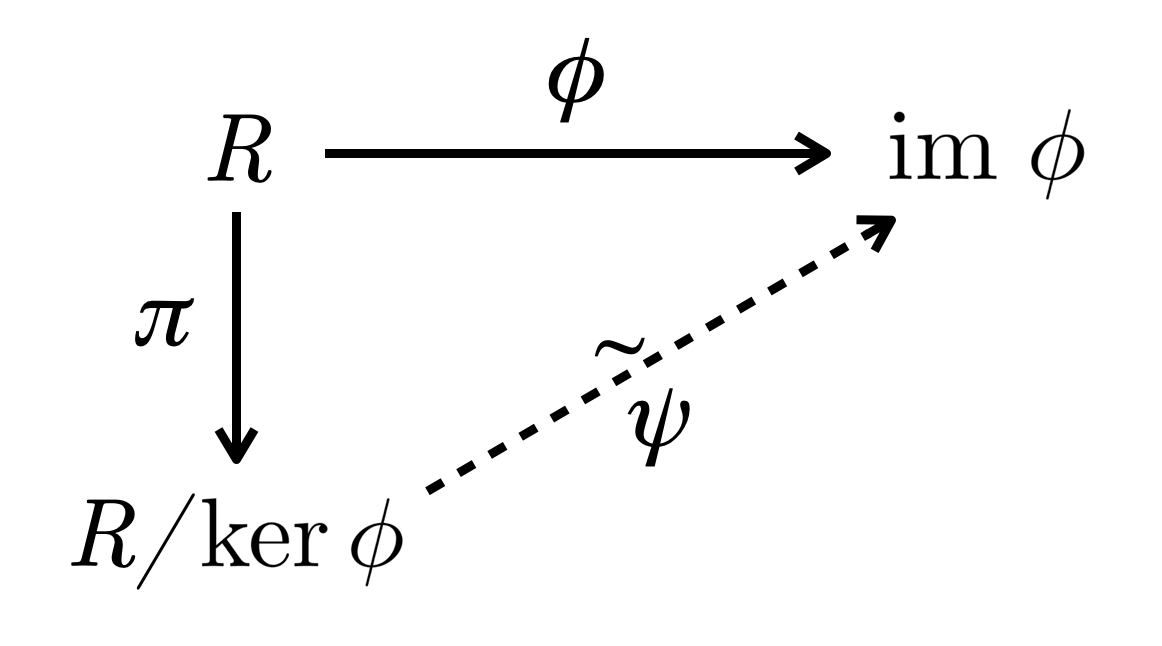
\includegraphics[width=0.35\textwidth]{further-homomorphisms/iso-1-comm-diagram.png}}
    \caption{Commutativity Diagram for \myreffigures{thrm-isomorphism-1}}
\end{figure}

In the diagram, $\phi$ sends elements from $G$ to $\im\phi$ and $\pi$ sends elements from $G$ to $G/\ker\phi$. Then the map $\psi$ is a unique map that sends elements from $G/\ker\phi$ to the image of $\phi$.

\begin{proof}
    We know by \myref{prop-image-is-subgroup-of-codomain} that $\im\phi \leq H$. Let $\psi: G/\ker\phi \to \im\phi$ such that $\psi(x\ker\phi) = \phi(x)$. We need to check that $\psi$ is a well-defined isomorphism.
    \begin{itemize}
        \item \textbf{Well-defined}: Suppose $x\ker\phi = y\ker\phi$ where $x, y \in G$. Then $xy^{-1} \in \ker\phi$ by Coset Equality (\myref{lemma-coset-equality}), statements 1 and 5. This means that $\phi(xy^{-1}) = e_H$ by definition of the kernel. Note $\phi(xy^{-1}) = \phi(x)\left(\phi(y)\right)^{-1}$, so $\phi(x)\left(\phi(y)\right)^{-1} = e_H$. Hence $\phi(x) = \phi(y)$. Thus,
        \[
            \psi(x\ker\phi) = \phi(x) = \phi(y) = \psi(y\ker\phi)
        \]
        so $\psi$ is well-defined.

        \item \textbf{Homomorphism}: Note that
        \begin{align*}
            \psi((x\ker\phi)(y\ker\phi)) &= \psi((xy)\ker\phi)\\
            &= \phi(xy)\\
            &= \phi(x)\phi(y)\\
            &= \psi(x\ker\phi)\psi(y\ker\phi)
        \end{align*}
        so $\psi$ is a homomorphism.
        \item \textbf{Injective}: By \myref{exercise-trivial-kernel-means-injective}, we check that $\psi$ is injective by showing that $\ker\psi$ is trivial, i.e. $\ker\psi = \{\ker\phi\}$.

        Suppose $x\ker\phi\in\ker\psi$. Then $\psi(x\ker\phi) = e_H$ by definition of kernel. Hence $\phi(x) = e_H$ by definition of $\psi$, which means $x \in \ker\phi$ by definition of kernel. Thus $x\ker\phi = \ker\phi$ by Element in Coset (\myref{corollary-equivalence-of-element-in-coset}). Therefore $\psi$ is injective.

        \item \textbf{Surjective}: Suppose $y$ is in the image of $\phi$, meaning there exists a $x \in G$ such that $\phi(x) = y$. Note that $\psi(x\ker\phi) = \phi(x) = y$. Thus $\psi$ is surjective.
    \end{itemize}
    Thus $\psi$ is a well-defined isomorphism.

    We now check that $\psi$ satisfies the requirement that $\psi\pi = \phi$. Let $x \in G$. Note that $\pi(x) = x\ker\phi$, and
    \[
        \psi\pi(x) = \psi(x\ker\phi) = \phi(x)
    \]
    for all $x \in G$, so $\psi\pi = \phi$.

    Finally we show that $\psi$ is unique. Suppose $f: G/\ker\phi \to \im\phi$ is an isomorphism satisfying $f\pi=\phi$. Take $x\ker\phi \in G/\ker\phi$. Note that
    \begin{align*}
        f(x\ker\phi) &= f(\pi(x))\\
        &= (f\pi)(x)\\
        &= \phi(x)\\
        &= (\psi\pi)(x)\\
        &= \psi(\pi(x))\\
        &= \psi(x\ker\phi)
    \end{align*}
    for all $x \in G$, meaning that $f = \psi$. Therefore $\psi$ is unique.

    Hence, $\psi$ is a unique isomorphism satisfying $\psi\pi = \phi$.
\end{proof}

\begin{example}
    Let $R = \{x \in \R \vert x > 0\}$, $G = \{x \in \R \vert x \neq 0\}$, and $H = \{1, -1\}$ be groups under multiplication. We show $G / H \cong R$.

    Consider the map $\phi: G \to R$ where $x \mapsto |x|$. We show that $\phi$ is a homomorphism, then find the image of $\phi$, and finally find its kernel.

    \begin{itemize}
        \item \textbf{Homomorphism}: $\phi$ is a homomorphism since $\phi(xy) = |xy| = |x||y| = \phi(x)\phi(y)$.
        \item \textbf{Image}: We find the image of $\phi$.
        \begin{align*}
            \im\phi &= \{\phi(x) \vert x \in G\}\\
            &= \{|x| \vert x \neq 0\}\\
            &= \{x \in \R \vert x > 0\} & (\text{by definition of } |x|)\\
            &= R
        \end{align*}
        which actually means that $\phi$ is surjective.
        \item \textbf{Kernel}: We find the kernel of $\phi$.
        \begin{align*}
            \ker\phi &= \{x \in G \vert \phi(x) = 1\} & (1 \text{ is the identity in } R)\\
            &= \{x \in G \vert |x| = 1\}\\
            &= \{1, -1\}\\
            &= H
        \end{align*}
    \end{itemize}
    Thus $G/H \cong R$ by the Fundamental Homomorphism Theorem (\myref{thrm-isomorphism-1}).
\end{example}

\begin{exercise}
    Let $\phi: G \to H$ be a homomorphism between finite groups $G$ and $H$. Prove that
    \[
        |G| = |\im \phi|\times|\ker \phi|.
    \]
\end{exercise}

\section{The Diamond Isomorphism Theorem}
We now look at the next theorem, called the \textbf{Diamond Isomorphism Theorem} (e.g. in {\cite[Theorem 3.18]{dummit_foote_2004}}) or the \textbf{Second Isomorphism Theorem} (e.g. in {\cite[\S 69]{clark_1984}}).
\begin{theorem}[Diamond Isomorphism Theorem]\label{thrm-isomorphism-2}\index{Diamond Isomorphism Theorem}\index{Isomorphism Theorem!Second}
    Let $G$ be a group and let $H$ and $K$ be subgroups of $G$. Then
    \begin{enumerate}
        \item $H \cap K \leq H$; and
        \item $H \leq HK$.
    \end{enumerate}
    Furthermore, if $N \unlhd G$, then
    \begin{enumerate}[start=3]
        \item $HN \leq G$;
        \item $H \cap N \unlhd H$;
        \item $N \unlhd HN$; and
        \item $H / (H\cap N) \cong HN / N$.
    \end{enumerate}
\end{theorem}

\newpage

We can capture the overall relationships of the subgroups of $G$ using a \textbf{subgroup lattice}.
\begin{figure}[h]
    \centering
    \fbox{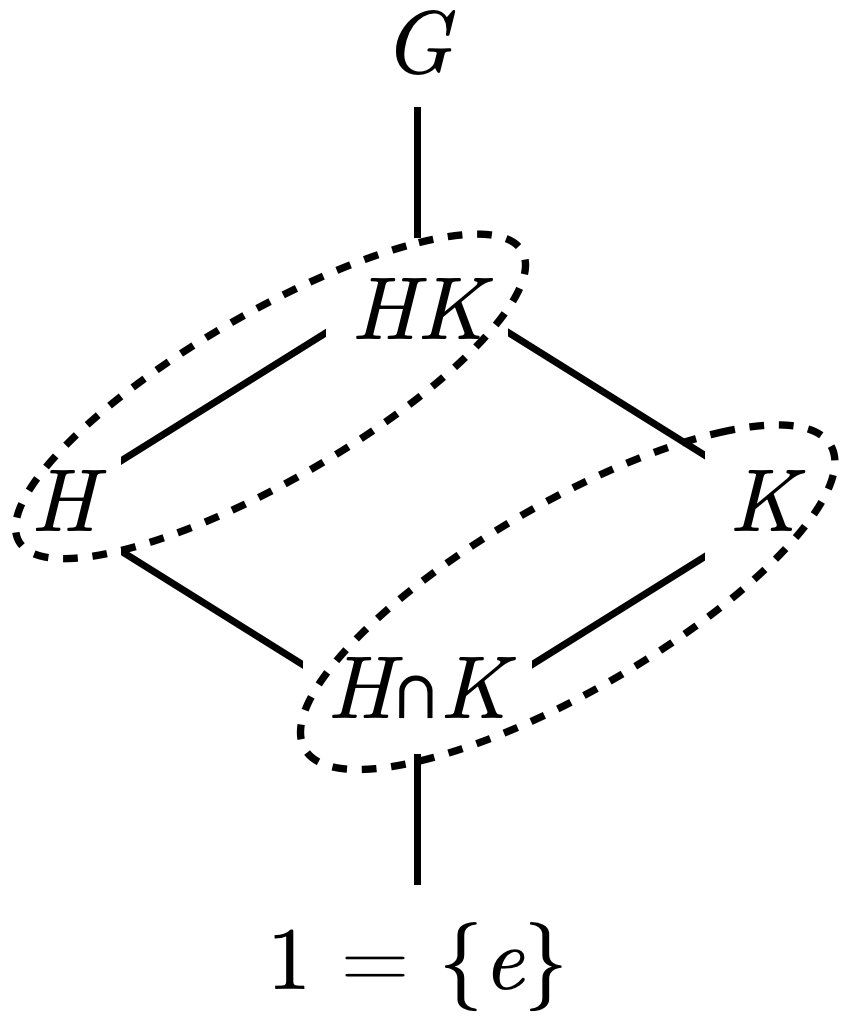
\includegraphics[width=0.25\textwidth]{further-homomorphisms/iso-2-subgroup-diagram.png}}
    \caption{Subgroup Lattice for \myreffigures{thrm-isomorphism-2}}
\end{figure}

We only show subgroups that we care about in the diagram. The group $G$ has a (direct) subgroup $HK$; $HK$ has subgroups $H$ and $K$; and $H$ and $K$ has a common subgroup $H\cap K$. The dotted quotient groups are isomorphic to each other if $H \unlhd G$.

\begin{proof}
    We prove each statement in sequence.

    \begin{enumerate}
        \item Clearly $e_G \in H$ and $e_G \in K$ so $e_G \in H \cap K$. Now take $x, y \in H \cap K$, meaning $x, y \in H$ and $x, y \in K$. Since $H, K \leq G$ so $xy^{-1} \in H$ and $xy^{-1} \in K$. Thus $xy^{-1} \in H \cap K$. By the subgroup test, this means that $H \cap K \leq H$.
        
        \item Note that $H = \{he_G \vert h \in H\} \subseteq \{hk \vert h \in H, k \in K\} = HK$, and $H$ is a group (as $H$ is a subgroup). Therefore $H \leq HK$.
        
        \item We note that, because $N$ is normal, hence $hN = Nh$ for all $h \in H \subseteq G$, meaning that $HN = NH$. Therefore by \myref{prop-subgroup-product-is-subgroup}, we have $HN \leq G$.

        \item We know $H \cap N \leq H$ by statement 1, so we only prove normality. Take $x \in H \cap N$. Since $H \leq G$, thus $x \in H \cap N \subseteq H$, meaning for all $g \in H$, $gxg^{-1} \in H$ (where we think of $g$ and $x$ as being in $H$). But since $x \in H \cap N \subseteq N$ and $N \unlhd G$, thus $gxg^{-1} \in N$ (where we think of $g \in H$ and $x \in N$). Therefore $H \cap N \unlhd H$.

        \item We know $N \leq HN$ by statement 2, so we only prove normality. Take $n \in N$ and $x \in HN$ such that $x = h_xn_x$. Then
        \begin{align*}
            xnx^{-1} &= (h_xn_x)n(h_xn_x)^{-1}\\
            &= (h_xn_x)n(n_x^{-1}h_x^{-1}) & (\text{Shoes and Socks})\\
            &= \underbrace{h_x}_{\text{In }G}\underbrace{n_xnn_x^{-1}}_{\text{In }N}\underbrace{h_x^{-1}}_{\text{In G}}\\
            &\in N
        \end{align*}
        since $N \unlhd G$. This proves that $N \unlhd HN$.

        \item This is the main result of this theorem. We define $\phi: H \to HN/N, h \mapsto hN$. We show that $\phi$ is a homomorphism and then find its image and kernel.
        \begin{itemize}
            \item \textbf{Homomorphism}:
            \[
                \phi(xy) = (xy)N = (xN)(yN) = \phi(x)\phi(y)    
            \]

            \item \textbf{Image}: We show that $\phi$ is surjective to show that $\im\phi = HN/N$. Suppose $x \in HN$, meaning $x = hn$ where $h \in H$ and $n \in N$. Thus $xN \in HN/N$, so
            \[
                xN = (hn)N = h(nN) = hN
            \]
            meaning $\phi(h) = hN = xN$. Hence we have found a pre-image of the coset $xN$, meaning $\phi$ is surjective. Thus $\im \phi = HN/N$.

            \item \textbf{Kernel}: We claim that $\ker\phi = H \cap N$.
            
            Note that $\ker\phi = \{h \in H \vert \phi(h) = eN = N\}$ by definition of kernel. This means that if $h \in \ker\phi$ then $\phi(h) = N$. Hence $\phi(h) = hN = N$, which means $h \in N$ by Element in Coset (\myref{corollary-equivalence-of-element-in-coset}). Thus, $h \in H$ and $h \in N$, meaning $h \in H \cap N$. Therefore $\ker \phi \subseteq H \cap N$.
    
            Now suppose $x \in H \cap N$. This means that $x \in N$ necessarily, implying $xN = N$. Thus $\phi(x) = N$ which quickly implies $x \in \ker\phi$. Therefore $H \cap N \subseteq \ker\phi$.
    
            Since $\ker \phi \subseteq H \cap N$ and  $H \cap N \subseteq \ker\phi$ therefore $\ker\phi = H\cap N$.
        \end{itemize}

        By the Fundamental Homomorphism Theorem (\myref{thrm-isomorphism-1}),
        \[
            H / \ker\phi \cong \im \phi,
        \]
        which means
        \[
            H/(H\cap N) \cong HN/N.
        \]
    \end{enumerate}
    This completes the proof of the theorem.
\end{proof}

\begin{corollary}\label{corollary-subgroup-product-is-normal-subgroup-if-subgroups-are-normal}
    Let $G$ be a group with proper subgroups $H$ and $K$. Then $HK \unlhd G$ if $H$ and $K$ are normal subgroups of $G$.
\end{corollary}
\begin{proof}
    Assume that $H, K \lhd G$. By the Diamond Isomorphism Theorem (\myref{thrm-isomorphism-2}), statement 3, we know that $HK \leq G$ since $H \lhd G$. We just need to prove normality. Suppose $hk \in HK$ and take $g \in G$. Then
    \begin{align*}
        g(hk)g^{-1} &= (gh)(kg^{-1})\\
        &= (hg)(g^{-1}k) & (\text{as } H, K \lhd G)\\
        &= h(gg^{-1})k\\
        &= hk \in HK
    \end{align*}
    which means that $HK \unlhd G$.
\end{proof}

We look at two examples using the Diamond Isomorphism Theorem.
\begin{example}
    We say a group $G$ is \textbf{metabelian}\index{metabelian} if and only if there exists $A \unlhd G$ such that $A$ and $G/A$ are both abelian. We will prove that any subgroup of a metabelian group is also metabelian.

    Let $H \leq G$. Then, by the Diamond Isomorphism Theorem (\myref{thrm-isomorphism-2}), we know $H \cap A \unlhd H$ (statement 4) and $H/(H \cap A) \cong HA / A$ (statement 6). We just need to prove that both $H \cap A$ and $H/(H \cap A)$ are abelian.
    \begin{itemize}
        \item Consider any two elements from $H \cap A$, say $x$ and $y$. Then $x \in A$ and $y \in A$, so $xy = yx$ as $A$ is abelian. Hence, elements from $H \cap A$ commute, meaning that $H \cap A$ is abelian.
        \item Consider $H/(H\cap A) \cong HA / A$. Note that $HA \leq G$ since $H \leq G$ and $A \leq G$. Thus, $HA / A \leq G / A$. Note that $G/A$ is abelian by definition of metabelian group. Hence, $H/(H \cap A)$ is also abelian.
    \end{itemize}
    Therefore, we have found a subgroup of $H$ (in particular $H \cap A$) such that both $H \cap A$ and $H/(H\cap A)$ are both abelian. Hence, $H$ is metabelian.
\end{example}

We look at another application of the Diamond Isomorphism Theorem, which has use in Number Theory.
\begin{example}
    We will prove that $\lcm(m,n)\times\gcd(m,n) = mn$ (\myref{prop-product-of-gcd-and-lcm}) by considering the Diamond Isomorphism Theorem. For brevity, let $d = \gcd(m,n)$ and $l = \lcm(m,n)$.

    Consider the groups $G = \Z$, $H = m\Z$, and $N = n\Z$ under addition. By Diamond Isomorphism Theorem (\myref{thrm-isomorphism-2}),
    \[
        m\Z/(m\Z \cap n\Z) \cong (m\Z + n\Z)/(n\Z).
    \]

    Now $m\Z \cap n\Z$ is the set of integers that are both a multiple of $m$ and $n$. Hence, $m\Z \cap n\Z = \lcm(m,n)\Z = l\Z$. On the other hand, $m\Z + n\Z$ is the set of all integers of the form $mx+ny$ where $x$ and $y$ are integers. B\'{e}zout's lemma (\myref{lemma-bezout}) tells us that this set consists of the multiples of $\gcd(m,n)$, i.e. $m\Z + n\Z = \gcd(m,n)\Z = d\Z$. Hence,
    \[
        m\Z/(l\Z) \cong d\Z/(n\Z).
    \]

    We claim that $m\Z / (l\Z) \cong \Z_{\frac lm} \text{ and } d\Z / (n\Z) \cong \Z_{\frac nd}$. This is a specific case of \myref{problem-mZ/nZ-isomorphic-to-Zn/m} which we have left as a problem for later. Hence,
    \[
    \Z_{\frac lm} \cong m\Z/(l\Z) \cong d\Z/(n\Z) \cong \Z_{\frac nd},
    \]
    which means that $\Z_{\frac lm} \cong \Z_{\frac nd}$. We can now finally take orders on both sides:
    \[
        \frac{l}{m} = \frac{n}{d},
    \]
    which means that $ld = mn$. Hence, $\lcm(m,n)\times\gcd(m,n) = mn$.
\end{example}

\begin{exercise}\label{exercise-order-of-subgroup-product}
    Let $G$ be a finite group, $H \leq G$, and $N \lhd G$. Prove that
    \[
        |HN| = \frac{|H||N|}{|H \cap N|}.
    \]
\end{exercise}

\section{The Third Isomorphism Theorem}
We look at the last important theorem regarding homomorphisms and isomorphisms. This is often called the \textbf{Third Isomorphism Theorem} (e.g. in {\cite[Corollary I.5.10]{hungerford_1980}} and {\cite[pp.~253--254, Theorem 5]{cohn_1982}}).

It should be noted that there is no consistency with the numbering of these theorems in books (cf. {\cite[\S 68]{clark_1984}} as ``First Isomorphism Theorem'', {\cite[Theorem 8.16]{humphreys_1996}} as ``Second Isomorphism Theorem''), but the name ``Third Isomorphism Theorem'' is the easiest to research. Hence, we use that name here.

\begin{theorem}[Third Isomorphism Theorem]\label{thrm-isomorphism-3}\index{Isomorphism Theorem!Third}
    Let $G$ be a group. Let $H \unlhd G$ and $N \unlhd G$. Suppose $N \subseteq H$. Then
    \begin{enumerate}
        \item $N \unlhd H$;
        \item $H/N \unlhd G/N$; and
        \item $\frac{G/N}{H/N} \cong G/H$.
    \end{enumerate}
\end{theorem}
\begin{proof}
    We prove the statements in sequence.

    \begin{enumerate}
        \item We note that since $N \subseteq H$ and $N$ is a group (since $N$ is a normal subgroup of $G$) thus $N \leq H$. We just need to prove normality. Since $H$ and $N$ are normal subgroups of $G$, thus for all $g \in G$,
        \[
            gH = Hg \text{ and } gN = Ng.
        \]
        Now since $N \subseteq H \subseteq G$, thus for all $n$ in $N$, $nH = Hn$ (since $n \in G$). This means that $N \unlhd H$.

        \item We first prove that it is a subgroup before proving normality.

        Clearly $N = eN \in H/N$. Let $x$ and $y$ be in $H/N$. Then $x=h_xN$ and $y=h_yN$ for some $h_x, h_y \in H$. Note that $y^{-1} = (h_y^{-1})N$ by group operator on cosets. Hence,
        \begin{align*}
            xy^{-1} &= (h_xN)(h_y^{-1}N)\\
            &= (\underbrace{h_xh_y^{-1}}_{\text{In }H})N\\
            &\in H/N
        \end{align*}
        Hence, by subgroup test, $H/N \leq G/N$.

        Now let $gN \in G/N$ and $hN \in H/N$. We need to show that $(gN)(hN)(gN)^{-1} \in H/N$. Note $(gN)(hN)(gN)^{-1} = (ghg^{-1})N$. Since $H \unlhd G$, thus $ghg^{-1} \in H$ which means that $(ghg^{-1})N \in H/N$.

        Therefore $H/N \unlhd G/N$.

        \item This is the main result of the theorem.

        Define $\phi: G/N \to G/H, gN \mapsto gH$. We check that $\phi$ is a well-defined homomorphism and find its image and kernel.
        \begin{itemize}
            \item \textbf{Well-defined}: Suppose $gN = g'N$. Then $g(g')^{-1} \in N$ by Coset Equality (\myref{lemma-coset-equality}), statements 1 and 5. Since $N \subseteq H$, thus $g(g')^{-1} \in H$ which implies $gH = g'H$, again by Coset Equality, statements 1 and 5. Hence
            \[
                \phi(gN) = gH = g'H = \phi(g'N)
            \]
            so $\phi$ is well-defined.

            \item \textbf{Homomorphism}: Take $gN, g'N \in G/N$. Then
            \begin{align*}
                \phi((gN)(g'N)) &= \phi((gg')N)\\
                &= (gg')H\\
                &= (gH)(g'H)\\
                &= \phi(gN)\phi(g'N)
            \end{align*}
            which means that $\phi$ is a homomorphism.
            
            \item \textbf{Image}: We show $\phi$ is surjective to prove that $\im\phi = G/H$. Suppose $gH \in G/H$. Clearly $\phi(gN) = gH$. Thus $gN$ is a pre-image of $gH$, meaning that $\phi$ is surjective. Hence $\im\phi = G/H$.
            
            \item \textbf{Kernel}: Suppose $gN \in \ker\phi = \{gN \vert \phi(gN) = eH = H\}$. Thus $\phi(gN) = gH = H$, which means $g \in H$. Hence $gN \in H/N$, so $\ker\phi \subseteq H/N$.

            Now assume $hN \in H/N$. Since $H\subseteq G$ (as $H \unlhd G$), thus $h \in G$. Therefore $hN \in G/N$, so $\phi(hN) = hH = H$. Hence $hN \in \ker\phi$ which means $H/N \subseteq \ker\phi$.

            Since $\ker\phi \subseteq H/N$ and $H/N \subseteq \ker\phi$, we must have $\ker\phi = H/N$.
        \end{itemize}

        By the Fundamental Homomorphism Theorem (\myref{thrm-isomorphism-1}), we have $\frac{G/N}{\ker\phi} \cong \im\phi$, which means
        \[
            \frac{G/N}{H/N} \cong G/H,
        \]
        proving statement 3.
    \end{enumerate}
    This proves the theorem.
\end{proof}

\begin{example}
    Take $G = \Z$, $H = m\Z$, and $N = mn\Z$. Note that clearly $H, N \leq G$, and since $G$ is abelian, we must also have $H \unlhd G$ and $N \unlhd G$. By the Third Isomorphism Theorem (\myref{thrm-isomorphism-3}), statement 3,
    \[
        \frac{G/N}{H/N} \cong G/H.
    \]
    Note $G/H = \Z/(m\Z) \cong \Z_m$ by \myref{problem-Zn-isomorphic-to-Z-by-nZ}. Note also
    \[
        \frac{G/N}{H/N} = \frac{\Z/(mn\Z)}{m\Z/(mn\Z)}.
    \]
    Hence we see that
    \[
        \frac{\Z/(mn\Z)}{m\Z/(mn\Z)} \cong \Z/(m\Z) \cong \Z_m.
    \]
\end{example}

\begin{exercise}
    Suppose $x$ and $y$ are positive integers such that $y = mx$ for some integer $m$. Let $H = x\Z$ and $N = y\Z$ be groups under addition.
    \begin{partquestions}{\roman*}
        \item Explain why $N \subseteq H$.
        \item Find a group $G$ such that $H \lhd G$ and $N \lhd G$.
        \item Hence find the order of $H/N$.
    \end{partquestions}
\end{exercise}

\newpage

\section{Problems}
\begin{problem}
    Let $G$ be a group. Prove that $G/G$ is isomorphic to the trivial group.
\end{problem}

\begin{problem}
    Let $R = (\R, +)$. Also let $G = R^2$ and $H = \left\{(r\sqrt2, r\sqrt3) \vert r\in R\right\}$ be groups under component-wise addition. Prove that $G/H \cong R$.
\end{problem}

\begin{problem}\label{problem-subgroup-product-equal-to-subgroup-if-one-is-subgroup-of-another}
    Let $G$ be a group. Let $H$ and $K$ be subgroups of $G$ such that $K \subseteq H$. Prove that $HK = H$.
\end{problem}

\begin{problem}\label{problem-cartesian-product-of-group-by-group-isomorphic-to-group}
    Let $G$ be an abelian group with operation $\ast$. Let $I = \{(g, g^{-1}) \vert g \in G\}$ be a group under component-wise application of $\ast$.
    \begin{partquestions}{\roman*}
        \item Show that $I \cong G$.
        \item Hence prove $G^2/G \cong G$ by considering a suitable homomorphism.
    \end{partquestions}
\end{problem}

\begin{problem}\label{problem-mZ/nZ-isomorphic-to-Zn/m}
    Let $G = m\Z$ and $H = n\Z$ be groups under addition, where $m\vert n$ and $m \neq n$. Let the map $\phi: G \to \Z/({\frac nm}\Z)$ be defined such that
    \[
        \phi(am) = a + \frac nm \Z.
    \]
    Prove that $G/H \cong \Z_{\frac nm}$.
\end{problem}

\chapter{More Types of Groups}
We previously introduced some types of groups, like the cyclic groups, the dihedral groups, and the Klein-four group. We now introduce more types of groups to expand our knowledge of the types of groups that are involved in group theory.

\section{More About Cyclic Groups}
We previously covered several properties of cyclic groups.
\begin{itemize}
    \item Every cyclic group is abelian. (\myref{prop-cyclic-group-is-abelian})
    \item A finite group $G$ is cyclic if and only if there exists an element $g$ in the group $G$ with the same order as the group. (\myref{thrm-cyclic-group-has-element-with-same-order})
    \item If $G$ is cyclic and $H \leq G$ then $G/H$ is cyclic. (\myref{exercise-quotient-group-of-cyclic-group-is-cyclic})
    \item Any subgroup of a cyclic group is cyclic. (\myref{problem-subgroup-of-cyclic-group-is-cyclic})
    \item $\Z / (n\Z) \cong \Z_n$. (\myref{problem-Zn-isomorphic-to-Z-by-nZ})
    \item $\Z_m \times \Z_n \cong \Z_{mn}$ if and only if $\gcd(m,n) = 1$. (\myref{thrm-Zm-cross-Zn-isomorphic-to-Zmn-condition})
    \item $m\Z / n\Z \cong \Z_{\frac nm}$. (\myref{problem-mZ/nZ-isomorphic-to-Zn/m})
\end{itemize}

\begin{exercise}\label{exercise-Zmn-mod-Zn-cong-Zn}
    Prove that
    \[
        \Z_{mn} / \Z_m \cong \Z_n.
    \]
    for any positive integers $m$ and $n$.
\end{exercise}

Note that we may denote the finite cyclic group of order $n$ by $\Cn{n}$ instead of $\Z_n$. This may be sometimes used to distinguish (finite) cyclic subgroups of a group from the integers modulo $n$.

We prove an essential theorem on cyclic groups. Before that, we require the following lemma.
\begin{lemma}\label{lemma-order-of-an-element-that-is-equivalent-to-identity}
    Let $\Cn{n}$ have generator $g$. Then $g^k = e$ if and only if $k$ is a multiple of $n$.\newline
    (That is, if $g^k = e$ then $n$ divides $k$, i.e. $n\vert k$.)
\end{lemma}
\begin{proof}
    We note that the order of $g$ is $n$, since $g$ is a generator of $G$. Thus by \myref{problem-element-to-power-of-multiple-of-order-is-identity} the lemma is proven.
\end{proof}

\newpage

\begin{theorem}\label{thrm-order-of-element-in-cyclic-group}
    Let $\Cn{n}$ have generator $g$. Let $x = g^k$ for some integer $k$. Then
    \[
        |x| = \frac{n}{\gcd(k,n)}.
    \]
\end{theorem}
\begin{proof}
    For brevity let $m = |x|$ and suppose $k = \lambda \gcd(k, n)$ for some positive integer $\lambda$.

    Let $\mathcal{X} = \langle x \rangle = \{x, x^2, x^3, \dots, x^m\}$. Note that $\mathcal{X}$ is a cyclic group with order $m$ and generator $x$.

    Observe that
    \[
        x^m = \left(g^k\right)^m = g^{km}
    \]
    and since $|x| = m$, this means that $x^m = e$. Hence $g^{km} = e$. By \myref{lemma-order-of-an-element-that-is-equivalent-to-identity} on $\Cn{n}$, $n \vert km$. This implies that
    \[
        \frac{n}{\gcd(k,n)} \vert \frac{km}{\gcd(k,m)} = \lambda m.
    \]
    Note that $\gcd\left(\lambda, \frac{n}{\gcd(k,n)}\right) = \gcd\left(\frac{k}{\gcd(k,n)}, \frac{n}{\gcd(k,n)}\right) = 1$. This means that $\frac{n}{\gcd(k,n)}$ does not divide $\lambda$, meaning $\frac{n}{\gcd(k,n)} \vert m$.

    Also note that
    \begin{align*}
        x^{\frac{n}{\gcd(k,n)}} &= \left(g^k\right)^{\frac{n}{\gcd(k,n)}}\\
        &= \left(g^n\right)^{\frac{k}{\gcd(k,n)}}\\
        &= \left(g^n\right)^\lambda\\
        &= e^\lambda & (\text{since } |g| = n)\\
        &= e,
    \end{align*}
    implying $x^{\frac{n}{\gcd(k,n)}} = e$. By \myref{lemma-order-of-an-element-that-is-equivalent-to-identity} on group $\mathcal{X}$, we have $m \vert \frac{n}{\gcd(k,n)}$.

    Since $\frac{n}{\gcd(k,n)} \vert m$ and $m \vert \frac{n}{\gcd(k,n)}$ simultaneously, thus $m = \frac{n}{\gcd(k,n)}$, that is,
    \[
        |x| = \frac{n}{\gcd(k,n)}.\qedhere
    \]
\end{proof}

\begin{exercise}
    The number 12 is equivalent to 0 in the group $\Z_n$. What are the possible value(s) of $n$?
\end{exercise}
\begin{exercise}
    In the group $\Z_{210}$, find the order of 10, 42, 75, and 140.
\end{exercise}

\begin{corollary}\label{corollary-element-in-cyclic-group-is-generator-iff-gcd-is-1}
    Let $\Cn{n}$ have generator $g$. Then $g^m$ is also a generator if and only if $\gcd(m, n) = 1$.
\end{corollary}
\begin{proof}
    We prove the forward direction first. Suppose that $\Cn{n}$ has a generator of $g^m$. On one hand, $|g^m| = n$ since a generator of a group necessarily has to have an order equal to that of the group. On another hand, by \myref{thrm-order-of-element-in-cyclic-group}, $|g^m| = \frac{n}{\gcd(m, n)}$. Hence, $n = \frac{n}{\gcd(m, n)}$ which quickly implies $\gcd(m, n) = 1$.

    Now we prove the reverse direction. Suppose $\gcd(m,n) = 1$. Then $|g^m| = \frac{n}{\gcd(m,n)} = \frac{n}{1} = n$ by \myref{thrm-order-of-element-in-cyclic-group}. Hence $g^m$ is a generator of $\Cn{n}$ by \myref{thrm-cyclic-group-has-element-with-same-order}.
\end{proof}

\begin{exercise}
    Find all the generators of the following groups.
    \begin{partquestions}{\alph*}
        \item $\Z_{10}$
        \item $\Z_{101}$
    \end{partquestions}
\end{exercise}

\section{Quaternion Group}
We look at an interesting group that has use in computer graphics: the \textbf{quaternion group}. We present one definition here.
\begin{definition}\label{definition-quaternion-group}
    The quaternion group\index{quaternion group} is
    \[
            \mathrm{Q} = \{1, -1, i, -i, j, -j, k, -k\}
    \]
    where
    \begin{multicols}{2}
        \begin{itemize}
            \item 1 is the identity;
            \item $(-1)^2 = 1$;
            \item $i^2 = j^2 = k^2 = -1$;
            \item $ij = k$ and $ji = -k$;
            \item $jk = i$ and $kj = -i$; and
            \item $ki = j$ and $ik = -j$.
        \end{itemize}
    \end{multicols}
\end{definition}

The quaternion group has 4 proper non-trivial subgroups, namely $\langle -1 \rangle = \{\pm1\}$, $\langle i \rangle = \{\pm1, \pm i\}$, $\langle j \rangle = \{\pm1, \pm j\}$, and $\langle k \rangle = \{\pm1, \pm k\}$.

With these subgroups, we can write a presentation for $\mathrm{Q}$.
\begin{proposition}
    $\mathrm{Q} = \langle i, j \rangle$.
\end{proposition}
\begin{proof}
    For brevity let $G = \langle i, j \rangle$. We note that $i^0 = 1$, $i^4 = j^4 = 1$ and $ji = -k = -ij = i^3j$. Hence,
    \begin{align*}
        G &= \{1, i, i^2, i^3, j, ij, i^2j, i^3j\}\\
        &= \{1, i, -1, -i, j, ij, -j, -ij\}\\
        &= \{1, -1, i, -i, j, -j, ij, -ij\} & (\text{reordering})\\
        &= \{1, -1, i, -i, j, -j, k, -k\} & (\text{since } ij = k)\\
        &= \mathrm{Q}
    \end{align*}
    so $\mathrm{Q} = \langle i, j \rangle$.
\end{proof}

Thus, an alternate definition of $\mathrm{Q}$ is
\[
    \mathrm{Q} = \langle \alpha, \beta \vert \alpha^4 = e,\; \alpha^2 = \beta^2, \text{ and } \beta\alpha = \alpha^3\beta \rangle.
\]
One sees clearly that $\alpha = i$ and $\beta = j$ in this definition.

\begin{exercise}\label{exercise-normal-subgroups-of-quarternion-group}
    Find all the normal subgroups of the quaternion group $\mathrm{Q}$.\newline
    (\textit{Hint: consider \myref{problem-subgroup-of-index-2}.})
\end{exercise}

\section{Alternating Group}
The alternating group is a very important group in the field of group theory. However, before we can properly define it, we need to introduce the idea of \textbf{transpositions}.

\subsection{Transpositions}
\begin{definition}
    A \textbf{transposition}\index{transposition} is a 2-cycle. That is, a transposition $\tau$ is represented as $(a\quad b)$ in cycle notation.
\end{definition}
For example, we see that (1 5), (4 7), (3 6) etc. are transpositions, while (1 4 5), (3 4 6 5 9), (1 3 4 5) etc. are not. One sees clearly that every transposition is its own inverse.

We call transpositions which has cycle decomposition $\begin{pmatrix}i&i+1\end{pmatrix}$ \textbf{adjacent transpositions}\index{transposition!adjacent}, and we may denote them by $\alpha$.

We look at one lemma which can be said to help `break up' transpositions into a composition of adjacent transpositions. Ignore line breaks in the following lemma.
\begin{lemma}\label{lemma-decompose-transposition}
    Let a transposition $\tau = (i\quad i+d)$ where $d$ is a positive integer. Then $\tau$ is equal to the permutation
    \begin{align*}
        & (i\quad i+1)(i+1\quad i+2)\cdots(i+d-2\quad i+d-1)(i+d-1\quad i+d)\\
        &\quad (i+d-2\quad i+d-1)\cdots(i+1\quad i+2)(i\quad i+1)
    \end{align*}
\end{lemma}

\begin{proof}
    We induct on $d$.

    When $d = 1$, note $\tau = (i\quad i+1)$ so the lemma is true for $d=1$.

    Assume that the given representation of $\tau$ holds for some positive integer $d$. Note this means that it holds for all $i$, including $i+1$. We are to show that it works for $d + 1$.
    \begin{align*}
        (i\quad i+(d+1)) &= (i\quad i+1)(i+1\quad i+d+1)(i\quad i+1)\\
        &= (i\quad i+1)\underbrace{((i+1)\quad (i+d)+1)}_{\text{use induction hypothesis here}}(i\quad i+1)\\
        &= (i\quad i+1)((i+1)\quad(i+1)+1)\cdots((i+1)\quad(i+1)+1)(i\quad i+1)\\
        &= (i\quad i+1)(i+1\quad i+2)\cdots(i+1\quad i+2)(i\quad i+1)
    \end{align*}
    which shows that $d+1$ works as well.
\end{proof}
\begin{remark}
    The above representation of $\tau$ uses $2d-1$ compositions.
\end{remark}
\begin{example}
    An adjacent transposition decomposition of $(4\quad9)$ is
    \[
        (4\quad 5)(5\quad 6)(6\quad 7)(7\quad 8)(8\quad 9)(7\quad 8)(6\quad 7)(5\quad 6)(4\quad 5).
    \]
\end{example}
\begin{exercise}
    `Decompose' the transposition (2 6) into a composition of adjacent transpositions.
\end{exercise}

\subsection{Links with Permutations}
As mentioned before, a transposition is a 2-cycle permutation. We note that transpositions are important as seen in the following lemma.
\begin{lemma}\label{lemma-permutations-as-product-of-transpositions}
    Every permutation can be expressed as a product of transpositions.
\end{lemma}
\begin{proof}[Proof (see {\cite[\S 80 Corollary]{clark_1984}})]
    For the identity $\id$ it can be expressed as $(a\quad b)(a \quad b)$. For any permutation with length $k \geq 2$, say $\sigma = \begin{pmatrix}a_1 & a_2 & a_3 & \cdots & a_k\end{pmatrix}$, write
    \[
        \sigma = \begin{pmatrix}a_1 & a_k\end{pmatrix}\begin{pmatrix}a_1 & a_{k-1}\end{pmatrix}\begin{pmatrix}a_1 & a_{k-2}\end{pmatrix}\cdots\begin{pmatrix}a_1 & a_3\end{pmatrix}\begin{pmatrix}a_1 & a_2\end{pmatrix}
    \]
    and since every permutation is a product of cycles, thus every permutation is a product of transpositions.
\end{proof}

We now look at the idea of \textbf{inversions} inside permutations.
\begin{definition}
    Let $\sigma$ be a permutation. An \textbf{inversion}\index{permutation!inversion} of $\sigma$ between $i$ and $j$ exists if $i > j$ and $\sigma(i) < \sigma(j)$.
\end{definition}
An inversion between the elements $i$ and $j$ is denoted by either $(i, j)$ or $(\sigma(i), \sigma(j))$.
\begin{example}
    In the permutation $\sigma = \begin{pmatrix}1 & 3 & 2 & 4\end{pmatrix}$, we see that $3 \mapsto 2$ but $2 \mapsto 4$. Thus there is an inversion (3, 2) = (2, 4).
\end{example}

We now define the idea of \textbf{even} permutations and \textbf{odd} permutations.
\begin{definition}
    A permutation $\sigma$ is said to be \textbf{even}\index{permutation!even} if there are an even number of inversions in $\sigma$. If $\sigma$ is not even then it is said to be \textbf{odd}\index{permutation!odd}. The evenness or oddness of a permutation $\sigma$ is called the \textbf{parity of $\sigma$}\index{permutation!parity}.
\end{definition}

Counting the number of inversions in a permutation may be hard to do, so we have an alternative definition for the parity of a permutation.

\begin{theorem}\label{thrm-parity-of-permutation}
    Let $\sigma$ be a permutation. Suppose $\sigma$ can be expressed as a product of $n$ transpositions. Then $\sigma$ is even if and only if $n$ is even.
\end{theorem}
\begin{proof}
    We only need to show that the parity of $n$ and the parity of the permutation is the same to prove this.

    By \myref{lemma-permutations-as-product-of-transpositions}, all permutations can be produced by a sequence of transpositions, say $\sigma = \tau_1\tau_2\tau_3\cdots\tau_k$. By \myref{lemma-decompose-transposition}, every transposition can be written as a product of $2d - 1$ adjacent transpositions. Expressing each $\tau_i$ as a product of adjacent transpositions yields
    \[
        \sigma = \alpha_1\alpha_2\cdots\alpha_m
    \]
    where $\alpha_i$ is an adjacent transposition for $1 \leq i \leq m$. Note that the parity of $m$ is the same as that of $k$.

    It is clear that for any permutation $\pi$ and adjacent permutation $\alpha$, the permutation $\alpha\pi$ has either one more or one less inversion than $\pi$. Thus the parity of the number of inversions of a permutation is switched when composed with adjacent transpositions.

    We note that the identity permutation $\id$ is an even permutation. So $\alpha_1$ is odd, $\alpha_1\alpha_2$ is even, $\alpha_1\alpha_2\alpha_3$ is odd, etc., so $\alpha_1\alpha_2\cdots\alpha_m$ has the parity of $m$. Therefore the parity of the number of inversions of $\sigma$ is the parity of $k$ (since $m$ and $k$ have the same parity).
\end{proof}

\begin{corollary}\label{corollary-permutation-and-inverse-have-same-parity}
    $\sigma$ and $\sigma^{-1}$ have the same parity for any permutation $\sigma$.
\end{corollary}
\begin{proof}
    One observes clearly that $\sigma\sigma^{-1} = \id$. Since $\id$ is even, thus $\sigma\sigma^{-1}$ must be composed of an even number of transpositions (\myref{thrm-parity-of-permutation}).
    \begin{itemize}
        \item If $\sigma$ is even, then $\sigma$ can be expressed as a product of an even number of transpositions. Hence $\sigma^{-1}$ must also be a product of an even number of transpositions in order for $\sigma\sigma^{-1} = \id$ to be even.
        \item If $\sigma$ is odd, then $\sigma$ can be expressed as a product of an odd number of transpositions. Hence $\sigma^{-1}$ must also be a product of an odd number of transpositions in order for $\sigma\sigma^{-1} = \id$ to be even.
    \end{itemize}
    This proves the claim.
\end{proof}

We look at one final useful construct: the sign of a permutation.
\begin{definition}
    The \textbf{sign of a permutation}\index{permutation!sign} is $+1$ if the permutation is even and $-1$ if the permutation is odd.
\end{definition}
If $\sigma$ is the permutation, $N(\sigma)$ is the number of inversions in $\sigma$, and $m$ is the number of transpositions in the decomposition of $\sigma$, then the sign of $\sigma$ is given by the \textbf{signum} function:
\[
    \sgn(\sigma) = (-1)^{N(\sigma)} = (-1)^m.
\]
\begin{exercise}
    Find $\sgn\left(\begin{pmatrix}1&3&2&5&4\end{pmatrix}\right)$.
\end{exercise}

One observes that the number of inversions in $\sigma\tau$ is the same as the sum of inversions in $\sigma$ and $\tau$ separately, which means
\[
    N(\sigma\tau) = N(\sigma) + N(\tau)
\]
so
\begin{align*}
    \sgn(\sigma\tau) &= (-1)^{N(\sigma\tau)}\\
    &= (-1)^{N(\sigma) + N(\tau)}\\
    &= (-1)^{N(\sigma)}(-1)^{N(\tau)}\\
    &= \sgn(\sigma)\sgn(\tau),
\end{align*}
meaning that $\sgn$ is a \textit{multiplicative map}. One can then quickly verify \myref{corollary-permutation-and-inverse-have-same-parity} by noting
\[
    1 = \sgn(\id) = \sgn(\sigma\sigma^{-1}) = \sgn(\sigma)\sgn(\sigma^{-1})
\]
which implies $\sgn(\sigma)$ and $\sgn(\sigma^{-1})$ have the same parity.

\subsection{The Alternating Group}
We are now ready to look at the alternating group.
\begin{definition}
    The \textbf{alternating group of degree $n$}\index{alternating group!of degree $n$}, denoted by $\An{n}$, is given by
    \[
        \An{n} = \left\{\sigma \in \Sn{n} \vert \sigma \text{ is even}\right\}
    \]
    for $n \geq 2$.
\end{definition}

\begin{proposition}\label{prop-An-normal-subgroup-of-Sn}
    $\An{n} \lhd \Sn{n}$ where $n \geq 2$.
\end{proposition}
\begin{proof}
    Note that the identity function $\id \in \An{n}$ since $\id \in \Sn{n}$ and the identity is even.

    Suppose now that $\mu$ and $\sigma$ are in $\An{n}$. We show that $\mu\sigma^{-1} \in \An{n}$. By \myref{lemma-permutations-as-product-of-transpositions}, we may write
    \[
        \mu = \tau_1\tau_2\cdots\tau_{2k} \text{ and } \sigma = \tau_1'\tau_2'\cdots\tau_{2m}'.
    \]
    We note that any transposition is its own inverse, that is $\tau = \tau^{-1}$. Hence $\sigma^{-1} = \tau_{2m}'\tau_{2m-1}'\cdots\tau_2'\tau_1'$, so
    \[
        \mu\sigma^{-1} = \underbrace{\tau_1\cdots\tau_{2k}\tau_{2m}'\cdots\tau_1'}_{2(k+m) \text{ transpositions}}
    \]
    is an even permutation, meaning $\mu\sigma^{-1} \in \An{n}$. By subgroup test, $\An{n} \leq \Sn{n}$. But as $\An{n}$ contains only even permutations, thus $\An{n} < \Sn{n}$.
    
    Now take $\sigma \in \Sn{n}$ and $\mu \in \An{n}$. Note that
    \begin{align*}
        \sgn(\sigma\mu\sigma^{-1}) &= \sgn(\sigma)\sgn(\mu)\sgn(\sigma^{-1})\\
        &= \sgn(\sigma)\sgn(\sigma^{-1})\sgn(\mu)\\
        &= \sgn(\sigma\sigma^{-1})\sgn(\mu)\\
        &= \sgn(\id)\sgn(\mu)\\
        &= \sgn(\mu).
    \end{align*}
    \[
        \sgn(\sigma\mu\sigma^{-1}) = \sgn(\sigma)\sgn(\mu)\sgn(\sigma^{-1}).
    \]
    As $\mu$ is even, so $\sgn(\mu) = 1$. Hence $\sgn(\sigma\mu\sigma^{-1}) = 1$ which means that $\sigma\mu\sigma^{-1}$ is an even permutation. Therefore $\sigma\mu\sigma^{-1} \in \An{n}$, meaning that $\An{n} \lhd \Sn{n}$.
\end{proof}

\begin{proposition}\label{prop-order-of-An}
    The order of $\An{n}$ is $\frac{n!}{2}$ for $n \geq 2$.
\end{proposition}
\begin{proof}
    For brevity, let
    \[
        \mathrm{O}_n = \left\{\sigma \in \Sn{n} \vert \sigma \text{ is odd}\right\} = \Sn{n} \setminus \An{n}.
    \]
    Clearly $A_n \cup \mathrm{O}_n = \Sn{n}$ and $A_n \cap \mathrm{O}_n = \emptyset$.

    Define a map $f: \An{n} \to \mathrm{O}_n$ such that $\sigma \mapsto \begin{pmatrix}1 & 2\end{pmatrix}\sigma$. We will show that this is a bijection.
    \begin{itemize}
        \item \textbf{Injective}: Let $\mu$ and $\sigma$ be in $\An{n}$ such that $f(\mu) = f(\sigma)$. This means that $\begin{pmatrix}1 & 2\end{pmatrix}\mu = \begin{pmatrix}1 & 2\end{pmatrix}\sigma$. Now left-applying $\begin{pmatrix}1 & 2\end{pmatrix}$ on both sides yields $\mu = \sigma$ (since transpositions are their own self-inverse).
        
        \item \textbf{Surjective}: Take $\mu \in \mathrm{O}_n$, say $\mu = \tau_1\tau_2\cdots\tau_{2k-1}$ where $\tau_i$ is a transposition. Clearly,
        \[
            \mu = \underbrace{\begin{pmatrix}1 & 2\end{pmatrix}\begin{pmatrix}1 & 2\end{pmatrix}}_{\id}\tau_1\tau_2\cdots\tau_{2k-1}.
        \]
        Consider $\sigma = \begin{pmatrix}1 & 2\end{pmatrix}\tau_1\tau_2\cdots\tau_{2k-1}$, which is an even permutation and thus is in $\An{n}$. Observe that
        \begin{align*}
            f(\sigma) &= \begin{pmatrix}1 & 2\end{pmatrix}\sigma\\
            &= \begin{pmatrix}1 & 2\end{pmatrix}\left(\begin{pmatrix}1 & 2\end{pmatrix}\tau_1\tau_2\cdots\tau_{2k-1}\right)\\
            &= \tau_1\tau_2\cdots\tau_{2k-1}\\
            &= \mu
        \end{align*}
        which means that $\mu \in \mathrm{O}_n$ has a pre-image $\sigma$ in $\An{n}$.
    \end{itemize}
    This proves that $f$ is a bijection, so $|\An{n}| = |\mathrm{O}_n|$.
    
    Since $A_n \cup \mathrm{O}_n = \Sn{n}$ and $A_n \cap \mathrm{O}_n = \emptyset$, thus $|\Sn{n}| = |\An{n}| + |\mathrm{O}_n| = 2|\An{n}|$. Now because $|\Sn{n}| = n!$ by \myref{exercise-order-of-Sn}, therefore $|\An{n}| = \frac{n!}2$.
\end{proof}

\begin{exercise}
    List all elements of $\An{3}$.
\end{exercise}

\section{Group of Units Modulo \texorpdfstring{$n$}{n}}
We look at a useful group in Number Theory: the \textbf{group of units modulo $n$}.

\begin{definition}
    For a positive integer $n \geq 2$, the \textbf{group of units modulo $n$}\index{group of units modulo $n$}, denoted by $\Un{n}$, is the set
    \[
        \Un{n} = \{m \in \Z \vert 1 \leq m < n \text{ and } \gcd(m, n) = 1\}
    \]
    together with the operation $\otimes_n$ (multiplication modulo $n$).
\end{definition}

\begin{proposition}
    $\Un{n}$ is an abelian group.
\end{proposition}
\begin{proof}
    We first prove that $\Un{n}$ satisfies the four group axioms to show that $\Un{n}$ is a group.
    \begin{enumerate}
        \item \textbf{Closure}: Let $x, y \in \Un{n}$. Then $\gcd(x, n) = \gcd(y, n) = 1$. Hence $\gcd(xy, n) = 1$ which means that $\gcd(x\otimes_ny,n)=1$. Thus $x\otimes_ny \in \Un{n}$.
        
        \item \textbf{Associativity}: Multiplication is associative (\myref{axiom-multiplication-is-associative}), so $\otimes_n$ is associative.
        
        \item \textbf{Identity}: Note that 1 is the identity in $\Un{n}$ since $1 \otimes_n x = x$.
        
        \item \textbf{Inverse}: Let $x$ be in $\Un{n}$, meaning $\gcd(x, n) = 1$. Then \myref{prop-multiplicative-inverse-exists-iff-coprime} tells us that there exists an $m$ such that $mx \equiv 1 \pmod n$. Therefore $m \otimes_n x = 1$, which means $m$ is the inverse of $x$.
    \end{enumerate}
    Now multiplication is commutative (\myref{axiom-multiplication-is-commutative}), so multiplication modulo $n$ is also commutative. Thus $\Un{n}$ is an abelian group under $\otimes_n$.
\end{proof}

\begin{exercise}
    List the elements of $\Un{10}$.
\end{exercise}

There is another representation of $\Un{n}$, but we leave it to later in this section.

A useful Number Theory function that will occur frequently in this section is \textbf{Euler's totient function}\index{Euler's totient function}.

\begin{definition}
    \textbf{Euler's totient function} $\totient$ gives the number of positive integers that are smaller than and coprime to a positive integer $x$. That is,
    \[
        \totient(x) = \left|\{n \in \Z \vert 1 \leq n < x \text{ and } \gcd(n, x) = 1\}\right|.
    \]
\end{definition}
In particular, if the positive integer $x = p_1^{n_1}p_2^{n_2}\cdots p_k^{n_k}$, where $p_1, p_2, \dots, p_k$ are distinct primes and $n_1,n_2,\dots,n_k$ are positive integers, then
\[
    \totient(x) = x \left(1 - \frac1{p_1}\right)\left(1 - \frac1{p_2}\right)\cdots\left(1 - \frac1{p_k}\right).
\]
Note $|\Un{n}| = \totient(n)$ by definition of $\Un{n}$.

\begin{exercise}\label{exercise-order-of-a-divides-phi-a}
    Let $a \in \Un{n}$. Prove that $|a|$ divides $\totient(n)$.
\end{exercise}

We look at the specific case where $|a| = \totient(n)$.
\begin{definition}
    Suppose $\gcd(a, n) = 1$. Then $a$ is a \textbf{primitive root modulo $n$}\index{primitive root} if $|a| = \totient(n)$ in $\Un{n}$.
\end{definition}

We note that we have a way to determine whether a primitive root modulo $n$ exists. However, the proof is way too complex to note down here, so we leave it as an axiom.
\begin{axiom}
    There is a primitive root modulo $n$ if and only if $n$ is 1, 2, 4, $p^k$, or $2p^k$ where $p$ is an odd prime and $k$ is a positive integer.
\end{axiom}

We now note the condition for $\Un{n}$ to be cyclic.
\begin{proposition}\label{prop-Un-cyclic-only-if-exists-primitive-root}
    $\Un{n}$ is cyclic if and only if there is a primitive root modulo $n$.
\end{proposition}
\begin{proof}
    We first prove the forward direction. Let $\Un{n}$ be cyclic. Then there exists an element $r \in \Un{n}$ such that $|r| = |\Un{n}| = \totient(n)$, so $r$ is a primitive root modulo $n$ by definition of a primitive root.

    We now prove the reverse direction. Let $r \in \Un{n}$ be a primitive root modulo $n$. Then $\langle r \rangle \cong \Z_{\totient(n)}$. Note that since $|\langle r \rangle| = \totient(n) = |\Un{n}|$, therefore $r$ is a generator of $\Un{n}$, meaning $\Un{n}$ is cyclic.
\end{proof}
\begin{remark}
    In fact, what \myref{prop-Un-cyclic-only-if-exists-primitive-root} shows is that $\Un{n} \cong \Z_{\totient(n)}$ if there exists a primitive root modulo $n$.
\end{remark}

We end this section by looking at an alternate representation of $\Un{n}$. 
\begin{definition}
    Define the group
    \[
        \left(\Z/(n\Z)\right)^{\times} = \left\{m + n\Z \ \vert \ m,n \in \Z,\; 1 \leq m < n,\; \gcd(m, n)=1\right\}
    \]
    under the operation $\ast$ where $(a+n\Z)\ast(b+n\Z) = (a\otimes_n b) + n\Z$ for $n \geq 2$.
\end{definition}
\begin{proposition}
    $\Un{n} \cong \left(\Z/(n\Z)\right)^{\times}$.
\end{proposition}
\begin{proof}
    Define the map $\phi: \Un{n} \to \left(\Z/(n\Z)\right)^{\times}$ such that $m \mapsto m + n\Z$. We show that $\phi$ is an isomorphism.

    \begin{itemize}
        \item \textbf{Homomorphism}: Let $x, y \in \Un{n}$. Then $\phi$ is a homomorphism since
        \begin{align*}
            \phi(x \otimes_n y) &= (x \otimes_n y) + n\Z\\
            &= (x + n\Z) \ast (y + n\Z)\\
            &= \phi(x) \ast \phi(y).
        \end{align*}

        \item \textbf{Injective}: Suppose we have $x, y \in \Un{n}$ such that $\phi(x) = \phi(y)$. Then this means that $x + n\Z = y + n\Z$. Thus
        \[
            \{x + pn \vert p \in \Z \} = \ \{y + qn \vert q \in \Z \}.
        \]
        Hence we conclude that $x \equiv y \pmod{n}$. But since $1 \leq x, y < n$, we must have $x = y$. Therefore $\phi(x) = \phi(y)$ implies $x = y$, meaning $\phi$ is injective.

        \item \textbf{Surjective}: Let $x + n\Z \in (\Z/(n\Z))^\times$, so $\gcd(x,n) = 1$. Using Euclid's division lemma (\myref{lemma-euclid-division}) on $x$ yields
        \[
            x = qn + r, \text{ where } 0 \leq r < n.
        \]
        Note that
        \begin{align*}
            x + n\Z &= \{x + kn \vert k \in \Z\}\\
            &= \{(qn + r) + kn \vert k \in \Z\}\\
            &= \{r + n(\underbrace{q+k}_{\text{In } \Z}) \vertalt k \in \Z\}\\
            &= r + n\Z
        \end{align*}
        with $0 \leq r < n$. Note that if $r = 0$, this means that $x = qn$, which means that $\gcd(x, n) = \gcd(qn, n) = n \neq 1$. Thus, $r \neq 0$, meaning $1 \leq r < n$ so $r \in \Un{n}$.

        Observing that $\phi(r) = r + n\Z = x + n\Z$ shows that $x + n\Z$ has a pre-image $r$ in $\Un{n}$, which means that $\phi$ is surjective.
    \end{itemize}

    Thus $\phi$ is an isomorphism, meaning $\Un{n} \cong \left(\Z/(n\Z)\right)^{\times}$.
\end{proof}

\section{Groups of Matrices}
\subsection{Introduction to Matrices}\label{subsection-intro-to-matrices}
Before we can introduce the groups of matrices, we need to understand what they are, and to learn some operations that can be applied to matrices.

A matrix\index{matrix} is a rectangular array of numbers, symbols, or expressions, arranged in rows and columns. They are used to represent mathematical objects or properties of objects.

For example,
\[
    \textbf{M} = \begin{pmatrix}
    1 & 2\\
    3 & 4\\
    5 & 6
    \end{pmatrix}
\]
is a matrix. In this section, we consider only square matrices\index{matrix!square}, which have the same number of rows as columns. For example,
\[
    \textbf{A} = \begin{pmatrix}
    1 & 2 & 3\\
    4 & 5 & 6\\
    7 & 8 & 9
    \end{pmatrix}, \textbf{B} = \begin{pmatrix}
    -1 & 0 & 1 & 1\\
    1 & 0 & -1 & 1\\
    1 & 1 & 1 & 1\\
    2 & 3 & 3 & 3
    \end{pmatrix}, \textrm{ and } \textbf{C} = \begin{pmatrix}
    x & x^2\\
    x^3 & x^4\\
    \end{pmatrix}
\]
are square matrices. For brevity, for a matrix \textbf{M}, we denote the element in the $i$th row and the $j$th column by $m_{i,j}$ (where $1 \leq i, j \leq n$ with $n$ being the number of rows and columns in \textbf{M}). For example, using the above matrices, $a_{2,3} = 6$, $b_{2,4}=1$, and $c_{1,2} = x^2$.

We now introduce the idea of \textbf{matrix multiplication}\index{matrix!multiplication}. Consider two square matrices \textbf{A} and \textbf{B} with the same number of rows and columns (say, $n$ rows and columns). Let their product, denoted \textbf{AB}, be the matrix \textbf{C}. Then
\[
    c_{i,j} = \sum_{k=1}^n a_{i,k}b_{k,j}
\]
for any $1 \leq i, j \leq n$. For example, if $\textbf{A} = \begin{pmatrix}1 & 2\\3 & 4\end{pmatrix}$ and $\textbf{B} = \begin{pmatrix}5 & 6\\7 & 8\end{pmatrix}$ then
\[
    \textbf{AB} = \begin{pmatrix}1\times5+2\times7 & 1\times6+2\times8\\3\times5+4\times7 & 3\times6+4\times8\end{pmatrix}
    = \begin{pmatrix}19 & 22\\43 & 50\end{pmatrix}.
\]
Note that matrix multiplication is \textbf{not} commutative, as
\[
    \textbf{AB} = \begin{pmatrix}19 & 22\\43 & 50\end{pmatrix} \text{ but } \textbf{BA} = \begin{pmatrix}23 & 34\\31 & 46\end{pmatrix}.
\]

\begin{exercise}
    Find the matrix given by the product
    \[
        \begin{pmatrix}1&1&0\\0&1&0\\0&1&1\end{pmatrix}\begin{pmatrix}1&1&1\\1&0&1\\1&1&1\end{pmatrix}.
    \]
\end{exercise}

Matrices can also be `multiplied' by real numbers (known as \textbf{scalar multiplication}\index{scalar multiplication}). For example,
\[
    1.23\begin{pmatrix}1 & 2\\3 & 4\end{pmatrix} = \begin{pmatrix}1.23 & 2.46\\3.69 & 4.92\end{pmatrix}.
\]

We now look at a special kind of square matrix: the \textbf{identity matrix of order $n$}\index{matrix!identity}. It is denoted $\textbf{I}_n$ and it is a matrix with $n$ rows and columns with 1s on the main diagonal and 0s everywhere else. For example,
\[
    \textbf{I}_2 = \begin{pmatrix}1 & 0\\0 & 1\end{pmatrix},
\textbf{I}_3 = \begin{pmatrix}1 & 0 & 0\\0 & 1 & 0\\0 & 0 & 1\end{pmatrix}, \text{ and }
\textbf{I}_4 = \begin{pmatrix}1 & 0 & 0 & 0\\0 & 1 & 0 & 0\\0 & 0 & 1 & 0\\0 & 0 & 0 & 1\end{pmatrix}.
\]
We note that for any matrix \textbf{M} with $n$ rows and columns,
\[
    \textbf{MI}_n = \textbf{I}_n\textbf{M} = \textbf{M}.
\]

A square matrix may have an \textbf{inverse}\index{matrix!inverse}. Consider a square matrix \textbf{A} with $n$ rows and columns. Then \textbf{B} is an inverse of \textbf{A} if
\[
    \textbf{AB} = \textbf{BA} = \textbf{I}_n.
\]
For example, consider the matrices
\[
    \textbf{A} = \begin{pmatrix}1&1&0\\ 0&1&0\\ 0&1&1\end{pmatrix} \text{ and } \textbf{B} = \begin{pmatrix}1&-1&0\\0&1&0\\0&-1&1\end{pmatrix}.
\]
Note that
\[
    \textbf{AB} = \textbf{BA} = \textbf{I}_3
\]
so \textbf{B} is the inverse of \textbf{A} (and \textbf{A} is the inverse of \textbf{B}). We denote the inverse of a square matrix \textbf{M} by $\textbf{M}^{-1}$. We note that $\textbf{I}_n^{-1} = \textbf{I}_n$ but we do not prove it here.

One last thing we introduce here is the idea of a \textbf{matrix determinant}\index{matrix!determinant} (or simply the \textbf{determinant}). The determinant is only well defined for square matrices (say $\textbf{A}$), and is denoted by $\det(\textbf{A})$ or $\det \textbf{A}$. The rule for the determinant changes as we increase the number of rows and columns in the square matrix, so we only look at small cases.
\begin{itemize}
    \item If the square matrix only has one row, then its determinant is the only element in the matrix. Thus, if $\textbf{A} = (a_{1,1})$ then $\det \textbf{A} = a_{1,1}$.
    \item If the square matrix has two rows, such as the matrix $\begin{pmatrix}a & b\\c & d\end{pmatrix}$, then its determinant is $ad-bc$.
    \item If the square matrix has three rows, like $\begin{pmatrix}a & b & c \\ d & e & f \\ g & h & i\end{pmatrix}$, then its determinant is $aei+bfg+cdh-ceg-bdi-afh$.
\end{itemize}
An important property of the determinant is that it is a \textit{multiplicative map}: for two square matrices \textbf{A} and \textbf{B},
\[
    \det (\textbf{AB}) = \det(\textbf{A}) \times \det(\textbf{B}).
\]
Finally, not all square matrices has an inverse. The necessary and sufficient condition that determines whether a square matrix \textbf{M} has an inverse is whether $\det \textbf{M} \neq 0$. That is,
\[
    \textbf{M}^{-1} \text{ exists if and only if } \det \textbf{M} \neq 0.
\]

We conclude this subsection with a few properties of the determinant that we state but not prove:
\begin{itemize}
    \item $\det(\textbf{I}_n) = 1$;
    \item $\det(\textbf{M}^{-1}) = \left(\det \textbf{M}\right)^{-1}$; and
    \item $\det(k\textbf{M}) = k^n \det\textbf{M}$ for a matrix \textbf{M} with $n$ rows and columns.
\end{itemize}

\subsection{General Linear Group over the Real Numbers}\label{subsection-GLR-matrix-group}
With an introduction of matrices out of the way, we can introduce the first of two important matrix groups: the \textbf{General Linear Group of degree $n$} over the real numbers.
\begin{definition}
    The \textbf{General Linear Group of degree $n$}\index{general linear group} over the real numbers is denoted by $\GL{n}{\R}$ and is the group with set
    \[
        \left\{\textbf{M} \vert \text{\textbf{M} is a matrix with } n \text{ rows and columns, and } \det \textbf{M} \neq 0\right\}
    \]
    under the operation of matrix multiplication.
\end{definition}
In other words, $\GL{n}{\R}$ is the group of real-valued matrices with $n$ rows and columns that has an inverse. We show that $\GL{n}{\R}$ is a group under matrix multiplication.
\begin{proof}
    We need to prove the four group axioms.
    \begin{enumerate}
        \item \textbf{Closure}: Consider two matrices \textbf{A} and \textbf{B} in $\GL{n}{\R}$. Then that means that $\det \textbf{A} \neq 0$ and $\det \textbf{B} \neq 0$. Since $\det(\textbf{AB}) = (\det \textbf{A})(\det \textbf{B})$, thus $\det(\textbf{AB}) \neq 0$. Note also that $\textbf{AB}$ has $n$ rows and columns. Therefore $\textbf{AB}$ is also in $\GL{n}{\R}$, meaning that it is closed under matrix multiplication.
        
        \item \textbf{Associativity}: Consider three matrices \textbf{A}, \textbf{B}, and \textbf{C} in $\GL{n}{\R}$.
        \begin{itemize}
            \item Consider $(\textbf{AB})\textbf{C}$. Let $\textbf{R} = \textbf{AB}$ and $\textbf{S} = (\textbf{AB})\textbf{C}$. Then
            \[
                r_{i,k} = \sum_{l=1}^n a_{i,l}b_{l,k} \text{ and } s_{i,j} = \sum_{k=1}^n r_{i,k}c_{k,j}
            \]
            which means that
            \[
                s_{i,j} = \sum_{k=1}^n \left(\sum_{l=1}^n a_{i,l}b_{l,k}\right)c_{k,j} = \sum_{k=1}^n \sum_{l=1}^n (a_{i,l}b_{l,k})c_{k,j}.
            \]
            \item Now consider $\textbf{A}(\textbf{BC})$. Let $\textbf{R} = \textbf{BC}$ and $\textbf{S} = \textbf{A}(\textbf{BC})$. Then
            \[
                r_{l,j} = \sum_{k=1}^nb_{l,k}c_{k,j} \text{ and } s_{i,j} = \sum_{l=1}^n a_{i,l}r_{l,j}
            \]
            which means that
            \[
                s_{i,j} = \sum_{l=1}^n a_{i,l}\left(\sum_{k=1}^nb_{l,k}c_{k,j}\right) = \sum_{l=1}^n\sum_{k=1}^n a_{i,l}(b_{l,k}c_{k,j}).
            \]
        \end{itemize}
        Now, multiplication is associative (\myref{axiom-multiplication-is-associative}). So
        \[
                (a_{i,l}b_{l,k})c_{k,j} = a_{i,l}(b_{l,k}c_{k,j})
        \]
        which means
        \[
            \sum_{k=1}^n \sum_{l=1}^n (a_{i,l}b_{l,k})c_{k,j} = \sum_{l=1}^n\sum_{k=1}^n a_{i,l}(b_{l,k}c_{k,j}),
        \]
        thereby proving that matrix multiplication is associative.
        
        \item \textbf{Identity}: We note that $\det \textbf{I}_n = 1 \neq 0$, so $\textbf{I}_n$ is in $\GL{n}{\R}$. Since $\textbf{MI}_n = \textbf{I}_n\textbf{M} = \textbf{M}$ for any matrix $\textbf{M} \in \GL{n}{\R}$, thus $\textbf{I}_n$ is the identity of $\GL{n}{\R}$.
        
        \item \textbf{Inverse}: Let \textbf{M} be a matrix in $\GL{n}{\R}$. As $\det \textbf{M} \neq 0$, thus $\textbf{M}^{-1}$ exists. By properties of the determinant, we know that $\det \left(\textbf{M}^{-1}\right) = \left(\det \textbf{M}\right)^{-1}$, and since $\det \textbf{M} \neq 0$ thus $\det \textbf{M}^{-1} \neq 0$. Hence $\textbf{M}^{-1} \in \GL{n}{\R}$. Now because $\textbf{MM}^{-1} = \textbf{M}^{-1}\textbf{M} = \textbf{I}_n$, thus $\textbf{M}^{-1}$ is the inverse of \textbf{M} in $\GL{n}{\R}$.
    \end{enumerate}
    Thus $\GL{n}{\R}$ is a group.
\end{proof}

\subsection{Special Linear Group over the Real Numbers}
We look at another group of matrices: the \textbf{Special Linear Group of degree $n$} over the real numbers.
\begin{definition}
    The \textbf{Special Linear Group of degree $n$}\index{special linear group} over the real numbers is denoted by $\SL{n}{\R}$ and is the group with set
    \[
        \left\{\textbf{M} \vert \text{\textbf{M} is a matrix with } n \text{ rows and columns, and } \det \textbf{M} = 1\right\}
    \]
    under matrix multiplication.
\end{definition}
One sees clearly that $\SL{n}{\R}$ is a sub\textit{set} of $\GL{n}{\R}$: the set of $\GL{n}{\R}$ requires non-zero determinant while the set of $\SL{n}{\R}$ requires the determinant to be 1, which satisfies the non-zero determinant requirement. What we want to prove here is that $\SL{n}{\R}$ is a sub\textit{group} of $\GL{n}{\R}$. In fact,
\begin{proposition}
    $\SL{n}{\R} \lhd \GL{n}{\R}$.
\end{proposition}
\begin{proof}
    We consider the subgroup test. Clearly $\textbf{I}_n$ is in $\SL{n}{\R}$ since its determinant is 1.

    Let \textbf{A} and \textbf{B} be matrices in the set $\SL{n}{\R}$. This means that $\det \textbf{A} = 1$ and $\det \textbf{B} = 1$. Note that $\det(\textbf{B}^{-1}) = (\det \textbf{B})^{-1} = 1^{-1} = 1$. Thus, $\det \textbf{AB}^{-1} = (\det \textbf{A})(\det \textbf({B}^{-1})) = 1 \times 1  = 1$ which means that $\textbf{AB}^{-1}$ is also in $\SL{n}{\R}$. Hence by the subgroup test, $\SL{n}{\R} < \GL{n}{\R}$.
    
    Now let $\textbf{M}$ be a matrix in $\GL{n}{\R}$ and $\textbf{N}$ be a matrix in $\SL{n}{\R}$. We are to show that $\textbf{MNM}^{-1}$ is in $\SL{n}{\R}$. Since $\textbf{M} \in \GL{n}{\R}$ thus $\det \textbf{M} \neq 0$, meaning $\det \textbf{M}^{-1} = (\det \textbf{M})^{-1} \neq 0$. Also, $\textbf{N} \in \SL{n}{\R}$ implies $\det \textbf{N} = 1$. Hence,
    \[
        \det \textbf{MNM}^{-1} = (\det \textbf{M})(\det \textbf{N})(\det \textbf{M})^{-1} = \det \textbf{N} = 1
    \]
    which means that $\textbf{MNM}^{-1}$ is in $\SL{n}{\R}$.

    Therefore $\SL{n}{\R} \lhd \GL{n}{\R}$.
\end{proof}

\subsection{A Consequence of the Fundamental Homomorphism Theorem}
We end this section with a consequence of the Fundamental Homomorphism Theorem on these groups of matrices. For brevity, let $\R^\times$ be the group of non-zero real numbers under multiplication.

\begin{proposition}
    $\GL{n}{\R} / \SL{n}{\R} \cong \R^\times$.
\end{proposition}
\begin{proof}
    Define the map $\phi: \GL{n}{\R} \to \R^\times$ where $\textbf{M} \mapsto \det\textbf{M}$.
	\begin{itemize}
	    \item \textbf{Homomorphism}: Take $\textbf{M}, \textbf{N} \in \GL{n}{\R}$. Then
	    \[
	        \phi(\textbf{MN}) = \det \textbf{MN} = \det(\textbf{M})\det(\textbf{N}) = \phi(\textbf{M})\phi(\textbf{N})
	    \]
	    which means that $\phi$ is a homomorphism.

	    \item \textbf{Image}: We prove that $\phi$ is surjective to show that $\im \phi = \R^\times$. Suppose $r \in \R^\times$. Then $r^{\frac1n} \in \R^\times$, and a matrix with $r^{\frac1n}$ on its main diagonal (written as $r^{\frac1n}\textbf{I}_n$ where $\textbf{I}_n$ is the identity matrix with $n$ rows and columns) is in $\GL{n}{\R}$. Note that $\det\left(r^{\frac1n}\textbf{I}_n\right) = \left(r^{\frac1n}\right)^n\det(\textbf{I}_n) = r$. Thus there is a pre-image of $r$ inside the codomain $\R^\times$, meaning that $\phi$ is surjective. Hence, $\im \phi = \R^\times$.

	    \item \textbf{Kernel}: Note that 1 is the identity in $\R^\times$. Thus
	    \begin{align*}
	        \ker\phi &= \{\textbf{M} \in \GL{n}{\R} \vert \phi(\textbf{M}) = 1\} \\
	        &= \{\textbf{M} \in \GL{n}{\R} \vert \det(\textbf{M}) = 1\}\\
	        &= \SL{n}{\R}.
	    \end{align*}
	\end{itemize}
	The Fundamental Homomorphism Theorem (\myref{thrm-isomorphism-1}) tells us that
	\[
	    \GL{n}{\R} / \SL{n}{\R} \cong \R^\times
	\]
	which proves the claim.
\end{proof}

\section{Automorphism Groups}
\subsection{Group of Automorphisms of \texorpdfstring{$G$}{G}}
We look at automorphisms, an important type of map in abstract algebra.
\begin{definition}
    An \textbf{automorphism}\index{automorphism} of a group $G$ is an isomorphism from a group $G$ to itself. That is, $\phi: G \to G$ is an automorphism if $\phi$ is an isomorphism.
\end{definition}
Clearly, from this definition, the identity function $\id$ is an automorphism.

We now look at the group of automorphisms of a group $G$.
\begin{definition}
    Let $G$ be a group. The \textbf{group of automorphisms of $G$}\index{automorphism group}, denoted $\Aut{G}$, is given by
    \[
        \Aut{G} = \{\phi: G \to G \vert \phi \text{ is an isomorphism}\}
    \]
    under function composition (denoted by $\circ$).
\end{definition}
We prove that $\Aut{G}$ is indeed a group.

\begin{proof}
    We look at the four group axioms.
    \begin{itemize}
        \item \textbf{Closure}: If $f, g \in \Aut{G}$, and $h = fg$, then $h: G \to G$ is a bijection. Furthermore $h$ is a homomorphism since for any $x, y \in G$ we have
        \begin{align*}
            h(xy) &= f(g(xy))\\
            &= f(g(x)g(y)) & (g \text{ is isomorphism})\\
            &= f(g(x))f(g(y)) & (f \text{ is isomorphism})\\
            &= h(x)h(y)
        \end{align*}
        so $h$ is an isomorphism, meaning $h = fg \in \Aut{G}$.

        \item \textbf{Associativity}: Function composition is associative.

        \item \textbf{Identity}: As mentioned above, the identity isomorphism $\id: G \to G, g \mapsto g$ is in $\Aut{G}$. By definition of $\id$, $f \circ \id = f$ and $\id \circ f = f$, so $\id$ is indeed the identity in $\Aut{G}$.

        \item \textbf{Inverse}: Suppose $f \in \Aut{G}$. Then $f$ is an isomorphism. By \myref{thrm-isomorphism-consequences}, $f^{-1}: G \to G$ is also an isomorphism, so $f^{-1} \in \Aut{G}$. Recall also that
        \[
            f\circ f^{-1} = \id \text{ and } f^{-1}\circ f = \id
        \]
        so $f^{-1}$ is indeed the identity of $f$.
    \end{itemize}
    Since the four group axioms are satisfied, thus $\Aut{G}$ is a group under function composition.
\end{proof}

\subsection{Group of Inner Automorphisms of \texorpdfstring{$G$}{G}}
We now look at inner automorphisms and its group.
\begin{definition}
    An \textbf{inner automorphism}\index{automorphism!inner} of a group $G$ is an automorphism $\iota: G \to G$ such that $\iota(x) = gxg^{-1}$ for some fixed $g \in G$.
\end{definition}
\begin{definition}
    Let $G$ be a group. The \textbf{group of inner automorphisms of $G$}\index{automorphism group!inner}, $\Inn{G}$, is given by
    \[
        \Inn{G} = \{\iota_g: G \to G \vert \iota_g(x) = gxg^{-1},\; g \in G\}
    \]
    under function composition (denoted by $\circ$).
\end{definition}

\begin{proposition}
    $\Inn{G} \leq \Aut{G}$.
\end{proposition}
\begin{proof}
    Clearly $\id \in \Inn{G}$ since $\id = \iota_e$ and 
    \[
        \id(x) = \iota_e(x) = exe^{-1} = x.
    \]
    for any $x \in G$. Hence $\Inn{G}$ is non-empty and, furthermore, $\Inn{G} \subseteq \Aut{G}$.

    Now take $\iota_x, \iota_y \in \Inn{G}$. Note that $\left(\iota_y\right)^{-1} = \iota_{y^{-1}}$ since
    \[
        \left(\iota_y\right)\left(\iota_{y^{-1}}\right)(g) = \left(\iota_y\right)\left(y^{-1}gy\right) = y\left(y^{-1}gy\right)y^{-1} = g
    \]
    which means $\left(\iota_y\right)\left(\iota_{y^{-1}}\right) = \id$. Therefore $\iota_x\left(\iota_y\right)^{-1} = \iota_{xy^{-1}}$ since for any $g \in G$ we have
    \begin{align*}
        \iota_x\left(\iota_y\right)^{-1}(g) &= \iota_x\iota_{y^{-1}}(g)\\
        &= \iota_x\left(y^{-1}gy\right)\\
        &= xy^{-1}gyx^{-1}\\
        &= \left(xy^{-1}\right) g \left(xy^{-1}\right)^{-1}\\
        &= \iota_{xy^{-1}}(g),
    \end{align*}
    which means that $\iota_x\left(\iota_y\right)^{-1} = \iota_{xy^{-1}} \in \Inn{G}$.

    Hence, by subgroup test, $\Inn{G} \leq \Aut{G}$.
\end{proof}

\begin{exercise}
    Let $G$ be a group. Prove that $\Inn{G} \unlhd \Aut{G}$.
\end{exercise}

\subsection{A Consequence of the Fundamental Homomorphism Theorem}
Before we can state the consequence, we revisit the idea of the center of a group as introduced in \myref{example-center-of-group}.
\begin{quote}
    The center of a group $G$ is the normal subgroup
    \[
        \CenterGrp{G} = \{z \in G \vert z = gzg^{-1} \text{ for all } g \in G\}.
    \]
\end{quote}

\begin{proposition}
    $G/\CenterGrp{G} \cong \Inn{G}$.
\end{proposition}
\begin{proof}
    We define $\phi: G \to \Inn{G}, g \mapsto \iota_g$ where $\iota_g(x) = gxg^{-1}$.
    \begin{itemize}
        \item \textbf{Homomorphism}: Let $g, h \in G$. Then for any $x \in G$,
        \begin{align*}
            (\phi(gh))(x) = \iota_{gh}(x) &= (gh)x(gh)^{-1}\\
            &= gh x h^{-1}g^{-1}\\
            &= g(hxh^{-1})g^{-1}\\
            &= g(\iota_h(x))g^{-1}\\
            &=\iota_g(\iota_h(x))\\
            &=(\iota_g\circ\iota_h)(x)\\
            &=(\phi(g)\phi(h))(x)
        \end{align*}
        which means that $\phi$ is a homomorphism.

        \item \textbf{Image}: We show that $\phi$ is surjective to prove that $\im \phi = \CenterGrp{G}$. Suppose $\iota_g \in \Inn{G}$. Clearly $\phi(g) = \iota_g$ which means that $\phi$ is surjective. Hence $\im\phi = \CenterGrp{G}$.

        \item \textbf{Kernel}: Note that $\ker\phi = \{g \in G \vert \phi(g) = \id\}$. So, if $g \in \ker\phi$ then $(\phi(g))(x) = \iota_g(x) = \id(x) = x$ for all $x \in G$. This means that $gxg^{-1} = x$, meaning $gx = xg$ for all $x \in G$, so $g \in \CenterGrp{G}$. Hence $\ker\phi = \CenterGrp{G}$.
    \end{itemize}
    Thus, one sees that by the Fundamental Homomorphism Theorem (\myref{thrm-isomorphism-1}),
    \[
        G/\ker\phi \cong \im\phi,
    \]
    implying that
    \[
        G/\CenterGrp{G} \cong \Inn{G}    
    \]
    which proves the result.
\end{proof}

\newpage

\section{Problems}
\begin{problem}
    By considering the group $\Z_{10101}$, find the smallest positive integers $a$ and $b$ such that
    \begin{partquestions}{\alph*}
        \item $1870a$ is a multiple of 10101.
        \item $3774b$ is a multiple of 10101.
    \end{partquestions}
\end{problem}

\begin{problem}
    Find the largest integer $n$ such that $\An{n}$ is an abelian group, proving your claim. Hence find all integers $k$ such that $\An{k}$ is cyclic.
\end{problem}

\begin{problem}
    Suppose $r$ is an odd primitive root modulo $p^k$, where $p$ is an odd prime and $k \geq 1$. Prove that $r$ is also a primitive root modulo $2p^k$.
\end{problem}

\begin{problem}
    Let $G = \Cn{n}$ with generator $g$.
    \begin{partquestions}{\roman*}
        \item Suppose $f: G \to G$ and $h: G \to G$ are homomorphisms. Prove that $f = h$ if and only if $f(g) = h(g)$.
        \item Let $f: G \to G$ be a homomorphism. Explain why $f(g) = g^{m_f}$ where $m_f$ is a integer unique to $f$.
        \item Suppose $f: G \to G$ and $h: G \to G$ are homomorphisms. Prove that $m_{f\circ h} = m_f \otimes_n m_h$, where $\circ$ denotes function composition and $\otimes_n$ denotes multiplication modulo $n$.
        \item Let $f: G \to G$ be a homomorphism. Prove that $f$ is an automorphism if and only if $m_f$ has a multiplicative inverse modulo $n$. That is, there exists $k \in \Un{n}$ such that $m_fk \equiv 1 \pmod n$ if and only if $f$ is an automorphism.\newline
        (\textit{Hint: consider \myref{prop-multiplicative-inverse-exists-iff-coprime}, where we have $ab \equiv 1 \pmod m$ if and only if $\gcd(a, m) = 1$.})
        \item Hence, by considering the map $\phi: \Aut{G} \to \Un{n}$ where $f \mapsto m_f$, prove that
        \[
            \Aut{G} \cong \Un{n}.
        \] 
    \end{partquestions}
\end{problem}

\chapter{Group Actions}
A group action is a representation of the elements of a group as symmetries of a set. Many groups have a `natural' group action coming from their construction. For example, the dihedral group of order 6, $D_3$, acts on the vertices of an equilateral triangle naturally because the group is, by definition, given as a set of symmetries of the equilateral triangle. A group action of a group on a set is a generalization of this idea, which can be used to derive useful facts about the group and the set it acts on.

\section{Definition and Examples}
\begin{definition}\label{definition-group-action}
    Let $G$ be a group, $e$ be the identity in $G$, and $X$ be a set. A \textbf{group action of $G$ on $X$}\index{group action} is a function $\alpha: G \times X \to X$ satisfying the following axioms.
    \begin{itemize}
        \item \textbf{Identity}: $\alpha(e, x) = x$ for all $x \in X$.
        \item \textbf{Compatibility}: $\alpha(g, \alpha(h, x)) = \alpha(gh, x)$ for all $g, h \in G$ and $x \in X$.
    \end{itemize}
    In this case, the group $G$ is called a \textbf{transformation group}\index{transformation group} and $X$ is called a \textbf{$G$-set}\index{$G$-set}.
\end{definition}
\begin{remark}
    Some sources will use $f$ (e.g. \cite{brilliant_group-actions}) or $\phi$ (e.g. \cite{rowland_group-action}) as the group action.
\end{remark}

Often the function $\alpha(g, x)$ is often written as $g \cdot x$ instead. Note that, when mentioning the group action, we \textit{will} write the dot. With this notation, the axioms become:
\begin{itemize}
    \item $e \cdot x = x$ for all $x \in X$; and
    \item $g \cdot (h \cdot x) = (gh) \cdot x$ for all $g, h \in G$ and $x \in X$.
\end{itemize}

\begin{example}
    Consider the group $G = \Sn{n}$ and the set $X = \{1, 2, 3, \dots, n\}$. Then $G$ acts naturally on $X$ by the function $\alpha$, where $\alpha(g, x) = g(x)$. That is, $g \cdot x = g(x)$ in this case. We note that the axioms are satisfied.
    \begin{itemize}
        \item \textbf{Identity}: $\id \cdot x = \id(x) = x$.
        \item \textbf{Compatibility}: $g \cdot (h \cdot x) = g(h(x)) = (g \circ h)(x) = (gh) \cdot x$.
    \end{itemize}
\end{example}

\begin{example}
    Let $G$ be any group and the function $\alpha: G\times G \to G$ be defined such that $\alpha(g, x) = gx$. We show that $\alpha$ is a group action of $G$ on $G$.
    \begin{itemize}
        \item \textbf{Identity}: $e\cdot x = ex = x$.
        \item \textbf{Compatibility}: $g \cdot (h\cdot x) = g \cdot (hx) = ghx = (gh)x = (gh) \cdot x$.
    \end{itemize}
\end{example}

\begin{exercise}\label{exercise-conjugacy-is-group-action}
    Let $G$ be a group and the function $\alpha: G\times G \to G$ be defined such that $\alpha(g, x) = gxg^{-1}$. Show that $\alpha$ is a group action of $G$ on $G$.
\end{exercise}

We note that there is an equivalent definition of a group action of $G$ on $X$.
\begin{definition}\label{definition-group-action-alt}\index{group action}
    Let $G$ be a group and $X$ be a set. Then a group action of $G$ on $X$ is a homomorphism $\phi: G\to \Sym{X}$.
\end{definition}
\begin{theorem}\label{thrm-group-action-definition-equivalence}
    \myref{definition-group-action} and \myref{definition-group-action-alt} are equivalent.
\end{theorem}
\begin{remark}
    What this theorem also shows is that a group action $\alpha$ induces a group homomorphism $\phi: G \to \Sym{X}$. In addition, if $X$ is finite with $n$ elements, a homomorphism $\phi: G \to \Sn{n}$ exists (since $\Sym{X} \cong \Sn{n}$ by \myref{corollary-symmetric-group-of-finite-order}).
\end{remark}

This theorem is useful because it may sometimes be useful to use \myref{definition-group-action-alt} in place of \myref{definition-group-action}, especially when we are working with permutations and bijections. However, \myref{definition-group-action} is the standard definition that we will use most of the time.

\begin{proofsketch}
    First assume \myref{definition-group-action} is true and prove \myref{definition-group-action-alt} is true as well. Then assume \myref{definition-group-action-alt} is true and show that \myref{definition-group-action} holds as well. Finally, show that the processes that converts between definitions is reversible, which thus means that the definitions are equivalent.
\end{proofsketch}

\begin{proof}
    We first work forwards, assuming \myref{definition-group-action} is true and proving \myref{definition-group-action-alt} is true as well. Assume $\alpha: G \times X \to X$ is a group action. Define $\psi: G \to \Sym{X}$ by $g \mapsto f_g$ where the map $f_g: X \to X, x \mapsto \alpha(g, x)$. We show that $f_g$ is a bijection.
    \begin{itemize}
        \item \textbf{Injective}: Suppose there exists $x, y \in X$ such that $f_g(x) = f_g(y)$. Then,
        \begin{align*}
            x &= \alpha(e, x)\\
            &= \alpha(g^{-1}g, x)\\
            &= \alpha(g^{-1}, \alpha(g, x))\\
            &= \alpha(g^{-1}, f_g(x))\\
            &= \alpha(g^{-1}, f_g(y))\\
            &= \alpha(g^{-1}, \alpha(g, y))\\
            &= \alpha(g^{-1}g, y)\\
            &= \alpha(e, y)\\
            &= y
        \end{align*}
        so $f_g$ is injective.
        \item \textbf{Surjective}: Suppose $y \in X$. We note that $\alpha(g^{-1}, y) \in X$ by definition of $\alpha$. Hence observe that $f_g(\alpha(g^{-1}, y)) = \alpha(g, \alpha(g^{-1}, y)) = y$, which means that any element $y \in X$ has a pre-image in $X$. This shows that $f_g$ is surjective.
    \end{itemize}
    Hence $f_g$ is a bijection from $X$ to $X$, which means $f_g \in \Sym{X}$. We just need to show that $\psi$ is a homomorphism. Take $x \in X$, and let $g, h \in G$. Then
    \begin{align*}
        (\psi(gh))(x) &= f_{gh}(x)\\
        &= \alpha(gh, x)\\
        &= \alpha(g, \alpha(h, x))\\
        &= \alpha(g, f_h(x))\\
        &= f_g(f_h(x))\\
        &= (f_g \circ f_h)(x)\\
        &= (\psi(g)\psi(h))(x)
    \end{align*}
    for any $x \in X$, which means $\psi(gh) = \psi(g)\psi(h)$. Hence $\phi$ is indeed a homomorphism, satisfying \myref{definition-group-action-alt}.

    We now work in the reverse direction, assuming that \myref{definition-group-action-alt} holds and proving \myref{definition-group-action} holds as well. Suppose $\phi: G \to \Sym{X}$ is a group homomorphism. We define $\beta: G \times X \to X$ where $\beta(g, x) = (\phi(g))(x)$. We verify \myref{definition-group-action} holds for $\beta$.
    \begin{itemize}
        \item \textbf{Identity}: Since $\phi$ is a homomorphism, it must map the identity in $G$ to the identity in $\Sym{X}$, which is $\id$. Hence, $\beta(e, x) = (\phi(e))(x) = \id(x) = x$.
        \item \textbf{Compatibility}: Let $g, h \in G$ and $x \in X$. Then
        \begin{align*}
            \beta(g, \alpha(h, x)) &= \beta(g, (\phi(h))(x))\\
            &= (\phi(g))((\phi(h))(x))\\
            &= (\phi(g) \circ \phi(h))(x)\\
            &= (\phi(gh))(x)\\
            &= \beta(gh, x).
        \end{align*}
    \end{itemize}
    Therefore \myref{definition-group-action} holds for $\beta$.

    The final thing to prove equivalence of the definitions is to show that the above processes are `inverses' of each other. That is, we want to show that
    \begin{itemize}
        \item if we start with $\alpha$, derive $\psi$ based on $\alpha$, and then derive $\beta$ based off $\psi$, then $\alpha = \beta$; and
        \item if we start with $\phi$, derive $\beta$, and then derive $\psi$ based off $\beta$, then $\phi = \psi$.
    \end{itemize}

    Suppose we have an $\alpha$ that is used to derive $\psi$ which is in turn used to derive $\beta$. Then the above processes yields
    \[
        \psi(g) = f_g \text{ and } \beta(g, x) = (\psi(g))(x)
    \]
    where $f_g(x) = \alpha(g, x)$. Hence $\alpha(g, x) = f_g(x) = (\psi(g))(x) = \beta(g, x)$ for any $g \in G$ and $x \in X$. Hence $\alpha = \beta$.

    Now suppose we have a $\phi$ that is used to derive $\beta$ which is in turn used to derive $\psi$. Then the above processes yields
    \[
        \beta(g, x) = (\phi(g))(x) \text{ and } \psi(g) = f_g
    \]
    where $f_g(x) = \beta(g, x)$ in this case. Hence $(\phi(g))(x) = \beta(g, x) = f_g(x) = (\psi(g))(x)$ for any $g \in G$ and $x \in X$. Hence $\phi = \psi$.

    Therefore, this shows that the maps $\alpha \mapsto \phi$ and $\phi \mapsto \alpha$ are inverses of each other, meaning \myref{definition-group-action} and \myref{definition-group-action-alt} are equivalent.
\end{proof}

\section{Fixed Points, Stabilizers, and Orbits}
We first look at the definition of a fixed point in relation to group actions.

\begin{definition}
    Let $G$ be a group acting on a set $X$. A \textbf{fixed point of $g \in G$}\index{group action!fixed point} is an element $x \in X$ such that $g\cdot x = x$.
\end{definition}

\begin{example}
    Consider the group $G = \{e, g\}$ (where $g^2 = e$) and the set $X = \Z$. Let $G$ act on $X$ by the formulae $e\cdot x = x$ and $g\cdot x = -x$. We find the fixed points of every element in $G$.
    \begin{itemize}
        \item For $e$, every element in $X$ is a fixed point of it.
        \item For any other element, 0 is the only fixed point since $g\cdot 0 = -0 = 0$ for any $g \neq e$.
    \end{itemize}
\end{example}

\begin{exercise}
    Let $X = \{1, 2, 3\}$, and let $\Sn{3}$ act on $X$. What are the fixed point(s) of each of the 6 actions in $\Sn{3}$?
\end{exercise}

We can now look at the stabilizer of an element in $X$.

\begin{definition}
    Let $G$ be a group acting on a set $X$, and let $x \in X$. The \textbf{stabilizer of $x$ by $G$}\index{group action!stabilizer}, denoted $\Stab{G}{x}$, is the set of $g \in G$ such that $x$ is a fixed point of $g$.
\end{definition}
\begin{remark}
    Some authors will denote the stabilizer of $x$ by $G$ by $G_x$ (e.g. {\cite[\S 54]{clark_1984}}, {\cite[Definition 10.8]{humphreys_1996}}, and \cite{brilliant_group-actions}).
\end{remark}

\begin{example}
    Consider again the group $G = \{e, g\}$ and the set $X = \Z$ with relations defined in the previous example.
    \begin{itemize}
        \item Let's find the stabilizer of 0, $\Stab{G}{0}$. Thus we are finding the set of $f \in G$ such that 0 is a fixed point of $f$. Note that $g \cdot 0 = -0 = 0$ for any $g \in G$ so the entirety of $G$ forms the stabilizer of 0, i.e. $\Stab{G}{0} = G$.
        \item Now consider the stabilizer of any non-zero integer in $X$, say $x \in X$. We are finding the set of $f \in G$ such that $x$ is a fixed point of $f$. Note that for any non-identity $g \in G$, we have $g \cdot x = -x \neq x$. Thus, the only element in $G$ that makes $x$ a fixed point is $e$, i.e. $\Stab{G}{x} = \{e\}$ if $x \neq 0$.
    \end{itemize}
    To summarise, $\Stab{G}{0} = G$ and $\Stab{G}{x} = \{e\}$ if $x \neq 0$.
\end{example}

\newpage

\begin{exercise}
    Let $X = \{1, 2, 3\}$, and let $\Sn{3}$ act on $X$. What are the stabilizers of each of the 3 elements in $X$?
\end{exercise}

What you might notice from the above example and exercise is that the stabilizers are sub\textit{sets} of the original group $G$. In fact, we show that the stabilizer is a sub\textit{group} of $G$.

\begin{lemma}\label{lemma-stabilizer-is-subgroup}
    Let $G$ be a group that acts on a set $X$. Then for any $x \in X$, $\Stab{G}{x} \leq G$.
\end{lemma}
\begin{proof}
    We consider the subgroup test.

    We note $e \in G$. From the group action axiom of \textbf{Identity}, we know that $e \cdot x = x$. Thus, for any element $x$, we have $e \in \Stab{G}{x}$.

    Now consider $g, h \in \Stab{G}{x}$. This means that $g\cdot x = x$ and $h \cdot x = x$. We note that
    \begin{align*}
        h^{-1} \cdot x &= h^{-1} \cdot (h \cdot x) & (\text{as } h \in \Stab{G}{x}, \text{ so } h\cdot x = x)\\
        &= (h^{-1}h) \cdot x & (\text{\textbf{Compatibility} Axiom})\\
        &= e \cdot x\\
        &= x
    \end{align*}
    so $h^{-1} \in \Stab{G}{x}$. Now consider $gh^{-1}$.
    \begin{align*}
        (gh^{-1}) \cdot x &= g \cdot (h^{-1} \cdot x) & (\text{\textbf{Compatibility} Axiom})\\
        &= g \cdot x & (h^{-1} \in \Stab{G}{x})\\
        &= x & (g \in \Stab{G}{x})
    \end{align*}
    which means that $gh^{-1} \in \Stab{G}{x}$.

    Thus, by subgroup test, $\Stab{G}{x} \leq G$ for any $x \in X$.
\end{proof}

\begin{exercise}\label{exercise-group-action-outputs-equal-iff-gh^-1-in-stabilizer}
    Let $G$ be a group that acts on a set $X$. Prove that $g \cdot x = h \cdot x$ if and only if $g^{-1}h \in \Stab{G}{x}$.
\end{exercise}

We now look at the definition of the orbit of an element.
\begin{definition}
    Let $G$ be a group acting on a set $X$, and suppose $x \in X$. The \textbf{orbit of $x$ in $G$}\index{group action!orbit}, denoted $\Orb{G}{x}$, is the set of elements $y \in X$ such that $g \cdot x = y$ for some $g \in G$.
\end{definition}
\begin{remark}
    Some authors will denote the orbit of $x$ in $G$ by $G \cdot x$ (e.g. {\cite[\S 54]{clark_1984}}) or simply by $Gx$ (e.g. {\cite[p.~58]{milne_2021}}).
\end{remark}

\begin{example}
    Consider again the group $G = \{e, g\}$ with $g^2 = e$ and let $G$ act on the set $X = \Z$ such that $e \cdot x = x$ and $g \cdot x = -x$. Note that the orbit for any non-zero element $x \in X$ is the set $\{x, -x\}$, while the orbit for 0 is $\{0\}$ itself.
\end{example}

\begin{proposition}\label{prop-distinct-orbits-partition-set}
    Let $G$ be a group that acts on a non-empty set $X$. Then distinct orbits partition $X$.
\end{proposition}
\begin{proof}
    See \myref{exercise-distinct-orbits-partition-set} (later).
\end{proof}

We end this section by looking at transitive group actions.
\begin{definition}
    We say that a group action is \textbf{transitive}\index{group action!transitive} if and only if it has one orbit. That is to say, the group action is transitive if there exists a $x \in X$ such that $\Orb{G}{x} = X$.
\end{definition}
\begin{proposition}
    Let $G$ be a group that acts on a non-empty set $X$. The group action is transitive if and only if $\Orb{G}{x} = X$ for all $x \in X$.
\end{proposition}
\begin{proof}
    See \myref{exercise-group-action-transitive-iff-all-orbits-is-whole-set} (later).
\end{proof}

\begin{example}
    Let $G = \Sn{n}$ act on the set $X = \{1, 2, 3, \cdots, n\}$ via the group action $g\cdot x = g(x)$. Note that $\Orb{G}{1} = X$ since there is a $\sigma = \begin{pmatrix}1&k\end{pmatrix} \in \Sn{n}$ where $\sigma(1) = k$ for any $k \in X$. Therefore the group action is transitive. By the above proposition we actually know that $\Orb{G}{k} = X$ for any $k \in X$.
\end{example}

\begin{exercise}\label{exercise-distinct-orbits-partition-set}
    Let $G$ be a group that acts on a non-empty set $X$. Prove that
    \begin{partquestions}{\alph*}
        \item every orbit is non-empty;
        \item every element in $X$ is in some orbit; and
        \item if $\Orb{G}{x_1} \cap \Orb{G}{x_2} \neq \emptyset$ where $x_1, x_2 \in X$, then $\Orb{G}{x_1} = \Orb{G}{x_2}$.
    \end{partquestions}
\end{exercise}

\begin{exercise}\label{exercise-group-action-transitive-iff-all-orbits-is-whole-set}
    Let $G$ be a group that acts on a non-empty set $X$. Show that if the group action is transitive if and only if $\Orb{G}{x} = X$ for all $x \in X$.
\end{exercise}

\section{The Orbit-Stabilizer Theorem}
There is a natural relationship between orbits and stabilizers of a group action. We give the intuition of the theorem before stating it formally.

Let's think about the symmetric group of a cube (call it $G$) and suppose $G$ acts on the set of faces of the cube, $F$. How many elements are there in $G$? We could do the following:
\begin{enumerate}
    \item Fix one face (say the top face). There are 4 ways to move the cube because you can only rotate the cube now. These are the `stabilizers'.
    \item Now there are 6 choices for which face to be fixed. This is the `orbit'.
\end{enumerate}
Thus, the total number of elements in the symmetric group of a cube is 24, i.e. $|G| = 24$. Generally, the number of elements of a transformation group $G$ is the product of the order of the stabilizer and the cardinality of the orbit of an element $x$ in the $G$-set.

\newpage

Formally, this is captured in the Orbit-Stabilizer Theorem.
\begin{theorem}[Orbit-Stabilizer]\label{thrm-orbit-stabilizer}\index{Orbit-Stabilizer Theorem}
    Let $G$ be a group that acts on a finite set $X$. Let $x \in X$. Then
    \[
        |G| = |\Stab{G}{x}| \times |\Orb{G}{x}|.
    \]
    In other words, the order of the group $G$ is the product of the order of the stabilizer of $x$ and the cardinality of the orbit of $x$.
\end{theorem}

\begin{proof}[Proof (see {\cite[Theorem 10.16]{humphreys_1996}})]
    We consider the map $f_x: G/\Stab{G}{x} \to \Orb{G}{x}$ given by $g\Stab{G}{x} \mapsto g \cdot x$ (note that $f_x$ is \textit{not} a homomorphism as $\Orb{G}{x}$ is not a group). We prove that $f_x$ is a well-defined bijection.
    \begin{itemize}
        \item \textbf{Well-defined}: Let $g, h \in G$ such that $g\Stab{G}{x} = h\Stab{G}{x}$. By Coset Equality, statement 1 and 5, this means that $g^{-1}h \in \Stab{G}{x}$. Furthermore, by \myref{exercise-group-action-outputs-equal-iff-gh^-1-in-stabilizer}, this means that $g\cdot x = h\cdot x$. Hence, $f_x(g\Stab{G}{x}) = f_x(h\Stab{G}{x})$, meaning that $f_x$ is well-defined.
        \item \textbf{Injective}: Let $g, h \in G$ such that $f_x(g\Stab{G}{x}) = f_x(h\Stab{G}{x})$, meaning $g\cdot x = h\cdot x$, so $g^{-1}h \in \Stab{G}{x}$ by \myref{exercise-group-action-outputs-equal-iff-gh^-1-in-stabilizer}. Hence $g\Stab{G}{x} = h\Stab{G}{x}$ by Coset Equality, statements 1 and 5, meaning $f_x$ is injective.
        \item \textbf{Surjective}: Suppose $y \in \Orb{G}{x}$. This means that there exists $g \in G$ such that $g\cdot x = y$. Note $f_x(g\Stab{G}{x}) = g\cdot x = y$ by definition of $f_x$. Hence, the pre-image of $y$ is $g\Stab{G}{x}$, meaning that $f_x$ is surjective.
    \end{itemize}
    Hence $f_x$ is a bijection from $G/\Stab{G}{x}$ to $\Orb{G}{x}$. Thus we must have $|\Orb{G}{x}| = |G/\Stab{G}{x}| = \frac{|G|}{|\Stab{G}{x}|}$ by Lagrange's Theorem (\myref{thrm-lagrange}). This quickly implies $|G| = |\Stab{G}{x}|\times|\Orb{G}{x}|$.
\end{proof}

\begin{exercise}
    Let $G = \Sn{n}$ be a transformation group and $X = \{1, 2, 3, \dots, n\}$ be a $G$-set.
    \begin{partquestions}{\roman*}
        \item Show that the group action is transitive.
        \item Find the order of the stabilizer of $x \in X$ by $G$.
    \end{partquestions}
\end{exercise}

\section{Burnside's Lemma}
Burnside's lemma gives a way to count the number of orbits of a finite set acted on by a finite group. Before we get into it, we look at the set of orbits of $X$.

\begin{definition}
    The \textbf{set of orbits}\index{set!of orbits} acted upon by the group $G$ on a set $X$ is the set
    \[
        X / G = \{\Orb{G}{x} \vert x \in X\}.
    \]
    That is, $X/G$ is the set of distinct orbits over all elements of $X$.
\end{definition}
\begin{remark}
    The number of distinct orbits is given by the number of elements of the set $X/G$, i.e. $|X/G|$.
\end{remark}

We are now ready to introduce Burnside's lemma.
\begin{lemma}[Burnside]\label{lemma-burnside}\index{Burnside's Lemma}
    Let $G$ be a finite group acting on a set $X$. Let $\Fix{X}{g}$ denote the set of all elements in $X$ which is fixed by $g$, that is,
    \[
        \Fix{X}{g} = \{x \in X \vert g\cdot x = x\}.
    \]
    Then
    \[
        |X/G| = \frac{1}{|G|}\sum_{g\in G} |\Fix{X}{g}|.
    \]
\end{lemma}
In other words, Burnside's lemma tells us that the number of orbits is the average number of fixed elements for each $g \in G$.
\begin{proof}[Proof (see \cite{proofwiki_burnsides-lemma})]
    We start by noting that
    \begin{align*}
        \sum_{g\in G} |\Fix{X}{g}| &= \sum_{g\in G} |\{x \in X \vertalt g\cdot x = x\}|\\
        &= |\{(g, x) \vert g \in G,\; x \in X \text{ such that } g\cdot x = x\}|\\
        &= \sum_{x\in X} |\{g \in G \vertalt g\cdot x = x\}|\\
        &= \sum_{x\in X} |\Stab{G}{x}|.
    \end{align*}
    One sees that $|\Stab{G}{x}| = \frac{|G|}{|\Orb{G}{x}|}$ by the Orbit-Stabilizer theorem (\myref{thrm-orbit-stabilizer}). Thus,
    \begin{align*}
        \sum_{x\in X} |\Stab{G}{x}| &= \sum_{x\in X} \frac{|G|}{|\Orb{G}{x}|}\\
        &= |G|\sum_{x\in X} \frac{1}{|\Orb{G}{x}|}.
    \end{align*}
    Notice that $X$ is the disjoint union of all orbits in $X/G$ (\myref{prop-distinct-orbits-partition-set}), which means the sum over $X$ may be broken up into separate sums over each individual orbit. Thus,
    \begin{align*}
        \sum_{x\in X} \frac{1}{|\Orb{G}{x}|} &= \sum_{\Orb{G}{x} \in X/G}\left(\sum_{x \in \Orb{G}{x}} \frac{1}{|\Orb{G}{x}|}\right)\\
        &= \sum_{\Orb{G}{x} \in X/G} 1\\
        &= |X/G|.
    \end{align*}
    Putting everything together,
    \[
        \sum_{g\in G} |\Fix{X}{g}| = |G||X/G|
    \]
    which the result follows immediately.
\end{proof}

\begin{example}
    We find the number of distinct colourings of the corners on a square with $n$ colours (up to rotation) using by Burnside's lemma.

    \begin{figure}[H]
	    \centering
        \pdfteximgframed[12pt]{0.25\textwidth}{part1/images/group-actions/labelled-square.pdf_tex}
	\end{figure}

    Let $X$ denote the set of colourings of the corners of the square, and let $G$ denote the rotation group acting on $X$. Then two elements of $X$ belong to the same orbit precisely when one is simply a rotation of the other. We note that $G$ consists of four $90^\circ$ rotations, so $G$ is generated by the $90^\circ$ rotation action, meaning $G \cong \Cn{4}$.
    \begin{itemize}
        \item Rotating the square $0^\circ$ does not change the colourings at all, which means that the number of fixed points is the total number of possible colourings, which is $n^4$.
        \item Rotating the square $90^\circ$ results in all points affecting one another, so the only fixed points would be colourings of all the same color. Since there are $n$ different colours, thus the number of fixed points is $n$.
        \item Rotating the square $180^\circ$ swaps two pairs of vertices that are across from each other. Thus, a fixed point will occur if the two pairs have the same colour. Hence, there are $n^2$ fixed points.
        \item Finally, rotating the square $270^\circ$ is similar to rotating $90^\circ$, so there are $n$ fixed points.
    \end{itemize}
    There are 4 elements in $G$, so $|G| = 4$. By Burnside's lemma (\myref{lemma-burnside}),
    \[
        |X/G| = \frac{1}{|G|}\sum_{g\in G} |\Fix{X}{g}| = \frac14 (n^4 + n + n^2 + n),
    \]
    i.e., the number of distinct possible colourings of the corners on a square with $n$ colours (up to rotation) is $\frac n4 (n^3 + n + 2)$.
\end{example}

\section{Conjugacy Classes}
Before we look at the most important part of this chapter, the class equation, we look at the idea of conjugacy as a group action.
\begin{definition}
    Let $G$ be a group, and suppose $a, b \in G$. Then we say that $b$ is a \textbf{conjugate}\index{conjugate} of $a$ if there is an element $g \in G$ such that $b = gag^{-1}$.
\end{definition}

We can frame this idea in terms of group actions. Consider the map $\alpha: G\times G\to G$ such that $\alpha(g, x) = gxg^{-1}$. We showed that $\alpha$ is a group action in \myref{exercise-conjugacy-is-group-action}. Let's look at the orbit and stabilizer of an arbitrary element $x \in G$ under this group action.
\begin{itemize}
    \item For the orbits, we are to find a $y \in G$ such that there exists a $g \in G$ where $gxg^{-1} = y$. Hence, the orbit of $x$ under this group action are the conjugates of $x$.
    \item For the stabilizer, we are to find elements $g \in G$ such that $gxg^{-1} = x$. Hence any such element satisfies $gx = xg$. Therefore, $g \in \Centralizer{G}{x}$ where $\Centralizer{G}{x}$ is the centralizer of $x$ (recall how it is defined in \myref{example-centralizer-of-a-subset}).
\end{itemize}

Hence, under the action of conjugation,
\begin{itemize}
    \item $\Orb{G}{x} = $ Conjugates of $x$; and
    \item $\Stab{G}{x} = \Centralizer{G}{x}$.
\end{itemize}

We can now look at conjugacy classes.
\begin{definition}
    Let $G$ be a group and take $x \in G$. The \textbf{conjugacy class of $x$}\index{conjugacy class} is the set
    \[
        \Cl{x} = \{gxg^{-1} \vert g \in G\}.
    \]
    That is, $\Cl{x}$ is a subset of $G$ where all elements in it are conjugates of each other.
\end{definition}
\begin{remark}
    We omit having the subscript of $G$ for the conjugacy class since $x \in G$. Also, under the group action of conjugation, $\Orb{G}{x} = \Cl{x}$.
\end{remark}

\begin{proposition}\label{prop-cardinality-of-conjugacy-class}
    Let $G$ be a group and $x \in G$. Then
    \[
        |\Cl{x}| = [G : \Centralizer{G}{x}].
    \]
\end{proposition}
\begin{proof}
    See \myref{exercise-cardinality-of-conjugacy-class} (later).
\end{proof}

\begin{example}\label{example-conjugacy-classes-of-Sn3}
    We look at distinct conjugacy classes of $\Sn{3}$.
    \begin{itemize}
        \item The first is the conjugacy class of the identity, $\id$.
        \[
            \Cl{\id} = \{g\circ\id\circ g^{-1} \vert g \in \Sn{3} \} = \{\id\}.
        \]
        Thus the conjugacy class of the identity consists of only the identity.
        \item The second is the conjugacy class of transpositions. Let $\tau = \begin{pmatrix}a & b\end{pmatrix}$ be a transposition in $\Sn{3}$. Then
        \[
            \Cl{\tau} = \{g\circ\tau\circ g^{-1} \vert g \in \Sn{3}\}.
        \]
        Running through all 6 elements of $\Sn{3}$ reveals that $\Cl{\tau}$ is the set of all transpositions, i.e. the conjugacy class of transpositions is the set of transpositions.
        \item The third is the conjugacy class of 3-cycles. Let $\sigma = \begin{pmatrix}a & b & c\end{pmatrix}$ be a 3-cycle in $\Sn{3}$. One can see that $\Cl{\sigma}$ is the set of all 3-cycles.
    \end{itemize}
\end{example}

We note an important fact about conjugacy classes with only one element.
\begin{proposition}\label{prop-element-with-singleton-conjugacy-class-in-center}
    Let $G$ be a group and $x \in G$. Then $|\Cl{x}| = 1$ if and only if $x \in \CenterGrp{G}$.
\end{proposition}
\begin{remark}
    Remember that $\Cl{x}$ is \textit{not} a group, so $|\Cl{x}|$ is just the cardinality of $\Cl{x}$.
\end{remark}
\begin{proof}
    We first work in the forward direction. Let $x \in G$ be in a conjugacy class with one element. This means that $gxg^{-1} = x$ for all $g \in G$ by definition of the conjugacy class, so $x \in \CenterGrp{G}$.

    Now we work in the reverse direction by assuming $x \in \CenterGrp{G}$, meaning $gxg^{-1} = x$ for all $g \in G$. Note $\Cl{x} = \{gxg^{-1} \vert g \in G\}$ and since $gxg^{-1} = x$ for all $g \in G$, thus $\Cl{x} = \{x\}$, i.e. $|\Cl{x}| = 1$.
\end{proof}

\begin{exercise}\label{exercise-cardinality-of-conjugacy-class}
    Let $G$ be a group and $x \in G$. Prove that $|\Cl{x}| = [G : \Centralizer{G}{x}]$.
\end{exercise}

\section{The Class Equation}
The example of the previous section illustrates that the sum of the sizes of the conjugacy classes must be equal to the size of the group. This fact, along with the Orbit-Stabilizer theorem (\myref{thrm-orbit-stabilizer}), can be used to derive an important equation known as the class equation. To state the class equation, however, we need to recall the definition of the center of a group, as introduced in \myref{example-center-of-group}.
\begin{quote}
    The center of a group $G$ is the normal subgroup
    \[
        \CenterGrp{G} = \{z \in G \vert gz = zg \text{ for all } g \in G\}.
    \]
    In other words, $\CenterGrp{G} = \{z \in G \vert z = gzg^{-1} \text{ for all } g \in G\}$.
\end{quote}

\begin{theorem}[Class Equation]\label{thrm-class-equation}
    Let $G$ be a finite group. Suppose $G$ has $k$ conjugacy classes, with $l$ of them having more than 1 element. Suppose $g_1, g_2, \dots, g_l$ are representatives of the conjugacy classes with more than 1 element. Then
    \[
        |G| = |\CenterGrp{G}| + \sum_{i=1}^l [G : \Centralizer{G}{g_i}],
    \]
    which is known as \textbf{the class equation}\index{Class Equation}.
\end{theorem}

\begin{proof}
    We know by \myref{prop-distinct-orbits-partition-set} that distinct orbits partitions the set that the group is acting on. Hence, using the group action of conjugation, orbits under conjugation partition $G$. So
    \[
        G = \bigcup_{i=1}^k \Orb{G}{\hat{g_i}} = \bigcup_{i=1}^k \Cl{\hat{g_i}}
    \]
    where $\hat{g_i}$'s are representatives of the $k$ conjugacy classes (including those with only 1 element).

    Recall from \myref{prop-element-with-singleton-conjugacy-class-in-center} that an element $x$ in a conjugacy class with one element is in the center of $G$. Therefore, one concludes that
    \[
        G = \left(\CenterGrp{G}\right) \cup \left(\bigcup_{i=1}^l \Cl{g_i}\right).
    \]
    Since this is a disjoint union, hence
    \[
        |G| = |\CenterGrp{G}| + \sum_{i=1}^l |\Cl{g_i}|.
    \]

    Finally, by \myref{prop-cardinality-of-conjugacy-class}, $|\Cl{g_i}| = [G : \Centralizer{G}{g_i}]$, which means that
    \[
        |G| = |\CenterGrp{G}| + \sum_{i=1}^l [G:\Centralizer{G}{g_i}]
    \]
    proving the theorem.
\end{proof}

We look at one application of the class equation. Before that, we introduce $p$-groups.

\begin{definition}
    A \textbf{$p$-group}\index{$p$-group} $G$ is a finite group with order $p^n$ where $p$ is prime and $n$ is a non-negative integer.
\end{definition}
An immediate consequence of this is that every element must have an order that is a power of $p$, i.e. for any element $x \in G$, $|x| = p^k$ where $0 \leq k \leq n$.

\begin{example}\label{example-group-with-prime-power-order-has-non-trivial-center}
    Let $G$ be a finite $p$-group, meaning $|G| = p^n$. We will show that $G$ has a non-trivial center using the class equation.

    Recall that $|\Cl{x}| = \frac{|G|}{|\Centralizer{G}{x}|}$ by \myref{prop-cardinality-of-conjugacy-class}. Hence, the order of the group must divide the order of any conjugacy class, i.e. $\frac{|G|}{|\Centralizer{G}{x}|} \vert |G|$. Since $|G| = p^n$, it follows that $|\Cl{x}| = p^k$ for some $1 \leq k \leq n$ (assuming $x \notin \CenterGrp{G}$).

    If $g_1, g_2, \dots, g_l$ are representatives from the conjugacy classes with more than 1 element, then this means that
    \[
        p^n = |G| = |\CenterGrp{G}| + \sum_{i=1}^l |\Cl{g_i}| = |\CenterGrp{G}| + \sum_{i=1}^l p^{k_i}
    \]
    where $1 \leq k_1, k_2, \dots, k_l < n$. From this, we conclude that $p$ must divide $|\CenterGrp{G}|$, meaning $|\CenterGrp{G}| > 1$.
\end{example}

\begin{example}
    We look at the class equation of the symmetric group of degree 3, $\Sn{3}$.

    Recall from \myref{example-conjugacy-classes-of-Sn3} that $\Sn{3}$ has the conjugacy classes
    \begin{align*}
        &\Cl{\id} = \{\id\}\\
        &\Cl{\tau} = \{\begin{pmatrix}1 & 2\end{pmatrix}, \begin{pmatrix}1 & 3\end{pmatrix}, \begin{pmatrix}2 & 3\end{pmatrix}\}\\
        &\Cl{\sigma} = \{\begin{pmatrix}1 & 2 & 3\end{pmatrix}, \begin{pmatrix}1 & 3 & 2\end{pmatrix}\}
    \end{align*}
    where $\tau$ is a 2-cycle (transposition) and $\sigma$ is a 3-cycle. Thus, the class equation of $\Sn{3}$ is
    \[
        6 = 1 + 2 + 3
    \]
    where $|\CenterGrp{\Sn{3}}| = |\{e\}| = 1$.
\end{example}

\begin{exercise}
    The Cayley table of $D_3$ is in \myref{example-presentation-of-D3}.
    \begin{partquestions}{\alph*}
        \item Find $\CenterGrp{D_3}$, the center of $D_3$.
        \item For each conjugacy class of $D_3$ with more than 1 element, find a representative.
        \item Find the class equation of $D_3$.
    \end{partquestions}
\end{exercise}

\section{Cauchy's Theorem}
To end this chapter, we prove Cauchy's Group Theorem.

\begin{theorem}[Cauchy]\label{thrm-cauchy}\index{Cauchy's Theorem}
    Let $G$ be a finite group such that $|G| = np$ where $p$ is a prime and $n$ is a positive integer. Then $G$ contains an element of order $p$ and a subgroup of order $p$.
\end{theorem}
\begin{proofsketch}
    Assuming a constant prime $p$, consider strong induction on $n$. Base case is trivial. For the induction step, we need to consider two cases.
    \begin{itemize}
        \item When $G$ is abelian, consider the cyclic subgroup $H = \langle x \rangle$ of $G$, and find an element of order $p$ in each case.
        \item When $G$ is non-abelian, start by assuming the contrary that there is no element of order $p$. Then show that this implies $p$ does not divide $|H|$ for every proper subgroup $H$ by considering contrapositive of induction hypothesis. Thereafter use the class equation to show that $p$ divides $|\CenterGrp{G}|$, leading to a contradiction. Conclude that there is an element of order $p$.
    \end{itemize}
    Conclude that the statement holds for the induction step.
\end{proofsketch}
\begin{proof}
    We proceed with strong induction on $n$.

    For the case where $n = 1$, $|G| = p$. Then by \myref{corollary-prime-order-element}, every element of the group has order $p$, proving the base case.

    We now assume that the statement holds for all $n \leq k$ for some positive integer $k$. We need to prove the case for $k+1$, that is, a group $G$ with order $(k+1)p$ has an element of order $p$. We split the proof into two cases.

    The first case is when $G$ is abelian. Take any $x \in G$ with $x \neq e$, and let $H = \langle x \rangle \leq G$.
    \begin{itemize}
        \item If $p$ divides $|H|$, say $|H| = mp$ where $m$ is a positive integer, then $x^m$ is an element of order $p$ (since $\left(x^m\right)^p = x^{|H|} = e$). Hence we find an element with order $p$.
        \item If $p$ does not divide $|H|$, then $p$ must divide $[G:H] = |G/H| = \frac{|G|}{|H|}$ since $p$ divides $|G| = kp$. Note that $H \unlhd G$ since $G$ is abelian (\myref{prop-subgroup-of-abelian-group-is-normal}), so $G/H$ is a group. Letting $m = |x|$ we see
        \[
            (xH)^m = (x^m)H = eH = H \in G/H.
        \]
        Thus, $m$ is a multiple of $|G/H|$ (\myref{corollary-order-of-group-multiple-of-order-of-element}) which is in turn a multiple of $p$. Hence $p$ divides $m$, so $\frac mp$ is an integer and therefore $x^{\frac mp}$ is an element with order $p$ (since $\left(x^{\frac mp}\right)^p = x^m = e$).
    \end{itemize}
    Therefore, for the abelian case, there exists an element with order equal to $p$.

    We now consider the case when $G$ is non-abelian. Seeking a contradiction, assume $G$ does not have an element of order $p$. Let $H < G$, so $H$ has no element with order $p$. Therefore the contrapositive of the induction hypothesis means that $|H|$ is not a multiple of $p$. Note that Lagrange's Theorem (\myref{thrm-lagrange}) further gives that $|G| = [G:H]|H|$. Since $|H|$ is not divisible by $p$ and $|G|$ is divisible by $p$, we conclude that $p$ divides $[G:H]$ for every proper subgroup $H$.

    Since $G$ is non-abelian, thus $G \neq \CenterGrp{G}$ meaning that there exists at least one conjugacy class with more than 1 element. Suppose there are $l$ such classes, and let them be represented by the elements $g_1, g_2, \dots, g_l$. By the class equation (\myref{thrm-class-equation}),
    \[
        |G| = |\CenterGrp{G}| + \sum_{i=1}^l [G:\Centralizer{G}{g_i}].
    \]
    Note that $|\Cl{g_i}| = [G:\Centralizer{G}{g_i}] = \frac{|G|}{|\Centralizer{G}{g_i}|} > 1$, which means that $|G| > |\Centralizer{G}{g_i}|$. Thus $\Centralizer{G}{g_i} \neq G$ for all $i$. Recall that $\Centralizer{G}{g_i}$ is a subgroup of $G$ (\myref{example-centralizer-of-a-subset}), so by the above observation, $p$ divides $[G:\Centralizer{G}{g_i}]$.

    In the class equation, $p$ divides $|G|$ and $p$ divides $[G:\Centralizer{G}{g_i}]$, which means that $p$ must divide $|\CenterGrp{G}|$. But $\CenterGrp{G} < G$ and by above observation, $p$ does not divide any proper subgroup of $G$, which means $p$ does not divide $|\CenterGrp{G}|$, a contradiction. We thus conclude that there exists an element of order $p$.

    Therefore a group of order $(k+1)p$ also has an element of order $p$. Result follows by mathematical induction.

    The final assertion that $G$ contains a subgroup of order $p$ is left for \myref{exercise-group-of-order-multiple-of-prime-has-subgroup-of-prime-order} (later).
\end{proof}

\begin{exercise}\label{exercise-group-of-order-multiple-of-prime-has-subgroup-of-prime-order}
    For a finite group $G$ with order $np$ where $p$ is prime and $n$ is a positive integer, show that $G$ has a subgroup of order $p$.
\end{exercise}

\newpage

\section{Problems}
\begin{problem}
    Let $G = D_5$, the dihedral group of order 10.
    \begin{partquestions}{\roman*}
        \item What are the possible orders of a non-trivial proper subgroup of $G$?
        \item For each of the possible order(s) identified in \textbf{(i)}, find such a subgroup.
    \end{partquestions}
\end{problem}

\begin{problem}
    Suppose $G$ is a finite group with order $n > 1$ where $g^2 = e$ for all $g \in G$. Prove that $n = 2^k$ where $k$ is a positive integer.
\end{problem}

\begin{problem}
    A group action is said to be \textbf{free}\index{group action!free} if $g\cdot x = x$ implies that $g$ is the identity (i.e., only the identity fixes any $x$).

    Let $G$ be a group and $S$ be a non-empty $G$-set. Suppose $G$ acts on $S$ freely and transitively. Prove that $G$ and $S$ have the same number of elements.
\end{problem}

\begin{problem}
    Let $G$ be a group of order 25 and $X$ be a $G$-set of 24 elements. Show that there exists an element in $G$ with a fixed point.
\end{problem}

\begin{problem}
    A bracelet consists of 3 beads that each can be one of $n$ colours. Two bracelets are considered to be identical if the rotation of one yields the other, or if one can be obtained via reflecting about a line, or any combination of these two actions. How many distinct bracelets are there?
\end{problem}

\begin{problem}\label{problem-group-of-order-prime-squared-is-abelian}
    Let $p$ be a prime number. Prove that a group of order $p^2$ must be abelian.\newline
    (\textit{Hint: Consider \myref{problem-center-of-G} and \myref{problem-quotient-of-group-mod-center-is-cyclic-implies-abelian}.})
\end{problem}

\begin{problem}
    Let $G$ be a finite $p$-group, and $X$ be a $G$-set. Denote the set of points of $X$ that are fixed under the action of $G$ by $\Omega$. Prove that $|X| \equiv |\Omega| \pmod p$.\newline
    (\textit{Hint: $\Omega = \{x \in X \vert g\cdot x = x \textrm{ for all } g \in G\}$.})
\end{problem}

\chapter{Sylow Theorems}
The Sylow theorems are a collection of theorems named after the Norwegian mathematician Peter Ludwig Sylow that give detailed information about the number of subgroups of fixed order that a given finite group contains. The Sylow theorems form a fundamental part of finite group theory and have very important applications in the classification of finite simple groups.

\section{First Sylow Theorem}
Before we can state the First Sylow Theorem, we introduce some terminology.

Recall that a group with order $p^k$ for some $k \geq 0$ is called a $p$-group.

\begin{definition}\label{definition-sylow-p-subgroup}
    Let $G$ be a finite group. Write the order of the group $G$ as $p^k m$ where $p$ is prime, $k \geq 0$, and $p \nmid m$. Then a subgroup $H$ with order $p^k$ is called a \textbf{Sylow $p$-subgroup}\index{Sylow $p$-subgroup} of $G$.
\end{definition}
We denote the set of all Sylow $p$-subgroups of the group $G$ for a given prime $p$ by $\Syl{p}{G}$.

\begin{exercise}
    Find the Sylow 2-subgroup of $\Z_{12}$.
\end{exercise}

We are now ready to state and prove the \textbf{First Sylow Theorem}.
\begin{theorem}[Sylow I]\label{thrm-sylow-1}\index{Sylow Theorem!First}
    Let $G$ be a finite group with order $p^k m$ where $p$ is prime, $k \geq 0$, and $p \nmid m$. Then $\Syl{p}{G} \neq \emptyset$.
\end{theorem}
\begin{remark}
    Equivalently, for a finite group $G$, for every prime factor $p$ of its order, there is a Sylow $p$-subgroup of $G$.
\end{remark}
\begin{proof}[Proof (see {\cite[pp.~1--3]{mann_2011}})]
    We use strong induction on the order of $G$.

    When the order of $G$ is 1, $|G| = p^0$ for any prime $p$, so $G$ is clearly a Sylow $p$-subgroup of itself.

    We assume now that the theorem holds for all groups of order strictly less than $n$, meaning that for any group $H$ with order $p^k m < n$, $\Syl{p}{H} \neq \emptyset$. We need to prove the case where the group has order $n$.
    
    Write $n = p^k m$ where $p$ is prime, $k \geq 1$, and $p \nmid m$. We split the argument into two separate cases.

    The first case is when order of the center of $G$ is a multiple of $p$, i.e. $|\CenterGrp{G}| = ap$ for some positive integer $a$. By Cauchy's Theorem (\myref{thrm-cauchy}), $\CenterGrp{G}$ contains a subgroup of order $p$, say $N$. We note that $N \unlhd G$ since for all $n \in N$ and $g \in G$,
    \begin{align*}
        gng^{-1} &= (gn)g^{-1}\\
        &= (ng)g^{-1} & (\text{since n} \in N \subseteq \CenterGrp{G})\\
        &= n(gg^{-1})\\
        &= n\\
        &\in N
    \end{align*}
    Hence $G/N$ is a quotient group, and it has order $\frac np = \frac{p^km}{p} = p^{k-1}m$. Since $p^{k-1}m < p^km = n$, thus by the inductive hypothesis, $G/N$ has a Sylow $p$-subgroup. Let that Sylow $p$-subgroup be $\bar{S}$, which means $\bar{S}$ has order $p^{k-1}$.

    We now construct $S = \{g \in G \vert gN \in \bar{S}\}$; we show that $S$ is a subgroup of $G$ under the group operation of $G$. Clearly $S \subseteq G$, and $e \in S$ as $eN = N \in \bar{S}$. Also for any $g_1, g_2 \in S$ (which means $g_1N, g_2N \in \bar{S}$), we see that
    \[
        (g_1g_2^{-1})N = (g_1N)(g_2N)^{-1} \in \bar{S},
    \]
    which implies that $g_1g_2^{-1} \in S$. By the subgroup test, $S \leq G$. Also, $N \leq S$ since for all $n \in N$, $nN = N \in \bar{S}$.

    We construct the homomorphism $\phi: S \to \bar{S}$ such that $g \mapsto gN$. Clearly any $gN \in \bar{S}$ has a pre-image of $g$ under $\phi$, so $\phi$ is surjective, meaning that $\im \phi = \bar{S}$. Furthermore,
    \begin{align*}
        \ker\phi &= \{s \in S \vert \phi(s) = N\}\\
        &= \{s \in S \vert sN = N \}\\
        &= \{s \in S \vert s \in N \}\\
        &= S \cap N\\
        &= N & (\text{since } N \subseteq S).
    \end{align*}
    Now we know that $S/N \cong \bar{S}$ by the Fundamental Homomorphism Theorem (\myref{thrm-isomorphism-1}), meaning that $p^{k-1} = |\bar{S}| = \frac{|S|}{|N|} = \frac{|S|}{p}$, which quickly implies that $|S| = p^k$. Hence $S$ is a subgroup of $G$ with order $p^k$, meaning that $S$ is a Sylow $p$-subgroup of $G$.

    We can now start on the second case where the order of the center of $G$ is not a multiple of $p$. Recall the class equation (\myref{thrm-class-equation})
    \[
        |G| = |\CenterGrp{G}| + \sum_{i=1}^l [G:\Centralizer{G}{g_i}]
    \]
    where $g_1, g_2, \dots, g_l$ are representatives of the $l$ distinct conjugacy classes with more than one element. We note that $p$ divides $|G|$. Since $p$ does not divide $|\CenterGrp{G}|$ in this case, thus
    \[
        \sum_{i=1}^l [G:\Centralizer{G}{g_i}]
    \]
    must also not divide $p$ in order for their sum to be divisible by $p$. Hence, there is at least one conjugacy class with more than one element such that $p$ does not divide $[G:\Centralizer{G}{g_i}]$. We note that $[G:\Centralizer{G}{g_i}] = \frac{|G|}{|\Centralizer{G}{g_i}|}$ by Lagrange's Theorem (\myref{thrm-lagrange}). Therefore, if $p$ does not divide $\frac{|G|}{|\Centralizer{G}{g_i}|} = \frac{p^k m}{|\Centralizer{G}{g_i}|}$, then $|\Centralizer{G}{g_i}| = p^ka$ for some positive integer $a$.

    We now argue that $a < m$ (recalling that $|G| = p^km$). Clearly if $a > m$ then $\frac{p^k m}{|\Centralizer{G}{g_i}|}$ is not an integer, so $a \leq m$. If instead $a = m$ then $|\Centralizer{G}{g_i}| = p^km = |G|$, and since $\Centralizer{G}{g_i} \leq G$ with them having equal orders, we conclude $G = \Centralizer{G}{g_i}$. This means that every element in $G$ commutes with $g_i$, which quickly implies $g_i \in \CenterGrp{G}$. But an element is in $\CenterGrp{G}$ if its conjugacy class has only one element, which is not the case. Hence $a \neq m$, meaning that $a < m$.

    In summary, $\Centralizer{G}{g_i} < G$ with $|\Centralizer{G}{g_i}| = p^ka < p^km = n$. Therefore we apply the induction hypothesis on $\Centralizer{G}{g_i}$ to say that $\Centralizer{G}{g_i}$ has a Sylow $p$-subgroup of order $p^k$. Clearly a subgroup of $\Centralizer{G}{g_i}$ has to also be a subgroup of $G$, meaning that $G$ has a Sylow $p$-subgroup.

    Therefore, any finite group $G$ with order written as $p^k m$ has a Sylow $p$-subgroup, meaning that $\Syl{p}{G} \neq \emptyset$.
\end{proof}

\begin{exercise}
    Find all primes $p$ such that $\Syl{p}{\Sn{5}}$ is non-empty.
\end{exercise}

\section{Conjugate Subgroup}
Before we look at the next Sylow theorem, we need to introduce two more things. The first is the \textbf{conjugate subgroup}.
\begin{definition}
    Let $G$ be a group, $H \leq G$, and $g \in G$. Then the \textbf{conjugate subgroup of $H$ by $g$}\index{conjugate subgroup} is
    \[
        gHg^{-1} = \{ghg^{-1} \vert h \in H\}
    \]
    under the group operation of $G$.
\end{definition}
We proved that $gHg^{-1}$ is a subgroup of $G$ in \myref{exercise-conjugate-subgroup}.

\begin{exercise}\label{exercise-conjugate-subgroup-isomorphic-to-subgroup}
    Let $G$ be a group and $H \leq G$. Prove that $gHg^{-1} \cong H$ for any $g \in G$.
\end{exercise}

We prove some results regarding the conjugate subgroup here.
\begin{proposition}\label{prop-power-of-conjugate-equals-conjugate-of-power}
    Let $G$ be a group, and let $a$ and $x$ be elements in $G$. Then $(axa^{-1})^n = ax^na^{-1}$ for all integers $n$.
\end{proposition}
\begin{proof}
    Trivially, when $n = 0$, $(axa^{-1})^0 = e = x^0 = ax^0a^{-1}$.
    
    We consider a proof by induction for positive integers $n$ and then prove the case when $n$ is negative.

    When $n = 1$, $(axa^{-1})^1 = axa^{-1}$ is given. Now assume $n = k$ holds true for some positive integer $k$, meaning that $(axa^{-1})^k = ax^ka^{-1}$. Then
    \begin{align*}
        (axa^{-1})^{k+1} &= (axa^{-1})(axa^{-1})^k\\
        &= (axa^{-1})(ax^ka^{-1}) & (\text{by induction hypothesis})\\
        &= axa^{-1}ax^ka^{-1}\\
        &= axx^ka^{-1}\\
        &= ax^{k+1}a^{-1}
    \end{align*}
    which completes the induction for positive integers $n$.

    Now suppose $n$ is a non-negative integer. Then
    \begin{align*}
        (axa^{-1})^{-n} &= ((axa^{-1})^n)^{-1}\\
        &= (ax^na^{-1})^{-1} & (\text{by above result})\\
        &= a(x^n)^{-1}a^{-1}\\
        &= ax^{-n}a^{-1}
    \end{align*}
    which completes the proof for all integers.
\end{proof}

\begin{proposition}\label{prop-order-of-conjugate-element-equals-order-of-element}
    Let $G$ be a group. Then for all $g, x \in G$, we have $|gxg^{-1}| = |x|$.
\end{proposition}
\begin{proof}
    The proposition trivially holds true for $g = e$ so we assume $g \neq e$.

    Suppose $|x| = n$, meaning $x^n = e$ and $x^k \neq e$ for all $1 \leq k < n$. Note we have
    \begin{align*}
        (gxg^{-1})^n  &= gx^ng^{-1} & (\myref{prop-power-of-conjugate-equals-conjugate-of-power})\\
        &= geg^{-1} & (\text{since } |x| = n)\\
        &= e
    \end{align*}
    which means that $|gxg^{-1}| \leq n = |x|$.

    Now let $k < n$. We show that if $x^k \neq e$ then $(gxg^{-1})^k \neq e$ using contrapositive proof. Suppose $(gxg^{-1})^k = e$. Thus $gx^kg^{-1} = e$ by \myref{prop-power-of-conjugate-equals-conjugate-of-power}. This implies that $gx^k = g$ which quickly means $x^k = e$. Therefore if $x^k \neq e$ then $(gxg^{-1})^k \neq e$, which shows that $|x| \leq |gxg^{-1}|$.

    As $|gxg^{-1}| \leq |x|$ and $|x| \leq |gxg^{-1}|$, so $|gxg^{-1}| = |x|$.
\end{proof}

\begin{exercise}
    Prove that $|gh| = |hg|$ for any elements $g$ and $h$ in a group $G$.
\end{exercise}

We note an important result with regards to the conjugate subgroup.
\begin{theorem}\label{thrm-unique-subgroup-of-given-order-is-normal}
    Let $G$ be a group. Suppose $H$ is the only subgroup of $G$ with a given order. Then $H \unlhd G$.
\end{theorem}
\begin{proof}
    Suppose $g \in G$. By \myref{exercise-conjugate-subgroup-isomorphic-to-subgroup} we know $gHg^{-1} \cong H$ which means that $|gHg^{-1}| = |H|$. Furthermore, by \myref{exercise-conjugate-subgroup} we know that $gHg^{-1} \leq G$. Since $H$ is the only subgroup of that order (by assumption), we conclude that $gHg^{-1} = H$, which quickly means that $H \unlhd G$ by definition of a normal subgroup.
\end{proof}

\section{The Normalizer}
We now look at the definition of the \textbf{normalizer}.
\begin{definition}
    Let $G$ be a group and $S$ be a subset of $G$. The \textbf{normalizer of $S$ in $G$}\index{normalizer} is given by
    \[
        \N{G}{S} = \{g \in G \vert gS = Sg \}.
    \]
    Equivalently, $\N{G}{S} = \{g \in G \vert gSg^{-1} = S \}$.
\end{definition}
\begin{exercise}\label{exercise-normalizer-is-subgroup-of-main-group}
    Let $G$ be a group and $S$ be a subset of $G$. Prove that $\N{G}{S} \leq G$.
\end{exercise}

We prove some properties of the normalizer here.
\begin{proposition}\label{prop-subgroup-is-a-normal-subgroup-of-normalizer}
    Let $G$ be a group, and $H \leq G$. Then $H \unlhd \N{G}{H}$.
\end{proposition}
\begin{proof}
    We first prove $H \leq \N{G}{H}$ and then prove normality.

    We know that both $H$ and $\N{G}{H}$ are subgroups of $G$, so both are groups. We just need to check that $H \subseteq \N{G}{H}$ to prove that $H \leq \N{G}{H}$.

    Consider any $h \in H$. We note that $hH = H$ and $Hh^{-1} = H$. Thus, if $h \in H$, then
    \[
        hHh^{-1} = h(Hh^{-1}) = hH = H
    \]
    which means that $h \in \N{G}{H}$ by definition of the normalizer. Hence any element in $H$ is also an element of $\N{G}{H}$, meaning $H \subseteq \N{G}{H}$. It follows then that $H \leq \N{G}{H}$ since $H$ is a group.

    Now we prove normality. Consider any $n \in \N{G}{H}$, which means that $nHn^{-1} = H$. This quickly implies that $H \unlhd \N{G}{H}$.
\end{proof}
\begin{remark}
    Combining the results from both \myref{exercise-normalizer-is-subgroup-of-main-group} and \myref{prop-subgroup-is-a-normal-subgroup-of-normalizer} yields $H \unlhd \N{G}{H} \leq G$.
\end{remark}

\begin{proposition}\label{prop-normalizer-of-subgroup-is-largest-subgroup-containing-that-subgroup-as-a-normal-subgroup}
    Let $G$ be a group, and $H \leq G$. Then $\N{G}{H}$ is the largest subgroup of $G$ containing $H$ as a normal subgroup.
\end{proposition}
\begin{remark}
    What we mean by ``largest'' here is that if there was another subgroup of $G$, say $K$, that permits $H \unlhd K$, then it must be the case that $K \subseteq \N{G}{H}$.
\end{remark}
\begin{proof}
    By \myref{prop-subgroup-is-a-normal-subgroup-of-normalizer} we know that $H \unlhd \N{G}{H}$. We just need to prove that any subgroup in which $H$ is normal inside it must be a subset of $\N{G}{H}$.

    Consider any subgroup $N \leq G$ such that $H \unlhd N \leq G$. Then for any $n \in N$ we have $nHn^{-1} = H$ by definition of normality, which immediately means that $n \in \N{G}{H}$ by definition of the normalizer of $H$ in $G$. Hence any element in $N$ also belongs in $\N{G}{H}$, meaning $N \subseteq \N{G}{H}$.

    This completes the proof that $\N{G}{H}$ is the largest subgroup of $G$ that contains $H$ as a normal subgroup.
\end{proof}

\begin{proposition}\label{prop-normalizer-of-sylow-p-subgroup}
    Let $G$ be a finite group. Let $P$ be a Sylow $p$-subgroup of $G$, and $Q$ be a $p$-subgroup of $\N{G}{P}$. Then $Q \subseteq P$. In particular, if $Q$ is a Sylow $p$-subgroup of $\N{G}{P}$, then $P = Q$.
\end{proposition}
\begin{proof}[Proof (see {\cite[Proposition 11.9]{humphreys_1996}})]
    For brevity, write the order of $G$ as $xp^n$ where $p \nmid x$, $|P| = p^n$, and $|Q| = p^m$.

    By the Diamond Isomorphism Theorem (\myref{thrm-isomorphism-2}), statement 3, we have $PQ \leq \N{G}{P}$ since $P \unlhd \N{G}{P}$ by \myref{prop-subgroup-is-a-normal-subgroup-of-normalizer}. As $\N{G}{P} \leq G$ thus $PQ \leq G$. In addition, by \myref{exercise-order-of-subgroup-product},
    \[
        |PQ| = \frac{|P||Q|}{|P \cap Q|} = p^{n+m-s}
    \]
    where we let $|P \cap Q| = p^s$. By Lagrange's Theorem (\myref{thrm-lagrange}) we know that $|G| = a|PQ|$ for some integer $a$, so $p^n = ap^{n+m-s}$ which implies $1 = ap^{m-s}$. Thus $p^{m-s} = \frac 1a \leq 1$ which means $m \leq s$.

    We note by \myref{problem-intersection-of-subgroups}, $P \cap Q \leq Q$. Therefore $|Q| = b|P\cap Q|$ for some positive integer $b$ by Lagrange's Theorem. Thus $p^m = bp^s$ which implies $p^{m-s} = b \geq 1$ so $m \geq s$.

    As $m \leq s$ and $m \geq s$, thus $m = s$ which means $|P \cap Q| = |Q|$, i.e. $P \cap Q = Q$. Therefore $Q \subseteq P$ which is the first part of the proposition proved.

    Now suppose $Q$ is, in particular, a Sylow $p$-subgroup of $\N{G}{P}$. Since $\N{G}{P} \leq G$ by \myref{exercise-normalizer-is-subgroup-of-main-group}, one concludes that $|G| = y|\N{G}{P}|$ for some positive integer $y$ by Lagrange's Theorem. Hence $xp^n = y|\N{G}{P}|$ which implies $|\N{G}{P}| = \frac{x}{y} p^n$. Set $z = \frac xy$ and note that $p \nmid z$. Therefore, if $Q$ is a Sylow $p$-subgroup, then $|Q| = p^n$. But since $|P| = p^n$ and $Q \subseteq P$, thus $P = Q$.
\end{proof}

\section{Second Sylow Theorem}
We can now look at the \textbf{Second Sylow Theorem}.
\begin{theorem}[Sylow II]\label{thrm-sylow-2}\index{Sylow Theorem!Second}
    Let $G$ be a finite group and $p$ be a prime number. Suppose $H$ and $K$ are both Sylow $p$-subgroups of $G$. Then there exists an element $g \in G$ such that $gHg^{-1} = K$.
\end{theorem}
\begin{proof}[Proof (see {\cite[Theorem 11.10]{humphreys_1996}})]
    Define the set
    \[
        \mathcal{X} = \{gHg^{-1} \vert g \in G\}
    \]
    and denote an element from $\mathcal{X}$ by $X$.

    Let the Sylow $p$-subgroup $H$ act on $\mathcal{X}$ by conjugation, meaning $h \cdot X = hXh^{-1}$. We prove that this is a group action.
    
    \begin{itemize}
        \item \textbf{Closure}: We have to prove closure as it is not implicit in the action's definition.

        Let $X = gHg^{-1}$ for some $g \in G$. Then
        \[
            h\cdot X = hXh^{-1} = h(gHg^{-1})h^{-1} = (hg)H(hg)^{-1}.
        \]
        Since $h \in H \subseteq G$, then $hg \in G$, which thus means that $h \cdot X = (hg)H(hg)^{-1} \in \mathcal{X}$.
        \item \textbf{Identity}: $e \cdot X = eXe^{-1} = X$.
        \item \textbf{Compatibility}: Let $h_1, h_2 \in H$. Then
        \begin{align*}
            h_1 \cdot (h_2 \cdot X) &= h_1 \cdot (h_2Xh_2^{-1})\\
            &= h_1h_2Xh_2^{-1}h_1^{-1}\\
            &= (h_1h_2)X(h_1h_2)^{-1}\\
            &= (h_1h_2) \cdot X.
        \end{align*}
    \end{itemize}

    We consider orbits of this group action. In particular, we find element(s) with orbit(s) of only one element. Suppose $X \in \mathcal{X}$ has one element in its orbit, so for all $h \in H$ we have
    \[
        h\cdot X = hXh^{-1} = X.    
    \]
    Since $X = gHg^{-1}$ for some $g \in G$, thus
    \begin{align*}
        &h(gHg^{-1})h^{-1} = gHg^{-1}\\
        \iff&hgHg^{-1} = gHg^{-1}h\\
        \iff&hgH = gHg^{-1}hg\\
        \iff&(g^{-1}hg)H = H(g^{-1}hg)\\
        \iff&g^{-1}hg \in \N{G}{H}\\
        \iff&g^{-1}Hg \subseteq \N{G}{H}.
    \end{align*}
    Since $|g^{-1}hg| = |h|$ by \myref{prop-order-of-conjugate-element-equals-order-of-element}, and because $H$ is a $p$-subgroup, therefore $|g^{-1}hg| = p^r$ where $r$ is some positive integer. Note that $g^{-1}Hg$ is a (sub)group by \myref{exercise-conjugate-subgroup}. Therefore $g^{-1}Hg$ is a $p$-subgroup of $\N{G}{H}$.
    
    Furthermore $g^{-1}Hg \cong H$ by \myref{exercise-conjugate-subgroup-isomorphic-to-subgroup} so $|H| = |g^{-1}Hg|$. Therefore $g^{-1}Hg$ is a Sylow $p$-subgroup of $\N{G}{H}$. Hence, by \myref{prop-normalizer-of-sylow-p-subgroup}, we see $H = g^{-1}Hg$, implying $gHg^{-1} = H$. But $X = gHg^{-1}$, so $X = H$.
    
    Hence $H$ is the only element of $\mathcal{X}$ with $|\Orb{H}{X}| = 1$. Therefore for any $g \notin H$, $|\Orb{H}{gHg^{-1}}| > 1$. In fact, by Orbit-Stabilizer Theorem (\myref{thrm-orbit-stabilizer}), one sees
    \[
        |\Stab{H}{gHg^{-1}}| = \frac{|H|}{|\Orb{H}{gHg^{-1}}|}
    \]
    and since $|H|$ is a power of $p$ and $|\Stab{H}{gHg^{-1}}|$ is an integer, thus $|\Orb{H}{gHg^{-1}}|$ has to be a power of $p$, meaning $|\Orb{H}{gHg^{-1}}| \equiv 0 \pmod p$. Because distinct orbits partition the set $\mathcal{X}$ (\myref{exercise-distinct-orbits-partition-set}), thus $|\mathcal{X}| \equiv 1 \pmod p$.

    Now let the Sylow $p$-subgroup $K$ act on $\mathcal{X}$ by conjugation, meaning $k \star X = kXk^{-1}$. This is a group action as proven before, and the above conclusion means that there is at least one orbit of length 1. Hence there exists a $g \in G$ such that for all $k \in K$, we have $k(gHg^{-1})k^{-1} = gHg^{-1}$. Thus $g^{-1}kg \in \N{G}{H}$ which means $g^{-1}Kg \subseteq \N{G}{H}$. Therefore, since $|K| = |g^{-1}Kg|$ and by \myref{prop-normalizer-of-sylow-p-subgroup}, $g^{-1}Kg \subseteq H$, meaning $K \subseteq gHg^{-1}$. But because $|H| = |K|$ as they are both Sylow $p$-subgroups, therefore $K = gHg^{-1}$.
\end{proof}
\begin{remark}
    What part of this proof shows is that if $P$ is a Sylow $p$-subgroup but $Q$ is only a $p$-subgroup, then $Q \subseteq gPg^{-1}$ for some $g \in G$.
\end{remark}

We note one important corollary of the Second Sylow Theorem.
\begin{corollary}\label{corollary-sylow-subgroup-is-normal-if-it-is-unique}
    Let $G$ be a finite group and $P$ be a Sylow $p$-subgroup for some prime $p$. Then $P$ is a normal subgroup of $G$ if and only if $P$ is the only Sylow $p$-subgroup of $G$.
\end{corollary}
\begin{proof}
    The reverse direction is easy to prove. Since $P$ is the only Sylow $p$-subgroup of $G$, this means that $P$ is the only subgroup of order $p^k$. By \myref{thrm-unique-subgroup-of-given-order-is-normal}, this means that $P \unlhd G$.

    We work on the forward direction now and suppose $P$ is a normal subgroup of $G$. Let $\hat{P}$ be a normal Sylow $p$-subgroup. By the Second Sylow Theorem (\myref{thrm-sylow-2}), there exists $g \in G$ such that $g\hat{P}g^{-1} = P$. But since $\hat{P}$ is normal, thus $g\hat{P}g^{-1} = \hat{P}$ by definition of normality. Hence, $P = \hat{P}$, meaning that there is only one Sylow $p$-subgroup.
\end{proof}

\begin{exercise}
    Let $G$ be a finite group, $p$ be a prime number, and $H$ and $K$ be distinct Sylow $p$-subgroups of $G$. Prove that $H \cong K$.
\end{exercise}

\section{Third Sylow Theorem}
\begin{theorem}[Sylow III]\label{thrm-sylow-3}\index{Sylow Theorem!Third}
    Let $G$ be a finite group with order $p^k m$ where $p$ is prime, $k \geq 1$, and $p \nmid m$. Let $n_p$ denote the number of Sylow $p$-subgroups in $G$, i.e. $n_p = |\Syl{p}{G}|$. Then,
    \begin{enumerate}
        \item $n_p = [G:\N{G}{P}]$, where $P$ is a Sylow $p$-subgroup of $G$;
        \item $n_p$ divides $m$; and
        \item $n_p \equiv 1 \pmod p$.
    \end{enumerate}
\end{theorem}

\begin{proof}[Proof (see \cite{wielandt_1959})]
    We prove the three statements in order.
    \begin{enumerate}
        \item Let $G$ act on $\Syl{p}{G}$ by conjugation, meaning that for any $g \in G$ and $P \in \Syl{p}{G}$, $g\cdot P = gPg^{-1}$. By the Second Sylow Theorem (\myref{thrm-sylow-2}), all Sylow $p$-subgroups are conjugates of each other, so the orbit of any $P \in \Syl{p}{G}$ is the set of all Sylow $p$-subgroups, meaning $|\Orb{G}{P}| = |\Syl{p}{G}| = n_p$. Now consider $\Stab{G}{P}$; note $\Stab{G}{P} = \{g \in G \vert gPg^{-1} = P\} = \N{G}{P}$ by definition of the normalizer. Therefore
        \[
            n_p = |\Orb{G}{P}| = \frac{|G|}{|\Stab{G}{P}|} = \frac{|G|}{|\N{G}{P}|} = [G : \N{G}{P}],
        \]
        by the Orbit-Stabilizer Theorem (\myref{thrm-orbit-stabilizer}), proving the first statement.

        \item Let $P$ be a Sylow $p$-subgroup. We recall that $P \unlhd \N{G}{P} \leq G$. Note that by Lagrange's theorem (\myref{thrm-lagrange}) we know $|\N{G}{P}| = [\N{G}{P} : P]|P| = ap^k$ where $a \leq m$ (since $\N{G}{P} \leq G$). Furthermore
        \[
            mp^k = |G| = [G: \N{G}{P}]|\N{G}{P}| = n_p \times ap^k
        \]
        which means $m = an_p$. In other words, $n_p$ divides $m$.

        \item Let $H$ be a Sylow $p$-subgroup and let it act on $\Syl{p}{G}$ by conjugation, meaning that for any $h \in H$ and $P \in \Syl{p}{G}$, $h \cdot P = hPh^{-1}$. Let $\Omega$ denote the set of fixed points of $\Syl{p}{G}$ under this action.

        Suppose $Q \in \Omega$, which means that $hQh^{-1} = Q$ for all $h \in H$. Thus $H \subseteq \N{G}{Q}$ as $\N{G}{Q} = \{g \in G \vert gQg^{-1} = Q\}$. In fact, since $H$ is a Sylow $p$-subgroup, $H \leq \N{G}{Q}$. We note $Q \unlhd \N{G}{Q}$ by \myref{prop-subgroup-is-a-normal-subgroup-of-normalizer}. Hence $H$ and $Q$ are Sylow $p$-subgroups of $\N{G}{Q}$, which means there exists $n \in \N{G}{Q}$ such that $nQn^{-1} = H$ by the Second Sylow Theorem (\myref{thrm-sylow-2}). Furthermore $nQn^{-1} = Q$ since $Q \unlhd \N{G}{Q}$. Hence $Q = H$, which means that the only element in $\Omega$ is $H$.

        By a similar argument posed in the proof of the Second Sylow Theorem, for any $Q \in \Syl{p}{G}$ where $Q \neq H$ we have $|\Orb{H}{Q}| \equiv 0 \pmod p$. Note $|\Orb{H}{H}| = 1$. As distinct orbits partition $\Syl{p}{G}$ we must have $n_p = |\Syl{p}{G}| \equiv 1 \pmod p$.
    \end{enumerate}
    This completes the proof.
\end{proof}

\begin{example}
    We show that any group with order 4225 is abelian.

    Note that $4225 = 5^2 \times 13^2$. Let $G$ be a group of order 4225. By the Third Sylow Theorem (\myref{thrm-sylow-3}), we know that
    \begin{itemize}
        \item $n_5 \mid 13^2 = 169$ and $n_{13} \mid 5^2 = 25$, which means $n_5 \in \{1, 13, 169\}$ and $n_{13} \in \{1, 5, 25\}$; and
        \item $n_5 \equiv 1 \pmod 5$ and $n_{13} \equiv 1 \pmod{13}$.
    \end{itemize}
    Hence, $n_5 = 1$ and $n_{13} = 1$, meaning that there is only one Sylow 5-subgroup and one Sylow 13-subgroup.

    Let $P$ be the Sylow 5-subgroup and $Q$ be the Sylow 13-subgroup. By \myref{corollary-sylow-subgroup-is-normal-if-it-is-unique}, $P \lhd G$ and $Q \lhd G$, so $pq = qp$ for any $p \in P$ and $q \in Q$. Furthermore, by \myref{problem-intersection-of-coprime-subgroups}, $P \cap Q = \{e\}$. Finally, notice that
    \[
        |PQ| = \frac{|P||Q|}{|P\cap Q|} = |P||Q| = 5^2\times13^2 = |G|
    \]
    which means that $PQ$ and $G$ have the same number of elements. As $PQ \leq G$ by the Diamond Isomorphism Theorem (\myref{thrm-isomorphism-2}), statement 3, thus $G = PQ$. Hence, $G$ is the internal direct product of $P$ and $Q$. We note that
    \[
        G = PQ \cong P\times Q
    \]
    by direct product equivalence (\myref{thrm-direct-product-equivilance}). In addition, since $P$ and $Q$ are groups of prime-squared order, they are abelian (\myref{problem-group-of-order-prime-squared-is-abelian}), meaning that their external direct product $P\times Q$ is also abelian (\myref{problem-external-direct-product-of-abelian-groups-is-abelian}). Hence $G$ is abelian.
\end{example}

\begin{exercise}
    Let $G$ be a group of order 784, and let $P$ be a Sylow 7-subgroup that is \textbf{not} a normal subgroup of $G$. Find the order of $\N{G}{P}$.
\end{exercise}

\section{Testing Non-Simplicity Of Groups}
To end this chapter, we look at the idea of \textbf{simple groups} and describe ways to prove the non-simplicity of groups.
\begin{definition}
    Let $G$ be a group where $|G| \geq 2$. Then $G$ is \textbf{simple}\index{group!simple} if the only normal subgroups of $G$ are the trivial subgroup and $G$ itself. Equivalently, $G$ is simple if $G$ has no non-trivial proper normal subgroups.
\end{definition}

We may use part of the Third Sylow Theorem to create a test for non-simplicity.
\begin{theorem}[Sylow's Test]\index{Sylow's Test}
    Let $n$ be a non-prime integer and let $p$ be a prime divisor of $n$. If 1 is the only divisor of $n$ that is congruent 1 modulo $p$, then there does not exist a simple group of order $n$.
\end{theorem}
\begin{proof}
    We consider two cases, namely the case where $n=p^k$ where $k>1$ and the case where $n \neq p^k$.
    
    We first suppose $n = p^k$. Let $G$ be a group of order $n$. We consider two subcases.
    \begin{itemize}
        \item Suppose $G$ is abelian. By writing $p^k$ as $p \times p^{k-1}$, a corollary of Cauchy's Theorem (\myref{exercise-group-of-order-multiple-of-prime-has-subgroup-of-prime-order}) tells us that there exists a subgroup of order $p$. Since every subgroup of an abelian group is normal (\myref{prop-subgroup-of-abelian-group-is-normal}), thus there exists a non-trivial proper normal subgroup of $G$, meaning $G$ is non-simple.
        \item Now suppose $G$ is non-abelian. By \myref{example-group-with-prime-power-order-has-non-trivial-center}, $G$ has a non-trivial center. Furthermore, $G \neq \CenterGrp{G}$ because $G$ is non-abelian (\myref{problem-center-of-G}). Since the center is a normal subgroup of $G$, it is thus a non-trivial proper normal subgroup of $G$, meaning $G$ is non-simple.
    \end{itemize}
    Hence any group of order $p^k$ where $k > 1$ is non-simple.

    Now suppose $n$ is not a prime power. By the Third Sylow Theorem (\myref{thrm-sylow-3}), the number of Sylow $p$-subgroups, $n_p$, is congruent to 1 modulo $p$ and divides $n$. Since 1 is the only such number by our assumption, thus $n_p = 1$, meaning that there is only one Sylow $p$-subgroup. By \myref{corollary-sylow-subgroup-is-normal-if-it-is-unique} this means that that Sylow $p$-subgroup (which is proper) is normal, which thus means that any group of order $n$ is non-simple.
\end{proof}
\begin{example}
    Consider a group with order 15. Note $15 = 3 \times 5$, and consider $p = 5$. The divisors of 15 are 1, 3, 5, and 15, and clearly only 1 is congruent to 1 modulo 5. Hence by Sylow's Test we know that a group of order 15 cannot be simple.
\end{example}

For some groups of orders that do not satisfy the condition in Sylow's Test, we can still can prove that they cannot be simple.

\begin{example}
    We will show that a group of order 2552 is non-simple.

    We note first that $2552 = 2^3 \times 11 \times 29$. By the Third Sylow Theorem (\myref{thrm-sylow-3}), we know $n_p \mid m$ and $n_p \equiv 1 \pmod p$.

    The divisors of $m$ given the following primes are listed below.
    \begin{itemize}
        \item $p = 2$: $m = 319$ and so divisors are $\{1, 11, 29, 319\}$.
        \item $p = 11$: $m = 232$; divisors are $\{1, 2, 4, 8, 29, 58, 116, 232\}$.
        \item $p = 29$: $m = 88$; divisors are $\{1, 2, 4, 8, 11, 22, 44, 88\}$.
    \end{itemize}
    Thus, since $n_p \equiv 1 \pmod p$, we must have $n_2 \in \{1, 11, 29, 319\}$, $n_{11} \in \{1, 232\}$, and $n_{29} \in \{1, 88\}$.

    Seeking a contradiction, suppose that $n_2$, $n_{11}$, and $n_{29}$ are all not 1. Then $n_{11} = 232$ and $n_{29} = 88$. Recall that one element in a Sylow $p$-subgroup has order 1 (i.e., the identity). Thus, the number of elements of order 11 is $232 \times (11 - 1) = 2320$ and the number of elements of order 29 is $88 \times (29 - 1) = 2464$. Hence, the total number of elements in the group of order 2552 must be at least $2320 + 2464 = 4764$, a contradiction.

    Hence, we conclude that at least one of $n_2, n_{11}, n_{29}$ must be 1, meaning that there is a proper normal subgroup, which therefore means that any group of order 2552 is non-simple.
\end{example}

\begin{example}\label{example-using-kernel-to-show-non-simple}
    We show that any group of order 36 is non-simple by considering the kernel of a homomorphism.

    We note $36 = 2^2 \times 3^2$. Let $G$ be a group of order 36 and let $P$ be a Sylow 3-subgroup of the group of order 36. Let $G$ act on the set of cosets $G/P$ by left multiplication, meaning $g \cdot xP = (gx)P$. Then by \myref{thrm-group-action-definition-equivalence} this induces a homomorphism $\phi: G \to \Sn{4}$ since there are 4 cosets in $G/P$. We note $\phi(g) = \sigma_g$ where $\sigma_g(xP) = g\cdot xP = (gx)P$.

    We consider the kernel of $\phi$.
    \begin{align*}
        \ker\phi &= \{g \in G \vert \phi(g) = \id\}\\
        &= \{g \in G \vert \sigma_g = \id\}\\
        &= \{g \in G \vert \sigma_g(xP) = xP \text{ for all } x \in G\}\\
        &= \{g \in G \vert (gx)P = xP \text{ for all } x \in G\}\\
        &= \{g \in G \vert x^{-1}gx \in P \text{ for all } x \in G\} & (\text{Coset Equality})\\
        &= \{g \in G \vert g \in xPx^{-1} \text{ for all } x \in G\}\\
        &= \bigcap_{x \in G} xPx^{-1}.
    \end{align*}
    We note that $\ker\phi \neq \{e\}$ since that would imply that $\phi$ is injective (\myref{exercise-trivial-kernel-means-injective}), which would then mean $36 = |G| \leq |\Sn{4}| = 4! = 24$, a contradiction. We also note $\ker\phi \neq G$, otherwise
    \[
        36 = |G| = |\ker\phi| = \left|\bigcap_{x \in G} xPx^{-1}\right| \leq |xPx^{-1}| = |P| = 9,
    \]
    a contradiction. Hence $\ker\phi$ is a non-trivial proper subgroup of $G$. We note that $\ker\phi \lhd G$, so we have found a non-trivial proper normal subgroup of $G$, meaning that $G$ is non-simple.
\end{example}

\begin{exercise}
    Show that any group of order $130$ is non-simple.
\end{exercise}

\newpage

\section{Problems}
\begin{problem}
    Show that a group of order 200 has a normal Sylow 5-subgroup.
\end{problem}

\begin{problem}
    Show that any Sylow $p$-subgroup of a group of order 33 must be normal.
\end{problem}

\begin{problem}
    A perfect number is a positive integer that is equal to the sum of its positive divisors, excluding the number itself. All even perfect numbers are of the form $2^{p-1}\left(2^p-1\right)$ where both $p$ and $2^p-1$ are primes. Prove that any group with an even perfect number order is not simple.
\end{problem}

\begin{problem}\label{problem-group-of-order-pq-has-normal-subgroup-of-order-q}
    Let $p$ and $q$ be primes such that $p < q$. Let $G$ be a group of order $pq$.
    \begin{partquestions}{\roman*}
        \item Prove that there is only one subgroup $H$ of $G$ of order $q$. Deduce that $H \lhd G$.
        \item Prove also that if $q \not\equiv 1 \pmod p$ then $G$ is cyclic.
    \end{partquestions}
\end{problem}

\begin{problem}\label{problem-normal-subgroup-of-G-contains-all-sylow-p-subgroups}
    Let $G$ be a finite group, and write the order of $G$ as $p^km$ where $k \geq 0$ and $p \nmid m$. Let $N \lhd G$ such that $p$ does not divide the index of $N$ in $G$.
    \begin{partquestions}{\roman*}
        \item Prove that any Sylow $p$-subgroup of $N$ is also in $G$.
        \item Prove that any Sylow $p$-subgroup of $G$ is also in $N$.
    \end{partquestions}
    (That is, prove that $N$ contains all Sylow $p$-subgroups of $G$ and vice versa.)
\end{problem}

\begin{problem}
    Show that any group of order 3325 is abelian.
\end{problem}

\begin{problem}\label{problem-if-m!<|G|-then-G-is-simple}
    Let $G$ be a finite group such that $|G| = p^km$ where $k \geq 1$, $m > 1$, and $p \nmid m$. Prove that if $m! < |G|$ then $G$ is non-simple.
\end{problem}

\begin{problem}\label{problem-group-of-order-30-has-normal-subgroup-of-order-5}
    Prove that a group of order 30 has a normal subgroup of order 5.
\end{problem}

\begin{problem}\label{problem-group-of-order-pqr-is-non-simple}
    Let $p, q$, and $r$ be distinct primes such that $p < q < r$. Let $G$ be a group of order $pqr$. Prove that $G$ is non-simple.\newline
    (\textit{Hint: show that a normal subgroup of order $p$, $q$, or $r$ must exist.})
\end{problem}

\chapter{Abelian Groups}
Abelian groups are nice to work with, in the sense that the group operation is commutative. Thus, simplification of the group product is possible via commutativity. In this chapter, we focus on a theorem that describes the structure of all finite abelian groups.

\section{The Fundamental Theorem of Finite Abelian Groups}
We start off the chapter by introducing the theorem at the core of finite abelian groups, which was introduced by Leopold Kronecker in 1858.

\begin{theorem}[Fundamental Theorem of Finite Abelian Groups]\index{Fundamental Theorem of Finite Abelian Groups}\label{thrm-fundamental-theorem-of-finite-abelian-groups}
    Suppose $G$ is a finite abelian group. Then
    \[
        G \cong \Cn{p_1^{n_1}} \times \Cn{p_2^{n_2}} \times \cdots \times \Cn{p_k^{n_k}}
    \]
    where the $p_i$'s are \textit{not} necessarily distinct primes. Moreover, the isomorphism is unique up to the order of which the factors are written.
\end{theorem}

Obviously, this theorem is very technical. Essentially, what the theorem asserts is that any finite abelian group can be reduced to an (external) direct product of cyclic $p$-groups. We leave the proof of the theorem to the last section of this chapter.

This is a very powerful theorem; questions about finite abelian groups have been reduced to questions regarding cyclic groups, which we have explored in depth in \myref{section-more-about-cyclic-groups}. Thus, the combination of \myref{thrm-fundamental-theorem-of-finite-abelian-groups} with results of cyclic groups usually answers any question about finite abelian groups.

\section{Isomorphism Classes of Abelian Groups}
The Fundamental Theorem of Finite Abelian Groups is very powerful. One application of it allows us to construct all abelian groups of any given order.

\begin{example}
    Suppose we wish to classify all abelian groups of order $60 = 2^2 \times 3 \times 5$. Then the Fundamental Theorem of Finite Abelian Groups (\myref{thrm-fundamental-theorem-of-finite-abelian-groups}) tells us that there are only two possibilities,
    \begin{itemize}
        \item $\Cn{2} \times \Cn{2} \times \Cn{3} \times \Cn{5}$; and
        \item $\Cn{4} \times \Cn{3} \times \Cn{5}$.
    \end{itemize}
\end{example}

\begin{example}
    Suppose we wish to classify all abelian groups of order $540 = 2^2 \times 3^3 \times 5$. Then the Fundamental Theorem of Finite Abelian Groups (\myref{thrm-fundamental-theorem-of-finite-abelian-groups}) tells us that there are only six possibilities,
    \begin{itemize}
        \item $\Cn{2} \times \Cn{2} \times \Cn{3} \times \Cn{3} \times \Cn{3} \times \Cn{5}$;
        \item $\Cn{2} \times \Cn{2} \times \Cn{3} \times \Cn{9} \times \Cn{5}$;
        \item $\Cn{2} \times \Cn{2} \times \Cn{27} \times \Cn{5}$;
        \item $\Cn{4} \times \Cn{3} \times \Cn{3} \times \Cn{3} \times \Cn{5}$;
        \item $\Cn{4} \times \Cn{3} \times \Cn{9} \times \Cn{5}$; and
        \item $\Cn{4} \times \Cn{27} \times \Cn{5}$.
    \end{itemize}
\end{example}

\begin{exercise}
    Classify all abelian groups of order 100.
\end{exercise}

We also note a much stronger converse to Lagrange's Theorem (\myref{thrm-lagrange}) than we could obtain by using Sylow's Theorems, but only for abelian groups. This does not use the Fundamental Theorem of Finite Abelian Groups, but this is an important result nonetheless.

\begin{theorem}
    If a positive integer $m$ divides the order of a finite abelian group $G$, then $G$ has a subgroup of order $m$.
\end{theorem}
\begin{proof}
    Suppose $|G| = n$ and that $m$ divides $n$. We use strong induction on $n$.

    When $n = 1$, then clearly $m = 1$. The trivial subgroup is a subgroup of any group, and it has order 1. Thus the theorem holds for the case when $n = 1$.

    Now assume that, for all abelian groups $G'$, that for any $m$ that divides the order of $G'$ there exists a subgroup of $G'$ of order $m$, for any $m \leq k$, for some positive integer $k$. We show that for an abelian group of order $k+1$ this statement holds as well.
    
    Let $G$ be an abelian group of order $k+1$, and let $p$ be a prime that divides $m$. Then from a corollary of Cauchy's Theorem (\myref{corollary-cauchy-theorem-with-subgroup}) it follows that $G$ has a subgroup of order $p$, say $N$. As all subgroups of abelian groups are normal, thus $G/N$ is a quotient group. In fact, $G/N$ is an abelian group of order $\frac np$. Since $m$ divides $n$ thus $\frac mp$ divides $\frac np$. Therefore by the Induction Hypothesis we know that $G/N$ has a subgroup of the form $H/N$ where $H \leq G$ (see \myref{problem-subgroup-of-quotient-group-is-quotient-group}) with order $\frac mp$. Then one sees clearly that
    \begin{align*}
        |H| &= \frac{|H|}{|N|} \times |N|\\
        &= |H/N| \times |N|\\
        &= \frac mp \times p\\
        &= m
    \end{align*}
    and so $H$ is a subgroup of $G$ with order $m$, proving the case for $k+1$.

    Therefore by mathematical induction this theorem is proven.
\end{proof}

\section{Proof of the Fundamental Theorem of Finite Abelian Groups}
The proof of the Fundamental Theorem of Finite Abelian Groups is highly complex and technical. To ease the pain with the proof, we break the proof down into several lemmas.

\begin{lemma}\label{lemma-fundamental-theorem-of-finite-abelian-groups-1}
    Let $G$ be a finite abelian group of order $n = {p_1}^{\alpha_1}{p_2}^{\alpha_2}\cdots{p_k}^{\alpha_k}$ where $p_1, p_2, \dots, p_k$ are \textit{distinct} primes and $\alpha_1, \alpha_2, \dots, \alpha_k$ are positive integers. Then $G$ is the internal direct product of subgroups $G_1, G_2, \dots, G_k$, where $G_i$ is the subgroup of all elements of order $p_i^r$ for some non-negative integer $r$.
\end{lemma}
\begin{proof}[Proof (see {\cite[Lemma 13.8]{judson_beezer_2022}})]
    By the First Sylow Theorem (\myref{thrm-sylow-1}) we know that each $G_i$, which is a Sylow $p_i$-subgroup, exists within $G$. Note that if $g \in G_i$ is a non-identity element with order $p_i^r$ then $|g^{-1}|$ also have order $p_i^r$ by a property of $p$-groups. Observe also that if $h \in G_i$ has order $p_i^s$, then if $t$ is the larger of $r$ and $s$ we see
    \[
        (gh)^{p_i^t} = g^{p_i^t}h^{p_i^t} = e.
    \]
    
    To complete the proof that $G$ is the internal direct product of $G_1, G_2, \dots, G_k$, we need to show two things.
    \begin{enumerate}
        \item $G = G_1G_2\cdots G_k$; and
        \item $G_i \cap G_j = \{e\}$ for any $i \neq j$.
    \end{enumerate}
    We do not need to prove that the elements of $G_i$ and $G_j$ commute since $G$ is an abelian group, which means that this condition is already satisfied.

    We first show that every $g \in G$ can be written as a product $g_1g_2\cdots g_k$ where $g_i \in G_i$. Since the order of an element divides the order of the group, we know that
    \[
        |g| = p_1^{\alpha_1}p_2^{\alpha_2}\cdots p_k^{\alpha_k}
    \]
    for some non-negative integers $\alpha_1, \alpha_2, \dots, \alpha_k$. Let $a_i = \frac{|g|}{p_i^{\alpha_i}}$ and we see that the $a_i$'s are coprime; hence there must exist integers $b_1, b_2, \dots, b_k$ such that $a_1b_1 + a_2b_2 + \cdots + a_kb_k = 1$ by B\'ezout's lemma (\myref{lemma-bezout}), albeit a more generalized version. Therefore we have
    \[
        g = g^{a_1b_1 + a_2b_2 + \cdots + a_kb_k} = g^{a_1b_1}g^{a_2b_2}\cdots g^{a_kb_k}.
    \]
    Now because
    \[
        g^{a_ib_ip_i^{\alpha_i}} = g^{b_i|g|} = e
    \]
    it follows that $g^{a_ib_i} \in G_i$. So letting $g_i = g^{a_ib_i}$ we see $g = g_1g_2\cdots g_k \in G_1G_2\cdots G_k$ as required.

    We now show that the intersection $G_i \cap G_j = \{e\}$ for any $i \neq j$. We only show that the intersection of $G_1$ with $G_2, G_3, \dots, G_k$ is the identity, since the proof for the other subgroups is similar. Suppose $g_1 \in G_1$ is in $G_2G_3\dots G_k$, i.e. $g_1 = g_2g_3\cdots g_k$ for $g_i \in G_i$. Since $g_i$ has order $p_i^{\alpha_i}$ for some non-negative integer $\alpha_i$, thus $g_i^{p_i^{\alpha_i}} = e$ for $i = 2,3\dots,k$, and therefore
    \[
        g_1^{p_2^{\alpha_2}p_3^{\alpha_3}\cdots p_k^{\alpha_k}} = g_2^{p_2^{\alpha_2}}g_3^{p_3^{\alpha_3}}\cdots g_k^{p_k^{\alpha_k}} = e
    \]
    which means that the $p_1^{\alpha_1}$ divides $p_2^{\alpha_2}p_3^{\alpha_3}\cdots p_k^{\alpha_k}$. But the primes $p_1, p_2, \dots, p_k$ are distinct, so the only way for $p_1^{\alpha_1}$ to divide $p_2^{\alpha_2}p_3^{\alpha_3}\cdots p_k^{\alpha_k}$ is for $\alpha_1 = 0$, which means the order of $g_1$ is 1 and therefore $g_1 = e$. Hence the only element that is in $G_1 \cap G_i$ is $e$ for all $i = 2, 3, \dots, k$; generalizing this argument we see $G_i \cap G_j = \{e\}$ for any $i \neq j$.

    With these two conditions satisfied, we therefore see that $G$ is the internal direct product of $G_1, G_2, \dots, G_k$.
\end{proof}

\begin{lemma}\label{lemma-fundamental-theorem-of-finite-abelian-groups-2}
    Let $G$ be a finite abelian $p$-group and suppose $g \in G$ has maximal order in $G$. Then $G \cong \langle g \rangle \times H$ for some subgroup $H$ in $G$.
\end{lemma}
\begin{proof}[Proof (see {\cite[Lemma 13.9]{judson_beezer_2022}})]
    Let $|G| = p^n$; we use the strong induction on $n$.

    When $n = 1$ then $|G| = p$, which means that $G$ is a cyclic group of prime order $p$ (\myref{corollary-group-with-prime-order-is-cyclic}) and must be generated by any non-identity element $g$. Hence $G \cong \langle g \rangle \times \{e\}$ where $e$ is the identity of $G$.

    Suppose that the statement of the lemma holds for all integers $1 \leq r \leq k$ where $k$ is a positive integer. We show that the statement holds for a finite abelian group of order $p^{k+1}$.

    Let $G$ be such a group, and let $g$ be an element of maximal order in $G$, say $|g| = p^m$. Then for all $x \in G$ we have $x^{p^m} = e$. Now try and choose $h \in G$ such that $h \notin \langle g \rangle$, where $h$ has the smallest possible order. If no such $h$ exists, then $G \cong \langle g \rangle \times \{e\}$ and we are done. So assume $h$ does exist and let $H = \langle h \rangle$.

    We claim that $\langle g \rangle \cap H = \{e\}$. Since $|h^p| = \frac{|h|}{p}$ (\myref{thrm-order-of-power-of-element}), thus the order of $h^p$ is smaller than that of $h$. Note $h^p \notin H$ as this would contradict the minimality of the order of $h$. Thus $h^p \in \langle g \rangle$, i.e. $h^p = g^r$ for some non-negative integer $r$. Hence
    \[
        \left(g^r\right)^{p^{m-1}} = \left(h^p\right)^{p^{m-1}} = h^{p^m} = e
    \]
    since $p^m$ is the maximal order of all elements in $G$, and thus the order of $g^r$ must divide $p^{m-1}$ (\myref{lemma-order-of-an-element-that-is-equivalent-to-identity}); actually we only care that the order of $g^r$ is at most $p^{m-1}$ which is less than $p^m$. Thus $g^r$ cannot generate $\langle g \rangle$. Hence $\gcd(p^m, r) \neq 1$ by the contrapositive of \myref{corollary-element-in-cyclic-group-is-generator-iff-gcd-is-1}, which means that $r = ps$ for some positive integer $s$, which shows us that $h^p = g^{ps}$. Let $a = g^{-s}h$. Note that since $h = ag^{ps} \notin \langle g \rangle$, thus $a \notin \langle g \rangle$. Also,
    \begin{align*}
        a^p &= g^{-ps}h^p\\
        &= g^{-r}h^p\\
        &= h^{-p}h^p\\
        &= e
    \end{align*}
    so the order of $a$ must divide $p$. But $p$ is prime, and $a \neq e$, so $|a| = p$. Hence $a$ is an element of order $p$ that is not in $\langle g \rangle$. Since $h$ was chosen to be the element of smallest order such that $h \notin \langle g \rangle$, and since the order of an element in a $p$-group must be a power of $p$, thus $|h| = p$ and so $|H| = p$. It follows that $\langle g\rangle \cap H = \{e\}$, since otherwise a non-identity element in the intersection would just generate $H$, contradicting $h \notin \langle g\rangle$.

    We now show that the order of $gH$ in the quotient group $G/H$ is the same as the order of $g$ in $G$. If instead $|gH| < |g| = p^m$ then $|gH|$ is at most $p^{m-1}$, meaning
    \[
        H = (gH)^{p^{m-1}} = (g^{p^{m-1}})H
    \]
    and so $g^{p^{m-1}} \in H$ by Element in Coset. Thus $g^{p^{m-1}} \in \langle g\rangle \cap H = \{e\}$ which means $g^{p^{m-1}} = e$, contradicting the fact that the order of $g$ is $p^m$. So $|gH| = p^m$, meaning $gH$ has maximal order in $G/H$. By the Induction Hypothesis we know that
    \[
        G/H \cong \langle gH \rangle \times K/H
    \]
    for some $K/H \leq G/H$ (\myref{problem-subgroup-of-quotient-group-is-quotient-group}).

    To end the proof, we need to show that $G$ is the internal direct product of $\langle g\rangle$ and $K$.
    \begin{itemize}
        \item We first prove that $\langle g\rangle \cap K = \{e\}$. If $b \in \langle g\rangle \cap K$ then $bH \in \langle gH\rangle \cap K/H = \{H\}$ and so $b \in \langle g \rangle \cap H = \{e\}$, i.e. $b = e$.
        
        \item Now we show that $G = \langle g\rangle K$. Since $G$ is an abelian group we certainly know that $\langle g\rangle K = K\langle g\rangle$, which means $\langle g\rangle K \leq G$ (\myref{prop-subgroup-product-is-subgroup}). But one also sees that
        \begin{align*}
            |\langle g\rangle K| &= \frac{|\langle g\rangle||K|}{|\langle g\rangle \cap K|} & (\myref{exercise-order-of-subgroup-product})\\
            &= |\langle g\rangle||K|\\
            &= \left(|\langle gH \rangle||K/H|\right)|H|\\
            &= |G/H||H| & (\text{since }G/H \cong \langle gH \rangle \times K/H)\\
            &= |G|
        \end{align*}
        which means $G = \langle g\rangle K$.
    \end{itemize}
    So $G$ is the internal direct product of $\langle g\rangle$ and $K$, which means $G \cong \langle g\rangle \times K$ by \myref{thrm-direct-product-equivilance}.
\end{proof}

We can now assert the following by using induction.
\begin{lemma}\label{lemma-fundamental-theorem-of-finite-abelian-groups-3}
    A finite abelian $p$-group is an internal direct product of cyclic groups.
\end{lemma}
\begin{proof}
    See \myref{exercise-prove-lemma-fundamental-theorem-of-finite-abelian-groups-3} (later).
\end{proof}

Let us examine where we are in the proof of \myref{thrm-fundamental-theorem-of-finite-abelian-groups}. So far, we have shown that every finite abelian group of order $n = {p_1}^{\alpha_1}\cdots{p_k}^{\alpha_k}$ where $p_1, p_2, \dots, p_k$ are \textit{distinct} primes is the internal direct product of subgroups $G_1, G_2, \dots, G_k$ where $G_i$ is the subgroup of all elements of order $p_i^r$ (\myref{lemma-fundamental-theorem-of-finite-abelian-groups-1}). Note that since this is an internal direct product, the subgroup $G_i$ has an order of ${p_i}^{\alpha_i}$. Furthermore, \myref{lemma-fundamental-theorem-of-finite-abelian-groups-3} tells us that each $G_i$ is the internal direct product of cyclic groups. These internal cyclic groups are also of prime-power order, so we have shown the existence of the isomorphism required by \myref{thrm-fundamental-theorem-of-finite-abelian-groups}. We just need to prove the uniqueness of such an isomorphism, and then we can formally write the full proof of \myref{thrm-fundamental-theorem-of-finite-abelian-groups}.

\begin{lemma}\label{lemma-fundamental-theorem-of-finite-abelian-groups-4}
    Let $G$ be a finite abelian $p$-group. If
    \[
        G = H_1H_2\cdots H_m = K_1K_2\cdots K_n
    \]
    where each $H_i$ and $K_j$ are non-trivial cyclic subgroups with
    \[
        |H_1| \geq |H_2| \geq \cdots \geq |H_m|
    \]
    and
    \[
        |K_1| \geq |K_2| \geq \cdots \geq |K_n|,
    \]
    then $m = n$ and $|H_i| = |K_i|$ for all $i$.
\end{lemma}
\begin{proof}[Proof (see {\cite[p.~219, Lemma 4]{gallian_2016}})]
    Write $|G| = p^n$ where $p$ is a prime; we use strong induction on $n$.

    Clearly the case when $n = 0$ is true, since the only subgroup of $G$ is the trivial subgroup and thus the requirements are satisfied immediately.

    Suppose the lemma is true for all finite abelian $p$-groups of order of at most $p^k$ for some positive integer $k$. We show that the lemma holds for an arbitrary finite abelian $p$-group of order $p^{k+1}$.

    We note that for any abelian group $A$, the set $A^p = \{x^p \vert x \in A\}$ forms a subgroup of $A$ by \myref{exercise-group-power-is-subgroup} (later). Since $G = H_1H_2\cdots H_m$, we see
    \begin{align*}
        G^p &= \left\{\left(h_1h_2\cdots h_m\right)^p \vert h_i \in H_i\right\}\\
        &= \left\{h_1^ph_2^p\cdots h_m^p \vert h_i \in H_i\right\}\\
        &= \left\{h_1^ph_2^p\cdots h_{m'}^p \vert h_i \in H_i\right\}\\
        &= H_1^pH_2^p\cdots H_{m'}^p
    \end{align*}
    where $m'$ is the largest integer such that $|H_{m'}| > p$. Note that for any $H_i$ with $|H_i| \leq p$ we have $h^p = e$ for all $h \in H_i$, so $H_i^p = \{e\}$. Thus we exclude any of such subgroups in our construction. Likewise we see
    \[
        G^p = K_1^pK_2^p\cdots K_{n'}^p
    \]
    where $n'$ is the largest integer such that $|K_{n'}| > p$. This ensures that the two internal direct products do not have trivial factors. From \myref{exercise-group-power-is-subgroup} (later), because $p$ divides $|G|$, thus $G^p$ is a proper subgroup of $G$, so $|G^p| < |G|$. By Induction Hypothesis we thus obtain the fact that $m' = n'$ and $|H_i^p| = |K_i^p|$ all $i = 1, 2, \dots, m'$.

    % TODO: This seems a bit hand-wavy
    Now by our ordering we see that $|H_i| = p|H_i^p|$ and $|K_i| = p|K_i^p|$, which means $|H_i| = |K_i|$ for all $i = 1, 2, \dots, m'$. Note by construction of $m'$ we have for all $i > m'$ that $|H_i| = |K_i| = p$. It follows that
    \[
        |H_1^p||H_2^p|\cdots|H_{m'}^p|p^{m-m'} = |K_1^p||K_2^p|\cdots|K_{n'}^p|p^{n-n'}  
    \]
    so $m - m' = n - n'$. Because $m' = n'$, thus $m = n$. This proves the case for $k + 1$.

    The lemma is proven by induction.
\end{proof}

\begin{exercise}\label{exercise-group-power-is-subgroup}
    Let $G$ be an abelian group.
    \begin{partquestions}{\roman*}
        \item Prove that $G^n = \{x^n \vert x \in G\}$, where $n$ is a positive integer, is a subgroup of $G$.
        \item Suppose also that $G$ is finite and $p$ is a prime that divides $|G|$. Using the map $\phi: G \to G^p$ where $\phi(x) = x^p$, prove that $G^p$ is a proper subgroup of $G$.\newline
        (\textit{Hint: consider Cauchy's Theorem (\myref{thrm-cauchy}).})
    \end{partquestions}
\end{exercise}

\begin{exercise}\label{exercise-prove-lemma-fundamental-theorem-of-finite-abelian-groups-3}
    Prove \myref{lemma-fundamental-theorem-of-finite-abelian-groups-3}.
\end{exercise}

\newpage

We are now ready to present the proof of the Fundamental Theorem of Finite Abelian Groups (\myref{thrm-fundamental-theorem-of-finite-abelian-groups}).
\begin{proof}
    Let $G$ be a finite abelian group. Write $|G|$ as ${p_1}^{\alpha_1}\cdots{p_k}^{\alpha_k}$, where $p_1, p_2, \dots, p_k$ are distinct primes. Then by \myref{lemma-fundamental-theorem-of-finite-abelian-groups-1}, $G$ is the internal direct product of subgroups $G_1, G_2, \dots, G_k$ where $G_i$ is the subgroup of all elements of order $p_i^r$. Note that since this is an internal direct product, the subgroup $G_i$ has an order of ${p_i}^{\alpha_i}$. Furthermore, \myref{lemma-fundamental-theorem-of-finite-abelian-groups-3} tells us that each $G_i$ is the internal direct product of cyclic groups. These internal cyclic groups are also of prime-power order, so we have shown the existence of the isomorphism required by \myref{thrm-fundamental-theorem-of-finite-abelian-groups}.
    
    For uniqueness, \myref{lemma-fundamental-theorem-of-finite-abelian-groups-4} shows that each $G_i$ has a unique internal direct product of cyclic groups. Therefore the overall product for $G$ is also unique, proving the theorem.
\end{proof}

\newpage

\section{Problems}
% TODO: Add

\chapter{Composition Series}
In the previous chapter, we introduced simple groups, which are groups with no non-trivial proper normal subgroups. We may think of such groups as \textit{atoms} making up any group, as we will soon find out that every group may be uniquely decomposed into a series of groups in what is known as the group's composition series up to isomorphism.

\section{Subgroup Series and Subnormal Series}
We introduce the idea of a \textbf{subgroup series}\index{subgroup series} of a group.
\begin{definition}
    Let $G$ be a group. A \textbf{subgroup series without repetition}\index{subgroup series!without repetition} of $G$ is a chain of subgroups $H_0, \dots, H_n$ such that
    \[
        1 = H_0 < H_1 < H_2 < \cdots < H_n = G,
    \]
    where 1 is the trivial subgroup, and where $H_i < H_{i+1}$ (for $0 \leq i < n$). The \textbf{length} of such a series is $n$, or is infinite if there is no end.
\end{definition}
\begin{remark}
    The above definition gives an \textbf{ascending}\index{subgroup series!ascending} subgroup series without repetition. A \textbf{descending}\index{subgroup series!descending} subgroup series without repetition is
    \[
        G = K_0 > K_1 > K_2 > \cdots > K_n = 1,
    \]
    where the indexing is reversed.
\end{remark}

Subgroup series can simplify the study of a group to the study of simpler subgroups and their relations.

\begin{example}
    Consider the dihedral group of order 8, $D_4$. One sees clearly that $H = \{e, r, r^2, r^3\}$ is a subgroup of $D_4$, and that $K = \{e, r^2\}$ is a subgroup of $H$. Thus a possible (ascending) subgroup series without repetition is
    \[
        1 < \{e, r^2\} < \{e, r, r^2, r^3\} < D_4.
    \]
\end{example}

We now define a \textbf{subnormal series} of a group $G$.
\begin{definition}
    Let $G$ be a group. A \textbf{subnormal series}\index{subnormal series} of $G$ is a sequence of subgroups $H_0, \dots, H_n$ such that
    \[
        1 = H_0 \lhd H_1 \lhd H_2 \lhd \cdots \lhd H_n = G.
    \]
    The quotient groups $H_{i+1}/H_i$ are called the \textbf{factor groups}\index{subnormal series!factor group} of the subnormal series.
\end{definition}
\begin{remark}
    Note that there is no requirement that $H_i \lhd G$, only that $H_i \lhd H_{i+1}$. If all subgroups in a subnormal series are such that $H_i \lhd G$, then such a series is called a \textbf{normal series}\index{normal series} of $G$.
\end{remark}
\begin{remark}
    Similar to subgroup series, there are ascending subnormal series and descending subnormal series.
\end{remark}

\begin{example}
    We consider the dihedral group of order 8 again. One may verify that $H = \{e, r, r^2, r^3\} \lhd D_4$ and $K = \{e, r^2\} \lhd H$. Hence a possible subnormal series of $D_4$ is
    \[
        1 \lhd \{e, r^2\} \lhd \{e, r, r^2, r^3\} \lhd D_4.
    \]

    In fact,
    \begin{itemize}
        \item $1 \lhd D_4$;
        \item $1 \lhd \{e, r^2\} \lhd D_4$; and
        \item $1 \lhd \{e, r, r^2, r^3\} \lhd D_4$
    \end{itemize}
    are all valid subnormal series of $D_4$.
\end{example}

\begin{exercise}
    Let the group $G = \Z_4$.
    \begin{partquestions}{\roman*}
        \item Find a subnormal series of length 2 for $G$.
        \item Hence find the factor groups of that subnormal series.
        \item Explain whether the subnormal series found in \textbf{(i)} is a normal series.
    \end{partquestions}
\end{exercise}

\section{Maximal Normal Subgroup}
Before looking at a more interesting type of subnormal series, we have to introduce the idea of a \textbf{maximal normal subgroup}.
\begin{definition}
    Let $G$ be a group and $N \lhd G$. Then $N$ is said to be a \textbf{maximal normal subgroup}\index{maximal normal subgroup} of $G$ if there does \textbf{not} exist a $H \lhd G$ such that $N < H < G$.
\end{definition}
\begin{remark}
    This means that if $N$ is a maximal normal subgroup of $G$ and there exists a normal subgroup $H$ such that $N \leq H \leq G$, then either $H = N$ or $H = G$.
\end{remark}

There is an important consequence that we examine here.
\begin{theorem}\label{thrm-maximal-normal-subgroup-iff-quotient-is-simple}
    Let $G$ be a group and $N \lhd G$. Then $N$ is a maximal normal subgroup of $G$ if and only if $G/N$ is simple.
\end{theorem}

\begin{proof}
    We prove the forward direction first; assume that $N$ is a maximal normal subgroup of $G$. Suppose there exists a normal subgroup of $G/N$. Then by \myref{problem-subgroup-of-quotient-group-is-quotient-group} we know that that subgroup takes the form of $H/N$, where $N \leq H \leq G$, such that $H/N \unlhd G/N$. Since $N$ is a maximal normal subgroup this means that $H = N$ or $H = G$. In the first case $H/N \cong 1$ and in the second $H / N = G/N$. Hence $G/N$ only has two normal subgroups, the trivial subgroup and itself, meaning that it has no non-trivial proper normal subgroups and is hence simple.

    We now prove the reverse direction; assume that $G/N$ is simple. Suppose there exists a $H \unlhd G$ such that $N \leq H \leq G$. By \myref{problem-subgroup-of-quotient-group-is-quotient-group} we know $H/N \leq G/N$. In fact, since $H \lhd G$, $N \lhd G$, and $N \subseteq H$, we know $H/N \unlhd G/N$ by the Third Isomorphism Theorem (\myref{thrm-isomorphism-3}), statement 2. As $G/N$ is simple, thus $H/N \cong 1$ or $H/N = G/N$. The case where $H/N \cong 1$ occurs if and only if $H = N$ and the case where $H/N = G/N$ occurs when $H = G$. Hence, this means that $N$ is a maximal normal subgroup of $G$.
\end{proof}

\begin{exercise}
    Find the order of the maximal normal subgroup of $\Z_{120}$.
\end{exercise}

\section{Composition Series}
We can now look at a more interesting type of subnormal series: the \textbf{composition series} of a group.
\begin{definition}
    Let $G$ be a group. A \textbf{composition series}\index{composition series} of $G$ is a subnormal series of finite length
    \[
        1 = H_0 \lhd H_1 \lhd H_2 \lhd \cdots \lhd H_n = G
    \]
    such that $H_i$ is a maximal normal subgroup of $H_{i+1}$ (for $0 \leq i < n$). The factor groups $H_{i+1}/H_i$ are called the \textbf{composition factors}\index{composition series!factor}, and the length $n$ is called the \textbf{composition length}\index{composition series!length}.
\end{definition}
\begin{remark}
    Some authors (e.g. {\cite[p.~257]{cohn_1982}}, \cite{proofwiki_composition-series-definition}, and {\cite[\S 73]{clark_1984}}) require composition series to be a normal series. However we follow {\cite[Definition II.8.3]{hungerford_1980}}, {\cite[Definition 15.12]{humphreys_1996}}, and {\cite[p.~85]{milne_2021}} and others and only require it to be a subnormal series.
\end{remark}
\begin{remark}
    An equivalent definition of a composition series is that it is a normal series where the composition factors $H_{i+1}/H_i$ are simple, as guaranteed by \myref{thrm-maximal-normal-subgroup-iff-quotient-is-simple}.
\end{remark}

For composition series, we often write a group that is isomorphic to the subgroup rather than the actual subgroup. For example, instead of the subgroup $\{0, 3\}$ in $\Z_6$, we may write $\Z_2$ or $\Cn{2}$ instead. Composition series written in this form instead are called composition series \textbf{up to isomorphism}\index{composition series!up to isomorphism}.

\begin{example}
    Consider the group $\Z_{12}$. Three composition series of it are
    \begin{align*}
        &1 \lhd \Z_2 \lhd \Z_6 \lhd \Z_{12};\\
        &1 \lhd \Z_2 \lhd \Z_4 \lhd \Z_{12}; \text{ and}\\
        &1 \lhd \Z_3 \lhd \Z_6 \lhd \Z_{12}.
    \end{align*}

    The composition factors in each case (up to isomorphism) are:
    \begin{itemize}
        \item $\Z_2$, $\Z_3$, $\Z_2$;
        \item $\Z_2$, $\Z_2$, $\Z_3$; and
        \item $\Z_3$, $\Z_2$, $\Z_2$.
    \end{itemize}
    Each composition series has composition length 3.
\end{example}

\begin{example}
    Consider $D_6$, the symmetry group of the regular hexagon. The three composition series of $D_6$, up to isomorphism, are
    \begin{align*}
        &1 \lhd \Cn{2} \lhd \Cn{6} \lhd D_6;\\
        &1 \lhd \Cn{3} \lhd \Cn{6} \lhd D_6; \text{ and}\\
        &1 \lhd \Cn{3} \lhd D_3 \lhd D_6.
    \end{align*}
    We note that the subgroup that is isomorphic to
    \begin{itemize}
        \item $\Cn{2}$ is $\{e, s\} = \langle s \rangle$;
        \item $\Cn{3}$ is $\{e, r^2, r^4\} = \langle r^2\rangle$;
        \item $\Cn{6}$ is $\{e, r, r^2, r^3, r^4, r^5\} = \langle r\rangle$; and
        \item $D_3$ is $\{e, r^2, r^4, s, r^2s, r^4s\}$.
    \end{itemize}
    All composition series' lengths are all 3.
\end{example}
\textbf{Important note}: It is crucial to remember that all of the groups written in the composition series (except for the trivial group and the group itself) represent \textbf{subgroups} of the group itself (up to isomorphism), not the actual groups themselves.

\begin{exercise}
    Find the two composition series for $\Cn{6}$ (up to isomorphism), their composition lengths, and their composition factors (up to isomorphism).
\end{exercise}

One might wonder which groups have a composition series. As mentioned, not all groups have a composition series (e.g., $\Z$). However, finite groups will definitely have a composition series.
\begin{theorem}\label{thrm-finite-group-has-composition-series}
    Any finite group has a composition series.
\end{theorem}
\begin{proof}[Proof (see {\cite[Theorem I.8.4]{hungerford_1980}}, \cite{proofwiki_finite-group-has-composition-series})]
    Let $G$ be a finite group. If $G$ is simple then it does not have a non-trivial proper normal subgroup, so its composition series is $\{e\} \lhd G$.

    Otherwise, $G$ has a non-trivial proper normal subgroup, at least one of which has maximal order. Let that subgroup be $G_1$. By \myref{thrm-maximal-normal-subgroup-iff-quotient-is-simple} this means that $G/G_1$ is simple. If $G_1$ does not have a non-trivial proper normal subgroup then $G$ has composition series $\{e\} \lhd G_1 \lhd G$. Otherwise let $G_2$ be the maximal normal subgroup of $G_1$, and so on.

    Now Lagrange's Theorem (\myref{thrm-lagrange}) says that the order of the subgroup must divide the order of the group. Since $G_1$, $G_2$, etc. are non-trivial proper subgroups of $G$, the orders of the found subgroups can be at most half the order of the preceding group. Hence the orders of the subgroups are strictly decreasing, meaning
    \[
        |G| > |G_1| > |G_2| > \cdots > |G_n| = 1,
    \]
    with the process terminating at some integer $n$ where $G_n = \{e\}$.

    Now set $H_i = G_{n-i}$. Note $H_{i+1}/H_i = G_i/G_{i+1}$ is simple as discussed above. Hence
    \[
        \{e\} = H_0 \lhd H_1 \lhd H_2 \lhd \cdots \lhd H_n = G
    \]
    is a composition series of $G$.
\end{proof}

\section{Zassenhaus' Lemma}
Before we continue, we look at \textbf{Zassenhaus' Lemma}, which is sometimes called the \textbf{Fourth Isomorphism Theorem}\index{isomorphism theorem!group!fourth}. The proof of this lemma is fairly technical, but we try to include as much detail as necessary to clarify difficult parts of the proof.

\begin{lemma}[Zassenhaus]\label{lemma-zassenhaus}\index{Zassenhaus' Lemma}
    Let $G$ be a group. Let $H$, $H'$, $K$, and $K'$ be subgroups of $G$ such that $H' \unlhd H$ and $K' \unlhd K$. Then
    \begin{enumerate}
        \item $H'(H \cap K') \unlhd H' (H \cap K)$;
        \item $K'(H' \cap K) \unlhd K' (H \cap K)$; and
        \item $\frac{H'(H\cap K)}{H'(H\cap K')} \cong \frac{K'(H\cap K)}{K'(H'\cap K)}$,
    \end{enumerate}
    where an expression like $H'(H \cap K')$ denotes the subset product of $H'$ and $H \cap K'$.
\end{lemma}
\begin{proofsketch}
    First show that $\mathcal{A} = (H' \cap K)(H \cap K')$ is a normal subgroup of $H \cap K$. Then construct the map $\phi: H'(H\cap K) \to (H\cap K)/\mathcal{A}$, $hc \mapsto h\mathcal{A}$ where $h \in H'$ and $c \in H \cap K$, verifying that it is a well-defined homomorphism. Showing that the kernel of this homomorphism is $H'(H \cap K')$ and knowing that the kernel is a normal subgroup of $H'(H\cap K)$ is sufficient to prove statement 1 of the lemma. Constructing a similar well-defined homomorphism $\psi: K'(H\cap K) \to (H\cap K)/\mathcal{A}$, and finding its kernel proves statement 2. Finally, using the Fundamental Homomorphism Theorem (\myref{thrm-isomorphism-1}) on both homomorphisms proves statement 3.
\end{proofsketch}
\begin{proof}[Proof (see {\cite[Lemma I.8.9]{hungerford_1980}})]
    We first note that $H \cap K$ is a non-empty subset of $H$ since $e \in H \cap K$. As $H'$ is a normal subgroup of any non-empty subset of $H$, including $H \cap K$, thus $H' \unlhd H \cap K$. So $H' \cap (H \cap K) \unlhd H \cap K$ by the Diamond Isomorphism Theorem (\myref{thrm-isomorphism-2}), statement 4. Since $H'\unlhd H$ we know $H' \subseteq H$, and so $H' \cap (H \cap K) = H' \cap K$, meaning $H' \cap K \unlhd H \cap K$. Similarly, $H \cap K' \unlhd H \cap K$ by interchanging $H'$ with $K'$. By a corollary of the Diamond Isomorphism Theorem (\myref{corollary-subgroup-product-is-normal-subgroup-if-subgroups-are-normal}), we know that $(H' \cap K)(H \cap K') \unlhd H \cap K$. For brevity, let $\mathcal{A} = (H' \cap K)(H \cap K')$.

    Define the map $\phi: H'(H\cap K) \to (H\cap K)/\mathcal{A}$, $hc \mapsto h\mathcal{A}$ where $h \in H'$ and $c \in H \cap K$. We show that $\phi$ is a well-defined homomorphic surjection with a goal to use the Fundamental Homomorphism Theorem to finish the proof.

    \begin{itemize}
        \item \textbf{Well-defined}: Suppose $h_1, h_2 \in H'$ and $c_1, c_2 \in H \cap K$ such that $h_1h_2 = c_1c_2$. Then $c_1c_2^{-1} = h_2^{-1}h_1$. We note that
        \[
            (H \cap K) \cap H' = H' \cap K \leq \mathcal{A}
        \]
        by Diamond Isomorphism Theorem statement 2. Also we see $c_1c_2^{-1} \in (H \cap K) \cap H'$ since $c_1c_2^{-1} \in H \cap K$ and $c_1c_2^{-1} = h_2^{-1}h_1 \in H'$. Thus $c_1c_2^{-1} \in \mathcal{A}$, meaning $c_1\mathcal{A} = c_2\mathcal{A}$ by Coset Equality, statements 1 and 5. Hence
        \[
            \phi(h_1c_1) = c_1\mathcal{A} = c_2\mathcal{A} = \phi(h_2c_2)
        \]
        which means $\phi$ is well-defined.

        \item \textbf{Homomorphism}: We first note that $H \cap K \leq H$ by Diamond Isomorphism Theorem statement 1. Since $H' \unlhd H$ (given), thus $(H\cap K)H' \leq H$ by Diamond Isomorphism Theorem statement 3, which further means $H'(H\cap K) = (H\cap K)H'$ by \myref{prop-subgroup-product-is-subgroup}. So for any $c_1h_2 \in (H\cap K)H' = H'(H\cap K)$ we have $c_1h_2 = h_3c_1$ for some $h_3 \in H'$. Therefore for $h_1, h_2 \in H'$ and $c_1, c_2 \in H \cap K$ we have
        \begin{align*}
            \phi((h_1c_1)(h_2c_2)) &= \phi(h_1(c_1h_2)c_2)\\
            &= \phi(h_1(h_3c_1)c_2)\\
            &= \phi((h_1h_3)(c_1c_2))\\
            &= (c_1c_2)\mathcal{A}\\
            &= (c_1\mathcal{A})(c_2\mathcal{A})\\
            &= \phi(h_1c_1)\phi(h_2c_2)
        \end{align*}
        which shows that $\phi$ is a homomorphism.

        \item \textbf{Image}: We prove that $\phi$ is surjective to show $\im \phi = (H\cap K)/\mathcal{A}$. Take any $c\mathcal{A} \in (H\cap K) / \mathcal{A}$. Clearly $e \in H$, so $\phi(c) = \phi(ec) = c\mathcal{A}$, meaning $\phi$ is surjective. Hence $\im \phi = (H\cap K)/\mathcal{A}$.

        \item \textbf{Kernel}: Let $hc \in \ker\phi$ where $h \in H'$ and $c \in H \cap K$. Then $\phi(hc) = \mathcal{A}$, meaning $c\mathcal{A} = \mathcal{A}$ and so $c \in \mathcal{A}$. Let $c = xy$ where $x \in H'\cap K$ and $y \in H \cap K'$. So $hc \in \ker\phi$ if $hc = h(xy) = (hx)y$. Note that $h \in H'$, and $x \in H' \cap K \subseteq H'$ so $x \in H'$, thus $hx \in H'$. Also $y \in H \cap K'$, so $hc = (hx)y \in H'(H \cap K')$. Thus if $hc \in \ker\phi$ then $hc \in H'(H \cap K')$, meaning $\ker\phi \subseteq H'(H \cap K')$.

        Now take $hy \in H'(H \cap K')$ where $h \in H'$ and $y \in H \cap K'$. Since $H \cap K' \unlhd H \cap K$, thus $H \cap K' \subseteq H \cap K$. Thus $\phi(hy) = y\mathcal{A}$. Note $H \cap K' \leq (H' \cap K)(H \cap K') = \mathcal{A}$ by Diamond Isomorphism Theorem statement 2, so $y \in H \cap K' \subseteq \mathcal{A}$ which means $y \in \mathcal{A}$, meaning $y\mathcal{A} = \mathcal{A}$. Hence $\phi(hy) = \mathcal{A}$, so $hy \in \ker\phi$. Therefore any $hy \in H'(H \cap K')$ also belongs in $\ker\phi$, meaning $H'(H \cap K') \subseteq \ker\phi$.

        As $\ker\phi \subseteq H'(H\cap K')$ and $H'(H\cap K') \subseteq \ker\phi$, therefore $\ker\phi = H'(H \cap K')$.
    \end{itemize}

    Now finding that $\ker\phi = H'(H \cap K')$, and knowing that we have $\ker\phi \unlhd H'(H\cap K)$ (\myref{prop-kernel-is-normal-subgroup-of-domain}), means that $H'(H \cap K') \unlhd H'(H\cap K)$, proving statement 1 of this lemma.

    A similar argument follows for a similar map $\psi: K'(H\cap K) \to (H\cap K)/\mathcal{A}$, which yields $\im\psi = (H\cap K)/\mathcal{A}$ and $\ker\psi = K'(H\cap K)$ which proves statement 2.

    Finally, we apply the Fundamental Homomorphism Theorem (\myref{thrm-isomorphism-1}) to both $\phi$ and $\psi$, yielding statement 3,
    \[
        \frac{H'(H\cap K)}{H'(H\cap K')} \cong \frac{H\cap K}{\mathcal{A}} \cong \frac{K'(H\cap K)}{K'(H'\cap K)}.\qedhere
    \]
\end{proof}

\section{The Schreier Refinement Theorem and The Jordan-H\"older Theorem}
This next section proves two fundamental theorems about composition series, but will be fairly technical.

Before we look at them, we introduce \textbf{refinements}.
\begin{definition}
    Let $G$ be a group. Let $\mathcal{H} = \langle H_i \rangle_{i\in\{0,\dots,m\}}$ and $\mathcal{K} = \langle K_j \rangle_{j\in\{0,\dots,n\}}$ be subnormal series for $G$, where
    \begin{align*}
        1 = H_0 \lhd H_1 \lhd H_2 \lhd \cdots \lhd H_m &= G \text{ and}\\
        1 = K_0 \lhd K_1 \lhd K_2 \lhd \cdots \lhd K_n &= G.
    \end{align*}
    If every $H_i$ appears in $\mathcal{K}$ (i.e., $\mathcal{H}$ is a subsequence of $\mathcal{K}$), then $\mathcal{K}$ is a \textbf{refinement}\index{refinement} of $\mathcal{H}$. Furthermore, $\mathcal{K}$ is a \textbf{proper refinement}\index{refinement!proper} of $\mathcal{H}$ if at least one $K_j$ is not in $\mathcal{H}$.
\end{definition}
\begin{example}
    We previously found that
    \[
        1 \lhd \{e, r^2\} \lhd D_4 \text{ and } 1 \lhd \{e, r^2\} \lhd \{e, r, r^2, r^3\} \lhd D_4.
    \]
    Thus the subnormal series $1 \lhd \{e, r^2\} \lhd \{e, r, r^2, r^3\} \lhd D_4$ is a proper refinement of the subnormal series $1 \lhd \{e, r^2\} \lhd D_4$.
\end{example}

We can now introduce the \textbf{Schreier Refinement Theorem}.
\begin{theorem}[Schreier Refinement Theorem]\label{thrm-schreier}\index{Schreier Refinement Theorem}
    Two (sub)normal series for any finite group have refinements of equal length whose factor groups are isomorphic.
\end{theorem}
\begin{remark}
    This theorem is also called the \textbf{Schreier-Zassenhaus Theorem} (e.g. in {\cite[\S 72]{clark_1984}}, \cite{proofwiki_schreier-zassenhaus}) due to the use of Zassenhaus' Lemma in the proof.
\end{remark}

\begin{proof}[Proof (see {\cite[\S 72]{clark_1984}} and \cite{proofwiki_schreier-zassenhaus})]
    Let $G$ be a finite group, and suppose that
    \begin{equation}\label{eqn:thrm-schreier-eqn-a}
        1 = H_0 \lhd H_1 \lhd H_2 \lhd \cdots \lhd H_m = G
        \tag{A}
    \end{equation}
    and
    \begin{equation}\label{eqn:thrm-schreier-eqn-b}
        1 = K_0 \lhd K_1 \lhd K_2 \lhd \cdots \lhd K_n = G
        \tag{B}
    \end{equation}
    are two subnormal series of $G$. We shall refine the subnormal series \myref{eqn:thrm-schreier-eqn-a} to a series \myref{eqn:thrm-schreier-eqn-a-prime} and show that it is isomorphic to a refinement \myref{eqn:thrm-schreier-eqn-b-prime} of \myref{eqn:thrm-schreier-eqn-b}.

    Let a new series be formed
    \begin{equation}\label{eqn:thrm-schreier-eqn-a-prime}
        1 = \hat{H}_0 \subseteq \hat{H}_1 \subseteq \hat{H}_2 \subseteq \cdots \subseteq \hat{H}_{mn - 1} \subseteq \hat{H}_{mn} = G
        \tag{A'}
    \end{equation}
    such that $\hat{H}_k = H_q(H_{q+1}\cap K_r)$ for $k = qn + r$, where $0 \leq q < m$ and $0 \leq r \leq n$. It needs to be demonstrated that $\hat{H}_k$ is well-defined. Consider the ambiguity of the $k = qn + r$ in the case where $r = n$, so $k = qn + n = (q+1)n + 0$. For \myref{eqn:thrm-schreier-eqn-a-prime} to be well defined, we require
    \[
        H_q(H_{q+1} \cap K_n) = H_{q+1}(H_{q+2} \cap K_0).
    \]
    We note $H_q \subseteq H_{q+1}$. Thus the left-hand side is
    \begin{align*}
        H_q(H_{q+1} \cap K_n) &= H_q(H_{q+1} \cap G) & (\text{note that } K_n = G)\\
        &= H_qH_{q+1}\\
        &= H_{q+1} & (\text{by \myref{problem-subgroup-product-equal-to-subgroup-if-one-is-subgroup-of-another}})
    \end{align*}
    while the right-hand side is
    \begin{align*}
        H_{q+1}(H_{q+2} \cap K_0) &= H_{q+1}(H_{q+2} \cap \{e\})\\
        &= H_{q+1}(\{e\})\\
        &= H_{q+1},
    \end{align*}
    so this is well-defined.

    We next need to demonstrate that $\hat{H}_k \unlhd \hat{H}_{k+1}$. Write $k$ as $qn+r$ in which $0 \leq q < m$ and $0 \leq r < n$. Hence
    \[
        \hat{H}_{k+1} = \hat{H}_{qn+(r+1)} = H_q(H_{q+1}\cap K_{r+1}).
    \]
    Since $K_r \lhd K_{r+1}$ we have
    \[
        \hat{H}_k = H_q(H_{q+1}\cap K_r) \unlhd H_q(H_{q+1}\cap K_{r+1}) = \hat{H}_{k+1}
    \]
    by Zassenhaus' Lemma (\myref{lemma-zassenhaus}), statement 1. Thus $\hat{H}_k \unlhd \hat{H}_{k+1}$, which is what we wanted to prove. However we note that \myref{eqn:thrm-schreier-eqn-a-prime} may not be a subnormal series, as it is possible for $\hat{H}_k = \hat{H}_{k+1}$ for some $k$. We address this concern near the end.

    Having created series \myref{eqn:thrm-schreier-eqn-a-prime}, use the same procedure to form
    \begin{equation}\label{eqn:thrm-schreier-eqn-b-prime}
        1 = \hat{K}_0 \subseteq \hat{K}_1 \subseteq \hat{K}_2 \subseteq \cdots \subseteq \hat{K}_{mn - 1} \subseteq \hat{K}_{mn} = G
        \tag{B'}
    \end{equation}
    such that
    \[
        \hat{K}_l = H_q(H_{q+1}\cap K_r)
    \]
    for $l = qm + r$, where $0 \leq q < n$ and $0 \leq r \leq m$. The conclusions made for \myref{eqn:thrm-schreier-eqn-a-prime} apply to \myref{eqn:thrm-schreier-eqn-b-prime}.

    Now let $k = un + v$ and let $l = vm + u$. It follows that
    \begin{align*}
        \hat{H}_{k+1}/\hat{H}_k &= \frac{H_u(H_{u+1}\cap K_{v+1})}{H_u(H_{u+1}\cap K_v)}\\
        &\cong \frac{K_v(K_{v+1}\cap H_{u+1})}{K_v(K_{v+1}\cap H_u)}\\
        &= \hat{K}_{l+1}/\hat{K}_l
    \end{align*}
    with the isomorphism achieved by Zassenhaus' Lemma, statement 3. Thus \myref{eqn:thrm-schreier-eqn-a-prime} and \myref{eqn:thrm-schreier-eqn-b-prime} have isomorphic factors.

    We return to the concern about the possibility that $\hat{H}_k = \hat{H}_{k+1}$ (or $\hat{K}_l = \hat{K}_{l+1}$) for some $k$ (or $l$). Eliminating redundancies in both \myref{eqn:thrm-schreier-eqn-a-prime} and \myref{eqn:thrm-schreier-eqn-b-prime} would yield two refinements of equal length, whose factor groups are isomorphic.

    Finally, observe that if both original series \myref{eqn:thrm-schreier-eqn-a} and \myref{eqn:thrm-schreier-eqn-b} were normal series of $G$, then each $\hat{H}_k$ and $\hat{K}_l$ would be a normal subgroup of $G$, so their respective refined series would also be a normal series.
\end{proof}

We can now introduce and prove the \textbf{Jordan-H\"older Theorem}.
\begin{theorem}[Jordan-H\"older]\label{thrm-jordan-holder}\index{Jordan-H\"older Theorem}
    Two composition series for a finite group have the same length and composition factors, up to isomorphism and permutation.
\end{theorem}
\begin{proof}
    The Schreier Refinement Theorem (\myref{thrm-schreier}) tells us that two subnormal series have refinements of equal length whose factors are isomorphic.

    Now a composition series has no proper refinements since all subgroups inside a composition series are maximal normal subgroups. Hence any refinements must be identical to the composition series themselves.

    Thus any two composition series (which are their own refinements) for a finite group have the same length and composition factors, up to isomorphism and permutation.
\end{proof}

\begin{example}
    We found earlier that $D_6$ has 3 distinct composition series:
    \begin{align*}
        &1 \lhd \Cn{2} \lhd \Cn{6} \lhd D_6;\\
        &1 \lhd \Cn{3} \lhd \Cn{6} \lhd D_6; \text{ and}\\
        &1 \lhd \Cn{3} \lhd D_3 \lhd D_6.
    \end{align*}
    The factors in each case (in order) are:
    \begin{itemize}
        \item $\Cn{2}/1 \cong \Cn{2}$, $\Cn{6}/\Cn{2} \cong \Cn{3}$ (\myref{exercise-Zmn-mod-Zn-cong-Zn}), $D_6 / \Cn{6}$;
        \item $\Cn{3}/1 \cong \Cn{3}$, $\Cn{6}/\Cn{3} \cong \Cn{2}$, $D_6 / \Cn{6}$; and
        \item $\Cn{3}/1 \cong \Cn{3}$, $D_3 / \Cn{3} \cong \Cn{2}$, $D_6 / D_3$.
    \end{itemize}
    By the Jordan-H\"older theorem (\myref{thrm-jordan-holder}), the factors must be isomorphic to each other. Looking at the last 2 factor lists, only one factor from each is unaccounted for, namely $D_6 / \Cn{6}$ and $D_6 / D_3$. Since Jordan-H\"older guarantees that they are isomorphic to each other, hence, technically, $D_6 / \Cn{6} \cong D_6 / D_3$.

    \textbf{Important note}: The $\Cn{6}$ and $D_3$ above represent \textbf{subgroups} of $D_6$ (up to isomorphism), not the actual groups themselves. The subgroup of $D_6$ that is isomorphic to $\Cn{6}$ is $\langle r \rangle$, while the subgroup isomorphic to $D_3$ is $\langle r^2, s\rangle$. Therefore the correct statement is
    \[
        D_6 / \langle r \rangle \cong D_6 / \langle r^2, s\rangle.
    \]
\end{example}

\begin{exercise}
    Let $p$ be a prime. Show that any group with order $p^2$ has only one composition series.
\end{exercise}

The Jordan-H\"older theorem may seem unhelpful, but it can be viewed as the group theory version of the Fundamental Theorem of Arithmetic, where groups have a unique `factorization'. We will explore more of the analogous `prime numbers' in group theory -- simple groups -- in the next chapter.

\newpage

\section{Problems}
\begin{problem}
    Let the \textit{Klein four-group}\index{Klein four-group} with presentation
    \[
        \langle a, b \vert a^2 = b^2 = (ab)^2 = e \rangle
    \]
    be denoted by $\mathrm{V}$. Recall that $\mathrm{V} \cong (\Z_2)^2$.
    \begin{partquestions}{\roman*}
        \item Find the unique composition series for $\mathrm{V}$ up to isomorphism.
        \item Let $\mathrm{Q}$ denote the quaternion group. Find the two unique composition series for $\mathrm{Q}$ up to isomorphism.\newline
        (\textit{Hint: consider the alternate definition of the quaternion group.})
        \item Let $H$ be the subgroup of $\mathrm{Q}$ that is isomorphic to $\Cn{4}$, and $K$ be a subgroup of $\mathrm{Q}$ that is isomorphic to $\mathrm{V}$. Prove that
        \[
            \mathrm{Q}/H \cong \mathrm{Q}/K.
        \]
        (\textit{Hint: consider \myref{problem-cartesian-product-of-group-by-group-isomorphic-to-group}.})
    \end{partquestions}
\end{problem}

\begin{problem}\label{problem-S4-composition-series}
    Find the unique composition series of $\Sn{4}$ (up to isomorphism).\newline
    (\textit{Hint: consider the orders of elements in $\An{4}$ and \myref{problem-subgroup-of-index-2} to prove why a particular subgroup with a particular order cannot exist.})
\end{problem}

\chapter{Simple Groups}
Simple groups can be thought of as the `building blocks' of all (finite) groups. The finite simple groups have been completely classified; each belongs to one of 18 infinite families, or is one of 26 sporadic groups that do not follow a specific pattern. We look at the classification of the families of these simple groups here.

\section{Cyclic Groups of Prime Order}
The first infinite family of simple groups we will look at is the family of \textbf{Cyclic Groups of Prime Order}\index{cyclic group!of prime order}.

\begin{lemma}\label{lemma-cyclic-group-simple-iff-order-is-prime}
    $\Cn{n}$ is simple if and only if $n$ is prime.
\end{lemma}
\begin{proof}
    We prove the forward direction. Suppose $\Cn{n}$ is simple with generator $g$. Then the only normal subgroups of $\Cn{n}$ are the trivial group and the group itself. Seeking a contradiction, assume $n$ is not prime; write $n = ab$ where $a$ and $b$ are positive integers that are both smaller than $n$. Then clearly $\langle g^a\rangle$ is a subgroup of $\Cn{n}$. Now $\Cn{n}$ is abelian (\myref{prop-cyclic-group-is-abelian}) which means all subgroups are normal (\myref{prop-subgroup-of-abelian-group-is-normal}). Hence we have found a non-trivial proper normal subgroup of $\Cn{n}$, namely $\langle g^a \rangle$, contradicting that $\Cn{n}$ has no non-trivial proper normal subgroups. Therefore $n$ is prime.
    
    We prove the reverse direction. Suppose $n$ is a prime. Then by a corollary of Lagrange's Theorem (\myref{corollary-group-with-prime-order-subgroups}), $\Cn{n}$ has no non-trivial proper subgroups. So, the only subgroup with order smaller than $n$ is the trivial group, $\{e\}$. Clearly $\Cn{n}$ is normal in itself, and the trivial group is always a normal subgroup. Hence, as the only normal subgroups of $\Cn{n}$ are the trivial group and itself, thus $\Cn{n}$ is simple. Therefore, if $n$ is prime then $\Cn{n}$ is simple.
\end{proof}

In fact, we have a much stronger result which we prove here.
\begin{theorem}\label{thrm-abelian-group-simple-iff-cylic-group-of-prime-order}
    An abelian group is simple if and only if it has prime order.
\end{theorem}
Note that we do not assume that the abelian group is finite; we will show that the group is finite in the proof below.
\begin{proof}
    The reverse direction of the claim follows immediately from \myref{lemma-cyclic-group-simple-iff-order-is-prime}, so we prove the forward direction only.
    
    Suppose $G$ is a simple abelian group; we show that $G$ is finite. Let $g$ a non-identity element of $G$. Then $H = \langle g \rangle$ is a subgroup of $G$. In fact, since $G$ is abelian, $H \unlhd G$ (\myref{prop-subgroup-of-abelian-group-is-normal}). As $G$ is simple, therefore $H = G$, meaning that $g$ is a generator of $G$. Now if $G$ is an infinite group, then one also sees that $\langle g^2 \rangle < G$ which implies $\langle g^2 \rangle \lhd G$, contradicting the fact that $G$ is simple. Hence $G$ is a finite abelian group with generator $g$, meaning $G$ is cyclic. Result follows directly from \myref{lemma-cyclic-group-simple-iff-order-is-prime}.
\end{proof}

From this, we have found that the only family of simple abelian groups is the family of cyclic groups of prime order.

\section{Alternating Group With Degree $>4$}
The other family of simple groups that is relatively easy to find is the family of \textbf{alternating groups with degree of above 4}\index{alternating group!of degree $>4$}.

However, to prove this claim, we need several preliminary results.

\begin{theorem}\label{thrm-group-of-order-60-with->1-sylow-5-subgroup-is-simple}
    Let $G$ be a group of order 60. If $G$ has more than one Sylow 5-subgroup then $G$ is simple.
\end{theorem}
\begin{proof}[Proof (see {\cite[Proposition 4.21]{dummit_foote_2004}})]
    We fill in most of the details of the proof here, although we leave some exercises for the reader.

    By way of contradiction assume $G$ is a group of order 60 with more than one Sylow 5-subgroup, but has a non-trivial proper normal subgroup $H$. Note $60 = 5 \times 12$, so by the Third Sylow Theorem (\myref{thrm-sylow-3}):
    \begin{itemize}
        \item $12 \vert n_5$, so $n_5 \in \{1, 2, 3, 4, 6, 12\}$; and
        \item $n_5 \equiv 1 \pmod 5$, so $n_5 \in \{1, 6, 11, 16, \dots\}$.
    \end{itemize}
    Therefore $n_5 = 6$ as $n_5 > 1$ (given), i.e. there are 6 Sylow 5-subgroups.

    We note by Lagrange's theorem (\myref{thrm-lagrange}) that the order of $H$ belongs in the set $\{1, 2, 3, 4, 5, 6, 10, 12, 15, 20, 30, 60\}$, since the order of $G$ must be a multiple of the order of $H$. As $H$ is a non-trivial proper subgroup of $G$, thus $|H| \neq 1$ and $|H| \neq 60$. That leaves 4 cases which we will deal with separately.
    \begin{enumerate}
        \item $|H| = 6$. Note $6 = 2 \times 3$, so \myref{problem-group-of-order-pq-has-normal-subgroup-of-order-q} tells us that there exists a $N \lhd H$ with $|N| = 3$. Note also $[G:H] = 10$ which is not a multiple of 3, so \myref{problem-normal-subgroup-of-G-contains-all-sylow-p-subgroups} tells us that all Sylow 3-subgroups of $G$ are in $H$. But $N \lhd H$ means that $N$ is the unique Sylow 3-subgroup of $H$ and $G$ (\myref{corollary-sylow-subgroup-is-normal-if-it-is-unique}), so $N \lhd G$ (by the same corollary). Proceed to case 3, using $N$ in place of $H$.
        
        \item $|H| = 12$. Note $12 = 2^2 \times 3$. Now \myref{exercise-group-of-order-12-has-normal-subgroup-of-3-or-4} (later) tells us that there exists a normal subgroup of $H$ with order 3 or 4 (or both). Call that subgroup $N$. If $|N| = 3$ then it is a Sylow 3-subgroup; if $|N| = 4 = 2^2$ it is a Sylow 2-subgroup. As $N \lhd H$, thus $N$ is the unique Sylow 2- or 3- subgroup (\myref{corollary-sylow-subgroup-is-normal-if-it-is-unique}). Since $H \lhd G$, thus $H$ contains all Sylow 2- and 3-subgroups of $G$ (\myref{problem-normal-subgroup-of-G-contains-all-sylow-p-subgroups}), meaning $G$ has only one Sylow 2-subgroup or one Sylow 3-subgroup (or both), in particular $N$. Hence, $N \lhd G$ since a Sylow $p$-subgroup is unique if and only if it is normal (\myref{corollary-sylow-subgroup-is-normal-if-it-is-unique}). Proceed with case 3, using $N$ instead of $H$.
        
        \item $|H| \in \{2, 3, 4\}$. Since $H \lhd G$, thus $G/H$ is a group. Note $|G/H| \in \{15, 20, 30\}$. We claim that each of these cases produces a new normal subgroup of $G/H$ (call it $\bar{P}$) with order 5. This is proven for the case where $|G/H| = 30$ in \myref{problem-group-of-order-30-has-normal-subgroup-of-order-5}; the other two cases are for \myref{exercise-group-of-order-15-or-20-has-normal-subgroup-of-order-5} (later).

        Now \myref{problem-subgroup-of-quotient-group-is-quotient-group} tells us that $\bar{P}$ has the form $K/H$ where $K < G$ and $H \subseteq K$. Since $\bar{P} = K/H \lhd G/H$, thus for any $g \in G$ and $kH \in \bar{P}$ we have
        \[
            (gH)(kH)(g^{-1}H) = (gkg^{-1})H \in K/H,
        \]
        which means $gkg^{-1} \in K$. Therefore $K \lhd G$ by definition of normality.

        Observe that this means that
        \[
            |K| = |K/H||H| = |\bar{P}||H| = 5|H|,    
        \]
        meaning $K$ is a normal subgroup of $G$ with an order that is a multiple of 5. Proceed to case 4, using $K$ in place of $H$.

        \item $|H|$ is a multiple of 5, meaning $H$ has a Sylow 5-subgroup. Note there are $5-1=4$ non-identity elements in each Sylow 5-subgroup; therefore
        \[
            |H| \geq n_5(5-1) = 24
        \]
        which means that $|H| = 30$. By \myref{problem-group-of-order-30-has-normal-subgroup-of-order-5} again, such a group has only a unique Sylow 5-subgroup.  Note $5 \nmid [G:H]$, so \myref{problem-normal-subgroup-of-G-contains-all-sylow-p-subgroups} implies all Sylow 5-subgroups of $G$ are in $H$. However, right at the start, we concluded that there are 6 Sylow 5-subgroups in $G$, so $H$ must have 6 Sylow 5-subgroups, a contradiction.
    \end{enumerate}
    Hence, $H$ does not exist; $G$ is simple.
\end{proof}

\begin{exercise}\label{exercise-group-of-order-12-has-normal-subgroup-of-3-or-4}
    Prove that a group of order 12 either has a normal subgroup of order 3, or a normal subgroup of order 4, or both.
\end{exercise}

\begin{exercise}\label{exercise-group-of-order-15-or-20-has-normal-subgroup-of-order-5}
    Prove that a group of each of the following orders has a normal subgroup of order 5.
    \begin{partquestions}{\alph*}
        \item 15
        \item 20
    \end{partquestions}
\end{exercise}

\begin{corollary}\label{corollary-A5-is-simple}
    The group $\An5$ is simple.
\end{corollary}
\begin{proof}
    \myref{exercise-A5-has-two-distinct-subgroups-of-order-5} (later) gives two distinct subgroups of order 5. Since $|\An{5}| = 60 = 2^2 \times 3 \times 5$, thus subgroups of order 5 are Sylow 5-subgroups. Therefore $\An5$ is simple by \myref{thrm-group-of-order-60-with->1-sylow-5-subgroup-is-simple}. 
\end{proof}
\begin{exercise}\label{exercise-A5-has-two-distinct-subgroups-of-order-5}
    Consider the permutation $\sigma = \begin{pmatrix}1&3&2&4&5\end{pmatrix}$.
    \begin{partquestions}{\roman*}
        \item Explain why $\sigma \in \An{5}$.
        \item Find the order of the subgroup $\langle \sigma \rangle$.
        \item Find another subgroup of $\An{5}$ with order 5.
    \end{partquestions}
\end{exercise}

\newpage

We also state and prove a fairly obvious proposition.
\begin{proposition}\label{prop-An-stabilizer-of-i-is-isomorphic-to-A(n-1)}
    Let the integer $n \geq 3$. Let $\{1, 2, 3, \dots, n\}$ be denoted by $\mathcal{N}_n$. Suppose $\An{n}$ acts on $\mathcal{N}_n$ naturally. Then $\Stab{\An{n}}{r} \cong \An{n-1}$.
\end{proposition}
\begin{proof}
    We note that elements of $\Stab{\An{n}}{r}$ are permutations that fix $r$, thereby permuting the $n - 1$ other elements. Therefore elements of $\Stab{\An{n}}{r}$ are even permutations on $n - 1$ elements, i.e. $\Stab{\An{n}}{r} \cong \An{n-1}$.
\end{proof}

With these results, we are ready to prove that an alternating group with a degree above 4 is simple.
\begin{theorem}\label{thrm-An-is-simple-for-n>=5}
    The group $\An{n}$ is simple if $n \geq 5$.
\end{theorem}
\begin{proof}[Proof (see {\cite[Theorem 4.24]{dummit_foote_2004}})]
    We induct on $n$. For brevity, let $\mathcal{N}_n = \{1, 2, 3, \dots, n\}$. The base case of $n = 5$ is covered by \myref{corollary-A5-is-simple}. Assume that $\An{k-1}$ is simple for some $k \geq 6$; we will prove that $\An{k}$ is also simple.

    Let $G = \An{k}$, and, seeking a contradiction, assume that $G$ has a non-trivial proper normal subgroup $H$. Let $G$ act on $\mathcal{N}_{k}$ naturally; thus $\Stab{G}{i} \leq G$ with $\Stab{G}{i} \cong \An{k-1}$ (\myref{prop-An-stabilizer-of-i-is-isomorphic-to-A(n-1)}) for any $i \in \mathcal{N}_k$. Note $\An{k-1}$ is simple by Induction Hypothesis, so $\Stab{G}{i}$ is simple for each $i \in \mathcal{N}_{k}$.

    Suppose first that there is some non-identity $\pi \in H$ such that $\pi(i) = i$ for some $i \in \mathcal{N}_{k}$. This means that $\pi$ fixes $i$; thus $\pi \in H \cap \Stab{G}{i}$. Note that since $H \lhd G$ and $\Stab{G}{i} \leq G$ thus $H \cap \Stab{G}{i} \lhd \Stab{G}{i}$ by the Diamond Isomorphism Theorem (\myref{thrm-isomorphism-2}), statement 4. But as $\Stab{G}{i}$ is simple (and non-trivial) we must have $H \cap \Stab{G}{i} = \Stab{G}{i}$. Therefore $\Stab{G}{i} \subseteq H$ which means $\Stab{G}{i} \leq H$. Now by \myref{exercise-conjugate-of-stabilizer} (later), for any $\sigma \in G$, we know that $\sigma\Stab{G}{i}\sigma^{-1} = \Stab{G}{\sigma(i)}$. Therefore, by conjugating the above relation by $\sigma$, we see
    \[
        \sigma\Stab{G}{i}\sigma^{-1} \leq \sigma H\sigma^{-1} = H
    \]
    since $H \lhd G$. Thus, there is a $\sigma \in G$ where $\sigma(i) = j$ for any $j \in \mathcal{N}_{k+1}$ required such that
    \[
        \sigma\Stab{G}{i}\sigma^{-1} = \Stab{G}{j} \leq H.
    \]
    
    Note that any element in $G$ (say $\lambda$) may be written as a product of an even number of transpositions (\myref{thrm-parity-of-permutation}), say $2t$ transpositions. Thus, we may write
    \[
        \lambda = \lambda_1\lambda_2\cdots\lambda_t
    \]
    where each $\lambda_i$ is a product of two transpositions. Now as $k \geq 5$, each $\lambda_i$ (which could, at most, consist of two disjoint cycles of 4 elements) must fix at least one element in $\mathcal{N}_{k}$, say $j$. That is, $\lambda_i \in \Stab{G}{j}$ for some $j \in \mathcal{N}_{k}$.
    
    As noted above, every $\lambda \in G$ is generated by these $\lambda_i$'s, and since $\lambda_i \in \Stab{G}{j} \leq H$ for some $j \in \mathcal{N}_{k}$, thus $\lambda_i \in H$. Hence $\lambda = \lambda_1\lambda_2\cdots\lambda_t \in H$. Therefore, any element in $G$ is also in $H$, meaning $G \subseteq H$, contradicting the fact that $H \lhd G$ which means $H \subset G$.
    
    We conclude that for any $\pi \in H$ and for all $i \in \mathcal{N}_k$, if $\pi \neq \id$ then $\pi(i) \neq i$. The contrapositive of this statement would be $\pi(i) = i$ for some $i \in \mathcal{N}_k$ means that $\pi = \id$. Now suppose $\pi_1, \pi_2 \in H$ and $\pi_1(i) = \pi_2(i)$ for some $i \in \mathcal{N}_{k}$. Then $\pi_2^{-1}\pi_1(i) = i$, which implies $\pi_2^{-1}\pi_1 = \id$. Hence $\pi_1 = \pi_2$. Therefore, if $\pi_1, \pi_2 \in H$ and $\pi_1(i) = \pi_2(i)$ for some $i \in \mathcal{N}_{k}$, then $\pi_1 = \pi_2$.

    Now suppose a non-identity $\pi_1 \in H$ exists such that the cycle decomposition of $\pi_1$ contains a cycle of length of at least 3, say
    \[
        \pi_1 = \begin{pmatrix}a_1&a_2&a_3&\cdots\end{pmatrix} \begin{pmatrix}b_1&b_2&\cdots\end{pmatrix}\cdots
    \]
    where $a_1$, $a_2$, $a_3$, $b_1$, $b_2$, etc. are distinct (which is possible since $k \geq 5$). We note an element $\sigma \in G$ exists such that $\sigma(a_1) = a_1$, $\sigma(a_2) = a_2$, but $\sigma(a_3) \neq a_3$, because $k \geq 4$ (for example, the permutation $\begin{pmatrix}a_3 & a_4\end{pmatrix}$). Then \myref{exercise-conjugation-of-permutation-by-another} (later) gives
    \[
        \sigma\pi_1\sigma^{-1} = \begin{pmatrix}a_1&a_2&\sigma(a_3)&\cdots\end{pmatrix} \begin{pmatrix}\sigma(b_1)&\sigma(b_2)&\cdots\end{pmatrix}\cdots.
    \]
    Set $\pi_2 = \sigma\pi_1\sigma^{-1}$, which is clearly distinct from $\pi_1$. Then we see $\pi_1(a_1) = \pi_2(a_1) = a_2$, contrary to the above observation that $\pi_1(i) = \pi_2(i)$ implies $\pi_1 = \pi_2$. Therefore only 2-cycles can appear in the cycle decomposition of non-identity elements of $H$.

    Let $\pi_1 \in H$ be a non-identity element, so that
    \[
        \pi_1 = \begin{pmatrix}a_1&a_2\end{pmatrix} \begin{pmatrix}a_3&a_4\end{pmatrix} \begin{pmatrix}a_5&a_6\end{pmatrix}\cdots
    \]
    where each $a_i$ is distinct (note that $k \geq 6$ is used above). Consider the permutation $\sigma = \begin{pmatrix}a_1&a_2\end{pmatrix} \begin{pmatrix}a_3&a_5\end{pmatrix}$, which is in $G$ since it is made up of 2 transpositions. Then \myref{exercise-conjugation-of-permutation-by-another} again gives
    \[
        \sigma\pi_1\sigma^{-1} = \begin{pmatrix}a_1&a_2\end{pmatrix} \begin{pmatrix}a_5&a_4\end{pmatrix} \begin{pmatrix}a_3&a_6\end{pmatrix}\cdots.
    \]
    Setting $\pi_2 = \sigma\pi_1\sigma^{-1}$ again gives two distinct permutations $\pi_1$ and $\pi_2$ where $\pi_1(a_1) = \pi_2(a_1) = a_2$, again contrary to the above observation.

    We conclude that such a non-trivial proper normal subgroup $H$ cannot exist. Thus, $\An{k-1}$ being simple implies that $\An{k}$ is also simple.

    By mathematical induction, $\An{n}$ is simple for all $n \geq 5$.
\end{proof}

\begin{exercise}\label{exercise-conjugate-of-stabilizer}
    Let $S$ be a non-empty set and let $G \leq \Sym{S}$ act on $S$. Show that $\sigma\Stab{G}{x}\sigma^{-1} = \Stab{G}{\sigma(x)}$ for any $\sigma \in G$ and $x \in S$.
\end{exercise}

\begin{exercise}\label{exercise-conjugation-of-permutation-by-another}
    Let $\sigma, \pi \in \Sn{n}$. Suppose $\sigma$ has cycle decomposition
    \[
        \begin{pmatrix}a_1&a_2&\cdots&a_{k_1}\end{pmatrix} \begin{pmatrix}b_1&b_2&\cdots&b_{k_2}\end{pmatrix}\cdots,
    \]
    where $a_1, a_2, \dots, a_{k_1}, b_1, b_2, \dots, b_{k_2}, \dots$ are all distinct. Show that
    \[
        \pi\sigma\pi^{-1} = \begin{pmatrix}\pi(a_1)&\cdots&\pi(a_{k_1})\end{pmatrix} \begin{pmatrix}\pi(b_1)&\cdots&\pi(b_{k_2})\end{pmatrix}\cdots,
    \]
    that is, $\pi\sigma\pi^{-1}$ is obtained from $\sigma$ by replacing each entry $i$ by $\pi(i)$.
\end{exercise}

\begin{corollary}
    The group $\An{n}$ is simple if $n \geq 3$ and $n \neq 4$.
\end{corollary}
\begin{proof}
    We note $\An3$ has order $\frac{3!}{2} = 3$ which is prime, so $\An3 \cong \Cn3$ which is simple. Also $\An{n}$ is simple for $n \geq 5$ by \myref{thrm-An-is-simple-for-n>=5}.
\end{proof}

We note that $\An4$ is non-simple by \myref{problem-S4-composition-series}'s solution that $\An4$ has a unique composition series of
\[
    1 \lhd \Cn2 \lhd \mathrm{V} \lhd \An4
\]
up to isomorphism.

\section{Groups of Lie Type}
\textit{We briefly mention groups of Lie type; we will not prove any significant results here.}

Groups of Lie (pronounced ``lee'') type\index{groups of Lie type} usually refers to finite groups that are closely related to the group of rational points of a reductive linear algebraic group with values in a finite field. We will cover finite fields in part III. We briefly mention these groups here.

In what follows, taken from \cite{wikipedia_list-of-simple-groups}, $n$ is a positive integer, and $q$ is a positive power of a prime number $p$.
\begin{itemize}
    \item \textbf{Classical Chevalley groups}\index{Chevalley groups!classical}: there are 4 families of simple groups.
    \begin{itemize}
        \item $A_n(q)$, except for $A_1(2)$ and $A_1(3)$. There are several duplicates, which are
        \begin{itemize}
            \item $A_1(4) \cong A_1(5) \cong \An{5}$;
            \item $A_1(7) \cong A_2(2)$;
            \item $A_1(9) \cong \An{6}$; and
            \item $A_3(2) \cong \An{8}$.
        \end{itemize}
        We note that $\An{n}$ is not the same as $A_n(q)$. We distinguish between the alternating group of degree $n$ ($\An{n}$) and the groups of Lie type $A_n(q)$ by letting the latter be in italics and the former be in `normal' font.

        \item $B_n(q)$ for $n > 1$, except for $B_2(2)$. There are several duplicates, which are
        \begin{itemize}
            \item $B_n(2^m) \cong C_n(2^m)$; and
            \item $B_2(3) \cong {^2A_3(2^2)} = {^2A_3(4)}$.
        \end{itemize}
        \item $C_n(q)$ for $n > 2$. The only duplicate is $C_n(2^m) \cong B_n(2^m)$.
        \item $D_n(q)$ for $n > 3$.
    \end{itemize}
    
    \item \textbf{Exceptional Chevalley groups}\index{Chevalley groups!exceptional}: there are 5 families of simple groups.
    \begin{itemize}
        \item $E_6(q)$;
        \item $E_7(q)$;
        \item $E_8(q)$;
        \item $F_4(q)$; and
        \item $G_2(q)$, except for $G_2(2)$.
    \end{itemize}
    
    \item \textbf{Classical Steinberg groups}\index{Steinberg groups!classical}: there are 2 families of simple groups.
    \begin{itemize}
        \item ${^2A_n(q^2)}$ for $n > 1$, except for ${^2A_2(2^2)} = {^2A_2(4)}$. The only duplicate is ${^2A_3(2^2)} \cong B_2(3)$.
        \item ${^2D_n(q^2)}$ for $n > 3$.
    \end{itemize}
    
    \item \textbf{Exceptional Steinberg groups}\index{Steinberg groups!exceptional}: there are 2 families of simple groups.
    \begin{itemize}
        \item ${^2E_6(q^2)}$; and
        \item ${^3D_4(q^3)}$.
    \end{itemize}
    
    \item \textbf{Suzuki groups}\index{Suzuki groups}: there is 1 family of simple groups, which is ${^2B_2(q)}$ where $q = 2^{2n+1}$ and $n \geq 1$. Such a group has order $q^2(q^2+1)(q-1)$.

    \item \textbf{Ree groups}\index{Ree groups}: there are 2 families of simple groups.
    \begin{itemize}
        \item $^2F_4(q)$ where $q = 2^{2n+1}$ and $n \geq 1$. The order of such a group is $q^{12}(q^6+1)(q^4-1)(q^3+1)(q-1)$.
        \item $^2G_2(q)$ where $q = 3^{2n+1}$ and $n \geq 1$. The order of such a group is $q^3(q^3+1)(q-1)$.
    \end{itemize}
\end{itemize}

There is also the \textbf{Tits group}\index{Tits group}, $^2F_4(2)'$. That group has an order of $17,971,200$.

\section{The Sporadic Groups}
Along with the 18 infinite families of simple groups, there are also 26 sporadic simple groups\index{sporadic group} that do not fall within the families.

We first list four categories of sporadic groups.
\begin{table}[h]
    \centering
    \begin{tabular}{|l|l|l|}
        \hline
        \textbf{Name} & \textbf{Group Symbol} & \textbf{Order} \\ \hline
        \multirow{5}{*}{\textbf{Mathieu Groups}\index{Mathieu groups}} & $\mathrm{M}_{11}$ & 7,290 \\ \cline{2-3} 
        & $\mathrm{M}_{12}$ & 95,040 \\ \cline{2-3} 
        & $\mathrm{M}_{22}$ & 443,520 \\ \cline{2-3} 
        & $\mathrm{M}_{23}$ & 10,200,960 \\ \cline{2-3} 
        & $\mathrm{M}_{24}$ & 244,823,040 \\ \hline
        \multirow{4}{*}{\textbf{Janko Groups}\index{Janko groups}} & $\mathrm{J}_1$ & 175,560 \\ \cline{2-3} 
        & $\mathrm{J}_2$ & 604,800 \\ \cline{2-3} 
        & $\mathrm{J}_3$ & 50,232,960 \\ \cline{2-3} 
        & $\mathrm{J}_4$ & 86,775,571,046,077,562,880 \\ \hline
        \multirow{3}{*}{\textbf{Conway Groups}\index{Conway groups}} & $\mathrm{Co}_3$ & 495,766,656,000 \\ \cline{2-3} 
        & $\mathrm{Co}_2$ & 42,305,421,312,000 \\ \cline{2-3} 
        & $\mathrm{Co}_1$ & 4,157,776,806,543,360,000 \\ \hline
        \multirow{3}{*}{\textbf{Fischer Groups}\index{Fischer groups}} & $\mathrm{Fi}_{22}$ & 64,561,751,654,400 \\ \cline{2-3} 
        & $\mathrm{Fi}_{23}$ & 4,089,470,473,293,004,800 \\ \cline{2-3} 
        & $\mathrm{Fi}_{24}$ & 1,255,205,709,190,661,721,292,800 \\ \hline
    \end{tabular}
\end{table}

\newpage

More sporadic groups are listed below.
\begin{table}[h]
    \centering
    \begin{tabular}{|l|l|l|}
        \hline
        \textbf{Group}        & \textbf{Symbol} & \textbf{Order}  \\ \hline
        Higman-Sims group\index{Higman-Sims group}     & HS              & 44,352,000      \\ \hline
        McLaughlin group\index{McLaughlin group}      & McL             & 898,128,000     \\ \hline
        Held group\index{Held group}            & He              & 4,030,387,200   \\ \hline
        Rudvalis group\index{Rudvalis group}        & Ru              & 145,926,144,000 \\ \hline
        Suzuki sporadic group\index{Suzuki sporadic group} & Suz             & 448,345,497,600 \\ \hline
        O'Nan group\index{O'Nan group}           & $\mathrm{O'N}$  & 460,815,505,920 \\ \hline
        Harada-Norton group\index{Harada-Norton group}   & HN              & 273,030,912,000,000    \\ \hline
        Lyons group\index{Lyons group}           & Ly              & 51,765,179,004,000,000 \\ \hline
        Thompson group\index{Thompson group}        & Th              & 90,745,943,887,872,000 \\ \hline
    \end{tabular}
\end{table}

The remaining 2 sporadic groups are special in that they have extremely large order.
\begin{itemize}
    \item The \textbf{Baby Monster group}\index{Baby Monster group}, usually denoted $\mathrm{B}$, contains
    \begin{align*}
        &2^{41} \times 3^{13} \times 5^6 \times 7^2 \times 11 \times 13 \times 17 \times 19 \times 23 \times 31 \times 47\\
        &= 4,154,781,481,226,426,191,177,580,544,000,000
    \end{align*}
    elements.
    \item The \textbf{Monster group}\index{Monster group}, usually denoted $\mathrm{M}$, contains
    \begin{align*}
        &2^{46} \times 3^{20} \times 5^9 \times 7^6 \times 11^{2} \times 13^3 \times 17 \times 19 \times 23 \times 29 \times 31 \times \\
        &\quad 41 \times 47 \times 59 \times 71\\
        &> 8 \times 10^{53}
    \end{align*}
    elements. It is the largest sporadic group.
\end{itemize}


%=========================================
\setpartpreamble[u][\textwidth]{
    \quoteattr{
        [Some] of the major discoveries in ring theory have helped shape the course of development of modern abstract algebra... A course in ring theory is an indispensable part of the education of any fledgling algebraist.
    }
    {
        Tsit-Yuen Lam, 2001
    }
    {
        \cite{lam_2001}
    }

    The investigation into the properties of rings is primarily motivated by rings' connections to other fields in mathematics, such as algebraic geometry, algebraic number theory and commutative algebra. The discovery of results relating to rings reveals deeper connections in related algebraic structures, such as fields. Results relating to rings are often technical but are necessary as they provide the underpinnings of more useful results in other areas.
    
    %TODO: Add
}
\part{Rings}

\chapter{Introduction to Rings}
In part I, we looked exclusively at groups and their operations. We discussed how groups are a generalisation of symmetry and looked at results related to groups. In this part, we look at rings.

\section{Extending Number Systems}
The entire field of ring theory was kickstarted to generalize number systems.

We are intimately familiar with number systems in our daily lives. The simplest number system that was developed involved only the positive integers (which we denote by $\mathbb{N}$). What properties do we have in the positive integers?

Let's start with addition. Adding two positive numbers together still results in a positive integer. For example, we see $2 + 3 = 5$, $3 + 4 = 7$, $58 + 95 = 153$, and so on. It is impossible to add two positive integers and end up with a non-positive integer. This means that the set of positive integers is closed under addition. Furthermore, we want addition to be associative. Take for example the expression $1 + 2 + 3$. We want $1 + (2 + 3) = (1 + 2) + 3 = 6$, as we really don't care about the order of addition within brackets. Finally addition is commutative. As an example, the sum $4 + 6$ is equal to $6 + 4$, and we don't care what order we perform the addition in.

Let's now turn our attention to multiplication. One sees that multiplying two positive integers together still results in a positive integer, and that we don't care about the order of evaluating multiplication of three positive integers.

Finally, we see that multiplication distributes over addition. To see what this means, consider the expression $5(6+7)$. How could we evaluate this? Well, we could sum $6+7 = 13$ first, then multiply it by 5 to get $5\times13 = 65$. Alternatively, we could notice that $5(6+7) = 5 \times 6 + 5 \times 7$ and evaluate it that way. This is called left distribution; right distribution is defined similarly.

In summary, we may call the set of positive integers, along with addition and multiplication, a \textbf{semiring} (see \cite{mathworld_semiring-definition}).

\newpage

\begin{definition}
    A set $S$ together with two operations $+$ and $\cdot$ is called a \textbf{semiring}\index{semiring} if it satisfies the following properties.
    \begin{itemize}
        \item \textbf{Additive Closure}\index{axiom!semiring!additive closure}: For any two elements $a$ and $b$ in $S$, $a + b$ is also in $S$.
        \item \textbf{Additive Associativity}\index{axiom!semiring!additive associativity}: For any three elements $a$, $b$, and $c$ in $S$, $a+(b+c) = (a+b)+c$.
        \item \textbf{Additive Commutativity}\index{axiom!semiring!additive commutativity}: For any two elements $a$ and $b$ in $S$, $a + b = b + a$.
        \item \textbf{Multiplicative Closure}\index{axiom!semiring!multiplicative closure}: For any two elements $a$ and $b$ in $S$, $a \cdot b$ is also in $S$.
        \item \textbf{Multiplicative Associativity}\index{axiom!semiring!multiplicative associativity}: For any three elements $a$, $b$, and $c$ in $S$, $a\cdot(b\cdot c) = (a\cdot b)\cdot c$.
        \item \textbf{Left and Right Distributivity}\index{axiom!semiring!distributivity}: For any three elements $a$, $b$, and $c$ in $S$, $a\cdot(b + c) = (a \cdot b) + (a \cdot c)$ and $(a + b) \cdot c = (a \cdot c) + (b \cdot c)$.
    \end{itemize}
\end{definition}

However, one may notice that $\mathbb{N}$ isn't particularly fun to work in. We only have these trivial properties to work with, and these do not give us enough to generate results about the positive integers. So ancient civilizations decided to include the notion of a ``additive identity'', which is called zero (0). Now, adding zero to any positive integer results in the positive integer itself.

We also notice that \textit{multiplying} any number by 0 results in 0: this is obvious, especially when we work with integers. This set of non-negative integers (which, for brevity, we denote by $N$ in this chapter only) with addition and multiplication is called a \textbf{rig} (see \cite{proofwiki_rig-definition}).
\begin{definition}
    A set $S$ together with two operations $+$ and $\cdot$ is called a \textbf{rig}\index{rig} if it is a semiring and satisfies these additional properties.
    \begin{itemize}
        \item \textbf{Additive Identity}\index{axiom!rig!additive identity}: There is an element $0_S$ in $S$ such that for any $x$ in $S$ we have $0_S + x = x + 0_S = x$.
        \item \textbf{Multiplication by Zero}\index{axiom!rig!multiplication by zero}: For any element $x$ in $S$ we have $0_S \cdot x = x \cdot 0_S = 0_S$.
    \end{itemize}
\end{definition}
\begin{remark}
    A rig is a ri\textit{\textbf{n}}g without \textit{\textbf{n}}egative elements.
\end{remark}

Now, for any element $n$ in $N$, it would be nice to have a `corresponding' element in that sums to the additive identity 0. Clearly $N$ doesn't have such an element, but the integers ($\Z$) does. For example, the integer 3 has a `corresponding' element -3 that results in a sum of 0, i.e. $3 + (-3) = 0$. In general, for any integer $n$, summing $n$ with $-n$ results in 0. This `corresponding' element is called the additive inverse of $n$. With additive inverses, we finally have a construction for a \textbf{ring}. Note that we follow \cite[p.~223]{dummit_foote_2004}, \cite[p.~115, Definition 1.1]{hungerford_1980}, and \cite{proofwiki_ring-definition} for the definition of a ring.
\begin{definition}
    A set $S$ together with two operations $+$ and $\cdot$ is called a \textbf{ring}\index{ring} if it is a rig and satisfies the \textbf{Additive Inverse} property, where for every element $x$ in $S$, there exists an element $-x$ in $S$ such that $x + (-x) = (-x) + x = 0_S$.
\end{definition}

\section{Rings as Algebraic Structures}
With an intuition of what rings are, we more concretely define what a ring is using algebraic structures.

In the previous part, we explored the concept of groups. We weaken the conditions required for that structure to form a \textbf{semigroup}.
\begin{definition}
    A \textbf{semigroup}\index{semigroup} is a set $S$ together with an operation $\ast$ satisfying the \textbf{semigroup axioms}\index{axiom!semigroup}.
    \begin{itemize}
        \item \textbf{Closure}\index{axiom!semigroup!closure}: For any two elements $a$ and $b$ in $S$, the element $a\ast b$ is also in $S$.
        \item \textbf{Associativity}\index{axiom!semigroup!associativity}: For any $a$, $b$, and $c$ in $S$, we have $a \ast (b \ast c) = (a \ast b) \ast c$.
    \end{itemize}
\end{definition}
\begin{example}
    Consider the set $S = \{1, 2, 3, 4\}$ with the operation $\ast$ such that $(S, \ast)$ has the Cayley table as shown below.
    \begin{table}[h]
        \centering
        \begin{tabular}{|l|l|l|l|l|}
            \hline
            $\ast$     & \textbf{1} & \textbf{2} & \textbf{3} & \textbf{4} \\ \hline
            \textbf{1} & 1          & 1          & 1          & 1          \\ \hline
            \textbf{2} & 2          & 2          & 2          & 2          \\ \hline
            \textbf{3} & 3          & 3          & 3          & 3          \\ \hline
            \textbf{4} & 4          & 4          & 4          & 4          \\ \hline
        \end{tabular}
    \end{table}
    
    One sees that $(S, \ast)$ is closed under $\ast$. In addition, $\ast$ is associative. Hence $(S, \ast)$ is a semigroup.
\end{example}

With all that set up, we are ready to rigorously define what a ring is.
\begin{definition}
    A \textbf{ring}\index{ring} is a set $R$ with two binary operations $+$ and $\cdot$ satisfying the following axioms.
    \begin{itemize}
        \item \textbf{Addition-Abelian}\index{axiom!ring!addition-abelian}: $(R, +)$ is an abelian group.
        \item \textbf{Multiplication-Semigroup}\index{axiom!ring!multiplication-semigroup}: $(R, \cdot)$ is a semigroup.
        \item \textbf{Distributive}\index{axiom!ring!distributive}: $\cdot$ is distributive over $+$. That is,
        \begin{itemize}
            \item $a \cdot (b + c) = (a \cdot b) + (b \cdot c)$; and
            \item $(a + b) \cdot c = (a \cdot c) + (b \cdot c)$.
        \end{itemize}
    \end{itemize}
    We denote such a ring by $(R, +, \cdot)$.
\end{definition}
\begin{remark}
    We do not need to define \textbf{Multiplication by Zero} as an axiom here because it is implied by the three ring axioms above. We prove this in the next chapter.
\end{remark}

We note two important types of rings here.
\begin{definition}
    A \textbf{ring with identity}\index{ring!with identity} is a ring $(R, +, \cdot)$ with an element $1_R$ such that for any $x \in R$ we have $1_R \cdot x = x \cdot 1_R = x$.
\end{definition}
\begin{remark}
    Other authors (e.g. \cite[p.~136]{cohn_1982}, \cite[pp.~145--146]{clark_1984}) define a ring as a ring with identity.
\end{remark}
\begin{example}
    We introduced the integers ($\mathbb{Z}$) in the previous section. One sees clearly that 1 is the multiplicative identity in the integers since $1n = n$ for any integer $n$, so $\mathbb{Z}$ is a ring with identity.
\end{example}

\begin{definition}
    A ring where $a \cdot b = b \cdot a$ for all $a$ and $b$ in $R$ is called a \textbf{commutative ring}\index{ring!commutative}.
\end{definition}
\begin{example}
    Considering the integers again, we see that $mn = nm$ for any two integers $m$ and $n$. Thus $\mathbb{Z}$ is a commutative ring.
\end{example}

We end this chapter by introducing the \textbf{trivial ring}.
\begin{definition}
    The \textbf{trivial ring}\index{ring!trivial} (or \textbf{zero ring}\index{zero ring}), denoted $\textbf{0}$, is the ring $(\{0\}, +, \cdot)$ where
    \[
        0 + 0 = 0 \text{ and } 0 \cdot 0 = 0.    
    \]
\end{definition}
\begin{exercise}
    Prove that the trivial ring is a commutative ring with identity.
\end{exercise}

\chapter{Basics of Rings}
With an intuition and definition of rings out of the way, we are now ready to tackle the basics in this chapter.

\section{Obvious Rings}
Before we introduce some examples of rings, we make some remarks for the notation that is used in Ring Theory.
\begin{itemize}
    \item The multiplication symbol $\cdot$ is usually omitted, so $x \cdot y$ is written as $xy$.
    \item The additive identity of $R$ will always be denoted by 0 and the multiplicative identity of $R$ (if it exists) will always be denoted by 1.
    \item The additive inverse of the element $x$ will be denoted by $-x$ and the multiplicative inverse of $x$ (if it exists) will be denoted by $x^{-1}$.
    \item $n$ applications of $+$ on an element $x$ will be denoted $nx$ (and will be denoted $-nx$ if the element is $-x$), while $n$ applications of $\cdot$ on an element $x$ will be denoted $x^n$ (and will be denoted $x^{-n}$ if the element is $x^{-1}$ and if it exists).
\end{itemize}

Let's look at some examples of rings.
\begin{definition}
    The \textbf{ring of integers}\index{ring!of integers} is the set $\Z$ together with integer addition and multiplication.
\end{definition}
\begin{remark}
    We denote the ring of integers by $\Z$.
\end{remark}
\begin{proposition}
    $\Z$ is a commutative ring with identity.
\end{proposition}
\begin{proof}
    \myref{exercise-ring-of-integers-is-a-ring} (later) shows that $\Z$ is a ring. In addition, multiplication is commutative (\myref{axiom-multiplication-is-commutative}), and 1 is the multiplicative identity. Thus $\Z$ is a commutative ring with identity.
\end{proof}

\begin{definition}
    Let the integer $n > 2$. The \textbf{ring of integers modulo $n$}\index{ring!of integers!modulo $n$} is $(\Z_n, \oplus_n, \otimes_n)$, where $\oplus_n$ and $\otimes_n$ denote addition and multiplication modulo $n$ respectively.
\end{definition}
\begin{remark}
    We denote the ring of integers modulo $n$ by $\Z_n$.
\end{remark}
\begin{proposition}
    $\Z_n$ is a commutative ring with identity.
\end{proposition}
\begin{proof}
    We first prove the ring axioms before showing that it is commutative with a multiplicative identity.
    \begin{itemize}
        \item \textbf{Addition-Abelian}: We know $(\Z_n, \oplus_n)$ is an abelian group by \myref{prop-Zn-is-abelian-group}
        \item \textbf{Multiplication-Semigroup}: We can see that $(\Z_n, \otimes_n)$ is a semigroup as
        \begin{itemize}
            \item $\Z_n$ is closed under $\otimes_n$ because $a \otimes_n b \in \{0, 1, 2, \dots, n-1\} = \Z_n$; and
            \item multiplication is associative (\myref{axiom-multiplication-is-associative}), so multiplication modulo $n$ is associative.
        \end{itemize}
        \item \textbf{Distributive}: Since multiplication distributes over addition (\myref{axiom-distributivity}), thus multiplication modulo $n$ (i.e. $\otimes_n$) distributes over addition modulo $n$ (i.e. $\oplus_n$).
    \end{itemize}
    Hence $(\Z_n, \oplus_n, \otimes_n)$ is a ring.
    
    Furthermore, multiplication is commutative (\myref{axiom-multiplication-is-commutative}), so $\otimes_n$ is commutative. Also $\otimes_n$ has an identity of 1. Therefore $(\Z_n, \oplus_n, \otimes_n)$ is a commutative ring with identity.
\end{proof}

\begin{definition}
    The \textbf{ring of rational numbers}\index{ring!of rational numbers} is $(\Q, +, \times)$, where $+$ and $\times$ denote normal addition and multiplication.
\end{definition}
\begin{remark}
    We denote the ring of rational numbers by $(\Q, +, \times)$.
\end{remark}
\begin{proposition}
    $\Q$ is a commutative ring with identity.
\end{proposition}
\begin{proof}
    We first show that $\Q$ satisfies the ring axioms.
    \begin{itemize}
        \item \textbf{Addition-Abelian}: From part I, we know that $(\Q, +)$ is an abelian group.  % TODO: Add proof
        \item \textbf{Multiplication-Semigroup}: We note that $(\Q, \times)$ is a semigroup as
        \begin{itemize}
            \item $\Q$ is closed under $\times$ because multiplying two rational numbers together produce a rational number; and
            \item multiplication is associative (\myref{axiom-multiplication-is-associative}).
        \end{itemize}
        \item \textbf{Distributive}: Multiplication distributes over addition by \myref{axiom-distributivity}.
    \end{itemize}
    Hence $\Q$ is a ring. Furthermore, $\times$ has an identity of 1 and is commutative (\myref{axiom-multiplication-is-commutative}). So $\Q$ is a commutative ring with identity.
\end{proof}

\begin{definition}
    The \textbf{ring of real numbers}\index{ring!of real numbers} is the ring $(\R, +, \times)$ where $+$ and $\times$ denotes regular addition and multiplication respectively.
\end{definition}
\begin{remark}
    We denote the ring of real numbers by $(\R, +, \times)$.
\end{remark}
\begin{proposition}
    $\R$ is a commutative ring with identity.
\end{proposition}
\begin{proof}
    Replace $(\Q, +)$ with $(\R, +)$ and $(\Q, \times)$ with $(\R, \times)$ in the previous proof.
\end{proof}

We end this section by looking at the ring of complex numbers.
\begin{definition}
    Let the set of \textbf{complex numbers}\index{complex numbers}
    \[
        \C = \{a + bi \vert a, b \in \R\}
    \]
    where $i = \sqrt{-1}$ is known as the \textbf{imaginary unit}\index{imaginary unit}, where $i^2 = -1$. Define complex addition and multiplication by
    \begin{align*}
        (a+bi) + (c+di) &= (a+c) + (b+d)i,\\
        (a+bi) \cdot (c+di) &= (ac-bd) + (ad+bc)i.
    \end{align*}
    Then $\C$ under complex addition and multiplication is the \textbf{ring of complex numbers}\index{ring!of complex numbers}.
\end{definition}
\begin{remark}
    We denote the ring of complex numbers by $\C$.
\end{remark}
\begin{proposition}
    $\C$ is a commutative ring with identity.
\end{proposition}
\begin{proof}
    We first show that $\C$ satisfies the ring axioms.
    \begin{itemize}
        \item \textbf{Addition-Abelian}: We show that $(\C, +)$ satisfies the group axioms, and then show that $(\C, +)$ is commutative.
        \begin{itemize}
            \item \textbf{Closure}: Clearly for all real numbers $a$, $b$, $c$, and $d$ we have $a + c \in \R$ and $b+d \in \R$. Thus $(a+bi) + (c+di) = (a+c) + (b+d)i \in \C$, meaning $\C$ is closed under complex addition.
            
            \item \textbf{Associativity}: Let $a+bi, c+di, e+fi \in \C$. Then note that
            \begin{align*}
                &(a+bi) + ((c+di) + (e+fi))\\
                &= (a+bi) + ((c+e) + (d+f)i)\\
                &= (a+(c+e)) + (b+(d+f))i\\
                &= ((a+c)+e) + ((b+d)+f)i & (+ \text{ is associative, }\myref{axiom-addition-is-associative})\\
                &= ((a+c) + (b+d)i) + (e+fi)\\
                &= ((a+bi) + (c+di)) + (e+fi)
            \end{align*}
            so complex addition is associative.
            
            \item \textbf{Identity}: The identity in $\C$ is $0 + 0i = 0$ since
            \[
                (0+0i) + (a+bi) = (0+a) + (0+b)i = a+bi
            \]
            and complex addition is commutative (to be proved later), so $(\C,+)$ has an additive identity.
            
            \item \textbf{Inverse}: Let $a+bi \in \C$. Clearly $-a, -b \in \R$ and that
            \[
                (a+bi) + (-a+(-b)i)= (a+(-a)) + (b+(-b))i = 0
            \]
            and complex addition is commutative (to be proved later), so any $a+bi\in C$ has an additive inverse of $-a-bi \in \C$.

            \item \textbf{Commutative}: Let $a+bi, c+di \in \C$. Then
            \begin{align*}
                (a+bi) + (c+di) &= (a+c) + (b+d)i\\
                &= (c+a) + (d+b)i & (+\text{ is commutative, } \myref{axiom-addition-is-commutative})\\
                &= (c+di) + (a+bi)
            \end{align*}
            so complex addition is commutative.
        \end{itemize}
        
        \item \textbf{Multiplication-Semigroup}: We show that $(\C, \times)$ is a semigroup.
        \begin{itemize}
            \item \textbf{Closure}: Clearly for all real numbers $a$, $b$, $c$, and $d$ we have $ac, bd, ad, bc \in \R$, so $ac - bd, ad + bc \in \R$. Therefore
            \[
                (a+bi)(c+di) = (ac-bd) + (ad+bc)i \in \C
            \]
            which means $\C$ is closed under multiplication.

            \item \textbf{Associativity}: Let $a+bi, c+di, e+fi \in \C$. Note that
            \begin{align*}
                &(a+bi)((c+di)(e+fi))\\
                &= (a+bi)((ce-df)+(cf+de)i)\\
                &= (a(ce-df) - b(cf+de)) + (a(cf+de) + b(ce-df))i\\
                &= (ace - adf - bcf - bde) + (acf + ade + bce - bdf)i\\
                &= (ace - bde - adf - bcf) + (acf - bdf + ade + bce)i\\
                &= ((ac-bd)e - (ad+bc)f) + ((ac-bd)f + (ad+bc)e)i\\
                &= ((ac-bd)+(ad+bc)i)(e+fi)\\
                &= ((a+bi)(c+di))(e+fi)
            \end{align*}
            so complex multiplication is associative.
        \end{itemize}
        
        \item \textbf{Distributive}: We only prove left distributivity because we will show that complex multiplication is commutative later. Let $a+bi, c+di, e+fi \in \C$. Note that
        \begin{align*}
            &(a+bi)((c+di) + (e+fi))\\
            &= (a+bi)((c+e) + (d+f)i)\\
            &= (a(c+e)-b(d+f)) + (a(d+f) + b(c+e))i\\
            &= (ac+ae-bd-bf) + (ad+af+bc+be)i\\
            &= (ac-bd+ae-bf) + (ad+bc+af+be)i & (+ \text{ is associative})\\
            &= ((ac-bd) + (ad+bc)i) + ((ae - bf) + (af + be)i)\\
            &= (a+bi)(c+di) + (a+bi)(e+fi)
        \end{align*}
        so complex multiplication distributes over complex addition.
    \end{itemize}
    Hence $\C$ is a ring.
    
    \newpage
     
    We now show that complex multiplication is commutative. Let $a+bi, c+di \in C$. Then we see
    \begin{align*}
        (a+bi)(c+di) &= (ac-bd) + (ad+bc)i\\
        &= (ca-db) + (da+cb)i & (\times\text{ is commutative, } \myref{axiom-multiplication-is-commutative})\\
        &= (c+di)(a+bi)
    \end{align*}
    so complex multiplication is commutative.

    Finally we show that complex multiplication has an identity. Consider $1 + 0i \in \C$. Note that
    \[
        (1+0i)(a+bi) = (1a-0b) + (1b+0a)i = a+bi,
    \]
    and since complex multiplication is commutative, therefore $1+0i$ is the multiplicative identity in $\C$.
    
    Therefore $\C$ is a commutative ring with identity.
\end{proof}

These are just some examples of rings; we explore more later in this chapter.
\begin{exercise}\label{exercise-ring-of-integers-is-a-ring}
    Prove that $\Z$ is a ring under regular addition and multiplication.\newline
    (\textit{You do \textbf{not} need to prove the \textbf{Distributive} axiom.})
\end{exercise}

\section{General Properties of Rings}
We list some properties of rings here. For each of the propositions, assume $R$ is a ring.

\begin{proposition}\label{prop-multiplying-by-zero-is-zero}
    $0x = x0 = 0$ for all $x \in R$.
\end{proposition}
\begin{proof}
    We note that
    \begin{align*}
        0x &= (0 + 0)x & (0 \text{ is additive inverse})\\
        &= 0x + 0x & (\text{by \textbf{Distributive} axiom})
    \end{align*}
    so by `subtracting' $0x$ on both sides (i.e., adding $-0x$ on both sides) we see $0 = 0x$.
    
    Also
    \begin{align*}
        x0 &= x(0 + 0) & (0 \text{ is additive inverse})\\
        &= x0 + x0 & (\text{by \textbf{Distributive} axiom})
    \end{align*}
    so by `subtracting' $x0$ on both sides we see $0 = x0$.
    
    Therefore $0x = x0 = 0$ for all $x \in R$.
\end{proof}

\begin{proposition}\label{prop-product-of-element-and-additive-inverse-is-additive-inverse-of-product}
    $(-a)b = a(-b) = -(ab)$ for any $a$ and $b$ in $R$.
\end{proposition}
\begin{proof}
    We show that $(-a)b = -(ab)$ and $a(-b) = -(ab)$ to complete the proof.
    \begin{itemize}
        \item Note $(-a)b + ab = (-a + a)b = 0b = 0$ by \textbf{Distributive} axiom. Hence by subtracting $ab$ on both sides we see $(-a)b = -(ab)$.
        \item Note also $a(-b) + ab = a(-b + b) = a0 = 0$ by \textbf{Distributive} axiom. Hence by subtracting $ab$ on both sides we see $a(-b) = -(ab)$.
    \end{itemize}
    Result follows.
\end{proof}

\begin{proposition}
    $(-a)(-b) = ab$ for any $a$ and $b$ in $R$.
\end{proposition}
\begin{proof}
    See \myref{exercise-product-of-additive-inverses} (later).
\end{proof}

\begin{proposition}
    If $R$ has an identity, it is unique.
\end{proposition}
\begin{proof}
    Suppose 1 and $1'$ are identities, and consider the sum $1 + 1'$. Then
    \begin{align*}
        1 + 1' &= 1\times(1+1') & (\text{multiplying by identity }1)\\
        &= 1\times1 + 1\times1' & (\text{by \textbf{Distributive} axiom})\\
        &= 1 + 1. & (1 \text{ and } 1' \text{ are identities})
    \end{align*}
    Subtracting 1 on both sides yields $1 = 1'$, meaning that the identity is unique.
\end{proof}

\begin{exercise}\label{exercise-product-of-additive-inverses}
    Show that $(-a)(-b) = ab$ for any $a$ and $b$ in $R$.
\end{exercise}

% \section{Some Non-Obvious Rings}
\section{Matrix Rings}
The rings that we explored in previous sections can be thought of as the `obvious' rings, since they are number systems. As rings were made to generalize number systems, they should clearly be rings. However, there are less obvious rings.

% \subsection{Matrix Rings}
We looked at matrices in the context of the General/Special Linear Group of matrices. Here we see that matrices in fact form rings, known as matrix rings. Before that though, we need to define the operations within that ring.

\begin{definition}[Matrix Addition]\index{matrix addition}
    For any two matrices $\textbf{A}$ and $\textbf{B}$ with $n$ rows and columns and entries in the ring $(R, \oplus, \otimes)$, their sum is the matrix $\textbf{C} = \textbf{A} + \textbf{B}$ with $n$ rows and columns such that
    \[
        c_{i,j} = a_{i,j} \oplus b_{i,j}
    \]
    for all $i,j \in \{1, 2, \dots, n\}$.
\end{definition}
\begin{definition}[Matrix Multiplication]\index{matrix multiplication}
    For any two matrices $\textbf{A}$ and $\textbf{B}$ with $n$ rows and columns and entries in the ring $(R, \oplus, \otimes)$, their product is the matrix $\textbf{C} = \textbf{AB}$ with $n$ rows and columns such that, for all $i,j \in \{1, 2, \dots, n\}$, we have
    \begin{align*}
        c_{i,j} &= (a_{i,1}\otimes b_{1,j}) \oplus (a_{i,2}\otimes b_{2,j}) \oplus \cdots \oplus (a_{i,n}\otimes b_{n,j})\\
        &= \bigoplus_{k=1}^n (a_{i,k}\otimes b_{k,j}).
    \end{align*}
\end{definition}

We also define two matrices that will become useful when we work with matrix rings.
\begin{definition}
    The \textbf{zero matrix}\index{zero matrix} with $n$ rows and columns is
    \[
        \ZeroM{n} = 
        \begin{pmatrix}
            0 & 0 & 0 & \cdots & 0 \\
            0 & 0 & 0 & \cdots & 0 \\
            0 & 0 & 0 & \cdots & 0 \\
            \vdots & \vdots & \vdots & \ddots & \vdots \\
            0 & 0 & 0 & \cdots & 0 \\
        \end{pmatrix}
    \]
    where 0 is the additive identity (i.e. zero) in the ring $(R, \oplus, \otimes)$.
\end{definition}
\begin{definition}
    The \textbf{identity matrix}\index{identity matrix} with $n$ rows and columns is
    \[
        \IdentityM{n} = 
        \begin{pmatrix}
            1 & 0 & 0 & \cdots & 0 \\
            0 & 1 & 0 & \cdots & 0 \\
            0 & 0 & 1 & \cdots & 0 \\
            \vdots & \vdots & \vdots & \ddots & \vdots \\
            0 & 0 & 0 & \cdots & 1 \\
        \end{pmatrix}
    \]
    where 0 and 1 are the additive and multiplicative identities (i.e. zero and one) in the ring $(R, \oplus, \otimes)$ respectively. That is, the identity matrix is the matrix with 1s in the leading diagonal.
\end{definition}

We can now define what is a matrix ring.
\begin{definition}
    Let $(R, \oplus, \otimes)$ be a ring and $n$ be a positive integer. Then $\Mn{n}{R}$ under matrix addition and multiplication is a ring, known as the \textbf{matrix ring}\index{matrix ring} with elements in $(R, \oplus, \otimes)$.
\end{definition}
\begin{proposition}
    $\Mn{n}{R}$ is a ring with identity.
\end{proposition}
\begin{proof}
    We need to prove that the ring axioms hold.
    \begin{itemize}
        \item \textbf{Addition-Abelian}: We first prove that $(\Mn{n}{R}, +)$ is indeed an abelian group.
        \begin{itemize}
            \item \textbf{Closure}: Clearly the sum of any two matrices in $\Mn{n}{R}$ is also a square matrix with $n$ rows with elements inside $R$, meaning that $\Mn{n}{R}$ is closed under matrix addition.

            \item \textbf{Associative}: Let the matrices $\textbf{A}$, $\textbf{B}$, and $\textbf{C}$ belong inside $\Mn{n}{R}$. Let $\textbf{P} = \textbf{A} + (\textbf{B} + \textbf{C})$ and $\textbf{Q} = (\textbf{A} + \textbf{B}) + \textbf{C}$. We note that $\textbf{P} = \textbf{Q}$ as
            \[
                p_{i,j} = a_{i,j} \oplus (b_{i,j} \oplus c_{i,j}) = (a_{i,j} \oplus b_{i,j}) \oplus c_{i,j} = q_{i,j}
            \]
            by associativity of $\oplus$, which proves that matrix addition is associative.
    
            \item \textbf{Identity}: We show that $\ZeroM{n}$ is the additive identity in $\Mn{n}{R}$. Let $\textbf{M} \in \Mn{n}{R}$; let $\textbf{N} = \textbf{M} + \ZeroM{n}$. Note that $n_{i,j} = m_{i,j} \oplus 0 = m_{i,j}$ so $\textbf{M} + \ZeroM{n} = \textbf{M}$. Therefore $\textbf{M} + \ZeroM{n} = \textbf{M}$ for any matrix in $\Mn{n}{R}$.
            
            \item \textbf{Inverse}: Let $\textbf{A} \in \Mn{n}{R}$. Define the matrix $\textbf{B} = -\textbf{A}$ such that $b_{i,j} = -a_{i,j}$. That is, $b_{i,j}$ contains the additive inverse of $a_{i,j}$ in the ring $R$. Then one sees that $\textbf{A} + \textbf{B} = \ZeroM{n}$. (We denote the additive inverse of a matrix $\textbf{M}$ by $-\textbf{M}$).

            \item \textbf{Commutative}: Let $\textbf{A}, \textbf{B} \in \Mn{n}{R}$. Set $\textbf{C} = \textbf{A} + \textbf{B}$ and $\textbf{D} = \textbf{B} + \textbf{C}$. Consider $c_{i,j} = a_{i,j} \oplus b_{i,j}$. Since $\oplus$ is commutative, thus $a_{i,j} \oplus b_{i,j} = b_{i,j} \oplus a_{i,j}$. But $d_{i,j} = b_{i,j} \oplus a_{i,j}$, so we have $c_{i,j} = d_{i,j}$. Therefore $\textbf{C} = \textbf{D}$.
        \end{itemize}

        \item \textbf{Multiplication-Semigroup}: We show that $(\Mn{n}{R}, \cdot)$ is a semigroup.
        \begin{itemize}
            \item \textbf{Closure}: In \myref{subsection-intro-to-matrices} we showed that matrix multiplication produces another $n \times n$ matrix. Furthermore the entries of the new matrix are elements of $R$. Hence $\Mn{n}{R}$ is closed under matrix multiplication.
        
            \item \textbf{Associative}: We proved matrix multiplication is associative in \myref{subsection-GLR-matrix-group}.
        \end{itemize}
        
        \item \textbf{Distributive}: We prove only $\textbf{A}(\textbf{B} + \textbf{C}) = (\textbf{AB}) + (\textbf{AC})$ as the other case is proven similarly. Let $\textbf{R} = \textbf{A}(\textbf{B} + \textbf{C})$, $\textbf{G} = \textbf{AB}$, and $\textbf{H} = \textbf{AC}$. We note
        \begin{align*}
            r_{i,j} &= \bigoplus_{k=1}^n \left(a_{i,k} \otimes \left(b_{k,j} \oplus c_{k,j}\right)\right)\\
            &= \bigoplus_{k=1}^n \left((a_{i,k} \otimes b_{k,j}) \oplus (a_{i,k} \otimes c_{k,j})\right)\\
            &= \left(\bigoplus_{k=1}^n (a_{i,k} \otimes b_{k,j})\right) \oplus \left(\bigoplus_{k=1}^n (a_{i,k} \otimes c_{k,j})\right)\\
            &= g_{i,j}\oplus h_{i,j}
        \end{align*}
        which means $\textbf{R} = \textbf{G} + \textbf{H}$.
    \end{itemize}
    As all the ring axioms are satisfied, thus $\Mn{n}{R}$ is a ring.

    We now show that $\Mn{n}{R}$ has a multiplicative identity, namely the identity matrix $\IdentityM{n}$. Let $\textbf{A} \in \Mn{n}{R}$ and let $\textbf{B} = \IdentityM{n}$. Note that $b_{i,j} = 1$ if and only if $i = j$.
    \begin{itemize}
        \item Let $\textbf{C} = \textbf{AB}$ and we see
        \begin{align*}
            &c_{i,j}\\
            &= \bigoplus_{k=1}^n(a_{i,k}\otimes b_{k,j})\\
            &= (a_{i,1}\otimes b_{1,j}) \oplus \cdots \oplus (a_{i,j-1}\otimes b_{j-1,j}) \oplus (a_{i,j}\otimes b_{j,j})\\
            &\quad\quad\oplus (a_{i,{j+1}}\otimes b_{j+1,j}) \oplus \cdots \oplus (a_{i,n}\otimes b_{n,j})\\
            &= (a_{i,1}\otimes 0) \oplus \cdots \oplus (a_{i,{j-1}}\otimes 0)\oplus (a_{i,j}\otimes 1) \oplus (a_{i,{j+1}}\otimes 0) \oplus \cdots \oplus (a_{i,n}\otimes 0)\\
            &= 0 \oplus \cdots \oplus 0 \oplus a_{i,j} \oplus 0 \oplus \cdots \oplus 0\\
            &= a_{i,j}
        \end{align*}
        so $\textbf{A}\IdentityM{n} = \textbf{A}$.

        \item Now let $\textbf{D} = \textbf{BA}$ and we also see
        \begin{align*}
            &d_{i,j}\\
            &= \bigoplus_{k=1}^n(b_{i,k}\otimes a_{k,j})\\
            &= (b_{i,1}\otimes a_{1,j}) \oplus \cdots \oplus (b_{i,i-1}\otimes b_{i-1,j}) \oplus (b_{i,i}\otimes a_{i,j})\\
            &\quad\quad\oplus (b_{i,{i+1}}\otimes a_{i+1,j}) \oplus \cdots \oplus (b_{i,n}\otimes a_{n,j})\\
            &= (0 \otimes a_{1,j}) \oplus \cdots \oplus (0\otimes a_{i-1,j})\oplus (1\otimes a_{i,j}) \oplus (0\otimes a_{i+1,j}) \oplus \cdots \oplus (0\otimes a_{n,j})\\
            &= 0 \oplus \cdots \oplus 0 \oplus a_{i,j} \oplus 0 \oplus \cdots \oplus 0\\
            &= a_{i,j}
        \end{align*}
        so $\IdentityM{n}\textbf{A} = \textbf{A}$.
    \end{itemize}
    Therefore the identity matrix $\IdentityM{n}$ is the multiplicative identity.

    Hence $\Mn{n}{R}$ is a ring with identity.
\end{proof}

% \subsection{Hamilton's Quaternions}
% The quaternions is a way to extend the complex numbers into 4 dimensions. Irish mathematician William Rowan Hamilton was looking for a way represent points in 3-dimensional space using numbers. He knew how to add and subtract triples of numbers, but had difficulty in defining a way to multiply and divide these numbers, just like in the ring of complex numbers. The breakthrough in quaternions came in 1843 when he thought of using 4-dimensional numbers instead of 3-dimensional numbers.

% We define what quaternions are, and what the quaternion ring is.
% \begin{definition}
%     A \textbf{quaternion}\index{quaternion} is an expression of the form
%     \[
%         a + b\qi + c\qj + d\qk
%     \]
%     where $a,b,c,d \in \R$ and $\qi$, $\qj$, and $\qk$ are quantities such that
%     \begin{itemize}
%         \item $\qi\qj = -\qj\qi = \qk$;
%         \item $\qj\qk = -\qk\qj = \qi$;
%         \item $\qk\qi = -\qi\qk = \qj$; and
%         \item $\qi^2 = \qk^2 = \qk^2 = \qi\qj\qk = -1$.
%     \end{itemize}
% \end{definition}
% \begin{definition}
%     The \textbf{quaternion ring}\index{quaternion ring} is
%     \[
%         \H = \{a + b\qi + c\qj + d\qk \vert a,b,c,d \in \R\}
%     \]
%     where, for two quaternions $q_1 = a_1+b_1\qi+c_1\qj+d_1\qk$ and $q_2 = a_2+b_2\qi+c_2\qj+d_2\qk$, addition is
%     \[
%         q_1 + q_2 = (a_1+a_2) + (b_1+b_2)\qi + (c_1+c_2)\qj + (d_1+d_2)\qk
%     \]
%     and multiplication is
%     \begin{align*}
%         q_1q_2 &= (a_1a_2 - b_1b_2 - c_1c_2 - d_1d_2)\\
%         &+(a_1b_2 + b_1a_2 + c_1d_2 - d_1c_2)\qi\\
%         &+(a_1c_2 - b_1d_2 + c_1a_2 + d_1b_2)\qj\\
%         &+(a_1d_2 + b_1c_2 - c_1b_2 + d_1a_2)\qk.
%     \end{align*}
% \end{definition}

\section{More Definitions}
Suppose $R$ is a ring.
\begin{definition}
    We say that $a \neq 0$ is a \textbf{zero divisor}\index{zero divisor} in $R$ if there exists $b \neq 0$ such that $ab = 0$.
\end{definition}
\begin{example}
    Consider the ring $\Z_{12}$. Clearly 4 and 6 are in $\Z_{12}$, and their product is $24 = 2 \times 12 = 0$ in $\Z_{12}$. Hence 4 and 6 are zero divisors in $\Z_{12}$.
\end{example}
\begin{example}
    Let $R$ be the ring of functions with domain and codomain $[0, 1]$. We claim that $R$ has zero divisors. Consider the functions
    \begin{align*}
        f:[0,1]\to[0,1], x &\mapsto x\\
        g:[0,1]\to[0,1], x &\mapsto \begin{cases}
            0 & \text{ if } x \neq 0\\
            1 & \text{ if } x = 0
        \end{cases}
    \end{align*}
    Clearly neither of them are the zero function. However, consider $f(x)g(x)$.
    \begin{itemize}
        \item If $x \neq 0$, then $g(x) = 0$ which means $f(x)g(x) = 0$.
        \item If $x = 0$, then $f(x) = 0$ which means $f(x)g(x) = 0$.
    \end{itemize}
    Hence their product is the zero function, meaning that $R$ has zero divisors $f$ and $g$.
\end{example}
\begin{exercise}
    Does the ring $\Mn{2}{\mathbb{R}}$ have zero divisors?
\end{exercise}
We note one property about zero divisors, which will be used in future chapters.
\begin{proposition}\label{prop-zero-divisors-have-no-inverses}
    Zero divisors do not have inverses.
\end{proposition}
\begin{proof}
    Assume $a \neq 0$ and $b \neq 0$ are zero divisors in the ring $R$, so $ab = 0$. Seeking a contradiction, assume $a$ has an inverse, so
    \[
        b = (a^{-1}a)b = a^{-1}(ab) = a^{-1}0 = 0    
    \]
    which contradicts $b \neq 0$. Hence a zero divisor has no inverse.
\end{proof}

\begin{definition}
    Suppose $R$ is a ring with identity such that $0 \neq 1$. An element $u \in R$ is called a \textbf{unit}\index{unit} if there exists a $v \in R$ such that $uv=vu=1$. Equivalently, $u$ is a unit if it has a multiplicative inverse.
\end{definition}
\begin{example}
    3 and 7 are units in $\Z_{10}$ since $3 \times 7 = 7 \times 3 = 21 = 1$ in $\Z_{10}$.
\end{example}

\begin{definition}
    Suppose $R$ is a ring with identity such that $0 \neq 1$. If every non-zero element $x \in R$ is a unit, then $R$ is said to be a \textbf{division ring}\index{division ring}.
\end{definition}

\begin{definition}
    A commutative division ring is called a \textbf{field}\index{field}.
\end{definition}
We look at fields in more detail in part III.

\begin{exercise}\label{exercise-Z-is-not-a-field}
    Is $\Z$ a field?
\end{exercise}

\section{Subrings}
We end this chapter off with an exploration about subrings.

\begin{definition}
    Let $R$ be a ring and $S$ be a subset of $R$. Then $S$ is a \textbf{subring}\index{subring} of $R$ if
    \begin{itemize}
        \item $(S, +) \leq (R, +)$, that is, the subset $S$ under addition is a subgroup of $R$ under addition; and
        \item for all $a$ and $b$ in $S$ we have $ab \in S$, i.e. $S$ is closed under multiplication.
    \end{itemize}
\end{definition}
\begin{remark}
    Alternatively, one may show that $S$ is a ring to prove that $S$ is a subring of $R$.
\end{remark}

\begin{example}
    We know that $\Z$ and $\Q$ are rings, and clearly $\Z \subseteq \Q$. Hence $\Z$ is a subring of $\Q$. Similarly, since $\Q \subseteq \R$ and $\R \subseteq \C$, thus $\Q$ is a subring of $\R$ and $\R$ is a subring of $\C$.
\end{example}

\begin{example}
    Consider the set of \textbf{gaussian integers}\index{gaussian integers}
    \[
        \Z[i] = \{a + bi \vert a,b\in\mathbb{Z}\},
    \]
    read as ``$\Z$ adjoin $i$''. We first show that $\Z[i]$ is a subring of $\C$.
    \begin{proof}
        Clearly $\Z[i] \subseteq \C$. We show that $(\Z[i], +) \leq (\C, +)$.
        \begin{itemize}
            \item Clearly the identity of $(\C, +)$, which is 0, is inside $(\Z[i], +)$ as $0 = 0 + 0i$.
            \item For any $a + bi, c+di \in \Z[i]$, we have
            \[
                (a+bi) + (-(c+di)) = (a-c) + (b-d)i \in \Z[i].
            \]
        \end{itemize}
        Thus the subgroup test (\myref{thrm-subgroup-test}) tells us that $(\Z[i], +) \leq (\C, +)$.

        Now we show that $\Z[i]$ is closed under multiplication. Let $a + bi, c+di \in \Z[i]$. Note that $ac, bd, ad, bc \in \Z$; the product of the two gaussian integers is
        \begin{align*}
            (a+bi)(c+di) &= (ac-bd) + (ad+bc)i\\
            &\in \Z[i]
        \end{align*}
        so $\Z[i]$ is closed under multiplication.
        
        Therefore $\Z[i]$ is a subring of $\C$.
    \end{proof}
\end{example}
\begin{exercise}
    Show that
    \[
        R = \left\{\begin{pmatrix}a&a\\a&a\end{pmatrix} \vert a \in \R\right\}
    \]
    is a subring of $\Mn{2}{\mathbb{R}}$.
\end{exercise}

\newpage

\section{Problems}
\begin{problem}
    Let $R$ be a ring. Prove that if $u \in R$ is a unit then so is $-u$.
\end{problem}

\begin{problem}
    Prove that the trivial ring is the unique ring with identity in which $0 = 1$.
\end{problem}

\begin{problem}
    Let $R$ be a set with an operation $\ast$ such that for all elements $x$ and $y$ in $R$ we have $x \ast y \in R$. If $(R, \ast, \ast)$ is a ring, describe the elements in $R$.
\end{problem}

\begin{problem}
    Prove that it is impossible for an element of a ring $R$ to be both a zero divisor and a unit.
\end{problem}

\begin{problem}
    Let $R$ be a ring with identity 1, and let $x$ be an element from that ring.
    \begin{partquestions}{\roman*}
        \item Find \textbf{four} closed forms for the geometric series $1 + x + x^2 + x^3 + \cdots + x^n$.
        \item What are the condition(s) such that the closed forms are valid?
        \item Evaluate 112 in the ring $\Z_{37}$.
        \item Hence, using the result(s) above, evaluate
        \[
            1 + 2^3 + 2^6 + 2^9 + \cdots + 2^{72}
        \]
        in the ring $\Z_{37}$.
    \end{partquestions}
\end{problem}

\begin{problem}
    Show that
    \[
        \Q[\sqrt2] = \{a + b\sqrt2 \vert a,b \in \Q\}
    \]
    is a ring. Hence show it is a field.
\end{problem}

\begin{problem}
    Let
    \[
        R = \left\{\begin{pmatrix}a&b\\0&0\end{pmatrix} \vert a,b \in \R\right\}    
    \]
    be a ring under matrix addition and multiplication.
    \begin{partquestions}{\roman*}
        \item Show that $R$ has no identity.
        \item Show that $R$ contains a non-trivial subring $S$ with identity.
    \end{partquestions}
\end{problem}

\begin{problem}
    A ring $R$ is called a \textbf{Boolean ring}\index{Boolean ring} if $r^2 = r$ for all $r \in R$.
    \begin{partquestions}{\roman*}
        \item Show that $r = -r$ for all $r \in R$.
        \item Prove that every Boolean ring is commutative.
    \end{partquestions}
\end{problem}

\begin{problem}
    Let $R$ be a commutative ring with identity. We say that an element $x$ in $R$ is \textbf{nilpotent}\index{nilpotent} if there exists a positive integer $n$ such that $x^n = 0$.
    \begin{partquestions}{\roman*}
        \item Show that the product of two units is a unit.
        \item Let $u \in R$ be a unit and $x \in R$ be nilpotent. Show that $ux$ is nilpotent.
        \item Show that $u - x$ is a unit.
    \end{partquestions}
\end{problem}

\chapter{Integral Domains}
Unlike groups, rings do not inherently have the `cancellation law' built in. Rings may have zero divisors, which break the cancellation law. We look at a special category of rings, called domains, and commutative domains, called integral domains.

\section{What is an (Integral) Domain?}
\begin{definition}
    A \textbf{domain}\index{domain!ring} is a ring with identity with no zero divisors.
\end{definition}
\begin{remark}
    Recall that an element $a \neq 0$ is a zero divisor if there exists a non-zero $b$ in the ring such that $ab = 0$. So, equivalently, if $a \neq 0$ and $b \neq 0$ then $ab \neq 0$ for any $a$ and $b$ in the domain.
\end{remark}
\begin{remark}
    What this property grants us is a ``cancellation law'', similar to that for groups. We will prove this in \myref{prop-domain-cancellation-law}. However, there may not be inverses when performing multiplication.
\end{remark}

\begin{definition}
    An \textbf{integral domain}\index{integral domain} is a commutative domain.
\end{definition}
\begin{remark}
    This is similar to how the only way for two integers to multiply to zero is if both integers are zero, hence the name ``integral domain''.
\end{remark}

\begin{example}\label{example-integers-is-integral-domain}
    We show that the integers, $\Z$, the namesake for integral domains, is indeed an integral domain. We note that $\Z$ is a commutative ring as multiplication is commutative. Furthermore, 1 is the multiplicative identity in $\Z$. All that remains is to show that there does not exist any zero divisors in $\Z$.

    Suppose $a$ and $b$ are non-zero elements in $\Z$. We show that $ab \neq 0$ to prove that there does not exist any zero divisors. Let's first consider the case when $b > 0$. We may write
    \[
        ab = \underbrace{a + a + \cdots + a}_{b \text{ times}}
    \]
    which clearly is not zero since $a \neq 0$. Now if $b < 0$ then note
    \[
        ab = (-a)(-b) = \underbrace{(-a) + (-a) + \cdots + (-a)}_{(-b) \text{times}}
    \]
    which is also not zero as $-a \neq 0$. Hence there are no zero divisors in $\Z$.

    Therefore $\Z$ is a commutative ring with identity without any zero divisors, meaning that $\Z$ is an integral domain.
\end{example}

\begin{example}
    We show that the ring $\Z[i]$, the Gaussian integers, is an integral domain. Similar to $\Z$, we note multiplication is commutative with identity 1.

    Suppose $w$ and $z$ are non-zero elements in $\Z[i]$; write $w = a+bi$ and $z = c+di$. Note that $a^2+b^2 \neq 0$ and $c^2 + d^2 \neq 0$. By definition of complex multiplication we have
    \[
        wz = (a+bi)(c+di) = (ac-bd) + (ad+bc)i.
    \]
    We just need to show that $ac-bd \neq 0$ and $ad+bc \neq 0$. Note that for any real numbers $x$ and $y$, we have $x^2 + y^2 \neq 0$ if and only if both $x$ and $y$ are non-zero. So we see
    \begin{align*}
        (ac-bd)^2 + (ad+bc)^2 &= (a^2c^2 - 2abcd + b^2d^2) + (a^2d^2 + 2abcd + b^2c^2)\\
        &= a^2c^2 + a^2d^2 + b^2c^2 + b^2d^2\\
        &= (a^2 + b^2)(c^2 + d^2)\\
        &\neq 0
    \end{align*}
    which hence means that $ac-bd \neq 0$ and $ad+bc \neq 0$. Therefore $wz \neq 0$, meaning that $\Z[i]$ has no zero divisors. Thus $\Z[i]$ is indeed an integral domain.
\end{example}

Let's look at some non-examples of domains.
\begin{example}
    The ring $\Mn{n}{R}$ where $R$ is any ring and $n$ is any integer greater than 1 is not a domain since, for $n = 2$, we have the non-zero matrices
    \[
        A = \begin{pmatrix}0&0\\0&1\end{pmatrix} \text{ and } B = \begin{pmatrix}1&0\\0&0\end{pmatrix}
    \]
    which have a product that is the zero matrix. Thus $\Mn{n}{R}$ has zero divisors, meaning that $\Mn{n}{R}$ is not a domain (and hence not an integral domain).
\end{example}
\begin{example}
    The ring $2\Z$ is not a domain as it does not contain a multiplicative identity (namely, 1). Thus $2\Z$ is also not an integral domain.
\end{example}
\begin{example}
    The ring $\Z \times \Z$ under pairwise addition and multiplication is not a domain as $(0,1) \neq (0, 0)$ and $(1, 0) \neq (0, 0)$ but $(0,1)(1,0) = (0, 0)$, meaning that $\Z \times \Z$ contains at least one zero divisor.
\end{example}

\begin{exercise}
    Prove that the ring
    \[
        \Z[\sqrt2] = \left\{a + b\sqrt2 \vert a,b \in \Z\right\}
    \]
    is an integral domain.
\end{exercise}
\begin{exercise}
    Explain why all $\Z_n$ where $n$ is a positive composite number are not integral domains.
\end{exercise}

\newpage

We note an interesting result regarding fields here.
\begin{proposition}\label{prop-field-is-integral-domain}
    Any field is an integral domain.
\end{proposition}
\begin{proof}
    Any non-zero element in a field is a unit, i.e. has an inverse. Now by \myref{prop-zero-divisors-have-no-inverses}, any zero divisor must not have an inverse; the contrapositive being that any element that has an inverse cannot be a zero divisor. Hence, there are no zero divisors in a field. Now a field is commutative, therefore meaning that the field is an integral domain.
\end{proof}

\section{General Properties and Results}
With an introduction of domains and integral domains out of the way, we introduce some general results applicable to them.
\begin{proposition}[Cancellation Law for Domains]\index{cancellation law!domains}\label{prop-domain-cancellation-law}
    Let $D$ be a domain, $r, x, y \in D$, and $r \neq 0$. Then the following statements are equivalent.
    \begin{enumerate}[label=(\arabic*)]
        \item $x = y$
        \item $rx = ry$
        \item $xr = yr$
    \end{enumerate}
\end{proposition}
\begin{proof}
    We prove the statements in order.
    \begin{itemize}
        \item $\boxed{(1) \implies (2)}$ Given $x = y$, this means $x - y = 0$. Multiplying $r$ on the left on both sides yields $r(x-y) = r0 = 0$. Distributing yields $rx - ry = 0$ which hence means $rx = ry$.

        \item $\boxed{(2) \implies (3)}$ Given $rx = ry$. Multiplying $r$ on the right on both sides yields $rxr = ryr$, thereby meaning $rxr - ryr = 0$. Factoring yields $r(xr - yr) = 0$. As $R$ is a domain, the only way for this to occur is if $r = 0$ (which is impossible) or $xr - yr = 0$. Therefore $xr = yr$.

        \item $\boxed{(3) \implies (1)}$ Given $xr = yr$ we may write $xr - yr = (x-y)r = 0$. Since $R$ is a domain we must have $x - y = 0$ or $r = 0$ (impossible as $r \neq 0$). Hence $x = y$.
    \end{itemize}
    This proves the proposition.
\end{proof}

\begin{theorem}\label{thrm-finite-integral-domain-is-field}
    Every finite integral domain is a field.
\end{theorem}
\begin{proof}
    A finite integral domain is a commutative ring with identity; all that remains is to prove that every non-zero element has an inverse.

    Suppose $D$ is a finite integral domain and take a non-zero element $r$ in $D$. Consider
    \begin{align*}
        A &= \{r^k \vert k \in \Z,\;k\geq 0\}\\
        &= \{1, r, r^2, r^3, \dots\}\\
        &\subseteq D.
    \end{align*}
    Note that since $D$ is finite, $A$ must be finite as well. Therefore there must exist positive integers $m$ and $n$ with $m > n$ such that $r^m = r^n$, meaning $r^m - r^n = 0$. As $m > n$, thus $r^n\left(r^{m-n}-1\right) = 0$. Hence, as there are no zero divisors in $R$, either $r^n = 0$ or $r^{m-n} - 1 = 0$.

    Now if $r^n = 0$ then $n > 1$ (since $r^1 = r \neq 0$ by assumption). Note $r^n = rr^{n-1} = 0$, which hence means $r^{n-1} = 0$ as $r \neq 0$ and $D$ has no zero divisors. But we may repeat this argument on $n - 1$ to eventually terminate at $r = 0$, which is a contradiction. Hence we must conclude that $r^{m-n} - 1 = 0$. We may write $r^{m-n}-1 = 0$ as $rr^{m-n-1} = 1$ which means that $r$ is a unit (as $r^{m-n-1}$ is its inverse). Therefore every non-zero element has an inverse.

    Hence $D$ is a field.
\end{proof}

\begin{remark}
    We note that finite fields are also known as \textbf{Galois fields}\index{Galois Field}, so-named in honour of \'Evariste Galois. We explore more properties of fields and Galois fields in part III.
\end{remark}

\begin{example}\label{example-Zp-is-field}
    Let $p$ be a prime and consider the ring $\Z_p$. Clearly multiplication is commutative with identity 1. Also, as the only way to factor $p$ is $1 \times p$ and since $p \notin \Z_p$, thus there are no zero divisors in $\Z_p$. Hence $\Z_p$ is an integral domain. Now $\Z_p$ only has $p$ elements (namely the integers 0 to $p - 1$), so it is finite. By \myref{thrm-finite-integral-domain-is-field} we know that $\Z_p$ is a field.
\end{example}

\begin{example}
    We show that $\Z_3[i] = \{a+bi \vert a,b \in \Z_3\}$ is a finite integral domain in order to show that it is a field. Clearly multiplication is commutative with identity 1, so we just need to show that there are no zero divisors in $\Z_3[i]$.
    \begin{table}[h]
        \centering
        \resizebox{\textwidth}{!}{
            \begin{tabular}{|l|l|l|l|l|l|l|l|l|}
            \hline
            $\boldsymbol{\times}$ & $\boldsymbol{1}$ & $\boldsymbol{2}$ & $\boldsymbol{i}$ & $\boldsymbol{1+i}$ & $\boldsymbol{2+i}$ & $\boldsymbol{2i}$ & $\boldsymbol{1+2i}$ & $\boldsymbol{2+2i}$ \\ \hline
            $\boldsymbol{1}$    & 1      & 2      & $i$    & $1+i$  & $2+i$  & $2i$   & $1+2i$ & $2+2i$ \\ \hline
            $\boldsymbol{2}$    & 2      & 1      & $2i$   & $2+2i$ & $1+2i$ & $i$    & $2+i$  & $1+i$  \\ \hline
            $\boldsymbol{i}$    & $i$    & $2i$   & 2      & $2+i$  & $2+2i$ & 1      & $1+i$  & $1+2i$ \\ \hline
            $\boldsymbol{1+i}$  & $1+i$  & $2+2i$ & $2+i$  & $2i$   & 1      & $1+2i$ & 2      & $i$    \\ \hline
            $\boldsymbol{2+i}$  & $2+i$  & $1+2i$ & $2+2i$ & 1      & $i$    & $1+i$  & $2i$   & 2      \\ \hline
            $\boldsymbol{2i}$   & $2i$   & $i$    & 1      & $1+2i$ & $1+i$  & 2      & $2+2i$ & $2+i$  \\ \hline
            $\boldsymbol{1+2i}$ & $1+2i$ & $2+i$  & $1+i$  & 2      & $2i$   & $2+2i$ & $i$    & 1      \\ \hline
            $\boldsymbol{2+2i}$ & $2+2i$ & $1+i$  & $1+2i$ & $i$    & 2      & $2+i$  & 1      & $2i$   \\ \hline
            \end{tabular}
        }
    \end{table}

    From the table, we have shown that no two non-zero elements in $\Z_3[i]$ multiply to zero. Therefore $\Z_3[i]$ has no zero divisors, which means $\Z_3[i]$ is an integral domain. Furthermore, as $\Z_3[i]$ is finite, therefore we know that it is a finite field by \myref{thrm-finite-integral-domain-is-field}.
\end{example}

\begin{exercise}\label{exercise-Zn2[alpha]}
    Is the ring
    \[
        \Z_2[\alpha] = \{a+b\alpha \vert a,b\in\Z_2\}
    \]
    where $\alpha^2 = 1 + \alpha$ under regular addition and multiplication a field?
\end{exercise}

\newpage

We end this section by defining factors of an element in an integral domain. These definitions will not appear useful now, but their use will become evident when the time comes.

\begin{definition}
    Let $D$ be an integral domain and $a,b \in D$. Then \textbf{$a$ divides $b$}\index{divides!for integral domains} (or that $a$ is a \textbf{factor}\index{factor!for integral domains} of $b$) if there is an element $k \in D$ such that $ak = b$. This is denoted $a \vert b$.
\end{definition}
\begin{example}
    One sees that 2 divides 6 in $\Z$ since $2 \times 3 = 6$. Similarly 3 divides 6 since $3 \times 2 = 6$.
\end{example}
\begin{example}
    In $\Z_7$, we see that 3 divides 5 since $3 \times 4 = 12 = 5$. We also see that 5 divides 3 since $5 \times 2 = 10 = 3$.
\end{example}

\section{Characteristic of a Ring}
Before we introduce the characteristic of a ring, we clarify the meaning of the order of an element in the ring.
\begin{definition}
    Let $R$ be a ring and $x$ an element of the ring $R$.
    \begin{itemize}
        \item The \textbf{additive order}\index{order!additive} of $x$ is the order of $x$ in the group $(R, +)$ and is denoted $|x|_+$.
        \item If $R$ is a group with identity 1, the \textbf{multiplicative order}\index{order!multiplicative} of $x$ is the smallest positive integer $n$ such that $x^n = 1$ and is denoted $|x|_\times$, if it exists.
    \end{itemize}
\end{definition}

\begin{definition}
    Let $R$ be a ring. We say that \textbf{characteristic}\index{characteristic} of $R$ is $n$ if $n$ is the smallest positive integer such that
    \[
        nr = \underbrace{r+r+\cdots+r}_{n \text{ times}} = 0
    \]
    for all $r \in R$. We then write $\Char{R} = n$. If no such $n$ exists we say $\Char{R} = 0$.
\end{definition}

We look at two properties about the characteristic.
\begin{proposition}
    If $R$ is a ring with identity and $\Char{R} \neq 0$, then $\Char{R} = |1|_+$.
\end{proposition}
\begin{proof}
    Let $\Char{R} = n$ and $|1|_+ = m$. Our goal is to show that $m = n$.

    On one hand, note that
    \[
        n1 = \underbrace{1+1+1+\cdots+1}_{n \text{ times}} = 0
    \]
    by definition of the characteristic of a ring. Note also that $m1 = \overbrace{1+1+1+\cdots+1}^{m \text{ times}} = 0$ by definition of the order of an element in the group $(R, +)$. By \myref{problem-element-to-power-of-multiple-of-order-is-identity}, this means that $n$ is a multiple of $m$, which thus means $m \leq n$.

    On another hand, for any $r \in R$, we know that
    \begin{align*}
        \underbrace{r + r + r + \cdots + r}_{m \text{ times}} &= r(\underbrace{1+1+1+\cdots+1}_{m \text{ times}})\\
        &= r0 & (\text{since } |1|_+ = m)\\
        &= 0.
    \end{align*}
    The minimality of the characteristic $n$ means that $m$ has to be at least $n$, i.e. $m \geq n$.

    Since $m \leq n$ and $m \geq n$, thus $m = n$.
\end{proof}

\begin{proposition}\label{prop-zero-of-prime-characteristic-if-integral-domain}
    If $D$ is an integral domain, then either $\Char{D} = 0$ or $\Char{D} = p$ where $p$ is a prime.
\end{proposition}
\begin{proof}
    If $\Char{D} = 0$ we are done, so assume that $\Char{D} = n \neq 0$. Furthermore assume $n = ab$ with $1 \leq a,b \leq n$.

    Note that
    \[
        0 = \underbrace{1 + 1 + \cdots + 1}_{n \text{ times}} = (\underbrace{1+1+\cdots+1}_{a \text{ times}})(\underbrace{1+1+\cdots+1}_{b \text{ times}}).
    \]
    As $R$ is an integral domain, this means that either
    \[
        \underbrace{1+1+\cdots+1}_{a \text{ times}} = 0 \text{ or } \underbrace{1+1+\cdots+1}_{b \text{ times}} = 0.
    \]
    Without loss of generality, assume that $\underbrace{1+1+\cdots+1}_{a \text{ times}} = 0$. By minimality of $\Char{R} = n$, this means that $a \geq n$. But we assumed that $a \leq n$, so we must have $a = n$. Therefore $a = n$ and $b = 1$ which is exactly what we need to show that $n$ is a prime.
\end{proof}

\begin{exercise}\label{exercise-trivial-ring-is-not-an-integral-domain}
    Is the trivial ring an integral domain?
\end{exercise}
\begin{exercise}
    What is the characteristic of the ring $\Z_2[\alpha]$ (as defined in \myref{exercise-Zn2[alpha]})?
\end{exercise}

\newpage

\section{Problems}
\begin{problem}
    Find two zero divisors in the ring
    \[
        \Z_5[i] = \{a + bi \vert a,b\in\Z_5\}.
    \]
\end{problem}

\begin{problem}
    Show that the ring of Gaussian integers, $\Z[i]$, is an integral domain.
\end{problem}

\begin{problem}
    Let the integer $n$ be such that $\sqrt{|n|}$ is not an integer. Let the ring
    \[
        R = \Z[\sqrt{n}] = \{a + b\sqrt{n} \vert a,b\in \Z\}.
    \]
    \begin{partquestions}{\alph*}
        \item Show that $R$ is an integral domain.
        \item Is $R$ a field for all integers $n$?
    \end{partquestions}
\end{problem}

\begin{problem}
    Show that
    \[
        R = \left\{\begin{pmatrix}0&0\\0&0\end{pmatrix},\begin{pmatrix}1&0\\0&1\end{pmatrix},\begin{pmatrix}1&1\\1&0\end{pmatrix},\begin{pmatrix}0&1\\1&1\end{pmatrix}\right\}
    \]
    with entries in $\Z_2$ is
    \begin{partquestions}{\roman*}
        \item a subring of $\Mn{2}{\Z_2}$; and
        \item a field.
    \end{partquestions}
\end{problem}

\chapter{Ideals and Quotient Rings}
Ideals are a special type of subring. They help us define the idea of quotient rings in ring theory, similar to how quotient ring are defined in group theory. Ideals form a fundamental part of ring theory, and we will see them appearing repeatedly in the following chapters.

\section{History Behind Ideals}
The term ``ideal'' originated from Ernst Kummer, who was looking to study factorization of numbers. For instance, we may factor $45$ in two ``different'' ways, $45 = 5 \times 9$ and $45 = 3 \times 15$. However, these numbers have not been `factored enough', as we can reduce the factorization down to the primes, $45 = 3^3 \times 5$. This is a unique factorization. However, over algebraic rings, such as in $\Z[\sqrt{-3}]$, this idea of unique factorization down to the irreducible factors fails, since
\[
    4 = 2 \times 2 = (1+\sqrt{-3})(1-\sqrt{-3})
\]
and all the factors here are irreducible.

Kummer's idea was that these irreducible factors were not `reduced enough'; that there were better, ``ideal'' factors for which the ideal factorization of numbers hold. However, such a construction requires that one prove the existence of such ideals, and then show that they are indeed ideals -- too tedious for practical use.

Richard Dedekind came up with an alternate definition for ``ideals'', defining not the numbers themselves, but the set of numbers that they divide. So instead of talking about the ``ideal number'' 2, we talk about the set of numbers that are divided by 2, namely $\{\dots, -4, -2, 0, 2, 4 \dots\}$, which is what we now call the principal ideal generated by 2. This way, sums and products of ideals become easier to handle, and more results can be created from their use.

The modern formulation of ideals are much weaker than the original ideals proposed by Dedekind; their motivation in modern times stems from the desire to create ``quotient rings'', similar to that of ``quotient groups'' in group theory. Ideals are the ``normal subgroups'' of ring theory. In the coming sections, we look at ideals, before working our way back to Dedekind's original principal ideal definition.

\newpage

\section{What is an Ideal?}
Rings have two operations defined on them (addition and multiplication). Therefore, we need to define which operation for which a coset will apply to.
\begin{definition}
    Given a ring $R$ and a subring $S$ of $R$, the \textbf{coset}\index{coset!for rings} of $S$ in $R$ with \textbf{representative}\index{coset!representative} $r \in R$ is
    \[
        r + S = \{r+s \vert s \in S\}.
    \]
\end{definition}
\begin{remark}
    As $(R,+)$ is an abelian group, thus, as groups, $(S,+)$ is a normal subgroup of $(R,+)$ and so $(R/S,+)$ is well-defined.
\end{remark}

At this point, we only know that $(R/S,+)$ is a subgroup of $(R,+)$. What conditions do we need on $S$ such that $R/S$ is a ring? Well, we need a ``well-defined'' multiplication operation on the cosets, specifically, for any two elements $a$ and $b$ in $R$, we want
\[
    (a+S)(b+S) = ab + S.
\]
We now try and find the condition(s) required for this operation to be well-defined.

Suppose $a+S = c+S$ and $b+S = d+S$ for some other elements $c$ and $d$ in $R$; our goal is to show $ab+S = cd+S$. Now by Coset Equality (\myref{lemma-coset-equality}), statements 1 and 5, we have $a-c \in S$ and $b-d \in S$. Set $a-c = s_1 \in S$ and $b-d = s_2 \in S$, so $a = c+s_1$ and $b = d+s_2$. Hence,
\[
    ab = (c+s_1)(d+s_2) = cd + cs_2 + s_1d + s_1s_2.
\]
Now for $ab + S = cd+S$ we need to have $ab-cd \in S$, again by Coset Equality statements 1 and 5. Therefore, we need to have $ab-cd = cs_2+s_1d+s_1s_2 \in S$. We note that $s_1s_2 \in S$ (as $S$ is a subring), so we just need both $cs_2$ and $s_1d$ to be in $S$ for $R/S$ to be a ring.

We are now ready to present the definition of an ideal.
\begin{definition}
    Let $R$ be a ring and a subset $I$ of $R$. Suppose $(I,+) \leq (R,+)$. Then $I$ is an \textbf{ideal}\index{ideal} (or \textbf{two-sided ideal}\index{ideal!two-sided}) if, for every $r \in R$ and $i \in R$, both $ri$ and $ir$ are in $I$.
\end{definition}
\begin{exercise}\label{exercise-ideal-is-a-subring}
    Let $I$ be an ideal of a ring $R$. Show that $I$ is a subring of $R$.
\end{exercise}
\begin{example}\label{example-nZ-ideal-of-Z}
    We show that the subring
    \[
        n\Z = \{\dots, -2n, -n, 0, n, 2n, \dots\}
    \]
    is an ideal of $\Z$.

    Suppose $m \in \Z$ and $an \in n\Z$.  Note that
    \[
        (m)(an) = (ma)n \in n\Z
    \]
    and
    \[
        (an)(m) = a(nm) = a(mn) = (am)n \in n\Z,
    \]
    with swapping of $m$ and $n$ possible since $\Z$ is a commutative ring. Therefore $n\Z$ is an ideal of $\Z$.
\end{example}

\begin{example}
    The subset $\{0\}$ is an ideal of any ring, called the \textbf{trivial ideal}\index{ideal!trivial} (or \textbf{zero ideal}\index{ideal!zero}). An ideal that is not $\{0\}$ is called a \textbf{non-trivial ideal}\index{ideal!non-trivial} (or \textbf{non-zero ideal}\index{ideal!non-zero}).
\end{example}
\begin{example}
    For any ring $R$, the ring itself is an ideal of $R$. An ideal $I$ that is a proper subset of the ring $R$ is a \textbf{proper ideal}\index{ideal!proper} of $R$.
\end{example}

We are almost ready to define the quotient ring; we just need to define the operations within it.
\begin{definition}[Coset Addition]
    The sum of the cosets $r+I$ and $s+I$ is $(r+s)+I$.
\end{definition}
\begin{definition}[Coset Multiplication]
    The product of $r+I$ and $s+I$ is $rs+I$.
\end{definition}

We can now define the quotient ring.
\begin{definition}
    Given a ring $R$ and an ideal $I$ of $R$, the \textbf{quotient ring}\index{quotient ring} of $R$ by $I$ is
    \[
        R/I = \{r + I \vert r \in R\},
    \]
    under coset addition and multiplication.
\end{definition}
\begin{remark}
    Some authors (e.g. \cite[p.~243]{dummit_foote_2004}) may choose to represent $r + I$ as $\overline{r}$. With this notation, addition and multiplication in the quotient ring becomes $\overline{r}+\overline{s} = \overline{r+s}$ and $\overline{r}\,\overline{s} = \overline{rs}$ respectively.
\end{remark}
\begin{remark}
    Like in group theory, $R/I$ is read as ``$R$ mod $I$''.
\end{remark}

\begin{proposition}
    If $R$ is a ring with ideal $I$, then $R/I$ is indeed a ring under coset addition and multiplication.
\end{proposition}
\begin{proof}
    We prove this using the ring axioms.
    \begin{itemize}
        \item \textbf{Addition-Abelian}: We show that $(R/I,+)$ is an abelian group.
        \begin{itemize}
            \item \textbf{Group}: As $(R,+)$ is an abelian group and $(I,+)$ is a normal subgroup of $(R,+)$, therefore $(R/I,+)$ is a well-defined quotient group.
            \item \textbf{Commutative}: All that remains is to show that coset addition is commutative. Let $r+I$ and $s+I$ both be in $R/I$. Then
            \begin{align*}
                (r+I) + (s+I) &= (r+s)+I\\
                &= (s+r) + I & (\text{since } + \text{ is commutative})\\
                &= (s+I) + (r+I)
            \end{align*}
            so coset addition is commutative.
        \end{itemize}
        \item \textbf{Multiplication-Semigroup}: We need to show that $R/I$ is a semigroup under coset multiplication.
        \begin{itemize}
            \item \textbf{Closure}: Let $r+I$ and $s+I$ be both cosets in $R/I$. Note that $rs \in R$ by closure of multiplication. Therefore
            \[
                (r+I)(s+I) = rs+I \in R/I
            \]
            which means that $R/I$ is closed under coset multiplication.

            \item \textbf{Associativity}: Let $r+I$, $s+I$ and $t+I$ be in $R/I$. Then
            \begin{align*}
                (r+I)((s+I)(t+I)) &= (r+I)(st+I)\\
                &= (r(st))+I\\
                &= ((rs)t) + I & (\text{since } \times \text{ is associative})\\
                &= ((rs)+I)(t+I)\\
                &= ((r+I)(s+I))(t+I)
            \end{align*}
            which means that coset multiplication is associative.

        \end{itemize}
        \item \textbf{Distributive}: Lastly, we need to show that coset multiplication distributes over coset addition. For the following, let the cosets $r+I$, $s+I$ and $t+I$ be in $R/I$.
        \begin{itemize}
            \item We first show left distribution.
            \begin{align*}
                (r+I)((s+I)+(t+I)) &= (r+I)((s+t)+I)\\
                &= (r(s+t))+I\\
                &= (rs+rt)+I\\
                &= (rs+I) + (rt+I)\\
                &=(r+I)(s+I) + (r+I)(t+I).
            \end{align*}
            Therefore the left distributive property has been shown.

            \item We now show right distribution.
            \begin{align*}
                ((r+I)+(s+I))(t+I) &= ((r+s)+I)(t+I)\\
                &= ((r+s)t)+I\\
                &= (rt+st)+I\\
                &= (rt+I) + (st+I)\\
                &= (r+I)(t+I) + (s+I)(t+I).
            \end{align*}
            Therefore the right distributive property has been shown.
        \end{itemize}
    \end{itemize}
    Therefore $R/I$ is a ring.
\end{proof}

\begin{example}
    Consider the subring $6\Z$. From \myref{example-nZ-ideal-of-Z} we know that $6\Z$ is an ideal of $\Z$. Thus $\Z/6\Z$ is a quotient ring; it is given by
    \[
        \Z/6\Z = \{0 + 6\Z, 1+6\Z, 2+6\Z, 3+6\Z, 4+6\Z, 5+6\Z\}.
    \]

    We explore two possible products in this quotient ring.
    \begin{itemize}
        \item $(3+6\Z)(4+6\Z) = 12+6\Z = 2\times 6 + 6\Z = 0 + 6\Z$. Thus we have found a pair of zero divisors in $\Z/6\Z$, namely $(3+6\Z)$ and $(4+6\Z)$.
        \item $(5+6\Z)^2 = 25+6\Z = (1 + 6\times4) + 6\Z = 1 + 6\Z$.
    \end{itemize}
\end{example}

\begin{exercise}
    Let the sets
    \begin{align*}
        R &= \left\{\begin{pmatrix}x&y\\0&z\end{pmatrix} \vert x,y,z \in \R\right\},\\
        I &= \left\{\begin{pmatrix}x&y\\0&0\end{pmatrix} \vert x,y \in \R\right\}.
    \end{align*}
    It is given that $R$ is a subring of $\Mn{2}{\R}$.
    \begin{partquestions}{\roman*}
        \item Show that $I$ is a subring of $R$.
        \item Show that $I$ is an ideal of $R$.
        \item Simplify
        \[
            \left(\begin{pmatrix}1&2\\0&1\end{pmatrix} + I\right)\left(\begin{pmatrix}1&-2\\0&1\end{pmatrix} + I\right)
        \]
        in $R/I$.
    \end{partquestions}
\end{exercise}

To save us the hassle of testing whether a subset of a ring is an ideal, we introduce the test for ideal\index{test for ideal}.
\begin{theorem}[Test for Ideal]\label{thrm-test-for-ideal}
    Let $R$ be a ring and $I$ be a non-empty subset of $R$. Then $I$ is an ideal of $R$ if and only if
    \begin{enumerate}
        \item $x - y \in I$ for all $x$ and $y$ in $I$; and
        \item $ri$ and $ir$ are in $I$ for all $i$ in $I$ and $r$ in $R$.
    \end{enumerate}
\end{theorem}
\begin{proof}
    The forward direction is trivial to prove; if $I$ is an ideal then $I$ is a subring by \myref{exercise-ideal-is-a-subring}, meaning statement 1 holds. Statement 2 holds because that is the definition of an ideal.

    We now work in the reverse direction by assuming the two statements hold. First and foremost we know that $(I,+) \leq (R,+)$ by virtue of statement 1 and by applying the subgroup test (\myref{thrm-subgroup-test}). Now statement 2 tells us that $ri \in I$ for any $r \in R$, in particular we may choose an $r \in I$ so that $ri \in I$. Therefore $I$ is closed under multiplication, and so $I$ is a subring of $R$. Finally, statement 2 is exactly the condition for $I$ to be an ideal.
\end{proof}
\begin{remark}
    Like with the subgroup test (\myref{thrm-subgroup-test}), we can check whether $I$ is non-empty by seeing if the additive identity 0 is in $I$.
\end{remark}

We end this section by noting one result.
\begin{proposition}\label{prop-ideal-contains-unit-iff-ideal-is-whole-ring}
    Let $R$ be a ring with identity and $I$ an ideal of $R$. Then $I$ contains a unit if and only if $I = R$.
\end{proposition}
\begin{proof}
    See \myref{exercise-ideal-contains-unit-iff-ideal-is-whole-ring} (later).
\end{proof}

\begin{exercise}\label{exercise-ideal-contains-unit-iff-ideal-is-whole-ring}
    Let $R$ be a ring with identity 1, and let $I$ be an ideal of $R$.
    \begin{partquestions}{\roman*}
        \item If $1 \in I$, what does this imply about $I$?
        \item Prove $I$ contains a unit if and only if $I = R$.
    \end{partquestions}
\end{exercise}

\section{Ideal Operations}
We first look at the sum of ideals.
\begin{definition}\index{ideal!sum}
    Let $R$ be a ring and let $\ideal{a}$ and $\ideal{b}$ be ideals of $R$. Then the sum of the ideals $\ideal{a}$ and $\ideal{b}$ is
    \[
        \ideal{a} + \ideal{b} = \{a + b \vert a\in\ideal{a},\;b\in\ideal{b}\}.
    \]
\end{definition}
\begin{example}
    Consider the ring $\Z$ and the ideals $I = \{2n \vert n \in \Z\}$ and $J = \{3n \vert n \in \Z\}$. Then their sum is
    \[
        I + J = \{2a + 3b \vert a,b \in \Z\}.
    \]
\end{example}
\begin{proposition}\label{prop-sum-of-ideals-is-ideal}
    Let $R$ be a ring and let $\ideal{a}$ and $\ideal{b}$ be ideals of $R$. Then $\ideal{a} + \ideal{b}$ is an ideal of $R$.
\end{proposition}
\begin{proof}
    We note that since $\ideal{a}$ and $\ideal{b}$ are ideals, they are thus non-empty and so $\ideal{a}+\ideal{b}$ is non-empty.

    Let $a_1, a_2 \in \ideal{a}$ and $b_1, b_2 \in \ideal{b}$. Then we know $a_1 - a_2 \in \ideal{a}$ and $b_1 - b_2 \in \ideal{b}$ by the test for ideal (\myref{thrm-test-for-ideal}). Therefore $(a_1 - a_2) + (b_1 - b_2) = (a_1 + b_1) - (a_2 + b_2) \in \ideal{a} + \ideal{b}$, satisfying the first requirement.

    Now take any $r \in R$ and $a+b \in \ideal{a}+\ideal{b}$.
    \begin{itemize}
        \item $r(a+b) = ra + rb \in \ideal{a}+\ideal{b}$ since $ra \in \ideal{a}$ (because $\ideal{a}$ is an ideal) and $rb \in \ideal{b}$ (because $\ideal{b}$ is an ideal).
        \item $(a+b)r = ar + br \in \ideal{a}+\ideal{b}$ since $ar \in \ideal{a}$ (because $\ideal{a}$ is an ideal) and $br \in \ideal{b}$ (because $\ideal{b}$ is an ideal).
    \end{itemize}
    Therefore $\ideal{a} + \ideal{b}$ is an ideal by the test for ideal.
\end{proof}

We now look at the product of ideals.
\begin{definition}\index{ideal!product}
    Let $R$ be a ring and let $\ideal{a}$ and $\ideal{b}$ be ideals of $R$. Then the product of the ideals $\ideal{a}$ and $\ideal{b}$ is
    \[
        \ideal{ab} = \{a_1b_1 + a_2b_2 + \cdots + a_nb_n \vert a_i\in\ideal{a},\;b_i\in\ideal{b}\}.
    \]
\end{definition}

\begin{example}
    Consider the ring $\Z$ and the ideals $I = \{2n \vert n \in \Z\}$ and $J = \{3n \vert n \in \Z\}$. Then their product is
    \begin{align*}
        IJ &= \{(2a_1)(3b_1) + (2a_2)(3b_2) + \cdots + (2a_n)(3b_n) \vert a_i,b_i \in \Z\}\\
        &= \{6(a_1b_1 + a_2b_2 + \cdots + a_nb_n) \vert a_i,b_i \in \Z\}\\
        &= \{6k \vert k \in \Z\}.
    \end{align*}
\end{example}

\begin{proposition}\label{prop-product-of-ideals-is-ideal}
    Let $R$ be a ring and let $\ideal{a}$ and $\ideal{b}$ be ideals of $R$. Then $\ideal{ab}$ is an ideal of $R$.
\end{proposition}
\begin{proof}
    Since $\ideal{a}$ and $\ideal{b}$ are non-empty as they are ideals, therefore $\ideal{ab}$ is non-empty.

    Let $a_1,a_2 \in \ideal{a}$ and $b_1,b_2 \in \ideal{b}$. Since $\ideal{a}$ is an ideal and is hence a subring, so $-a_2 \in \ideal{a}$. Thus $a_1b_1, (-a_2)(b_2) \in \ideal{ab}$. Clearly $a_1b_1 + (-a_2)(b_2) = a_1b_1 - a_2b_2 \in \ideal{ab}$ so this satisfies the first requirement in the test for ideal (\myref{thrm-test-for-ideal}).

    Now take any $r \in R$ and let $a_1b_1 + \cdots + a_nb_n \in \ideal{ab}$.
    \begin{itemize}
        \item $r(a_1b_1 + \cdots + a_nb_n) = (ra_1)b_1 + \cdots + (ra_n)b_n$. Note $ra_i \in \ideal{a}$ since $\ideal{a}$ is an ideal, and $b_i \in \ideal{b}$. Hence $(ra_1)b_1 + \cdots + (ra_n)b_n \in \ideal{ab}$.
        \item $(a_1b_1 + \cdots + a_nb_n)r = a_1(b_1r) + \cdots + a_n(b_nr)$. Note $b_ir \in \ideal{b}$ since $\ideal{b}$ is an ideal, and $a_i \in \ideal{a}$. Hence $a_1(b_1r) + \cdots + a_n(b_nr) \in \ideal{ab}$.
    \end{itemize}

    Therefore $\ideal{ab}$ is an ideal by the test for ideal.
\end{proof}

\begin{exercise}
    Let $R$ be a ring and let $\ideal{a}$ and $\ideal{b}$ be ideals of $R$. Prove that $\ideal{a} \cap \ideal{b}$ is an ideal of $R$.
\end{exercise}

\section{Principal Ideals}
We return to the original definition for ideals by Dedekind, which is what we now call principal ideals. They can be thought of as ideals that are `generated' by one element from the ring.
\begin{definition}
    Let $R$ be a commutative ring with identity and let $a$ be an element from $R$. Then the \textbf{principal ideal generated by $a$}\index{ideal!principal} is
    \[
        \princ{a} = aR = \{ar \vert r \in R\}.
    \]
\end{definition}
\begin{remark}
    Most authors (e.g. \cite[p.~123, Definition III.2.4]{hungerford_1980}, \cite[\S 158]{clark_1984}, \cite[p.~251]{dummit_foote_2004}) choose to denote the principal ideal generated by $a$ by $(a)$. However, to avoid ambiguity with normal parentheses, we follow \cite[p.~250, Example 3]{gallian_2016} and choose to denote it by $\princ{a}$ instead. Although one may be concerned with this being confused with the cyclic (sub)group generated by $a$, the meaning of this notation should be clear from context.
\end{remark}
\begin{remark}[see {\cite[p.~251]{dummit_foote_2004}}]
    If $R$ is a non-commutative ring, or if $R$ does not contain an identity, then the situation becomes more complicated. In particular,
    \begin{align*}
        \princ{a} &= \text{Smallest ideal of } R \text{ containing }a\\
        &= \bigcap_{\substack{\text{all ideals }I \\ \text{with } a \in I}}I
    \end{align*}

    As such, we restrict the discussion of principal ideals to commutative rings with identity.
\end{remark}

\begin{proposition}
    All principal ideals are ideals.
\end{proposition}
\begin{proof}
    See \myref{exercise-principal-ideal-is-ideal} (later).
\end{proof}

\begin{proposition}\label{prop-principal-ideals-equal-iff-associates}
    Let $D$ be an integral domain, and let $a,b\in D$. Then $\princ{a} = \princ{b}$ if and only if $a = bu$ for some unit $u$ in $D$.
\end{proposition}
\begin{proof}
    See \myref{problem-principal-ideals-equal-iff-associates} (later).
\end{proof}

\begin{example}
    The ideal $n\Z$ is a principal ideal of $\Z$ since
    \[
        n\Z = \{\dots, -2n, -n, 0, n, 2n, \dots\} = \princ{n}.
    \]
\end{example}
\begin{remark}
    In the context of $\Z$, we usually write the principal ideal $\princ{n}$ as $n\Z$.
\end{remark}

\begin{exercise}\label{exercise-principal-ideal-is-ideal}
    Show that all principal ideals are ideals.
\end{exercise}

\begin{exercise}\label{exercise-trivial-ideal-and-whole-ring-are-principal-ideals}
    Let $R$ be a commutative ring with identity. Show that the following ideals are principal in $R$.
    \begin{partquestions}{\alph*}
        \item The trivial ideal.
        \item The ring itself.
    \end{partquestions}
\end{exercise}

We look at two related definitions to the principal ideal before we look at an interesting proposition.
\begin{definition}
    A commutative ring where every ideal is principal is called a \textbf{principal ideal ring}\index{principal ideal ring}.
\end{definition}
\begin{definition}
    A principal ideal ring that is an integral domain is called a \textbf{principal ideal domain}\index{principal ideal domain} (\textbf{PID}\index{PID}).
\end{definition}

We look at one example of a PID.
\begin{proposition}\label{prop-Z-is-PID}
    $\Z$ is a PID.
\end{proposition}
\begin{proof}
    We note that $\Z$ is an integral domain, so all that remains to be proven is that every ideal of $\Z$ is principal.

    Let $I$ be an ideal of $\Z$, and suppose $I$ is not the trivial ideal. This means that $I$ must contain both positive and negative numbers, as otherwise elements may not have an additive inverse.

    Set $n = \min(I \cap \mathbb{N})$, i.e. $n$ is the smallest positive integer that is in $I$. Observe that since $n \in I$ we have $mn \in I$ for all $m \in \Z$. Therefore
    \[
        \princ{n} = \{mn \vert m \in \Z\} = n\Z \subseteq I.
    \]

    Now we want to show that $I \subseteq \princ{n}$. Suppose $a \in I$. By Euclid's division lemma (\myref{lemma-euclid-division}), we see that
    \[
        a = nq + r \text{ with } q,r\in\Z \text{ and } 0 \leq r < n,
    \]
    meaning that $r = a - nq \in I$. Note that $a$ and $n$ are in $I$, so $nq \in I$ and therefore $a - nq = r \in I$. If $r$ is positive, then we have found a smaller positive integer than $n$ in $I$, a contradiction since $n$ is the smallest positive integer in $I$. Hence $r = 0$, which means $a = nq \in \princ{n}$. Therefore $I \subseteq \princ{n} = n\Z$.

    As $n\Z \subseteq I$ and $I \subseteq n\Z$, therefore $I = n\Z$, meaning that any arbitrary ideal in $\Z$ is principal. Hence $\Z$ is a PID.
\end{proof}

\section{Prime and Maximal Ideals}\label{section-prime-and-maximal-ideals}
Let's first look at the definition of a prime ideal.
\begin{definition}
    Let $R$ be a commutative ring with identity. An proper ideal $P$ of $R$ is called a \textbf{prime ideal}\index{ideal!prime}\index{prime!ideal} if whenever $ab \in P$ we have $a \in P$ or $b \in P$.
\end{definition}
This definition may seem weird, but is completely natural when we consider the properties of primes in the positive integers. Recall that Euclid's Lemma (\myref{corollary-euclid}) tells us that if a prime $p$ divides $ab$, then either $p$ divides $a$ or $p$ divides $b$. Similarly, if the product $ab$ belongs within the prime ideal $P$, then either $a$ belongs in $P$ or $b$ belongs in $P$. However, prime ideals does not necessarily imply unique `factorization' like what occurs in the integers via the Fundamental Theorem of Arithmetic (\myref{thrm-fundamental-theorem-of-arithmetic}); we will explore the uniqueness criteria in a later chapter.

We look at the connection between this definition of a prime ideal and prime numbers in the integers.
\begin{proposition}\label{prop-ideals-of-Z}
    The prime ideals of $\Z$ are the trivial ideal and $p\Z$, where $p$ is a prime number.
\end{proposition}
\begin{proof}
    First let's assume the ideal in question is the trivial ideal. Suppose $ab \in \{0\}$, meaning $ab = 0$. As $\Z$ is an integral domain, this means either $a = 0$ or $b = 0$, which therefore means either $a \in \{0\}$ or $b \in \{0\}$. Hence the trivial ideal is a prime ideal in $\Z$.

    Now suppose we have a non-trivial prime ideal $P$ of $\Z$. As $\Z$ is a PID, we may write $P = n\Z$ where $n \geq 2$ (note that if $n = 1$ we will get $P = \Z$). Furthermore write $n = ab$ where $1 \leq a,b \leq n$. Since $ab = n \in P$, therefore $a \in P$ or $b \in P$. Without loss of generality assume $a \in P$. We note $P = n\Z = \{\dots, -2n, -n, 0, n, 2n, \dots\}$ and $1 \leq a \leq n$, so we must have $a = n$. Therefore $a = n$ and $b = 1$, which shows that $n$ is prime. Hence, the prime ideal $P = n\Z$, where $n$ is prime.
\end{proof}
\begin{exercise}
    Is the principal ideal $\princ{2} = \{0, 2, 4, 6\}$ prime in $\Z_8$?
\end{exercise}

We now look at the definition of a maximal ideal.
\begin{definition}
    Let $R$ be a commutative ring with identity. An ideal $M \subset R$ is called a \textbf{maximal ideal}\index{ideal!maximal} if whenever an ideal $I$ is such that $M \subseteq I \subseteq R$ we have $I = M$ or $I = R$.
\end{definition}
\begin{remark}
    This means that the only ideal that properly contains a maximal ideal is the entire ring.
\end{remark}
\begin{remark}
    To show maximality of an ideal, we usually assume that $I \neq M$ and show that $I$ has to be equal to $R$.
\end{remark}
\begin{example}
    We show that $M = \princ{2} = \{0, 2, 4, \dots, 32, 34\}$ is a maximal ideal of $\Z_{36}$. Suppose we have an ideal $I$ of $\Z_{36}$ such that $M \subset I \subseteq \Z_{36}$. We show that $I = \Z_{36}$.

    Take an $n \in I \setminus M$. Then Euclid's division lemma (\myref{lemma-euclid-division}) tells us that we may write
    \[
        n = 2q + r \text{ with } 0 \leq r < 2
    \]
    Now since $n \notin M$, therefore $n$ is not a multiple of 2. Thus there must be a remainder, i.e. $1 \leq r < 2$, meaning that $r = 1$. Furthermore, one sees that $r = 1 = n - 2q$, and because $n \in I$ and $2q \in I$ (since $2q \in M$ and $M \subset I$), therefore $1 \in I$. Hence, by \myref{prop-ideal-contains-unit-iff-ideal-is-whole-ring}, $I = \Z_{36}$, which means that $\princ{2}$ is a maximal ideal of $\Z_{36}$.
\end{example}
\begin{exercise}
    What conditions must be placed on the positive integer $n$ so that $n\Z$ is a maximal ideal in $\Z$?
\end{exercise}

We note that there are much easier ways to determine whether an ideal is prime, maximal, or both. We state two important results here.

\begin{theorem}\label{thrm-prime-ideal-iff-quotient-ring-is-integral-domain}
    Let $R$ be a commutative ring with identity, and let $P$ be an ideal of $R$. Then $P$ is prime if and only if $R/P$ is an integral domain.
\end{theorem}
\begin{proof}
    We first prove the forward direction. Suppose $P$ is prime and $a+P, b+P \in R/P$ such that $(a+P)(b+P) = 0+P$. This means that $ab + P = 0 + P$, so $ab \in P$. Now as $P$ is prime, this thus means that either $a \in P$ or $b \in P$. Hence, $a + P = 0 + P$ or $b + P = 0 + P$. So we have shown that if two elements in $R/P$ multiply to zero, then one of the elements must be zero, meaning that $R/P$ has no zero divisors.

    Now clearly $(a+P)(b+P) = ab + P = ba + P = (b+P)(a+P)$ since $R$ is commutative, so $R/P$ is commutative. Furthermore one sees that $1 + P$ is the identity in $R/P$. Therefore, $R/P$ is an integral domain.

    Now we prove the reverse direction. Suppose $R/P$ is an integral domain. Take $a,b \in R$ such that $ab \in P$. This means that $ab + P = (a+P)(b+P) = 0 + P$. Therefore $a+P = 0 + P$ or $b + P = 0 + P$ since $R/P$ is an integral domain with no zero divisors. Hence $a \in P$ or $b \in P$.

    Now if $P = R$ then $R/P = \{0 + P\}$ which is the trivial quotient ring. But by \myref{exercise-trivial-ring-is-not-an-integral-domain}, the trivial ring is not an integral domain. Therefore $P \neq R$, meaning that $P$ is a prime ideal.
\end{proof}
\begin{exercise}
    Is $\princ{3 - i}$ a prime ideal in the Gaussian integers?
\end{exercise}

\begin{theorem}\label{thrm-maximal-ideal-iff-quotient-ring-is-field}
    Let $R$ be a commutative ring with identity, and let $M$ be an ideal of $R$. Then $M$ is maximal if and only if $R/M$ is a field.
\end{theorem}
\begin{proof}
    We first work in the forward direction. Suppose $M$ is a maximal ideal, and take $a + M \in R/M$ such that $a \neq 0$ and $a \notin M$ (which means $a + M$ is non-zero). Observe
    \[
        M \subset \princ{a} + M \subseteq R,
    \]
    with strict subset achieved because $a \notin M$, and the sum of ideals is an ideal (\myref{prop-sum-of-ideals-is-ideal}). As $M$ is maximal, this means that $\princ{a} + M = R$. Therefore $1 \in \princ{a} + M$; write $1 = ar + m$ for some $r \in R$ and $m \in M$. Note $1-ar = m \in M$, so $ar + M = 1 + M$. Note $ar + M = (a+M)(r+M) = 1 + M$, so $(a+M)^{-1} = r+M$, meaning that any non-zero element in $R/M$ has an inverse. A similar argument to what is shown in \myref{thrm-prime-ideal-iff-quotient-ring-is-integral-domain} shows that $R/M$ is commutative with identity $1 + M$, so $R/M$ is a field.

    Now we work in the reverse direction; assume that $R/M$ is a field. Suppose $I$ is an ideal such that $M \subset I \subseteq R$. We want to show that $I = R$.

    Take $a \in I \setminus M$ with $a \neq 0$, so $a + M \in R/M$ is non-zero. As $R/M$ is a field, there exists a $b + M \in R/M$ such that $(a+M)(b+M) = 1 + M$, meaning $ab+M = 1+M$, thus $ab - 1 \in M \subset I$. Since $ab \in I$ and $ab - 1 \in I$, the only way for this to happen is if $1 \in I$. By \myref{prop-ideal-contains-unit-iff-ideal-is-whole-ring} this means $I = R$.

    Finally, if $M = R$, then $R/M = \{0 + M\}$, the trivial ring. But in the trivial ring, the additive and multiplicative inverses is the same element, so $R/M$ is not a field by definition. Hence $M \neq R$, so $M \subset R$, meaning $M$ is maximal.
\end{proof}

\begin{corollary}\label{corollary-all-maximal-ideals-are-prime-ideals}
    All maximal ideals are prime ideals.
\end{corollary}
\begin{proof}
    If $M$ is a maximal ideal in a commutative ring with identity $R$, then $R/M$ is a field by \myref{thrm-maximal-ideal-iff-quotient-ring-is-field}. Note that any field is an integral domain by \myref{prop-field-is-integral-domain}. Therefore $R/M$ is an integral domain, meaning $M$ is prime by \myref{thrm-prime-ideal-iff-quotient-ring-is-integral-domain}.
\end{proof}

\begin{corollary}\label{corollary-prime-ideal-is-maximal-in-finite-commutative-ring-with-identity}
    All prime ideals in a finite commutative ring with identity are maximal.
\end{corollary}
\begin{proof}
    See \myref{exercise-prime-ideal-is-maximal-in-finite-commutative-ring-with-identity} (later).
\end{proof}
\begin{exercise}\label{exercise-prime-ideal-is-maximal-in-finite-commutative-ring-with-identity}
    Let $R$ be a finite commutative ring with identity, and let $P$ be a prime ideal in $R$. Show that $P$ is maximal in $R$.
\end{exercise}

\section{The Annihilator and Radical}
To end this chapter, we look at two constructs relating to a ring.
\begin{definition}
    Let $R$ be a commutative ring and $A$ a non-empty subset of $R$. The \textbf{annihilator}\index{annihilator} of $A$ is
    \[
        \Ann{R}{A} = \{r \in R \vert ra = 0 \text{ for all } a \in A\}.
    \]
\end{definition}
\begin{example}
    $\Ann{\Z}{\Z} = \{0\}$.
\end{example}
\begin{proposition}
    Let $R$ be a commutative ring and $A$ a non-empty subset of $R$. Then $\Ann{R}{A}$ is an ideal of $R$.
\end{proposition}
\begin{proof}
    See \myref{exercise-annihilator-is-an-ideal} (later).
\end{proof}

\begin{definition}
    Let $R$ be a commutative ring and $I$ an ideal of $R$. The \textbf{radical}\index{radical} of $I$ is
    \[
        \sqrt I = \{r \in R \vert r^n \in I \text{ for some } n \in \mathbb{N}\}.
    \]
\end{definition}
\begin{definition}
    The radical of the trivial ideal is called the \textbf{nilradical}\index{nilradical} and is given by
    \[
        \Nilr{R} = \sqrt{\{0\}} = \{r \in R \vert r^n = 0 \text{ for some } n \in \mathbb{N}\}.
    \]
    That is, the nilradical of a commutative ring $R$ is the set of all nilpotents in $R$.
\end{definition}
\begin{example}
    We find the nilradical of the ring $\Z_{12}$.
    \begin{align*}
        \Nilr{\Z_{12}} &= \{r \in \Z_{12} \vert r^n = 0 \text{ for some } n \in \mathbb{N}\}\\
        &= \{0, 6\}.
    \end{align*}
\end{example}
\begin{example}
    In the integers, we show that $\sqrt{4\Z} = 2\Z$.

    Suppose $r \in \sqrt{4\Z}$, so $r^n = 4m$ for some $m \in \Z$ and $n \in \mathbb{N}$. Clearly $r^n = 4m = 2(2m) \in 2\Z$, so $r \in 2\Z$. Thus this means that $\sqrt{4\Z} \subseteq 2\Z$.

    On another hand, suppose $r \in 2\Z$, meaning $r = 2m$ for some $m \in \Z$. Note that $r^2 = (2m)^2 = 4m^2 \in 4\Z$, so $r \in \sqrt{4\Z}$. Thus $2\Z \subseteq \sqrt{4\Z}$.

    Therefore $\sqrt{4\Z} = 2\Z$.
\end{example}

\begin{proposition}
    Let $R$ be a commutative ring and $I$ be an ideal of $R$. Then $\sqrt{I}$ is an ideal of $R$.
\end{proposition}
\begin{proof}
    We again consider the test for ideal (\myref{thrm-test-for-ideal}) to prove this. Note that $0 \in \sqrt{I}$ since $0^1 = 0 \in I$, so $\sqrt{I}$ is non-empty.

    First let $r, s \in \sqrt{I}$, meaning $r^m \in I$ and $s^n \in I$ for some positive integers $m$ and $n$. Without loss of generality, assume $m \geq n$. Consider $(r-s)^{mn}$. The Binomial Theorem (\myref{thrm-binomial}) tells us that
    \[
        (r-s)^{mn} = \sum_{k=0}^{mn}(-1)^k{mn \choose k}r^{mn-k}s^k.
    \]
    Observe that at any one point, either $mn - k \geq m$ or $k \geq m$, so at any point either $r^{mn-k} \in I$ or $s^k \in I$, meaning that $(-1)^k{mn \choose k}r^{mn-k} \in I$. Therefore, $(r-s)^{mn} \in I$, which in turn means $r-s \in \sqrt{I}$.

    Next suppose $x \in R$ and $r \in \sqrt{I}$, meaning $r^n \in I$ for some positive integer $n$. Note that $(rx)^n = (xr)^n = x^nr^n \in I$ since $R$ is commutative and $r^n \in I$. Therefore $rx, xr \in \sqrt{I}$.

    By the test for ideal, we have $\sqrt{I}$ is an ideal of $R$.
\end{proof}

\begin{exercise}\label{exercise-annihilator-is-an-ideal}
    Let $R$ be a commutative ring and $A$ a non-empty subset of $R$. Show that $\Ann{R}{A}$ is an ideal of $R$.
\end{exercise}

\newpage

\section{Problems}
\begin{problem}
    Find $\Ann{\Z_{36}}{\{15\}}$.
\end{problem}

\begin{problem}
    Let $S = \{a + 2bi \vert a, b \in \Z\}$. Show that $S$ is a subring of $\Z[i]$ but not an ideal of $\Z[i]$.
\end{problem}

\begin{problem}
    Consider
    \[
        I = \left\{\begin{pmatrix}2a&2b\\2c&2d\end{pmatrix} \vert a,b,c,d \in \Z\right\}.
    \]
    Show that $I$ is an ideal of $\Mn{2}{\Z}$.
\end{problem}

\begin{problem}\label{problem-ring-is-field-iff-no-proper-ideals}
    Let $R$ be a commutative ring with identity and $I$ be an ideal of $R$.
    \begin{partquestions}{\alph*}
        \item Prove that if $R$ is a field then $I$ is either the trivial ring or $R$ (i.e., $R$ has no proper ideals). Hence prove that any field is a PID.
        \item Prove that if $R$ has no proper ideals, then $R$ is a field.
    \end{partquestions}
\end{problem}

\begin{problem}
    Let $R$ be a commutative ring and let $I$ and $J$ be ideals in $R$. Prove that
    \begin{partquestions}{\alph*}
        \item $\sqrt{\sqrt{I}} = \sqrt{I}$; and
        \item $\sqrt{I \cap J} = \sqrt{I} \cap \sqrt{J}$.
    \end{partquestions}
\end{problem}

\begin{problem}
    Let $m$ and $n$ be positive integers, and let $d = \gcd(m,n)$ and $l = \lcm(m,n)$. Prove the following.
    \begin{partquestions}{\alph*}
        \item $m\Z \cap n\Z = l\Z$
        \item $m\Z + n\Z = d\Z$
    \end{partquestions}
\end{problem}

\begin{problem}
    Let $R$ be a commutative ring. Prove that $R / \Nilr{R}$ has no non-zero nilpotents.
\end{problem}

\begin{problem}\label{problem-non-trivial-prime-ideal-is-maximal-in-PID}
    Prove that every non-trivial prime ideal is a maximal ideal in a PID.
\end{problem}

\begin{problem}\label{problem-principal-ideals-equal-iff-associates}
    Prove \myref{prop-principal-ideals-equal-iff-associates}.
\end{problem}

\chapter{Ring Homomorphisms and Isomorphisms}
Just like with groups, rings too have homomorphisms and isomorphisms, although they are defined slightly differently than in groups. Like how group homomorphisms preserve some structure between the two groups, ring homomorphisms and isomorphisms also preserve structure between rings.

\section{Ring Homomorphisms and Isomorphisms}
\begin{definition}
    Let $(R_1, +, \cdot)$ and $(R_2, \oplus, \otimes)$ be rings. A function $\phi: R_1 \to R_2$ is a \textbf{ring homomorphism}\index{homomorphism!ring} if for all $a, b \in R_1$,
    \begin{align*}
        \phi(a+b) &= \phi(a) \oplus \phi(b), \text{ and}\\
        \phi(a\cdot b) &= \phi(a)\otimes\phi(b).
    \end{align*}
\end{definition}
\begin{remark}
    Like with group homomorphisms, we usually suppress the multiplication operation and use ``$+$'' for both addition operations. That is, the ring homomorphism conditions become
    \begin{align*}
        \phi(a+b) &= \phi(a) + \phi(b) \text{ and}\\
        \phi(ab) &= \phi(a)\phi(b).
    \end{align*}
\end{remark}

\begin{example}
    We show that the map $\phi: \Z \to \Z/n\Z, x \mapsto x + n\Z$ is a ring homomorphism.
     
    \begin{proof}
        Let $a, b \in \Z$. Note
        \begin{align*}
            \phi(a+b) &= (a+b) + n\Z\\
            &= (a + n\Z) + (b + n\Z) & (\text{Definition of coset addition})\\
            &=\phi(a)+\phi(b)
        \end{align*}
        and
        \begin{align*}
            \phi(ab) &= (ab) + n\Z\\
            &= (a + n\Z)(b + n\Z) & (\text{Definition of coset multiplication})\\
            &= \phi(a)\phi(b)
        \end{align*}
        so $\phi$ is a homomorphism.
    \end{proof}
\end{example}

\begin{example}
    Consider
    \[
        R = \left\{\begin{pmatrix}a&b\\0&c\end{pmatrix}\vert a,b,c\in\Z\right\}.
    \]
    Let $\phi: R \to \Z^2, \begin{pmatrix}a&b\\0&c\end{pmatrix} \mapsto (a,c)$. We show that $\phi$ is a ring homomorphism.

    \begin{proof}
        We see that
        \begin{align*}
            \phi\left(\begin{pmatrix}a&b\\0&c\end{pmatrix} + \begin{pmatrix}x&y\\0&z\end{pmatrix}\right) &= \phi\left(\begin{pmatrix}a+x&b+y\\0&c+z\end{pmatrix}\right)\\
            &= (a+x,c+z)\\
            &= (a,c) + (x,z)\\
            &= \phi\left(\begin{pmatrix}a&b\\0&c\end{pmatrix}\right) + \phi\left(\begin{pmatrix}x&y\\0&z\end{pmatrix}\right)
        \end{align*}
        and also
        \begin{align*}
            \phi\left(\begin{pmatrix}a&b\\0&c\end{pmatrix}\begin{pmatrix}x&y\\0&z\end{pmatrix}\right) &= \phi\left(\begin{pmatrix}ax&ay+bz\\0&cz\end{pmatrix}\right)\\
            &= (ax, cz)\\
            &= (a,c)(x,z)\\
            &= \phi\left(\begin{pmatrix}a&b\\0&c\end{pmatrix}\right)\phi\left(\begin{pmatrix}x&y\\0&z\end{pmatrix}\right)
        \end{align*}
        so $\phi$ is a homomorphism.
    \end{proof}
\end{example}
\begin{exercise}
    Let $\phi: \Mn{2}{\Z} \to \Z$ be such that
    \[
        \phi\left(\begin{pmatrix}a&b\\c&d\end{pmatrix}\right) = a+d.
    \]
    Is $\phi$ a ring homomorphism?
\end{exercise}
\begin{exercise}
    Let $R$ and $S$ be rings with additive identities $0_R$ and $0_S$ respectively. Show that the \textbf{trivial homomorphism}\index{homomorphism!trivial} $\phi: R \to S, r \mapsto 0_S$ is, indeed, a ring homomorphism.
\end{exercise}

An endomorphism is a specific type of homomorphism.
\begin{definition}
    A \textbf{ring endomorphism}\index{endomorphism!ring} of a ring $R$ is a homomorphism $\phi: R \to R$.
\end{definition}
\begin{example}
    Let $R$ be a commutative ring with prime characteristic $p$. The \textbf{Frobenius endomorphism}\index{Frobenius endomorphism} $\phi: R \to R$ is such that $\phi(r) = r^p$. We show that $\phi$ is a ring endomorphism.
    
    \begin{proof}
        Note that
        \begin{align*}
            \phi(a+b) &= (a+b)^p\\
            &= a^p + pa^{p-1}b + {p \choose 2}a^{p-2}b^2 + \cdots + pab^{p-1} + b^p.
        \end{align*}
        Note that the binomial coefficients ${p \choose k}$ where $1 \leq k \leq p-1$ are all multiples of $p$ (\myref{prop-binomial-coefficient-multiple-of-p}). As the characteristic of the ring $R$ is $p$, thus $px = 0$ for any $x \in R$. Therefore,
        \begin{align*}
            \phi(a+b) = &a^p + pa^{p-1}b + {p \choose 2}a^{p-2}b^2 + \cdots + pab^{p-1} + b^p\\
            &= a^p + 0 + 0 + \cdots + 0 + b^p\\
            &= a^p + b^p\\
            &=\phi(a) + \phi(b)
        \end{align*}

        Also,
        \[
            \phi(ab) = (ab)^p = a^pb^p = \phi(a)\phi(b).
        \]
        Therefore $\phi$ is a ring endomorphism.
    \end{proof}
\end{example}

\begin{exercise}
    Let $R$ be a ring. Show that the \textbf{identity homomorphism}\index{homomorphism!identity} $\id: R \to R, r \mapsto r$ is a ring endomorphism.
\end{exercise}

Similar to group isomorphisms, rings too have an analogous `isomorphism' definition.
\begin{definition}
    A \textbf{ring isomorphism}\index{isomorphism!ring} is a bijective ring homomorphism.
\end{definition}
Similar to groups, if two rings $R$ and $R'$ are isomorphic, then we write $R \cong R'$.

\begin{example}
    We show that $\Z_n \cong \Z/n\Z$.

    \begin{proof}
        Consider the map $\phi:\Z_n \to \Z/n\Z$ where $m \mapsto m + n\Z$. We show that $\phi$ is an isomorphism.
        \begin{itemize}
            \item \textbf{Homomorphism}:
            \[
                \phi(a+b) = (a+b) + n\Z = (a + n\Z) + (b + n\Z) = \phi(a) + \phi(b)
            \]
            and
            \[
                \phi(ab) = (ab) + n\Z = (a+n\Z)(b+n\Z) = \phi(a)\phi(b)
            \]

            \item \textbf{Injective}: Suppose $a, b \in \Z_n$ such that $\phi(a) = \phi(b)$. This means $a + n\Z = b + n\Z$. Now note that $0 \leq a,b < n$ so we have $a = b$.
            
            \item \textbf{Surjective}: Suppose $m + n\Z \in \Z/n\Z$. Applying Euclid's division lemma (\myref{lemma-euclid-division}) on $m$ we have
            \[
                m = nq + r
            \]
            with $0 \leq r < n$. One sees that
            \begin{align*}
                \phi(r) &= r + n\Z\\
                &= r + (nq + n\Z)\\
                &= (r + nq) + n\Z\\
                &= m + n\Z
            \end{align*}
            so $m + n\Z$ has a pre-image of $r$ in $\Z_n$.
        \end{itemize}
        Since $\phi$ is a bijective ring homomorphism, this $\phi$ is an isomorphism, meaning $\Z_n \cong \Z/n\Z$ as rings.
    \end{proof}
\end{example}
\begin{example}
    We show that $\Z \not\cong 2\Z$ as rings.

    \begin{proof}
        Suppose $\phi: \Z \to 2\Z$ is a ring isomorphism.

        Set $a = \phi(1) = 2\Z$. Note that
        \[
            a = \phi(1) = \phi(1\times1) = (\phi(1))^2 = a^2
        \]
        so $a^2 = a$, which means $a = 0$ or $a = 1$. But as $a \in 2\Z$, thus $a \neq 1$ which means $a = 0$.

        Now notice for any $n \in \Z$ we have
        \begin{align*}
            \phi(n) &= \phi(n1)\\
            &= \phi(n)\phi(1)\\
            &= \phi(n) \times 0\\
            &= 0.
        \end{align*}
        Thus one sees that $\phi(0) = \phi(1) = 0$ which means $\phi$ is not injective, a contradiction.
    \end{proof}
\end{example}

\begin{definition}
    A bijective ring endomorphism is called a \textbf{ring automorphism}\index{automorphism!ring}.
\end{definition}

\begin{exercise}\label{exercise-identity-homomorphism-is-an-isomorphism}
    Show that the identity homomorphism is an automorphism.
\end{exercise}

\section{Properties of Ring Homomorphisms}
For the following, let $R_1$ and $R_2$ be rings with additive identities $0_1$ and $0_2$ respectively. Also let $\phi: R_1 \to R_2$ be a ring homomorphism.

\begin{proposition}\label{prop-ring-image-of-additive-identity-is-additive-identity}
    $\phi(0_1) = 0_2$.
\end{proposition}
\begin{proof}
    See \myref{exercise-ring-image-of-identity-is-identity} (later).
\end{proof}

\begin{proposition}
    If $R_1$ and $R_2$ are division rings, then $\phi(1_1) = 1_2$ where $1_1$ and $1_2$ are the multiplicative identities of $R_1$ and $R_2$ respectively.
\end{proposition}
\begin{proof}
    See \myref{exercise-ring-image-of-identity-is-identity} (later).
\end{proof}

\begin{proposition}
    $\phi(-x) = -\phi(x)$ for all $x \in R_1$.
\end{proposition}
\begin{proof}
    See \myref{exercise-ring-image-of-inverse-is-inverse} (later).
\end{proof}

\begin{proposition}\label{prop-inverse-under-ring-homomorphism}
    If $R_1$ and $R_2$ are division rings, then $\phi(x^{-1}) = (\phi(x))^{-1}$ for all $x \in R_1$. 
\end{proposition}
\begin{proof}
    See \myref{exercise-ring-image-of-inverse-is-inverse} (later).
\end{proof}

\begin{proposition}\label{prop-homomorphism-on-subring-is-subring}
    If $S$ is a subring of $R_1$, then
    \[
        \phi(S) = \{\phi(s) | s \in S\}
    \]
    is a subring of $R_2$.
\end{proposition}
\begin{proof}
    Let $S$ be a subring of $R_1$. Take $a, b \in \phi(S)$, which means that there exist $s_a$ and $s_b$ such that $\phi(s_a) = a$ and $\phi(s_b) = b$.
    \begin{itemize}
        \item We show that $(\phi(S), +) \leq (R_2, +)$.
        \begin{itemize}
            \item $\phi(S) \neq \emptyset$ since $\phi(0_1) = 0_2 \in \phi(S)$.
            \item $a - b = \phi(s_a) - \phi(s_b) = \phi(s_a-s_b) \in \phi(S)$.
        \end{itemize}

        \item Now we show $ab \in \phi(S)$.
        \[
            ab = \phi(s_a)\phi(s_b) = \phi(s_as_b) \in \phi(S).
        \]
    \end{itemize}
    Therefore $\phi(S)$ is a subring of $R_2$.
\end{proof}

\begin{proposition}
    If $\phi$ is surjective and $I$ is an ideal of $R_1$, then $\phi(I)$ is an ideal of $R_2$.
\end{proposition}
\begin{proof}
    From previous proposition $\phi(I)$ is a subring of $R_2$. We just need to show that $\phi(I)$ is an ideal of $R_2$.

    Take $a \in \phi(I)$ and $r_2 \in R_2$. As $\phi$ is surjective, we can find a $r_1 \in R_1$ such that $\phi(r_1) = r_2$. Also, let $a = \phi(i)$ for an $i \in I$.

    Note
    \begin{align*}
        ar_2 = \phi(i)\phi(r_1) = \phi(\underbrace{ir_1}_{\text{In }I}) \in \phi(I)\\
        r_2a = \phi(r_1)\phi(i) = \phi(\underbrace{r_1i}_{\text{In }I}) \in \phi(I)
    \end{align*}
    so $\phi(I)$ is an ideal of $R_2$.
\end{proof}

\begin{proposition}\label{prop-inverse-homomorphism-on-ideal-is-ideal}
    Let $J$ be an ideal of $R_2$. Then
    \[
        \phi^{-1}(J) = \{r \in R_1 \vert \phi(r) \in J\}
    \]
    is an ideal of $R_1$.
\end{proposition}
\begin{proof}
    Suppose $J$ is an ideal of $R_2$. We consider the test for ideal (\myref{thrm-test-for-ideal}) to show $\phi^{-1}(J)$ is an ideal of $R_1$.
    
    One sees that $\phi^{-1}(J) \neq \emptyset$ since $\phi(0_1) = 0_2 \in J$, so $0_1 \in \phi^{-1}(J)$.

    Let $a, b \in \phi^{-1}(J)$, so $\phi(a), \phi(b) \in J$. Note that
    \[
        \phi(a-b) = \phi(a) - \phi(b) \in J
    \]
    so $a-b \in \phi^{-1}(J)$ for all $a,b \in J$.

    Let $r \in R_1$ and $a \in \phi^{-1}(J)$. Note that $\phi(a) \in J$ and $\phi(r) \in R_2$, so
    \begin{align*}
        \underbrace{\phi(a)}_{\text{In }J}\underbrace{\phi(r)}_{\text{In }R_2} &\in J & (J\text{ is an ideal, so } rj \in J)\\
        \phi(r)\phi(a) &\in J & (\text{since } jr \in J).
    \end{align*}
    Note $\phi(a)\phi(r) = \phi(ar) \in J$, so $ar \in \phi^{-1}(J)$, and similarly we have $\phi(r)\phi(a) = \phi(ra) \in J$, so $ra \in \phi^{-1}(J)$.

    Therefore, by the test for ideal, is an ideal of $R_1$.
\end{proof}

\begin{exercise}\label{exercise-ring-image-of-identity-is-identity}
    Let $R_1$ and $R_2$ be rings, and $\phi: R_1 \to R_2$ be a ring homomorphism.
    \begin{partquestions}{\alph*}
        \item Show $\phi(0_1) = 0_2$, where $0_1$ and $0_2$ is the additive identity of $R_1$ and $R_2$ respectively.
        \item If $R_1$ and $R_2$ are division rings, then show $\phi(1_1) = 1_2$, where $1_1$ and $1_2$ is the multiplicative identity of $R_1$ and $R_2$ respectively.
    \end{partquestions}
\end{exercise}

\begin{exercise}\label{exercise-ring-image-of-inverse-is-inverse}
    Let $R_1$ and $R_2$ be rings, $x \in R_1$, and $\phi: R_1 \to R_2$ be a ring homomorphism.
    \begin{partquestions}{\alph*}
        \item Show that $\phi(-x) = -\phi(x)$.
        \item If $R_1$ and $R_2$ are division rings, show that $\phi(x^{-1}) = (\phi(x))^{-1}$.
    \end{partquestions}
\end{exercise}

\section{Image and Kernel}
Similar to groups, ring homomorphisms too have a image and kernel.
\begin{definition}
    The \textbf{image}\index{image} of a ring homomorphism $\phi: R_1 \to R_2$ is
    \[
        \im\phi = \{\phi(r) \vert r \in R_1\}.
    \]
\end{definition}
\begin{definition}
    The \textbf{kernel}\index{kernel} of a ring homomorphism $\phi:R_1 \to R_2$ is
    \[
        \ker\phi = \{r \in R_1 \vert \phi(r) = 0\}.
    \]
\end{definition}

\begin{example}\label{example-homomorphism-on-upper-triangle-matrices}
    Consider the ring
    \[
        R = \left\{\begin{pmatrix}a&b\\0&c\end{pmatrix}\vert a,b,c\in\Z\right\}.
    \]
    and the homomorphism $\phi: R \to \Z^2, \begin{pmatrix}a&b\\0&c\end{pmatrix} \mapsto (a,c)$.

    We note that $\phi$ is surjective; for any $(x,y)\in\Z^2$, we note that $\phi\left(\begin{pmatrix}x&0\\0&y\end{pmatrix}\right) = (x,y)$ so $(x,y)$ has a pre-image in $R$. Therefore $\im \phi = \Z^2$.

    We now find the kernel of $\phi$.
    \begin{align*}
        \ker\phi &= \left\{\begin{pmatrix}a&b\\0&c\end{pmatrix} \in R \vert \phi\left(\begin{pmatrix}a&b\\0&c\end{pmatrix}\right) = (0,0)\right\}\\
        &= \left\{\begin{pmatrix}a&b\\0&c\end{pmatrix} \in R \vert (a,c) = (0,0)\right\}\\
        &= \left\{\begin{pmatrix}0&n\\0&0\end{pmatrix} \vert n \in \Z\right\}.
    \end{align*}
\end{example}

We look at some results regarding the image and kernel of a ring homomorphism. These results may look familiar to those who read part I.
\begin{proposition}\label{prop-image-is-a-subring}
    Let $R_1$ and $R_2$ be rings, and let $\phi: R_1 \to R_2$ be a ring homomorphism. Then $\im\phi$ is a subring of $R_2$.
\end{proposition}
\begin{proof}
    Note that $\im\phi = \phi(R_1)$ is a subring of $R_2$ by \myref{prop-homomorphism-on-subring-is-subring}.
\end{proof}

\begin{proposition}\label{prop-kernel-is-an-ideal}
    Let $R_1$ and $R_2$ be rings, and let $\phi: R_1 \to R_2$ be a ring homomorphism. Then $\ker\phi$ is an ideal of $R_1$.
\end{proposition}
\begin{proof}
    See \myref{exercise-kernel-is-an-ideal} (later).
\end{proof}

\begin{proposition}
    Let $R_1$ and $R_2$ be rings, and let $\phi: R_1 \to R_2$ be a ring homomorphism. Then $\phi$ is injective if and only if $\ker\phi = \{0_1\}$.
\end{proposition}
\begin{proof}
    We first prove the forward direction; suppose $\phi$ is injective and let $a \in \ker\phi$. By definition of the kernel we have $\phi(a) = 0_2$. But by \myref{prop-ring-image-of-additive-identity-is-additive-identity}, we have $\phi(0_1) = 0_2$. Since $\phi$ is injective, therefore $a = 0_1$, meaning $\ker\phi = \{0_1\}$.

    We now prove the reverse direction; suppose $\ker\phi = \{0_1\}$. Now let $a,b \in R_1$ such that $\phi(a) = \phi(b)$. Therefore $\phi(a) - \phi(b) = \phi(a-b) = 0_2$. Therefore $a-b \in \ker\phi$ by definition of the kernel. However $\ker\phi = \{0_1\}$ which means that $a - b = 0_1$. Therefore $a = b$, meaning $\phi$ is injective.
\end{proof}

\begin{exercise}\label{exercise-kernel-is-an-ideal}
    Let $R_1$ and $R_2$ be rings, and let $\phi: R_1 \to R_2$ be a ring homomorphism. Prove that $\ker\phi$ is an ideal of $R_1$.
\end{exercise}

\newpage

\section{The Ring Isomorphism Theorems}
Similar to group theory, there are three main ring isomorphism theorems. However, we will only explicitly prove the first ring isomorphism theorem; the other two will be left as problems.

\begin{theorem}[First Ring Isomorphism Theorem (FRIT)]\label{thrm-ring-isomorphism-1}\index{isomorphism theorem!ring!first}\index{FRIT}
    Let $R$ and $R'$ be rings. Let $\phi: R \to R'$ be a ring homomorphism, and let $\pi: R \to R/\ker\phi$ where $r\mapsto r + \ker\phi$ be the natural surjective homomorphism. Then there exists a unique ring isomorphism $\psi: R / \ker\phi \to \im\phi$ such that $\psi\pi = \phi$.
\end{theorem}
\begin{remark}
    Equivalently, the FRIT states that
    \[
        R / \ker\phi \cong \im\phi
    \]
    for any ring homomorphism $\phi$.
\end{remark}

We include the commutativity diagram of the maps stated to aid clarity:
\begin{figure}[h]
    \centering
    \pdfteximgframed[12pt]{0.25\textwidth}{part2/images/ring-homomorphisms/ring-iso-1-commutativity.pdf_tex}
    \caption{Commutativity Diagram for \myreffigures{thrm-ring-isomorphism-1}}
\end{figure}

In the diagram, $\phi$ sends elements from $R$ to $\im\phi$ and $\pi$ sends elements from $R$ to $R/\ker\phi$. Then the map $\psi$ is a unique map that sends elements from $R/\ker\phi$ to the image of $\phi$.

\begin{proof}[Proof (cf. {\cite[p.~302, Factor Theorem For Rings]{cohn_1982}})]
    Let the map $\phi$ be defined such that $\psi(r + \ker\phi) = \phi(r)$. We first show that $\psi$ is a well-defined ring isomorphism.
    \begin{itemize}
        \item \textbf{Well-Defined}: Suppose $a + \ker\phi$ and $b + \ker\phi$ are in $R/\ker\phi$ such that $a + \ker\phi = b+\ker\phi$. This means that $a - b \in \ker\phi$ by Coset Equality (\myref{lemma-coset-equality}). Thus $\phi(a-b) = 0$ by definition of the kernel. Hence $\phi(a) - \phi(b) = 0$ which means $\phi(a) = \phi(b)$. Therefore, we see that
        \[
            \psi(a + \ker\phi) = \phi(a) = \phi(b) = \psi(b + \ker\phi)
        \]
        which means $\psi$ is well-defined.

        \item \textbf{Homomorphism}: We first show that $\psi$ is a ring homomorphism.
        \begin{itemize}
            \item $\boxed{+}$: If $a + \ker\phi$ and $b + \ker\phi$ are in $R/\ker\phi$,
            \begin{align*}
                &\psi((a + \ker\phi)+(b+\ker\phi))\\
                &= \psi((a+b)+\ker\phi)\\
                &= \phi(a+b)\\
                &= \phi(a) + \phi(b)\\
                &= \psi(a + \ker\phi) + \psi(b + \ker\phi).
            \end{align*}
            \item $\boxed{\times}$: If $a + \ker\phi$ and $b + \ker\phi$ are in $R/\ker\phi$,
            \begin{align*}
                \psi((a + \ker\phi)(b+\ker\phi)) &= \psi((ab)+\ker\phi)\\
                &= \phi(ab)\\
                &= \phi(a)\phi(b)\\
                &= \psi(a + \ker\phi)\psi(b + \ker\phi).
            \end{align*}
        \end{itemize}
        Therefore $\psi$ is a ring homomorphism.

        \item \textbf{Injective}: Suppose $\psi(a+\ker\phi) = \psi(b+\ker\phi)$.
        \begin{align*}
            \phi(a) &= \phi(b) & (\text{definition of }\psi)\\
            \phi(a) - \phi(b) &= 0\\
            \phi(a-b) &= 0 & (\phi \text{ is a ring homomorphism})\\
            a - b &\in \ker\phi & (\text{definition of kernel})\\
            a + \ker\phi &= b + \ker\phi & (\text{Coset Equality})
        \end{align*}
        Therefore if $\psi(a+\ker\phi) = \psi(b+\ker\phi)$ then $a+\ker\phi = b+\ker\phi$, which means $\psi$ is injective.

        \item \textbf{Surjective}: Suppose $s \in \im\phi$, so there is an $r \in R$ such that $s = \phi(r)$. Clearly $\psi(r + \ker\phi) = \phi(r) = s$, so $s$ has a pre-image of $r + \ker\phi$, i.e. $\psi$ is surjective.
    \end{itemize}
    Therefore, $\psi$ is a well-defined bijective ring homomorphism, i.e. $\psi$ is a well-defined ring isomorphism.

    We now check that $\psi$ satisfies the requirement that $\psi\pi = \phi$. Let $x \in R$. Note that $\pi(x) = x + \ker\phi$, and
    \[
        \psi\pi(x) = \psi(x + \ker\phi) = \phi(x)
    \]
    for all $x \in R$, so $\psi\pi = \phi$.

    Finally we show that $\psi$ is unique. Suppose $f: R/\ker\phi \to \im\phi$ is an isomorphism satisfying $f\pi=\phi$. Take $x + \ker\phi \in R/\ker\phi$. Note that
    \begin{align*}
        f(x + \ker\phi) &= f(\pi(x))\\
        &= (f\pi)(x)\\
        &= \phi(x)\\
        &= (\psi\pi)(x)\\
        &= \psi(\pi(x))\\
        &= \psi(x + \ker\phi)
    \end{align*}
    for all $x \in R$, meaning that $f = \psi$. Therefore $\psi$ is unique.

    Hence, $\psi$ is a unique ring isomorphism satisfying $\psi\pi = \phi$.
\end{proof}

\begin{example}
    Consider the ring
    \[
        R = \left\{\begin{pmatrix}a&b\\0&c\end{pmatrix}\vert a,b,c\in\Z\right\}
    \]
    and the homomorphism $\phi: R \to \Z^2, \begin{pmatrix}a&b\\0&c\end{pmatrix} \mapsto (a,c)$. We found in \myref{example-homomorphism-on-upper-triangle-matrices} that $\phi$ is surjective (i.e., $\im\phi = \Z^2$) with kernel
    \[
        \left\{\begin{pmatrix}0&n\\0&0\end{pmatrix} \vert n \in \Z\right\}
    \]
    which, for brevity, we shall denote by $I$. Thus we see via the FRIT (\myref{thrm-ring-isomorphism-1}) that
    \[
        R/I \cong \Z^2.
    \]
\end{example}
\begin{exercise}
    Show that $\Z_n \cong \Z/n\Z$ via the ring homomorphism
    \[
        \phi: \Z \to \Z_n, m \mapsto m \mod n
    \]
    and by using the FRIT.
\end{exercise}

We briefly mention the other two main ring isomorphism theorems, although the proof of them will be left as problems. They are much less used than the FRIT, so we make only a passing mention of them.
\begin{theorem}[Second Ring Isomorphism Theorem]\label{thrm-ring-isomorphism-2}\index{isomorphism theorem!ring!second}
    Let $R$ be a ring with subring $R$ and ideal $I$. Then
    \begin{enumerate}
        \item $S+I = \{s+i \vert s\in S,\;i\in I\}$ is a subring of $R$;
        \item $S \cap I$ is an ideal of $S$; and
        \item $(S+I)/I \cong S/(S\cap I)$.
    \end{enumerate}
\end{theorem}
\begin{proof}
    See \myref{problem-ring-isomorphism-2} (later).
\end{proof}

\begin{theorem}[Third Ring Isomorphism Theorem]\label{thrm-ring-isomorphism-3}\index{isomorphism theorem!ring!third}
    Let $R$ be a ring with ideals $I$ and $J$ such that $I$ is a subset of $J$. Then
    \begin{enumerate}
        \item $J/I$ is an ideal of $R/I$; and
        \item $\frac{R/I}{J/I} \cong R/J$.
    \end{enumerate}
\end{theorem}
\begin{proof}
    See \myref{problem-ring-isomorphism-3} (later).
\end{proof}

\section{How Restrictive are Ring Homomorphisms?}
Although ring homomorphisms appear to be quite general, we explore how restricted they really are when dealing with certain rings.

\begin{example}\label{example-endomorphisms-of-Z}
    We find all ring endomorphisms of $\Z$.

    Let $\phi:\Z\to\Z$ be a ring endomorphism. Set $a = \phi(1)$. Note that
    \[
        a = \phi(1) = \phi(1\times1) = \phi(1)\phi(1) = a^2
    \]
    so $a^2 = a$. Thus $a = 0$ or $a = 1$ in $\Z$.

    If $a = 0$, then for any $n \in \Z$ we have
    \[
        \phi(n) = \phi(1n) = \phi(1)\phi(n) = 0\phi(n) = 0
    \]
    so $\phi(n) = 0$ for all $n \in \Z$, which is the trivial homomorphism.

    Now consider the case that $a = 1$. We claim that $\phi(n) = n$ for all $n \in \Z$.

    We leave the proof that $\phi(n) = n$ for all \textit{positive} integers $n$ for \myref{exercise-homomorphism-maps-n-to-n-if-n-is-positive} (later). Furthermore $\phi(0) = 0$ by the properties of ring homomorphism (specifically \myref{prop-ring-image-of-additive-identity-is-additive-identity}). Finally, note that for any non-negative integer $n$,
    \begin{align*}
        0 = \phi(0) &= \phi(n - n)\\
        &= \phi(n) + \phi(-n)\\
        &= n + \phi(-n)
    \end{align*}
    which means $\phi(-n) = -n$. Therefore $\phi(n) = n$ for all integers $n$.

    Therefore, the only ring endomorphisms $\phi:\Z\to\Z$ are $\phi(n) = 0$ or $\phi(n) = n$ for all integers $n$.
\end{example}
\begin{exercise}\label{exercise-homomorphism-maps-n-to-n-if-n-is-positive}
    In the above example, show that $\phi(n) = n$ for all positive integers $n$.
\end{exercise}
Note that in \myref{example-endomorphisms-of-Z} we started the entire computation with the observation that $\phi(1) = \phi(1)^2$. This means that $\phi(1)$ is an idempotent.
\begin{definition}
    Let $R$ be a ring. Then an element $x$ in $R$ is an \textbf{idempotent}\index{idempotent} if and only if $x^2 = x$.
\end{definition}
\begin{proposition}\label{prop-homomorphism-on-multiplicative-identity-is-idempotent}
    Let $R$ and $R'$ be rings, and let $\phi: R \to R'$ be a ring homomorphism. If $R$ is a ring with identity, then $\phi(1)$ is an idempotent.
\end{proposition}
\begin{proof}
    Note
    \[
        \phi(1) = \phi(1 \times 1) = \phi(1) \times \phi(1) = \left(\phi(1)\right)^2
    \]
    which means $\phi(1)$ is an idempotent.
\end{proof}

In \myref{example-endomorphisms-of-Z} we used the fact that the only idempotents of $\Z$ are 0 and 1. However, this is not true for all rings.

\begin{example}\label{example-homomorphisms-from-Z12-to-Z28}
    We find all ring homomorphisms $\phi: \Z_{12} \to \Z_{28}$. Note that $\Z_{12}$ is a ring with identity.

    By \myref{prop-homomorphism-on-multiplicative-identity-is-idempotent}, $a = \phi(1)$ is an idempotent. However, we cannot just assume that 0 and 1 are the \textit{only} idempotents in $\Z_{28}$; we need to check for them exhaustively.

    By exhaustion, we see that
    \begin{itemize}
        \item $0^2 = 0$;
        \item $1^2 = 1$;
        \item $8^2 = 64 = 2 \times 28 + 8 = 8$; and
        \item $21^2 = 441 = 15 \times 28 + 21 = 21$.
    \end{itemize}
    So the idempotents in $\Z_{28}$ are 0, 1, 8, and 21. This is not enough to narrow down the possible values of $\phi(1)$, so we need to invoke more facts.

    Recall from part I that $|\phi(1)|_+$ divides $|1|_+$ by \myref{exercise-order-of-homomorphism-divides-order}. Therefore $|\phi(1)|_+$ divides 12. Furthermore, \myref{thrm-order-of-element-in-cyclic-group} tells us that the additive order of an element $k$ in the group $(\Z_n, +)$ is $\frac{n}{\gcd(k,n)}$. So we must now exhaust all idempotents in $\Z_{28}$ to check whether it is a valid value of $\phi(1)$.
    \begin{itemize}
        \item $|0|_+ = 1$ which clearly divides 12, so it is a valid value of $\phi(1)$.
        \item $|1|_+ = 28$ which does not divide 12, so it is not a valid value of $\phi(1)$. This is one way that differs from the previous example, where 1 \textit{was} a possible value of $\phi(1)$.
        \item $|8|_+ = \frac{28}{\gcd(8,28)} = \frac{28}4 = 7$ which does not divide 12, so it is not a valid value of $\phi(1)$.
        \item $|21|_+ = \frac{28}{\gcd(21,28)} = \frac{28}7 = 4$ which divides 12, so it is a valid value of $\phi(1)$.
    \end{itemize}
    Hence $a \in \{0, 21\}$, i.e. $\phi(1) = 0$ or $\phi(1) = 21$.

    If $\phi(1) = 0$, then for any $n \in \Z_{12}$,
    \begin{align*}
        \phi(n) &= \phi(\underbrace{1 + 1 + \cdot + 1}_{n \text{ times}})\\
        &= \underbrace{\phi(1) + \phi(1) + \cdot + \phi(1)}_{n \text{ times}}\\
        &= \underbrace{0 + 0 + \cdots + 0}_{n \text{ times}}\\
        &= 0
    \end{align*}
    which means that $\phi(n) = 0$ for all $n \in \Z_{12}$, i.e. $\phi$ is trivial.

    If instead $\phi(1) = 21$, then
    \begin{align*}
        \phi(n) &= \underbrace{\phi(1) + \phi(1) + \cdot + \phi(1)}_{n \text{ times}}\\
        &= \underbrace{21 + 21 + \cdots + 21}_{n \text{ times}}\\
        &= 21n
    \end{align*}
    which means $\phi(n) = 21n$ for all $n \in \Z_{12}$.

    Thus the only homomorphisms $\phi: \Z_{12} \to \Z_{28}$ are $\phi(n) = 0$ and $\phi(n) = 21n$ for all $n \in \Z_{12}$.
\end{example}

\begin{exercise}\label{exercise-homomorphism-over-Q-fixes-elements-of-Q}
    Suppose $R$ and $R'$ are rings such that $\Q$ is a subring of both $R$ and $R'$. Let $\phi: R \to R'$ be a ring homomorphism such that $\phi(1) = 1$. Show that for any $q \in \Q$ we have $\phi(q) = q$.
\end{exercise}

\newpage

\section{Problems}
\begin{problem}
    Let $R$ be a ring.
    \begin{partquestions}{\roman*}
        \item Show that $R/\{0\} \cong R$.
        \item Prove that $R$ is an integral domain if and only if $\{0\}$ is a prime ideal.
        \item Prove that $R$ is a field if and only if $\{0\}$ is a maximal ideal.
    \end{partquestions}
\end{problem}

\begin{problem}
    Find all ring endomorphisms of $\Q$.
\end{problem}

\begin{problem}
    Show $\Z^2 \not\cong \Q$.
\end{problem}

\begin{problem}
    Show $\Q[\sqrt2] \not\cong \Q[\sqrt3]$.
\end{problem}

\begin{problem}
    Let
    \[
        R = \left\{\begin{pmatrix}a&0\\0&b\end{pmatrix}\vert a,b \in \Z\right\},
    \]
    which is a subring of $\Mn{2}{\Z}$. Show that $R \cong \Z^2$.
\end{problem}

\begin{problem}\label{problem-properties-of-ring-isomorphism}
    Let $R$ and $R'$ be rings, and let $\phi: R \to R'$ be a ring isomorphism. Prove or disprove the following statements.
    \begin{partquestions}{\alph*}
        \item $\phi^{-1}: R' \to R$ is a ring isomorphism.
        \item If $R$ has a subring with $n$ elements, then so does $R'$.
        \item If $R$ has an ideal, then so does $R'$.
    \end{partquestions}
\end{problem}

\begin{problem}
    Find all ring endomorphisms of $\Z_{10}$.\newline
    Hence find all ring automorphisms $\psi: \Z_{10} \to \Z_{10}$.
\end{problem}

\begin{problem}
    Find all ring endomorphisms over $\Q[\sqrt3]$.\newline
    Hence find all ring automorphisms $\psi: \Q[\sqrt3] \to \Q[\sqrt3]$.
\end{problem}

\begin{problem}
    Let $R$ and $R'$ be commutative rings, $I$ be an ideal of $R$, and $\phi: R\to R'$ be a ring homomorphism.
    \begin{partquestions}{\roman*}
        \item Show that $\phi(\sqrt I) \subseteq \sqrt{\phi(I)}$.
        \item If $\phi$ is surjective with $\ker\phi \subseteq I$, prove that $\phi(\sqrt I) = \sqrt{\phi(I)}$.
    \end{partquestions}
\end{problem}

\begin{problem}\label{problem-ring-isomorphism-2}
    Let $R$ be a ring with subring $S$ and ideal $I$.
    \begin{partquestions}{\roman*}
        \item Prove $S+I$ is a subring of $R$.
        \item Prove $S \cap I$ is an ideal of $S$.
        \item Prove $S/(S\cap I)\cong (S+I)/I$.
    \end{partquestions}
\end{problem}

\newpage

\begin{problem}\label{problem-ring-isomorphism-3}
    Let $R$ be a ring with ideals $I$ and $J$ such that $I$ is a subset of $J$.
    \begin{partquestions}{\roman*}
        \item Prove that $J/I$ is an ideal of $R/I$.
        \item Prove that $\frac{R/I}{J/I} \cong R/J$.\newline
        (\textit{Note: remember to prove that the map is well-defined.})
    \end{partquestions}
\end{problem}

\chapter{Polynomial Rings}
Polynomial rings are an important part of algebra and in ring theory, since polynomials are ubiquitous in modern algebra. We explore polynomials and polynomial rings in this chapter.

\section{What is a Polynomial Ring?}
One of the most familiar concepts that one encounters in algebra are polynomials. We are most familiar with polynomials with integer coefficients, rational coefficients, and real coefficients. We abstract the idea of coefficients to those belonging in a ring.

\begin{definition}
    Let $R$ be a commutative ring. A \textbf{polynomial}\index{polynomial} $f(x)$ over $R$ in \textbf{indeterminate}\index{polynomial!indeterminate} (or \textbf{variable}\index{polynomial!variable}) $x$ takes the form
    \[
        f(x) = a_0+a_1x+a_2x^2+\cdots+a_nx^n = \sum_{i=0}^n a_ix^i,
    \]
    where $n \geq 0$ and $a_0, a_1, a_2, \dots, a_n \in R$. The set
    \[
        R[x] = \left\{\sum_{i=0}^n a_ix^i \vert n \geq 0, \; a_i \in R\right\},
    \]
    read ``R adjoin $x$'', is called the \textbf{ring of polynomials over $R$}\index{polynomial ring} in the indeterminate $x$. In this case $R$ is called the \textbf{ground ring}\index{polynomial ring!ground ring} for $R[x]$.
\end{definition}
\begin{remark}
    The indeterminate $x$ is \textit{not} an element of $R$. The healthy way to interpret $x$ is as an object that satisfies the following rules:
    \begin{itemize}
        \item $rx = xr$ for all $r \in R$, i.e. $x$ commutes with all elements of $r$;
        \item $rx^0 = r$ for all $r \in R$;
        \item $x^1 = x$;
        \item $x^k \times x^l = x^{k+l}$ for all non-negative integers $k$ and $l$; and
        \item if $R$ is a ring with identity 1, then $x^k = 1x^k$.
    \end{itemize}
\end{remark}
\begin{remark}
    A term $x^i$ in the polynomial is understood to be the same as $1x^i$, where 1 is the multiplicative identity of $R$.
\end{remark}

\begin{definition}
    Two polynomials $f(x) = a_0 + \cdots + a_mx^m$ and $g(x) = b_0 + \cdots + b_nx^n$ in $R[x]$ are \textbf{equal}\index{polynomial!equality} if and only if $m = n$ and $a_i = b_i$ when working in $R$ for all $0 \leq i \leq m$.
\end{definition}

One must take care to disambiguate between the polynomial and the \textit{function} determined by the polynomial.
\begin{example}
    Consider the polynomial ring $\Z_3[x]$, and the polynomials $f(x) = x$ and $g(x) = x^3$. We note that $f(x) = 4x = 7x = 10x = \cdots$ and, similarly, $g(x) = 4x^3 = 7x^3 = 10x^3 = \cdots$, since all the coefficients are equal to each other when working in $\Z_3[x]$.
    
    Note that $f(x)$ and $g(x)$ are \textit{distinct} elements of $\Z_3[x]$. However one sees that the \textit{functions} $f(x)$ and $g(x)$ are equal since
    \begin{align*}
        f(0) &= 0 = g(0),\\
        f(1) &= 1 = g(1), \text{ and }\\
        f(2) &= 2 = 8 = 2^3 = g(2)
    \end{align*}
    in $\Z_3$.
\end{example}

Note that, in general, the expression $f(a)$ for an $a \in R$ means to substitute $a$ for $x$ in the formula for $f(x)$. We leave proving that this is actually a ring homomorphism for \myref{exercise-polynomial-evaluation-is-ring-homomorphism} (later).

To make $R[x]$ into a ring, we need to define polynomial addition and polynomial multiplication.
\begin{definition}
    Let $R$ be a commutative ring. Let $f(x) = a_0 + \cdots + a_mx^m$ and $g(x) = b_0 + \cdots + b_nx^n$ be polynomials in $R[x]$. Let $s$ be the maximum of $m$ and $n$, and define $a_i = 0$ for $i > m$ and $b_i = 0$ for $i > n$. Then \textbf{polynomial addition}\index{polynomial!addition} is defined to be
    \[
        f(x)+g(x) = \sum_{i=0}^s\left((a_i+b_i)x^i\right)
    \]
    and \textbf{polynomial multiplication}\index{polynomial!multiplication} is defined to be
    \[
        f(x)g(x) = \sum_{i=0}^{m+n}c_ix^i
    \]
    where
    \[
        c_k = \sum_{i=0}^k a_ib_{k-i}
    \]
    for all $0 \leq k \leq m + n$.
\end{definition}
Although this definition of multiplication of polynomials may seem complicated, this is just a formalization of the usual process of using the distributive axiom of real numbers (\myref{axiom-distributivity}) and collecting like terms. So multiplying polynomials over a commutative ring $R$ is the same as how polynomials are always multiplied.

\begin{proposition}
    Let $R$ be a commutative ring. Then $R[x]$ is a commutative ring under polynomial addition and multiplication.
\end{proposition}
\begin{proof}
    We first prove that $R[x]$ is indeed a ring, before proving commutativity of multiplication of polynomials. For brevity, let $f(x)$, $g(x)$, and $h(x)$ be polynomials in the set $R[x]$ such that
    \begin{align*}
        f(x) &= a_0 + a_1x + a_2x^2 + \cdots + a_mx^m,\\
        g(x) &= b_0 + b_1x + b_2x^2 + \cdots + b_nx^n,\\
        h(x) &= c_0 + c_1x + c_2x^2 + \cdots + c_lx^l,
    \end{align*}
    each $a_i$, $b_j$, and $c_k$ are elements from $R$, the integers $m$, $n$, and $l$ are all non-negative, and $a_m$, $b_n$, and $c_l$ are all non-zero. Without loss of generality, assume $m \geq n \geq l$, let $b_i = 0$ for $i > n$, and let $c_i = 0$ for $i > l$. This still results in the argument being general as we will later show that both addition and multiplication in the polynomial ring are commutative.
    \begin{itemize}
        \item \textbf{Addition-Abelian}: We show that $(R[x], +)$ is an abelian group.
        \begin{itemize}
            \item \textbf{Closure}: We see
            \[
                f(x) + g(x) = \sum_{i=0}^n\left((a_i+b_i)x^i\right)
            \]
            and since $R$ is a ring, thus $a_i+b_i \in R$, meaning $f(x) + g(x)$ is another polynomial in $R[x]$. Therefore $R[x]$ is closed under addition.
            
            \item \textbf{Associativity}: Note
            \begin{align*}
                f(x) + (g(x) + h(x)) &= f(x) + \sum_{i=0}^m\left((b_i+c_i)x^i\right)\\
                &= \sum_{i=0}^m\left((a_i + (b_i + c_i))x^i\right)\\
                &= \sum_{i=0}^m\left(((a_i + b_i) + c_i)x^i\right) & (+ \text{ is associative in }R)\\
                &= \sum_{i=0}^m\left((a_i+b_i)x^i\right) + h(x)\\
                &= (f(x) + g(x)) + h(x)
            \end{align*}
            so addition of functions is associative.
            
            \item \textbf{Identity}: Note that $0 \in R$ is also the identity in $R[x]$, since
            \[
                0 + f(x) = \sum_{i=0}^m\left((0+a_i)x^i\right) = \sum_{i=0}^m\left(a_ix^i\right) = f(x).
            \]
            
            \item \textbf{Inverse}: For the polynomial $f(x)$, let
            \[
                -f(x) = \sum_{i=0}^m(-a_i)x^i.
            \]
            Then
            \[
                f(x) + (-f(x)) = \sum_{i=0}^m\left((a_i+(-a_i))x^i\right) \sum_{i=0}^m\left(0x^i\right) = 0
           \]
           so $-f(x)$ is indeed the additive inverse of $f(x)$.
            
            \item \textbf{Commutativity}: One sees clearly that
            \[
                f(x) + g(x) = \sum_{i=0}^m\left((a_i+b_i)x^i\right) = \sum_{i=0}^m\left((b_i + a_i)x^i\right) = g(x) + f(x)
            \]
            since addition in $R$ is commutative. Therefore addition in $R[x]$ is also commutative.
        \end{itemize}

        \item \textbf{Multiplication-Subgroup}: We show that $(R[x], \times)$ is a subgroup.
        \begin{itemize}
            \item \textbf{Closure}: We note that
            \[
                c_k = \sum_{i=0}^k a_ib_{k-i}
            \]
            is an element of $R$, so
            \[
                f(x)g(x) = \sum_{k=0}^{m+n}c_kx^k
            \]
            is another polynomial in $R[x]$.
            
            \item \textbf{Associativity}: \myref{exercise-polynomial-multiplication-is-associative} (later) proves that polynomial multiplication is associative.
        \end{itemize}

        \item \textbf{Distributive}: We finally show that $\times$ distributes over $+$. We only show that $f(x)(g(x) + h(x)) = f(x)g(x) + f(x)h(x)$ as we will later prove that $R[x]$ is commutative. Note
        \begin{align*}
            f(x)(g(x) + h(x)) &= \sum_{i=0}^m\left(\left(\sum_{j=0}^ia_j(b_{i-j}+c_{i-j})\right)x^i\right)\\
            &= \sum_{i=0}^m\left(\left(\sum_{j=0}^i(a_jb_{i-j}+a_jc_{i-j})\right)x^i\right) & (\text{Distribute in }R)\\
            &= \sum_{i=0}^m\left(\sum_{j=0}^i(a_jb_{i-j}x^i+a_jc_{i-j}x^i)\right)\\
            &= \sum_{i=0}^m\left(\sum_{j=0}^ia_jb_{i-j}x^i + \sum_{j=0}^ia_jc_{i-j}x^i\right)\\
            &= \sum_{i=0}^m\left(\sum_{j=0}^ia_jb_{i-j}x^i\right) + \sum_{i=0}^m\left(\sum_{j=0}^ia_jc_{i-j}x^i\right)\\
            &= f(x)g(x) + f(x)h(x)
        \end{align*}
        which is what was needed to be shown.
    \end{itemize}
    Therefore $R[x]$ is a ring.

    Now we prove commutativity of multiplication. Let $f(x) = a_0 + \cdots + a_mx^m, g(x) = b_0 + \cdots + b_nx^n \in R[x]$, and $m \leq n$. Then
    \begin{align*}
        f(x)g(x) &= \sum_{k=0}^{m+n}\left(\left(\sum_{i=0}^k a_ib_{k-i}\right)x^k\right)\\
        &= \sum_{k=0}^{m+n}\left(\left(\sum_{i=0}^k b_{k-i}a_i\right)x^k\right) & (R\text{ is commutative})\\
        &= \sum_{k=0}^{m+n}\left(\left(\sum_{i=0}^k b_i a_{k-i}\right)x^k\right)\\
        &= g(x)f(x)
    \end{align*}
    which therefore means that $R[x]$ is a commutative ring.
\end{proof}

Let's look at some examples of polynomial rings.
\begin{example}
    The polynomial ring $\R[x]$ is the most familiar for most of us, as this is the `standard' ring of polynomials. Examples of polynomials in this ring include $1+x$, $\sqrt2x^{10} - 5x^3 + \pi x$, and $1+x+x^2+\cdots+x^n$. However, infinite polynomials such as $1+x+x^2+\cdots$ do not belong in $\R[x]$.
\end{example}
\begin{example}
    Another commonly used polynomial ring is $\Q[x]$. Examples of polynomials in this ring are $1+x$, $\frac23x^5 - \frac7{11}x^{13}$, and $2x^2-5x-3$. However polynomials like $\sqrt2$, $\pi x + 1$, and $1+ex$ do not belong in $\Q[x]$.
\end{example}
\begin{example}
    Consider the polynomial ring $\Z_3[x]$. Examples of polynomials here are 0, $2x^2 + x$, $x^7+x^5+x^3+x+1$, and $2x$. However polynomials like $3x$, $-2x^2$, and $7x^3$ are not in $\Z_3[x]$. We note that these polynomials can be converted to polynomials in $\Z_3[x]$ by evaluating the coefficients modulo 3, so $3x = 0x = 0$, $-2x^2 = x^2$, and $7x^3 = x^3$ in $\Z_3[x]$.
\end{example}

We now look at an example of polynomial addition and multiplication.
\begin{example}
    Consider the polynomial ring $\Z_3[x]$, and the polynomials $f(x) = x^2 + 2x + 2$ and $g(x) = 2x^2 + 2x + 1$. Then
    \begin{align*}
        f(x) + g(x) &= (1+2)x^2 + (2+2)x + (2+1)\\
        &= 3x^2 + 4x + 3\\
        &= 0x^2 + x + 0 & (\text{Coefficients are written in }\Z_3)\\
        &= x
    \end{align*}
    and
    \begin{align*}
        f(x)g(x) &= (x^2+2x+2)(2x^2+2x+1)\\
        &= 2x^4 + 6x^3 + 9x^2 + 6x + 2\\
        &= 2x^4 + 0x^3 + 0x^2 + 0x + 2 & (\text{Coefficients are written in }\Z_3)\\
        &= 2x^4 + 2.
    \end{align*}
    Note that there are equivalent functions to $f(x)+g(x)$ and $f(x)g(x)$. Let $A(x) = x^3$ and $B(x) = 2-x^2$. When iterating through all values in $\Z_3$, we generate the following table.
    \begin{table}[H]
        \centering
        \begin{tabular}{|l|l|l|l|l|}
            \hline
            $\boldsymbol{x}$ & $\boldsymbol{f(x)+g(x)}$ & $\boldsymbol{A(x)}$ & $\boldsymbol{f(x)g(x)}$ & $\boldsymbol{B(x)}$ \\ \hline
            \textbf{0} & 0 & 0 & 2 & 2 \\ \hline
            \textbf{1} & 1 & 1 & 1 & 1 \\ \hline
            \textbf{2} & 2 & 2 & 1 & 1 \\ \hline
        \end{tabular}
    \end{table}
    Thus, we see that $f(x)+g(x) = A(x)$ and $f(x)g(x) = B(x)$ as functions, even though they are distinct as polynomials.
\end{example}

\begin{exercise}\label{exercise-polynomial-evaluation-is-ring-homomorphism}
    Let $R$ be a commutative ring. The \textbf{evaluation homomorphism}\index{evaluation homomorphism} is $\phi_a: R[x] \to R$ where $\phi_a(p(x)) = p(a)$ and $a \in R$. Prove that $\phi_a$ is indeed a ring homomorphism.
\end{exercise}
\begin{exercise}\label{exercise-polynomial-multiplication-is-associative}
    Prove that polynomial multiplication is associative.\newline
    (\textit{Hint: $\displaystyle c_k = \sum_{i+j=k} a_ib_j$, which is the sum over all non-negative integers $i$ and $j$ with the property that $i+j=k$.})
\end{exercise}

We end this section by noting what form $R[x]$ takes when $x$ is \textit{not} a variable.
\begin{example}
    Recall that $\Q[\sqrt2] = \{a + b\sqrt2 \vert a,b \in \Q\}$. If we use the definition of $\Q[x]$, and `substitute' $x$ with $\sqrt2$, we see that
    \begin{align*}
        &\Q[\sqrt2] \\
        &= \{a_0 + a_1\sqrt2 + a_2(\sqrt2)^2 + a_3(\sqrt2)^3 + \cdots + a_n(\sqrt2)^n \vert a_i \in \Q \}\\
        &= \{a_0 + a_1\sqrt2 + a_2(2) + a_3(2\sqrt2) + \cdots + a_n(\sqrt2)^n \vert a_i \in \Q \}\\
        &= \{(a_0 + 2a_2 + 4a_4 + \cdots) + \sqrt2 (a_1 + 2a_3 + 4a_5 + \cdots) \vert a_i \in \Q\}\\
        &= \{a + b\sqrt2 \vert a,b \in Q\}
    \end{align*}
    which agrees with the previous definition of $\Q[\sqrt2]$.
\end{example}
\begin{example}
    Recall that $\Z[i]$, the gaussian integers, is the set $\{a+bi \vert a,b \in \Z\}$. If we use the definition of $\Z[x]$ and `substitute' $x$ with $i$ we see that
    \begin{align*}
        \Z[i] &= \{a_0 + a_1i + a_2i^2 + a_3i^3 + \cdots + a_ni^n \vert a_i \in \Z\}\\
        &= \{a_0 + a_1i + a_2(-1) + a_3(-i) + \cdots + a_ni^n \vert a_i \in \Z\}\\
        &= \{(a_0 - a_2 + a_4 - \cdots) + i(a_1 - a_3 + a_5 - \cdots) \vert a_i \in \Z\}\\
        &= \{a + bi \vert a,b \in \Z\}
    \end{align*}
    which agrees with the previous definition of $\Z[i]$.
\end{example}

\begin{exercise}
    Show that $\Q[\sqrt[3]{2}] = \left\{a + b\sqrt[3]{2} + c\sqrt[3]4 \vert a,b,c \in \Q\right\}$.
\end{exercise}

\section{Polynomial Terminology}
\begin{definition}
    Let $R[x]$ be a polynomial ring. The \textbf{degree}\index{degree} of a polynomial $f(x) \in R[x]$, denoted $\deg f(x)$, is the largest non-negative integer $k$ such that the coefficient of $x^k$ of $f(x)$ is non-zero.
\end{definition}
\begin{remark}
    For the zero polynomial (0), the degree is undefined.
\end{remark}
\begin{example}
    The degree of the polynomial $1+x+5x^2$ in $\Z[x]$ is 2.
\end{example}
\begin{example}
    The degree of the polynomial $\frac12x^3 - \frac43x^2$ in $\Q[x]$ is 3.
\end{example}
\begin{example}
    The degree of the constant $\pi$ in $\R[x]$ is 0.
\end{example}

\begin{exercise}
    Give an example of a degree 5 polynomial in the ring $\Z_2[x]$.
\end{exercise}

\begin{definition}
    Let $f(x) = a_0 + a_1x + a_2x^2 + \cdots + a_nx^n$ be a polynomial in the polynomial ring $R[x]$.
    \begin{itemize}
        \item The \textbf{constant term}\index{constant term} is $a_0$.
        \item The \textbf{leading term}\index{leading term} is the term $a_nx^n$.
        \item The \textbf{leading coefficient}\index{leading coefficient} is $a_n$.
    \end{itemize}
\end{definition}
\begin{remark}
    For the zero polynomial, the constant term is 0, the leading term is undefined, and the leading coefficient is undefined.
\end{remark}
\begin{example}
    Consider the polynomial $5x^4 + 4x^3 + 3x^2 + 2x + 1$ in $\Z[x]$. Then
    \begin{itemize}
        \item the constant term is 1;
        \item the leading term is $5x^4$; and
        \item the leading coefficient is 5.
    \end{itemize}
\end{example}
\begin{example}
    Consider the polynomial $\frac54x^3$ in $\Q[x]$. Then
    \begin{itemize}
        \item the constant term is 0;
        \item the leading term is $\frac54x^3$; and
        \item the leading coefficient is $\frac54$.
    \end{itemize}
\end{example}

\begin{definition}
    A \textbf{constant polynomial}\index{constant polynomial} is either the zero polynomial of a polynomial of degree 0.
\end{definition}
\begin{proposition}
    For a commutative ring $R$,
    \begin{itemize}
        \item a constant polynomial in $R[x]$ is an element of $R$,
        \item an element of $R$ is a constant polynomial of $R[x]$.
    \end{itemize}
\end{proposition}
\begin{proof}
    See \myref{exercise-constant-polynomial-iff-ring-element} (later).
\end{proof}
\begin{example}
    Both 0 and 2 are constant polynomials in $\Z[x]$. However $x + 1$ and $x^2 + x + 1$ are not constant polynomials in $\Z[x]$.
\end{example}
\begin{example}
    $\frac{12}{34}$ is a constant polynomial in $\Q[x]$, $\R[x]$, and $\C[x]$.
\end{example}

\begin{definition}
    A \textbf{zero}\index{polynomial!zeroes} (or \textbf{root}\index{polynomial!roots}) of a polynomial $f(x)$ in the polynomial ring $R[x]$ is an $r \in R$ such that $f(r) = 0$, where 0 is the additive identity of $R$.
\end{definition}
\begin{example}
    The zeroes of $f(x) = x^2+7$ in $\Z_8[x]$ are 1, 3, 5, and 7, since
    \begin{align*}
        f(1) &= 1^2 + 7 = 8 = 0,\\
        f(3) &= 3^2 + 7 = 16 = 0,\\
        f(5) &= 5^2 + 7 = 32 = 0, \text{ and}\\
        f(7) &= 7^2 + 7 = 56 = 0
    \end{align*}
    in $\Z_8$.
\end{example}
\begin{example}
    The zeroes of the zero polynomial in a polynomial ring $R[x]$ is the entirety of the ring $R$, since it always equals 0.
\end{example}

\begin{exercise}
    Find the zeroes of the polynomial $x^2-1$ in $\Z_4[x]$.
\end{exercise}
\begin{exercise}\label{exercise-constant-polynomial-iff-ring-element}
    Let $R$ be a commutative ring.
    \begin{partquestions}{\alph*}
        \item Show that any element in $R$ is a constant polynomial of $R[x]$.
        \item If $f(x)$ is a constant polynomial in $R[x]$, show that $f(x) \in R$.
    \end{partquestions}
\end{exercise}

\newpage

\section{Properties of Polynomials and Polynomial Rings}
With an introduction of polynomials and polynomial rings out of the way, we can start looking at properties of them. In fact, often properties of $R$ carry over to $R[x]$, as given by the following theorem.

\begin{theorem}\label{thrm-integral-domain-iff-polynomial-ring-is-integral-domain}
    Let $R$ be a ring. Then $R$ is an integral domain if and only if $R[x]$ is an integral domain.
\end{theorem}
\begin{proof}
    We first need to show that $R$ is a commutative ring with identity if and only if $R[x]$ is a commutative ring with identity. We leave this for \myref{exercise-commutative-ring-with-identity-iff-polynomial-ring-is-also} (later). We only prove that $R$ has no zero divisors if and only if $R[x]$ has no zero divisors using a contrapositive proof.

    For the forward direction, take non-zero $a$ and $b$ in $R$ such that $ab = 0$. We may view both $a$ and $b$ as degree 0 polynomials in $R[x]$. Clearly these two multiply together to form the zero polynomial in $R[x]$, meaning that they are zero divisors in $R[x]$.

    For the reverse direction, take non-zero polynomials $f(x)$ and $g(x)$ in $R[x]$ such that $f(x)g(x) = 0$. Write
    \begin{align*}
        f(x) = a_0+a_1x+a_2x^2+\cdots+a_mx^m \text{ with } a_m \neq 0\\
        g(x) = b_0+b_1x+b_2x^2+\cdots+b_nx^n \text{ with } b_n \neq 0
    \end{align*}
    where all coefficients are in $R$. Multiplying them together yields something like
    \[
        a_mb_nx^{m+n} + (\text{A polynomial with degree less than }m+n) = 0
    \]
    which hence means that all coefficients must be zero. Therefore $a_mb_n = 0$. This means that we have found non-zero elements $a_m$ and $b_n$ in $R$ such that their product is zero, meaning that they are zero divisors.
\end{proof}

\begin{example}
    Since $\Z$ is an integral domain (\myref{example-integers-is-integral-domain}), thus $\Z[x]$ is also an integral domain by \myref{thrm-integral-domain-iff-polynomial-ring-is-integral-domain}. What this means is that if two polynomials from $\Z[x]$, say $p(x)$ and $q(x)$, have a product that equals the zero polynomial, then either $p(x)$ is the zero polynomial or $q(x)$ is the zero polynomial.

    As a concrete example of this fact, since $x^2-3x+2 = (x-1)(x-2)$, thus if $x^2-3x+2 = 0$, we know that either $x-1 = 0$ or $x-2 = 0$, which means either $x = 1$ or $x = 2$.
\end{example}

\begin{exercise}\label{exercise-commutative-ring-with-identity-iff-polynomial-ring-is-also}
    Let $R$ be a ring.
    \begin{partquestions}{\alph*}
        \item Prove that $R$ is a ring with identity if and only if $R[x]$ is a ring with identity.
        \item Prove that $R$ is a commutative ring if and only if $R[x]$ is a commutative ring.
    \end{partquestions}
\end{exercise}

We now look at a theorem that tells us the degree of a sum or product of polynomials within a polynomial ring.
\begin{theorem}\label{thrm-polynomial-degree-properties}
    Let $R$ be an integral domain, with $f(x)$ and $g(x)$ being polynomials in $R[x]$ with degrees $m$ and $n$. Let $s$ be the maximum of $m$ and $n$. Then
    \begin{itemize}
        \item $\deg(f(x) + g(x)) = s$
        \item $\deg(f(x)g(x)) = m + n$.
    \end{itemize}
\end{theorem}
\begin{proof}
    Without loss of generality, assume $m \geq n$. Write
    \begin{align*}
        f(x) &= a_0 + a_1x + a_2x^2 + \cdots + a_mx^m\\
        g(x) &= b_0 + b_1x + b_2x^2 + \cdots + b_nx^n + b_{n+1}x^{n+1} + \cdots + b_mx^m
    \end{align*}
    where $b_i = 0$ for $i > n$. Then by definition of polynomial addition we see
    \[
        f(x) + g(x) = \sum_{i=0}^m(a_i+b_i)x^i
    \]
    which means $\deg(f(x) + g(x)) = m$ as needed.

    Also,
    \begin{align*}
        f(x)g(x) &= \sum_{i=0}^{m+n}c_ia^i\\
        &= c_{m+n}x^{m+n} + \sum_{i=0}^{m+n-1}c_ia^i
    \end{align*}
    where $c_{m+n} = a_mb_n$. Since $f(x)$ is a degree $m$ polynomial, therefore $a_m \neq 0$. Similarly $b_n \neq 0$. As $R$ is an integral domain, this therefore means $c_{m+n} = a_mb_n \neq 0$, which shows that $f(x)g(x)$ has degree $m + n$.
\end{proof}
\begin{example}
    We show that the condition for $R$ to be an integral domain is necessary for the above theorem to hold.

    Note that $\Z_4$ is not an integral domain since $2 \times 2 = 4 = 0$ in $\Z_4$. Consider the polynomials $f(x) = 2x$ and $g(x) = 2x + 1$, which both have degree 1. However their sum is $2x + (2x + 1) = 4x + 1= 1$, which has degree 0. Similarly, their product is $2x \times (2x+1) = 4x^2 + 2x = 2x$ which has degree 1.
\end{example}

\begin{proposition}\label{prop-unit-of-ring-iff-unit-of-polynomial-ring}
    Let $R$ be an integral domain. Then $u$ is a unit of $R$ if and only if $u$ is a unit of $R[x]$.
\end{proposition}
\begin{proof}
    We first show the forward direction; assume $u$ is a unit of $R$. Then there exists a $v \in R$ such that $uv = 1$. Since $u$ and $v$ are in $R$, thus they are constant polynomials in $R[x]$ with the property that $uv = 1$, meaning that $u$ and $v$ are units of $R[x]$ also.

    We now show the reverse direction; assume $u$ is a unit of $R[x]$. In fact $u$ is actually a polynomial, say $f(x) \in R[x]$. Then there exists a $g(x) \in R[x]$ such that $f(x)g(x) = 1$. Now suppose $\deg f(x) = m$ and $\deg g(x) = n$. As $R$ is an integral domain so is $R[x]$ (\myref{thrm-integral-domain-iff-polynomial-ring-is-integral-domain}), which means
    \begin{align*}
        \deg(f(x)g(x)) &= \deg(f(x)) + \deg(g(x)) & (\myref{thrm-polynomial-degree-properties})\\
        &= m + n\\
        &= \deg(1) & (\text{since }f(x)g(x) = 1)\\
        &= 0 & (\text{degree of constant polynomial is 0})
    \end{align*}
    so $m + n = 0$. Therefore, as $m$ and $n$ must be non-negative integers, we conclude $m = n = 0$, meaning $f(x)$ and $g(x)$ are constant polynomials, say $f(x) = a \in R$ and $g(x) = b \in R$, with the property that $ab = 1$. Therefore $f(x)$ and $g(x)$ are also units of $R$.
\end{proof}
\begin{example}
    Consider the ring $\Z_7$, which is an integral domain (actually, it is a field) by \myref{example-Zp-is-field}. Note that $3 \times 5 = 15 = 1$ in $\Z_7$, so 3 and 5 are units in $\Z_7$. This means that 3 and 5 are also units of the polynomial ring $\Z_7[x]$ by \myref{prop-unit-of-ring-iff-unit-of-polynomial-ring}.
\end{example}

\begin{proposition}\label{prop-polynomial-ring-quotient-ideal-polynomial-ring-cong-quotient-polynomial-ring}
    Let $R$ b a commutative ring, let $I$ be an ideal of $R$. Then
    \[
        R[x]/I[x] \cong (R/I)[x].
    \]
\end{proposition}
\begin{proof}
    Consider the map $\phi: R[x] \to (R/I)[x]$ where, for a degree $n$ polynomial, we have
    \[
        \phi\left(\sum_{i=0}^na_ix^i\right) = \sum_{i=0}^n (a_i+I)x^i.
    \]
    We show that $\phi$ is a ring homomorphism, then find its image and kernel, and finally use the FRIT (\myref{thrm-ring-isomorphism-1}) to end the proof.
    \begin{itemize}
        \item \textbf{Homomorphism}: \myref{exercise-polynomial-ring-maps-to-quotient-polynomial-ring-is-homomorphism} (later) shows that it is a ring homomorphism.
        
        \item \textbf{Image}: We show that $\phi$ is surjective. For any polynomial $(a_0+I) + (a_1+I)x + \cdots + (a_n+I)x^n$ in $(R/I)[x]$, clearly the polynomial $a_0 + a_1x + \cdots + a_nx^n$ is its pre-image. Therefore $\phi$ is surjective, meaning $\im \phi = (R/I)[x]$.
        
        \item \textbf{Kernel}: Let $f(x) = a_0 + a_1x + \cdots + a_nx^n$. Then $f(x) \in \ker\phi$ if and only if $\phi(f(x)) = 0$, which means $(a_0+I) + \cdots + (a_n+I)x^n = 0$. This happens if and only if $a_k + I = 0$ for all $0 \leq k \leq n$, which in turn occurs if and only if $a_k \in I$. So $f(x) \in \ker\phi$ if and only if $f(x) \in I[x]$, meaning $\ker\phi = I[x]$.
    \end{itemize}
    By the FRIT,
    \[
        R[x]/I[x] \cong (R/I)[x].\qedhere
    \]
\end{proof}

\begin{exercise}\label{exercise-polynomial-ring-maps-to-quotient-polynomial-ring-is-homomorphism}
    Show that the map $\phi$ in \myref{prop-polynomial-ring-quotient-ideal-polynomial-ring-cong-quotient-polynomial-ring} is a ring homomorphism.
\end{exercise}

\begin{theorem}\label{thrm-prime-ideal-iff-prime-ideal-in-polynomial-ring}
    Let $R$ be a commutative ring. Then $P$ is a prime ideal of $R$ if and only if $P[x]$ is a prime ideal of $R[x]$.
\end{theorem}
\begin{proof}
    See \myref{exercise-prime-ideal-iff-prime-ideal-in-polynomial-ring} (later).
\end{proof}

\begin{example}
    Consider the commutative ring $\Z$. We proved in \myref{prop-ideals-of-Z} that prime ideals of $\Z$ take the form $p\Z$ where $p$ is a prime number. \myref{thrm-prime-ideal-iff-prime-ideal-in-polynomial-ring} tells us that $(p\Z)[x]$ are prime ideals of $\Z[x]$.

    For example, one sees clearly that $2x^2 + 4x + 2 \in (2\Z)[x]$. Note $2x^2 + 4x + 2 = 2(x+1)^2$, so either $(x+1) \in (2\Z)[x]$ (which is false since the coefficients are not multiples of 2) or $2(x+1) \in (2\Z)[x]$.
\end{example}

\begin{exercise}\label{exercise-prime-ideal-iff-prime-ideal-in-polynomial-ring}
    Prove \myref{thrm-prime-ideal-iff-prime-ideal-in-polynomial-ring}.\newline
    (\textit{Hint: most of the statements required are if and only if statements.})
\end{exercise}

\section{Polynomial Division}
In previous chapters, we have repeatedly used Euclid's division lemma (\myref{lemma-euclid-division}) to rewrite any integer $n$ in the form $qd + r$ where $q$ and $r$ are distinct integers such that $0 \leq r < |d|$. There is an analogous theorem for polynomial rings over a field, known as polynomial long division.

\begin{theorem}[Polynomial Long Division]\label{thrm-polynomial-long-division}\index{Polynomial Long Division Theorem}
    Suppose $F$ is a field and let $f(x)$ and $d(x)$ be polynomials in $F[x]$, where $d(x) \neq 0$ is called the \textbf{divisor}\index{divisor!for polynomial division}. Then there exist unique polynomials $q(x)$ and $r(x)$ in $F[x]$ such that
    \[
        f(x) = q(x)d(x) + r(x)
    \]
    where $r(x) = 0$ or $\deg r(x) < \deg d(x)$.

    We call $f(x)$ the \textbf{dividend}\index{dividend!for polynomial division}, $q(x)$ the \textbf{quotient}\index{quotient!for polynomial division}, and $r(x)$ the \textbf{remainder}\index{remainder!for polynomial division}.
\end{theorem}
\begin{proof}
    We note some simple cases.
    \begin{itemize}
        \item If $f(x) = 0$, we note $0 = 0d(x) + 0$ for any $d(x)$, so we may choose $q(x) = 0$ and $r(x) = 0$.
        \item If $f(x) \neq 0$ and $\deg d(x) > \deg f(x)$, we note $f(x) = 0d(x) + f(x)$. Thus $q(x) = 0$ and $r(x) = f(x)$ since $\deg f(x) < \deg d(x)$.
    \end{itemize}

    Thus, we assume that $\deg f(x) \geq \deg d(x)$ and $f(x) \neq 0$. Let $\deg f(x) = n$. We induct on $n$ to show the existence of both $q(x)$ and $r(x)$.

    When $n = 0$, we note $\deg f(x) = \deg d(x) = 0$. Thus $f(x) = a \in F$ and $d(x) = b \in F$ for some elements $a$ and $b$ in $F$ where $b \neq 0$. We note $b^{-1}$ exists since $F$ is a field. Thus we may write $f(x) = a = b(b^{-1}a) + 0$, so $q(x) = b^{-1}a$ and $r(x) = 0$.

    Now assume that for all polynomials with degree $0 \leq k < n$, there exists a quotient and remainder for a given divisor with degree of at least $k$. We show that a quotient and remainder exists for any divisor of degree of at least $n$.

    Let
    \begin{align*}
        f(x) &= a_nx^n + f_0(x) \text{ with } a_n \neq 0 \text{ and } \deg f_0(x) < n,\\
        d(x) &= b_mx^m + d_0(x) \text{ with } b_m \neq 0 \text{ and } \deg d_0(x) < m.
    \end{align*}
    Define
    \[
        f_1(x) = f(x) - a_nb_m^{-1}x^{n-m}d(x).
    \]
    Again $b_m^{-1}$ exists in the field $F$, and since $m \leq n$ thus $x^{n-m}$ is well defined. We see that
    \begin{align*}
        f_1(x) &= f(x) - a_nb_m^{-1}x^{n-m}d(x)\\
        &= (a_nx^n + f_0(x)) - a_nb_m^{-1}x^{n-m}\left(b_mx^m + d_0(x)\right)\\
        &= a_nx^n + f_0(x) - a_nx^n - a_nb_m^{-1}x^{n-m}d_0(x)\\
        &= f_0(x) - a_nb_m^{-1}x^{n-m}d_0(x)
    \end{align*}
    and observe $\deg f_0(x) < n$ and $\deg(x^{n-m}d_0(x)) < (n-m) + n = n$. Therefore we have $\deg f_1(x) < n$.

    Applying the induction hypothesis on the divisor $f_1(x)$ means that there exists a quotient $q_1(x)$ and remainder $r(x)$ upon division by $d(x)$ such that
    \[
        f_1(x) = q_1(x)d(x) + r(x) \text{ with } r(x) = 0 \text{ or } \deg r(x) < \deg d(x).
    \]
    Now set $q(x) = q_1(x) + a_nb_m^{-1}x^{n-m}$ and observe that
    \begin{align*}
        q(x)d(x) + r(x) &= (q_1(x) + a_nb_m^{-1}x^{n-m})d(x) + r(x)\\
        &= q_1(x)d(x) + a_nb_m^{-1}x^{n-m}d(x) + r(x)\\
        &= (q_1(x)d(x) + r(x)) + a_nb_m^{-1}x^{n-m}d(x)\\
        &= f_1(x) + a_nb_m^{-1}x^{n-m}d(x)\\
        &= (f(x) - a_nb_m^{-1}x^{n-m}d(x)) + a_nb_m^{-1}x^{n-m}d(x)\\
        &= f(x)
    \end{align*}
    which means that there exists a quotient $q(x)$ and remainder $r(x)$ upon division by $d(x)$ for the divisor $f(x)$.

    With the existence shown, we now show uniqueness. Let the dividend be $f(x)$, the divisor be $d(x)$, the quotients $q_1(x)$ and $q_2(x)$, and the remainders $r_1(x)$ and $r_2(x)$ be polynomials in $F[x]$ such that
    \[
        f(x) = q_1(x)d(x) + r_1(x) = q_2(x)d(x) + r_2(x).
    \]
    
    By way of contradiction we assume $q_1(x) \neq q_2(x)$. Note
    \[
        d(x)(q_1(x) - q_2(x)) = r_2(x) - r_1(x)
    \]
    so the degree of the left hand side is $\deg d(x) + \deg(q_1(x) - q_2(x)) \geq \deg d(x)$. However the right hand side is $\deg(r_2(x) - r_1(x)) < \deg d(x)$ by definition of the remainders $r_1(x)$ and $r_2(x)$, contradicting that the left hand side is at least $\deg d(x)$.

    Therefore $q_1(x) = q_2(x)$. So
    \[
        d(x)(q_1(x) - q_2(x)) = 0 = r_2(x) - r_1(x)
    \]
    which means $r_1(x) = r_2(x)$. Therefore the quotient and remainder are unique for a given dividend and divisor.
\end{proof}

\begin{example}
    Let the dividend $f(x) = 3x^4 + 2x^3 + x^2$ and divisor $d(x) = x^2 + 2x + 3$ be polynomials in $\Z_5[x]$. We proceed with polynomial long division, keeping in mind that addition and multiplication are done modulo 5. We see
    \begin{align*}
        3x^4 + 2x^3 + x^2 &= 3x^2(x^2 + 2x + 3) - 4x(x^2 + 2x + 3) + 12x + 0\\
        &= (3x^2-4x)(x^2+2x+3) + 12x\\
        &= (3x^2+x)(x^2+2x+3) + 2x
    \end{align*}
    so $3x^2+x$ is the quotient and $2x$ is the remainder.
\end{example}

\begin{example}
    We divide $f(x) = x^2 + 2x - 1$ by $x-i$ in $\C[x]$. Note
    \begin{align*}
        f(x) &= x(x-i) + (2+i)(x-i) + (-2+2i)\\
        &= (x+2+i)(x-i) - 2 + 2i
    \end{align*}
    so the quotient is $x+2+i$ and the remainder is $-2+2i$.
\end{example}

We define a few more terms relating to division of polynomials.
\begin{definition}
    Let $f(x)$ and $g(x)$ be polynomials in an integral domain $R[x]$. We say that $g(x)$ \textbf{divides}\index{polynomial!divides} $f(x)$, and say that $g(x)$ is a \textbf{factor}\index{polynomial!factor} of $f(x)$, if there is a polynomial $h(x) \in R[x]$ such that $f(x) = g(x)h(x)$.
\end{definition}
\begin{definition}
    Let $F$ be a field and $f(x)$ be a polynomial in $F[x]$. Suppose $a \in F$ is a zero of $f(x)$. Then $a$ is a \textbf{zero of multiplicity $n$}\index{polynomial!zeroes!of multiplicity $n$} where $n \geq 1$ if $(x-a)^n$ is a factor of $f(x)$ but $(x-a)^{n+1}$ is not a factor of $f(x)$.
\end{definition}

With these definitions, we can now state some corollaries of polynomial long division.

\begin{corollary}[Remainder Theorem]\label{corollary-remainder-theorem}
    Let $F$ be a field, $a \in F$, and $f(x)$ be a polynomial in $F[x]$. Then $f(a)$ is the remainder of the division of $f(x)$ by $x-a$.
\end{corollary}
\begin{proof}
    See \myref{problem-remainder-theorem} (later).
\end{proof}

\begin{corollary}[Factor Theorem]\label{corollary-factor-theorem}
    Let $F$ be a field and $f(x)$ be a polynomial in $F[x]$. Then $a$ is a zero of $f(x)$ if and only if $x-a$ is a factor of $f(x)$.
\end{corollary}
\begin{proof}
    For the forward direction, use polynomial long division (\myref{thrm-polynomial-long-division}) with dividend $f(x)$ and divisor $x-a$ to write
    \[
        f(x) = (x-a)d(x) + r(x) \text{ with } r(x) = 0 \text{ or } \deg r(x) < \deg(x-a) = 1
    \]
    which means $r(x) = b \in F$. Evaluating $f(x)$ at $x = a$ we see
    \[
        0 = (a-a)d(x) + b = 0 + b
    \]
    which means $b = 0$. Therefore $f(x) = (x-a)g(x)$, meaning $x-a$ is a factor of $f(x)$.

    For the reverse direction, if $x - a$ is a factor of $f(x)$, then we write $f(x) = (x-a)g(x)$ for some polynomial $g(x)$ in $F[x]$. Then clearly
    \[
        f(a) = (a-a)g(a) = 0g(a) = 0
    \]
    so $a$ is a zero of $f(x)$.
\end{proof}

\begin{example}
    We find the zeroes of $f(x) = x^4 - 2x^3 + 2x^2 - 2x + 1$ in $\Z[x]$. One sees that 1 is a zero of $f(x)$ since $1 - 2 + 2 - 2 + 1 = 0$. We find the multiplicity of 1.

    Since 1 is a zero thus it has multiplicity of at least 1. Consider the divisor $(x-1)^2 = x^2 - 2x + 1$ and we see
    \begin{align*}
        x^4 - 2x^3 + 2x^2 - 2x + 1 &= x^2(x^2 - 2x + 1) + 1(x^2 - 2x + 1)\\
        &= (x-1)^2(x^2+1)
    \end{align*}
    so 1 is a zero of multiplicity 2. It can't be a zero of multiplicity 3 since $(x-1)^3 = x^3 - 3x^2 + 3x - 1$ and
    \begin{align*}
        x^4 - 2x^3 + 2x^2 - 2x + 1 &= x(x^3 - 3x^2 + 3x - 1) + 1(x^3 - 3x^2 + 3x - 1) + 2x^2 - 4x + 2\\
        &= (x-1)^3(x+1) + 2x^2 - 4x + 2
    \end{align*}
    which means $(x-1)^3$ is not a factor of $f(x)$. Thus 1 is a zero of multiplicity 2.
\end{example}

\begin{example}
    Let $f(x) = x^4 + x^3 + x + 1$ be in $\Z_2[x]$. Clearly 1 is the only zero of $f(x)$. We find the multiplicity of 1.
    
    Since 1 is a zero thus it has multiplicity of at least 1. Consider the divisor $(x-1)^2 = x^2 - 2x + 1 = x^2 + 1$ and we see
    \begin{align*}
        f(x) &= x^2(x^2+1) + x(x^2+1) - x^2 + 1\\
        &= (x^2+1)(x^2+x) - x^2 + 1\\
        &= (x^2+1)(x^2+x) + x^2 + 1
    \end{align*}
    so $(x-1)^2$ is not a divisor of $f(x)$. Thus 1 is not a zero of multiplicity 2, meaning that 1 is a zero of multiplicity 1.
\end{example}

\begin{exercise}
    Divide $3x^4 + 3x^3 + 4x^2 + 3x + 3$ by $x^2 + 2x + 3$ in $\Z_5[x]$ and hence state two factors of $3x^4 + 3x^3 + 4x^2 + 3x + 3$ in $\Z_5[x]$.
\end{exercise}

We note an important theorem about the number of zeroes of a polynomial.
\begin{theorem}
    Suppose $F$ is a field and $f(x) \in F[x]$. If the degree of $f(x)$ is $n$, then $f(x)$ has at most $n$ distinct zeroes.
\end{theorem}
\begin{proof}
    We induct on $n$. Clearly a polynomial with degree 0 has no zeroes. Now suppose any polynomial of degree $k$ has at most $k$ distinct zeroes. Let $f(x) \in F[x]$ be a polynomial of degree $k + 1$. The case when $f(x)$ has no zeroes is trivially true, so assume that $f(x)$ has at least one zero $a \in F$. By \myref{corollary-factor-theorem} we can write
    \[
        f(x) = (x-a)g(x)
    \]
    where $\deg g(x) = k$ since $x-a$ is a polynomial of degree 1. By induction hypothesis $g(x)$ has at most $k$ distinct zeroes, which means $f(x) = (x-a)g(x)$ has at most $k + 1$ distinct zeroes. Therefore by induction we establish the required result.
\end{proof}

\begin{example}
    We give and example of when the previous theorem fails. Consider $\Z_{12}[x]$ and $f(x) = x^2 + 11 \in \Z_{12}[x]$. We note $\Z_{12}$ is not a field since $3 \times 4 = 12 = 0$, which means $\Z_{12}$ is not an integral domain (and hence not a field). We see that $f(x)$ has 4 zeroes 1, 5, 7, and 11 since
    \begin{align*}
        f(1) &= 1^2 + 11 = 12 = 0,\\
        f(5) &= 5^2 + 11 = 36 = 0,\\
        f(7) &= 7^2 + 11 = 60 = 0, \text{ and}\\
        f(11) &= 11^2 + 11 = 132 = 0.
    \end{align*}
    So $f(x)$ has 4 roots but has degree 2.
\end{example}

We end this section by noting two theorems.
\begin{theorem}\label{thrm-criterion-for-principal-ideal-in-polynomial-field}
    Let $F$ be a field, $I$ a non-zero ideal in $F[x]$, and $g(x) \in F[x]$. Then $I = \princ{g(x)}$ if and only if $g(x)$ is a non-zero polynomial of minimum degree in $I$.
\end{theorem}
\begin{proof}
    See \myref{problem-criterion-for-principal-ideal-in-polynomial-field} (later).
\end{proof}

\begin{theorem}
    $F[x]$ is a PID if $F$ is a field.
\end{theorem}
\begin{proof}
    By \myref{thrm-integral-domain-iff-polynomial-ring-is-integral-domain} we know that $F[x]$ is an integral domain. Now suppose $I$ is an ideal of $F[x]$.
    \begin{itemize}
        \item If $I = \{0\}$ then we may write $I = \princ{0}$.
        \item If $I \neq \{0\}$, then among the elements of $I$, there is a polynomial $g(x) \in I$ with minimal degree. By \myref{thrm-criterion-for-principal-ideal-in-polynomial-field} $I = \princ{g(x)}$.
    \end{itemize}
    In either case, any ideal of $F[x]$ is a principal ideal. Thus $F[x]$ is a PID.
\end{proof}

\newpage

\section{Problems}
\begin{problem}
    Find a degree 4 polynomial that is equal to the polynomial $1 - 2x + 3x^2 - 4x^3 + 5x^4 - 6x^5$ in $\Z_3[x]$.
\end{problem}

\begin{problem}
    Let $I$ be a principal ideal of $\Z[x]$ generated by the polynomial $x^2 + 3x - 1$. Simplify $\left((x + 3) + I\right)\left((2x^2 + 3x - 1) + I\right)$ in the quotient ring $\Z[x]/I$.
\end{problem}

\begin{problem}
    Determine if the following statements are true or false, and justify your answer.
    \begin{partquestions}{\alph*}
        \item All polynomials $f(x) \in \Z[x]$ has at least one integer zero.
        \item There exists a polynomial $f(x) \in \Z[x]$ with non-integer zero(es).
        \item There exists a polynomial $f(x) \in \R[x]$ with integer coefficients with non-integer zero(es).
    \end{partquestions}
\end{problem}

\begin{problem}
    For the polynomials
    \begin{partquestions}{\alph*}
        \item $4x^2 + 2x + 1 \in \Z_8[x]$ and
        \item $x^2 + 2x + 1 \in \Z_7[x]$,
    \end{partquestions}
    find another polynomial $f(x)$ such that their product is 1 for all $x$ in the ground ring. If such an $f(x)$ does not exist, explain why.
\end{problem}

\begin{problem}\label{problem-remainder-theorem}
    Prove the remainder theorem (\myref{corollary-remainder-theorem}).
\end{problem}

\begin{problem}
    Let $I = \{f(x) \in \Z[x] \vert f(-2) = 0\}$ be a subset of $\Z[x]$, and let the homomorphism $\phi:\Z[x]\to\Z, f(x) \mapsto f(-2)$.
    \begin{partquestions}{\roman*}
        \item Show that $I$ is an ideal of $\Z[x]$.
        \item Hence determine if the ideal $I$ is prime, maximal, or both.
    \end{partquestions}
\end{problem}

\begin{problem}
    Show that $\princ{x}$ is a prime ideal in $\Z[x]$.
\end{problem}

\begin{problem}
    Prove that $\Z[x] / \princ{x} \cong \Z$.
\end{problem}

\begin{problem}
    Find an infinite set of polynomials $S \subseteq \Z_5[x]$ such that any two distinct polynomials in $S$ have different degrees and all of $\Z_5$ are zeroes of a polynomial in $S$.
\end{problem}

\begin{problem}\label{problem-criterion-for-principal-ideal-in-polynomial-field}
    Let $F$ be a field and $I$ a non-zero ideal in $F[x]$.
    \begin{partquestions}{\roman*}
        \item If $g(x) \in I$ is a non-zero polynomial of minimum degree, prove $I = \princ{g(x)}$.
        \item If $I = \princ{g(x)}$ for some $g(x) \in I$, prove that $g(x)$ is non-zero and of minimum degree.
    \end{partquestions}
\end{problem}

\begin{problem}
    Prove $R[x] \cong R[x^k]$ for any positive integer $k$ and commutative ring $R$.
\end{problem}

\begin{problem}
    Let $R$ and $S$ be commutative rings, and let $\phi: R \to S$ be a ring homomorphism. Define the map $\psi: R[x] \to S[x]$ where
    \[
        \psi\left(\sum_{i=0}^na_ix^i\right) = \sum_{i=0}^n\phi(a_i)x^i.
    \]
    \begin{partquestions}{\roman*}
        \item Show that $\psi$ is a ring homomorphism.
        \item If $R \cong S$ given by the isomorphism $\phi$, prove that $R[x] \cong S[x]$.
    \end{partquestions}
\end{problem}

\begin{problem}
    Prove that $\Z[x]$ is \textit{not} a PID.\newline
    (\textit{Hint: consider the set $\{2f(x) + xg(x) \vert f(x),g(x) \in \Z[x]\}$.})
\end{problem}

\chapter{Factorization of Polynomials}
One of the underappreciated facts about working with polynomials with real coefficients is that they can be factored simply. The idea of an `irreducible' polynomial is simple to understand within the reals -- it simply cannot be `broken down' into `smaller' polynomials. We explore how polynomials are factored in a more general setting -- polynomial rings.

\section{(Ir)reducible Polynomials}
We formally define what (ir)reducible polynomials are in a polynomial ring that is an integral domain.
\begin{definition}
    Let $D$ be an integral domain and $f(x) \in D[x]$ be a non-zero, non-unit polynomial. Then $f(x)$ is \textbf{irreducible over $D$}\index{polynomial!irreducible}\index{irreducible!polynomial} if, whenever we write $f(x) = p(x)q(x)$ for some polynomials $p(x)$ and $q(x)$ in $D[x]$, then either $p(x)$ is a unit or $q(x)$ is a unit in $D[x]$.

    A non-zero, non-unit polynomial that is not irreducible over $D$ is said to be \textbf{reducible over $D$}\index{polynomial!reducible}.
\end{definition}

\begin{example}
    The polynomial $x + 1$ is irreducible over $\Z$ since we are unable to express $x+1$ as a product of non-unit polynomials in $\Z[x]$.
\end{example}

\begin{example}
    The polynomial $2x + 2$ is reducible over $\Z$ since $2x+2 = 2(x+1)$ and both 2 and $x+1$ are not units in $\Z[x]$.
\end{example}

It is often more useful to talk about irreducible polynomials over a field. In this case, we have this useful theorem to simplify the task of determining the irreducibility of a polynomial.
\begin{theorem}\label{thrm-irreducible-iff-not-expressable-as-product-of-smaller-polynomials}
    Let $F$ be a field. A non-constant polynomial $f(x) \in F[x]$ with degree $n$ is irreducible if and only if $f(x)$ cannot be expressed as a product of two polynomials each of degree lower than $n$.
\end{theorem}
\begin{proof}
    For the forward direction, assume that a non-constant polynomial $f(x)$ with degree $n$ is irreducible. So there does not exist two non-unit polynomials $p(x)$ and $q(x)$ such that $f(x) = p(x)q(x)$, which thus means that it cannot be expressed as two polynomials of degree lower than $n$.

    For the reverse direction, assume that $f(x)$ with degree $n$ cannot be expressed as a product of two polynomials of degree lower than $n$. This means that it is possible for $f(x) = p(x)q(x)$ where at least one of the polynomials $p(x)$ and $q(x)$ have degree $n$. Without loss of generality assume $p(x)$ has degree $n$, thereby meaning $q(x)$ has degree $n - n = 0$ (\myref{thrm-polynomial-degree-properties}). Thus $q(x)$ is a constant polynomial, so $q(x) = u \in F$ (\myref{prop-constant-polynomial-iff-ring-element}). Note $u \neq 0$ since otherwise $f(x) = 0$, a constant polynomial (a contradiction). But every non-zero element in $F$ is a unit. Therefore the only factorization of $f(x)$ is as a product of a unit and a polynomial of equal degree. Thus $f(x)$ is irreducible.
\end{proof}

\begin{example}
    One sees that $2x^2 + 4$ is reducible over $\Z$ since $2x^2 + 4 = 2(x^2 + 2)$ and neither 2 nor $x^2 + 2$ are units in $\Z[x]$. However, in $\Q$, the given polynomial is irreducible by \myref{thrm-irreducible-iff-not-expressable-as-product-of-smaller-polynomials}.
\end{example}

\begin{example}
    The polynomial $2x^2 + 4$ is irreducible over $\Q$ and $\R$, but reducible over $\C$ since $2x^2 + 4 = (2x-4i)(x+2i)$.
\end{example}

\begin{exercise}
    Let the polynomial $f(x) = 3x^2 - 6$. Which of the following integral domains is $f(x)$ irreducible?
    \begin{partquestions}{\alph*}
        \item $\Z$
        \item $\Q$
        \item $\R$
    \end{partquestions}
\end{exercise}

\section{Tests for (Ir)reducibility}
Trying to see if a polynomial is (ir)reducible by definition is not a trivial task. For example, it is hard to see that $x^2 + 1$ is irreducible over $\Z_3$ but reducible over $\Z_5$ by just using the definition directly. Therefore we develop some tests for (ir)reducibility to more easily see which polynomials are reducible or irreducible.

\subsection{Zeroes of a Polynomial}
The first test is a consequence of the factor theorem.
\begin{theorem}\label{thrm-degree-above-1-reducible-if-has-zero}
    Let $F$ be a field and $f(x) \in F[x]$ have degree above 1. If $f(x)$ has a zero then $f(x)$ is reducible.
\end{theorem}
\begin{proof}
    Since $f(x)$ has a zero, say $\alpha \in F$, we may write $f(x) = (x-\alpha)q(x)$ by Factor Theorem (\myref{corollary-factor-theorem}). Note $\deg f(x) = \deg(x-\alpha) + \deg q(x) = 1 + \deg q(x)$ (\myref{thrm-polynomial-degree-properties}), and clearly $1 \leq \deg q(x) < \deg f(x)$ (since the degree of $f(x)$ is above 1), so $f(x)$ is expressible as a product of two polynomials of lower degree in $F[x]$. Thus $f(x)$ is reducible over $F$ (\myref{thrm-irreducible-iff-not-expressable-as-product-of-smaller-polynomials}).
\end{proof}

The next test provides a partial converse to the above theorem for polynomials of degree 2 or 3.
\begin{theorem}\label{thrm-degree-2-or-3-irreducible-iff-has-no-zeroes}
    Let $F$ be a field and $f(x) \in F[x]$ have degree 2 or 3. Then $f(x)$ is irreducible over $F$ if and only if $f(x)$ has no zeroes.
\end{theorem}
\begin{proof}
    The forward direction follows immediately as it is the contrapositive of \myref{thrm-degree-above-1-reducible-if-has-zero}, so we only work in the reverse direction.

    We consider a contrapositive proof. Assume that $f(x) \in F[x]$ has degree $n \in \{2, 3\}$ and is reducible. Then $f(x) = p(x)q(x)$ where both $p(x)$ and $q(x)$ have degrees less than $n$ (\myref{thrm-irreducible-iff-not-expressable-as-product-of-smaller-polynomials}). Note $n = \deg p(x) + \deg q(x)$, if $n = 2$ then both $p(x)$ and $q(x)$ must have degree 1, and if $n = 3$ then at one of $p(x)$ and $q(x)$ has degree 1. So we know that at least one of $p(x)$ or $q(x)$ has degree 1. Without loss of generality assume $p(x)$ has degree 1; set $p(x) = ax + b$ where $a,b \in F$. Note $a^{-1} \in F$; setting $\alpha = -a^{-1}b$ we see
    \begin{align*}
        f(\alpha) &= (a\alpha+b)q(\alpha)\\
        &= \left(a\left(-a^{-1}b\right) + b\right)q(\alpha)\\
        &= \left(-aa^{-1}b + b\right)q(\alpha)\\
        &= (-b+b)q(\alpha)\\
        &= 0.
    \end{align*}
    Since $\alpha \in F$ thus $\alpha$ is a zero of $f(x)$ in $F$.
\end{proof}

\myref{thrm-degree-2-or-3-irreducible-iff-has-no-zeroes} is particularly useful for finite fields, since we just have to check all elements of the field for a zero.

\begin{example}
    Consider the opening example: the polynomial $f(x) = x^2 + 1$. In $\Z_3$, we note that
    \begin{itemize}
        \item $f(0) = 0^2 + 1 = 1 \neq 0$;
        \item $f(1) = 1^2 + 1 = 2 \neq 0$; and
        \item $f(2) = 2^2 + 1 = 5 = 2 \neq 0$,
    \end{itemize}
    so $f(x)$ is not reducible (i.e., irreducible) over $\Z_3$ by \myref{thrm-degree-2-or-3-irreducible-iff-has-no-zeroes}. However, note that $f(2) = 5 = 0$ in $\Z_5$, meaning $f(x)$ has a zero in $\Z_5$. Thus $x^2 + 1$ is reducible over $\Z_5$.
\end{example}

\begin{example}
    Consider the polynomial $f(x) = x^2 - 2$. One sees that $f(3) = 3^2 - 2 = 7 = 0$ in $\Z_7$, so $f(x)$ is reducible over the field $\Z_7$. However $f(x)$ is not reducible over $\Q$ since it has no zeroes in $\Q$. But $f(x)$ is reducible over $\R$ since $f(\sqrt2) = 0$.
\end{example}

\begin{example}
    The theorem fails for polynomials with degree of at least 4. For example, $f(x) = x^4 + 2x^2 + 1$ is reducible over $\Q$ since $x^4 + 2x^2 + 1 = (x^2+1)^2$, but $f(x)$ has no zeroes in $\Q$.
\end{example}

\begin{exercise}
    Let the polynomial $f(x) = 2x^3 + 4x + 9$. For which field(s) listed below is $f(x)$ irreducible?
    \begin{multicols}{4}
        \begin{partquestions}{\alph*}
            \item $\Z_2$
            \item $\Z_3$
            \item $\Z_5$
            \item $\Z_7$
        \end{partquestions}
    \end{multicols}
\end{exercise}

\subsection{(Ir)reducibility In $\Q$}
Before we introduce the next test, which involves polynomials with integer coefficients, we first introduce some terminology and a lemma to ease the proof of the test.

\begin{definition}
    Let $D$ be an integral domain. The \textbf{content}\index{polynomial!content} of a non-zero polynomial $f(x) \in D[x]$ is the GCD of its coefficients.
\end{definition}

\begin{definition}
    Let $D$ be an integral domain. A \textbf{primitive polynomial}\index{polynomial!primitive} is a non-zero polynomial $f(x) \in D[x]$ with content 1.
\end{definition}

\begin{lemma}[Gauss]\label{lemma-gauss-for-integer-coefficients}\index{Gauss's Lemma!for integer coefficients}
    The product of two primitive polynomials in $\Z[x]$ is primitive.
\end{lemma}
\begin{proof}[Proof (see {\cite[p.~291]{gallian_2016}})]
    Seeking a contradiction, suppose $f(x)$ and $g(x)$ are primitive polynomials with a non-primitive product $h(x) = f(x)g(x)$. Therefore the content of $h(x)$ is not 1; in fact it is at least 2, meaning the content of $h(x)$ is either prime or composite.

    Let $p$ be a prime divisor of the content of $h(x)$, and let $\bar{f}(x)$, $\bar{g}(x)$, and $\bar{h}(x)$ be polynomials obtained from $f(x)$, $g(x)$, and $h(x)$ by reducing their coefficients modulo $p$. Since the content of $h(x)$ is not 1, thus coefficients of $h(x)$ are multiples of $p$; accordingly when they are reduced modulo $p$, we see $\bar{h}(x) = 0$. Also, we may interpret $\bar{f}(x)$ and $\bar{g}(x)$ as polynomials belonging in $\Z_p[x]$ where $(\bar{f}(x))(\bar{g}(x)) = \bar{h}(x) = 0$. Since $\Z_p[x]$ is an integral domain (\myref{thrm-integral-domain-iff-polynomial-ring-is-integral-domain}), this means that $\bar{f}(x) = 0$ or $\bar{g}(x) = 0$. Without loss of generality assume $\bar{f}(x) = 0$. Therefore $p$ divides every coefficient of $f(x)$, meaning that the content of $f(x)$ is at least $p$, i.e. $f(x)$ is not primitive, a contradiction.

    The contradiction means a product of two primitive polynomials is primitive.
\end{proof}

\begin{theorem}\label{thrm-irreducible-over-Z-means-irreducible-over-Q}
    Let $f(x) \in \Z[x]$.
    \begin{itemize}
        \item If $f(x)$ is irreducible over $\Z$ then it is irreducible over $\Q$.
        \item If $f(x)$ is a primitive polynomial and is irreducible over $\Q$ then it is irreducible over $\Z$.
    \end{itemize}
    Furthermore, if $f(x)$ is reducible over $\Z$ with $f(x) = p(x)q(x)$ for some non-unit polynomials $p(x)$ and $q(x)$ in $\Z[x]$, then neither $p(x)$ nor $q(x)$ are constant polynomials.
\end{theorem}
\begin{proof}
    We prove the contrapositive of the first statement. Suppose $f(x) \in \Z[x]$ is reducible over $\Q$, meaning that $f(x) = p(x)q(x)$ where $p(x), q(x) \in \Q[x]$ are non-constant polynomials. Without loss of generality, assume the content of $f(x)$ is 1, since otherwise we can just divide $p(x)$ and $q(x)$ by the content of $f(x)$ to obtain the same result. Thus $f(x)$ is primitive.

    Suppose $a$ is the LCM of the denominators of the coefficients of $p(x)$, and likewise $b$ is the LCM of the denominators of the coefficients of $q(x)$. Then
    \[
        abf(x) = (ap(x))(bq(x)),
    \]
    noting that $ap(x)$ and $bq(x)$ are now polynomials with integer coefficients. Let $C_p$ and $C_q$ denote the contents of $ap(x)$ and $bq(x)$ respectively; write $ap(x) = C_pP(x)$ and $bq(x) = C_qQ(x)$ where one sees clearly that $P(x)$ and $Q(x)$ are polynomials with content 1 (i.e., primitive polynomials). One also sees that
    \[
        ab \times f(x) = C_pC_q \times P(x)Q(x).
    \]
    As $f(x)$ is primitive, thus the content of $ab \times f(x)$ is $ab$. The product of primitive polynomials is primitive (\myref{lemma-gauss-for-integer-coefficients}), so $P(x)Q(x)$ is also primitive; the content of $C_pC_q \times P(x)Q(x)$ is therefore $C_pC_q$. So $ab = C_pC_q$.

    Dividing both sides by $ab = C_pC_q$ leaves $f(x) = P(x)Q(x)$, where both $P(x)$ and $Q(x)$ are polynomials with integer coefficients. Note that
    \begin{align*}
        \deg p(x) &= \deg (ap(x)) & (\text{multiplying by constant does not change degree})\\
        &= \deg(C_pP(x)) & (\text{since } ap(x) = C_pP(x))\\
        &= \deg P(x)
    \end{align*}
    and likewise $\deg q(x) = \deg Q(x)$. Since $f(x) = p(x)q(x)$ and $\Q$ is a field, thus we see that $\deg f(x) = \deg p(x) + \deg q(x)$ (\myref{thrm-polynomial-degree-properties}), meaning $\deg p(x) = \deg P(x) < \deg f(x)$, and likewise $\deg Q(x) < \deg f(x)$, So we have expressed $f(x)$, a polynomial with integer coefficients, as a product of two polynomials $P(x)$ and $Q(x)$ with integer coefficients and of smaller degree than $f(x)$, showing that $f(x)$ is reducible over $\Z$.

    Before we prove the second statement, we note that the final assertion made in the theorem is readily proven by noticing that $P(x)$ and $Q(x)$ are non-constant polynomials of degree smaller than $f(x)$.

    We now prove the contrapositive of the second statement. If $f(x)$ is reducible over $\Z$, then $f(x) = p(x)q(x)$ where $p(x)$ and $q(x)$ are non-unit polynomials. We note that $p(x)$ and $q(x)$ cannot be constant polynomials, since otherwise that would mean that $f(x)$ has a content that is not 1. Thus $p(x)$ and $q(x)$ are non-constant polynomials of degree smaller than $f(x)$. As all integers are also rational numbers, these same polynomials appear in $\Q[x]$ and so $f(x)$ is reducible over $\Q$.
\end{proof}

\begin{example}
    Consider the polynomial $f(x) = 6x^2 + 5x - 4$. One sees that $f(x)$ is reducible over $\Q$ since $6x^2 + 5x - 4 = \left(2x + \frac83\right)\left(3x - \frac32\right)$. Set $p(x) = 2x + \frac83$ and $q(x) = 3x - \frac32$. In this case, and using the notation in \myref{thrm-irreducible-over-Z-means-irreducible-over-Q}, we see $a = 3$, $b = 2$, $C_p = 2$, $C_q = 3$. So $P(x) = 3x + 4$ and $Q(x) = 2x - 1$, which means
    \[
        (3\times2)(6x^2 + 5x - 4) = (2\times3)(3x+4)(2x-1),
    \]
    so $6x^2 + 5x - 4 = (3x+4)(2x-1)$, i.e. $f(x)$ is reducible over $\Z$.
\end{example}

\begin{example}
    Consider the polynomial $f(x) = 144x^4 + 168x^3 + 73x^2 + 14x + 1$ and note $f(x) = \left(16x^2 + \frac{32}3x + \frac{16}9\right)\left(9x^2 + \frac92x + \frac9{16}\right)$. Set $p(x) = 16x^2 + \frac{32}3x + \frac{16}9$ and $q(x) = 9x^2 + \frac92x + \frac9{16}$ and using the notation in \myref{thrm-irreducible-over-Z-means-irreducible-over-Q} we see $a = 9$, $b = 16$, $C_p = 16$, and $C_q = 9$. So $P(x) = 9x^2+6x+1$ and $Q(x) = 16x^2 + 8x + 9$, which means
    \[
        (9 \times 16)\left(144x^4 + 168x^3 + 73x^2 + 14x + 1\right) = (16 \times 9)(9x^2+6x+1)(16x^2 + 8x + 9)
    \]
    so $144x^4 + 168x^3 + 73x^2 + 14x + 1 = (9x^2+6x+1)(16x^2 + 8x + 9)$, i.e. $f(x)$ is reducible over $\Z$.
\end{example}

\begin{exercise}
    Let $f(x) \in \Z[x]$. Prove or disprove the following statements.
    \begin{partquestions}{\alph*}
        \item If $f(x)$ is irreducible over $\Z$ then it is irreducible over $\Q$.
        \item If $f(x)$ is irreducible over $\Q$ then it is irreducible over $\Z$.
    \end{partquestions}
\end{exercise}

\subsection{Mod $p$ Irreducibility Test}
\begin{theorem}[Mod $p$ Irreducibility Test]\label{thrm-mod-p-irreducibility-test}\index{Mod $p$ Irreducibility Test}
    Let $p$ be a prime and suppose $f(x) \in \Z[x]$ is a non-constant polynomial. Let $\bar{f}(x) \in \Z_p[x]$ be the polynomial obtained after reducing all coefficients of $f(x)$ modulo $p$. If $\bar{f}(x)$ is irreducible over $\Z_p$ and $\deg \bar{f}(x) = \deg f(x)$ then $f(x)$ is irreducible over $\Q$.
\end{theorem}
\begin{proof}
    Seeking a contrapositive proof, suppose $f(x)$ is reducible over $\Q$. Then by \myref{thrm-irreducible-over-Z-means-irreducible-over-Q} there exist non-constant polynomials $p(x), q(x) \in \Z[x]$, both with degree smaller than that of $f(x)$, such that $f(x) = p(x)q(x)$. Let $\bar{f}(x), \bar{p}(x), \bar{q}(x) \in \Z_p[x]$ be the polynomials after reducing the coefficients of $f(x)$, $p(x)$, and $q(x)$ modulo $p$ respectively. Since $\deg \bar{f}(x) = \deg f(x)$ by assumption, we have
    \begin{align*}
        \deg \bar{p}(x) &\leq \deg p(x) < \deg f(x),\\
        \deg \bar{q}(x) &\leq \deg q(x) < \deg f(x),
    \end{align*}
    and $\bar{f}(x) = \bar{p}(x)\bar{q}(x)$. Thus $\bar{f}(x)$ is reducible over $\Z_p$.
\end{proof}

\begin{example}
    Consider the polynomial $f(x) = 7x^3 + x^2 + 2x + 5$. Reducing coefficients modulo 2 yields $\bar{f}(x) = x^3 + x^2 + 1$. Note that
    \begin{itemize}
        \item $\bar{f}(0) = 0^3 + 0^2 + 1 = 1 \neq 0$; and
        \item $\bar{f}(1) = 1^3 + 1^2 + 1 = 3 = 1 \neq 0$,
    \end{itemize}
    so $\bar{f}(x)$ has no zeroes in $\Z_2$. Thus $\bar{f}(x)$ is irreducible over $\Z_2$ (\myref{thrm-degree-2-or-3-irreducible-iff-has-no-zeroes}) and so it is irreducible over $\Q$ by Mod 2 Irreducibility Test (\myref{thrm-mod-p-irreducibility-test}).
\end{example}
\begin{example}
    Consider now $f(x) = 2x^2 + 3x + 4$.

    We note that reducing $f(x)$ modulo 2 yields $3x$, but we cannot use the Mod 2 Irreducibility Test (\myref{thrm-mod-p-irreducibility-test}) on it since $3x$ is of smaller degree than $f(x)$.

    If instead we reduce $f(x)$ modulo 3, we get the polynomial $\bar{f}(x) = 2x^2 + 1$. But one sees clearly that $\bar{f}(1) = 2(1)^2 + 1 = 3 = 0$ in $\Z_3$, so $\bar{f}(x)$ is reducible modulo 3 (\myref{thrm-degree-2-or-3-irreducible-iff-has-no-zeroes}).

    Let's try reducing $f(x)$ modulo 5, yielding a polynomial with the same coefficients in $\Z_5[x]$. Observe that, when evaluating in $\Z_5$, we have
    \begin{itemize}
        \item $f(0) = 2(0)^2 + 3(0) + 4 = 4 \neq 0$;
        \item $f(1) = 2(1)^2 + 3(1) + 4 = 9 = 4 \neq 0$;
        \item $f(2) = 2(2)^2 + 3(2) + 4 = 18 = 3 \neq 0$;
        \item $f(3) = 2(3)^2 + 3(3) + 4 = 31 = 1 \neq 0$; and
        \item $f(4) = 2(4)^2 + 3(4) + 4 = 48 = 3 \neq 0$,
    \end{itemize}
    so $f(x)$ is irreducible modulo 5 (\myref{thrm-degree-2-or-3-irreducible-iff-has-no-zeroes}). Therefore $f(x)$ is irreducible over $\Q$ by Mod 5 Irreducibility Test.
\end{example}

It is important to know that not all values of $p$ in the Mod $p$ Irreducibility Test (\myref{thrm-mod-p-irreducibility-test}) will result in a polynomial that is irreducible over $\Z_p$, as seen in the above example. As long as \textit{one} prime $p$ makes $f(x)$ irreducible over $\Z_p$, then the Mod $p$ Irreducibility Test holds and we may conclude that $f(x)$ is irreducible over $\Q$.

\begin{exercise}
    Prove that, for all prime numbers $p$, there exists a non-negative integer $n < p$ such that $n^2 + 2n + 1 \equiv 0 \pmod{p}$.
\end{exercise}

The Mod $p$ Irreducibility Test can also be used to check for irreducibility of polynomials of degree greater than 3, though more thought needs to be executed in order to come up with a rigorous proof.

\begin{example}\label{example-x^4+x+1-is-irreducible-over-Z2}
    We will show that $f(x) = \frac15x^4 + \frac8{15}x^3 + \frac45x^2 + \frac13x + 3$ is irreducible over $\Q$. First, let $F(x) = 15f(x) = 3x^4 + 8x^3 + 12x^2 + 5x + 45$, which is a polynomial with integer coefficients. Reducing coefficients of $F(x)$ modulo 2 yields $\bar{F}(x) = x^4 + x + 1$. One sees that
    \begin{itemize}
        \item $\bar{F}(0) = 0^4 + 0 + 1 = 1 \neq 0$; and
        \item $\bar{F}(1) = 1^4 + 1 + 1 = 3 = 1 \neq 0$
    \end{itemize}
    so $\bar{F}(x)$ has no zeroes in $\Z_2$. Note we \textit{cannot} conclude that $F(x)$ is irreducible at this juncture as $\bar{F}(x)$ is a degree 4 polynomial, and \myref{thrm-degree-2-or-3-irreducible-iff-has-no-zeroes} only applies to degree 2 and degree 3 polynomials. We need to do more work to conclude that $F(x)$ is irreducible.

    Seeking a contradiction, suppose that $\bar{F}(x) = p(x)q(x)$ where $p(x), q(x) \in \Z_2[x]$ are polynomials with lower degree than $\bar{F}(x)$. Note neither $p(x)$ nor $q(x)$ can be linear, as this would imply that $\bar{F}(x)$ has a zero in $\Z_2$ (which it does not). So both $p(x)$ and $q(x)$ are quadratic factors. There are 4 distinct quadratic polynomials in $\Z_2[x]$:
    \begin{enumerate}
        \item $x^2$;
        \item $x^2 + 1$;
        \item $x^2 + x$; and
        \item $x^2 + x + 1$,
    \end{enumerate}
    and clearly options 1, 2, and 3 are not possible factors of $\bar{F}(x)$ since they clearly have zeroes in $\Z_2$. That leaves $x^2 + x + 1$ being the only possible quadratic factor; since $p(x)$ and $q(x)$ are both quadratic this means $p(x) = q(x) = x^2 + x + 1$. But one sees that
    \begin{align*}
        (x^2 + x + 1)^2 &= (x^4 + x^3 + x^2) + (x^3 + x^2 + x) + (x^2 + x + 1)\\
        &= x^4 + 2x^3 + 3x^2 + 2x + 1\\
        &= x^4 + x^2 + 1
    \end{align*}
    which is not $\bar{F}(x)$, a contradiction. Thus $\bar{F}(x)$ is irreducible over $\Z_2$.

    Since $\bar{F}(x)$ is irreducible, thus $F(x)$ is irreducible in $\Q$ by Mod 2 Irreducibility Test (\myref{thrm-mod-p-irreducibility-test}). Hence $f(x) = \frac1{15} F(x)$ is irreducible over $\Q$.
\end{example}

\subsection{Eisenstein's Criterion}
We now look at another irreducibility test, given by Gotthold Eisenstein in 1850.

\begin{theorem}[Eisenstein's Criterion]\label{thrm-eisenstein-criterion}\index{Eisenstein's Criterion}
    Let the polynomial
    \[
        f(x) = a_0 + a_1x + \cdots + a_{n-1}x^{n-1} + a_nx^n
    \]
    be in $\Z[x]$. If there is a prime number $p$ such that
    \begin{itemize}
        \item $p \nmid a_n$,
        \item $p \vert a_i$ for all $0 \leq i < n$, and
        \item $p^2 \nmid a_0$,
    \end{itemize}
    then $f(x)$ is irreducible over $\Q$.
\end{theorem}
\begin{proof}
    Seeking a contradiction, suppose that $f(x)$ is reducible over $\Q$. Thus $f(x)$ is also reducible over $\Z$, and in fact, there exist non-constant polynomials $g(x),h(x) \in \Z[x]$ with degree smaller than that of $f(x)$ such that $f(x) = g(x)h(x)$ (\myref{thrm-irreducible-over-Z-means-irreducible-over-Q}).

    Write
    \begin{align*}
        g(x) &= b_0 + b_1x + \cdots + b_rx^r\\
        h(x) &= c_0 + c_1x + \cdots + c_sx^s
    \end{align*}
    where $0 < r, s < n$. Note $a_0 = b_0c_0$. Since $p \vert a_0$ but $p^2 \nmid a_0$ thus $p$ divides exactly one of $b_0$ and $c_0$. Without loss of generality assume $p \vert b_0$ and $p \nmid c_0$. Note also that $a_n = b_rc_s$ and $p \nmid a_n$ by assumption. Thus $p \nmid b_r$. So there must exist a smallest integer $t$, where $0 < t \leq r$, such that $p \nmid b_t$.

    Consider the coefficient of the degree $t$ term in $f(x)$, which is
    \[
        a_t = \sum_{i=0}^tb_ic_{t-i} = b_0c_t + b_1c_{t-1} + \cdots + b_tc_0.
    \]
    By assumption, $p \vert a_t$ since $0 < t \leq r < n$; also $p \vert b_i$ for all $0 \leq i < t$, so every term except for the last is divisible by $p$. This means that
    \[
        p \vert (a_t - (b_0c_t + b_1c_{t-1} + \cdots + b_{t-1}c_1)).
    \]
    However $a_t - (b_0c_t + b_1c_{t-1} + \cdots + b_{t-1}c_1) = b_tc_0$, and neither $b_t$ nor $c_0$ is divisible by $p$, a contradiction.

    Hence $f(x)$ is irreducible over $\Q$.
\end{proof}

\begin{example}
    The polynomial $f(x) = 3x^4 + 15x^2 + 10$ is irreducible over $\Q$ by Eisenstein's Criterion (\myref{thrm-eisenstein-criterion}) since the prime 5 divides 10 and 15 but does not divide 3, and also that $5^2 = 25$ does not divide 10.
\end{example}

\begin{exercise}
    Let $n$ be an arbitrary positive integer. Find a polynomial $f(x) \in \Z[x]$ of degree $n$ that is irreducible over $\Q$.
\end{exercise}

\section{Irreducibility via Transformation}
Sometimes, the tests may not be applied directly. In these cases, appropriate substitutions or transformations are needed to convert polynomials into a form that is suitable for testing its (ir)reducibility.

\begin{theorem}[Transformation Rule]\label{thrm-transformation-rule-for-irreducibility}
    Let $D[x]$ be an integral domain and $f(x) \in D[x]$ be a non-zero, non-unit polynomial. Suppose $\phi: D[x] \to D[x]$ is an automorphism. Then $f(x)$ is irreducible if and only if $\phi(f(x))$ is irreducible.
\end{theorem}
\begin{proof}
    We prove the reverse direction first, i.e. we are proving that if $\phi(f(x))$ is irreducible then $f(x)$ is irreducible, via contrapositive. Let $f(x) \in D[x]$ be reducible, meaning there exist non-unit $p(x), q(x) \in D[x]$ such that $f(x) = p(x)q(x)$. Then
    \[
        \phi(f(x)) = \phi(p(x)q(x)) = \phi(p(x))\phi(q(x)).
    \]
    Note that, for a polynomial $u(x) \in D[x]$,
    \begin{align*}
        &u(x) \text{ is a unit}\\
        \iff&u(x)v(x) = 1 \text{ for some }v(x) \in D[x] & (\text{Definition of unit})\\
        \iff&\phi(u(x))\phi(v(x))  = \phi(u(x)v(x)) = \phi(1) = 1 & (\text{Ring homomorphism properties})\\
        \iff&\phi(u(x)) \text{ is a unit.} & (\text{Definition of unit})
    \end{align*}
    Note that the second if and only if statement holds because $\phi$ is an automorphism (which is an isomorphism). So we know that neither $\phi(p(x))$ nor $\phi(q(x))$ are units. Therefore $\phi(f(x))$ is also reducible.

    We now show the forward direction, again via contrapositive. Suppose $\phi(f(x))$ is reducible. Note $\phi^{-1}$ is also a ring isomorphism (\myref{problem-properties-of-ring-isomorphism}) so it is also a ring automorphism, so use the reverse direction's result to conclude that $f(x)$ is also reducible.
\end{proof}

With this general result proven, we come up with a few rules for substitution.

\begin{corollary}\label{corollary-irreducible-iff-translation-is-irreducible}
    Let $D$ be an integral domain, $k \in D$, and let $f(x) \in D[x]$. Then $f(x)$ is irreducible if and only if $f(x + k)$ is irreducible.
\end{corollary}
\begin{proof}
    We consider the map $\phi: D[x] \to D[x]$ where
    \[
        \sum_{i=0}^n a_ix^i \mapsto \sum_{i=0}^na_i(x+k)^i.
    \]
    We show that this is a ring automorphism. For brevity let
    \begin{align*}
        f(x) &= a_0 + a_1x + \cdots + a_mx^m\\
        g(x) &= b_0 + b_1x + \cdots + b_nx^n
    \end{align*}
    be polynomials in $D[x]$, where we assume, without loss of generality, that $m \geq n$, and set $b_i = 0$ for $i > n$.
    \begin{itemize}
        \item \textbf{Homomorphism}: One sees that
        \begin{align*}
            \phi(f(x) + g(x)) &= \phi\left(\sum_{i=0}^m(a_i+b_i)x^i\right)\\
            &= \sum_{i=0}^m(a_i+b_i)(x+k)^i\\
            &= \left(\sum_{i=0}^ma_i(x+k)^i\right) + \left(\sum_{i=0}^mb_i(x+k)^i\right)\\
            &= \left(\sum_{i=0}^ma_i(x+k)^i\right) + \left(\sum_{i=0}^nb_i(x+k)^i\right) & (\text{as } b_i = 0 \text{ for } i > n)\\
            &= \phi(f(x)) + \phi(g(x))
        \end{align*}
        and
        \begin{align*}
            \phi(f(x)g(x)) &= \phi\left(\sum_{r=0}^{m+n}\left(\sum_{i=0}^ra_ib_{r-i}\right)x^r\right)\\
            &= \sum_{r=0}^{m+n}\left(\sum_{i=0}^ra_ib_{r-i}\right)(x+k)^r\\
            &= \left(\sum_{r=0}^ma_r(x+k)^r\right)\left(\sum_{r=0}^nb_r(x+k)^r\right)\\
            &= \phi(f(x))\phi(g(x))
        \end{align*}
        so $\phi$ is a ring homomorphism.

        \item \textbf{Injective}: Suppose $\phi(f(x)) = \phi(g(x))$. Then
        \[
            \sum_{i=0}^ma_i(x+k)^i = \sum_{i=0}^nb_i(x+k)^i
        \]
        which, by comparing coefficients, we see $a_i = b_i$ for all $0 \leq i \leq m$. Therefore $f(x) = g(x)$ originally, meaning $\phi$ is injective.

        \item \textbf{Surjective}: Let $p(x) = c_0 + c_1x + \cdots + c_rx^r$ be a polynomial in $D[x]$. Note that $q(x) = c_0 + c_1(x-k) + \cdots + c_r(x-k)^r$ is also a polynomial in $D[x]$; observe
        \begin{align*}
            \phi(q(x)) &= c_0 + c_1((x-k)+k) + \cdots + c_r((x-k)+k)^r\\
            &= c_0 + c_1x + \cdots + c_rx^r\\
            &= p(x)
        \end{align*}
        so any $p(x) \in D[x]$ has a pre-image under $\phi$.
    \end{itemize}
    Therefore $\phi$ is an isomorphism (and so it is an automorphism), thus $f(x)$ is irreducible if and only if $f(x+k)$ is irreducible by \myref{thrm-transformation-rule-for-irreducibility}.
\end{proof}

\begin{corollary}\label{corollary-irreducible-iff-constant-factor-multiple-is-irreducible}
    Let $D$ be an integral domain, $k \in D$ be a unit, and let $f(x) \in D[x]$. Then $f(x)$ is irreducible if and only if $f(kx)$ is irreducible.
\end{corollary}
\begin{proof}
    Consider the map $\phi: D[x] \to D[x]$ where
    \[
        \sum_{i=0}^n a_ix^i \mapsto \sum_{i=0}^na_i(kx)^i.
    \]
    \myref{exercise-substitution-by-constant-factor-multiple-map} (later) shows that this is a ring isomorphism (and so is an automorphism), so this means that $f(x)$ is irreducible if and only if $f(kx)$ is irreducible.
\end{proof}

\begin{example}
    Since $x^2 + 1$ is irreducible over $\Z$, we know that $(x+2)^2 + 1 = x^2 + 4x + 5$ is also irreducible over $\Z$.
\end{example}

\begin{example}
    We note that $x^2 + x + 2$ is irreducible over $\Z_3$ since
    \begin{align*}
        x^2 + x + 2 &= x^2 + 4x + 5\\
        &= (x^2 + 4x + 4) + 1\\
        &= (x+2)^2 + 1
    \end{align*}
    and $x^2 + 1$ is irreducible over $\Z_3$.
\end{example}

\begin{example}
    We note that $x^3 + 1$ has no zeroes in $\Q$ so $x^3 + 1$ is irreducible over $\Q$. So we also know that
    \begin{itemize}
        \item $(x+1)^3 + 1 = x^3 + 3x^2 + 3x + 2$;
        \item $(\frac12x)^3 + 1 = \frac18x^3 + 1$; and
        \item $(\frac12x + 3)^3 + 1 = \frac18x^3 + \frac94x^2 + \frac{27}2x + 28$
    \end{itemize}
    are all irreducible polynomials in $\Q$.
\end{example}

\begin{example}
    We can show that $f(x) = x^2 + x + 2$ is irreducible over $\Q$. Since the coefficient of $x$, 1, is not divisible by any prime, we cannot directly apply Eisenstein's Criterion (\myref{thrm-eisenstein-criterion}). But using the substitution $x + 3$, we see $f(x+3) = (x+3)^2 + (x+3) + 2 = x^2 + 7x + 14$ which is irreducible by Eisenstein's Criterion using the prime 7. Therefore $f(x)$ is irreducible.
\end{example}

\begin{exercise}
    Let $f(x) = x^4 + 3$.
    \begin{partquestions}{\roman*}
        \item Show that $f(x)$ is irreducible over $\Q$.
        \item Explain why $x^4 + 4x^3 + 6x^2 + 4x + 4$ has no integer zeroes.
        \item Show that $x^4 - 8x^3 + 24x^2 - 32x + 19$ is irreducible over $\Q$.
    \end{partquestions}
\end{exercise}

\begin{exercise}\label{exercise-substitution-by-constant-factor-multiple-map}
    Show that the map $\phi$ given in \myref{corollary-irreducible-iff-constant-factor-multiple-is-irreducible} is indeed a ring automorphism.
\end{exercise}

\section{Uses of Irreducible Polynomials}
One might ask why we are so concerned with irreducible polynomials. It turns out that there is a fundamental connection between irreducible polynomials, maximal ideals, and fields.

We reveal the first connection in the following theorem.

\begin{theorem}\label{thrm-irreducible-iff-principal-ideal-is-maximal}
    Suppose $D$ is a PID with a polynomial $f(x) \in D[x]$. Then $p(x)$ is irreducible over $D$ if and only if $\princ{f(x)}$ is maximal.
\end{theorem}
\begin{proof}
    We first prove the forward direction. Assume that $f(x)$ is irreducible over $D$, and let $M = \princ{f(x)}$. Suppose we have an ideal $I$ of $D[x]$ such that $M \subseteq I \subseteq D[x]$. Since $D[x]$ is a PID, we know that $I = \princ{g(x)}$ for some $g(x) \in D[x]$. Note $f(x) \in I$ so $f(x) = g(x)h(x)$ for some polynomial $h(x) \in D[x]$. Since $f(x)$ is irreducible over $D$, thus either $g(x)$ or $h(x)$ is a unit.
    \begin{itemize}
        \item If $g(x)$ is a unit, then $I = D[x]$ by \myref{prop-ideal-contains-unit-iff-ideal-is-whole-ring}.
        \item If $h(x)$ is a unit, say $h(x) = u \in D$, then $I = \princ{uf(x)} = \princ{f(x)} = M$ (\myref{prop-principal-ideals-equal-iff-associates}).
    \end{itemize}
    Thus $M$ is a maximal ideal.

    Now we prove the reverse direction; suppose $M = \princ{f(x)}$ is a maximal ideal in $D[x]$. Suppose $f(x) = p(x)q(x)$ where $p(x), q(x) \in D[x]$. We show that at least one of $p(x)$ or $q(x)$ is a unit.

    Seeking a contradiction, suppose neither $p(x)$ nor $q(x)$ are units. We show that $\princ{f(x)} \subset \princ{p(x)}$. Let $g(x) \in \princ{f(x)}$, meaning there exists $k(x) \in D[x]$ such that $g(x) = f(x)k(x)$. Since $f(x) = p(x)q(x)$ we have $g(x) = (p(x)q(x))k(x) = p(x)(q(x)k(x)) \in \princ{p(x)}$. Therefore $\princ{f(x)} \subseteq \princ{p(x)}$. Now if $p(x) \in \princ{f(x)}$, then there exists an $r(x) \in F[x]$ such that $p(x) = f(x)r(x)$. As $f(x) = p(x)q(x)$ we have
    \[
        f(x) = p(x)q(x) = f(x)r(x)q(x)
    \]
    which thus means $r(x)q(x) = 1$, and so $q(x)$ is a unit, contradicting the original assumption that neither $p(x)$ nor $q(x)$ are units. Thus $p(x) \notin \princ{f(x)}$. But clearly $p(x) \in \princ{p(x)}$, so $\princ{f(x)} \subset \princ{p(x)}$.

    As $M = \princ{f(x)}$ is maximal, and since $M \subset \princ{p(x)} \subseteq D[x]$, thus $\princ{p(x)} = D[x]$. But $p(x)$ is not a unit, so there is not a $k(x) \in \princ{p(x)}$ such that $p(x)k(x) = 1$. In particular, this means no element of $\princ{p(x)}$ are units, and so $\princ{p(x)} \neq D[x]$ (\myref{prop-ideal-contains-unit-iff-ideal-is-whole-ring}), the contradiction we wish to achieve. Therefore, at least one of $p(x)$ or $q(x)$ is a unit, meaning that $f(x)$ is irreducible.
\end{proof}

\newpage

We note two corollaries of this theorem.

\begin{corollary}\label{corollary-polynomial-quotient-by-principal-ideal-is-field-iff-polynomial-irreducible}
    Let $D$ be a PID and $f(x) \in D[x]$. Then $D[x]/\princ{f(x)}$ is a field if and only if $f(x)$ is irreducible over $D$.
\end{corollary}
\begin{proof}
    We note
    \begin{align*}
        &D[x]/\princ{f(x)} \text{ is a field}\\
        \iff&\princ{f(x)} \text{ is a maximal ideal} & (\myref{thrm-maximal-ideal-iff-quotient-ring-is-field})\\
        \iff&f(x) \text{ is irreducible,} & (\myref{thrm-irreducible-iff-principal-ideal-is-maximal})
    \end{align*}
    proving this corollary.
\end{proof}

We now look at a polynomial analog of Euclid's lemma (\myref{corollary-euclid}).

\begin{corollary}\label{corollary-irreducible-polynomial-division-rule}
    Let $D$ be a PID and let $p(x), a(x), b(x) \in D[x]$. If $p(x)$ is irreducible over $D$ and $p(x) \vert a(x)b(x)$ then $p(x) \vert a(x)$ or $p(x) \vert b(x)$.
\end{corollary}
\begin{proof}
    See \myref{exercise-irreducible-polynomial-division-rule} (later).
\end{proof}

\begin{exercise}\label{exercise-irreducible-polynomial-division-rule}
    Prove \myref{corollary-irreducible-polynomial-division-rule}.
\end{exercise}

With this theorem and corollaries, we are able to construct finite fields with prime-power number of elements. Suppose we desire a field with $p^k$ elements.
\begin{itemize}
    \item If $k = 1$ then we know $\Z_p$ is a field of $p^k = p$ elements.
    \item Otherwise, by finding an irreducible polynomial of degree $k$ in $\Z_p[x]$, say $f(x)$, we can see that
    \[
        \Z_p[x]/\princ{f(x)} = \left\{a_0 + a_1x + a_2x^2 + \cdots + a_{k-1}x^{k-1} + \princ{f(x)} \vert a_i \in \Z_p\right\}
    \]
    is a field of degree $p^k$ (\myref{corollary-polynomial-quotient-by-principal-ideal-is-field-iff-polynomial-irreducible}).
\end{itemize}

\begin{example}
    We construct a field with 8 elements. Writing $8 = 2^3$, we just need to find an irreducible degree 3 polynomial in $\Z_2$. One sees that $x^3 + x + 1$ is irreducible over $\Z_2$ since $x^3 + x + 1$ has no zeroes in $\Z_2$ (\myref{thrm-degree-2-or-3-irreducible-iff-has-no-zeroes}). Thus
    \[
        \Z_2[x]/\princ{x^3+x+1} = \left\{a_0 + a_1x + a_2x^2 + \princ{x^3+x+1} \vert a_i \in \Z_2\right\}
    \]
    is a field with 8 elements.

    Let's do some calculations in $\Z_2/\princ{x^3+x+1}$. Addition is easy since the sum of two polynomials is just the maximum of the degree of the two polynomials. For example,
    \begin{align*}
        \left(x^2 + x + 1 + \princ{x^3 + x + 1}\right) + \left(x^2 + 1 + \princ{x^3 + x + 1}\right) &= 2x^2 + x + 2 + \princ{x^3 + x + 1}\\
        &= 0x^2 + x + 0 + \princ{x^3 + x + 1}\\
        &= x + \princ{x^3 + x + 1}
    \end{align*}
    and
    \begin{align*}
        \left(x^2 + 1 + \princ{x^3 + x + 1}\right) + \left(x + 1 + \princ{x^3 + x + 1}\right) &= x^2 + x + 2 + \princ{x^3 + x + 1}\\
        &= x^2 + x + \princ{x^3 + x + 1}.
    \end{align*}

    Multiplication is harder since the resultant coset may no longer fit the form of $a_0 + a_1x + a_2x^2 + \princ{x^3+x+1}$. For example,
    \begin{align*}
        &\left(x^2 + x + 1 + \princ{x^3 + x + 1}\right)\left(x^2 + 1 + \princ{x^3 + x + 1}\right)\\
        &\quad\quad= x^4+x^3+x+1 + \princ{x^3 + x + 1}\\
        &\quad\quad= x^4 + \princ{x^3 + x + 1}
    \end{align*}
    so we need to do some work to convert $x^4$ into a form to make it `compatible' with $\princ{x^3 + x + 1}$. We note that, by polynomial long division (\myref{thrm-polynomial-long-division}), we have
    \begin{align*}
        x^4 &= x(x^3+x+1) - x^2 - x\\
        &= x(x^3+x+1) + x^2 + x & (\text{In } \Z_2)
    \end{align*}
    so
    \begin{align*}
        x^4 + \princ{x^3 + x + 1} &= (x(x^3+x+1) + x^2 + x) + \princ{x^3 + x + 1}\\
        &= x^2 + x + \princ{x^3 + x + 1}.
    \end{align*}
    Similarly, one sees
    \begin{align*}
        \left(x^2 + \princ{x^3 + x + 1}\right)\left(x + \princ{x^3 + x + 1}\right) &= x^3 + \princ{x^3 + x + 1}\\
        &= 1(x^3+x+1) - x - 1 + \princ{x^3 + x + 1}\\
        &= -x - 1 + \princ{x^3 + x + 1}\\
        &= x + 1 + \princ{x^3 + x + 1}.
    \end{align*}
\end{example}

\begin{example}\label{example-Z3/<x^2+1>}
    We construct a field of 9 elements. Writing $9 = 3^2$ we just need to find an irreducible degree 2 polynomial in $\Z_3$. Clearly $x^2 + 1$ is an irreducible polynomial in $\Z_3$ (by observing that $x^2 + 1$ has no zeroes in $\Z_3$) and so
    \[
        \Z_3/\princ{x^2+1} = \left\{ax+b + \princ{x^2+1} \vert a,b \in \Z_3\right\}
    \]
    is a field with 9 elements.

    \newpage

    Let $F = \Z_3/\princ{x^2+1}$. We produce the Cayley table for $(F, +)$ below.
    \begin{table}[H]
        \centering
        \fontsize{9pt}{12pt}\selectfont
        \begin{tabular}{|l|l|l|l|l|l|l|l|l|l|}
            \hline
            \textbf{+} & $\boldsymbol{0}$ & $\boldsymbol{1}$ & $\boldsymbol{2}$ & $\boldsymbol{x}$ & $\boldsymbol{x+1}$ & $\boldsymbol{x+2}$ & $\boldsymbol{2x}$ & $\boldsymbol{2x+1}$ & $\boldsymbol{2x+2}$ \\ \hline
            $\boldsymbol{0}$ & 0 & 1 & 2 & $x$ & $x+1$ & $x+2$ & $2x$ & $2x+1$ & $2x+2$ \\ \hline
            $\boldsymbol{1}$ & 1 & 2 & 0 & $x+1$ & $x+2$ & $x$ & $2x+1$ & $2x+2$ & $2x$ \\ \hline
            $\boldsymbol{2}$ & 2 & 0 & 1 & $x+2$ & $x$ & $x+1$ & $2x+2$ & $2x$ & $2x+1$ \\ \hline
            $\boldsymbol{x}$ & $x$ & $x+1$ & $x+2$ & $2x$ & $2x+1$ & $2x+2$ & 0 & 1 & 2 \\ \hline
            $\boldsymbol{x+1}$ & $x+1$ & $x+2$ & $x$ & $2x+1$ & $2x+2$ & $2x$ & 1 & 2 & 0 \\ \hline
            $\boldsymbol{x+2}$ & $x+2$ & $x$ & $x+1$ & $2x+2$ & $2x$ & $2x+1$ & 2 & 0 & 1 \\ \hline
            $\boldsymbol{2x}$ & $2x$ & $2x+1$ & $2x+2$ & 0 & 1 & 2 & $x$ & $x+1$ & $x+2$ \\ \hline
            $\boldsymbol{2x+1}$ & $2x+1$ & $2x+2$ & $2x$ & 1 & 2 & 0 & $x+1$ & $x+2$ & $x$ \\ \hline
            $\boldsymbol{2x+2}$ & $2x+2$ & $2x$ & $2x+1$ & 2 & 0 & 1 & $x+2$ & $x$ & $x+1$ \\ \hline
        \end{tabular}
    \end{table}

    Let $F^\ast = F \setminus \left\{0 + \princ{x^2+1}\right\}$. We provide a partial multiplication table for $(F^\ast, \times)$. Filling in the missing spots in the table is left for \myref{exercise-fill-in-missing-elements-in-table-of-Z3/<x^2+1>} (later).

    \begin{table}[H]
        \centering
        \begin{tabular}{|l|l|l|l|l|l|l|l|l|l|}
            \hline
            $\boldsymbol{\times}$ & $\boldsymbol{1}$ & $\boldsymbol{2}$ & $\boldsymbol{x}$ & $\boldsymbol{x+1}$ & $\boldsymbol{x+2}$ & $\boldsymbol{2x}$ & $\boldsymbol{2x+1}$ & $\boldsymbol{2x+2}$ \\ \hline
            $\boldsymbol{1}$ & 1 & 2 & $x$ & $x+1$ & $x+2$ & $2x$ & $2x+1$ & $2x+2$ \\ \hline
            $\boldsymbol{2}$ & 2 & 1 & $2x$ & $2x+2$ & $2x+1$ & $x$ & $x+2$ & $x+1$ \\ \hline
            $\boldsymbol{x}$ & $x$ & $2x$ & \textbf{(a)} & $x+2$ & $2x+2$ & 1 & $x+1$ & $2x+1$ \\ \hline
            $\boldsymbol{x+1}$ & $x+1$ & $2x+2$ & $x+2$ & $2x$ & 1 & $2x+1$ & \textbf{(b)} & $x$ \\ \hline
            $\boldsymbol{x+2}$ & $x+2$ & $2x+1$ & $2x+2$ & 1 & $x$ & $x+1$ & $2x$ & \textbf{(c)} \\ \hline
            $\boldsymbol{2x}$ & $2x$ & $x$ & 1 & $2x+1$ & $x+1$ & 2 & $2x+2$ & $2x$ \\ \hline
            $\boldsymbol{2x+1}$ & $2x+1$ & $x+2$ & $x+1$ & \textbf{(b)} & $2x$ & $2x+2$ & $x$ & \textbf{(d)} \\ \hline
            $\boldsymbol{2x+2}$ & $2x+2$ & $x+1$ & $2x+1$ & $x$ & \textbf{(c)} & $2x$ & \textbf{(d)} & $2x$ \\ \hline
        \end{tabular}
    \end{table}

\end{example}

\begin{exercise}
    Let $p(x) = x^2 + 2$, $f(x) = 2x+3$, and $g(x) = 4x^2+3x+2$ be polynomials in $\Z_5[x]$.
    \begin{partquestions}{\roman*}
        \item Show that $p(x)$ is irreducible over $\Z_5$.
        \item Hence construct a field, $F$, of 25 elements.
        \item Let $I = \princ{p(x)}$ be an ideal of $F$.  Simplify the following cosets.
        \begin{partquestions}{\alph*}
            \item $(f(x) + I) + (g(x) + I)$
            \item $(f(x) + I)(g(x) + I)$
        \end{partquestions}
    \end{partquestions}
\end{exercise}

\begin{exercise}\label{exercise-fill-in-missing-elements-in-table-of-Z3/<x^2+1>}
    Fill in the rest of the multiplication table in \myref{example-Z3/<x^2+1>}.
\end{exercise}

\newpage

\section{Problems}
\begin{problem}
    Determine which of the following polynomials, if any, is/are irreducible over $\Q$.
    \begin{multicols}{2}
        \begin{partquestions}{\alph*}
            \item $f(x) = x^3 + x^2 + x + 1$
            \item $g(x) = 6x^3 + x^2 + x + 1$
            \item $h(x) = x^4 + 5$
            \item $F(x) = x^4 + 9$
            \item $G(x) = x^4 - 2x^3 + x^2 - x + 1$
            \item $H(x) = x^4 + 12x^3 + 54x^2 + 108x + 86$
        \end{partquestions}
    \end{multicols}
\end{problem}

\begin{problem}
    Assuming $\sqrt2$ is a real number, and by considering the polynomial $x^2 - 2$, prove that $\sqrt2$ is irrational.
\end{problem}

\begin{problem}\label{problem-primitive-degree-1-polynomial-in-Z[x]-is-irreducible}
    Prove that any primitive degree 1 polynomial in $\Z[x]$ is irreducible.
\end{problem}

\begin{problem}
    Let $f(x) = x^3 + 6$.
    \begin{partquestions}{\roman*}
        \item Show that $f(x)$ is reducible over $\Z_7$.
        \item Write $f(x)$ as a product of irreducible polynomials over $\Z_7$.
    \end{partquestions}
\end{problem}

\begin{problem}
    Let $R = \Z_2[x]$.
    \begin{partquestions}{\alph*}
        \item Find all irreducible polynomials of degree 2 in $R$.
        \item Find all irreducible polynomials of degree 3 in $R$.
    \end{partquestions}
\end{problem}

\begin{problem}
    Let $p$ be a prime. Show that the number of reducible polynomials over $\Z_p$ of the form $x^2 + ax + b$, where $a,b \in \Z_p$, is $\frac{p(p+1)}2$.
\end{problem}

\begin{problem}\label{problem-failure-case-of-mod-p-irreducibility-test}
    We show a failure case of the Mod $p$ Irreducibility Test (\myref{thrm-mod-p-irreducibility-test}). Let $f(x) = x^4 + 1$.
    \begin{partquestions}{\alph*}
        \item Prove that $f(x)$ is irreducible over $\Q$.
        \item Show that $f(x)$ is reducible over $\Z_2$ via factorization.\newline
        For the rest of this part, assume $p > 2$.
        \begin{partquestions}{\roman*}
            \item Suppose there is an $r \in \Z_p$ satisfying $r^2 = k$ for some $k$ to be specified below. Deduce a factorization of $f(x)$ in the following cases.
            \begin{partquestions}{\alph*}
                \item $k = 2$
                \item $k = -1$
                \item $k = -2$
            \end{partquestions}
            \item Let $\Z_p^\ast = \Z_p \setminus \{0\}$. Explain why $\Z_p^\ast$ is a group under multiplication modulo $n$. In particular, explain why $\Z_p^\ast = \Un{p}$, the group of units modulo $p$.
            \item Explain why $\Un{p}$ is a cyclic group of even order.
            \item Hence, prove that one of the cases in \textbf{(b)(i)} must occur.
        \end{partquestions}
    \end{partquestions}
\end{problem}

\chapter{Domains and Factorization}
Earlier, we introduced domains, before focusing our attention mainly on integral domains. We then explored concepts of factorization, but restricted the discussion to polynomial rings. We explore more types of domains here, and explore the factorization available in such domains.

\section{Associates, Irreducibles, and Primes}
\begin{definition}
    Let $D$ be an integral domain, and $a,b \in D$. Then $a$ and $b$ are said to be \textbf{associates}\index{associates} if and only if there exists a unit $u \in D$ such that $a = ub$.
\end{definition}

\begin{example}
    In $\Z$, 2 and -2 are associates since $-2 = (-1)(2)$ and -1 is a unit in $\Z$.
\end{example}

\begin{example}
    In $\Z_7$, 3 and 5 are associates since $5 = 12 = (4)(3)$. In fact, any two non-zero elements in $\Z_7$ are associates of each other, since every non-zero element of $\Z_7$ is a unit.
\end{example}

\begin{example}
    In $\Q$, any two non-zero elements are associates of each other, since every non-zero element in $\Q$ is a unit. As an example, $\frac{12}{35}$ and $\frac{71}{25}$ are associates since $\frac{71}{25} = \left(\frac{35}{12} \times \frac{71}{25}\right)\left(\frac{12}{35}\right)$.
\end{example}

From the previous two examples, we can come up with the following proposition.

\begin{proposition}
    Any two non-zero elements in a field $F$ are associates.
\end{proposition}
\begin{proof}
    Let $a, b \in F$ be non-zero elements. Note $a^{-1}$ exists since $F$ is a field, and $a^{-1}b$ is an element of the field by closure. Since a field is a division ring (by definition), $a^{-1}b$ has an inverse, so it is a unit. Therefore one sees $b = (a^{-1}b)a$ which means $a$ and $b$ are associates.
\end{proof}

Thus, in a sense, it is only meaningful to talk about associates when we restrict or view to that of integral domains that are \textit{not} fields.

\begin{exercise}
    Let $D$ be an integral domain and $a,b \in D$. Prove that $a \vert b$ and $b \vert a$ if and only if $a$ and $b$ are associates.
\end{exercise}

We now look at irreducibles and primes.
\begin{definition}
    Let $D$ be an integral domain and $x \in D$. Then $x$ is an \textbf{irreducible}\index{irreducible!element} if and only if, when $x$ is written as $x = pq$ where $p, q \in D$, then either $p$ is a unit or $q$ is a unit.
\end{definition}
\begin{definition}
    Let $D$ be an integral domain and $p \in D$. Then $p$ is a \textbf{prime}\index{prime} if $p$ is not a unit and, for all $a, b \in D$, we have $p \vert ab$ implies $p \vert a$ or $p \vert b$.
\end{definition}

We note that the above definition of irreducibles is similar to that of irreducible polynomials, and the definition of primes is similarly defined to that of prime ideals.

The principal confusion one may have with the definition of a prime above is that, in the integers, we defined prime numbers to satisfy the definition of an irreducible (\myref{definition-prime-number}), and that primes also satisfy the primality definition above (\myref{corollary-euclid}). The reason for this confusion is that, over the integers, irreducibles are primes. However, in general, they are \textit{not} the same. We will look at such examples in a while.

To explore the differences between irreducibles and primes, we look at quadratic integers, with a more detailed exploration done in the next chapter.
\begin{definition}
    A \textbf{square-free integer}\index{square-free integer} is an integer that is not divisible by any square number other than 1.
\end{definition}

Let $d$ be a square-free integer not equal to 1. We note that the set 
\[
    \Z[\sqrt{d}] = \left\{a + b\sqrt{d} \vert a,b \in \Z\right\}
\]
forms an integral domain. We will leave proving that this is indeed an integral domain to the next section. We also define the norm, the map $N: \Z[\sqrt{d}] \to \Z$ where
\[
    N(a+b\sqrt{d}) = |a^2 - db^2|.
\]
For now, we note that $N(xy) = N(x)N(y)$ for all $x, y \in \Z[\sqrt{d}]$. We will prove this and other properties of the norm later.

\begin{example}
    We show that it is possible for an irreducible in $D = \Z[\sqrt{-3}]$ to not be prime. Note that $N(a+b\sqrt{-3}) = a^2 + 3b^2$. Let $r = 1 + \sqrt{-3}$.
    \begin{itemize}
        \item We claim that $r$ is irreducible. Seeking a contradiction, suppose $r = xy$ where neither $x$ nor $y$ is a unit. Then $N(r) = N(x)N(y) = N(1+\sqrt{-3}) = 4$. It follows that, since $x$ and $y$ are not units, that $N(x) = N(y) = 2$. But, there are no integers $a$ and $b$ such that $a^2 + 3b^2 = 2$ required for $x$ (and $y$), a contradiction. Therefore $x$ or $y$ is a unit, meaning that $r$ is irreducible.

        \item We claim that $r$ is \textit{not} a prime. Observe that
        \[
            (1+\sqrt{-3})(1-\sqrt{-3}) = 1-(-3) = 4 = 2 \times 2
        \]
        so $1 + \sqrt{-3}$ divides $2 \times 2$. However, for integers $a$ and $b$ to exist so that $2 = (1+\sqrt{-3})(a+b\sqrt{-3}) = (a-3b) + (a+b)\sqrt{-3}$, we must have $a - 3b = 2$ and $a + b = 0$, which has a solution $a = \frac12$ and $b = -\frac12$ which is not an integer. Therefore $r$ is not prime.
    \end{itemize}
    Hence it is possible for an irreducible to not be a prime.
\end{example}

We note one property of irreducibles.
\begin{proposition}\label{prop-associates-of-irreducible-is-irreducible}
    In an integral domain, associates of an irreducible are irreducible.
\end{proposition}
\begin{proof}
    See \myref{exercise-associates-of-irreducible-is-irreducible} (later).
\end{proof}

One might wonder whether it is possible for a prime to not be an irreducible. It turns out that it is not possible.
\begin{theorem}\label{thrm-in-integral-domain-primes-are-irreducibles}
    In an integral domain $D$, all primes are irreducibles.
\end{theorem}
\begin{proof}
    Suppose $p \in D$ is a prime. Suppose $p = xy$ where $x, y\in D$. Then clearly $p = (1)(xy)$ and so $p \vert xy$, meaning $p \vert x$ or $p \vert y$. Without loss of generality, assume $p \vert x$, meaning $x = kp$ for some $k \in D$. Then one sees
    \begin{align*}
        1x &= x\\
        &= kp\\
        &= k(xy)\\
        &= (ky)x & (\text{Integral domain is commutative})
    \end{align*}
    which means $ky = 1$ by cancellation law (\myref{prop-domain-cancellation-law}). Hence $y$ is a unit; $p$ is an irreducible.
\end{proof}

If we are working in a principal ideal domain then we have a stronger result.
\begin{theorem}\label{thrm-in-PID-prime-iff-irreducible}
    Let $D$ be a PID. Then an element is a prime if and only if it is an irreducible.
\end{theorem}
\begin{proof}
    The forward direction is proven by \myref{thrm-in-integral-domain-primes-are-irreducibles}, so we only work in the reverse direction: proving that an element is prime if it is irreducible in $D$.

    Suppose $r$ is an irreducible in $D$ and suppose $r \vert xy$ where $x, y \in D$. Consider the set
    \[
        I = \{\lambda r + \mu x \vert \lambda, \mu \in D\}.
    \]
    We know that $I$ is an ideal since it is the sum of principal ideals $\princ{r}$ and $\princ{x}$ (\myref{prop-sum-of-ideals-is-ideal}). Since $D$ is a PID let $I = \princ{d}$ for some $d \in D$. As $r \in I$, write $r = kd$ for some $k \in D$. Note that because $r$ is irreducible we know that either $k$ is a unit or $d$ is a unit.
    \begin{itemize}
        \item If $k$ is a unit, then $\princ{r} = \princ{kd} = \princ{d} = I$ (\myref{prop-principal-ideals-equal-iff-associates}). Since $x \in I$, there is a $t \in D$ such that $x = rt$, meaning $r \vert x$.
        \item Otherwise, if $d$ is a unit, then $I$ contains a unit and so $I = D$ (\myref{prop-ideal-contains-unit-iff-ideal-is-whole-ring}), meaning $1 \in I$. Write $1 = \lambda r + \mu x$, so $y = \lambda ry + \mu xy$. Since $r \vert \lambda ry$ and $r \vert xy$ (by assumption), thus $r \vert (\lambda ry + \mu xy)$, meaning $r \vert y$.
    \end{itemize}
    Therefore, if $r \vert xy$ then either $r \vert x$ or $r \vert y$, meaning $r$ is prime.
\end{proof}
\begin{exercise}\label{exercise-associates-of-irreducible-is-irreducible}
    Prove \myref{prop-associates-of-irreducible-is-irreducible}.
\end{exercise}

\section{Quadratic Field and Quadratic Integers}
We alluded to quadratic integers in the previous section; we make it formal what they are here.

\begin{definition}
    Let $d$ be a square-free integer not equal to 1. The \textbf{quadratic field}\index{quadratic field} of $d$ is
    \[
        \Q[\sqrt{d}] = \{a + b\sqrt{d} \vert a,b\in\Q\}.
    \]
\end{definition}
\begin{proposition}
    The quadratic field $\Q[\sqrt{d}]$, where $d$ is a square-free integer not equal to 1, is indeed a field.
\end{proposition}
\begin{proof}
    We note that the arithmetic was not specified explicitly; this is because we are adapting the definitions of polynomial addition and multiplication to our current context. In particular,
    \[
        (a+b\sqrt{d}) + (x + y\sqrt{d}) = (a+x) + (b+y)\sqrt{d}
    \]
    and
    \[
        (a+b\sqrt{d})(x+y\sqrt{d}) = (ax+(by)d) + (ay + bx)\sqrt{d}.
    \]

    Note we do not need to prove that $(\Q[\sqrt{d}], +)$ is an abelian group as this is inherited from our adaptation of the polynomial ring $\Q[x]$, substituting $x$ with $\sqrt{d}$. We, however, need to prove that multiplication has identity and inverses, since the rest is also inherited from polynomial multiplication.

    \begin{itemize}
        \item \textbf{Identity}: The multiplicative identity is $1 = 1 + 0\sqrt{d}$, since one sees clearly that
        \[
            (a+b\sqrt{d})(1+0\sqrt{d}) = ((a\times1) + (b\times0)d) + ((a\times0) + (b \times 1))\sqrt{d} = a + b\sqrt{d}
        \]

        \item \textbf{Inverses}: We first note that since $d$ is square-free, therefore $\sqrt{d}$ is not an integer. Thus $a^2 - db^2$ is non-zero. We note that for any element $a+b\sqrt{d} \in \Q[\sqrt{d}]$, its inverse is $\frac{a}{a^2-db^2} - \frac{b}{a^2-db^2}\sqrt{d}$ since
        \begin{align*}
            &(a+b\sqrt{d})\left(\frac{a}{a^2-db^2} - \frac{b}{a^2-db^2}\sqrt{d}\right)\\
            &= \left(a\left(\frac{a}{a^2-db^2}\right) + b\left(-\frac{b}{a^2-db^2}\right)d\right) + \left(a\left(-\frac{b}{a^2-db^2}\right) + b\left(\frac{a}{a^2-db^2}\right)\right)\sqrt{d}\\
            &=\left(\frac{a^2}{a^2-db^2} -\frac{b^2d}{a^2-db^2}\right) + \left(-\frac{ab}{a^2-db^2} + \frac{ab}{a^2-db^2}\right)\sqrt{d}\\
            &=1.
        \end{align*}
    \end{itemize}

    Therefore $\Q[\sqrt{d}]$ is a field.
\end{proof}

As discussed in the previous section, there is a function, called the norm, that is of interest.
\begin{definition}
    The \textbf{norm}\index{quadratic integer!norm} of an element $a+b\sqrt{d} \in \Z[\sqrt{d}]$, where $d$ is a square-free integer not equal to 1, is given by the map $N: \Z[\sqrt{d}] \to \Z$ where
    \[
        N(a+b\sqrt{d}) = |a^2-db^2|.
    \]
\end{definition}
\begin{remark}
    Most texts prefer to define the norm \textit{without} the absolute value. However, as we will see later, defining it with the absolute value makes some properties easier to reason.
\end{remark}

\begin{proposition}\label{prop-properties-of-quadratic-integer-norm}
    Let $x,y \in \Z[\sqrt{d}]$, where $d$ is a square-free integer not equal to 1. Then
    \begin{enumerate}
        \item $x = 0$ if and only if $N(x) = 0$;
        \item $N(xy) = N(x)N(y)$ for all $x$ and $y$;
        \item $x$ is a unit if and only if $N(x) = 1$; and
        \item if $N(x) = p$ where $p$ is a prime number, then $x$ is irreducible.
    \end{enumerate}
\end{proposition}
\begin{proof}
    We prove the statements in order.
    \begin{enumerate}
        \item For the forward direction, note that if $x = 0$ then clearly $N(0) = 0^2 - d(0)^2 = 0$. For the reverse direction suppose $N(x) = a^2 - db^2 = 0$ where $a,b \in \Z$. Then $a^2 = db^2$ which means $a = \pm\sqrt{d}b$. Now since $d$ is a square-free integer, therefore the only way for equality on both sides (with the left hand side being an integer and the right being irrational) is for $a = b = 0$. Therefore $x = 0$.
        
        \item Let $x = p + q\sqrt{d}$ and $y = r + s\sqrt{d}$ where $p,q,r,s \in \Z$. Then
        \begin{align*}
            N(xy) &= N((p+q\sqrt{d})(r+s\sqrt{d}))\\
            &= N((pr + qsd) + (ps + qr)\sqrt{d})\\
            &= |(pr+qsd)^2 - d(ps+qr)^2|\\
            &= |((pr)^2 + 2(pqrsd) + (qsd)^2) - d((ps)^2 + 2(pqrs) + (qr)^2)|\\
            &= |p^2r^2 + 2pqrsd + q^2s^2d^2 - p^2s^2d - 2pqrsd - q^2r^2d|\\
            &= |p^2r^2 + q^2s^2d^2 - p^2s^2d - q^2r^2d|\\
            &= |p^2r^2 - p^2s^2d - q^2r^2d + q^2s^2d^2|\\
            &= |(p^2 - dq^2)(r^2 - ds^2)|\\
            &= |p^2 - dq^2||r^2 - ds^2|\\
            &= N(p+q\sqrt{d})N(r+s\sqrt{d})\\
            &= N(x)N(y).
        \end{align*}

        \item For the forward direction, if $x$ is a unit then there exists a $x^{-1}$ such that $xx^{-1} = 1$. Note $N(xx^{-1}) = N(x)N(x^{-1}) = N(1) = 1$. Therefore, since we are working in the integers, we see $N(x)$ and $N(x^{-1})$ are both 1.
        
        For the reverse direction, consider $x = p+q\sqrt{d}$ and $\bar{x} = p-q\sqrt{d}$. Note $x\bar{x} = p^2-dq^2 = N(x)$. Therefore if $N(x) = 1$ we see $x\bar{x} = 1$, meaning that $x$ is a unit.

        \item See \myref{exercise-quadratic-integer-irreducible-if-norm-is-prime} (later).
    \end{enumerate}
    This proves all properties of the norm.
\end{proof}

We are now ready to define the ring of quadratic integers.
\begin{definition}
    Let $d$ be a square-free integer not equal to 1. The \textbf{ring of quadratic integers}\index{quadratic integer!ring} is the set
    \[
        \Z[\sqrt{d}] = \{a + b\sqrt{d} \vert a,b\in\Z\}
    \]
    under the same operations of addition and multiplication as $\Q[\sqrt{d}]$.

    An element in $\Z[\sqrt{d}]$ is called a \textbf{quadratic integer}\index{quadratic integer}.
\end{definition}
\begin{proposition}
    For a square-free integer $d \neq 1$, $\Z[\sqrt{d}]$ is a subring of $\Q[\sqrt{d}]$. Furthermore $\Z[\sqrt{d}]$ is an integral domain.
\end{proposition}
\begin{proof}
    We first check that $(\Z[\sqrt{d}], +) \leq (\Q[\sqrt{d}], +)$.
    \begin{itemize}
        \item Clearly the identity of $\Q[\sqrt{d}]$, which is 0, is also in $\Z[\sqrt{d}]$.
        \item For any $a+bi, x+y\sqrt{d} \in \Z[\sqrt{d}]$ we note
        \[
            a + b\sqrt{d} + (-(x+y\sqrt{d})) = (a-x) + (b-y)\sqrt{d} \in \Z[\sqrt{d}].
        \]
    \end{itemize}
    Thus the subgroup test (\myref{thrm-subgroup-test}) tells us that $(\Z[\sqrt{d}], +) \leq (\Q[\sqrt{d}], +)$.

    Now one sees that for any $a+b\sqrt{d}, x+y\sqrt{d} \in \Z[\sqrt{d}]$ we have
    \[
        (a+b\sqrt{d})(x+y\sqrt{d}) = (ax+(by)d) + (ay+bx)\sqrt{d}
    \]
    which is also in $\Z[\sqrt{d}]$. Thus $\Z[\sqrt{d}]$ is closed under multiplication. Hence $\Z[\sqrt{d}]$ is a subring of $\Q[\sqrt{d}]$. Furthermore, since $\Q[\sqrt{d}]$ is a field, thus the multiplication is commutative, which means $\Z[\sqrt{d}]$ is a commutative subring.

    Now we show that $\Z[\sqrt{d}]$ is an integral domain. Suppose $uv = 0$ in $\Z[\sqrt{d}]$. Then
    \[
        N(u)N(v) = N(uv) = N(0) = 0.
    \]
    Since $\Z$ is an integral domain, thus this means that $N(u) = 0$ or $N(v) = 0$, which further means that $u = 0$ or $v = 0$ by properties of the norm (\myref{prop-properties-of-quadratic-integer-norm}). Therefore $\Z[\sqrt{d}]$ is an integral domain.
\end{proof}

\begin{exercise}\label{exercise-quadratic-integer-irreducible-if-norm-is-prime}
    Let $d$ be a square-free integer that is not 1. Prove that $x \in \Z[\sqrt{d}]$ is irreducible if $N(x) = p$, where $p$ is a prime number.
\end{exercise}

We look at more examples of irreducible elements in $\Z[\sqrt{d}]$.
\begin{example}
    We claim that 7 is irreducible in $\Z[\sqrt{5}]$. Suppose $7 = xy$ where neither $x$ nor $y$ is a unit. Then note
    \[
        N(x)N(y) = N(xy) = N(7) = 49.
    \]
    Since neither $x$ nor $y$ is a unit, we cannot have $N(x) = 1$, and also cannot have $N(y) = 1$. This leaves $N(x) = N(y) = 7$. 
    
    Now suppose $x = a + b\sqrt{5}$ where $a, b \in \Z$. We are to find a possible solution to $N(a+b\sqrt{5}) = |a^2 - 5b^2| = 7$, i.e. $a^2 - 5b^2 = \pm 7$. Reducing both sides of the equation modulo 5 we see $a^2 \equiv \pm7 \pmod5$, so $a^2 \equiv 2$ or $a^2 \equiv 3 \pmod5$. Note that, in modulo 5,
    \begin{itemize}
        \item if $a \equiv 0$ then $a^2 \equiv 0$;
        \item if $a \equiv 1$ then $a^2 \equiv 1$;
        \item if $a \equiv 2$ then $a^2 \equiv 4$;
        \item if $a \equiv 3$ then $a^2 \equiv 9 \equiv 4$; and
        \item if $a \equiv 4$ then $a^2 \equiv 16 \equiv 1$.
    \end{itemize}
    Therefore it is impossible to find a value for $a$ to achieve $a^2 - 5b^2 = \pm7$. Hence 7 is irreducible.
\end{example}

\begin{exercise}
    Recall that the Gaussian integers is the set $\Z[i] = \Z[\sqrt{-1}]$.
    \begin{partquestions}{\alph*}
        \item Show that the numbers 2 and 5, which are primes in the positive integers, are no longer primes in the Gaussian integers.
        \item \begin{partquestions}{\roman*}
            \item Show that, for any two integers $a$ and $b$, it is impossible to have $a^2 + b^2 \equiv 3 \pmod4$.
            \item Prove that 3 is irreducible in the Gaussian integers.
            \item Let $x \in \Z[i]$. Show that if $9 \vert N(x)$ then $3 \vert x$.\newline
            (\textit{Hint: you may need to consider all possibilities of squares modulo 9.})
            \item Prove that 3 is a prime in the Gaussian integers, which is called a \textbf{Gaussian prime}\index{Gaussian prime}.
        \end{partquestions}
    \end{partquestions}
\end{exercise}

\section{Field of Fractions}
We have been avoiding a construct that would usually be introduced early on in an exploration of rings: the Field of Fractions of an integral domain. This is because they had no purpose being introduced that early; we do so now because their use would help in an explanation of a property of a specific type of domains later.

We know that every field is an integral domain (\myref{prop-field-is-integral-domain}), but not all integral domains are fields. The most familiar example would be the integers, which is an integral domain that is not a field. However, we may construct the rational numbers, which is a field, from the integers via fractions. We form an analogous process for constructing `fractions' based off an integral domain.

\begin{definition}\label{definition-field-of-fractions}
    Let $D$ be an integral domain, and let $D^\ast$ denote the set of non-zero elements of $D$. Define the equivalence relation $\sim$ on $D \times D^\ast$ by
    \[
        (a,b) \mathrel{\sim} (c,d) \iff ad = bc.
    \]
    Denote the equivalence class $[(a, b)]$ by $\frac ab$. Let $\Frac{D}$ be the set of equivalence classes of $D \times D^\ast$ under $\sim$. Then $\Frac{D}$ is called the \textbf{field of fractions}\index{field of fractions} of $D$ under addition and multiplication given by
    \begin{align*}
        \frac ab + \frac cd &= \frac{ad+bc}{bd} \text{ and}\\
        \frac ab \times \frac cd &= \frac{ac}{bd}
    \end{align*}
    respectively.
\end{definition}
\begin{remark}
    $\Frac{D}$ may also be called the field of quotients (e.g. \cite[p.~269]{gallian_2016}). The field of fractions may also be denoted by $F_D$ (e.g. \cite[p.~226]{judson_beezer_2022}).
\end{remark}

\begin{example}
    The field of fractions of $\Z$ is the rational numbers $\Frac{\Z} = \Q$.
\end{example}
\begin{example}
    The integral domain $\Q[x]$ has a field of fractions $\Frac{\Q[x]}$ which is the set of all rational expressions $p(x)/q(x)$, where $p(x), q(x) \in \Q[x]$ and $q(x) \neq 0$.
\end{example}

Clearly, we have a few things to prove in the above definition of the field of fractions.

\begin{proposition}
    The relation $\sim$ in \myref{definition-field-of-fractions} is indeed an equivalence relation.
\end{proposition}
\begin{proof}
    We need to prove that $\sim$ is reflexive, symmetric, and transitive.
    \begin{itemize}
        \item \textbf{Reflexive}: Since $D$ is commutative we know $ab = ba$ for all $(a,b) \in D \times D^\ast$. Therefore $(a, b) \mathrel{\sim} (a, b)$, meaning $\sim$ is reflexive.
        
        \item \textbf{Symmetric}: Suppose now that $(a,b)\mathrel{\sim}(c,d)$. Then $ad = bc$. Again, since $D$ is commutative, we see $ad = cb$ which means $cb = da$. Hence, using the definition of $\sim$, we see $(c,d)\mathrel{\sim}(a,b)$, so $\sim$ is symmetric.
        
        \item \textbf{Transitive}: Suppose $(a,b)\mathrel{\sim}(c,d)$ and $(c,d)\mathrel{\sim}(e,f)$. Thus $ad = bc$ and $cf = de$. Multiplying both sides of $ad = bc$ by $f$, one sees
        \begin{align*}
            (af)d &= (ad)f\\
            &= (bc)f\\
            &= b(cf)\\
            &= b(de)\\
            &= (be)d
        \end{align*}
        so $af = be$ by cancellation law (\myref{prop-domain-cancellation-law}). Hence $(a,b)\mathrel{\sim}(e,f)$, meaning $\sim$ is transitive.
    \end{itemize}
    Therefore $\sim$ is an equivalence relation.
\end{proof}

With the equivalence relation verified, we can now check that the operations defined in $\Frac{D}$ are, indeed, valid operations that we can perform. Remember that we define the equivalence class of $[(a, b)]$ as $\frac ab$.

\begin{proposition}
    Addition and multiplication as defined in \myref{definition-field-of-fractions} are well-defined operations.
\end{proposition}
\begin{proof}
    We prove that addition is well-defined. Suppose $\frac{a_1}{b_1} = \frac{a_2}{b_2}$ and $\frac{c_1}{d_1} = \frac{c_2}{d_2}$. We show that $\frac{a_1}{b_1} + \frac{c_1}{d_1} = \frac{a_2}{b_2} + \frac{c_2}{d_2}$, i.e. $\frac{a_1d_1+b_1c_1}{b_1d_1} = \frac{a_2d_2 + b_2c_2}{b_2c_2}$, which is equivalent to showing that $(a_1d_1+b_1c_1, b_1d_1) \mathrel{\sim} (a_2d_2+b_2c_2, b_2d_2)$ by \myref{thrm-equivalence-class-equivalence}, i.e.
    \[
        (a_1d_1+b_1c_1)(b_2d_2) = (b_1d_1)(a_2d_2+b_2c_2).
    \]
    As $\frac{a_1}{b_1} = \frac{a_2}{b_2}$, we know that $(a_1, b_1) \mathrel{\sim} (a_2, b_2)$ (\myref{thrm-equivalence-class-equivalence}) which means $a_1b_2 = b_1a_2$. Similarly, because $\frac{c_1}{d_1} = \frac{c_2}{d_2}$ thus $c_1d_2 = d_1c_2$. Hence
    \begin{align*}
        (a_1d_1+b_1c_1)(b_2d_2) &= a_1d_1b_2d_2 + b_1c_1b_2d_2\\
        &= a_1b_2d_1d_2 + b_1b_2c_1d_2\\
        &= (a_1b_2)d_1d_2 + b_1b_2(c_1d_2)\\
        &= (b_1a_2)d_1d_2 + b_1b_2(d_1c_2)\\
        &= b_1d_1a_2d_2 + b_1d_1b_2c_2\\
        &= (b_1d_1)(a_2d_2 + b_2c_2)
    \end{align*}
    so we have shown that $\frac{a_1}{b_1} + \frac{c_1}{d_1} = \frac{a_2}{b_2} + \frac{c_2}{d_2}$, meaning addition is well-defined.

    For multiplication, \myref{exercise-multiplication-over-field-of-fractions-is-well-defined-and-commutative} (later) proves that multiplication in $\Frac{D}$ is well-defined.
\end{proof}

With the operations verified to be valid, we can now finally check that $\Frac{D}$ is indeed a field as claimed.

\begin{proposition}
    Let $D$ be an integral domain. Then $\Frac{D}$ as given in \myref{definition-field-of-fractions} is indeed a field.
\end{proposition}
\begin{proof}
    We first prove that $\Frac{D}$ is a ring, before proving the additional properties required for $\Frac{D}$ to be a field.
    \begin{itemize}
        \item \textbf{Addition-Abelian}: We show that $(\Frac{D}, +)$ is a abelian group.
        \begin{itemize}
            \item \textbf{Closure}: Let $\frac ab, \frac cd \in \Frac{D}$. One sees clearly that both $ad + bc$ and $bd$ are in $D$. Also, since $b \neq 0$ and $d \neq 0$, therefore $bd \neq 0$ as $D$ is an integral domain. Therefore, $\frac ab + \frac cd = \frac{ad + bc}{bd} \in \Frac{D}$, which means $\Frac{D}$ is closed under addition.
            
            \item \textbf{Associativity}: Let $\frac ab, \frac cd, \frac ef \in \Frac{D}$. Then
            \begin{align*}
                \frac ab + \left(\frac cd + \frac ef\right) &= \frac ab + \frac {cf + de}{df}\\
                &= \frac{a(df) + b(cf + de)}{b(df)}\\
                &= \frac{adf + bcf + bde}{bdf}\\
                &= \frac{(ad + bc)f + (bd)e}{(bd)f}\\
                &= \frac{ad+bc}{bd} + \frac ef\\
                &= \left(\frac ab + \frac cd\right) + \frac ef
            \end{align*}
            so addition in $\Frac{D}$ is associative.
            
            \item \textbf{Identity}: Define $0 = \frac 01$. Then for any $\frac ab \in \Frac{D}$, we see
            \begin{align*}
                0 + \frac ab &= \frac 01 + \frac ab\\
                &= \frac{0b + 1a}{1b}\\
                &= \frac ab
            \end{align*}
            so 0 is the additive identity.
            
            \item \textbf{Inverse}: For any $\frac ab \in \Frac{D}$, define $-\frac ab = \frac{-a}b$. Then we see
            \begin{align*}
                \frac ab + \left(-\frac ab\right) &= \frac ab + \frac{-a}b\\
                &= \frac{ab + b(-a)}{b^2}\\
                &= \frac 0{b^2}\\
                &= \frac 01\\
                &= 0
            \end{align*}
            so any element in $\Frac{D}$ has an additive inverse.
            
            \item \textbf{Commutativity}: Suppose $\frac ab, \frac cd \in \Frac{D}$. Then
            \begin{align*}
                \frac ab + \frac cd &= \frac{ad + bc}{bd}\\
                &= \frac{cb + da}{db}\\
                &= \frac cd + \frac ab
            \end{align*}
            so addition in $\Frac{D}$ is commutative.
        \end{itemize}

        \item \textbf{Multiplication-Semigroup}: We show that $(\Frac{D}, \times)$ is a semigroup.
        \begin{itemize}
            \item \textbf{Closure}: Let $\frac ab, \frac cd \in \Frac{D}$. We note that $ac, bd \in D$. Also, since $b \neq 0$ and $d \neq 0$, we again see $bd \neq 0$ as $D$ is an integral domain. Therefore $\frac ab \times \frac cd = \frac{ac}{bd} \in \Frac{D}$, which means that $\Frac{D}$ is closed under multiplication.
            
            \item \textbf{Associativity}: Let $\frac ab, \frac cd, \frac ef \in \Frac{D}$. Then
            \begin{align*}
                \frac ab \times \left(\frac cd \times \frac ef\right) &= \frac ab \times \frac {ce}{df}\\
                &= \frac {a(ce)}{b(df)}\\
                &= \frac {(ac)e}{(bd)f}\\
                &= \frac {ac}{bd} \times \frac ef\\
                &= \left(\frac ab \times \frac cd\right) \times \frac ef
            \end{align*}
            so multiplication is associative in $\Frac{D}$.
        \end{itemize}

        \item \textbf{Distributive}: Let $\frac ab, \frac cd, \frac ef \in \Frac{D}$. We prove only $\frac ab \times \left(\frac cd + \frac ef\right) = \frac ab \times \frac cd + \frac ab \times \frac ef$ since the other case is proven after we have shown that multiplication is commutative.
        
        One sees that
        \begin{align*}
            \frac ab \times \left(\frac cd + \frac ef\right) &= \frac ab \times \frac{cf + de}{df}\\
            &= \frac{a(cf + de)}{b(df)}\\
            &= \frac{acf + ade}{bdf}\\
            &= \frac{b(acf + ade)}{b(bdf)}\\
            &= \frac{(ac)(bf) + (bd)(ae)}{(bd)(bf)}\\
            &= \frac{ac}{bd} + \frac {ae}{bf}\\
            &= \frac ab \times \frac cd + \frac ab \times \frac ef
        \end{align*}
        so multiplication distributes over addition.
    \end{itemize}
    Therefore $\Frac{D}$ is a ring. 
    
    We note \myref{exercise-multiplication-over-field-of-fractions-is-well-defined-and-commutative} (later) proves that multiplication is commutative.

    We now show that $\Frac{D}$ has a multiplicative identity. Define $1 = \frac 11$. We see that, for any $\frac ab \in \Frac{D}$, we have
    \begin{align*}
        1 \times \frac ab &= \frac 11 \times \frac ab\\
        &= \frac {1a}{1b}\\
        &= \frac ab
    \end{align*}
    so $1 = \frac 11$ is the multiplicative identity.

    Finally, we show that $\Frac{D}$ is a division ring. Suppose $\frac ab \in \Frac{D}$. We note that $\frac ba \in \Frac{D}$ is the inverse of $\frac ab$ since
    \begin{align*}
        \frac ab \times \frac ba &= \frac{ab}{ba}\\
        &= \frac{ab}{ab} & (\text{since } D \text{ is commutative})\\
        &= 1
    \end{align*}
    so every non-zero element of $\Frac{D}$ has an inverse, i.e. every non-zero element of $\Frac{D}$ is a unit.

    Therefore, $\Frac{D}$ is a commutative ring with identity that is a division ring. Therefore, $\Frac{D}$ is a field.
\end{proof}

\begin{exercise}\label{exercise-multiplication-over-field-of-fractions-is-well-defined-and-commutative}
    Prove that multiplication over the field of fractions is a well-defined operation, and that it is commutative.
\end{exercise}

We note that the original integral domain is a subring of the field of fractions.

\begin{theorem}
    Let $D$ be an integral domain and $\Frac{D}$ be its field of fractions. Then there exists a subring of $\Frac{D}$ that is ring isomorphic to $D$.
\end{theorem}
\begin{proof}
    Consider the map $\phi: D \to \Frac{D}$ where $x \mapsto \frac x1$. We show that $\phi$ is an injective ring homomorphism.
    \begin{itemize}
        \item \textbf{Homomorphism}: Let $x, y \in D$. We note
        \begin{align*}
            \phi(x + y) &= \frac{x+y}{1}\\
            &= \frac{x1 + 1y}{1 \times 1}\\
            &= \frac x1 + \frac y1\\
            &= \phi(x) + \phi(y)
        \end{align*}
        and
        \begin{align*}
            \phi(xy) &= \frac{xy}1\\
            &= \frac{xy}{1 \times 1}\\
            &= \frac x1 \times \frac y1\\
            &= \phi(x)\phi(y)
        \end{align*}
        so $\phi$ is a ring homomorphism.
        
        \item \textbf{Injective}: Suppose $x, y \in D$ such that $\phi(x) = \phi(y)$. Then $\frac x1 = \frac y1$, which means $x1 \mathrel{\sim} y1$ (\myref{thrm-equivalence-class-equivalence}). Therefore $x1 = 1y$ by definition of $\sim$, which means $x = y$. Hence $\phi$ is injective.
    \end{itemize}
    We note that $\im \phi$ is a subring of $\Frac{D}$, so $\phi$ is a ring isomorphism from $D$ to $\im \phi$ which is a subring of $\Frac{D}$.
\end{proof}

To simplify the notation used when working with the field of fractions $\Frac{D}$ of an integral domain $D$, we will write $x$ in place of the equivalence class $\frac x1$ for any element $x \in D$.

We now show that some familiar fields are, indeed, the field of fractions of some integral domains.

\begin{example}
    We show that $\Frac{\Z}$ is isomorphic to $\Q$, which should be an obvious statement. To avoid confusion, we denote the equivalence class of $\Frac{\Z}$ by $[(a,b)]$; define the map $\phi: \Frac{\Z} \to \Q$ by $\phi([(a, b)]) = \frac ab$. We show that this is a well-defined isomorphism.
    \begin{itemize}
        \item \textbf{Well-defined}: Suppose $[(a, b)], [(c, d)] \in \Frac{\Z}$ such that $[(a,b)]=[(c,d)]$. Then $(a, b) \mathrel{\sim} (c, d)$ by \myref{thrm-equivalence-class-equivalence}, i.e. $ad = bc$. Hence one sees clearly that $\frac ab = \frac cd$. Therefore,
        \[
            \phi([(a,b)]) = \frac ab = \frac cd = \phi([(c, d)])
        \]
        and so $\phi$ is well-defined.
        
        \item \textbf{Homomorphism}: Let $[(a, b)], [(c, d)] \in \Frac{\Z}$. Note
        \begin{align*}
            \phi([(a,b)] + [(c,d)]) &= \phi([(ad+bc, bd)])\\
            &= \frac{ad+bc}{bd}\\
            &= \frac ab + \frac cd\\
            &= \phi([(a,b)]) + \phi([(c,d)])
        \end{align*}
        and
        \begin{align*}
            \phi([(a,b)] \times [(c,d)]) &= \phi([(ac, bd)])\\
            &= \frac{ac}{bd}\\
            &= \frac ab \times \frac cd\\
            &= \phi([(a,b)]) \times \phi([(c,d)])
        \end{align*}
        which shows that $\phi$ is a homomorphism.
        
        \item \textbf{Injective}: Suppose $[(a, b)], [(c, d)] \in \Frac{\Z}$ such that $\phi([(a, b)]) = \phi([(c, d)])$. Then $\frac ab = \frac cd$, meaning $ad = bc$. Hence $(a, b) \mathrel{\sim} (c, d)$ by definition of the equivalence relation on $\Frac{\Z}$, and so $[(a, b)] = [(c, d)]$ by \myref{thrm-equivalence-class-equivalence} again. Hence $\phi$ is injective.
        
        \item \textbf{Surjective}: Suppose $\frac ab \in \Q$ where $a, b \in \Z$ such that $b \neq 0$. Then note that $[(a, b)]$ is its pre-image since
        \[
            \phi([(a, b)]) = \frac ab
        \]
        which proves that $\phi$ is surjective.
    \end{itemize}
    So $\phi$ is a well-defined isomorphism, meaning $\Frac{\Z} \cong \Q$.
\end{example}
\begin{remark}
    When working with maps between the field of fractions, one must take care to prove that the map is well-defined.
\end{remark}

\begin{example}\label{example-field-of-fractions-of-gaussian-integers-isomorphic-to-quadratic-integers-of-i}
    We prove the less obvious fact that $\Frac{\Z[i]}$ is isomorphic to $\Q[i]$. Again, we denote the an equivalence class of $\Frac{\Z[i]}$ by $[(w, z)]$.
    
    Define the map $\phi: \Frac{\Z[i]} \to \Q[i]$ where $\phi([(w, z)]) = \frac wz$. One can check that $\frac wz$ is indeed in $\Q[i]$, since if $w = a+bi\in\Z[i]$ and $z = c+di\Z[i]$ with $z \neq 0$ then
    \begin{align*}
        \frac{a+bi}{c+di} &= \frac{(a+bi)(c-di)}{c^2 - d^2i^2}\\
        &= \frac{ac-adi+bci-bdi^2}{c^2+d^2}\\
        &= \frac{(ac+bd) - (ad-bc)i}{c^2+d^2}\\
        &= \frac{ac+bd}{c^2+d^2} - \frac{ad-bc}{c^2+d^2}i,
    \end{align*}
    which is an element of $\Q[i]$.

    We note that the proof that $\phi$ is well-defined is similar to that of the previous example (just with renaming some variables), so we omit it here. Similarly, the proof that $\phi$ is a homomorphism and is injective is also very similar (again, renaming some variables), so we also omit it here. We only prove that $\phi$ is surjective.

    Let $\frac ab + \frac cd i \in \Q[i]$. By combining fractions, one can see that $\frac ab + \frac cd i = \frac{ad+(bc)i}{bd}$. So let $w = ad + (bc)i$ and $z = bd$. Clearly $ad + bc(i) \in \Z[i]$, and $bd \in \Z$ which means $bd \in \Z[i]$. We also note that since $b\neq 0$ and $d \neq 0$, therefore $bd \neq 0$. Hence we see
    \[
        \phi([(ad+(bc)i, bd)]) = \frac{ad+(bc)i}{bd} = \frac ab + \frac cd i \in \Q[i]
    \]
    which proves that $\phi$ is surjective.

    So $\phi$ is a well-defined isomorphism, meaning $\Frac{\Z[i]} \cong \Q[i]$.
\end{example}

\begin{exercise}
    Prove or disprove the following statements.
    \begin{partquestions}{\alph*}
        \item $\Frac{\Z[x]} \cong \Q[x]$.
        \item $\Frac{k\Z} \cong \Q$ for all $k \in \Z$.
    \end{partquestions}
\end{exercise}

\section{Unique Factorization Domains (UFDs)}
We now have the necessary terminology to formalize the idea of a unique factorization domain. Concisely, in a unique factorization domain $D$, for every non-zero non-unit element $x$ in $D$,
\begin{enumerate}
    \item $x$ can be written as a product of irreducibles of $D$; and
    \item the factorization into irreducibles is unique up to associates and the order in which the factors appear.
\end{enumerate}

We formalize these conditions in the definition of a unique factorization domain.

\begin{definition}
    An integral domain $D$ is a \textbf{unique factorization domain}\index{unique factorization domain} or \textbf{UFD}\index{UFD} if, for every non-zero non-unit $x \in D$, there exists (not necessarily unique) irreducible elements $p_1, p_2, \dots, p_n \in D$ such that
    \[
        x = p_1p_2p_3\cdots p_n
    \]
    where $n$ is a positive integer, and if we also have (not necessarily unique) irreducible elements $q_1, q_2, \dots, q_m \in D$ such that
    \[
        x = q_1q_2q_3\cdots q_m
    \]
    where $m$ is a positive integer, then $m = n$ and there exists a bijection $\sigma: \{1,2,\dots,n\} \to \{1,2,\dots,m\}$ such that $p_i$ and $q_{\sigma(i)}$ are associates for all $i \in \{1,2,\dots,n\}$.
\end{definition}

Of course, UFDs are very abstract in this sense. However, we shall soon see that most of the integral domains that we are familiar with are, in fact, UFDs.

\subsection{UFDs and PIDs}
Before we can state the theorem though, we need to introduce the ascending chain condition.

\begin{definition}
    Let $R$ be a ring. The \textbf{ascending chain condition on principal ideals (ACCP)}\index{ascending chain condition on principal ideals}\index{ACCP} is satisfied if every strictly increasing sequence of principal ideals 
    \[
        I_1 \subset I_2 \subset I_3 \subset \cdots
    \]
    is finite in length.
\end{definition}

\begin{lemma}\label{lemma-pid-satisfies-accp}
    Any PID satisfies the ACCP.
\end{lemma}
\begin{proof}
    Let $I_1 \subset I_2 \subset \cdots$ be a chain of strictly increasing ideals in a PID $D$. Let
    \[
        I = \bigcup_{i=1} I_k
    \]
    be the union of all the ideals in this chain. We show that $I$ is indeed an ideal. First, let $a,b\in I$ and $r \in D$. Then $a \in I_i$ and $b \in I_j$ for some $i$ and $j$. Set $k$ to be the larger of $i$ and $k$. Since we have a strict inclusion in the chain, we must have $a \in I_k$ and $b \in I_k$. Thus, since $I_k$ is an ideal, $a - b \in I_k \subseteq I$ and $ra, ar \in I_k \subseteq I$. Therefore $I$ is an ideal by test for ideal (\myref{thrm-test-for-ideal}).

    Now, since $D$ is a PID, there is an element $a \in D$ such that $I = \princ{a}$. Since $a \in I$ and $I$ is, by definition, the union of all ideals in the chain, $a$ must belong to some member in the chain, say $a \in I_n$. Clearly for any member $I_i$ in the chain we have $I_i \subseteq I$, and $I = \princ{a} \subseteq I_n$. Therefore every ideal in the chain is a subset of $I_n$, which means $I_n$ is the last member of the chain. Therefore the chain is finite.
\end{proof}

We are now ready to state an important theorem, with very useful corollaries.

\begin{theorem}\label{thrm-PID-is-UFD}
    Every PID is a UFD.
\end{theorem}
\begin{proofsketch}
    We need to show two parts. First is to show existence; the second uniqueness.

    To show the existence, we first show that every non-zero non-unit element in a PID has at least one irreducible factor; thereafter, using repeated factorization, show that we can express each non-irreducible factor as a product of irreducible factors. This would be enough to show that any element has a factorization into irreducible factors.

    We then show uniqueness, which we will do via induction. We suppose that there are two factorizations of a non-zero non-unit element. The base case of 1 irreducible factor is trivial. The induction step involves observing that a prime must divide an element in a product; doing so would allow us to conclude that at least one pair of irreducible factors that are associates with each other. This would be enough for us to `cancel out' that factor on both factorizations, and use the induction hypothesis to finish the proof.
\end{proofsketch}
\begin{proof}[Proof (see {\cite[pp.~313-314]{gallian_2016}})]
    Suppose $D$ is a PID and $a_0 \in D$ be a non-zero non-unit element. We first show that there exists a product of irreducibles (which may consist of only one factor) that results in $a_0$. We might as well assume $a_0$ is reducible, since if $a_0$ is irreducible we are done ($a_0$ is a product of irreducibles, which is itself). So let $a_0 = b_1a_1$ where neither $b_1$ nor $a_1$ are units and $a_1 \neq 0$. Again, if $a_1$ is irreducible we are done with this process (where $a_0 = b_0a_1$); otherwise write $a_1 = b_2a_2$ where neither $b_2$ nor $a_2$ are units and $a_2 \neq 0$. Continuing in this fashion, we get a sequence $b_1,b_2,\dots$ of non-unit elements in $D$ and a sequence $a_0,a_1,a_2,\dots$ of non-zero elements in $D$ with $a_n = b_{n+1}a_{n+1}$ for each $n$. Hence,
    \[
        \princ{a_0} \subset \princ{a_1} \subset \princ{a_2} \subset \cdots
    \]
    is a strictly increasing chain of ideals by \myref{exercise-princ-ab-subset-of-b-iff-a-not-unit} (later). Using \myref{lemma-pid-satisfies-accp} we know that the above chain is finite, say
    \[
        \princ{a_0} \subset \princ{a_1} \subset \princ{a_2} \subset \princ{a_r}.
    \]
    In particular, by our construction, we know that $a_r$ is an irreducible factor of $a_0$, which means every non-zero non-unit element of $D$ has at least one irreducible factor.

    Now we write $a_0 = p_1c_1$ where $p_1$ is irreducible and $c_1$ is a non-unit. Like before, if $c_1$ is not irreducible, write $c_1 = p_2c_2$, where $p_2$ is irreducible and $c_2$ is not a unit. Continuing like this we obtain another strictly increasing chain
    \[
        \princ{a_0} \subset \princ{c_1} \subset \princ{c_2} \subset \cdots
    \]
    which terminates (\myref{lemma-pid-satisfies-accp}), say at $\princ{c_s}$. This means $c_s$ is irreducible by our construction, and so we have
    \[
        a_0 = p_1p_2\cdots p_sc_s,
    \]
    where we note that each $p_i$ is also irreducible. Therefore every non-zero non-unit of a PID is a product of irreducibles.

    We now show the uniqueness of such a factorization, up to associates and the reordering of terms. We first suppose that some non-zero non-unit element of $D$, say $a$, can be written
    \[
        a = p_1p_2p_3\cdots p_n = q_1q_2 \cdots q_m
    \]
    where each $p_i$ and $q_j$ are irreducible. We induct on $n$.

    When $n = 1$, we have $a = p_1$, which means $a$ is irreducible. So $a = q_1$ (since otherwise $a$ would be a product of more than one irreducible factor, meaning $a$ is irreducible), which therefore results in $m = n = 1$ and $p_1 = q_1$. Therefore the base case is proven.

    Assume that we obtain uniqueness (up to associates and reordering) for any $k$ irreducible factors in the expression involving $p$, where $k$ is a positive integer. That is, if $a = q_1q_2 \cdots q_m$ then $m = k$ and $p_1p_2\cdots p_k = q_1q_2 \cdots q_m$. We show that uniqueness is also attained for $k + 1$ irreducible factors in the expression in $p$, i.e. if $a = p_1p_2\cdots p_kp_{k+1}$ and $a = q_1q_2 \cdots q_m$, then $m = k+1$ and $p_1p_2\cdots p_kp_{k+1} = q_1q_2 \cdots q_m$.

    Since $D$ is a PID, every irreducible in $D$ is prime (\myref{thrm-in-PID-prime-iff-irreducible}). In particular, every $p_i$ in the product $p_1p_2\cdots p_kp_{k+1}$ is prime. Since $p_1p_2\cdots p_kp_{k+1} = q_1\cdots q_m$, therefore $p_1$ divides $q_1\cdots q_m$, which therefore means that $p_1$ divides some $q_j$ in the product (see \myref{problem-prime-element-divides-some-element-in-product} later). Say $p_1 \vert q_1$ (which is permitted since $D$ is commutative). Then since $q_1$ is irreducible, we must have $q_1 = up_1$ where $u$ is some unit of $D$. Now since
    \begin{align*}
        (up_1)p_2p_3\cdots p_kp_{k+1} &= u\left(p_1p_2p_3\cdots p_kp_{k+1}\right)\\
        &= u\left(q_1q_2q_3\cdots q_m\right)\\
        &= q_1(uq_2)q_3\cdots q_m
    \end{align*}
    and because $q_1 = up_1$, we have
    \[
        p_2p_3\cdots p_kp_{k+1} = (uq_2)q_3\cdots q_m
    \]
    by cancellation law (\myref{prop-domain-cancellation-law}). Since associates of an irreducible are irreducible (\myref{prop-associates-of-irreducible-is-irreducible}), we might as well write $uq_2$ as $Q$, which is an irreducible, meaning
    \[
        p_2p_3\cdots p_kp_{k+1} = Qq_3\cdots q_m.
    \]
    By induction hypothesis, we know that these two factorizations are unique up to associates and rearrangements. Therefore, the same is true for that of $a = p_1p_2\cdots p_kp_{k+1}$.

    Hence, by induction, the factorization is unique, completing the proof.
\end{proof}

\begin{exercise}\label{exercise-princ-ab-subset-of-b-iff-a-not-unit}
    Let $D$ be an integral domain, $a,b\in D$, and $b \neq 0$. Prove that $\princ{ab} \subset \princ{b}$ if and only if $a$ is not a unit.\newline
    (\textit{Hint: consider contrapositives.})
\end{exercise}

We observe one immediate corollary, which is incredibly useful.

\begin{corollary}\label{corollary-polynomial-ring-over-field-is-UFD}
    Let $F$ be a field. Then $F[x]$ is a UFD.
\end{corollary}
\begin{proof}
    We know that $F[x]$ is a PID (\myref{thrm-polynomial-ring-over-field-is-a-PID}). Therefore $F[x]$ is a UFD by \myref{thrm-PID-is-UFD}.
\end{proof}

\begin{example}
    We know factorization of polynomials in the rationals is unique, since $\Q$ is a field which therefore means $\Q[x]$ is a UFD.
\end{example}
\begin{example}
    The same is true for factorization in $\R[x]$ and $\C[x]$ as both of them are UFDs.
\end{example}

\subsection{UFDs and Their Polynomial Rings}
The trouble comes with the ring of polynomials with integer coefficients, $\Z[x]$. We showed earlier that $\Z[x]$ is \textit{not} a PID (\myref{problem-Z[x]-is-not-a-PID}), so we cannot directly use \myref{thrm-PID-is-UFD} to conclude that $\Z[x]$ is a UFD. Does this mean that factorization over polynomials with integer coefficients is not unique? No! In fact, $\Z[x]$ is a counterexample for the converse of \myref{thrm-PID-is-UFD}, showing that a UFD need not be a PID.

However, just proving that $\Z[x]$ is a UFD is too little for the amount of work that we are about to do. So let's try and prove a more general result. Before that though, we need to generalize Gauss's lemma (\myref{lemma-gauss-for-integer-coefficients}) for UFDs.

\begin{lemma}[Gauss]\label{lemma-gauss}\index{Gauss's Lemma}
    Let $D$ be a UFD and $f(x), g(x) \in D[x]$ be primitive polynomials. Then $f(x)g(x)$ is primitive.
\end{lemma}
\begin{proof}[Proof (see {\cite[Theorem 18.24]{judson_beezer_2022}})]
    Let
    \begin{align*}
        f(x) &= \sum_{i=0}^m a_ix^i \text{ and}\\
        g(x) &= \sum_{i=0}^n b_ix^i.
    \end{align*}
    Seeking a contradiction, suppose $p$ is a prime that divides the coefficients of $f(x)g(x)$. Since $f(x)$ and $g(x)$ are primitive, thus $p$ does not divide all coefficients of $f(x)$ and $g(x)$. Let $r$ be the smallest integer such that $p \nmid a_r$ and $s$ the smallest integer such that $p \nmid b_s$. Then the coefficient of $x^{r+s}$ in $f(x)g(x)$ is
    \[
        c_{r+s} = a_0b_{r+s} + a_1b_{r+s-1} + \cdots + a_{r+s-1}b_1 + a_{r+s}b_0.
    \]
    Since $p$ divides all of $a_1, a_2, \dots, a_{r-1}$ and $p$ also divides all of $b_1, b_2, \dots, b_{s-1}$, we see that $p$ divides every term except for $a_rb_s$. However, since $p$ divides all coefficients of $f(x)g(x)$, we know $p$ divides $c_{r+s}$, which means that either $p \vert a_r$ or $p \vert b_s$, a contradiction.
    
    Therefore, no prime $p$ divides the coefficients of $f(x)g(x)$, which means the GCD of $f(x)g(x)$ is 1. Hence $f(x)g(x)$ is primitive.
\end{proof}

We note one immediate consequence of Gauss's lemma.

\begin{corollary}\label{corollary-content-of-product-is-product-of-content-for-polynomials}
    Let $D$ be a UFD and $f(x), g(x) \in D[x]$. Then the content of $f(x)g(x)$ is the product of the contents of $f(x)$ and $g(x)$.
\end{corollary}
\begin{proof}
    Suppose $f(x), g(x) \in D[x]$. Write $f(x) = C_f F(x)$ and $g(x) = C_g G(x)$ where $C_f$ and $C_g$ are the contents pf $f(x)$ and $g(x)$ respectively and $F(x), G(x) \in D[x]$. Thus one sees that $F(x)$ and $G(x)$ are primitive. Therefore
    \[
        f(x)g(x) = (C_f F(x))(C_g G(x)) = C_fC_g \times F(x)G(x).
    \]
    We note $F(x)G(x)$ is primitive by Gauss's lemma (\myref{lemma-gauss}), so we see that the content of $f(x)g(x)$ is $C_fC_g$, which is the product of the contents of $f(x)$ and $g(x)$.
\end{proof}

We note another lemma, this time relating an integral domain and its field of fractions.

\begin{lemma}\label{lemma-reducible-in-field-of-fractions-means-reducible-in-UFD}
    Let $D$ be a UFD and $\Frac{D}$ its field of fractions. Let $f(x) \in D[x]$, and suppose $f(x) = p(x)q(x)$ where $p(x), q(x) \in \Frac{D}[x]$. Then there exist $P(x), Q(x) \in D[x]$ such that $f(x) = P(x)Q(x)$, $\deg P(x) = \deg p(x)$, and $\deg Q(x) = \deg g(x)$.
\end{lemma}
\begin{proof}[Proof (see {\cite[Lemma 18.26]{judson_beezer_2022}})]
    Let $f(x) \in D[x]$, and suppose $f(x) = p(x)q(x)$ where $p(x), q(x) \in \Frac{D}[x]$. Let $a, b\in D$ such that $ap(x), bq(x) \in D[x]$. So we can find $C_P, C_Q \in D$ such that $ap(x) = C_P P(x)$ and $bq(x) = C_Q Q(x)$ where $P(x)$ and $Q(x)$ are primitive polynomials in $D[x]$. Therefore
    \[
        ab\times f(x) = C_P C_Q \times P(x)Q(x).
    \]
    Now we know that $P(x)Q(x)$ is primitive by Gauss's lemma (\myref{lemma-gauss}). Thus it must be the case that $ab \vert C_QC_Q$. Therefore there is an element $k \in D$ such that
    \[
        f(x) = k P(x)Q(x),
    \]
    and by considering the polynomials $k P(x)$ and $Q(x)$, we have found two polynomials in $D[x]$ which have a product of $f(x)$. Also, clearly $\deg (kP(x)) = \deg p(x)$ and $\deg Q(x) = \deg q(x)$ by construction, proving the lemma.
\end{proof}

\begin{corollary}\label{corollary-primitive-polynomial-irreducible-iff-polynomial-irreducible-in-field-of-fractions}
    Let $D$ be a UFD and $\Frac{D}$ its field of fractions. A primitive polynomial $f(x)$ in $D[x]$ is irreducible in $\Frac{D}[x]$ if and only if it is irreducible in $D[x]$.
\end{corollary}
\begin{proof}
    See \myref{exercise-primitive-polynomial-irreducible-iff-polynomial-irreducible-in-field-of-fractions} (later).
\end{proof}

\begin{theorem}\label{thrm-UFD-iff-polynomial-ring-is-UFD}
    Let $D$ be an integral domain. Then $D$ is a UFD if and only if $D[x]$ is a UFD.
\end{theorem}
\begin{proofsketch}
    We only prove the forward direction as the reverse direction is pretty clear. We need to show two parts: existence of a factorization, and the uniqueness of such a factorization.

    For existence, we view the original problem as factorization in the field of fractions, which we can definitely find a unique factorization for since the field of fractions is a UFD. By multiplying the coefficients of the factors obtained by a common `denominator', we shift the problem back to factorization of the `leading' constant term (which is possible since $D$ is a UFD) and the polynomial terms (which is irreducibles since they were originally from the field of fractions).

    For uniqueness, set two possible factorizations equal to each other and view them in the field of fractions. The polynomial terms must have the same length since the field of fractions is a UFD, and, furthermore, after rearrangement, the polynomial terms must be associates of each other. The unit that makes the terms associates is an element of $\Frac{D}$, so we again could `clear denominators' and return back to $D$. As the polynomials are associates, we can cancel them on both sides and leave only constant terms to worry about, which are, up to reordering and associates, equal to each other since $D$ is a UFD.
\end{proofsketch}
\begin{proof}[Proof (cf. {\cite[Theorem 18.29]{judson_beezer_2022}})]
    The reverse direction is easy to show. Suppose $D[x]$ is a UFD. For any $r \in D$, we may interpret it as an element in $D[x]$. So $r$ can be uniquely factored into irreducibles in $D[x]$. But each irreducible that $r$ is factored into must be a constant polynomial, since otherwise $r$ would be a polynomial (and not an element of $D$). Therefore $r$ is uniquely factored into irreducibles of $D$, showing that $D$ is a UFD.

    We now show the forward direction. We first prove the existence of a unique factorization. Suppose $f(x)$ is a non-zero polynomial in $D[x]$. If $f(x)$ is a constant polynomial then it has a unique factorization since $D$ is a UFD. So assume $f(x)$ is a non-constant polynomial. View $f(x)$ as a polynomial in $\Frac{D}$. Since $\Frac{D}$ is a field, thus $\Frac{D}[x]$ is a UFD (\myref{corollary-polynomial-ring-over-field-is-UFD}). Thus we may write
    \[
        f(x) = g_1(x)g_2(x)\cdots g_n(x)
    \]
    where each $g_i(x) \in \Frac{D}$ is irreducible. Now for each $g_i$, choose an $p_i \in D$ such that $p_ig_i(x) \in D[x]$. Hence there is also a $k_i \in D$ such that $p_ig_i(x) = k_iG_i(x)$ where $G_i(x)$ is a primitive polynomial in $D[x]$. Since $g_i(x)$ is irreducible, we know the primitive polynomial $G_i(x) \in D[x]$ is irreducible (\myref{corollary-primitive-polynomial-irreducible-iff-polynomial-irreducible-in-field-of-fractions}). Consequently we can write
    \[
        p_1p_2\cdots p_n f(x) = k_1k_2 \cdots k_n G_1(x)G_2(x) \cdots G_n(x).
    \]
    Let $p = p_1p_2\cdots p_n$ and $k = k_1k_2\cdots k_n$. Note $G_1(x)G_2(x) \cdots G_n(x)$ is a product of primitive polynomials and so $G_1(x)G_2(x) \cdots G_n(x)$ is also primitive by Gauss's lemma (\myref{lemma-gauss}), which thus results in $p \vert k$, meaning that there exists a $q \in D$ such that $k = pq$. Thus $p f(x) = pq G_1(x)G_2(x) \cdots PGn(x)$ which therefore means
    \[
        f(x) = qG_1(x)G_2(x) \cdots G_n(x)
    \]
    by cancellation law (\myref{prop-domain-cancellation-law}). Note that as $q \in D$ and $D$ is a UFD, we can uniquely factor $q$ into irreducibles of $D$. Therefore $f(x)$ is a product of irreducibles, showing the existence of such a factorization.

    We now prove that the factorization is unique. Suppose
    \[
        f(x) = p_1p_2\cdots p_s g_1(x)g_2(x) \cdots g_m(x)
    \]
    and
    \[
        f(x) = q_1q_2\cdots q_t h_1(x)h_2(x) \cdots h_n(x)
    \]
    are two factorizations of $f(x)$, where $p_1, p_2, \dots, p_s, q_1, q_2, \dots, q_t$ are irreducible constants in $D$ and each $g_i(x)$ and $h_j(x)$ is a non-constant primitive irreducible polynomial in $D[x]$. By \myref{corollary-primitive-polynomial-irreducible-iff-polynomial-irreducible-in-field-of-fractions} we know that $g_1(x), g_2(x), \dots, g_m(x), h_1(x), h_2(x), \dots, h_n(x)$ are all irreducible polynomials in $\Frac{D}(x)$. Since $\Frac{D}$ is a UFD therefore we must have $m = n$. Rearrange the non-constant polynomials so that $g_i(x)$ and $h_i(x)$ are associates; so $h_i(x) = \frac{a_i}{b_i}g_i(x)$ for some $a_i, b_i \in D$ (and $b_i \neq 0$). Hence
    \[
        a_i g_i(x) = b_i h_i(x) \in D[x]
    \]
    which means that $a_i$ and $b_i$ are associates (since $g_i(x)$ and $h_i(x)$ are primitive in $D[x]$). Write $b_i = u_ia_i$ where $u_i \in D$ is a unit. Hence
    \begin{align*}
        &(p_1p_2\cdots p_s)(a_1\cdots a_m) g_1(x)g_2(x) \cdots g_m(x)\\
        &= (q_1q_2\cdots q_t)(u_1\cdots u_m)(a_1\cdots a_m)g_1(x)g_2(x) \cdots g_m(x)
    \end{align*}
    so we may cancel common terms on both sides to yield
    \[
        p_1p_2\cdots p_s = (q_1q_2\cdots q_t)(u_1\cdots u_m).
    \]
    But both sides of this equation are elements of $D$, which is a UFD. So $s = t$ and, after reordering, each $p_i$ and $q_i$ are associates. This completes the uniqueness part of the proof.
\end{proof}

We can finally prove the result that we have been alluding to since the start of this subsection.

\begin{corollary}\label{corollary-Z-is-UFD}
    $\Z[x]$ is a UFD.
\end{corollary}
\begin{proof}
    Since $\Z$ is a PID (\myref{prop-Z-is-PID}), therefore $\Z$ is a UFD (\myref{thrm-PID-is-UFD}) which means that $\Z[x]$ is a UFD (\myref{thrm-UFD-iff-polynomial-ring-is-UFD}).
\end{proof}

\begin{exercise}\label{exercise-primitive-polynomial-irreducible-iff-polynomial-irreducible-in-field-of-fractions}
    Prove \myref{corollary-primitive-polynomial-irreducible-iff-polynomial-irreducible-in-field-of-fractions}.
\end{exercise}

Clearly, proving that an integral domain is a UFD is a tedious ordeal. Hence, we would usually show that an integral domain is a `simpler' type of domain, such as a PID, to indirectly show that it is a UFD.

\section{Euclidean Domains}
We have repeatedly used Euclid's division lemma (\myref{lemma-euclid-division}) to achieve division with remainder. We also seen polynomial long division (\myref{thrm-polynomial-long-division}) which is also similar to the division lemma. We generalize these properties abstractly, into what is known as a Euclidean domain.

\begin{definition}
    An integral domain $D$ is called a \textbf{Euclidean domain}\index{Euclidean domain} if there is a function $N: D \setminus \{0\} \to \mathbb{N} \cup \{0\}$, called the \textbf{norm}\index{Euclidean domain!norm} or \textbf{measure}\index{Euclidean domain!measure}, such that
    \begin{enumerate}
        \item for all non-zero $a$ and $b$ in $D$ we have $N(a) \leq N(ab)$; and
        \item if $n, d \in D$ and $d \neq 0$, then there exist elements $q$ and $r$ in $D$ such that $n = dq + r$, where $r = 0$ or $N(r) < N(d)$.
    \end{enumerate}
\end{definition}

\begin{example}
    The ring of integers, $\Z$, is a Euclidean domain with $N(a) = |a|$, the absolute value of $a$.
    \begin{itemize}
        \item One sees that
        \[
            |a| \leq |a||b| = |ab|
        \]
        for all $a,b\in \Z$, so the first property is satisfied.

        \item The second property is satisfied due to Euclid's division lemma (\myref{lemma-euclid-division}).
    \end{itemize}
    Therefore $\Z$ is indeed a Euclidean domain with norm $N(a) = |a|$.
\end{example}

\begin{example}
    Suppose $F$ is a field. Then $F[x]$ is a Euclidean domain, since we could choose $N(f(x)) = \deg f(x)$.
    \begin{itemize}
        \item One sees that
        \[
            \deg f(x) \leq \deg f(x) + \deg g(x) = \deg(f(x)g(x))
        \]
        by \myref{thrm-polynomial-degree-properties}, so the first property is satisfied.

        \item The second property is satisfied by virtue of polynomial long division (\myref{thrm-polynomial-long-division}).
    \end{itemize}
    Therefore $F[x]$ is indeed a Euclidean domain.
\end{example}

\begin{example}
    We claim that the Gaussian integers is a Euclidean domain. We choose the norm to be the quadratic integers norm, that is,
    \[
        N(a+bi) = a^2 - (i)^2b^2 = a^2+b^2.
    \]
    We show that this norm satisfies the two properties required.
    \begin{itemize}
        \item Since $N(xy) = N(x)N(y)$ for all $x,y \in \Z[i]$ (\myref{prop-properties-of-quadratic-integer-norm}), therefore $N(x) \leq N(x)N(y) = N(xy)$, satisfying the first property.
        
        \item For the second property, we note that for all $z, d \in \Z[i]$ with $d \neq 0$, we have $zd^{-1} \in \Q[i]$, which is isomorphic to the field of fractions of $\Z[i]$ (\myref{example-field-of-fractions-of-gaussian-integers-isomorphic-to-quadratic-integers-of-i}). So suppose $zd^{-1} = s + ti$ for some $s,t \in \Q$ and $t \neq 0$. Let $m$ be the integer closest to $s$ and $n$ the integer closest to $t$ (we note that these integers may not be unique, but we will see later that this does not matter). So
        \[
            |m - s| \leq \frac12 \text{ and } |n - t| \leq \frac12.
        \]
        One sees then that
        \begin{align*}
            zd^{-1} &= s + ti\\
            &= (m - m + s) + (n - n + t)i\\
            &= (m+ni) + \left((s-m) + (t-n)i\right)
        \end{align*}
        which therefore means
        \[
            z = (m+ni)d + \left((s-m) + (t-n)i\right)d.
        \]

        We claim that choosing $q = m + ni$ and $r = \left((s-m) + (t-n)i\right)d$ will satisfy the second property. Clearly $q \in \Z[i]$, and since $r = z - qd$, so does $r$. If $r = 0$ we are done. Otherwise, notice that
        \begin{align*}
            N(r) &= N\left(\left((s-m) + (t-n)i\right)d\right)\\
            &= N((s-m) + (t-n)i)N(d) & (\text{property 1 of the norm})\\
            &= \left((s-m)^2 + (t-n)^2\right) N(d)\\
            &= \left(|s-m|^2 + |t-n|^2\right) N(d)\\
            &\leq \left(\left(\frac12\right)^2 + \left(\frac12\right)^2\right)N(d)\\
            &= \frac12 N(d)\\
            &< N(d),
        \end{align*}
        so the norm satisfies the second property.
    \end{itemize}
    Therefore, $\Z[i]$ is a Euclidean domain.
\end{example}

We note two important facts.

\begin{theorem}\label{thrm-field-is-euclidean-domain}
    Every field is a Euclidean domain.
\end{theorem}
\begin{proof}
    See \myref{exercise-field-is-euclidean-domain} (later).
\end{proof}

\begin{theorem}\label{thrm-euclidean-domain-is-PID}
    Every Euclidean domain is a PID.
\end{theorem}
\begin{proof}[Proof (see {\cite[Theorem 18.4]{gallian_2016}})]
    Let $D$ be a Euclidean domain with norm $N$. Clearly the trivial ideal, $\{0\}$, is just $\princ{0}$, so we suppose we have a non-trivial ideal $I$ from this point onwards. Choose an element $d \in I$ such that $N(d)$ is minimal among all elements of $I$.

    Observe that since $d \in I$ we must have $rd \in I$ for any $r \in D$. Thus
    \[
        \princ{d} = \left\{rd \vert a \in D\right\} \subseteq I.
    \]
    
    Now we show that $I \subseteq \princ{d}$. Since $D$ is a Euclidean domain, for any $x \in I$, we can find $q$ and $r$ within $D$ such that $x = qd + r$ where $r = 0$ or $N(r) < N(d)$. As $r = x - qd$, and since $x \in I$ and $d \in I$, we must have $r \in I$. We cannot have $N(r) < N(d)$ since that would contradict the minimality of $N(d)$; so $r = 0$. It follows that $x = qd$, i.e. $x \in \princ{d}$. Hence $I \subseteq \princ{d}$.

    Since $\princ{d} \subseteq I$ and $I \subseteq \princ{d}$, thus $I = \princ{d}$, completing the proof that every ideal in $D$ is a principal ideal. Hence $D$ is a PID.
\end{proof}

\begin{exercise}\label{exercise-field-is-euclidean-domain}
    Prove \myref{thrm-field-is-euclidean-domain}.
\end{exercise}

\section{Class Inclusion of Domains}
We end this chapter by looking at the class inclusions of all the types of domains that we have explored.

\begin{figure}[h]
    \centering
    \pdfteximgframed[11pt]{0.65\textwidth}{part2/images/domains/class-inclusion.pdf_tex}
    \caption{Class Inclusion Diagram for Domains}\label{figure-domain-class-inclusion}
\end{figure}

What \myref{figure-domain-class-inclusion} shows is how certain categories of domains are contained in each other. In particular, it shows that
\begin{itemize}
    \item all fields are Euclidean domains;
    \item all Euclidean domains are PIDs;
    \item all PIDs are UFDs;
    \item all UFDs are integral domains, by definition of UFDs; and
    \item all integral domains are domains, by definition of what integral domains are.
\end{itemize}
Explaining why the rest class inclusions are true are left for \myref{exercise-domain-class-inclusion} (later).

\begin{exercise}\label{exercise-domain-class-inclusion}
    Explain the rest of the class inclusions in \myref{figure-domain-class-inclusion} by citing the appropriate theorems.
\end{exercise}

\newpage

\section{Problems}
\begin{problem}\label{problem-prime-element-divides-some-element-in-product}
    Let $D$ be an integral domain and $p$ a prime in $D$. Suppose $a_1, a_2, a_3, \dots, a_n$ are elements in $D$ such that $p \vert a_1a_2a_3\dots a_n$, where $n \geq 2$. Prove that $p \vert a_i$ for some $i \in \{1, 2, \dots, n\}$.
\end{problem}

\begin{problem}
    Let $F$ be a field. Prove that $\Frac{F} \cong F$.  % TODO: Add solution
\end{problem}

\begin{problem}\label{problem-field-of-fractions-is-smallest-field-containing-integral-domain}
    Prove \myref{thrm-field-of-fractions-is-smallest-field-containing-integral-domain}.  % TODO: Add solution
\end{problem}
% TODO: Add

% TODO: Add Sicherman Dice
\chapter{Rings and Encryption}
Rings have practical use in the real world. Recently, with the threat of quantum computers breaking traditional encryption such as the Rivest-Shamir-Adleman (RSA) encryption scheme, post-quantum encryption schemes were developed. We look at the NTRU encryption scheme as described in \cite{hoffstein_pipher_silverman_1996}, a polynomial-based and allegedly post-quantum resistant encryption scheme.

\section{Cryptosystems}\index{cryptosystem}
The study and use of methods for secure information sharing when third parties are present is known as cryptography. Within cryptography, there are different cryptosystems, which are systems that has their own encryption, decryption, and key generation methods.
\begin{itemize}
    \item Encryption refers to the process of converting information or data into a usually random sequence of data, in order to prevent unauthorized parties from accessing the information.
    \item Decryption refers to the process of undoing encryption.
    \item Key generation is the process of creating keys that are used to encrypt and decrypt whatever data is being sent.
\end{itemize}

\begin{example}
    The easiest example to illustrate a cryptosystem is the Caesar Cipher cryptosystem. The message $M = \code{HELLO WORLD}$ can be `encrypted' into $E = \code{JGNNQ YQTNF}$ by using an `encryption key' of $k_e = 2$, i.e. we shift each letter in $M$ by two places. To `decrypt', we reverse the process by shifting each letter in $E$ to letters behind to reveal $M$ again. The `decryption key' in this case is $k_d = 2$, since we are shifting the letters backwards 2 spaces. We note that $0 \leq k_e \leq 25$ (with $k_e = 0$ meaning that no encryption takes place), and $k_d = k_e$.
\end{example}

The Caesar Cipher cryptosystem is what is known as a \textbf{private key cryptosystem}\index{cryptosystem!private key}, meaning that the key that was generated for encryption is also used for that of decryption. As seen above, once one knows the encryption key, the decryption key can be retrieved very easily. Therefore, for a secure transmission, it is essential that both encryption and decryption keys are kept secret. This is why this is called a private key cryptosystem.

In contrast, most encryption algorithms that form the backbone of communication on the internet are \textbf{public key cryptosystems}\index{cryptosystem!public key}. In such a system, both an encryption key and decryption key are generated. The encryption key is known to everyone who wants to communicate, while the decryption key is kept secret. Hence, the encryption key is called the \textbf{public key}\index{public key} and the decryption key is called the \textbf{private key}\index{private key}. It is often the case that the public key is \textit{different} to that of the private key, which is why most public key systems are also called \textbf{asymmetric cryptography}\index{asymmetric cryptography}. NTRU is an example of such a cryptosystem.

\section{Truncated Polynomial Rings}
NTRU (as described in \cite[\S 1.1]{hoffstein_pipher_silverman_1998}) uses the truncated polynomial ring
\[
    R = \Z[x] / \princ{x^N - 1}
\]
where $N$ is a positive integer. An element in $R$ takes the form
\[
    \sum_{i=0}^{N-1}a_ix^i + \princ{x^N - 1} = a_0 + a_1x + a_2x^2 + \cdots + a_{N-1}x^{N-1} + \princ{x^N - 1}.
\]
However, since all polynomials will have the trailing $\princ{x^N - 1}$ at the end, we instead call an element in $R$ a `polynomial' (although it is not strictly a polynomial) and write an element $f(x) \in R$ by
\[
    f(x) = \sum_{i=0}^{N-1}f_ix^i
\]
where we follow the notation of \cite{hoffstein_pipher_silverman_1996,hoffstein_pipher_silverman_1998} and let the coefficients be written like above.

\begin{example}
    Let us work through an example of `polynomial addition' within $R$ for $N = 5$. Let $f(x) = x^3 + x + 2$ and $g(x) = 2x^4 + 5x^2 + 8x$ be `polynomials' in $R$. Then
    \begin{align*}
        f(x) + g(x) &= (x^3 + x + 2) + (2x^4 + 5x^2 + 8x)\\
        &= 2x^4 + x^3 + 5x^2 + 9x + 2
    \end{align*}
    which is an element in $R$.
    
    The trouble comes with `polynomial multiplication', where we see
    \begin{align*}
        f(x)g(x) &= (x^3 + x + 2)(2x^4 + 5x^2 + 8x)\\
        &= (2x^7 + 5x^5 + 8x^4) + (2x^5 + 5x^3 + 8x^2) + (4x^4 + 10x^2 + 16x)\\
        &= 2x^7 + 7x^5 + 12x^4 + 5x^3 + 18x^2 + 16x
    \end{align*}
    which, if we are using normal polynomial multiplication, is \textit{not} an element of $R$.

    However, recall that every polynomial in $R$ has a `hidden' $\princ{x^N - 1}$ at their end. In this case, the hidden ideal is $I = \princ{x^5-1}$; so in fact we can reduce their product $f(x)g(x)$,
    \begin{align*}
        f(x)g(x) &= 2x^7 + 7x^5 + 12x^4 + 5x^3 + 18x^2 + 16x + I\\
        &= (2x^2(x^5-1) + 7(x^5-1) + 2x^2 + 7) + (12x^4 + 5x^3 + 18x^2 + 16x) + I\\
        &= (2x^2+7)(x^5-1) + (12x^4 + 5x^3 + (18 + 2)x^2 + 16x + 7) + I\\
        &= (12x^4 + 5x^3 + 20x^2 + 16x + 7) + I,
    \end{align*}
    which means that in $R$ our original product is `equal' to $12x^4 + 5x^3 + 20x^2 + 16x + 7$.
\end{example}

Such polynomials in $R$ shall henceforth be called \textbf{truncated polynomials}\index{truncated polynomials}.

In summary, the rules for `polynomial addition' and `polynomial multiplication' are as follows.
\begin{itemize}
    \item `Polynomial addition' is the same as regular polynomial addition.
    \item `Polynomial multiplication' is almost the same as regular polynomial multiplication, except that for each integer $m$ greater than $N - 1$, we replace $x^m$ with $x^{m \mod N}$.
\end{itemize}

For NTRU to work, the polynomials that we choose must have inverses. In particular, NTRU will involve reducing the \textit{coefficients} modulo certain integers. Suppose $p$ is a positive integer that we want to reduce the coefficients modulo of (note that $p$ may not be prime; this is just the notation used in \cite[\S~1.1]{hoffstein_pipher_silverman_1998}). Then an inverse of $f(x) \in R$ is an $F_p(x) \in R$ such that
\[
    F_p(x)f(x) \equiv 1 \pmod p
\]
Again, we follow the notation used in \cite{hoffstein_pipher_silverman_1998}. Note that $f(x)$ may not have an inverse; this problem is not significant when we are actually performing the encryption, since we may just choose another $f(x)$.

\begin{example}
    We claim that $F_3(x) = 2x^4 + 2x^3 + x^2 + x + 2$ is an inverse of $f(x) = x^2 + 1$ in $R$ when $N = 5$ and $p = 3$. Note
    \begin{align*}
        F_3(x)f(x) &= (2x^4 + 2x^3 + x^2 + x + 2)(x^2+1)\\
        &= 2x^6 + 2x^5 + 3x^4 + 3x^3 + 3x^2 + x + 2\\
        &= 2x + 2 + 3x^4 + 3x^3 + 3x^2 + x + 2 & (\text{reduce powers modulo }N = 5)\\
        &= 3x^4 + 3x^3 + 3x^2 + 3x + 4\\
        &= 1 & (\text{reduce coefficients modulo } p = 3)
    \end{align*}
    so $F_3(x)$ is an inverse of $f(x)$ when $N = 5$ and $p = 3$.
\end{example}

\begin{exercise}
    Find an inverse of $f(x) = x + 2$ when $N = 2$ and $p = 4$.
\end{exercise}

\section{NTRU}
NTRU fits in the general framework of probabilistic cryptosystems, meaning that any message that one wishes to encrypt may have many different possible encrypted values, since a hint of randomness is included. When compared to the more famous RSA encryption scheme, for a message of length $N$, it takes only the order of $N^2$ operations, compared to RSA which takes the order of $N^3$ operations \cite[p.~268]{hoffstein_pipher_silverman_1998}.

\subsection{Parameters}
An NTRU cryptosystem uses 3 integer parameters.
\begin{itemize}
    \item $N$, the number of terms present in a `polynomial' in the ring $R$ defined above. Again, we remark that the maximum degree that a `polynomial' in $R$ is $N - 1$.
    \item $p$, a so-called small modulus, which is usually an odd prime.
    \item $q$, a so-called large modulus. This is a power of a prime, usually 2, but has to be considerably larger than and coprime to $p$.
\end{itemize}

As defined in the previous section, NTRU works with `polynomials' within the ring
\[
    R = \Z[x] / \princ{x^N - 1}.
\]
NTRU also uses 4 sub\textit{sets} of $R$.
\begin{itemize}
    \item $\mathcal{L}_f$, the set of possible private keys \cite[\S 1.2]{hoffstein_pipher_silverman_1998}.
    \item $\mathcal{L}_g$, the set of `adjustment' polynomials. It should be noted that NTRU does not explicitly name what $\mathcal{L}_g$ is; we call it `adjustment' polynomials here since they adjust the private keys slightly, as we will see later.
    \item $\mathcal{L}_\phi$, the set of `encoding fuzz' polynomials \cite[\S 1.3]{hoffstein_pipher_silverman_1996}.
    \item $\mathcal{L}_m$, the set of possible message polynomials \cite[\S 1.3]{hoffstein_pipher_silverman_1998}.
\end{itemize}

For ease of computation of the multiplication of polynomials later, the coefficients of these polynomials would be small. We follow \cite[\S~2.2]{hoffstein_pipher_silverman_1998} on the description on the polynomials in the above sets.
\begin{itemize}
    \item For $\mathcal{L}_m$, let the coefficients of the polynomials lie within the interval $\left[-\frac{p-1}2, \frac{p-1}2\right]$, assuming $p$ is odd.
    \item For the rest, first define $\mathcal{L}(d_1, d_2)$ to be the set of polynomials in $R$ with $d_1$ coefficients equalling 1, $d_2$ coefficients equalling -1, and the rest equal to 0. Then, by choosing positive integers $d_f$, $d_g$, and $d_\phi$, set
    \begin{align*}
        \mathcal{L}_f &= \mathcal{L}(d_f, d_f-1),\\
        \mathcal{L}_g &= \mathcal{L}(d_g, d_g), \text{ and}\\
        \mathcal{L}_\phi &= \mathcal{L}(d, d).
    \end{align*}
\end{itemize}

A notable property of polynomials in $\mathcal{L}_g$ and $\mathcal{L}_\phi$ is that they all do not have inverses.
\begin{exercise}
    Show that a polynomial in $\mathcal{L}(k,k)$, where $k$ is some positive integer smaller than $\frac N2$, does not have an inverse modulo $p$ for any $p$.
\end{exercise}
Thus, to ensure that $f(x)$ has a chance to be invertible, we choose $\mathcal{L}_f$ to use $ \mathcal{L}(d_f, d_f-1)$, so that it has one more coefficient of 1 than than it does for -1.

\subsection{Key Creation}
Suppose Alice wants to send Bob a message. Before that, Bob needs to create his encryption and decryption key within the NTRU cryptosystem.

Bob chooses two polynomials $f(x) \in \mathcal{L}_f$ and $g(x) \in \mathcal{L}_g$, which will have `small' coefficients (which, in this case, meaning that the coefficients are either 0 or $\pm1$). Now $g(x)$ can be anything, while $f(x)$ has to satisfy the additional requirement that it has inverses modulo $p$ and $q$. That is, there must exist polynomials $F_p(x), F_q(x) \in R$ such that
\[
    F_p(x)f(x) \equiv 1 \pmod p \text{ and } F_q(x)f(x) \equiv 1 \pmod q.
\]
For most choices of $f(x)$ this will be true; if not, randomly pick another $f(x)$ from $\mathcal{L}_f$.
\begin{remark}
    Finding inverses of $f(x)$ modulo $p$ and $q$ is not a trivial task, but \cite{silverman_1999} describes a method for the fast computation of \textit{almost inverses} which are good enough for NTRU.
\end{remark}

Bob then computes the polynomial $h(x)$ given by
\[
    h(x) = F_q(x)g(x) \mod q,
\]
that is, $h(x)$ is $F_q(x)g(x)$ and then reducing the coefficients modulo $q$. Bob's public key is $h(x)$; his private key is $f(x)$, although in practice he will also store $F_p(x)$.

\begin{example}
    Suppose $N = 5$, $p = 3$, $q = 8$. Suppose Bob chooses $f(x) = x^4 + x^3 - x$ and $g(x) = x^3 - x^2 + x - 1$. We note that
    \[
        F_3(x) = 2x^4 + x^3 + 1
    \]
    and
    \[
        F_8(x) = 7x^4 + x^3 + 1
    \]
    So we see that $h(x)$ is
    \begin{align*}
        h(x) &= F_8(x)g(x)\\
        &= (7x^4 + x^3 + 1)(x^3 - x^2 + x - 1)\\
        &= 7x^7 - 6x^6 + 6x^5 - 6x^4 - x^2 + x - 1\\
        &= 7x^2 - 6x + 6 - 6x^4 - x^2 + x - 1\\
        &= -6x^4 + 6x^2 - 5x + 5\\
        &\equiv 2x^4 + 6x^2 + 3x + 5 \pmod8
    \end{align*}
    which is Bob's public key. Bob would then keep $f(x) = x^4 + x^3 - x$ and $F_3(x) = 2x^4 + x^3 + 1$ secret as his private keys.
\end{example}
\begin{example}
    Suppose $N = 7$, $p = 3$, $q = 32$. Suppose Bob chooses $f(x) = x^6 - x^3 + 1$ and $g(x) = x^5 + x^4 - x^2 - 1$, and note
    \begin{align*}
        F_3(x) &= 2x^6 + x^4 + 2x^2 + x + 1, \text{ and}\\
        F_{32}(x) &= 31x^6 + x^4 + 31x^2 + x + 1.
    \end{align*}
    So Bob's public key is
    \begin{align*}
        h(x) &= F_{32}(x)g(x)\\
        &= (31x^6 + x^4 + 31x^2 + x + 1)(x^5 + x^4 - x^2 - 1)\\
        &= 31x^{11} + 31x^{10} + x^9 - 30x^8 + 31x^7 + 2x^5 - 31x^4 - x^3 - 32x^2 - x - 1\\
        &= 31x^4 + 31x^3 + x^2 - 30x + 31 + 2x^4 - 31x^4 - x^3 - 32x^2 - x - 1\\
        &= 2x^4 + 30x^3 - 31x^2 - 31x + 30\\
        &\equiv 2x^4 + 30x^3 + x^2 + x + 30 \pmod{32}.
    \end{align*}
    Bob would then keep $f(x) = x^6 - x^3 + 1$ and $F_3(x) = 2x^6 + x^4 + 2x^2 + x + 1$ secret as his private keys.
\end{example}

\begin{exercise}
    Let $N = 6$, $p = 5$, and $q = 16$, and suppose Bob chooses $f(x) = x^3 + x^2 - 1$ and $g(x) = x^4 - x^3 - x + 1$. Given
    \begin{align*}
        F_5(x) &= 3x^5 + 4x^4 + x^3 + 2x^2 + 2x + 4,\\
        F_{16}(x) &= 7x^5 + 5x^4 + 14x^3 + 9x^2 + 12x + 2,
    \end{align*}
    what is Bob's public key?
\end{exercise}

\subsection{Encryption}
Before we can perform encryption, we need to encode our message. For simplicity, let's use the American Standard Code for Information Interchange\index{American Standard Code for Information Interchange} (ASCII)\index{ASCII} to encode simple alphabetical text.

\begin{table}[H]
    \centering
    \begin{tabular}{|l|l|l|l|l|l|l|l|}
        \hline
        \textbf{A} & 0100 0001 & \textbf{N} & 0100 1110 & \textbf{a} & 0110 0001 & \textbf{n} & 0110 1110 \\ \hline
        \textbf{B} & 0100 0010 & \textbf{O} & 0100 1111 & \textbf{b} & 0110 0010 & \textbf{o} & 0110 1111 \\ \hline
        \textbf{C} & 0100 0011 & \textbf{P} & 0101 0000 & \textbf{c} & 0110 0011 & \textbf{p} & 0111 0000 \\ \hline
        \textbf{D} & 0100 0100 & \textbf{Q} & 0101 0001 & \textbf{d} & 0110 0100 & \textbf{q} & 0111 0001 \\ \hline
        \textbf{E} & 0100 0101 & \textbf{R} & 0101 0010 & \textbf{e} & 0110 0101 & \textbf{r} & 0111 0010 \\ \hline
        \textbf{F} & 0100 0110 & \textbf{S} & 0101 0011 & \textbf{f} & 0110 0110 & \textbf{s} & 0111 0011 \\ \hline
        \textbf{G} & 0100 0111 & \textbf{T} & 0101 0100 & \textbf{g} & 0110 0111 & \textbf{t} & 0111 0100 \\ \hline
        \textbf{H} & 0100 1000 & \textbf{U} & 0101 0101 & \textbf{h} & 0110 1000 & \textbf{u} & 0111 0101 \\ \hline
        \textbf{I} & 0100 1001 & \textbf{V} & 0101 0110 & \textbf{i} & 0110 1001 & \textbf{v} & 0111 0110 \\ \hline
        \textbf{J} & 0100 1010 & \textbf{W} & 0101 0111 & \textbf{j} & 0110 1010 & \textbf{w} & 0111 0111 \\ \hline
        \textbf{K} & 0100 1011 & \textbf{X} & 0101 1000 & \textbf{k} & 0110 1011 & \textbf{x} & 0111 1000 \\ \hline
        \textbf{L} & 0100 1100 & \textbf{Y} & 0101 1001 & \textbf{l} & 0110 1100 & \textbf{y} & 0111 1001 \\ \hline
        \textbf{M} & 0100 1101 & \textbf{Z} & 0101 1010 & \textbf{m} & 0110 1101 & \textbf{z} & 0111 1010 \\ \hline
    \end{tabular}
    \caption{ASCII Character to Binary Conversion Table}\label{table-ASCII-conversion-table}
\end{table}

\begin{example}
    For example, the character `H' has a binary code of \code{01001000}. The letter `i' has a binary code of \code{01101100}.
\end{example}

With such a conversion scheme, we are able to convert characters into polynomials that are compatible with NTRU.

\begin{example}
    Since `H' has a binary code of \code{01001000}, we may convert it into a polynomial with 8 terms (possibly with coefficients of zero):
    \[
        0x^7 + 1x^6 + 0x^5 + 0x^4 + 1x^3 + 0x^2 + 0x + 0 = x^3 + x^6.
    \]
    So `H' is represented by $x^6 + x^3$. Similarly, `i' can be represented by $x^6 + x^5 + x^3 + x^2$.
\end{example}

\begin{exercise}
    Convert the character `U' into a representative polynomial.
\end{exercise}

Of course, there are more optimal ways of converting messages into message polynomials (since the coefficients range from $-\frac{p-1}2$ to $\frac{p-1}2$ and we are only using 0 or 1), but we simplify the process here.

Now suppose Alice wants to send a message to Bob. She first converts her message into polynomials using the process described above. In particular, suppose that her message contains $l$ ASCII characters, so by using the process before he obtains representative polynomials $m_1(x), m_2(x), \dots, m_l(x)$. Next, she randomly chooses an `encoding fuzz' polynomial $\phi(x)$ from $\mathcal{L}_\phi$. She then performs encryption for a particular message polynomial $m_i(x)$ by computing the polynomial $e_i(x)$ where
\[
    e_i(x) = p\phi(x)h(x) + m_i(x) \mod q,
\]
that is, $e_i(x)$ is $p\phi(x)h(x) + m_i(x)$ but with all resulting coefficients reduced modulo $q$.

\begin{example}\label{example-ntru-case-1}
    Suppose $N = 9$, $p = 3$, $q = 64$. Bob performs key generation using $f(x) = x^3 - x^2 + 1$ and $g(x) = x^3 - 1$, resulting in
    \begin{align*}
        F_3(x) &= x^7 + 2x^6 + 2x^5 +x^4 + 2x^3 + 2x,\\
        F_{64}(x) &= 37x^8 + 18x^7 + 9x^6 + 36x^5 + 18x^4 + 9x^3 + 37x^2 + 19x + 10, \text{ and}\\
        h(x) &= 61x^8 + 3x^5 + 3x^4 + 3x^3 + 61x + 61.
    \end{align*}
    
    Suppose Alice wants to transmit the character `H' to Bob. Using \myref{table-ASCII-conversion-table}, Alice converts `H' into the message polynomial $m_1(x) = x^6 + x^3$. Say Alice obtains a random `encoding fuzz' polynomial of $\phi(x) = x^{3} - x^{2} + x - 1$. Hence her encrypted message will be
    \begin{align*}
        e_1(x) &= 3\phi(x)h(x) + m_1(x)\\
        &= 3(x^3 -x^2 +x - 1)(61x^8 + 3x^5 + 3x^4 + 3x^3 + 61x + 61) + (x^6 + x^3)\\
        &= 183x^{11} - 183x^{10} + 183x^9 - 174x^8 + 10x^6 - 9x^5 + 183x^4 - 8x^3 - 183\\
        &= 183x^2 - 183x + 183 - 174x^8 + 10x^6 - 9x^5 + 183x^4 - 8x^3 - 183\\
        &= -174x^8 + 10x^6 - 9x^5 + 183x^4 - 8x^3 + 183x^2 - 183x\\
        &\equiv 18x^8 + 10x^6 + 55x^5 + 55x^4 + 56x^3 + 55x^2 + 9x \pmod{64}.
    \end{align*}
\end{example}

\begin{example}\label{example-ntru-case-2}
    Using the same parameters as \myref{example-ntru-case-1}, Alice now wants to transmit the character `i' to Bob. Alice converts `i' into the message polynomial $m_2(x) = x^6 + x^5 + x^3 + x^2$ using \myref{table-ASCII-conversion-table}, and her encrypted message will be
    \begin{align*}
        e_2(x) &= 3\phi(x)h(x) + m_2(x)\\
        &= 3(x^3 - x^2 + x - 1)(61x^8 + 3x^5 + 3x^4 + 3x^3 + 61x + 61) + (x^6 + x^5 + x^3 + x^2)\\
        &= 183x^{11} - 183x^{10} + 183x^9 - 174x^8 + 10x^6 - 8x^5 + 183x^4 - 8x^3 + x^2 - 183\\
        &= 183x^2 - 183x + 183 - 174x^8 + 10x^6 - 8x^5 + 183x^4 - 8x^3 + x^2 - 183\\
        &= -174x^8 + 10x^6 - 8x^5 + 183x^4 - 8x^3 + 184x^2 - 183x\\
        &\equiv 18x^8 + 10x^6 + 56x^5 + 55x^4 + 56x^3 + 56x^2 + 9x \pmod{64}.
    \end{align*}
    Note that when transmitting parts of the same message, the `encoding fuzz' polynomial does not change.
\end{example}

\begin{exercise}
    Let $N = 8$, $p = 3$, $q = 64$. Let Bob's public key be
    \[
        h(x) = 24x^7 + 15x^6 + 50x^5 + 48x^4 + 40x^3 + 46x^2 + 14x + 19.
    \]
    Alice wants to transmit the character `U' to Bob. Suppose Alice encodes `U' using the ASCII conversion table (\myref{table-ASCII-conversion-table}) and obtains an `encoding fuzz' polynomial of $x - 1$. What is the encrypted message?
\end{exercise}

\subsection{Decryption}
Suppose that Bob has received the encrypted message $e(x)$ and wants to decrypt it using his private key $f(x)$. To do this, he requires the precomputed polynomial $F_p(x)$.
\begin{enumerate}
    \item Compute the polynomial $a(x) = f(x)e(x) \mod q$. Choose coefficients of $a(x)$ to be in the interval $\left[-\frac q2, \frac q2\right]$.
    \item Set $b(x) = a(x) \mod p$, i.e. $b(x)$ is $a(x)$ with the coefficients reduced modulo $p$. Again, choose the coefficients of $b(x)$ to be in the interval $\left[-\frac p2, \frac p2\right]$.
    \item Retrieve original message by computing $F_p(x)b(x) \mod p$.
\end{enumerate}

One might question why this decryption process works. Well, we see that
\begin{align*}
    a(x) &= f(x)e(x)\\
    &\equiv f(x) \left(p\phi(x)h(x) + m(x)\right) \pmod q\\
    &\equiv (f(x))(p\phi(x))(F_q(x)g(x)) + f(x)m(x) \pmod q\\
    &= (F_q(x)f(x))(p\phi(x))(g(x)) + f(x)m(x)\\
    &= p\phi(x)g(x) + f(x)m(x).
\end{align*}
Now, when we compute $b(x) = a(x) \mod p$, since we have chosen the coefficients of $a(x)$ to be in the interval $\left[-\frac q2, \frac q2\right]$, and since $q$ is sufficiently large, the second summand, $f(x)m(x)$, is unaffected by the operation of modulo $p$. Hence $b(x) = f(x)m(x)$ in modulo $p$. So
\begin{align*}
    F_p(x)b(x) &\equiv F_p(x)f(x)m(x) \pmod{p}\\
    &\equiv m(x)
\end{align*}
and since the coefficients of $m(x)$ are restrained to $\left[-\frac{p-1}2, \frac{p-1}2\right]$ we retrieve $m(x)$ exactly.

It is again emphasised that $q$ needs to be significantly larger than $p$ in order for this to work.

\begin{example}
    Suppose $N = 9$, $p = 3$, $q = 64$. Suppose Bob receives the encrypted message
    \[
        e(x) = 18x^8 + 10x^6 + 55x^5 + 55x^4 + 56x^3 + 55x^2 + 9x,
    \]
    which was encrypted using his public key
    \[
        h(x) = 61x^8 + 3x^5 + 3x^4 + 3x^3 + 61x + 61.
    \]
    Bob saved his private key,
    \[
        f(x) = x^3 - x^2 + 1,
    \]
    and its inverse modulo $p$,
    \[
        F_3(x) = x^7 + 2x^6 + 2x^5 +x^4 + 2x^3 + 2x,
    \]
    for decryption now.

    First we compute $a(x)$,
    \begin{align*}
        a(x) &= f(x)e(x)\\
        &= (x^3 - x^2 + 1)(18x^8 + 10x^6 + 55x^5 + 55x^4 + 56x^3 + 55x^2 + 9x)\\
        &= 18x^11 - 18x^10 + 10x^9 + 63x^8 + 11x^6 + 54x^5 + 9x^4 + 47x^3 + 55x^2 + 9x\\
        &= 18x^2 - 18x + 10x + 63x^8 + 11x^6 + 54x^5 + 9x^4 + 47x^3 + 55x^2 + 9x\\
        &= 63x^8 + 11x^6 + 54x^5 + 9x^4 + 47x^3 + 73x^2 - 9x\\
        &\equiv -x^8 + 11x^6 - 10x^5 + 9x^4 - 17x^3 + 9x^2 - 9x + 10 \pmod{64},
    \end{align*}
    remembering that we choose coefficients of $a(x)$ to be between -32 and 32.

    Now we compute $b(x)$ by reducing the coefficients of $a(x)$ modulo 3, so
    \[
        b(x) \equiv -x^8 - x^6 - x^5 + x^3 + 1 \pmod{3},
    \]
    again remembering that we choose coefficients of $b(x)$ to be between -1 and 1.

    Finally, we can retrieve the original message by computing
    \begin{align*}
        F_3(x)b(x) &= (x^7 + 2x^6 + 2x^5 +x^4 + 2x^3 + 2x)(-x^8 - x^6 - x^5 + x^3 + 1)\\
        &= -x^{15} - 2x^{14} - 3x^{13} - 4x^{12} - 6x^{11} - 2x^{10} - 3x^9 + 2x^6 + 2x^5 + 3x^4\\
        &\quad\quad + 2x^3 + 2x\\
        &= -x^6 - 2x^5 - 3x^4 - 4x^3 - 6x^2 - 2x - 3 + 2x^6 + 2x^5 + 3x^4 + 2x^3 + 2x\\
        &= x^6 - 2x^3 - 6x^2 - 3\\
        &\equiv x^6 + x^3 \pmod{3},
    \end{align*}
    which is the same message as we encrypted in \myref{example-ntru-case-1}.
\end{example}

\begin{example}
    Let's say Bob now receives the encrypted message
    \[
        e(x) = 18x^8 + 10x^6 + 56x^5 + 55x^4 + 56x^3 + 56x^2 + 9x,
    \]
    encrypted the same way as in the previous example. So we first compute $a(x)$,
    \begin{align*}
        a(x) &= f(x)e(x)\\
        &= (x^3 - x^2 + 1)(18x^8 + 10x^6 + 56x^5 + 55x^4 + 56x^3 + 56x^2 + 9x)\\
        &= 18x^{11} - 18x^{10} + 10x^9 + 64x^8 - x^7 + 11x^6 + 56x^5 + 8x^4 + 47x^3 + 56x^2 + 9x\\
        &= 18x^2 - 18x + 10 + 64x^8 - x^7 + 11x^6 + 56x^5 + 8x^4 + 47x^3 + 56x^2 + 9x\\
        &= 64x^8 - x^7 + 11x^6 + 56x^5 + 8x^4 + 47x^3 + 74x^2 - 9x + 10\\
        &\equiv -x^7 + 11x^6 - 8x^5 + 8x^4 - 17x^3 + 10x^2 - 9x + 10 \pmod{64},
    \end{align*}
    then compute $b(x)$ by reducing the coefficients of $a(x)$ modulo 3,
    \[
        b(x) \equiv -x^7 - x^6 + x^5 - x^4 + x^3 + x^2 + 1 \pmod{3},
    \]
    and finally retrieve the original message,
    \begin{align*}
        F_3(x)b(x) &= (x^7 + 2x^6 + 2x^5 +x^4 + 2x^3 + 2x)(-x^7 - x^6 + x^5 - x^4 + x^3 + x^2 + 1)\\
        &= -x^{14} - 3x^{13} - 3x^{12} - 2x^{11} - 2x^{10} + 3x^8 + 7x^6 + 2x^5 + 3x^4 + 4x^3 + 2x\\
        &= -x^5 - 3x^4 - 3x^3 - 2x^2 - 2x + 3x^8 + 7x^6 + 2x^5 + 3x^4 + 4x^3 + 2x\\
        &= 3x^8 + 7x^6 + x^5 + x^3 - 2x^2\\
        &\equiv x^6 + x^5 + x^3 + x^2 \pmod{3},
    \end{align*}
    which is the same message as we encrypted in \myref{example-ntru-case-2}.
\end{example}

\begin{exercise}
    Suppose $N = 8$, $p = 3$, and $q = 64$. Bob received an encrypted message from Alice,
    \[
        e(x) = 8x^7 + 12x^6 + 52x^5 + 26x^4 +x^3 + 62x^2 + 4x + 29,
    \]
    that was encrypted using his private key
    \[
        f(x) = x^7 +x^6 +x^5 -x^4 -x^3 -x + 1
    \]
    which has an inverse modulo 3 of
    \[
        F_3(x) = 2x^6 +x^5 +x^4 + 2x^2 + 2x + 2.
    \]
    What was the \textit{character} that Alice sent to him?\newline
    (\textit{Note: although the private key and its inverse look familiar, we used a different $g(x)$ and $\phi(x)$ from the previous exercises to encrypt the message, so the answer from the previous exercises may not match.})
\end{exercise}

\newpage

\section{Implementation}
We have been working with toy examples to understand the basic process that \cite{hoffstein_pipher_silverman_1998} (which references \cite{hoffstein_pipher_silverman_1996}) uses to encrypt and decrypt messages. In practice, the recommended parameters for NTRU (as described in \cite{hoffstein_pipher_silverman_1998}) for secure, post-quantum encryption are as provided in \cite{ntru_2020} and is listed below.
\begin{table}[H]
    \centering
    \begin{tabular}{|l|l|l|l|}
        \hline
        & $N$ & $p$ & $q$ \\ \hline
        128-Bit Security Margin & 509 & 3 & 2048 \\ \hline
        192-Bit Security Margin & 677 & 3 & 2048 \\ \hline
        256-Bit Security Margin & 821 & 3 & 4096 \\ \hline
    \end{tabular}
\end{table}

We note that all values of $N$ in the above table are prime; we have elected to use small, possibly non-prime values of $N$ in our discussion of NTRU to reduce computation. In practice, computers are hardy enough to handle polynomials of huge degree.

In addition, \cite{hulsing_rijneveld_schanck_schwabe_2018} proposes a new NTRU implementation, which eliminates decryption failures, eliminates invertibility checks for $f(x)$, and implements `cheaper' routines to generate keys. The NTRU-HRSS system uses $N = 701$, $p = 3$, and $q = 8192$.

There have been many attacks proposed against NTRU (both the implementation in \cite{hoffstein_pipher_silverman_1996} and the implementation in \cite{hulsing_rijneveld_schanck_schwabe_2018}), including, but not limited to,
\begin{itemize}
    \item \textbf{brute-force attacks}: attempting to directly compute the private key $f(x)$;
    \item \textbf{meet-in-the-middle attacks}: attempting to directly compute the private key $f(x)$ by splitting the task into finding two polynomials $f_1(x)$ and $f_2(x)$ such that $f(x) = f_1(x) + f_2(x)$;
    \item \textbf{lattice reduction attacks}: use the Lenstra-Lenstra-Lov\`asz algorithm to obtain \textit{both} $f(x)$ and $g(x)$ from the public key $h(x)$; and
    \item \textbf{chosen ciphertext attacks}: attempting to create a new message from the ciphertext and then tries to obtain the secret key from that.
\end{itemize}
The details of these attacks are, unfortunately, out of the scope of this book. Interested readers are encouraged to read up on these attacks and attempt to break the public keys generated in the examples of this chapter.

A sample implementation of NTRU, as described in this chapter, is available on \href{https://github.com/PhotonicGluon/Abstract-Algebra-Book}{GitHub} under the \code{misc} directory.


%=========================================
\setpartpreamble[u][\textwidth]{
    \quoteattr{
        I became convinced that studying the algebraic relationship of numbers is most conveniently based on a concept that is directly connected with the simplest arithmetic properties. I had originally used the term ``rational domain'', which I later changed to ``field''.
    }
    {
        Richard Dedekind, 1871
    }
    {
        \cite[p.~66]{kleiner_2007}
    }

    We cover field theory essentials in part III. %TODO: Add
}
\part{Fields}

\chapter{Basics of Fields}
In the previous part, we looked at rings. We explored the different types of rings and their properties. Fields are rings with more properties. We look at the basics of fields in this chapter.

\section{What is a Field?}
Recall that a ring is an algebraic structure with two operations, addition, and multiplication, defined on it. We succinctly summarised the ring axioms as follows.
\begin{itemize}
    \item \textbf{Addition-Abelian}: $(R, +)$ is an abelian group.
    \item \textbf{Multiplication-Semigroup}: $(R, \cdot)$ is a semigroup.
    \item \textbf{Distributive}: $\cdot$ is distributive over $+$. That is,
    \begin{itemize}
        \item $a \cdot (b + c) = (a \cdot b) + (b \cdot c)$; and
        \item $(a + b) \cdot c = (a \cdot c) + (b \cdot c)$.
    \end{itemize}
\end{itemize}

Recall that a field is defined to be a commutative division ring; it has an identity, and every non-zero element of a field has a multiplicative inverse. Therefore, an equivalent definition of a field, which we will use in part III, is as follows.
\begin{definition}
    A \textbf{field}\index{field} is a set $F$ with two binary operations $+$ and $\cdot$ satisfying the following axioms.
    \begin{itemize}
        \item \textbf{Addition-Abelian}\index{axiom!field!addition-abelian}: $(F, +)$ is an abelian group.
        \item \textbf{Multiplication-Abelian}\index{axiom!field!multiplication-abelian}: $(F^\ast, \cdot)$ is an abelian group, where $F^\ast$ denotes the set of non-zero elements of $F$.
        \item \textbf{Distributive}\index{axiom!field!distributive}: $\cdot$ is distributive over $+$. That is, $a \cdot (b + c) = (a \cdot b) + (b \cdot c)$.
    \end{itemize}
\end{definition}

As mentioned, fields are a more specific type of ring, so it is not surprising that the field axioms are very similar to that of the ring axioms. The notable difference here is that multiplication now is an abelian group, but only for the non-zero elements of the field.

\begin{example}
    We showed in part II (specifically in \myref{section-rings-more-definitions}) that $\Q$, $\R$, and $\C$ are fields.
\end{example}

\begin{example}
    Let $p$ be a prime. We found in \myref{example-Zp-is-field} that $\Z_p$ is a field.
\end{example}

\begin{definition}
    Let $F$ be a field under $+$ (addition) and $\cdot$ (multiplication).
    \begin{itemize}
        \item The \textbf{additive group}\index{field!additive group} of a field is $(F, +)$.
        \item The \textbf{multiplicative group}\index{field!multiplicative group} of a field is $(F^\ast, +)$.
    \end{itemize}
    Both the additive group and multiplicative group are abelian groups.
\end{definition}

\begin{example}
    The additive group of $\Q$ is $(\Q, +)$. We showed that this is, indeed, an abelian group in \myref{problem-Q-is-abelian-group-under-addition}. The multiplicative group of $\Q$ is $(\Q^\ast, \times)$. Note that $\Q^\ast$ is the set of all rational numbers except 0.
\end{example}

\begin{example}
    The additive group of $\Z_p$ is $(\Z_p, \oplus_p)$, where $\oplus_p$ denotes addition modulo $p$. Again, we have already shown that this is a group in \myref{prop-Zn-is-abelian-group}. The multiplicative group of $\Z_p$ is $(\Z_p^\ast, \otimes_p)$, where $\otimes_p$ denotes multiplication modulo $p$. Since every element of $\Z_p^\ast$ is coprime with $p$, thus $(\Z_p^\ast, \otimes_p)$ is in fact $\Un{p}$, the group of units modulo $p$, which we have explored in chapter \myref{section-group-of-units-mod-n}.
\end{example}

To end this section, we note some notation that we use for fields, which is similar to that used for rings.
\begin{itemize}
    \item The multiplication symbol $\cdot$ is usually omitted, so $x \cdot y$ is written as $xy$.
    \item The additive identity of $F$ will always be denoted by 0 and the multiplicative identity of $F$ will always be denoted by 1.
    \item The additive inverse of the element $x$ will be denoted by $-x$ and the multiplicative inverse of $x$ will be denoted by $x^{-1}$.
    \item $a - b$ means $a + (-b)$ for any two elements $a$ and $b$ in $F$.
\end{itemize}

\section{Basic Properties of Fields}
Most of these properties are inherited from the fact that fields are integral domains. However, we will restate them here in the context of fields for completeness.

For the following, assume $F$ is a field.

\begin{proposition}[Multiplication by Zero]
    $0x = x0 = 0$ for all $x \in F$.
\end{proposition}
\begin{proof}
    Follows from \myref{prop-multiplying-by-zero-is-zero}.
\end{proof}

\begin{proposition}
    $-0 = 0$ and $1^{-1} = 1$.
\end{proposition}
\begin{proof}
    See \myref{exercise-inverse-of-additive-and-multiplicative-identities-are-themselves} (later).
\end{proof}

\begin{proposition}
    $(-a)b = a(-b) = -(ab)$ for any $a$ and $b$ in $F$.
\end{proposition}
\begin{proof}
    Follows from \myref{prop-product-of-element-and-additive-inverse-is-additive-inverse-of-product}.
\end{proof}

\begin{proposition}
    $(-a)(-b) = ab$ for any $a$ and $b$ in $F$.
\end{proposition}
\begin{proof}
    Follows from \myref{prop-product-of-additive-inverses}.
\end{proof}

\begin{proposition}
    $F$ has unique additive and multiplicative identities.
\end{proposition}
\begin{proof}
    Since the additive group and multiplicative group are groups, thus they each contain a single unique identity.
\end{proof}

\begin{proposition}
    For all elements $a$ and $b$ in $F$, $-(a+b) = -a-b$ and $(ab)^{-1} = a^{-1}b^{-1}$.
\end{proposition}
\begin{proof}
    Recall that the Shoes and Socks theorem tells us that $-(a+b) = -b - a$ and $(ab)^{-1} = b^{-1}a^{-1}$. But as the additive and multiplicative groups are abelian, we see $-(a+b) = -a-b$ and $(ab)^{-1} = a^{-1}b^{-1}$.
\end{proof}

\begin{proposition}[Cancellation Law for Fields]\index{cancellation law!fields}
    Let $F$ be a domain, $r, x, y \in F$, and $r \neq 0$. Then the following statements are equivalent.
    \begin{enumerate}[label=(\arabic*)]
        \item $x = y$
        \item $rx = ry$
        \item $xr = yr$
    \end{enumerate}
\end{proposition}
\begin{proof}
    Follows from \myref{prop-domain-cancellation-law}.
\end{proof}

\begin{proposition}
    Let $F$ be a field, $x$ an element of the field, and let $m$ and $n$ be non-negative integers. Then
    \begin{enumerate}
        \item $mx + nx = (m+n)x$ and $(x^m)(x^n) = x^{m+n}$;
        \item $n(mx) = (mn)x$ and $(x^m)^n = x^{mn}$; and
        \item $n(-x) = -(nx)$ and $(x^{-1})^n = (x^n)^{-1}$.
    \end{enumerate}
\end{proposition}
\begin{proof}
    All statements follow by applying \myref{prop-group-laws-of-exponents} on both the additive and multiplicative groups.
\end{proof}

\begin{exercise}\label{exercise-inverse-of-additive-and-multiplicative-identities-are-themselves}
    Prove the following statements \textit{without} using any results from the previous chapters.
    \begin{partquestions}{\alph*}
        \item $-0 = 0$.
        \item $1^{-1} = 1$.
    \end{partquestions}
\end{exercise}

% TODO: Add characteristic

\section{Subfields}
% TODO: Add

\section{What Are the Finite Fields?}
% TODO: Add

\newpage

\section{Problems}
% TODO: Add

\chapter{Vector Spaces}
Abstract algebra has three core structures -- groups, rings, and fields. So far, we have looked at groups and rings in detail, and touched on some basic properties of fields. However, to properly explore the structure of fields, we need to cover the basics of vector spaces, which are typically covered in a linear algebra course. We provide a concise overview of vectors and vector spaces here.

\section{What is a Vector Space?}
We first look at what a vector space is.
\begin{definition}
    A \textbf{vector space}\index{vector space} over a field $F$ is a non-empty set $V$ together with two operations,
    \begin{itemize}
        \item \textbf{(vector) addition}\index{vector space!vector addition}, denoted by $+$, where for $\textbf{u}, \textbf{v} \in V$ it produces a new element $\textbf{u} + \textbf{v} \in V$; and
        \item \textbf{scalar multiplication}\index{vector space!scalar multiplication}, which assigns an $a \in F$ and a $\textbf{u} \in V$ to another element in $V$, denoted by $a\textbf{u} \in V$,
    \end{itemize}
    such that it satisfies the \textbf{vector space axioms}\index{axiom!vector space} listed below.
    \begin{itemize}
        \item \textbf{Addition-Abelian}\index{axiom!vector space!addition-abelian}: $(V, +)$ forms an abelian group.
        
        \item \textbf{Multiplication-Identity}\index{axiom!vector space!multiplication-identity}: For all $\textbf{u} \in V$ we have $1\textbf{u} = \textbf{u}$, where $1 \in F$ denotes the multiplicative identity of $F$.
        
        \item \textbf{Multiplication-Compatibility}\index{axiom!vector space!multiplication-compatibility}: For all $\alpha,\beta \in F$ and $\textbf{u} \in V$ we have $\alpha(\beta\textbf{u}) = (\alpha\beta)\textbf{u}$.
        
        \item \textbf{Distributivity-Addition}\index{axiom!vector space!distributivity-addition}: For all $\alpha \in F$ and $\textbf{u}, \textbf{v} \in V$ we have $\alpha(\textbf{u} + \textbf{v}) = \alpha\textbf{u} + \alpha\textbf{v}$.
        
        \item \textbf{Distributivity-Scalar}\index{axiom!vector space!distributivity-scalar}: For all $\alpha, \beta \in F$ and $\textbf{u} \in V$ we have $(\alpha+\beta)\textbf{u} = \alpha\textbf{u} + \beta\textbf{u}$.
    \end{itemize}
\end{definition}

To avoid confusion with denoting elements from these two sets, we adopt the following conventions regarding notation.
\begin{itemize}
    \item Elements in $F$ will generally be denoted by greek letters. For example $\alpha, \beta, \gamma, \delta \in F$.
    \item Elements in $V$ will be indicated with boldface and are generally denoted by letters near the end of the alphabet. For example, $\textbf{u}, \textbf{v}, \textbf{w} \in V$.
    \item The additive identity of the group $(V, +)$ will be denoted $\textbf{0}$, a boldface zero.
    \item Define $\textbf{u} - \textbf{v}$ as $\textbf{u} + (-\textbf{v})$, where $-\textbf{v}$ denotes the inverse of $\textbf{v}$ in the group $(V, +)$.
\end{itemize}

\begin{definition}
    Let $V$ be a vector space over a field $F$.
    \begin{itemize}
        \item Elements of $V$ are called \textbf{vectors}\index{vector}.
        \item Elements of $F$ are called \textbf{scalars}\index{scalar}.
    \end{itemize}
\end{definition}

We look at some elementary examples of vector spaces.

\begin{example}\label{example-R^n-is-vector-space}
    The set $\R^n = \{(a_1, a_2, \dots, a_n) \vert a_i \in \R\}$ is a vector space over the field $\R$ with the `natural' choices of addition
    \[
        (a_1, a_2, \dots, a_n) + (b_1, b_2, \dots, b_n) = (a_1 + b_1, a_2 + b_2, \dots, a_n + b_n)
    \]
    and scalar multiplication
    \[
        k(a_1, a_2, \dots, a_n) = (ka_1, ka_2, \dots, ka_n).
    \]

    Let's explicitly prove that $\R^n$ is indeed a vector space over $\R$ using these operations. We need to prove the five vector space axioms.
    \begin{itemize}
        \item \textbf{Addition-Abelian}: \myref{exercise-R^n-is-abelian-group} (later) shows that $(\R^n, +)$ is an abelian group.
        
        \item \textbf{Multiplication-Identity}: Let $(a_1, a_2, \dots, a_n) \in \R^n$. We see
        \begin{align*}
            1(a_1, a_2, \dots, a_n) &= (1a_1, 1a_2, \dots, 1a_n)\\
            &= (a_1, a_2, \dots, a_n)
        \end{align*}
        so this axiom is satisfied.

        \item \textbf{Multiplication-Compatibility}: Let $\alpha, \beta \in \R$ and $(a_1, a_2, \dots, a_n) \in \R^n$. Note
        \begin{align*}
            \alpha\left(\beta(a_1, a_2, \dots, a_n)\right) &= \alpha(\beta a_1, \beta a_2, \dots, \beta a_n)\\
            &= (\alpha\beta a_1, \alpha\beta a_2, \dots, \alpha\beta a_n)\\
            &= (\alpha\beta)(a_1, a_2, \dots, a_n)
        \end{align*}
        so this axiom is satisfied.
        
        \item \textbf{Distributivity-Addition}: Let $\alpha \in \R$ and $(a_1, a_2, \dots, a_n), (b_1, b_2, \dots, b_n) \in \R^n$. We see
        \begin{align*}
            \alpha\left((a_1, a_2, \dots, a_n) + (b_1, b_2, \dots, b_n)\right) &= \alpha(a_1 + b_1, a_2 + b_2, \dots, a_n + b_n)\\
            &= (\alpha(a_1 + b_1), \alpha(a_2 + b_2), \dots, \alpha(a_n + b_n))\\
            &= (\alpha a_1 + \alpha b_1, \alpha a_2 + \alpha b_2, \dots, \alpha a_n + \alpha b_n)\\
            &= (\alpha a_1, \alpha a_2, \dots, \alpha a_n) + (\alpha b_1, \alpha b_2, \dots, \alpha b_n)\\
            &= \alpha(a_1, a_2, \dots, a_n) + \alpha(b_1, b_2, \dots, b_n)
        \end{align*}
        which shows that the axiom is satisfied.
        
        \item \textbf{Distributivity-Scalar}: Let $\alpha, \beta \in \R$ and $(a_1, a_2, \dots, a_n) \in \R^n$. Then
        \begin{align*}
            (\alpha+\beta)(a_1, a_2, \dots, a_n) &= ((\alpha+\beta)a_1, (\alpha+\beta)a_2, \dots, (\alpha+\beta)a_n)\\
            &= (\alpha a_1 + \beta a_1, \alpha a_2 + \beta a_2, \dots, \alpha a_n + \beta a_n)\\
            &= (\alpha a_1, \alpha a_2, \dots, \alpha a_n) + (\beta a_1, \beta a_2, \dots, \beta a_n)\\
            &= \alpha(a_1, a_2, \dots, a_n) + \beta(a_1, a_2, \dots, a_n).
        \end{align*}
        Therefore this axiom is satisfied.
    \end{itemize}
    
    Since all the vector space axioms are satisfied, we proved that $\R^n$ is a vector space over the field $\R$.
\end{example}

\begin{example}\label{example-polynomial-ring-over-field-is-vector-space}
    Let $F$ be a field. We show that the polynomial ring $F[x]$ is a vector space over $F$, where vector addition is simply polynomial addition and scalar multiplication by $\alpha \in F$ is polynomial multiplication by the constant polynomial $\alpha$.
    \begin{itemize}
        \item \textbf{Addition-Abelian}: We have repeatedly shown that $(R[x], +)$ is a commutative ring for any ring $R$, so it also applies to the field $F$.
        
        \item \textbf{Multiplication-Identity}: Let $f(x) \in F[x]$. Note $1f(x) = f(x)$ since 1 is the multiplicative identity of $F$.

        \item \textbf{Multiplication-Compatibility}: Let $\alpha, \beta \in F$ and $f(x) \in F$. Then clearly $\alpha(\beta f(x)) = (\alpha\beta)f(x)$ by polynomial multiplication rules.
        
        \item \textbf{Distributivity-Addition}: Let $\alpha \in F$ and $f(x), g(x) \in F[x]$. Then we know from polynomial multiplication that $\alpha(f(x) + g(x)) = \alpha f(x) + \alpha g(x)$.
        
        \item \textbf{Distributivity-Scalar}: Let $\alpha, \beta \in F$ and $f(x) \in F[x]$. Then we also know from polynomial multiplication that $(\alpha+\beta)f(x) = \alpha f(x) + \beta f(x)$.
    \end{itemize}
    Therefore $F[x]$ is a vector space over $F$.
\end{example}

\begin{example}
    $\C$ is a vector space over $\R$ under the usual definitions of addition and multiplication of complex numbers.
    \begin{itemize}
        \item \textbf{Addition-Abelian}: We already proved that $\C$ is a field, so the additive group of $\C$, namely $(\C, +)$, is an abelian group.
        
        \item \textbf{Multiplication-Identity}: Let $a + bi \in \C$. We see $1(a+bi) = 1a + 1bi = a + bi$ so this axiom is satisfied.

        \item \textbf{Multiplication-Compatibility}: Let $\alpha, \beta \in \R$ and $a + bi \in \C$. Note
        \begin{align*}
            \alpha(\beta(a+bi)) &= \alpha(\beta a + \beta bi)\\
            &= \alpha\beta a + \alpha\beta bi\\
            &= (\alpha\beta)(a+bi)
        \end{align*}
        so this axiom is satisfied.
        
        \item \textbf{Distributivity-Addition}: Let $\alpha \in \R$ and $a + bi, c + di \in \C$. Then
        \begin{align*}
            \alpha((a+bi) + (c+di)) &= \alpha((a+c) + (b+d)i)\\
            &= \alpha(a+c) + \alpha(b+d)i\\
            &= \alpha a + \alpha c + \alpha bi + \alpha di\\
            &= (\alpha a + \alpha bi) + (\alpha c + \alpha di)\\
            &= \alpha (a+bi) + \alpha (c+di)
        \end{align*}
        which shows that the axiom is satisfied.
        
        \item \textbf{Distributivity-Scalar}: Let $\alpha, \beta \in \R$ and $a + bi \in \C$. Note
        \begin{align*}
            (\alpha+\beta)(a+bi) &= (\alpha+\beta)a + (\alpha+\beta)bi\\
            &= \alpha a + \beta a + \alpha bi + \beta bi\\
            &= (\alpha a + \alpha bi) + (\beta a + \beta bi)\\
            &= \alpha(a+bi) + \beta(a+bi)
        \end{align*}
        so this axiom is satisfied.
    \end{itemize}
    
    Since all the vector space axioms are satisfied, we proved that $\C$ is a vector space over the field $\R$.
\end{example}

One sees that $\R$ is a subfield of $\C$. The previous example gives us an indication of a much deeper result about vector fields, which we note in the following theorem.

\begin{theorem}\label{thrm-field-is-vector-space}
    Let $F$ be a field and $K$ a subfield of $F$. Then $F$ is a vector space over $K$, with vector addition and scalar multiplication being the operations of $F$.
\end{theorem}
\begin{proof}
    We need to prove the five vector space axioms.
    \begin{itemize}
        \item \textbf{Addition-Abelian}: Since $F$ is a field, therefore $(F, +)$, the additive group of $F$, is an abelian group.
        
        \item \textbf{Multiplication-Identity}: Let $\textbf{u} \in F$. Note $1\textbf{u} = \textbf{u}$ since 1 is the multiplicative identity of $F$, which shows that this axiom is satisfied.

        \item \textbf{Multiplication-Compatibility}: Let $r, s \in K$ and $\textbf{u} \in F$. Then $r(s\textbf{u}) = (rs)\textbf{u}$ by the associativity of multiplication in the field $F$.
        
        \item \textbf{Distributivity-Addition}: Let $k \in K$ and $\textbf{u}, \textbf{v} \in F$. Then $k(\textbf{u} + \textbf{v}) = k\textbf{u} + k\textbf{v}$ by the distributivity of multiplication over addition in the field $F$.
        
        \item \textbf{Distributivity-Scalar}: Let $r, s \in K$ and $\textbf{u} \in \C$. Note that we see $(r+s)\textbf{u} = r\textbf{u} + s\textbf{u}$, again by the distributivity of multiplication over addition in the field $F$.
    \end{itemize}

    Therefore, all five vector space axioms are satisfied, proving that $F$ is a vector space over the subfield $K$.
\end{proof}

\begin{exercise}\label{exercise-R^n-is-abelian-group}
    Prove that $\R^n$ under addition as defined in \myref{example-R^n-is-vector-space} is an abelian group.
\end{exercise}

\begin{exercise}
    Let
    \[
        W = \{f(x) \in \R[x] \vert \deg f(x) = 5\}.
    \]
    Is $W$ a vector space?
\end{exercise}

We note some elementary properties of vectors in vector spaces.
\begin{proposition}\label{prop-vector-scaled-by-zero-is-zero-vector}
    Let $V$ be a vector space over $F$, and let $\textbf{u} \in V$. Then $0\textbf{u} = \textbf{0}$.
\end{proposition}
\begin{proof}
    Note
    \[
        0\textbf{u} = (0 + 0)\textbf{u} = 0\textbf{u} + 0\textbf{u}
    \]
    by \textbf{Distributivity-Scalar}. Then, by adding $-(0\textbf{u})$ on both sides we see
    \begin{align*}
        0\textbf{u} + (-(0\textbf{u})) &= (0\textbf{u} + 0\textbf{u}) + (-(0\textbf{u}))\\
        &= 0\textbf{u} + (0\textbf{u} + (-(0\textbf{u}))) & (\textbf{Addition-Abelian-Associativity})\\
    \end{align*}
    which means
    \[
        \textbf{0} = 0\textbf{u} + \textbf{0},
    \]
    by \textbf{Addition-Abelian-Inverses}, and hence $0\textbf{u} = \textbf{0}$, by \textbf{Addition-Abelian-Identity}.
\end{proof}

\begin{proposition}\label{prop-zero-vector-scaled-by-constant-is-zero-vector}
    Let $V$ be a vector space over $F$, and let $\alpha \in F$. Then $\alpha\textbf{0} = \textbf{0}$.
\end{proposition}
\begin{proof}
    See \myref{exercise-zero-vector-scaled-by-constant-is-zero-vector}.
\end{proof}

\begin{proposition}\label{prop-vector-inverse-is-negative-vector}
    Let $V$ be a vector space over $F$. Let -1 denote the additive inverse of the multiplicative identity of $F$. Let $\textbf{u} \in V$. Then $-\textbf{u} = (-1)\textbf{u}$.
\end{proposition}
\begin{proof}
    One sees that
    \begin{align*}
        \textbf{u} + (-1)\textbf{u} &= 1\textbf{u} + (-1)\textbf{u} & (\textbf{Multiplication-Identity})\\
        &= (1 + (-1))\textbf{u} & (\textbf{Distributivity-Scalar})\\
        &= 0\textbf{u}\\
        &= \textbf{0} & (\myref{prop-vector-scaled-by-zero-is-zero-vector})
    \end{align*}
    which means that $(-1)\textbf{u}$ is the additive inverse of $\textbf{u}$. Since the inverse in a group is unique, therefore \textit{the} additive inverse of $\textbf{u}$ is $(-1)\textbf{u}$, i.e. $-\textbf{u} = (-1)\textbf{u}$.
\end{proof}

\begin{exercise}\label{exercise-zero-vector-scaled-by-constant-is-zero-vector}
    Prove \myref{prop-zero-vector-scaled-by-constant-is-zero-vector}.
\end{exercise}

\section{Subspaces}
Like how groups have subgroups, rings have subrings, and fields have subfields, vector spaces also have their own analogue, called \textbf{subspaces}.
\begin{definition}
    Let $V$ be a vector space over a field $F$ and let $U$ be a subset of $V$. Then $U$ is a \textbf{subspace}\index{subspace} of $V$ if and only if $U$ is also a vector space over $F$ under the operations of $V$.
\end{definition}

\begin{example}
    Since $\R$ is a subset of $\C$ and $\R$ is a vector space over itself, thus $\R$ is a subspace of $\C$.
\end{example}

\begin{example}
    Let $F$ be a field, $K$ a subfield of $F$, and $L$ a subfield of $K$. We note that $F$ is a vector space over $L$ (\myref{thrm-field-is-vector-space}). Also $K$ is a vector space over $L$ using the same reason. Since $K \subseteq F$, thus $K$ is a subspace of $F$.
\end{example}

To prove all the axioms for vector spaces for the subspace is way too tedious. Like with groups, rings, and fields, we have a simple test to determine whether a subset of a vector space is a subspace, called the \textbf{subspace test}.

\begin{theorem}[Subspace Test]\label{thrm-subspace-test}
    Let $V$ be a vector space over a field $F$ and $U$ be a non-empty subset of $V$. Then $U$ is a subspace of $V$ over $F$ and using the same operations as $V$ if and only if
    \begin{itemize}
        \item for any $\textbf{u}, \textbf{v} \in U$ we have $\textbf{u} + \textbf{v} \in U$; and
        \item for any $\textbf{u} \in U$ and $\alpha \in F$ we have $\alpha\textbf{u} \in U$.
    \end{itemize}
\end{theorem}
\begin{proof}
    The forward direction is trivial, since any subspace of $V$ is a vector space, and these two conditions are exactly the closure conditions of addition and scalar multiplication.

    We work in the reverse direction. Suppose these two conditions are satisfied. We will prove the remainder of the vector space axioms.
    \begin{itemize}
        \item \textbf{Addition-Abelian}: Since addition is the same as that of the vector space $V$, addition is also already commutative. So all that remains is to show that $(U, +)$ is a group; we show $(U, +) \leq (V, +)$ instead.
        
        We note that $-1 \in F$ and so $(-1)\textbf{v}$ is in $U$ for any $\textbf{v} \in U$ by condition 2. Note $(-1)\textbf{v} = -\textbf{v}$ by \myref{prop-vector-inverse-is-negative-vector}, so $-\textbf{v} \in U$ for any $\textbf{v} \in U$. Finally, we see
        \[
            \textbf{u} + (-\textbf{v}) \in U
        \]
        by condition 1. Using the subgroup test (\myref{thrm-subgroup-test}) we know $(U, +) \leq (V, +)$.
        
        \item \textbf{Multiplication-Identity}: The axiom holds for $V$, i.e. for all $\textbf{u} \in V$ we have $1\textbf{u} = \textbf{u}$. Since $U \subseteq V$, this means that this statement holds for elements of $U$ too, i.e. for all $\textbf{u} \in U$ we have $1\textbf{u} = \textbf{u}$. Thus this axiom is satisfied.
        
        \item \textbf{Multiplication-Compatibility}: The axiom holds for $V$, so it holds for $U$ since $U \subseteq V$ and by using a similar reasoning as above.
        
        \item \textbf{Distributivity-Addition}: The axiom holds for $V$, so it holds for $U$ by using a similar reasoning as above.
        
        \item \textbf{Distributivity-Scalar}: The axiom holds for $V$, so it holds for $U$ by using a similar reasoning as above.
    \end{itemize}
    So all the vector space axioms are satisfied, meaning that $U$ is a vector space over $F$. As $U \subseteq V$, we therefore see that $U$ is a subspace of $V$.
\end{proof}
\begin{remark}
    Like with the subgroup test, we usually verify $U$ is non-empty by asserting that the zero vector is inside $U$.
\end{remark}

\begin{example}
    We prove that $\R$ is a subspace of $\C$ over $\R$ by considering the subspace test (\myref{thrm-subspace-test}).
    \begin{itemize}
        \item We note that the zero vector of $\C$, 0, is also present in $\R$, so $\R$ is non-empty.
        \item Also note that for any real numbers $\textbf{x}$ and $\textbf{y}$ we have $\textbf{x} + \textbf{y} \in \R$.
        \item Finally, the product of any two real numbers is real, so for $\alpha \in \R$ and $\textbf{u} \in \R$ we have $\alpha\textbf{u} \in \R$.
    \end{itemize}
    Thus $\R$ is a subspace of $\C$ over $\R$.
\end{example}

Admittedly, the previous example is quite boring. Let's look at a more interesting example.
\begin{example}
    We know that $\R^4$ is a vector space over $\R$ (\myref{example-R^n-is-vector-space}). Consider the set
    \[
        V = \{(a, b, a-b, a+b) \vert a, b \in \R\}.
    \]
    We show that $V$ is a subspace of $\R^4$ over $\R$.
    \begin{itemize}
        \item Note that the zero vector of $\R^4$, $(0,0,0,0)$, is in $V$ by choosing $a = b = 0$. Therefore $V$ is non-empty.
        \item For any two vectors $\textbf{u} = (a, b, a-b, a+b)$ and $\textbf{v} = (c, d, c-d, c+d)$ in $V$, we see
        \begin{align*}
            \textbf{u} + \textbf{v} &= (a, b, a-b, a+b) + (c, d, c-d, c+d)\\
            &= (a + c, b + d, a - b + c - d, a + b + c + d)\\
            &= (a+c, b+d, (a+c)-(b+d), (a+c)+(b+d))\\
            &\in V.
        \end{align*}
        \item For $\alpha \in \R$ and $\textbf{u} = (a, b, a-b, a+b) \in V$ we note
        \begin{align*}
            \alpha\textbf{u} &= \alpha(a, b, a-b, a+b)\\
            &= (\alpha a, \alpha b, \alpha(a-b), \alpha(a+b))\\
            &= (\alpha a, \alpha b, (\alpha a) - (\alpha b), (\alpha a) + (\alpha b))\\
            &\in V.
        \end{align*}
    \end{itemize}
    Therefore $V$ is a subspace of $\R^4$ by the subspace test (\myref{thrm-subspace-test}).
\end{example}

\begin{exercise}
    Let $F$ be a field and $n$ be a non-negative integer. Prove that
    \[
        V = \{f(x) \in F[x] \vert \deg f(x) \leq n\} \cup \{0\}
    \]
    is a vector space over $F$ using the definitions of polynomial addition and scalar multiplication.\newline
    (\textit{Note: be careful with the zero polynomial!})
\end{exercise}

\section{Linear Combinations and Span}
Vector spaces have many elements. Using the vector space axioms, we may express these elements in terms of other elements from the vector space. One may wonder if there is a set of elements that `generates' the full vector space. This is the motivation for the \textbf{spanning set} of a vector space.

Before that, let's define what a linear combination is.
\begin{definition}
    Let $\textbf{v}_1, \textbf{v}_2, \dots, \textbf{v}_n$ be vectors belonging to a vector space $V$ over a field $F$. A vector $\textbf{u} \in V$ is said to be a \textbf{linear combination}\index{linear combination} of the vectors $\textbf{v}_1, \textbf{v}_2, \dots, \textbf{v}_n$ if
    \[
        \textbf{u} = \alpha_1\textbf{v}_1 + \alpha_2\textbf{v}_2 + \cdots + \alpha_n \textbf{v}_n
    \]
    where $\alpha_1, \alpha_2, \dots, \alpha_n \in F$.
\end{definition}

\begin{definition}
    Let $V$ be a vector space over a field $F$ and let $S$ be a non-empty subset of $V$. Then the \textbf{span}\index{span} of $S$ is denoted $\Span{S}$ and is the set of all linear combinations of the vectors of $S$. In other words, if $S = \{\textbf{v}_1, \textbf{v}_2, \dots, \textbf{v}_n\}$ then
    \[
        \Span{S} = \left\{\sum_{i=1}^n \alpha_i\textbf{v}_i \vert \alpha_i \in F\right\}.
    \]
\end{definition}
\begin{remark}
    \cite[p.~331]{gallian_2016} uses the alternate notation $\left\langle\textbf{v}_1, \textbf{v}_2, \dots, \textbf{v}_n\right\rangle$, while \cite[p.~31]{treil_2017} uses the notation $\mathcal{L}\left(\textbf{v}_1, \textbf{v}_2, \dots, \textbf{v}_n\right)$.
\end{remark}

\begin{proposition}
    Let $V$ be a vector space over a field $F$ and let $S$ be a non-empty subset of $V$. Then $\Span{S}$ is a subspace of $V$.
\end{proposition}
\begin{proof}
    Suppose $S = \{\textbf{v}_1, \textbf{v}_2, \dots, \textbf{v}_n\}$. Note that
    \[
        0\textbf{v}_1 + 0\textbf{v}_2 + \cdots + 0\textbf{v}_n = \textbf{0}
    \]
    so $\textbf{0} \in \Span{S}$.

    Now let $\textbf{a}, \textbf{b} \in \Span{S}$, where
    \begin{align*}
        \textbf{a} &= \alpha_1\textbf{v}_1 + \alpha_2\textbf{v}_2 + \cdots + \alpha_n\textbf{v}_n \text{ and}\\
        \textbf{b} &= \beta_1\textbf{v}_1 + \beta_2\textbf{v}_2 + \cdots + \beta_n\textbf{v}_n.
    \end{align*}
    Then clearly
    \[
        \textbf{a} + \textbf{b} = (\alpha_1+\beta_1)\textbf{v}_1 + (\alpha_2+\beta_2)\textbf{v}_2 + \cdots + (\alpha_n+\beta_n)\textbf{v}_n \in \Span{S}.
    \]
    Also, for any $\lambda \in F$ we see
    \[
        \lambda\textbf{a} = (\lambda\alpha_1)\textbf{v}_1 + (\lambda\alpha_2)\textbf{v}_2 + \cdots + (\lambda\alpha_n)\textbf{v}_n \in \Span{S}.
    \]

    Therefore $\Span{S}$ is a subspace of $V$ by subspace test (\myref{thrm-subspace-test}).
\end{proof}

\begin{definition}
    Let $V$ be a vector space over a field $F$ and let $S$ be a non-empty subset of $V$. Then $S$ is called a \textbf{spanning set}\index{spanning set} of $V$ if and only if $\Span{S} = V$, and we say that $S$ \textbf{spans} $V$.
\end{definition}

\begin{example}
    It is quite obvious that $\{(1, 0, 0), (0, 1, 0), (0, 0, 1)\} \subset \R^3$ spans $\R^3$.
\end{example}

\begin{example}
    Consider the set $S = \{(1, 2, 1), (1, 0, 2), (1, 1, 0)\} \subset \R^3$. We show that $S$ spans $V$.

    Let $(a, b, c) \in \R^3$. Consider $\alpha_1(1, 2, 1) + \alpha_2(1, 0, 2) + \alpha_3(1, 1, 0) = (a, b, c)$. Thus we see
    \begin{align*}
        \alpha_1 + \alpha_2 + \alpha_3 &= a\\
        2\alpha_2  + \alpha_3 &= b\\
        \alpha_1 + 2\alpha_2 &= c 
    \end{align*}
    which we may solve to get
    \begin{align*}
        \alpha_1 &= \frac13(c + 2b - 2a)\\
        \alpha_2 &= \frac13(c - b + a)\\
        \alpha_3 &= \frac13(4a - b - 2c)
    \end{align*}
    which means that each element in $\R^3$ has a unique set of $\alpha_1, \alpha_2, \alpha_3 \in \R$ that produces it. Therefore $\Span{S} = \R^3$.
\end{example}

\begin{example}
    We show that $(-3, 1)$ does not lie in $\Span{\{(1,1), (2,2)\}}$.

    Suppose otherwise, that $\alpha(1,1) + \beta(2,2) = (-3,1)$ for some $\alpha, \beta \in \R$. Then
    \begin{align*}
        \alpha + 2\beta = -3\\
        \alpha + 2\beta = 1
    \end{align*}
    which clearly has no solution. Therefore $(-3, 1) \notin \Span{\{(1, 1), (2, 2)\}}$.
\end{example}

\begin{example}
    Let the vector space
    \[
        V = \{f(x) \in \R[x] \vert \deg f(x) \leq 2\} \cup \{0\}.
    \]
    Let $S = \{x^2 + 2, x^2 + 2x + 1\}$. We show that $S$ is not a spanning set of $V$.

    Consider the constant polynomial 1. Suppose that 1 can be expressed as a linear combination of the polynomials in $S$, i.e. $\alpha(x^2 + 2) + \beta(x^2+2x+1) = 1$ for some $\alpha, \beta \in \R$, i.e. $(\alpha + \beta)x^2 + 2\beta x + (2\alpha + \beta) = 1$. So we see
    \begin{align*}
        \alpha + \beta = 0\\
        2\beta = 0\\
        2\alpha + \beta = 1
    \end{align*}
    which has no solution. Therefore $1 \notin \Span{S}$, meaning that $\Span{S} \neq V$.
\end{example}

\begin{exercise}
    Let the vector space
    \[
        V = \{f(x) \in \Q[x] \vert \deg f(x) \leq 2\} \cup \{0\}.
    \]
    Let $S = \{x, x + 2, x^2 + 2, x^2 + 2x + 3\}$. Prove or disprove: $S$ is a spanning set for $V$.
\end{exercise}

\section{Linear Independence}
The next definition is crucial in vector space theory.
\begin{definition}
    Let $V$ be a vector space over a field $F$. The vectors $\textbf{v}_1, \textbf{v}_2, \dots, \textbf{v}_n \in V$ are said to be \textbf{linearly independent}\index{linearly independent} if and only if $\alpha_1 = \alpha_2 = \cdots = \alpha_n = 0$ is the only solution to
    \[
        \alpha_1\textbf{v}_1 + \alpha_2\textbf{v}_2 + \cdots + \alpha_n\textbf{v}_n = \textbf{0},
    \]
    where $\alpha_i \in F$.

    If the vectors $\textbf{v}_1, \textbf{v}_2, \dots, \textbf{v}_n \in V$ are not linearly independent, they are said to be \textbf{linearly dependent}\index{linearly dependent}.
\end{definition}

\begin{example}
    Consider the vector space $\R^2$ over $\R$, and the vectors $(0, 1)$ and $(1, 1)$. We claim that they are linearly independent. Suppose $\alpha, \beta \in \R$ such that
    \[
        \alpha(0, 1) + \beta(1, 1) = (0, 0)
    \]
    which means
    \begin{align*}
        \beta = 0\\
        \alpha + \beta = 0
    \end{align*}
    and so one clearly sees $\alpha = \beta = 0$. Therefore $(0, 1)$ and $(1, 1)$ are linearly independent.

    On the other hand, $(1, 1)$ and $(2, 2)$ are not linearly independent (i.e., linearly dependent) since
    \[
        2(1,1) + (-1)(2, 2) = (0, 0).
    \]
\end{example}

\begin{example}
    Consider the vectors $(1, 1, 1)$, $(1, 2, 1)$, and $(1, 2, 3)$ in $\R^3$ over $\R$. Unlike the previous example, it is not immediately clear that these vectors are linearly independent. But we can see this by setting
    \[
        \alpha(1, 1, 1) + \beta(1, 2, 1) + \gamma(1, 2, 3) = (0, 0, 0),
    \]
    which yields the system of equations
    \begin{align*}
        \alpha + \beta + \gamma &= 0\\
        \alpha + 2\beta + 2\gamma &= 0\\
        \alpha + \beta + 3\gamma &= 0,
    \end{align*}
    which has only the trivial solution $\alpha = \beta = \gamma = 0$.

    On the other hand, the vectors $(0, 1, 1)$, $(1, 1, 2)$, and $(1, 2, 3)$ are linearly dependent since
    \[
        (0, 1, 1) + (1, 1, 2) + (-1)(1, 2, 3) = (0, 0, 0).
    \]
\end{example}

\begin{example}
    Let
    \[
        V = \{f(x) \in \R[x] \vert \deg f(x) \leq 3\} \cup \{0\}
    \]
    be a vector space over $\R$. We note that the `vectors' (in fact, polynomials) in the set $S = \{2, 3x, 5x^2, 7x^3\}$ are linearly independent as the equation
    \[
        \alpha\times2 + \beta(3x) + \gamma(5x^2) + \delta(7x^3) = 0
    \]
    clearly yields the solution that $\alpha = \beta = \gamma = \delta = 0$.
\end{example}

\begin{exercise}\label{exercise-polynomial-of-degree-at-most-2-vector-space}
    For the vector space
    \[
        V = \{f(x) \in \Q[x] \vert \deg f(x) \leq 2\} \cup \{0\}
    \]
    over $\Q$, which of the following sets of vectors of $V$ is/are linearly independent?
    \begin{partquestions}{\alph*}
        \item $S = \{1, x + 2\}$
        \item $T = \{1, x + 2, x^2 + 2x + 3\}$
        \item $U = \{1, x + 2, x^2 + 2x + 3, x^2 - 2x - 3\}$
    \end{partquestions}
\end{exercise}

\section{Basis}
Earlier, we looked at spanning sets, which are sets of vectors that produce all vectors of a vector space $V$ (over a field $F$). One might rightly ask whether there is a `smallest' spanning set, that is, a spanning set with the smallest number of vectors possible but still able to span $V$. This question leads to the definition of a \textbf{basis}.
\begin{definition}
    Let $V$ be a vector space over a field $F$, and let $B$ be a non-empty set of vectors from $V$. Then $B$ is called a \textbf{basis}\index{basis} for $V$ if and only if the vectors in $B$ are linearly independent and $\Span{B} = V$.
\end{definition}

The usefulness of a basis is given by the following theorem.

\begin{theorem}\label{thrm-basis-iff-has-unique-linear-combinatio}
    A subset $S$ of a vector space $V$ over a field $F$ is a basis if and only if every member of $V$ can be expressed as a unique linear combination of the vectors in $S$.
\end{theorem}
\begin{proof}
    The forward direction is proven by \myref{exercise-basis-means-unique-linear-combination} (later).

    For the reverse direction, we suppose that every member of $V$ can be expressed as a unique linear combination of the elements of $S$. Then certainly $\Span{S} = V$ by definition of a spanning set. Now we show that the elements of $S$ are linearly independent; suppose there are $n$ vectors in $S$ and suppose $\alpha_1, \alpha_2, \dots, \alpha_n \in F$ such that
    \[
        \alpha_1\textbf{v}_1 + \alpha_2\textbf{v}_2 + \cdots + \alpha_n\textbf{v}_n = \textbf{0}.
    \]
    One clearly sees
    \[
        0\textbf{v}_1 + 0\textbf{v}_2 + \cdots + 0\textbf{v}_n = \textbf{0},
    \]
    so the uniqueness of the expression of the linear combination means that $\alpha_1 = \alpha_2 = \cdots = \alpha_n = 0$. Therefore the vectors in $S$ are linearly independent. Hence $S$ is a basis for $V$, by definition of a basis.
\end{proof}

\begin{exercise}\label{exercise-basis-means-unique-linear-combination}
    Prove that if $S$ is a basis for $V$, then every vector in $V$ can be expressed uniquely as a linear combination of the vectors in $S$.
\end{exercise}

\begin{example}
    Consider the vector space
    \[
        V = \{(a, b, a-b, a+b) \vert a, b \in \R\}
    \]
    over $\R$. We see that
    \[
        (a, b, a-b, a+b) = a(1, 0, 1, 1) + b(0, 1, -1, 1)
    \]
    so we know that $S = \{(1, 0, 1, 1), (0, 1, -1, 1)\}$ is a spanning set for $V$. We also see that the vectors in $S$ are linearly independent, as the equation
    \[
        a(1, 0, 1, 1) + b(0, 1, -1, 1) = (0, 0, 0, 0)
    \]
    clearly only has the trivial solution $a = b = 0$. Therefore $S$ is a basis for $V$.
\end{example}

\begin{example}
    Consider the subspace $V = \Span{S}$ of $\R^3$ over $\R$, where the set $S$ is $\{(1, 3, -3), (2, 4, -3), (2, 0, 3)\}$. We note that
    \[
        -4(1, 3, -3) + 3(2, 4, -3) = (2, 0, 3),
    \]
    so $(2, 0, 3)$ is redundant in the set $S$. This means that the set $T = \{(1, 3, -3), (2, 4, -3)\}$ also spans $V$, i.e. $\Span{T} = V$. We note that the vectors in $T$ are also linearly independent, as the equation
    \[
        \alpha(1, 3, -3) + \beta(2, 4, -3) = (0, 0, 0),
    \]
    which yields the system of equations
    \begin{align*}
        \alpha + 2\beta &= 0\\
        3\alpha + 4\beta &= 0\\
        -3\alpha - 3\beta &= 0,
    \end{align*}
    has only the trivial solution of $\alpha = \beta = 0$. Therefore the vectors in $T$ are linearly independent, meaning that $T$ is a basis for $V$.
\end{example}

\begin{exercise}
    For the vector space $V$ given in \myref{exercise-polynomial-of-degree-at-most-2-vector-space}, which of the following sets of vectors of $V$ is/are a basis for $V$?
    \begin{partquestions}{\alph*}
        \item $S = \{1, x + 2\}$
        \item $T = \{1, x + 2, x^2 + 2x + 3\}$
        \item $U = \{1, x + 2, x^2 + 2x + 3, x^2 - 2x - 3\}$
    \end{partquestions}
\end{exercise}

One may wonder if a vector space could have bases of different sizes. The answer is no. The tools needed to prove this in general are out of scope for this book, but we produce a proof of this claim for bases with finitely many elements.

\begin{theorem}[Dimension Theorem for Finite Bases]\label{thrm-dimension-theorem-for-finite-bases}
    Suppose $B_\textbf{u} = \{\textbf{u}_1, \textbf{u}_2, \dots, \textbf{u}_m\}$ and $B_\textbf{v} = \{\textbf{v}_1, \textbf{v}_2, \dots, \textbf{v}_n\}$ are both bases for a vector space $V$ over a field $F$. Then $m = n$.
\end{theorem}
\begin{proof}[Proof (see {\cite[Theorem 19.1]{gallian_2016}})]
    Seeking a contradiction, suppose $m \neq n$. Without loss of generality we may assume $m < n$.

    Consider the set
    \[
        B_1 = \{\textbf{v}_1, \textbf{u}_2, \textbf{u}_3, \dots, \textbf{u}_m\}.
    \]
    Since $B_\textbf{u}$ is a basis for $V$, we may write $\textbf{v}_1$ as a linear combination of the vectors in $B_\textbf{u}$, say $\textbf{v}_1 = \alpha_1\textbf{u}_1 + \alpha_2\textbf{u}_2 + \cdots + \alpha_m\textbf{u}_m$ where $\alpha_1, \alpha_2, \dots, \alpha_m \in F$. Note $\textbf{v}_1 \neq \textbf{0}$ as otherwise $B_\textbf{v}$ would not be a set of linearly independent vectors (and hence not be a basis). So there is some $\alpha_i$ that is non-zero; assume for convenience that $\alpha_1 \neq 0$. We see
    \[
        \textbf{u}_1 = \alpha_1^{-1}\left(\textbf{v}_1 - \left(\alpha_2\textbf{u}_2 + \cdots + \alpha_m\textbf{u}_m\right)\right)
    \]
    which means $\textbf{u}_1 \in \Span{B_1}$. Also clearly $\textbf{u}_2, \textbf{u}_3, \dots, \textbf{u}_m \in \Span{B_1}$ and so $\Span{B_1} = \Span{B_\textbf{u}} = V$.

    Now consider
    \[
        B_2 = \{\textbf{v}_1, \textbf{v}_2, \textbf{u}_3, \dots, \textbf{u}_m\}.
    \]
    This time $\textbf{v}_2$ as a linear combination of the vectors in $B_\textbf{u}$, say $\textbf{v}_2 = \beta_1\textbf{v}_1 + \beta_2\textbf{u}_2 + \cdots + \beta_m\textbf{u}_m$ where $\beta_1, \beta_2, \dots, \beta_m \in F$. We note that one of $\beta_2, \beta_3, \dots, \beta_m$ has to be non-zero, as otherwise we would have $\textbf{v}_2 = \beta_1\textbf{v}_1$, meaning that the vectors in $B_\textbf{v}$ are linearly dependent (a contradiction). For convenience choose $\beta_2 = 0$. Using the same argument as before we know $\Span{B_2} = \Span{B_\textbf{u}} = V$.

    Continuing in this fashion we see
    \[
        B_m = \{\textbf{v}_1, \textbf{v}_2, \textbf{v}_3, \dots, \textbf{v}_m\}
    \]
    spans $V$. But as $\textbf{v}_{m+1} \in V$ and $\Span{B_m} = V$, therefore $\textbf{v}_{m+1}$ is a linear combination of the vectors in $B_m$. So the vectors in $B_\textbf{v}$ are not all linearly independent, contradicting the fact that $B_\textbf{v}$ is a basis for $V$ and thus contains only linearly independent vectors.

    Therefore $m = n$.
\end{proof}

The uniqueness of the number of elements that a finite basis must have gives us motivation to define the \textbf{dimension} of a vector space.

\begin{definition}
    The cardinality of any basis of a vector space $V$ is called the \textbf{dimension}\index{dimension}\index{vector space!dimension} and is denoted $\dim{V}$.
    \begin{itemize}
        \item If $V$ is the trivial vector space $\{\textbf{0}\}$, containing only the zero vector, then $\dim{V} = 0$ with the empty set $\emptyset$ as its basis.
        \item If a basis of $V$ has finite cardinality $n$ then $V$ is \textbf{finite dimensional}\index{dimension!finite} and we write $\dim{V} = n$.
        \item If a basis of $V$ has infinite cardinality then $V$ is \textbf{infinite dimensional}\index{dimension!infinite} and we write $\dim{V} = \infty$.
    \end{itemize}
\end{definition}
\begin{remark}
    Like with the cardinality of a set, the notation that ``$\dim{V} = \infty$'' is very poorly defined in other contexts. However, this will be sufficient for our purposes in this book.
\end{remark}

\begin{example}
    The vector space $\R^n$ over $\R$ has a basis of
    \[
        \left\{(\underbrace{1, 0, 0, \dots, 0, 0}_{n \text{ elements}}), (\underbrace{0, 1, 0, \dots, 0, 0}_{n \text{ elements}}), (\underbrace{0, 0, 1, \dots, 0, 0}_{n \text{ elements}}), \dots, (\underbrace{0, 0, 0, \dots, 1}_{n \text{ elements}})\right\}
    \]
    which has $n$ elements. Therefore $\dim{\R^n} = n$.
\end{example}

\begin{example}
    We earlier found that the vector space
    \[
        V = \{(a, b, a-b, a+b) \vert a, b \in \R\}
    \]
    over $\R$ has a basis $S = \{(1, 0, 1, 1), (0, 1, -1, 1)\}$. Since $|S| = 2$ therefore $\dim{V} = 2$.
\end{example}

\begin{exercise}
    What is the dimension of the vector space $V$ in \myref{exercise-polynomial-of-degree-at-most-2-vector-space}?
\end{exercise}

We see a very interesting result with regards to finite dimensional vector spaces.

\begin{theorem}\label{thrm-vector-space-of-dimension-n-isomorphic-to-F^n}
    If $V$ is a finite-dimensional vector space over a field $F$ with $\dim{V} = n$, then $V$ is isomorphic as a vector space to $F^n$ over $F$.
\end{theorem}
\begin{proof}
    See \myref{problem-vector-space-of-dimension-n-isomorphic-to-F^n} (later).
\end{proof}

\newpage

\section{Problems}
\begin{problem}
    Let $U$ and $W$ be subspaces of a vector space $V$ over a field $F$.
    \begin{partquestions}{\alph*}
        \item Prove that $U \cap W$ is a subspace of $V$.
        \item Define the set
        \[
            U + W = \{\textbf{u} + \textbf{w} \vert \textbf{u} \in U \text{ and } \textbf{w} \in W\}.
        \]
        Prove that $U + W$ is a subspace of $V$.
    \end{partquestions}
\end{problem}

\begin{problem}
    Suppose $V$ is a vector space over the field $F$ with basis $\{\textbf{v}_1, \textbf{v}_2, \textbf{v}_3\}$. Let
    \begin{align*}
        \textbf{u}_1 &= \textbf{v}_1,\\
        \textbf{u}_2 &= \textbf{v}_1 + \textbf{v}_2, \text{ and}\\
        \textbf{u}_3 &= \textbf{v}_1 + \textbf{v}_2 + \textbf{v}_3.
    \end{align*}
    Prove that $\{\textbf{u}_1, \textbf{u}_2, \textbf{u}_3\}$ is also a basis for $V$.
\end{problem}

\begin{problem}
    Let $V = \R^4$ be a vector space over $\R$.
    \begin{partquestions}{\alph*}
        \item Let the set
        \[
            R = \{(a, b, c, d) \in V \vert a + b + c + d = 1\}.
        \]
        Show that $R$ is \textit{not} a subspace of $V$.
        
        \item Let the set
        \[
            S = \{(a, b, c, d) \in V \vert a + b + c + d = 0\}.
        \]
        Show that $S$ is a subspace of $V$. Find a basis for $S$ and hence state the value of $\dim{S}$.
    \end{partquestions}
\end{problem}

\begin{problem}
    Let $F$ be a field and $n$ be a positive integer. Define addition and scalar multiplication by
    \[
        (u_1, u_2, \dots, u_n) + (v_1, v_2, \dots, v_n) = (u_1 + v_1, u_2 + v_2, \dots, u_n + v_n)
    \]
    and
    \[
        \alpha(u_1, u_2, \dots, u_n) = (\alpha u_1, \alpha u_2, \dots, \alpha u_n).
    \]
    respectively, for any $(u_1, u_2, \dots, u_n), (v_1, v_2, \dots, v_n) \in F^n$ and $\alpha \in F$. Prove that $F^n$ is a vector space over $F$ under the above definitions of addition and scalar multiplication.
\end{problem}

\begin{problem}\label{problem-vector-space-of-dimension-n-isomorphic-to-F^n}
    The vector space analogue of a group/ring homomorphism is called a \textbf{linear transformation}\index{linear transformation}. If $V$ and $W$ are vector spaces over a field $F$, then the map $T: V \to W$ is a linear transformation if it preserves vector addition and scalar multiplication, i.e.
    \begin{align*}
        T(\textbf{u} + \textbf{v}) &= T(\textbf{u}) + T(\textbf{v}) \text{ and}\\
        T(\alpha\textbf{u}) &= \alpha T(\textbf{u})
    \end{align*}
    for all $\textbf{u}, \textbf{v} \in V$ and $\alpha \in F$.
    
    To prove that two vector spaces are isomorphic, one needs to find a bijective linear transformation.

    With this information, prove \myref{thrm-vector-space-of-dimension-n-isomorphic-to-F^n}.
\end{problem}

\chapter{Extension Fields and Splitting Fields}
For all of the previous chapters, we have looked at `substructures', subsets of the original structure that are, themselves, of the same type. For groups, we looked at subgroups; for rings, we looked at subrings; for vector spaces, we looked at subspaces. For fields, we can go the `reverse' direction, by finding a larger field that contains the original field, called an extension field.

\section{Extension Fields}
We motivate the definition for extension fields by looking at the following example.

\begin{example}\label{example-R[x]-mod-x^2+1-is-isomorphic-to-C}
    Consider the ring $F = \R[x]/\princ{x^2+1}$. We note that $x^2 + 1$ is irreducible over $\R$; this can be easily seen as $x^2+1$ has no zeroes in $\R$ and is therefore irreducible by \myref{thrm-degree-2-or-3-irreducible-iff-has-no-zeroes}. Therefore $\princ{x^2+1}$ is a maximal ideal in $\R[x]$ (\myref{thrm-irreducible-iff-principal-ideal-is-maximal}) which means that, in fact, $F$ is a field (\myref{thrm-maximal-ideal-iff-quotient-ring-is-field}).

    We find the general form of elements in $F$. Suppose $f(x) \in \R[x]$. Then by polynomial long division (\myref{thrm-polynomial-long-division}) we may write
    \[
        f(x) = q(x)(x^2+1) + r(x)
    \]
    where $r(x) = 0$ or $\deg r(x) < \deg(x^2+1) = 2$. It follows that $r(x) = ax + b$ for some $a, b \in \R$. Note that $q(x)(x^2+1) \in \princ{x^2+1}$, so $f(x) + \princ{x^2+1} = r(x) + \princ{x^2+1}$ in $F$, meaning that
    \[
        F = \left\{ax + b + \princ{x^2+1} \vert a,b\in \R\right\}.
    \]

    Now because
    \[
        (x^2 + 1) + \princ{x^2 + 1} = 0 + \princ{x^2+1}
    \]
    it follows quickly that
    \[
        x^2 + \princ{x^2 + 1} = -1 + \princ{x^2+1},
    \]
    so, in this field, the polynomial $x^2$ is `equivalent' to -1. This means that, in this field, there is a `solution' to the equation $x^2 + 1 = 0$. It should not be too surprising, in light of this observation, that $F \cong \C$, via the map $\phi: F \to \C$ where
    \[
        ax + b + \princ{x^2 + 1} \mapsto b + ai.
    \]
    We leave it to \myref{exercise-R[x]-mod-x^2+1-is-isomorphic-to-C} (later) to verify that $F \cong \C$.
\end{example}

\begin{exercise}\label{exercise-R[x]-mod-x^2+1-is-isomorphic-to-C}
    Verify that the field $F$ in \myref{example-R[x]-mod-x^2+1-is-isomorphic-to-C} is indeed isomorphic to $\C$ by using the map $\phi$ given. For completeness, also verify that $\phi$ is well-defined.
\end{exercise}

The idea that we can `extend' the real numbers to create a solution to $x^2 + 1 = 0$ is critical to our definition of \textbf{extension fields}.

\begin{definition}
    A field $E$ is an \textbf{extension field}\index{extension field}\index{extension!field} of a field $F$ if and only if $E$ contains a subfield isomorphic to $F$. In this case $F$ is called the \textbf{base field}\index{base field}\index{field!base}.
\end{definition}
\begin{remark}
    This definition differs from most authors' definitions of a field extension (cf. \cite[p.~511]{dummit_foote_2004}, \cite[p.~442]{artin_2011}, \cite[p.~338]{gallian_2016}, \cite[p.~260]{judson_beezer_2022}), which is that a field extension is a field $E$ that just has $F$ as a subfield.
\end{remark}

Before we answer why we use a different definition, we look at the following proposition.

\begin{proposition}
    Let $E$ and $F$ be fields. If $F \subseteq E$ then $E$ is an extension field of $F$.
\end{proposition}
\begin{proof}
    Construct the map $\phi: F \to E, x \mapsto x$. We note that for any $x,y\in F$, we have $\phi(x + y) = x + y = \phi(x) + \phi(y)$ and $\phi(xy) = xy = \phi(x)\phi(y)$, so $\phi$ is a homomorphism. Therefore, $F/\ker\phi \cong \im\phi$ by the FRIT (\myref{thrm-ring-isomorphism-1}). As fields do not have proper ideals (\myref{prop-ring-is-field-iff-no-proper-ideals}), therefore $\ker\phi = F$, which is not the case since $\phi(1) = 1 \neq 0$, or $\ker\phi = \{0\}$, which results in $F/\ker\phi \cong F$ by \myref{problem-integral-domain-iff-trivial-ideal-is-prime}. Thus $\im\phi$ is a subfield of $E$ that is isomorphic to $F$, proving that $E$ is an extension field of $F$.
\end{proof}

\begin{example}
    Consider the quadratic field
    \[
        \Q[\sqrt{2}] = \{a + b\sqrt{2} \vert a,b\in\Q\}.
    \]
    We claim that $\Q[\sqrt{2}]$ is an extension field of $\Q$ (i.e., $\Q[\sqrt{2}]/\Q$). One sees clearly that any $q \in \Q$ is expressible as $q + 0\sqrt{2}$, and so $q \in \Q[\sqrt2]$. Therefore $\Q \subseteq \Q[\sqrt2]$. As $\Q$ is a field, therefore $\Q$ is a subfield of $\Q[\sqrt2]$, which in turn means $\Q[\sqrt2]$ is an extension field of $\Q$.
\end{example}

We return to why we defined field extensions in the way that we do. The reason why is because, most of the time, the extension field that we use does \textit{not} contain the base field as a subset. Rather, the extension field contains a subfield that is \textit{isomorphic} to the base field. In fact, most authors actually use our definition of extension fields -- they find a subfield of the extension field that is isomorphic to the base field (see \cite[Theorem 13.1.3]{dummit_foote_2004}, \cite[p.~339, Proof]{gallian_2016}, \cite[Example 21.2]{judson_beezer_2022}).

We have this useful proposition to help us determine whether a field is an extension field of another field.

\begin{proposition}\label{prop-extension-field-if-homomorphism-between-fields}
    Let $E$ and $F$ be fields. Then $E$ is an extension field of $F$ if there is a non-trivial homomorphism $\phi: F \to E$.
\end{proposition}
\begin{proof}
    Any homomorphism from a field is either trivial or injective (\myref{thrm-homomorphism-from-field-is-injective-or-trivial}). Since $\phi$ is non-trivial, therefore $\phi$ is injective. Thus we see $F \cong \im\phi$. As $\im\phi$ is a subfield of $E$, therefore $E$ contains a subfield isomorphic to $F$.
\end{proof}

\begin{example}
    Consider the field $F = \R[x]/\princ{x^2+1}$ in \myref{example-R[x]-mod-x^2+1-is-isomorphic-to-C}. We note that $F$ is a field extension of $\R$ by considering the map $\phi: \R \to F, r \mapsto r + \princ{x^2+1}$. We note that $\phi$ is a homomorphism since, for all $a, b \in \R$, we have
    \begin{align*}
        \phi(a + b) &= (a + b) + \princ{x^2+1}\\
        &= \left(a + \princ{x^2+1}\right) + \left(b + \princ{x^2+1}\right)\\
        &= \phi(a) + \phi(b)
    \end{align*}
    and
    \begin{align*}
        \phi(ab) &= ab + \princ{x^2+1}\\
        &= \left(a + \princ{x^2+1}\right)\left(b + \princ{x^2+1}\right)\\
        &= \phi(a)\phi(b)
    \end{align*}
    which means $\phi$ is a homomorphism. Therefore $F$ is an extension field of $\R$ by \myref{prop-extension-field-if-homomorphism-between-fields}.

    If this still feels uncomfortable, recall that we proved that $F \cong \C$ in \myref{exercise-R[x]-mod-x^2+1-is-isomorphic-to-C}. We have already shown that $\R \subseteq \C$, and since $F \cong \C$, it is natural to think that $F$ is an extension field of the real numbers.
\end{example}

\begin{definition}
    A \textbf{field extension}\index{field!extension}, denoted $E/F$ and read ``$E$ over $F$'', indicates that $E$ is an extension field over the base field $F$.
\end{definition}
\begin{remark}
    We may say ``let $E/F$ be a field extension'', which is the same as saying ``let $E$ be an extension field of the field $F$''.
\end{remark}
\begin{remark}
    This notation should not be confused with the notation for quotient rings. However, in times of doubt of notation, we elect to explicitly state what the extension field is.
\end{remark}

Returning back to our exploration of extension fields, the critical observation that $\R[x]/\princ{x^2+1}$ contains a `zero' of $x^2+1$ lead Leopold Kronecker to come up with a generalization of this fact in 1887. This result is often called the \textbf{Fundamental Theorem of Field Theory} (e.g. \cite[Theorem 20.1]{gallian_2016}, \cite[Theorem 21.5]{judson_beezer_2022}).
\begin{theorem}[Fundamental Theorem of Field Theory]\label{thrm-fundamental-theorem-of-field-theory}\index{Fundamental Theorem of Field Theory}
    Let $F$ be a field and $f(x)$ be a non-constant polynomial in $F[x]$. Then there exists a field extension $E/F$ that has a zero of $f(x)$.
\end{theorem}
\begin{proof}
    Since $F$ is a field and thus a UFD, therefore $F[x]$ is a UFD (\myref{thrm-UFD-iff-polynomial-ring-is-UFD}). So $f(x)$ has an irreducible factor, say $p(x)$. Thus it suffices to show that an irreducible polynomial $p(x) \in F[x]$ has a zero in $E$.

    We note that $\princ{p(x)}$ is a maximal ideal since $p(x)$ is irreducible (\myref{thrm-irreducible-iff-principal-ideal-is-maximal}), and therefore $E = F[x]/\princ{p(x)}$ is a field (\myref{thrm-maximal-ideal-iff-quotient-ring-is-field}). Construct the map $\phi: F \to E$ where $a \mapsto a + \princ{p(x)}$. We note that $\phi$ is a homomorphism between fields since
    \begin{align*}
        \phi(a+b) &= (a+b) + \princ{p(x)}\\
        &= (a + \princ{p(x)}) + (b + \princ{p(x)})\\
        &= \phi(a) + \phi(b)
    \end{align*}
    and
    \begin{align*}
        \phi(ab) &= ab + \princ{p(x)}\\
        &= (a+\princ{p(x)})(b+\princ{p(x)})\\
        &= \phi(a)\phi(b).
    \end{align*}
    Therefore means that $E$ is a field extension of $F$ by \myref{prop-extension-field-if-homomorphism-between-fields}.

    It remains to show that $E$ contains a zero of $p(x)$. Write
    \[
        p(x) = a_0 + a_1x + a_2x^2 + \cdots + a_nx^n
    \]
    where $a_0, a_1, \dots, a_n \in F$. In $E$, the polynomial becomes
    \[
        \overline{p}(x) = (a_0 + \princ{p(x)}) + (a_1 + \princ{p(x)})x + (a_2 + \princ{p(x)})x^2 + \cdots + (a_n + \princ{p(x)})x^n
    \]
    For brevity let $\overline{a_i} = a_0 + \princ{p(x)}$. One sees clearly that $\alpha = x + \princ{p(x)} \in E$. Note
    \begin{align*}
        \overline{p}(\alpha) &= \overline{a_0} + \overline{a_1}\alpha + \overline{a_2}\alpha^2 + \cdots + \overline{a_n}\alpha^n\\
        &= (a_0 + \princ{p(x)}) + (a_1 + \princ{p(x)})(x + \princ{p(x)}) + (a_2 + \princ{p(x)})(x + \princ{p(x)})^2\\
        &\quad\quad+ \cdots + (a_n + \princ{p(x)})(x + \princ{p(x)})^n\\
        &= (a_0 + \princ{p(x)}) + (a_1x + \princ{p(x)}) + (a_2x^2 + \princ{p(x)}) + \cdots + (a_nx^n + \princ{p(x)})\\
        &= (a_0 + a_1x + a_2x^2 + \cdots + a_nx^n) + \princ{p(x)}\\
        &= p(x) + \princ{p(x)}\\
        &= 0 + \princ{p(x)}.
    \end{align*}
    Therefore, the irreducible polynomial $p(x) \in F[x]$ has a zero in $E$, after suitable conversion has been made.
\end{proof}

\begin{example}
    Consider the irreducible polynomial $f(x) = x^2 + x + 1 \in \Z_2[x]$. To find a field extension $E/\Z_2$ such that $f(x)$ has a zero, we may take $E = \Z_2[x]/\princ{f(x)}$, which is a field of 4 elements. Then by \myref{thrm-fundamental-theorem-of-field-theory} we know that $x + \princ{f(x)}$ is a zero of the `transformed' version of $f(x)$ in $E$. Indeed, we see
    \begin{align*}
        &(1 + \princ{f(x)})(x + \princ{f(x)})^2 + (1 + \princ{f(x)})(x + \princ{f(x)}) + (1 + \princ{f(x)})\\
        &= (x^2+\princ{f(x)}) + (x + \princ{f(x)}) + (1 + \princ{f(x)})\\
        &= (x^2 + x + 1) + \princ{f(x)}\\
        &= f(x) + \princ{f(x)}\\
        &= 0 + \princ{x^2+x+1},
    \end{align*}
    so $f(x)$ has a zero in $E$.
\end{example}

\begin{example}
    Consider the polynomial $f(x) = x^5 + 2x^2 + 2x + 2 \in \Z_3[x]$. We may factor $f(x)$ into irreducibles by noting $f(x) = (x^2+1)(x^3+2x+2)$. Then \myref{thrm-fundamental-theorem-of-field-theory} tells us that the fields
    \[
        \Z_3[x]/\princ{x^2+1} \quad\text{and}\quad \Z_3[x]/\princ{x^3+2x+2}
    \]
    are both extension fields of $\Z_3$ that contain a zero of $f(x)$.
\end{example}

The Fundamental Theorem of Field Theory (\myref{thrm-fundamental-theorem-of-field-theory}) may actually be extended to integral domains. Suppose $f(x) \in D[x]$ where $D$ is an integral domain. Since the field of fractions contains a subring isomorphic to the original integral domain (\myref{thrm-field-of-fractions-contains-integral-domain}), thus we may interpret $f(x)$ as a polynomial in $\Frac{D}[x]$ instead. Then the Fundamental Theorem of Field Theory gives us the required result.

However, this does not apply to commutative rings in general, as seen in the following exercise.

\begin{exercise}
    Let $f(x) = 2x + 1$ be a polynomial in $\Z_4[x]$. Prove that no ring that contains a subring that is isomorphic to $\Z_4$ has a zero of $f(x)$.
\end{exercise}

\begin{exercise}
    Find two extension fields that contains a zero of the polynomial $x^4 + 3x^2 + 1 \in \Q[x]$.
\end{exercise}

Henceforth, to simplify the notation used for elements of the extension field, we will simply identify elements in the subset isomorphic to the base field with the actual element within the base field. Furthermore, whenever we say that an extension field $E$ \textit{contains} the base field $F$, it means that $E$ contains a subfield isomorphic to $F$.

\begin{example}
    Consider the extension field $E = \R[x]/\princ{x^2+1}$ of $\R$. The coset $1 + \princ{x^2+1}$ will henceforth be written as just 1, since the conversion from the element in $\R$ to the coset $1 + \princ{x^2+1}$ is simple -- just add the principal ideal $\princ{x^2+1}$ to the end.

    For polynomials within $\R[x]$, such as $x^2 + 2x + 3$, we may interpret $x^2 + 2x + 3$ as a polynomial in $E$, just remembering that the coefficients of that polynomial are actually the cosets $1 + \princ{x^2+1}$, $2 + \princ{x^2+1}$, and $3 + \princ{x^2+1}$ respectively.
\end{example}

\section{Splitting Fields}
To motivate our next definition, we return back to the extension field $E = \R[x]/\princ{x^2+1}$ of $\R$.
\begin{example}
    We note by the Fundamental Theorem of Field Theory (\myref{thrm-fundamental-theorem-of-field-theory}) that $\alpha = x + \princ{x^2+1}$ is a zero of the polynomial $x^2+1$ in $E$. One also sees that $-\alpha$ is also a zero of $x^2+1$, since
    \begin{align*}
        (-\alpha)^2 + 1 &= (-x + \princ{x^2+1})^2 + 1\\
        &= x^2 + 1 + \princ{x^2+1}\\
        &= 0 + \princ{x^2+1}.
    \end{align*}
    By the Factor Theorem (\myref{corollary-factor-theorem}), it should follow that both $x - \alpha$ and $x + \alpha$ are factors of $x^2 + 1$ in $E$. Let's try and verify this. One sees
    \begin{align*}
        (x-\alpha)(x+\alpha) &= x^2 - \alpha^2\\
        &= x^2 - (x^2 + \princ{x^2+1})\\
        &= x^2 - (-1 + \princ{x^2+1}) & (\text{since } x^2 + \princ{x^2+1} = -1 + \princ{x^2+1})\\
        &= x^2 + 1 + \princ{x^2+1}\\
        &= x^2 + 1 & (\text{we identity elements without the coset})
    \end{align*}
    so we indeed can factor $x^2 + 1$ into two linear factors within the extension field $E$.
\end{example}

One may wonder if polynomials from any field can be `split' nicely into linear factors within a certain extension field. In fact, they can -- these extension fields are called splitting fields.

Before we can define what a splitting field is, we need to look at a special kind of extension field.

\begin{definition}
    Let $F$ be a field and $E/F$ be a field extension. Let $S$ be a subset of $E$. Then $F(S)$, read as ``$F$ adjoin $S$'', is the smallest subfield of $E$ that contains $F$ and the set $S$.

    If $S$ is a finite set, say $S = \{a_1, a_2, \dots, a_n\}$, then we write $F(a_1, a_2, \dots, a_n)$, and say that $F(S)$ is finitely generated over $F$.
\end{definition}

\begin{proposition}
    $F(S)$ is the intersection of all subfields of $E$ that contain both the field $F$ and the subset $S$.
\end{proposition}
\begin{proof}
    Let $K$ be the intersection of all subfields of $E$ that contain both $F$ and $S$.

    By \myref{prop-intersection-of-subfields-is-subfield} the intersection of subfields is a subfield, so $K$ is indeed a subfield of $E$. Note by definition of $K$ that it contains both $F$ and $S$. Since $F(S)$ contains both $F$ and the set $S$ by definition, thus we have $K \subseteq F(S)$.

    Also, since $F(S)$ contains both $F$ and $S$, it must be inside the intersection that is $K$, which means that $F(S) \subseteq K$.

    Therefore we see $K = F(S)$.
\end{proof}

There is a name for extension fields of the form $F(\alpha)$ where $\alpha$ is a single element.

\begin{definition}
    Let $F$ be a field, $E/F$ a field extension, and $\alpha \in E$. Then $F(\alpha)$ is called a \textbf{simple extension}\index{extension!simple} and $\alpha$ is called the \textbf{primitive element}\index{primitive element}\index{extension!simple!primitive element}.
\end{definition}

\begin{example}
    $\Q(i)$, $\R(1+2i)$, $\Q(\pi)$, and $\Q(\sqrt 2)$ are all simple extensions with the primitive elements of $i$, $1+2i$, $\pi$, and $\sqrt 2$ respectively.
\end{example}

A general form for simple extensions for specific types of primitive elements, such as $\Q(i)$ and $\Q(\sqrt 2)$, exists, and will simplify calculation drastically.

\begin{theorem}\label{thrm-simple-extension-isomorphism}
    Let $F$ be a field and let $p(x) \in F[x]$ be irreducible over $F$. If $\alpha \in E$ is a zero of $p(x)$ in some field extension $E/F$, then
    \[
        F(\alpha) \cong F[x] / \princ{p(x)}.
    \]
    Furthermore if $\deg p(x) = n$ then
    \[
        F(\alpha) \cong F[\alpha]
    \]
    and every element in $F[\alpha]$ can be expressed uniquely as $a_0 + a_1\alpha + a_2\alpha^2 + \cdots + a_{n-1}\alpha^{n-1}$ where $a_i \in F$.
\end{theorem}
\begin{proof}
    Consider the map $\phi: F[x] \to F(\alpha)$ where $f(x) \mapsto f(\alpha)$. We show that $\phi$ is a homomorphism, then find its image and kernel.
    \begin{itemize}
        \item \textbf{Homomorphism}: For any $f(x), g(x) \in F[x]$ we see
        \[
            \phi(f(x) + g(x)) = f(\alpha) + g(\alpha) = \phi(f(x)) + \phi(g(x))
        \]
        and
        \[
            \phi(f(x)g(x)) = f(\alpha)g(\alpha) = \phi(f(x))\phi(g(x))
        \]
        so $\phi$ is a homomorphism.

        \item \textbf{Image}: We note that $\im\phi$ is a subfield of $F(\alpha)$. Therefore $\im\phi$ contains both $F$ and $\alpha$. But $F(\alpha)$ is defined to be the smallest subfield of $E$ that contains both $F$ and $\alpha$, which means $\im\phi = F(\alpha)$.

        \item \textbf{Kernel}: We claim that $\ker\phi = \princ{p(x)}$. Since $p(\alpha) = 0$ by definition of $\alpha$, therefore $\princ{p(x)} \subseteq \ker\phi$. On the other hand, notice that $\princ{p(x)}$ is a maximal ideal (\myref{thrm-irreducible-iff-principal-ideal-is-maximal}), and since $\ker\phi \neq F[x]$ (as the constant polynomial 1 does not map to 0), therefore $\ker\phi = \princ{p(x)}$, by definition of a maximal ideal.
    \end{itemize}

    Hence, by the FRIT (\myref{thrm-ring-isomorphism-1}),
    \[
        F[x]/\princ{p(x)} \cong F(\alpha).
    \]

    Now, if $f(x) + \princ{p(x)} \in F[x]/\princ{p(x)}$ then we may use polynomial long division (\myref{thrm-polynomial-long-division}) to write $f(x) = q(x)p(x) + r(x)$ where $r(x)$ is a \textit{unique} polynomial where $r(x) = 0$ or $\deg r(x) < \deg p(x) = n$. Hence if $r(x) = a_0 + a_1x + \cdots + a_{n-1}x^{n-1}$ we see
    \[
        f(x) + \princ{p(x)} = (a_0 + a_1x + \cdots + a_{n-1}x^{n-1}) + \princ{p(x)}
    \]
    where $r(x)$ is unique. Now we show that the map $\psi: F[x]/\princ{p(x)} \to F[\alpha]$ given by $\psi(f(x) + \princ{p(x)}) = f(\alpha)$ is a well-defined isomorphism.
    \begin{itemize}
        \item \textbf{Well-defined}: First, by using the above observation, for any $f(x) + \princ{p(x)}, g(x) + \princ{p(x)} \in F[x]/\princ{p(x)}$, find $r_f(x), r_g(x) \in F[x]$ where
        \begin{align*}
            f(x) + \princ{p(x)} &= r_f(x) + \princ{p(x)}\\
            g(x) + \princ{p(x)} &= r_g(x) + \princ{p(x)}
        \end{align*}
        and so if $f(x) + \princ{p(x)} = g(x) + \princ{p(x)}$ we see $r_f(x) + \princ{p(x)} = r_g(x) + \princ{p(x)}$. Hence $r_f(x) - r_g(x) \in \princ{p(x)}$. Note elements in $\princ{p(x)}$ have degree of at least $p(x)$, or are the zero polynomial. Therefore $r_f(x) - r_g(x) = 0$, meaning $r_f(x) = r_g(x)$ and therefore
        \[
            \psi(f(x) + \princ{p(x)}) = r_f(\alpha) = r_g(\alpha) = \psi(g(x) + \princ{p(x)}),
        \]
        showing that $\psi$ is well-defined.

        \item \textbf{Homomorphism}: For any $f(x) + \princ{p(x)}, g(x) + \princ{p(x)} \in F[x]/\princ{p(x)}$ we see that
        \begin{align*}
            \psi((f(x) + \princ{p(x)}) + (g(x) + \princ{p(x)})) &= \psi((f(x) + g(x)) + \princ{p(x)})\\
            &= f(\alpha) + g(\alpha)\\
            &= \psi(f(x) + \princ{p(x)}) + \phi(g(x) + \princ{p(x)})
        \end{align*}
        and
        \begin{align*}
            \psi((f(x) + \princ{p(x)})(g(x) + \princ{p(x)})) &= \psi((f(x)g(x)) + \princ{p(x)})\\
            &= f(\alpha)g(\alpha)\\
            &= \psi(f(x) + \princ{p(x)})\phi(g(x) + \princ{p(x)})
        \end{align*}
        which shows that $\psi$ is a homomorphism.

        \item \textbf{Injective}: Since $\psi$ is non-trivial we know that $\psi$ is injective by \myref{thrm-homomorphism-from-field-is-injective-or-trivial}.

        \item \textbf{Surjective}: Suppose $f(\alpha) = a_0 + a_1\alpha + \cdots + a_k\alpha^k \in F[\alpha]$. Let $p(x) = b_0 + b_1x + \cdots + b_{n-1}x^{n-1}$. Then by polynomial long division we see
        \[
            f(\alpha) = q(\alpha)p(\alpha) + r(\alpha).
        \]
        Where $r(x) = 0$ or $\deg r(x) < \deg p(x) = n$. Since $\alpha$ is a zero of $p(\alpha)$ thus $f(\alpha) = r(\alpha)$. Therefore $\psi(r(x) + \princ{p(x)}) = r(\alpha) = f(\alpha)$, which shows that $\psi$ is surjective.
    \end{itemize}
    Hence, $F[x]/\princ{p(x)} \cong F[\alpha]$, which proves
    \[
        F(\alpha) \cong F[\alpha]
    \]
    and uniqueness is inherited from the fact that $r(\alpha)$ is unique.
\end{proof}
\begin{corollary}
    Let $F$ be a field and let $p(x) \in F[x]$ be irreducible over $F$. If $\alpha \in E$ is a zero of $p(x)$ in some field extension $E/F$, then $F(\alpha) = F[\alpha]$.
\end{corollary}
\begin{proof}
    Note that $F[\alpha] \subseteq E$ contains both $F$ and $\alpha$. Since $F(\alpha)$ is the intersection of subfields that contains both $F$ and $\alpha$, thus $F(\alpha) \subseteq F[\alpha]$. But \myref{thrm-simple-extension-isomorphism} proves that $F(\alpha) \cong F[\alpha]$. Thus $F(\alpha) = F[\alpha]$.
\end{proof}

\begin{example}
    $\Q(i) = \Q[i] = \{a + bi \vert a, b \in \Q\}$.
\end{example}
\begin{example}
    $\Q(\sqrt 2) = \Q[\sqrt{2}] = \{a + b\sqrt{2} \vert a, b \in \Q\}$.
\end{example}

Henceforth, for elements $\alpha$ that are roots of a polynomial with coefficients in $F$, we will write $F(\alpha)$ instead of $F[\alpha]$ to indicate that we are working with fields.

We note \myref{thrm-simple-extension-isomorphism} shows that an element of $F(\alpha)$, where $\alpha$ is the zero of some irreducible polynomial over $F$, takes the form $a_0+a_1\alpha + \cdots + a_{n-1}\alpha^{n-1}$. Since this is, in fact, a unique representation, therefore, using the language of vector spaces, the set
\[
    \{1, \alpha, \alpha^2, \dots, \alpha^{n-1}\}
\]
forms a basis for $F(\alpha)$, and $F(\alpha)$ has dimension $n$.

\begin{example}
    Consider $f(x) = x^6 - 2 \in \Q[x]$. Eisenstein's criteria (\myref{thrm-eisenstein-criterion}) with the prime 2 tells us that $f(x)$ is irreducible over $\Q$. Since $\sqrt[6]2 \in \R$ is a zero of $f(x)$, we know that $\Q(\sqrt[6]2)$ has 6 basis vectors, so it has the underlying set
    \[
        \left\{a_0 + a_12^{\frac16} + a_22^{\frac26} + a_32^{\frac36} + a_42^{\frac46} + a_52^{\frac56} \vert a_i \in \Q\right\}.
    \]
\end{example}

What about extensions of the form $F(a_1, a_2, \dots, a_n)$? We also have this useful result that simplifies calculation.
\begin{proposition}\label{prop-field-generated-by-S-inductive-definition}
    Let $F$ be a field, $E/F$ be a field extension, and $a_1, a_2, \dots, a_n \in E$ where $n \geq 2$. Then
    \[
        F(a_1, a_2, \dots, a_n) = F(a_1, a_2, \dots, a_{n-1})(a_n).
    \]
\end{proposition}
\begin{remark}
    We interpret ``$F(a_1, a_2, \dots, a_{n-1})(a_n)$'' as the `simple extension' that contains the field $F(a_1, a_2, \dots, a_{n-1})$ and the element $a_n$.
\end{remark}
\begin{proof}
    See \myref{exercise-field-generated-by-S-inductive-definition} (later).
\end{proof}

\begin{example}
    Note that $i$ and $\sqrt 2$ are zeroes of the irreducible polynomials $x^2 + 1$ and $x^2 - 2$ respectively. Thus the extension field
    \begin{align*}
        \Q(\sqrt 2, i) &= \Q(\sqrt 2)(i)\\
        &= \{u + vi \vert u,v \in \Q(\sqrt2)\}\\
        &= \{(a+b\sqrt2) + (c+d\sqrt2)i \vert a, b, c, d \in \Q\}\\
        &= \{a + b\sqrt2 + ci + d\sqrt2i \vert a, b, c, d \in \Q\}.
    \end{align*}
\end{example}

\begin{exercise}\label{exercise-field-generated-by-S-inductive-definition}
    Prove \myref{prop-field-generated-by-S-inductive-definition}.
\end{exercise}

\newpage

With all these results, we can finally define \textbf{splitting fields}.

\begin{definition}
    Let $F$ be a field, $E/F$ be a field extension, and $f(x) \in F[x]$ be a non-constant polynomial. We say that $f(x)$ \textbf{splits}\index{polynomial!splits} in $E$ if and only if there exist an element $a \in F$ and elements $a_1, a_2, \dots, a_n \in E$ such that
    \[
        f(x) = a(x-a_1)(x-a_2)\cdots(x-a_n).
    \]
    We call $E$ a \textbf{splitting field for $f(x)$ over $F$}\index{splitting field}\index{field!splitting} if
    \[
        E = F(a_1, a_2, \dots, a_n).
    \]
\end{definition}
\begin{remark}
    In other words, the splitting field of $f(x)$ over $F$ is a smallest extension field that allows $f(x)$ to split.
\end{remark}

We note that the splitting field for a polynomial not only depends on the polynomial itself, but also the base field.

\begin{example}
    Consider the polynomial $x^2 + 1$. If we interpret $x^2 + 1$ being in $\R[x]$, then naturally the splitting field of $x^2 + 1$ is $\C$, since $x^2 + 1 = (x-i)(x+i)$.

    However, if we think of $x^2+1$ as being a polynomial in $\Q$, then the splitting field is $\Q(i, -i)$. In fact, $\Q(i, -i) = \Q(i)$. One sees that $\Q(i) \neq \C$ since $\C$ contains irrational numbers (such as $\sqrt2$) while $\Q(i)$ must at least contain $\Q$ and so does not contain irrational numbers.
\end{example}

\begin{example}
    Consider the polynomial $x^2 - 2 \in \Q[x]$. Clearly $x^2 - 2$ splits in $\R$ since $x^2 - 2 = (x - \sqrt2)(x + \sqrt2)$, but the splitting field of $x^2 - 2 \in \Q[x]$ is $\Q(\sqrt2, -\sqrt2)$ which is $\Q(\sqrt 2)$.
\end{example}

Does a splitting field for a polynomial over a given field always exist? We answer in the affirmative by proving the following theorem.

\begin{theorem}
    Let $F$ be a field and $f(x)$ be a non-constant polynomial in $F[x]$. Then there exists a splitting field $E$ for $f(x)$ over $F$.
\end{theorem}
\begin{proof}
    Let $f(x)$ have degree $n$. We use strong induction on $n$.

    When $n = 1$, we know $f(x)$ is of the form $ax + b$, and so we may write
    \[
        f(x) = a\left(x - \left(\frac ba\right)\right),
    \]
    which means $f(x)$ splits over the original field $F$.

    Now assume that, for some positive integer $k$, there exists a splitting field $E$ for any field $F$ and for any polynomial in $F[x]$ with degree that is at most $k$. We show that any polynomial of degree $k + 1$ in the field $F[x]$ has a splitting field.

    Let $f(x) \in F[x]$ be an arbitrary polynomial with degree $k + 1$. By the Fundamental Theorem of Field Theory (\myref{thrm-fundamental-theorem-of-field-theory}), there exists an extension field $E$ in which $f(x)$ has a zero. Suppose this zero is $a_1$, meaning that we may write
    \[
        f(x) = (x - a_1)g(x)
    \]
    for some $g(x) \in E[x]$, by the Factor Theorem (\myref{corollary-factor-theorem}). We note that $\deg g(x) < \deg f(x) = k + 1$ which means $\deg g(x) \leq k$. By the induction hypothesis, there is a splitting field of $g(x)$, say $L$, that contains $E$ and all the zeroes of $g(x)$, which are, say, $a_2, a_3, \dots, a_k, a_{k+1}$. Since $L$ contains $E$ we may also find $a_1 \in L$ (of course, this $a_1$ needs to be converted into the appropriate form within $L$). One then sees that $F(a_1, a_2, \dots, a_{k+1})$ is a splitting field for $f(x)$ over $F$, which shows that the theorem holds for $k + 1$ as well.

    The theorem is proven by induction.
\end{proof}

\begin{example}
    Consider $f(x) = x^4 - x^2 - 2 = (x^2+1)(x^2 - 2)$ over $\Q$. One sees that the zeroes of $f(x)$ in $\C$ are $\pm i$ and $\pm\sqrt2$. Thus a splitting field of $f(x)$ over $\Q$ is
    \begin{align*}
        \Q(i, -i, \sqrt2, -\sqrt2) &= \Q(i, \sqrt2)\\
        &= \{a + b\sqrt2 + ci + d\sqrt2i \vert a, b, c, d \in \Q\}.
    \end{align*}
\end{example}

\begin{example}
    Consider $f(x) = x^2 + x + 2$ over $\Z_3$. One sees that, if we permit the imaginary unit $i$, then
    \[
        f(x) = (x-(1+i))(x-(1+2i)).
    \]
    So a splitting field of $f(x)$ over $\Z_3$ is
    \begin{align*}
        &\Z_3(1+i, 1+2i)\\
        &= \Z_3(1+i)(1+2i)\\
        &=\{u + v(1+2i) \vert u, v \in \Z_3[1+i]\}\\
        &=\{(u+v) + 2vi \vert u, v \in \Z_3[1+i]\}\\
        &=\{w + 2vi \vert w, v \in \Z_3[1+i]\}\\
        &=\{(a+b(1+i)) + 2(c+d(1+i))i \vert a,b,c,d\in\Z_3\}\\
        &=\{a+b+bi + 2ci + 2di + 2di^2 \vert a,b,c,d\in\Z_3\}\\
        &=\{(a+b-2d) + (b+2c+2d) \vert a,b,c,d\in\Z_3\}\\
        &=\{p + qi \vert p,q\in\Z_3\}\\
        &=\Z_3[i].
    \end{align*}
\end{example}

\begin{exercise}\label{exercise-splitting-field-sqrt2-sqrt3}
    Let $f(x) = x^4 - 5x^2 + 6 \in \Q[x]$.
    \begin{partquestions}{\roman*}
        \item Show that a splitting field of $f(x)$ over $\Q$ is $\Q(\sqrt2)(\sqrt3)$.
        \item Show that $p(x) = x^4 - 10x + 1$ is an irreducible polynomial over $\Q$ with a zero of $\sqrt2 + \sqrt3$.
        \item Hence show that $\Q(\sqrt2 + \sqrt3)$ is a splitting field of $f(x)$ over $\Q$.
    \end{partquestions}
\end{exercise}

Looking back at the polynomial $x^2+1$, we note that both $\R(i)$ and $\R[x]/\princ{x^2+1}$ split $x^2+1$. But actually these two fields are not that different. We end this section by proving that a splitting field of a polynomial over a given field is unique up to isomorphism.

Before we can prove this, we introduce some terminology and notation, and a preliminary result.

\begin{definition}
    Let $F$ and $F'$ be fields and $\phi: F \to F'$ be a homomorphism. Suppose $E/F$ and $E'/F'$ are field extensions, and suppose $\psi: E \to E'$ is a homomorphism. Then we say \textbf{$\psi$ agrees with $\phi$ on $F$}\index{agrees with} if and only if $\psi(x) = \phi(x)$ for all $x \in F$.
\end{definition}

\begin{definition}
    For given fields $F$ and $F'$, a polynomial $f(x) = a_0 + a_1x + \cdots + a_nx^n \in F[x]$, and an isomorphism $\phi: F \to F'$, we define
    \[
        \phi(f(x)) = \phi(a_0) + \phi(a_1)x + \cdots + \phi(a_n)x^n,
    \]
    which is a polynomial in $F'[x]$.
\end{definition}

\begin{lemma}\label{lemma-isomorphism-extension}
    Let $F$ and $F'$ be fields, $p(x) \in F[x]$ be irreducible over $F$, and let $\alpha$ be a zero of $p(x)$ in some field extension $E/F$. If $\phi: F \to F'$ is an isomorphism and $\beta$ is a zero of $p(x)$ in some field extension $E'/F'$, then there exists an isomorphism $\overline{\phi}: F(\alpha) \to F'(\beta)$ that agrees with $\phi$ on $F$ and maps $\alpha$ to $\beta$.
\end{lemma}
\begin{proof}[Proof (cf. {\cite[Lemma 21.32]{judson_beezer_2022}})]
    We note that, by \myref{thrm-simple-extension-isomorphism}, if $\deg p(x) = n$, we have that both $F(\alpha)$ and $F'(\beta)$ have dimension $n$ with bases
    \[
        \{1, \alpha, \alpha^2, \dots, \alpha^n\} \quad\text{and}\quad\{1, \beta, \beta^2, \dots, \beta^n\}
    \]
    respectively. Define the map $\overline{\phi}: F(\alpha) \to F'(\beta)$ where
    \[
        \overline{\phi}\left(a_0 + a_1\alpha + \cdots + a_{n-1}\alpha^{n-1}\right) = \phi(a_0) + \phi(a_1)\beta + \cdots + \phi(a_{n-1})\beta^{n-1}.
    \]
    We show that this is an isomorphism.
    \begin{itemize}
        \item \textbf{Homomorphism}: Let $a_0 + a_1\alpha + \cdots + a_{n-1}\alpha^{n-1}$ and $b_0 + b_1\alpha + \cdots + b_{n-1}\alpha^{n-1}$ be elements in $F(\alpha)$. Note
        \begin{align*}
            \overline{\phi}\left(\sum_{i=0}^na_i\alpha^i + \sum_{i=0}^nb_i\alpha^i\right) &=\overline{\phi}\left(\sum_{i=0}^n(a_i+b_i)\alpha^i\right)\\
            &=\sum_{i=0}^n\phi(a_i+b_i)\beta^i\\
            &= \sum_{i=0}^n\phi(a_i)\beta^i + \sum_{i=0}^n\phi(b_i)\beta^i\\
            &= \overline{\phi}\left(\sum_{i=0}^na_i\alpha^i\right) + \overline{\phi}\left(\sum_{i=0}^nb_i\alpha^i\right).
        \end{align*}
        Also,
        \begin{align*}
            \overline{\phi}\left(\left(\sum_{i=0}^na_i\alpha^i\right)\left(\sum_{i=0}^nb_i\alpha^i\right)\right) &= \overline{\phi}\left(\sum_{k=0}^{2n}\left(\left(\sum_{i=0}^ka_ib_{k-i}\right)\alpha^i\right)\right)\\
            &= \sum_{k=0}^{2n}\left(\phi\left(\sum_{i=0}^ka_ib_{k-i}\right)\beta^i\right)\\
            &= \sum_{k=0}^{2n}\left(\left(\sum_{i=0}^k\phi(a_i)\phi(b_{k-i})\right)\beta^i\right)\\
            &=\left(\sum_{i=0}^n\phi(a_i)\beta^i\right)\left(\sum_{i=0}^n\phi(b_i)\beta^i\right)\\
            &= \overline{\phi}\left(\sum_{i=0}^na_i\alpha^i\right)\overline{\phi}\left(\sum_{i=0}^nb_i\alpha^i\right)
        \end{align*}
        so $\overline{\phi}$ is a homomorphism.

        \item \textbf{Injective}: Since $\psi$ is non-trivial it is thus injective (\myref{thrm-homomorphism-from-field-is-injective-or-trivial}).

        \item \textbf{Surjective}: Suppose $b_0 + b_1\beta + \cdots + b_{n-1}\beta^{n-1} \in F'(\beta)$. Since $\phi$ is an isomorphism, for any $b_i \in F'$, there is a pre-image $a_i \in F$ such that $\phi(a_i) = b_i$. Consequently
        \[
            \overline{\phi}\left(a_0 + a_1\alpha + \cdots + a_{n-1}\alpha^{n-1}\right) = b_0 + b_1\beta + \cdots + b_{n-1}\beta^{n-1}
        \]
        so any element in $F'(\beta)$ has a pre-image in $F(\alpha)$.
    \end{itemize}
    Therefore $\overline{\phi}$ is an isomorphism.

    Finally, notice for any $r \in F$ that $\overline{\phi}(r) = \phi(r)$, so $\overline{\phi}$ agrees with $\phi$ on $F$. Also, clearly, $\overline{\phi}(\alpha) = \beta$. Therefore this isomorphism satisfies the required properties.
\end{proof}

We can now prove the following theorem.

\begin{theorem}\label{thrm-isomorphism-extension}
    Let $F$ and $F'$ be fields, $\phi: F \to F'$ be an isomorphism, and $f(x) \in F[x]$. If $E$ is a splitting field of $f(x)$ over $F$ and $E'$ is a splitting field of $\phi(f(x))$ over $F'$, then there exists an isomorphism from $E$ to $E'$ that agrees with $\phi$ on $F$.
\end{theorem}
\begin{proof}[Proof (see {\cite[Theorem 20.4]{gallian_2016}})]
    Let $\deg f(x) = n$; we induct on $n$.

    When $n = 1$, the polynomial $f(x)$ splits over the original field $F$. Similarly $\phi(f(x))$ splits over $F'$. Hence $E = F$ and $E' = F'$ and thus $\phi$ is the desired isomorphism.

    Now assume that the result holds for all non-constant polynomials of degree of at most $k$. We show the result holds for a polynomial of degree $k + 1$.

    Since $\deg f(x) = k+1$, we can find an irreducible factor $p(x) \in F[x]$ of $f(x)$. Let $\alpha$ be a zero of $p(x)$ in $E$ and let $\beta$ be a zero of $\phi(p(x))$ in $E'$. By \myref{lemma-isomorphism-extension} there exists an isomorphism $\psi: F(\alpha) \to F'(\beta)$ that agrees with $\phi$ on $F$ and maps $\alpha$ to $\beta$.

    Now since $\alpha$ is a zero of the irreducible factor $p(x)$ of $f(x)$, thus $\alpha$ is a zero of $f(x)$. We may hence write
    \[
        f(x) = (x-\alpha)g(x)
    \]
    by Factor Theorem (\myref{corollary-factor-theorem}), where $g(x) \in F(\alpha)[x]$. Since $E$ is a splitting field of $f(x)$ over $F$, thus $E$ must also be a splitting field of $g(x)$ over $F$; likewise $E'$ is a splitting field of $\psi(g(x))$. As $\deg g(x) < \deg f(x) = k+1$, so $\deg g(x) \leq k$ and thus there must exist an isomorphism $\sigma: E \to E'$ that agrees with $\psi$ on $F(\alpha)$ by the induction hypothesis. Consequently, since $\psi$ agrees with $\phi$ on $F$, therefore $\sigma$ also agrees with $\phi$ on $F$. Therefore $\sigma$ is the required isomorphism, proving the statement for the $k+1$ case.
\end{proof}

The uniqueness of splitting fields for a given polynomial over a given field is a natural corollary of the theorem.

\begin{corollary}\label{corollary-splitting-field-unique-up-to-isomorphism}
    Let $F$ be a field and $f(x) \in F[x]$. Then any two splitting fields of $f(x)$ over $F$ are isomorphic.
\end{corollary}
\begin{proof}
    Suppose $E$ and $E'$ are splitting fields of $f(x)$ over $F$. Then the result follows immediately from \myref{thrm-isomorphism-extension} by letting $\phi = \id$, i.e. the identity endomorphism from $F$ to $F$.
\end{proof}

In light of \myref{corollary-splitting-field-unique-up-to-isomorphism}, we may refer to ``the'' splitting field of $f(x)$ over $F$ without any ambiguity.

\begin{example}
    Both $\R(i)$ and $\R[x]/\princ{x^2+1}$ split $x^2+1$, but \myref{corollary-splitting-field-unique-up-to-isomorphism} tells us that $\R(i) \cong \R[x]/\princ{x^2+1}$. In fact, $R(i)$ is just the complex numbers $\C$, and we already proved that $\R[x]/\princ{x^2+1} \cong \C$ in \myref{example-R[x]-mod-x^2+1-is-isomorphic-to-C}. So \textit{the} splitting field of $x^2+1$ over $\R$ is $\R(i)$.
\end{example}

\section{The Formal Derivative}
Before we tackle the zeroes of irreducible polynomials, we borrow a tool whose origins are from calculus.

\begin{definition}
    Let $F$ be a field and $f(x) = a_0 + a_1x + a_2x^2 + a_3x^3 + \cdots + a_nx^n \in F[x]$. Then the \textbf{formal derivative}\index{formal derivative} (or just \textbf{derivative}\index{derivative}) of $f(x)$, denoted $f'(x)$, is
    \[
        a_1 + 2a_2x + 3a_3x^2 + \cdots + na_nx^{n-1}.
    \]
\end{definition}

Notice that in our definition we did not use the notion of a limit, unlike in a standard calculus course.

\begin{example}
    Let $f(x) = x^2 + 2x + 3 \in \Q[x]$. Then $f'(x) = 2x + 2$.
\end{example}

\begin{example}
    $\left((x-1)(x+2)(x-3)(x+4)\right)' = (x^4 + 2x^3 - 13x^2 - 14x + 24)' = 4x^3 + 6x^2 - 26x - 14$.
\end{example}

\begin{example}
    One sees that $(x^3 + 2x^2 + 3x + 4)' = 3x^2 + 4x + 3$. But we also have $(x^3 + 2x^2 + 3x + 12345)' = 3x^2 + 4x + 3$. So multiple polynomials can have the same derivative.
\end{example}

Those with a background in calculus would be familiar with the following properties of the derivative. In the following, let $F$ be a field, $f(x), g(x) \in F[x]$, and $k \in F$.

\begin{proposition}
    $(kf(x))' = kf'(x)$.
\end{proposition}
\begin{proof}
    Let $f(x) = a_0 + a_1x + \cdots + a_nx^n$. Then
    \begin{align*}
        (kf(x))' &= (k(a_0 + a_1x + \cdots + a_nx^n))'\\
        &= (ka_0 + (ka_1)x + \cdots + (ka_n)x^n)'\\
        &= ka_1 + \cdots + kna_nx^{n-1}\\
        &= k(a_1 + \cdots + na_nx^{n-1})\\
        &= kf'(x).\qedhere
    \end{align*}
\end{proof}

\begin{proposition}
    $(f(x) + g(x))' = f'(x) + g'(x)$.
\end{proposition}
\begin{proof}
    See \myref{exercise-derivative-sum-rule} (later).
\end{proof}

\begin{remark}
    In fact, what these first two properties show is that the derivative is a linear transformation from $F[x]$ to $F[x]$.
\end{remark}

\begin{proposition}
    $(f(x)g(x))' = f(x)g'(x) + f'(x)g(x)$.
\end{proposition}
\begin{proof}
    We first prove the fact that
    \[
        (x^nf(x))' = nx^{n-1}f(x) + x^nf'(x)
    \]
    for all polynomials $f(x) \in F[x]$ and positive integers $n$ using strong induction on $n$.

    When $n = 1$, one sees for $f(x) = a_0 + a_1x + \cdots + a_mx^m$ that
    \begin{align*}
        (xf(x))' &= \left(a_0x + a_1x^2 + a_2x^3 + \cdots + a_mx^{m+1}\right)'\\
        &= a_0 + 2a_1x + 3a_2x^2 + \cdots + (m+1)a_mx^m\\
        &= \left(a_0 + a_1x + a_2x^2 + \cdots + a_mx^m\right) + \left(a_1x + 2a_2x^2 + \cdots + ma_mx^m\right)\\
        &= \left(a_0 + a_1x + a_2x^2 + \cdots + a_mx^m\right) + x\left(a_1 + 2a_2x + \cdots + ma_mx^{m-1}\right)\\
        &= f(x) + xf'(x)
    \end{align*}
    which shows that the $n = 1$ case holds.

    Now assume that $(x^rf(x))' = rx^{r-1}f(x) + x^rf'(x)$ for all polynomials $f(x) \in F[x]$ and for all $r \leq k$ for some positive integer $k$. We note that
    \begin{align*}
        (x^{k+1}f(x))' &= \left(x\left(x^kf(x)\right)\right)'\\
        &= \left(x^kf(x)\right) + x\left(x^kf(x)\right)' & (\text{Case where }r=1)\\
        &= x^kf(x) + x\left(kx^{k-1}f(x) + x^kf'(x)\right) & (\text{Case where }r=k)\\
        &= x^kf(x) + kx^kf(x) + x^{k+1}f'(x)\\
        &= (k+1)x^kf(x) + x^{k+1}f'(x)
    \end{align*}
    so this holds for $k + 1$ as well. Hence by induction we have proven that $(x^nf(x))' = nx^{n-1}f(x) + x^nf'(x)$ for all positive integers $n$.

    Finally note that for any $f(x), g(x) \in F[x]$ where $f(x) = a_0 + a_1x + a_2x^2 + \cdots + a_mx^m$ that
    \begin{align*}
        &(f(x)g(x))'\\
        &= \left((a_0 + a_1x + a_2x^2 + \cdots + a_mx^m)g(x)\right)'\\
        &= \left(a_0g(x) + a_1xg(x) + a_2x^2g(x) + \cdots + a_mx^mg(x)\right)'\\
        &= (a_0g(x))' + (a_1xg(x))' + (a_2x^2g(x))' + \cdots + (a_mx^mg(x))'\\
        &= a_0(g(x))' + a_1(xg(x))' + a_2(x^2g(x))' + \cdots + a_m(x^mg(x))'\\
        &= a_0g'(x) + a_1(g(x) + xg'(x)) + a_2(2xg(x) + x^2g'(x)) + \cdots + a_m(mx^{m-1}g(x)\\
        &\quad\quad+ x^mg'(x))\\
        &= (a_0g'(x) + a_1xg'(x) + a_2x^2g'(x) + \cdots + a_mx^mg'(x)) + (a_1g(x) + 2a_2xg(x) + \cdots\\
        &\quad\quad+ ma_mx^{m-1}g(x))\\
        &= (a_0 + a_1x + a_2x^2 + \cdots + a_mx^m)g'(x) + (a_1 + 2a_2x + \cdots + ma_mx^{m-1})g(x)\\
        &= f(x)g'(x) + f'(x)g(x)
    \end{align*}
    which proves the proposition.
\end{proof}

\begin{exercise}\label{exercise-derivative-sum-rule}
    Prove for any field $F$ and any two polynomials $f(x), g(x) \in F[x]$ that $(f(x)+g(x))' = f'(x) + g'(x)$.
\end{exercise}

\begin{exercise}
    Prove for any field $F$ and any polynomial $f(x) \in F[x]$ that
    \[
        \left((f(x))^n\right)' = n(f(x))^{n-1}f'(x),
    \]
    where $n$ is a positive integer.
\end{exercise}

\section{Polynomial GCD}
The investigation into the zeroes of irreducible polynomials also requires the generalization of the GCD to polynomials.

\begin{definition}
    A \textbf{monic polynomial}\index{polynomial!monic} is a non-zero polynomial which has a leading coefficient of 1. In other words, a monic polynomial takes the form
    \[
        c_0 + c_1x + c_2x^2 + \cdots + c_{n-1}x^{n-1} + x^n
    \]
    where $n \geq 0$.
\end{definition}

\begin{definition}
    Let $F$ be a field. Given $f(x), g(x) \in F[x]$, a monic polynomial $d(x) \in F[x]$ is said to be a \textbf{greatest common divisor (GCD)}\index{greatest common divisor!polynomial}\index{GCD!polynomial} of $f(x)$ and $g(x)$ if and only if $d(x)$ divides both $f(x)$ and $g(x)$ and if another polynomial $c(x) \in F[x]$ divides both $f(x)$ and $g(x)$ then $c(x)$ divides $d(x)$.

    We denote a GCD of $f(x)$ and $g(x)$ by $\gcd(f(x), g(x))$.
\end{definition}

We note an analogue of B\'ezout's lemma (\myref{lemma-bezout}) for the polynomial GCD.

\begin{theorem}\label{thrm-bezout-lemma-for-polynomials}
    Let $F$ be a polynomial. Let $f(x), g(x) \in F[x]$, and let $d(x)$ be a GCD of $f(x)$ and $g(x)$. Then there are $a(x), b(x) \in F[x]$ such that
    \[
        d(x) = a(x)f(x) + b(x)g(x).
    \]
    Furthermore the GCD of $f(x)$ and $g(x)$ is unique.
\end{theorem}
\begin{proof}
    Consider the set
    \[
        S = \left\{u(x)f(x) + v(x)g(x) \vert u(x), v(x) \in F[x]\right\}.
    \]
    Let $d(x) \in S$ be a monic polynomial of minimal degree. Take $a(x),b(x) \in F[x]$ such that $d(x) = a(x)f(x) + b(x)g(x)$.

    We show $d(x)$ divides $f(x)$. Performing polynomial long division (\myref{thrm-polynomial-long-division}) on $f(x)$ with divisor $d(x)$ yields
    \[
        f(x) = q(x)d(x) + r(x)
    \]
    where $r(x) = 0$ or $\deg r(x) < \deg d(x)$. Thus we see
    \begin{align*}
        r(x) &= f(x) - q(x)d(x)\\
        &= f(x)-q(x)\left(a(x)f(x) + b(x)g(x)\right)\\
        &= f(x) - a(x)f(x)q(x) - b(x)g(x)q(x)\\
        &= (\underbrace{1 - q(x)a(x)}_{u(x)})(f(x)) - (\underbrace{q(x)b(x)}_{v(x)})(g(x))\\
        &\in S
    \end{align*}
    and therefore if $\deg r(x) < \deg d(x)$ this contradicts the minimality of $d(x)$. Therefore $r(x) = 0$ and hence $f(x) = q(x)d(x)$, meaning $d(x)$ divides $f(x)$. Similarly $d(x)$ divides $g(x)$. Hence $d(x)$ is a common divisor of $f(x)$ and $g(x)$.

    We now show that $d(x)$ is a GCD of $f(x)$ and $g(x)$. Suppose $c(x) \in F[x]$ divides both $f(x)$ and $g(x)$, i.e. $f(x) = p(x)c(x)$ and $g(x) = q(x)c(x)$ for some $p(x), q(x) \in F[x]$. We then see that
    \begin{align*}
        d(x) &= a(x)f(x) + b(x)g(x)\\
        &= a(x)(p(x)c(x)) + b(x)(q(x)c(x))\\
        &= c(x)(a(x)p(x) + b(x)q(x))
    \end{align*}
    and so $c(x)$ divides $d(x)$. Therefore $d(x)$ is a GCD of $f(x)$ and $g(x)$.

    We now show that the GCD of $f(x)$ and $g(x)$ is unique. Let $d_0(x)$ be another GCD of $f(x)$ and $g(x)$. This means that there exists $p(x), q(x) \in F[x]$ such that $f(x) = p(x)d_0(x)$ and $g(x) = q(x)d_0(x)$. We then see
    \begin{align*}
        d(x) &= a(x)f(x) + b(x)g(x)\\
        &= a(x)(p(x)d_0(x)) + b(x)(q(x)d_0(x))\\
        &= d_0(x)(a(x)p(x) + b(x)q(x))
    \end{align*}
    and so we conclude $\deg d(x) = \deg d_0(x) + \deg\left(a(x)p(x) + b(x)q(x)\right)$ by properties of the degree. Since $d(x)$ is of minimal degree, thus we must have $\deg d(x) = \deg d_0(x)$ which means $\deg\left(a(x)p(x) + b(x)q(x)\right) = 0$. Hence $a(x)p(x) + b(x)q(x) = \alpha \in F$ where $\alpha \neq 0$, meaning $d(x) = \alpha d_0(x)$. But both $d(x)$ and $d_0(x)$ are monic polynomials, so the coefficients of the largest terms of both $d(x)$ and $d_0(x)$ are both 1. Therefore $\alpha = 1$, meaning $d(x) = d_0(x)$. This proves the uniqueness of the GCD.
\end{proof}

To end this section, we look at the analogue of coprime numbers in terms of polynomials.

\begin{definition}
    Let $F$ be a field. Two polynomials $f(x)$ and $g(x)$ in $F[x]$ are \textbf{coprime}\index{coprime!polynomial} if and only if $\gcd(f(x), g(x)) = 1$.
\end{definition}

\section{Zeroes of an Irreducible Polynomial}
Recall that polynomial $f(x)$ has a zero $\alpha$ if and only if $x-\alpha$ is a factor of $f(x)$, by the Factor Theorem (\myref{corollary-factor-theorem}). Then $\alpha$ is a zero of multiplicity $n$ if $(x-\alpha)^n$ is a factor of $f(x)$ but $(x-\alpha)^{n+1}$ is not.

\begin{definition}
    Let $\alpha$ be a zero of multiplicity $n$ of a polynomial $f(x)$. If $n = 1$ then $\alpha$ is called a \textbf{simple zero}\index{polynomial!zeroes!simple}. If $n \geq 2$ then $\alpha$ is called a \textbf{multiple zero}\index{polynomial!zeroes!multiple}.
\end{definition}

With the derivative, we can derive a test for multiple zeroes of a polynomial.

\begin{theorem}\label{thrm-criterion-for-multiple-zeroes}
    Let $F$ be a field and $f(x) \in F[x]$. Then $f(x)$ has a multiple zero in some field extension $E/F$ if and only if $f(x)$ and $f'(x)$ have a common factor of positive degree in $F[x]$.
\end{theorem}
\begin{proof}
    For the forward direction, let $\alpha \in E$ be a multiple zero of $f(x)$. Then there is a $g(x) \in E[x]$ such that $f(x) = (x-\alpha)^2g(x)$, by Factor Theorem (\myref{corollary-factor-theorem}). One sees that
    \begin{align*}
        f'(x) &= 2(x-\alpha)g(x) + (x-\alpha)^2g'(x)\\
        &= (x-\alpha)\left(2g(x) + 2(x-\alpha)g'(x)\right)
    \end{align*}
    and so $x-\alpha$ is a common factor of both $f(x)$ and $f'(x)$ in $E[x]$. Now, seeking a contradiction, suppose that $f(x)$ and $f'(x)$ do not have a common factor of positive degree in $F[x]$. Hence $\gcd(f(x), f'(x)) = k$ where $k \in F$. By \myref{thrm-bezout-lemma-for-polynomials}, we can find $a(x), b(x) \in F[x]$ such that $a(x)f(x) + b(x)f'(x) = k$. Viewing $a(x)f(x) + b(x)f'(x)$ as an element of $E[x]$, since $x-\alpha$ is a common factor of $f(x)$ and $f'(x)$ in $E[x]$, we see that $x-a$ divides $k$, by definition of the GCD. This is clearly absurd. Hence, $f(x)$ and $f'(x)$ has a common divisor of positive degree in $F[x]$.

    For the reverse direction, suppose $f(x)$ and $f'(x)$ have a common factor of positive degree. Then by the Fundamental Theorem of Field Theory (\myref{thrm-fundamental-theorem-of-field-theory}), this common factor must have a zero in some extension $E$, say $\alpha$. Thus $\alpha$ is a zero of $f(x)$ and $f'(x)$. Since $\alpha$ is a zero of $f(x)$, therefore $f(x) = (x-\alpha)q(x)$ for some $q(x) \in E[x]$ by Factor Theorem. Then
    \[
        f'(x) = q(x) + (x-\alpha)q'(x).
    \]
    Note $f'(\alpha) = 0$ since $\alpha$ is a zero of $f'(x)$. Thus $q(\alpha) = 0$, which means $(x-\alpha)$ is a factor of $q(x)$ by Factor Theorem again. Therefore $f(x)$ and $f'(x)$ share a common factor of positive degree, in particular $x-\alpha$.
\end{proof}

With this result, we can find the zeroes of an irreducible polynomial.
\begin{theorem}\label{thrm-zeroes-of-an-irreducible}
    Let $F$ be a field and $f(x) \in F[x]$ be irreducible over $F$.
    \begin{itemize}
        \item If $\Char{F} = 0$ then $f(x)$ has no multiple zeroes.
        \item If $\Char{F} = p$, a prime number, then if $f(x) = g(x^p)$ for some $g(x) \in F[x]$, then $f(x)$ has a multiple zero.
    \end{itemize}
\end{theorem}
\begin{proof}
    If $f(x)$ has a multiple zero, then \myref{thrm-criterion-for-multiple-zeroes} tells us that $f(x)$ and $f'(x)$ has a common divisor of positive degree in $F[x]$. As $f(x)$ is irreducible over $F$, the only divisor of positive degree of $f(x)$ in $F[x]$ is $f(x)$ itself (up to associates), which means $f(x)$ divides $f'(x)$. But $f'(x)$ has smaller degree than $f(x)$, so $f'(x) = 0$. Writing $f(x) = a_0 + a_1x + a_2x^2 + \cdots + a_nx^n$, since $f'(x) = 0$ we see $ra_r = 0$ for all $r \in \{1, 2, \dots, n\}$ by \myref{exercise-derivative-is-zero-implies-higher-terms-are-zero} (later).

    Now if $\Char{F} = 0$, there does \textit{not} exist a positive integer $k$ such that $ka = 0$ for all $a \in F$. Thus, if $ra_r = 0$, we must have $a_r = 0$. Thus $f(x) = a_0$, a constant polynomial. But an irreducible polynomial has to be a non-constant polynomial by definition. This contradiction means that $f(x)$ has no multiple zeroes in $F$ if $\Char{F} = 0$.

    If $\Char{F} = p$ instead, $pa = 0$ for all $a \in F$. So if $p$ does not divide $r$, we require $a_r = 0$ in order for $ra_r = 0$. Otherwise, if $p$ divides $r$ (say, $r = pk$), note $(pk)a_{pk} = p(ka_{pk}) = 0$, so $a_{pk}$ is free. Thus the only powers of $p$ that appear in $f(x)$ are those of the form $x^{kp} = \left(x^p\right)^k$. It follows that $f(x) = g(x^p)$ for some $g(x) \in F[x]$.
\end{proof}

\begin{exercise}\label{exercise-derivative-is-zero-implies-higher-terms-are-zero}
    Let $F$ be a field and let $f(x) = a_0 + a_1x + \cdots + a_nx^n$. Prove that $f'(x) = 0$ implies $ra_r = 0$ for all $r \in \{1, 2, \dots, n\}$.
\end{exercise}

We found in \myref{thrm-zeroes-of-an-irreducible} that an irreducible polynomial either has no multiple zeroes (which is the case for a field of characteristic 0) or an irreducible polynomial $f(x) = g(x^p)$ (which is the case for a field of prime characteristic). This result can be generalized to a much larger class of fields.

\begin{definition}
    Let $F$ be a field and $n$ be a positive integer. Define
    \[
        F^n = \{a^n \vert a \in F\}.
    \]
\end{definition}

\begin{definition}
    A field $F$ is called \textbf{perfect}\index{field!perfect}\index{perfect field} if $F$ has characteristic 0 or if $F$ has prime characteristic $p$ and $F^p = F$.
\end{definition}

The most important family of perfect fields of prime characteristic are the finite fields.

\begin{theorem}
    Every finite field is perfect.
\end{theorem}
\begin{proof}
    Let $F$ be a finite field of prime characteristic $p$. Recall the Frobenius endomorphism $\phi: F \to F$ where $\phi(x) = x^p$ for all $x \in F$. We prove that the Frobenius endomorphism is an automorphism within finite fields.
    \begin{itemize}
        \item \textbf{Injective}: Since $\phi$ is non-trivial it is thus injective (\myref{thrm-homomorphism-from-field-is-injective-or-trivial}).
        \item \textbf{Surjective}: Since $\phi$ is an injective function from $F$ to itself, it must be surjective by \myref{problem-injection-from-finite-set-to-itself-is-bijection}.
    \end{itemize}
    Hence $\phi$ is a bijection. Coupled with the fact that $\phi$ is an endomorphism means that $\phi$ is an automorphism. But clearly the image of $\phi$ is $F^p$, so $F = F^p$.
\end{proof}

The fact that the Frobenius endomorphism is an automorphism for finite fields leads to an interesting result.

\begin{proposition}[Freshman's Dream]\label{prop-freshman-dream}\index{Freshman's Dream}
    Let $F$ be a field of prime characteristic $p$. Then $(x + y)^{p^n} = x^{p^n} + y^{p^n}$ for all $x,y \in F$ and positive integers $n$.
\end{proposition}
\begin{remark}
    The name ``Freshman's Dream'' refers to the \textit{incorrect} expansion of $(x+y)^n$ as $x^n + y^n$ over $\R$. However, over finite fields, this incorrect expansion becomes correct.
\end{remark}
\begin{proof}
    We induct on $n$.

    For the base case of $n = 1$, since the Frobenius endomorphism is an automorphism, we see that $\phi(x+y) = \phi(x) + \phi(y)$ and so $(x+y)^p = x^p + y^p$ by definition of $\phi$.

    The induction step done in \myref{exercise-freshman-dream} (later) proves the rest of the proposition.
\end{proof}

\begin{exercise}\label{exercise-freshman-dream}
    Let $F$ be a field of prime characteristic $p$. Prove that $(x + y)^{p^n} = x^{p^n} + y^{p^n}$ for all $x,y \in F$ and for all positive integers $n$.
\end{exercise}

With this definition of perfect fields, we return back to exploring the zeroes of irreducible polynomials.

\begin{theorem}\label{thrm-irreducible-polynomial-over-perfect-field-has-no-multiple-zeroes}
    If $f(x)$ is an irreducible polynomial over a perfect field $F$, then $f(x)$ has no multiple zeroes.
\end{theorem}
\begin{proof}
    The case when $\Char{F} = 0$ is done by \myref{thrm-zeroes-of-an-irreducible}. So assume $F$ is a perfect field of characteristic $p$ and let $f(x)$ be an irreducible polynomial in $F[x]$. Seeking a contradiction, assume $f(x)$ has multiple zeroes. By \myref{thrm-zeroes-of-an-irreducible} we know $f(x) = g(x^p)$ for some $g(x) \in F[x]$, say $g(x) = a_0 + a_1x + \cdots + a_nx^n$. Since $F = F^p$, each $a_i$ in $F$ can be written as $b_i^p$ for some $b_i \in F$. Thus,
    \begin{align*}
        f(x) &= g(x^p)\\
        &= b_0^p + b_1^px^p + b_2^px^{2p} + \cdots + b_n^px^{np}\\
        &= (b_0 + b_1x + b_2x^2 + \cdots + b_nx^n)^p & (\myref{prop-freshman-dream})\\
        &= (h(x))^p
    \end{align*}
    where $h(x) = b_0 + b_1x + b_2x^2 + \cdots + b_nx^n \in F[x]$. But this clearly means $f(x)$ is not irreducible. Hence $f(x)$ does not have multiple zeroes.
\end{proof}

What if the irreducible polynomial does have multiple zeroes in a splitting field? In this case, there is something remarkable about the multiplicities of the zeroes.

\begin{theorem}\label{thrm-zeroes-of-irreducible-over-splitting-field-have-same-multiplicity}
    Let $f(x)$ be an irreducible polynomial over a field $F$, and let $E$ be a splitting field of $f(x)$ over $F$. Then the zeroes of $f(x)$ in $E$ all have the same multiplicity.
\end{theorem}
\begin{proof}
    Let $\alpha, \beta \in E$ be distinct zeroes of $f(x)$. Suppose $\alpha$ has multiplicity $m$; we may thus write $f(x) = (x-\alpha)^mg(x)$ for some $g(x) \in E[x]$. Using \myref{lemma-isomorphism-extension} we choose $\phi$ to be the identity mapping $F$ to $F$ and so an isomorphism $\psi: E \to E$ exists such that $\psi(r) = r$ for all $r \in F$ and $\psi(\alpha) = \beta$. Thus
    \[
        f(x) = \psi(f(x)) = (x-\beta)^m\psi(g(x))
    \]
    and so the multiplicity of $\beta$ is greater than or equal to the multiplicity of $\alpha$. Interchanging $\alpha$ and $\beta$ means that the multiplicity of $\alpha$ is greater than or equal to the multiplicity of $\beta$. Hence $\alpha$ and $\beta$ have the same multiplicity.
\end{proof}

\begin{corollary}\label{corollary-factorization-of-irreducible-polynomial-over-splitting-field}
    Let $f(x)$ be an irreducible polynomial over a field $F$, and let $E$ be a splitting field of $f(x)$ over $F$. Then $f(x)$ takes the form
    \[
        a(x-a_1)^n(x-a_2)^n\cdots(x-a_m)^n
    \]
    where $a \in F$ and $a_1, a_2, \dots, a_m \in E$ are distinct.
\end{corollary}
\begin{proof}
    Follows from \myref{thrm-zeroes-of-irreducible-over-splitting-field-have-same-multiplicity} and the factorization of any polynomial in a splitting field.
\end{proof}

\newpage

\section{Problems}
\begin{problem}\label{problem-simple-extension-absorbs-field-elements}
    Let $F$ be a field, and let $p, q \in F$ where $p \neq 0$. Suppose $E/F$ is a field extension and $a \in E$. Prove that $F(pa + q) = F(a)$.
\end{problem}

\begin{problem}
    Find the splitting fields of the following polynomial. If the splitting field found is a field extension, express it as a simple extension if possible.
    \begin{partquestions}{\alph*}
        \item $x^3 - 3x + 2$ over $\Q$.
        \item $x^3 - 1$ over $\Q$.
        \item $x^4 + x^2 + 1$ over $\Q$.\newline
        (\textit{Hint: $x^4+x^2+1 = (x^2-x+1)(x^2+x+1)$.})
        \item $x^2 - 2\sqrt{2}x + 3$ over $\Q(\sqrt2)$.
    \end{partquestions}
\end{problem}

\begin{problem}
    Determine which of the following polynomials, if any, have multiple zeroes over the field $F$ specified. If the polynomial has a multiple zero, state it.
    \begin{partquestions}{\alph*}
        \item $x^4 + 2x + 7$ over $F = \Z_2$.
        \item $x^{19} + x^8 + 1$ over $F = \Z_3$.
        \item $2x^6 + x^4 + 2x^3 + 2$ over $F = \Z_3$.
        \item $x^8 + 3x^5 + x^3 + 5$ over $F = \Z_7$.
    \end{partquestions}
\end{problem}

\begin{problem}
    Let $p(x) \in \Z_2$ be a polynomial of degree 7 that is irreducible in $\Z_2$. Prove or disprove the following statements.
    \begin{partquestions}{\roman*}
        \item $\Z_2[x]/\princ{p(x)}$ is a field.
        \item $\left(\Z_2[x]/\princ{p(x)}\right)^\ast$ is a group.
        \item Every non-identity element in $\left(\Z_2[x]/\princ{p(x)}\right)^\ast$ is a generator.
    \end{partquestions}
\end{problem}

\begin{problem}
    Let $F$ be a field, $a \in F$, and $f(x) \in F[x]$. Show that $f(x)$ and $f(x+a)$ have the same splitting field over $F$.
\end{problem}

\begin{problem}
    Find all subfields of $\Q(\sqrt2)$.
\end{problem}

\begin{problem}\label{problem-(x^p^n-x)-only-has-simple-zeroes}
    Let $F$ be a field of prime characteristic $p$. Prove that $f(x) = x^{p^n} - x \in F[x]$, where $n$ is a positive integer, only has simple zeroes.
\end{problem}

\begin{problem}
    Let $F$ be a field of prime characteristic $p$, and let $a \in F$. Prove that $f(x) = x^p - a \in F[x]$ is either irreducible or splits over $F$.\newline
    (\textit{Hint: consider two cases -- either $f(x)$ has a zero in $F$ or it does not.})
\end{problem}

\chapter{Algebraic Extensions}
Elements in field extensions are one of two types. The first are elements that are a zero of a specific polynomial within the base field. The second are the rest. Elements that are a zero of a polynomial is of particular interest to us, and we will investigate the extensions that create all possible zeroes of polynomials.

\section{Algebraic Elements}
\begin{definition}
    Let $E/F$ be a field extension. Then $\alpha \in E$ is \textbf{algebraic}\index{algebraic}\index{algebraic!element} over $F$ if and only if there exists some non-constant polynomial $f(x) \in F[x]$ such that $\alpha$ is a zero of $f(x)$.

    An element that is not algebraic over $F$ is called \textbf{transcendental}\index{transcendental} over $F$.
\end{definition}

\begin{example}
    We know that both $\sqrt2$ and $i = \sqrt{-1}$ are algebraic over $\Q$ since they are the zeroes of the polynomials $x^2 - 2$ and $x^2 + 1$ respectively.
\end{example}

\begin{example}
    Both $\pi$ and $e$ are algebraic over $\R$ since they are the zeroes of the polynomials $x - \pi$ and $x - e$ respectively. However, it is non-trivial to show that $\pi$ and $e$ are not algebraic (i.e., transcendental) over $\Q$.
\end{example}

For the case when the field in question is $\Q$, we have a more commonplace definition for algebraic and transcendental elements.

\begin{definition}
    An $\alpha \in \C$ that is algebraic over $\Q$ is called an \textbf{algebraic number}\index{algebraic!number}. Otherwise it is called a \textbf{transcendental number}\index{transcendental!number}.
\end{definition}

\begin{example}
    We show that $\sqrt{2+\sqrt3}$ is an algebraic number. Let $\alpha = \sqrt{2+\sqrt3}$; one sees $\alpha^2 = 2 + \sqrt3$. Therefore $\alpha^2 - 2 = \sqrt3$ and so $(\alpha^2 - 2)^2 = 3$, which means that
    \[
        (\alpha^2 - 2)^2 - 3 = 0.
    \]
    One may then expand the left hand side to yield $\alpha^4 - 4\alpha^2 + 1$. Therefore $\alpha$ is a zero of the polynomial $x^4 - 4x^2 + 1 \in \Q[x]$, meaning that $\alpha$ is an algebraic number.
\end{example}

\begin{exercise}
    Is $\sqrt{2 - \sqrt{i}}$ a transcendental number?
\end{exercise}

\newpage

\section{Characterising Extensions}
With an understanding of what algebraic and transcendental elements are, we link these definitions back to the idea of field extensions.

\begin{definition}
    Let $F$ be a field. A field extension $E/F$ is called an \textbf{algebraic extension}\index{extension!algebraic} if and only if every element of $E$ is algebraic over $F$. Otherwise $E$ is called a \textbf{transcendental extension}\index{extension!transcendental} of $F$.
\end{definition}

We expand upon \myref{thrm-simple-extension-isomorphism} and provide a characterisation of simple extensions of both algebraic and transcendental elements.

\begin{theorem}\label{thrm-characterisation-of-extensions}
    Let $F$ be a field, $E/F$ a field extension, and $\alpha \in E$.
    \begin{itemize}
        \item If $\alpha$ is algebraic then $F(\alpha) \cong F[x]/\princ{p(x)}$, where $p(x) \in F[x]$ is a polynomial in $F[x]$ of minimum degree such that $\alpha$ is a zero. Furthermore $p(x)$ is irreducible over $F$.
        \item If $\alpha$ is transcendental over $F$ then $F(\alpha) \cong \Frac{F[x]}$.
    \end{itemize}
\end{theorem}
\begin{proof}
    Consider the map $\phi: F[x] \to F(\alpha)$ where $f(x) \mapsto f(\alpha)$. Recall from \myref{thrm-simple-extension-isomorphism} that $\phi$ is a homomorphism.

    If $\alpha$ is algebraic over $F$, then by definition of an algebraic element, thus there is a polynomial in $F[x]$, say $f(x)$, that $\alpha$ is a zero of, i.e. $f(\alpha) = 0$. Hence $\ker\phi$ is non-trivial; by \myref{thrm-criterion-for-principal-ideal-in-polynomial-field} there is a polynomial $p(x) \in F[x]$ such that $\ker\phi = \princ{p(x)}$ and where $p(x)$ has minimum degree among all non-zero elements of $\ker\phi$.

    We now show that $p(x)$ is irreducible. Suppose not, that $p(x) = f(x)g(x)$ where $f(x), g(x) \in F[x]$ are non-constant polynomials. Hence $f(x)$ and $g(x)$ are polynomials of degree smaller than $p(x)$. However, since $\alpha$ is a zero of $p(x)$, this means that $f(\alpha) = 0$ or $g(\alpha) = 0$. But this contradicts the minimality of the degree of $p(x)$; therefore $p(x)$ is irreducible.

    On the other hand, if $\alpha$ is transcendental, then there does not exist a polynomial in $F[x]$ such that $\alpha$ is a zero of. Therefore $\ker\phi$ is trivial. We extend $\phi$ to become the map $\psi: \Frac{F[x]} \to F(\alpha)$ where $\psi\left(\frac{f(x)}{g(x)}\right) = f(\alpha)(g(\alpha))^{-1}$. We prove that $\psi$ is a well-defined isomorphism.
    \begin{itemize}
        \item \textbf{Well-Defined}: Suppose $\frac{f(x)}{g(x)} = \frac{p(x)}{q(x)}$ for polynomials $f(x), g(x), p(x), q(x) \in F[x]$. Thus $f(x)q(x) = p(x)g(x)$ by definition of equality of equivalence classes in the field of fractions of $F[x]$. So we see $f(\alpha)q(\alpha) = p(\alpha)g(\alpha)$ which quickly means $f(\alpha)(g(\alpha))^{-1} = p(\alpha)(q(\alpha))^{-1}$. Therefore
        \[
            \psi\left(\frac{f(x)}{g(x)}\right) = f(\alpha)(g(\alpha))^{-1} = p(\alpha)(q(\alpha))^{-1} = \psi\left(\frac{p(x)}{q(x)}\right)
        \]
        which shows that $\psi$ is a well-defined map.

        \item \textbf{Homomorphism}: Let $\frac{f(x)}{g(x)}, \frac{p(x)}{q(x)} \in \Frac{F[x]}$. Then we see
        \begin{align*}
            \psi\left(\frac{f(x)}{g(x)} + \frac{p(x)}{q(x)}\right) &= \psi\left(\frac{f(x)q(x) + g(x)p(x)}{g(x)q(x)}\right)\\
            &= \left(f(\alpha)q(\alpha) + g(\alpha)p(\alpha)\right)\left(g(\alpha)q(\alpha)\right)^{-1}\\
            &= f(\alpha)q(\alpha)\left(g(\alpha)q(\alpha)\right)^{-1} + g(\alpha)p(\alpha)\left(g(\alpha)q(\alpha)\right)^{-1}\\
            &= f(\alpha)(g(\alpha))^{-1} + p(\alpha)(q(\alpha))^{-1}\\
            &= \psi\left(\frac{f(x)}{g(x)}\right) + \psi\left(\frac{p(x)}{q(x)}\right)
        \end{align*}
        and
        \begin{align*}
            \psi\left(\frac{f(x)}{g(x)}\times \frac{p(x)}{q(x)}\right) &= \psi\left(\frac{f(x)p(x)}{g(x)q(x)}\right)\\
            &= f(\alpha)p(\alpha)\left(g(\alpha)q(\alpha)\right)^{-1}\\
            &= f(\alpha)(g(\alpha))^{-1}p(\alpha)(q(\alpha))^{-1}\\
            &= \psi\left(\frac{f(x)}{p(x)}\right)\psi\left(\frac{p(x)}{q(x)}\right)
        \end{align*}
        so $\psi$ is indeed a homomorphism.

        \item \textbf{Injective}: Since $\psi$ is non-trivial it is thus injective by \myref{thrm-homomorphism-from-field-is-injective-or-trivial}.

        \item \textbf{Surjective}: Suppose $r \in F(\alpha)$. Note that both  1 and $r$ are constant polynomials in $F[x]$, so $\frac r1 \in \Frac{F[x]}$. We therefore see $\psi\left(\frac r1\right) = r1^{-1} = r$ and hence every element in $F(\alpha)$ has a pre-image.
    \end{itemize}
    Hence $\psi$ is a well-defined isomorphism, meaning $F(\alpha) \cong \Frac{F[x]}$.
\end{proof}

For an algebraic element $\alpha$, \myref{thrm-characterisation-of-extensions} gives us an irreducible polynomial $p(x)$ of minimum degree which $\alpha$ is a root of. If $p(x)$ is monic we have a slightly stronger result.

\begin{corollary}\label{corollary-unique-minimal-polynomial}
    Let $F$ be a field and $E/F$ be a field extension. If $\alpha \in E$ is algebraic over $F$, then there is a unique monic irreducible polynomial $p(x) \in F[x]$ such that $\alpha$ is a zero of $p(x)$.
\end{corollary}
\begin{proof}
    Consider the map $\phi: F[x] \to F(\alpha)$ where $f(x) \mapsto f(\alpha)$. From \myref{thrm-characterisation-of-extensions} we know that $\ker\phi \neq \emptyset$ since $\alpha$ is algebraic over $F$. We also know that there exists a irreducible polynomial of minimal degree in $F[x]$ such that $\alpha$ is a zero of it. For brevity, let $J_\alpha = \ker\phi$.

    Now suppose $f(x), g(x) \in F[x]$ are both monic irreducible polynomials of minimal degree in $F[x]$ with $\alpha$ as a zero. Hence $f(x), g(x) \in J_\alpha$. Let $r(x) = f(x) - g(x)$; note $r(x) \in J_\alpha$.

    Seeking a contradiction, suppose $r(x) \neq 0$. Then $\deg r(x) < \deg f(x)$ since both $f(x)$ and $g(x)$ are minimal degree (which means that they are of the same degree). Let $m = \deg r(x)$ and $c_m$ be the leading coefficient of $r(x)$. Now observe that $c_m^{-1}r(x)$ is a monic polynomial with coefficients in $F$, and that $c_m^{-1}r(x) \in J_\alpha$. Furthermore $\alpha$ is a zero of $c_m^{-1}r(x)$; so we have found a polynomial of smaller degree than $f(x)$ (and $g(x)$) with $\alpha$ as a zero, contradicting the assumption that $f(x)$ (and $g(x)$) are of minimal degree.

    Hence $r(x) = 0$, meaning that $f(x) - g(x) = 0$ and thus $f(x) = g(x)$, proving the uniqueness of the monic irreducible polynomial in $F[x]$ such that $\alpha$ is a zero.
\end{proof}

There is a name for the unique monic irreducible polynomial in \myref{corollary-unique-minimal-polynomial}.

\begin{definition}
    Let $F$ be a field, $E/F$ be a field extension, and $\alpha \in E$ be algebraic over $F$. The monic irreducible polynomial $p(x) \in F[x]$ which $\alpha$ is a root of is called the \textbf{minimal polynomial for $\alpha$ over $F$}\index{extension!algebraic!minimal polynomial}.
\end{definition}

We note one more corollary regarding the characterisation of extensions.

\begin{corollary}\label{corollary-minimal-polynomial-divides-polynomial-with-same-root}
    Let $F$ be a field, $E/F$ be a field extension, $\alpha \in E$ be algebraic over $F$, and $p(x) \in F[x]$ be the minimal polynomial for $\alpha$ over $F$. If $f(x) \in F[x]$ has a zero of $\alpha$ then $p(x)$ divides $f(x)$.
\end{corollary}
\begin{proof}
    Let $p(x), f(x) \in F[x]$ be as above. Using polynomial long division with divisor $p(x)$ we see
    \[
        f(x) = q(x)p(x) + r(x)
    \]
    where $r(x) = 0$ or $\deg r(x) < \deg p(x)$. If the latter case applies, then we see
    \[
        f(\alpha) = q(\alpha)p(\alpha) + r(\alpha).
    \]
    Since $\alpha$ is a zero of both $f(x)$ and $p(x)$ we thus see $0 = 0 + r(\alpha)$ which means $\alpha$ is a zero of $r(x)$ too; but $\deg r(x) < \deg p(x)$ contradicts the minimality of the degree of $p(x)$. Therefore $r(x) = 0$ which means $f(x) = q(x)p(x)$, i.e. $p(x)$ divides $f(x)$.
\end{proof}

\section{Finite Extensions}
Recall from \myref{thrm-field-is-vector-space} that a field is a vector space over a subfield. Similarly, an extension field is a vector space over the base field. With the idea of vector spaces, we can define the degree of a particular field extension.

\begin{definition}
    Let $F$ be a field and $E/F$ be a field extension. We say that $E$ has \textbf{degree $n$ over $F$}\index{extension field!degree}\index{degree!extension field} and write $[E:F] = n$ if and only if $\dim E = n$ when viewed as a vector space over $F$.

    If $[E:F]$ is finite, then $E$ is called a \textbf{finite extension}\index{extension!finite} of $F$. Otherwise $E$ is called an \textbf{infinite extension}\index{extension!infinite} of $F$.
\end{definition}

We note an immediate observation from this definition.
\begin{proposition}\label{prop-finite-extension-of-degree-1-means-extension-isomorphic-to-base-field}
    Let $F$ be a field and $E/F$ be a field extension. If $[E:F] = 1$ then $E \cong F$.
\end{proposition}
\begin{proof}
    Viewing $E$ is a vector space over $F$, we know that $\dim E = 1$. By \myref{thrm-vector-space-of-dimension-n-isomorphic-to-F^n} we have $E\cong F^1 = F$.
\end{proof}

We can depict the degree of a field extension using a diagram.
\begin{figure}[H]
    \centering
    \pdfteximg{0.2\textwidth}{part3/images/algebraic-extensions/degree-of-extension.pdf_tex}
    \caption{Field Extension Diagram}
\end{figure}

\begin{examplewithcutout}{right}{0}{0.7\textwidth}{0pt}{7}{
    \begin{figure}[H]
        \centering
        \pdfteximg{0.6\linewidth}{part3/images/algebraic-extensions/Q-sqrt2-and-Q.pdf_tex}
    \end{figure}
}
    Consider the simple extension $\Q(\sqrt2)$. Viewed as a vector space over $\Q$, we see that $\Q(\sqrt 2)$ has dimension 2, as a possible basis is $\{1, \sqrt2\}$. Hence, we write $[\Q(\sqrt2):\Q] = 2$ and produce the field extension diagram as shown on the right.

    We note that $\Q(\sqrt2)$ is a finite extension over $\Q$ since its degree is finite.
\end{examplewithcutout}

\begin{examplewithcutout}{right}{0}{0.7\textwidth}{0pt}{7}{
    \begin{figure}[H]
        \centering
        \pdfteximg{0.6\linewidth}{part3/images/algebraic-extensions/Q-cbrt2-and-Q.pdf_tex}
    \end{figure}
}
    Consider the simple extension $\Q(\sqrt[3]2)$. We note $\Q(\sqrt[3]2)$ has dimension 3 when viewed as a vector space over $\Q$, and a possible basis for $\Q(\sqrt[3]2)$ is $\{1, \sqrt[3]2, \sqrt[3]4\}$. Hence, we write $[\Q(\sqrt[3]2):\Q] = 3$ and produce the field extension diagram as shown on the right. Like with the previous example, $\Q(\sqrt[3]2)$ is a finite extension since its degree, 3, is finite.
\end{examplewithcutout}

\begin{examplewithcutout}{right}{0}{0.7\textwidth}{0pt}{7}{
    \begin{figure}[H]
        \centering
        \pdfteximg{0.6\linewidth}{part3/images/algebraic-extensions/C-and-R.pdf_tex}
    \end{figure}
}
    The field of complex numbers, $\C$, has degree 2 over the reals, $\R$, since $\{1, i\}$ is a basis of $\C$ over $\R$. This produces the field extension diagram on the right.

    However, $\C$ over $\Q$ is an infinite extension. In such a case, a field extension diagram is not meaningful.
\end{examplewithcutout}

\begin{examplewithcutout}{right}{0}{0.7\textwidth}{0pt}{7}{
    \begin{figure}[H]
        \centering
        \pdfteximg{0.6\linewidth}{part3/images/algebraic-extensions/simple-algebraic-extension-degree.pdf_tex}
    \end{figure}
}
    Let $F$ be a field and $E$ an extension field of $F$. If $\alpha \in E$ is algebraic over $F$ and its minimal polynomial $p(x) \in F[x]$ has degree $n$, then we know that $\{1, \alpha, \alpha^2, \dots, \alpha^{n-1}\}$ is a basis for the simple extension $F(\alpha)$ over $F$ by \myref{thrm-simple-extension-isomorphism}. Therefore, one sees that $[F(a): F] = n$ and we thus generate a field extension diagram as shown on the right.
\end{examplewithcutout}

The previous example leads us to define the degree of an algebraic element.

\begin{definition}
    Let $F$ be a field and $E/F$ be a field extension. If $\alpha \in E$ is algebraic and $F(\alpha)$ is a finite extension of $F$ of degree $n$, then the element $\alpha$ is said to have \textbf{degree $n$ over $F$}\index{degree!element}\index{algebraic!element!degree}.
\end{definition}

One sees clearly that algebraic elements `produce' finite extensions, but what about the reverse direction? What does a finite extension imply about the elements inside it? It turns out this implies that all elements inside the finite extension are algebraic over the base field.

\begin{theorem}\label{thrm-finite-extension-is-algebraic}
    If $E$ is a finite extension of a field $F$, then $E$ is an algebraic extension of $F$.
\end{theorem}
\begin{proof}[Proof (see {\cite[Theorem 21.4]{gallian_2016}})]
    Suppose the degree of $E$ over $F$ is $n$ and $\alpha \in E$. Then the set $\{1, \alpha, \alpha^2, \dots, \alpha^{n-1}, \alpha^n\}$ is a linearly dependent set over $F$ since this set has $n + 1$ elements while $\dim E = n$ (\myref{thrm-basis-is-smallest-spanning-and-largest-linearly-independent-set}). Hence, by definition of linear dependence, there exist elements $a_0, a_1, \dots, a_n \in F$ that are not all zero such that
    \[
        a_0 + a_1\alpha + a_2\alpha^2 + \cdots + a_n\alpha^n = 0.
    \]
    Clearly this means that $\alpha$ is a zero of the non-zero polynomial
    \[
        f(x) = a_0 + a_1x + a_2x^2 + \cdots + a_nx^n
    \]
    which means that $\alpha$ is algebraic. Since $\alpha$ is arbitrary, therefore every element in $E$ is algebraic; consequently $E$ is an algebraic extension of $F$.
\end{proof}

The next result can be thought of the field theory counterpart to Lagrange's theorem (\myref{thrm-lagrange}) for finite groups.

\begin{theorem}[Tower Law]\index{Tower Law}\label{thrm-tower-law}
    Let $F$ be a field, $E$ a finite extension field of $F$, and $K$ a finite extension field of $E$. Then $K$ is a finite extension field of $F$ and
    \[
        [K:F] = [K:E][E:F].
    \]
\end{theorem}
\begin{proof}[Proof (see {\cite[Theorem 21.5]{gallian_2016}})]
    Let $[K:E] = m$ and $[E:F] = n$. In addition let $X = \{\textbf{x}_1, \textbf{x}_2, \dots, \textbf{x}_m\}$ be a basis for $K$ over $E$, and $Y = \{\textbf{y}_1, \textbf{y}_2, \dots, \textbf{y}_n\}$ be a basis for $E$ over $F$. It suffices to prove that
    \[
        YX = \{\textbf{y}_j\textbf{x}_i \vert 1 \leq i \leq m \text{ and } 1 \leq j \leq n\}
    \]
    is a basis for $K$ over $F$, since this would imply that the dimension of $K$ over $F$ is $mn$.

    We first show that $YX$ spans $K$ over $F$. Let $r \in K$. Then there we can find elements $a_1, a_2, \dots, a_n \in E$ such that
    \[
        r = a_1\textbf{x}_1 + a_2\textbf{x}_2 + \cdots + a_m\textbf{x}_m.
    \]
    Furthermore, for each $a_i$, there are elements $b_{i,1}, b_{i,2}, \dots, b_{i,n}\in F$ such that
    \[
        a_i = b_{i,1}\textbf{y}_1 + b_{i,2}\textbf{y}_2 + \cdots + b_{i,n}\textbf{y}_n.
    \]
    So we see
    \[
        r = \sum_{i=1}^m\left(\left(\sum_{j=1}^n b_{i,j}\textbf{y}_j\right)\textbf{x}_i\right) = \sum_{i=1}^m\sum_{j=1}^nb_{i,j}(\textbf{y}_j\textbf{x}_i)
    \]
    which proves that $YX$ spans $K$ over $F$.

    Now we show that the vectors in $YX$ are linearly independent. Suppose there are elements $b_{i,j}$ in $F$ such that
    \[
        \sum_{i=1}^m\left(\left(\sum_{j=1}^n b_{i,j}\textbf{y}_j\right)\textbf{x}_i\right) = \sum_{i=1}^m\sum_{j=1}^nb_{i,j}(\textbf{y}_j\textbf{x}_i) = 0.
    \]
    Recall from above that
    \[
         \sum_{i=1}^m\sum_{j=1}^nb_{i,j}(\textbf{y}_j\textbf{x}_i) = \sum_{i=1}^m\left(\left(\sum_{j=1}^n b_{i,j}\textbf{y}_j\right)\textbf{x}_i\right)
    \]
    so we see
    \[
        \sum_{i=1}^m\left(\left(\sum_{j=1}^n b_{i,j}\textbf{y}_j\right)\textbf{x}_i\right) = 0.
    \]
    As $\displaystyle \sum_{j=1}^n b_{i,j}\textbf{y}_j \in E$ and $X$ is a basis for $K$ over $E$, we must have $\displaystyle \sum_{j=1}^n b_{i,j}\textbf{y}_j = 0$ for each $i$. But each $b_{i,j} \in F$ and $Y$ is a basis for $E$ over $F$, so $b_{i, j} = 0$. Therefore $YX$ is linearly independent over $F$.

    Since $YX$ is a spanning set for $K$ over $F$ and since $YX$ is a set of linearly independent vectors, therefore $YX$ is a basis for $K$ over $F$.
\end{proof}

The Tower Law (\myref{thrm-tower-law}) can be summarised in the following field extension diagram.

\begin{figure}[H]
    \centering
    \pdfteximg{0.2\textwidth}{part3/images/algebraic-extensions/multiplying-degrees.pdf_tex}
    \caption{Multiplying Degrees of Finite Extensions}
\end{figure}

The following examples show how this theorem is often utilized.

\begin{examplewithcutout}{right}{0}{0.6\textwidth}{0pt}{8}{
    \begin{figure}[H]
        \centering
        \pdfteximg{0.625\linewidth}{part3/images/algebraic-extensions/Q-sqrt3-sqrt5.pdf_tex}
    \end{figure}
}\label{example-Q-sqrt3-sqrt5}
    We see that $[\Q(\sqrt3, \sqrt5), \Q(\sqrt5)] = 2$ and $[\Q(\sqrt5):\Q] = 2$, so $[\Q(\sqrt3, \sqrt5):\Q] = 4$ by Tower Law (\myref{thrm-tower-law}). In particular, one sees that $\{1, \sqrt3\}$ is a basis for $\Q(\sqrt3,\sqrt5)$ over $\Q(\sqrt5)$ and $\{1, \sqrt5\}$ is a basis for $\Q(\sqrt5)$ over $\Q$, so $\{1, \sqrt3, \sqrt5, \sqrt3\times\sqrt5\} = \{1, \sqrt3, \sqrt5, \sqrt{15}\}$ is a basis for $\Q(\sqrt3, \sqrt5)$.

    One also sees that $[\Q(\sqrt3, \sqrt5), \Q(\sqrt3)] = 2$ and $[\Q(\sqrt3):\Q] = 2$, so $[\Q(\sqrt3, \sqrt5):\Q] = 4$.
\end{examplewithcutout}

\begin{examplewithcutout}{right}{0}{0.6\textwidth}{0pt}{8}{
    \begin{figure}[H]
        \centering
        \pdfteximg{0.625\linewidth}{part3/images/algebraic-extensions/Q-cbrt2-4root3.pdf_tex}
    \end{figure}
}
    Consider $\Q(\sqrt[3]2, \sqrt[4]3)$. One sees that $[\Q(\sqrt[3]2):\Q] = 3$ and $[\Q(\sqrt[4]3):\Q] = 4$. We note $[\Q(\sqrt[3]2, \sqrt[4]3):\Q] = [\Q(\sqrt[3]2, \sqrt[4]3):\Q(\sqrt[3]2)][\Q(\sqrt[3]2:\Q)]$ and $[\Q(\sqrt[3]2, \sqrt[4]3):\Q] = [\Q(\sqrt[3]2, \sqrt[4]3):\Q(\sqrt[4]3)][\Q(\sqrt[4]3:\Q)]$ by Tower Law (\myref{thrm-tower-law}), so $[\Q(\sqrt[3]2, \sqrt[4]3):\Q]$ is a multiple of $\lcm(3, 4) = 12$. On the other hand, note that $[\Q(\sqrt[3]2, \sqrt[4]3):\Q(\sqrt[3]2)]$ is at most 4, since $\sqrt[4]3$ is a zero of $x^4 - 3 \in \Q(\sqrt[3]2)[x]$. Hence $[\Q(\sqrt[3]2, \sqrt[4]3):\Q] = [\Q(\sqrt[3]2, \sqrt[4]3):\Q(\sqrt[3]2)][\Q(\sqrt[3]2:\Q)] \leq 4 \times 3 = 12$. Therefore we see $[\Q(\sqrt[3]2, \sqrt[4]3):\Q] = 12$. The missing degrees for the extensions can then be inferred quickly.
\end{examplewithcutout}

The theorem can sometimes be used to show that a field does not contain a particular element.

\begin{example}
    Consider the polynomial $p(x) = 15x^4 - 10x^2 + 9x + 21$. One sees by the Mod 2 Irreducibility test (\myref{thrm-mod-p-irreducibility-test}) that $p(x)$ is irreducible over $\Q$. Let $\alpha$ be a zero of $p(x)$ in some extension of $\Q$. Then, even though we do not know what $\alpha$ is, we can still prove that $\sqrt[3]2$ is not an element of $\Q(\alpha)$. This is because, otherwise, $\Q \subset \Q(\sqrt[3]2) \subseteq \Q(\alpha)$ and so
    \[
        [\Q(\alpha):\Q] = [\Q(\alpha):\Q(\sqrt[3]2)][\Q(\sqrt[3]2):\Q]
    \]
    by Tower Law (\myref{thrm-tower-law}). But $[\Q(\alpha):\Q] = 4$ (as $\deg p(x) = 4$) and $[\Q(\sqrt[3]2):\Q] = 3$, so we see that 3 divides 4, a clear contradiction. Therefore $\sqrt[3]2 \notin \Q(\alpha)$.
\end{example}

\begin{exercise}
    \hfill
    \begin{partquestions}{\alph*}
        \item \begin{partquestions}{\roman*}
            \item Find $[\Q(\sqrt2,\sqrt[3]3):\Q]$.
            \item Hence find $[\Q(\sqrt2, \sqrt[3]3, \sqrt[6]{72}):\Q]$.
        \end{partquestions}
        \item Consider the polynomial $p(x) = x^5 + 2x + 1 \in \Q[x]$.
        \begin{partquestions}{\roman*}
            \item Prove that $p(x)$ is irreducible over $\Q$.
            \item Let $\alpha$ be a zero of $p(x)$ in some extension of $\Q$. Prove that $\sqrt2 \notin \Q(\alpha)$.
        \end{partquestions}
    \end{partquestions}
\end{exercise}

\section{Primitive Elements}
Recall that a simple extension is `generated' by one element, called its primitive element. We wonder whether `non-simple' extensions can be converted into simple extensions.

\begin{example}
    Recall from \myref{exercise-splitting-field-sqrt2-sqrt3} that we have shown $\Q(\sqrt2, \sqrt3) = \Q(\sqrt2 + \sqrt3)$. We present another method for proving this fact.

    The inclusion $\Q(\sqrt2 + \sqrt3) \subseteq \Q(\sqrt2, \sqrt3)$ is quite clear as $\sqrt2 + \sqrt3 \in \Q(\sqrt2, \sqrt3)$.

    Now because
    \begin{align*}
        \left(\sqrt2 + \sqrt3\right)^{-1} &= \frac{\sqrt2-\sqrt3}{(\sqrt2+\sqrt3)(\sqrt2-\sqrt3)}\\
        &= \sqrt3-\sqrt2\\
        &= -(\sqrt2 - \sqrt3)
    \end{align*}
    so $\sqrt2 - \sqrt3 \in \Q(\sqrt2 + \sqrt3)$. It follows that
    \[
        \frac12\left(\sqrt2 + \sqrt3\right) + \frac12\left(\sqrt2 - \sqrt3\right) = \sqrt2 \quad\text{and}\quad \frac12\left(\sqrt2 + \sqrt3\right) - \frac12\left(\sqrt2 - \sqrt3\right) = \sqrt3
    \]
    which thus means that both $\sqrt2, \sqrt3 \in \Q(\sqrt2+\sqrt3)$. Hence $\Q(\sqrt2, \sqrt3) \subseteq \Q(\sqrt2 + \sqrt3)$. We therefore obtain $\Q(\sqrt2, \sqrt3) = \Q(\sqrt2+\sqrt3)$.

    Now clearly
    \[
        [\Q(\sqrt2, \sqrt3): \Q] = \underbrace{[\Q(\sqrt2, \sqrt3): \Q(\sqrt2)]}_2\underbrace{[\Q(\sqrt2):\Q]}_2 = 4
    \]
    by Tower Law (\myref{thrm-tower-law}), which means that the minimal polynomial of $\sqrt2+\sqrt3$ has degree 4. How do we find this minimal polynomial? First set $\alpha = \sqrt2 + \sqrt3$, and note $\alpha^2 = 2 + 2\sqrt6 + 3$, which means $\alpha^2 - 5 = 2\sqrt6$. Hence $\alpha^4 - 10\alpha^2 + 25 = 24$, which means $\alpha^4 - 10\alpha^2 + 1 = 0$. Hence $\alpha$ is a zero of the monic degree 4 polynomial $p(x) = x^4 - 10x^2 + 1$. Since $p(x)$ is irreducible by \myref{exercise-splitting-field-sqrt2-sqrt3}, therefore $p(x)$ is the minimal polynomial of $\sqrt2 + \sqrt3$.
\end{example}

The previous example shows that an extension obtained adjoined by two elements to a field can sometimes be obtained by adjoining a single element to the field. We show that under certain conditions this can always be done.

\begin{theorem}\label{thrm-two-elem-adjoined-convert-to-simple-extension}
    Let $F$ be a field of characteristic 0. If $a$ and $b$ are algebraic over $F$, then there is an element in $c \in F(a,b)$ such that $F(a,b) = F(c)$.
\end{theorem}
\begin{proof}[Proof (see {\cite[Theorem 21.6]{gallian_2016}})]
    Let $p(x)$ and $q(x)$ be the minimal polynomials over $F$ for $a$ and $b$ respectively. Let $K/F$ be a field extension where $a_1, a_2, \dots, a_m$ and $b_1, b_2, \dots, b_n$ are the distinct zeroes of $p(x)$ and $q(x)$ in $K$, and where $a = a_1$ and $b = b_1$. Now of all the elements of $F$, choose a $d$ such that
    \[
        d \neq (a_i-a)(b-b_j)^{-1}
    \]
    for all $i \in \{1, 2, 3, \dots, m\}$ and $j \in \{2, 3, \dots, n\}$. In other words we have $a_i \neq a + d(b-b_j)$ for all $i \in \{1, 2, 3, \dots, m\}$ and $j \in \{2, 3, \dots, n\}$.

    Now we show that $c = a + db$ has the property that $F(a, b) = F(c)$. Clearly $F(c) \subseteq F(a, b)$; we just need to show $F(a, b) \subseteq F(c)$. We note that $a = c - db$, so we just need to prove that $b \in F(c)$ and this would automatically imply that $a \in F(c)$ and therefore $F(a,b) \subseteq F(c)$.

    Consider the polynomial $r(x) = p(c - dx)$, i.e. $r(x)$ is obtained by substituting $c - dx$ for $x$ in $p(x)$. One then sees that $q(b) = 0$ (by definition of the minimal polynomial of $b$ over $F$) and $r(b) = p(c - db) = p(a) = 0$, so both $q(x)$ and $r(x)$ are divisible by the minimal polynomial for $b$ over $F(c)$ by \myref{corollary-minimal-polynomial-divides-polynomial-with-same-root}. Let $s(x) \in F(c)[x]$ be the minimal polynomial of $b$ over $F(c)$. Since $s(x)$ is a common divisor of both $q(x)$ and $r(x)$, thus the only possible zeroes of $s(x)$ in $K$ are the zeroes of $q(x)$ that are also zeroes of $r(x)$. But note
    \begin{align*}
        r(b_j) &= p(c-db_j)\\
        &= p((a+db) - db_j)\\
        &= p(a+d(b-b_j))
    \end{align*}
    and $a_i \neq a+d(b-b_j)$ for all $i \in \{1, 2, 3, \dots, m\}$ and $j \in \{2, 3, \dots, n\}$. Therefore the only possible zero of $s(x)$ in $K$ is $b_1 = b$; consequently $s(x) = (x-b)^u$ for some positive integer $u$. However $s(x)$ is irreducible (by definition of a minimal polynomial), and because $F$ has characteristic 0, therefore $s(x)$ has no multiple zeroes (\myref{thrm-zeroes-of-an-irreducible}), meaning $u = 1$ and therefore $s(x) = x-b$. The only zero of $s(x)$ is clearly $b$, and by definition of a minimal polynomial, we must have $b \in F(c)$, proving $F(a, b) \subseteq F(c)$

    So we have $F(c) \subseteq F(a, b)$ and $F(a, b) \subseteq F(c)$, proving that $F(a, b) = F(c)$.
\end{proof}

\begin{exercise}\label{exercise-Q-sqrt3-sqrt5}
    Consider $\Q(\sqrt3,\sqrt5)$.
    \begin{partquestions}{\roman*}
        \item Prove that $\Q(\sqrt3,\sqrt5) = \Q(\sqrt3+\sqrt5)$.
        \item Deduce the degree of the minimal polynomial of $\sqrt3+\sqrt5$.
    \end{partquestions}
\end{exercise}

\section{Properties of Algebraic Extensions and Algebraic Closure}
We explore more properties of algebraic extensions.
\begin{theorem}\label{thrm-algebraic-over-algebraic-is-algebraic}
    Let $F$ be a field, and let $E/F$ and $K/E$ be field extensions. If $K$ is an algebraic extension of $E$ and $E$ is an algebraic extension of $F$, then $K$ is an algebraic extension of $F$.
\end{theorem}
\begin{proof}
    Let $\alpha \in K$. Since $\alpha$ is algebraic over $E$, thus $\alpha$ is a zero of some irreducible polynomial in $E[x]$, say $p(x) = a_0 + a_1x + a_2x^2 + \cdots + a_nx^n$. We note that every $a_i \in E$ is algebraic over $F$ since $E$ is an algebraic extension of $F$.

    Construct a `tower' of extension fields of $F$ as follows.
    \begin{align*}
        F_0 &= F(a_0),\\
        F_1 &= F_0(a_1) = F(a_0, a_1),\\
        F_2 &= F_1(a_2) = F(a_0, a_1, a_2),\\
        \vdots\\
        F_n &= F_{n-1}(a_n) = F(a_0, a_1, \dots, a_n).
    \end{align*}
    In particular we see $p(x) \in F_n[x]$. Therefore $[F_n(\alpha): F_n] = n$, which is finite. Also, since each $a_i$ is algebraic over $F$, thus each $[F_{i+1}:F_i] = [F_i(a_{i+1}):F_i]$ is finite. Therefore
    \[
        [F_n(\alpha):F] = [F_n(\alpha):F_n][F_n:F_{n-1}][F_{n-1}:F_{n-2}]\cdots[F_1:F_0][F_0:F]
    \]
    is finite. Hence $F_n(\alpha)$ is a finite extension of $F$, meaning that $F_n(\alpha)$ is an algebraic extension of $F$ (\myref{thrm-finite-extension-is-algebraic}). So every element of $F_n(\alpha)$, including $\alpha$, is algebraic over $F$. Since $\alpha$ was arbitrary, therefore every element of $K$ is algebraic over $F$, meaning $K$ is an algebraic extension of $F$.
\end{proof}

\begin{figure}[H]
    \centering
    \pdfteximg{0.5\textwidth}{part3/images/algebraic-extensions/algebraic-over-algebraic.pdf_tex}
    \caption{Tower of Fields in \myreffigures{thrm-algebraic-over-algebraic-is-algebraic}}
\end{figure}

\begin{corollary}\label{corollary-algebraic-closure-is-subfield}
    Let $F$ be a field and $E/F$ be a field extension. Then the set of all elements of $E$ that are algebraic over $F$ is a subfield of $E$.
\end{corollary}
\begin{proof}
    Let $S$ denote the subset of $E$ containing the elements of $E$ that are algebraic over $F$. Clearly $0 \in E$ is algebraic over $F$ since 0 is a zero of the zero polynomial in $F[x]$, so $S$ is non-empty.

    Now suppose $a,b \in S$. Note that
    \[
        [F(a,b):F] = [F(a,b):F(b)][F(b):F]
    \]
    by Tower Law (\myref{thrm-tower-law}). As $a$ is algebraic over $F$ it is certainly algebraic over $F(b)$. Therefore $[F(b):F]$ is finite (since $b$ is algebraic over $F$) and $[F(a,b):F(b)]$ is finite (since $a$ is algebraic over $F(b)$), meaning $[F(a,b):F]$ is finite. Hence $F(a,b)$ is a finite extension, $F(a,b)$ is an algebraic extension over $F$ (\myref{thrm-finite-extension-is-algebraic}). Therefore $a+b$, $a-b$, $ab$, and $ab^{-1}$ (where $b \neq 0$ in this last case) are all algebraic since $a+b,a-b,ab,ab^{-1} \in F(a,b)$ and $F(a,b)$ is an algebraic extension.

    By the subfield test (\myref{thrm-subfield-test}) we have proven that the set of all elements of $E$ that are algebraic over $F$ is a subfield of $E$.
\end{proof}

The subfield identified in \myref{corollary-algebraic-closure-is-subfield} has a special name.

\begin{definition}
    Let $F$ be a field, and $E$ an extension field of $F$. The subfield of $E$ of the elements that are algebraic over $F$ is called the \textbf{algebraic closure of $F$ in $E$}\index{algebraic closure}.
\end{definition}

We can now introduce a related concept -- algebraically closed fields.

\begin{definition}
    A field $F$ is \textbf{algebraically closed}\index{algebraically closed} if every non-constant polynomial $F[x]$ has a zero in $F$.
\end{definition}

\begin{theorem}\label{thrm-algebraically-closed-iff-polynomials-split-in-field}
    A field $F$ is algebraically closed if and only if every non-constant polynomial in $F[x]$ splits in $F$.
\end{theorem}
\begin{proof}[Proof (see {\cite[Theorem 21.25]{judson_beezer_2022}})]
    Let $F$ be an algebraically closed field. For the forward direction, if $f(x) \in F[x]$ is non-constant, then $f(x)$ must have a zero in $F$, say $\alpha_1$. So $x-\alpha_1$ is a factor of $f(x)$ by Factor Theorem (\myref{corollary-factor-theorem}); write $f(x) = (x-\alpha_1)q_1(x)$ where $\deg q_1(x) = \deg p(x) - 1$. Since $q_1(x) \in F[x]$, there must be a $\alpha_2\in F$ that is a zero of $q_1(x)$. Thus $x-\alpha_2$ is a factor of $q_1(x)$ and so $f(x) = (x-\alpha_1)(x-\alpha_2)q_2(x)$, where $\deg q_2(x) = \deg p(x) - 2$. Since $\deg p(x)$ is finite, so repeating this process we obtain a factorization
    \[
        f(x) = (x-\alpha_1)(x-\alpha_2)\cdots(x-\alpha_n),
    \]
    i.e. $f(x)$ splits in $F$.

    For the reverse direction, suppose that every non-constant polynomial $f(x) \in F[x]$ splits in $F$, i.e. a factorization of $f(x)$ consists only of linear factors. Let $ax-b$ be such a factor. Then clearly $f(ba^{-1}) = 0$. Consequently $F$ is algebraically closed.
\end{proof}

\begin{corollary}\label{corollary-in-algebraically-closed-field-irreducible-polynomial-is-degree-1}
    In an algebraically closed field, all irreducible polynomials are of degree 1.
\end{corollary}
\begin{proof}
    In \myref{thrm-algebraically-closed-iff-polynomials-split-in-field} we have shown that every polynomial splits in an algebraically closed field. So every polynomial of degree above 1 is reducible; consequently only degree 1 polynomials are irreducible.
\end{proof}

\begin{corollary}\label{corollary-algebraically-closed-field-has-no-proper-algebraic-extension}
    An algebraically closed field has no proper algebraic extension.
\end{corollary}
\begin{proof}
    See \myref{exercise-algebraically-closed-field-has-no-proper-algebraic-extension} (later).
\end{proof}

\begin{exercise}\label{exercise-algebraically-closed-field-has-no-proper-algebraic-extension}
    Prove \myref{corollary-algebraically-closed-field-has-no-proper-algebraic-extension}.
\end{exercise}

\newpage

\section{Problems}
\begin{problem}
    Prove that $E = Q(2^{\frac12}, 2^{\frac13}, 2^{\frac14}, \dots, 2^{\frac1n}, \dots)$ is an algebraic extension of $\Q$ but not a finite extension of $\Q$.
\end{problem}

\begin{problem}
    Find $[\Q(\sqrt3+\sqrt5):\Q(\sqrt{15})]$, and hence find
    \begin{partquestions}{\alph*}
        \item the minimal polynomial of $\sqrt3 + \sqrt5$ over $\Q(\sqrt{15})$; and
        \item a basis for $\Q(\sqrt3+\sqrt5)$ over $\Q(\sqrt{15})$.
    \end{partquestions}
    (\textit{Hint: consider \myref{example-Q-sqrt3-sqrt5}.})
\end{problem}

\begin{problem}
    Prove that $\Q(\sqrt2,\sqrt[3]2) = \Q(\sqrt[6]2)$.
\end{problem}

\begin{problem}
    Let $a, b \in \Q$. Show that $\Q(\sqrt a, \sqrt b) = \Q(\sqrt a + \sqrt b)$.
\end{problem}

\begin{problem}
    Suppose $F$ is a field and $E$ is a finite extension where $[E:F] = p$ where $p$ is a prime. Prove that for every $\alpha \in E$ we have $F(\alpha) = F$ or $F(\alpha) = E$.
\end{problem}

\begin{problem}
    Let $F$ be a field and $E/F$ be a field extension. Prove that if $\alpha \in E$ is transcendental over $F$, then $\alpha^n$ is transcendental over $F$ for all positive integers $n$.
\end{problem}

\begin{problem}
    Let $F$ be a field and $E$ be an extension field of $F$.
    \begin{partquestions}{\roman*}
        \item Let $a_0, a_1, \dots, a_n \in E$ be algebraic over $F$. Prove that the zero(es) of the polynomial
        \[
            f(x) = a_0 + a_1x + a_2x^2 + \cdots + a_nx^n
        \]
        are also algebraic over $F$.

        \item Deduce that if $\alpha$ and $\beta$ are both transcendental over $F$, then either $\alpha+\beta$ or $\alpha\beta$ is also transcendental.
    \end{partquestions}
\end{problem}

\begin{problem}
    Suppose $\alpha \in \C$ is a zero of $x^2 + x + 1$ over $\Q$. Prove that $\Q(\alpha) = \Q(\sqrt{\alpha})$.
\end{problem}

\begin{problem}
    Prove that $\sqrt2 \notin \Q(\pi)$. You may assume $\pi$ is a transcendental number and that $\sqrt2$ is irrational.\newline
    (\textit{Hint: refer to the proof of \myref{thrm-characterisation-of-extensions} on the form of an element in $\Q(\pi)$.})
\end{problem}

\begin{problem}
    Let $F$ be a field and $f(x)$ is a non-constant polynomial in $F[x]$ with degree $n$. Let $E$ be the splitting field of $f(x)$ over $F$.
    \begin{partquestions}{\roman*}
        \item By considering the binomial coefficient ${a+b\choose a}$, explain why $a!b!$ divides $(a+b)!$ for all non-negative integers $a$ and $b$.
        \item Prove that $[E:F]$ divides $n!$.\newline
        (\textit{Hint: induct on $n$; break into two cases, where $f(x)$ is irreducible or $f(x)$ is reducible.})
    \end{partquestions}
\end{problem}

\chapter{Finite Fields}
Finite fields appear in many applications of algebra, including cryptography (like in the NTRU cryptosystem). We already found out that $\Z_p$ is a field, and that we may construct fields of prime-power order via the use of irreducible polynomials. In this chapter, we will discover one of the most surprising and important results relating to these fields.

\section{Classification of Finite Fields}
% TODO: Add

\section{Structure of Finite Fields}
% TODO: Add

\section{Subfields of Finite Fields}
% TODO: Add

\newpage
\section{Problems}
% TODO: Add

%=========== Custom Commands =============
\newcommand{\constructionproof}[6][0.7\textwidth]{
    \vspace{0.1cm}
    \begin{proof}[Construction]
        \renewcommand{\qedsymbol}{}
        \renewcommand\windowpagestuff{#3}
        \opencutright
        \begin{cutout}{0}{#1}{0pt}{#2}
                #4
        \end{cutout}
    \end{proof}
    \textbf{Claim}. {#5}
    \begin{proof}
        #6
    \end{proof}
}

\newcommand{\Con}{\mathfrak{C}}  % Field of all constructible numbers
\newcommand{\con}{\mathcal{C}}  % A field of constructible numbers

%=========================================
\chapter{Geometric Constructions}
Geometric constructions were a favourite of the ancient Greeks. They were particularly interested in constructions that could be created with just a compass and an unmarked straightedge. In this chapter, we explore how field theory can be used to answer ancient questions about some geometric constructions.

\section{Basic Geometry}
To ensure a level playing field, we state some foundational terminology and results from geometry. We will not prove the results here.

\subsection{Angles}
\begin{definition}
    An \textbf{angle}\index{angle} is the figure formed by two sides and shares a common endpoint. An angle formed by the sides $AB$ and $BC$ with common endpoint $B$ is denoted $\angle ABC$.
\end{definition}

\begin{definition}
    The total sum of angles about a point add up to $2\pi = 360^\circ$.
\end{definition}

\begin{definition}
    A \textbf{right angle}\index{angle!right} is an angle which measures $\frac\pi2 = 90^\circ$.
\end{definition}

In this chapter, we elect to use radians instead of degrees to measure angles.

\subsection{Lines}
\begin{definition}
    A \textbf{line}\index{line} is an infinitely long object with no width, depth, or curvature. A \textbf{line segment}\index{line!segment} is part of a line of finite length.
\end{definition}

\begin{remark}
    In this part, we may abuse the definition of lines and line segments and call line segments ``lines''.
\end{remark}

\begin{definition}
    Two lines are \textbf{perpendicular}\index{line!perpendicular} to each other when, produced indefinitely in both directions, they meet each other at a right angle.
\end{definition}

\begin{definition}
    Two lines are \textbf{parallel}\index{line!parallel} to each other when, produced indefinitely in both directions, they do not meet one another in either direction.
\end{definition}

\begin{axiom}[Parallel Postulate]
    If the sum of the interior angles on one side is less than two right angles, the two straight lines, produced indefinitely, meet on that side.
\end{axiom}

\begin{proposition}
    If the sum of interior angles on one side is exactly the sum of two right angles, the two straight lines, produced indefinitely, will never meet.
\end{proposition}

\subsection{Polygons}
\begin{definition}
    A \textbf{polygon}\index{polygon} is a plane figure made up of \textbf{sides}\index{polygon!side} connected to form a closed figure. An $n$-sided polygon (where $n \geq 3$) is called a \textbf{$n$-gon}\index{$n$-gon}.
\end{definition}

\begin{proposition}
    The sum of interior angles in an $n$-gon is $(n-2)\pi$.
\end{proposition}

\begin{definition}
    A polygon where all of the sides are of equal length is called a \textbf{regular polygon}\index{polygon!regular}.
\end{definition}

\begin{definition}
    A \textbf{triangle}\index{triangle} is a 3-gon.
    \begin{itemize}
        \item An \textbf{equilateral triangle}\index{triangle!equilateral} is a triangle where all 3 sides are equal in length. Such a triangle is also called a regular 3-gon.
        \item An \textbf{isosceles triangle}\index{triangle!isosceles} is a triangle where 2 of the sides are equal in length.
        \item A \textbf{scalene triangle}\index{triangle!scalene} is a triangle where all 3 sides are of different length.
    \end{itemize}
    A triangle with endpoints $A$, $B$, and $C$, read in anticlockwise order, is denoted $\triangle ABC$.
\end{definition}

\begin{definition}
    A \textbf{right-angled triangle}\index{triangle!right-angled} is a triangle where one of its angles is a right angle. The longest side of a right-angled triangle is called its \textbf{hypotenuse}\index{triangle!right-angled!hypotenuse}.
\end{definition}

\begin{theorem}[Pythagoras]
    For a right-angled triangle with legs $a$ and $b$, the hypotenuse has length $\sqrt{a^2 + b^2}$.
\end{theorem}

Of special interest to us when we are dealing with geometric constructions are that of similar and congruent triangles.

\begin{definition}
    Two triangles $\triangle ABC$ and $\triangle A'B'C'$ are similar if and only if corresponding angles are equal in measure. That is,
    \begin{itemize}
        \item $\angle ABC = \angle A'B'C'$;
        \item $\angle BAC = \angle B'A'C'$; and
        \item $\angle BCA = \angle B'C'A'$.
    \end{itemize}
\end{definition}

\newpage

\begin{proposition}
    If $\triangle ABC$ and $\triangle PQR$ are similar, then the ratio of the corresponding sides of the two triangles are equal. That is,
    \begin{itemize}
        \item $\frac{AB}{AC} = \frac{PQ}{PR}$;
        \item $\frac{AB}{BC} = \frac{PQ}{QR}$; and
        \item $\frac{AC}{BC} = \frac{PR}{QR}$.
    \end{itemize}
\end{proposition}

\begin{definition}
    Two triangles $\triangle ABC$ and $\triangle A'B'C'$ are congruent if and only if corresponding sides are equal in length. That is,
    \begin{itemize}
        \item $AB = A'B'$;
        \item $AC = A'C'$; and
        \item $BC = B'C'$.
    \end{itemize}
\end{definition}

\subsection{Coordinate Geometry}
\begin{definition}
    A line in $\R^2$ has general form $ax + by + c = 0$ where $a,b,c, \in \R$.
\end{definition}

\begin{proposition}
    A line passing through the points $(x_1, y_1), (x_2, y_2) \in \R^2$ has the cartesian equation
    \[
        y - y_1 = \frac{y_2-y_1}{x_2-x_1}(x - x_1).
    \]
\end{proposition}

\begin{definition}
    A circle in $\R^2$ has general form $x^2 + y^2 + ax + by + c = 0$ where $a,b,c, \in \R$.
\end{definition}

\begin{proposition}
    A circle with center $(x_c, y_c) \in \R^2$ and radius $r \geq 0$ has the cartesian equation
    \[
        (x-x_c)^2 + (y-y_c)^2 = r^2.
    \]
\end{proposition}

\section{Basic Trigonometry}
\begin{definition}
    Let $\triangle AOB$ be a right-angled triangle with hypotenuse $OA$ of length 1 and a right angle of $\angle OBA$. Let $\angle AOB = \theta$ where $\theta \in [0, \frac\pi2]$.
    \begin{itemize}
        \item The \textbf{sine}\index{sine} of $\theta$, denoted $\sin\theta$, is the length of the side $AB$.
        \item The \textbf{cosine}\index{cosine} of $\theta$, denoted $\cos\theta$, is the length of the side $OB$.
        \item The \textbf{tangent}\index{tangent} of $\theta$, denoted $\tan\theta$, is $\frac{\sin\theta}{\cos\theta}$.
    \end{itemize}
\end{definition}

We note some special values of sine, cosine, and tangent for $\theta \in [0, \frac\pi2]$.

\begin{table}[H]
    \centering
    \begin{tabular}{|l|l|l|l|}
        \hline
        $\boldsymbol{\theta}$ & $\boldsymbol{\sin\theta}$ & $\boldsymbol{\cos\theta}$ & $\boldsymbol{\tan\theta}$ \\ \hline
        $\boldsymbol{0}$ & 0 & 1 & 0 \\ \hline
        $\boldsymbol{\frac\pi6}$ & $\frac12$ & $\frac{\sqrt3}2$ & $\frac{\sqrt3}3$ \\ \hline
        $\boldsymbol{\frac\pi4}$ & $\frac{\sqrt2}2$ & $\frac{\sqrt2}2$ & 1 \\ \hline
        $\boldsymbol{\frac\pi3}$ & $\frac{\sqrt3}2$ & $\frac12$ & $\sqrt3$ \\ \hline
        $\boldsymbol{\frac\pi2}$ & 1 & 0 & Undefined \\ \hline
    \end{tabular}
    \caption{Values of $\sin\theta$, $\cos\theta$, and $\tan\theta$ for $\theta \in [0, \frac\pi2]$}
\end{table}

It is natural to extend the definition of sine, cosine, and tangent for values of $\theta$ above $\frac\pi2$ by considering the unit circle.

\begin{definition}
    Let $\theta \in [0, 2\pi)$. Suppose we have a circle of radius 1 centred at a point $O$. Draw a line $OA$ of length 1 that is rotated $\theta$ anticlockwise about $O$. Then $\sin\theta$ is the $y$-coordinate of the point $A$ and  $\cos\theta$ is the $x$-coordinate of the point $A$.
\end{definition}

A diagram would certainly aid this definition.

\begin{figure}[H]
    \centering
    \pdfteximg{0.475\textwidth}{part3/images/geometric-constructions/trigonometry-quadrant-1.pdf_tex}
    \pdfteximg{0.475\textwidth}{part3/images/geometric-constructions/trigonometry-quadrant-2.pdf_tex}
    \pdfteximg{0.475\textwidth}{part3/images/geometric-constructions/trigonometry-quadrant-3.pdf_tex}
    \pdfteximg{0.475\textwidth}{part3/images/geometric-constructions/trigonometry-quadrant-4.pdf_tex}
    \caption{Sine and Cosine In Different Quadrants}
\end{figure}

In particular, we observe the following.
\begin{table}[H]
    \centering
    \begin{tabular}{|l|l|l|l|}
        \hline
        $\boldsymbol{\theta}$ & $\boldsymbol{\sin\theta}$ & $\boldsymbol{\cos\theta}$ & $\boldsymbol{\tan\theta}$ \\ \hline
        $\boldsymbol{[0,\frac\pi2)}$ & $\sin(\theta)$ & $-\cos(\theta)$ & $-\tan(\theta)$ \\ \hline
        $\boldsymbol{[\frac\pi2, \pi)}$ & $\sin(\pi-\theta)$ & $-\cos(\pi-\theta)$ & $-\tan(\pi-\theta)$ \\ \hline
        $\boldsymbol{[\pi,\frac{3\pi}2)}$ & $-\sin(\theta-\pi)$ & $-\cos(\theta-\pi)$ & $\tan(\theta-\pi)$ \\ \hline
        $\boldsymbol{[\frac{3\pi}2, 2\pi)}$ & $-\sin(2\pi-\theta)$ & $\cos(2\pi-\theta)$ & $-\tan(2\pi-\theta)$ \\ \hline
    \end{tabular}
    \caption{Values of Trigonometric Functions in Different Intervals of $\theta$}
\end{table}

If $\theta$ is outside the interval $[0, 2\pi)$ then we will consult the following definition.

\begin{definition}
    For any real number $\theta$ define $\sin\theta = \sin(\theta + 2\pi)$, $\cos\theta = \cos(\theta + 2\pi)$, and $\tan\theta = \tan(\theta + 2\pi)$.
\end{definition}

We note some important results about sine and cosine.
\begin{theorem}
    $(\sin\theta)^2 + (\cos\theta)^2 = 1$ for all $\theta \in \R$.
\end{theorem}
\begin{remark}
    $(\sin\theta)^2$ and $(\cos\theta)^2$ are more commonly written as $\sin^2\theta$ and $\cos^2\theta$.
\end{remark}

\begin{theorem}
    For any $\alpha,\beta \in \R$ we have $\sin(\alpha+\beta) = \sin\alpha\cos\beta + \cos\alpha\sin\beta$.
\end{theorem}
\begin{corollary}
    $\sin2\theta = 2\sin\theta\cos\theta$ for all $\theta \in \R$.
\end{corollary}

\begin{theorem}
    For any $\alpha,\beta \in \R$ we have $\cos(\alpha+\beta) = \cos\alpha\cos\beta - \sin\alpha\sin\beta$.
\end{theorem}
\begin{corollary}
    $\cos2\theta = \cos^2\theta - \sin^2\theta$ for all $\theta \in \R$.
\end{corollary}

\section{Rules of Construction}
We are finally ready to start the discussion on constructible numbers. Before that, we need to introduce the rules of construction.

We are only concerned with straightedge-and-compass constructions. It is important to note that \textit{a straightedge is not a ruler}. We cannot measure arbitrary lengths with a straightedge; it is merely a tool for drawing a line between two points on a line.

Let us look at some examples of construction with these rules.

\begin{proposition}[Perpendicular Bisector]
    Given a line segment $AB$, we can construct a line that bisects $AB$ and is perpendicular to $AB$.
\end{proposition}
\constructionproof{4}{
    \begin{figure}[H]
        \centering
        \pdfteximg{0.7\linewidth}{part3/images/geometric-constructions/perpendicular-bisector.pdf_tex}
    \end{figure}
}{
    Construct a circle centred at $A$ with radius $AB$. Construct another circle centred at $B$ with radius $AB$. Denote the intersection of the two circles by $C$ and $D$ as shown in the diagram. Connect the points $C$ and $D$ using a straightedge.
}{
    $CD$ bisects $AB$ and is perpendicular to $AB$.
}{
    The distances $AC$, $BC$, $AD$, and $BD$ are all the same length since they are all the same length $AB$ by construction.
    
    Observe that $\triangle CAB$ and $\triangle DAB$ are congruent because $AC = AD$, $BC = BD$, and the side $AB$ is shared by both triangles. One also sees that $\triangle CAD$ and $\triangle CBD$ are congruent since $AC = BC$, $AD = BD$, and $CD$ is a common side shared by both triangles.

    Thus we see $\triangle APC$, $\triangle BPC$, $\triangle APD$, and $\triangle BPD$ are all congruent since $AC = BC = AD = BD$ and the included angles are of the same measure. Therefore the angles $\angle CPA$, $\angle CPB$, $\angle DPA$, and $\angle DPB$ are equal. Since the total sum of angles about a point is $2\pi$, therefore $\angle CPA = \frac\pi2$, meaning $CD$ is perpendicular to $AB$. Also $AP = PB$ since $\triangle APC$ and $\triangle BPC$ are congruent, meaning that $CD$ bisects $AB$.

    Hence $CD$ is a perpendicular bisector of $AB$.
}

\begin{proposition}[Parallel Line]
    Given a line segment $AB$, we can construct a line that is parallel to $AB$.
\end{proposition}
\constructionproof{5}{
    \begin{figure}[H]
        \centering
        \pdfteximg{0.7\linewidth}{part3/images/geometric-constructions/parallel-line.pdf_tex}
    \end{figure}
}{
    Extend $AB$ infinitely. Construct the perpendicular bisector of $AB$. Then construct the perpendicular bisector of that perpendicular bisector. Label two points on this newly constructed perpendicular bisector $A'$ and $B'$.
}{
    $A'B'$ is parallel to $AB$.
}{
    The sum of the interior angles is exactly that of two right angles. Therefore $A'B'$ is parallel to $AB$.
}

\begin{proposition}[Angle in Semicircle]\label{prop-angle-in-semicircle}
    Suppose a triangle is inscribed within a circle where one of its sides is the diameter. Then the triangle is a right-angled triangle.
\end{proposition}
\constructionproof{5}{
    \begin{figure}[H]
        \centering
        \pdfteximg{0.7\linewidth}{part3/images/geometric-constructions/angle-in-semicircle.pdf_tex}
    \end{figure}
}{
    Suppose we have a circle with centre $O$ and diameter $AB$ and a $\triangle APB$ where one of its side is the diameter $AB$. Draw line $OP$.
}{
    $\triangle APB$ is a right-angled triangle.
}{
    Consider $\triangle AOP$. Since $AO$ and $OP$ are both radii of the circle, therefore $\triangle AOP$ is an isosceles triangle. Similarly, $\triangle BOP$ is an isosceles triangle because $OB$ and $OP$ are radii of the circle.

    Let $\angle PAO = \alpha$ and $\angle PBO = \beta$. Then we see that $\angle APO = \alpha$ and $\angle BPO = \beta$ since $\triangle AOP$ and $\triangle BOP$ are isosceles triangles. Now because the sum of angles in a triangle is $\pi$, therefore within $\triangle APB$ we see that
    \[
        \alpha + \beta + (\alpha + \beta) = \pi
    \]
    which means $\alpha+\beta = \frac\pi2$. But $\alpha+\beta$ is exactly the measure of $\angle APB$, meaning that $\angle APB$ is a right angle. Hence $\triangle APB$ is a right-angled triangle.
}

\section{Constructable Numbers}
With the basics of construction out of the way, we can finally dive into the meat of this chapter -- constructible numbers.

\begin{definition}
    A real number $\alpha$ is \textbf{constructible}\index{constructible number} if and only if we can construct a line segment of length $|\alpha|$ in a finite number of steps from a line segment of length 1, a straightedge, and a compass.
\end{definition}

For brevity we denote the set of all constructible numbers by $\Con$.

\begin{theorem}\label{thrm-constructible-numbers-is-subfield-of-real-numbers}
    The set of all constructible numbers, $\Con$, is a subfield of the real numbers.
\end{theorem}
\begin{proof}
    By definition we know that $\Con^\ast$ is non-empty since 1 is a constructible number.

    Now let $\alpha, \beta \in \Con$. Without loss of generality we may assume $\alpha > \beta$, since we just need to construct $|\alpha - \beta|$.
    \begin{figure}[H]
        \centering
        \pdfteximg{0.5\textwidth}{part3/images/geometric-constructions/difference.pdf_tex}
    \end{figure}
    In the diagram, we first construct a line segment of length $|\alpha|$. Then, from the end, construct a line segment of length $|\beta|$. Whatever remains from the original start to the end of the line segment of length $|\beta|$ is a line segment of length $|\alpha - \beta|$, which shows that $\alpha - \beta$ is constructible.

    Now for any $\alpha,\beta \in \Con$ with $\beta \neq 0$ we show that $\alpha\beta^{-1} = \frac\alpha\beta$ is constructible.
    \begin{figure}[H]
        \centering
        \pdfteximg{0.5\textwidth}{part3/images/geometric-constructions/quotient.pdf_tex}
    \end{figure}
    In the diagram, we first construct $\triangle APQ$ where the length of $AP$ is $|\alpha|$ and the length of $AQ$ is $|\beta|$. The length $PQ$ can be freely chosen. Next we construct a line segment $BC$ that is parallel to $PQ$ and such that the length of $AC$ is 1. Since $BC$ is parallel to $PQ$ we therefore know that $\angle ABC = \angle APQ$ and $\angle ACB = \angle AQP$. Coupled with the fact that $\angle BAC = \angle PAQ$ is a shared angle means that $\triangle ABC$ and $\triangle APQ$ are similar. Hence we obtain the relationship that
    \[
        \frac{AB}{AC} = \frac{AP}{AQ}
    \]
    and therefore $\frac{AB}{1} = \frac{\alpha}{\beta}$, i.e. $AB = \frac\alpha\beta$, proving that $\frac\alpha\beta$ is constructible.

    Therefore by the subfield test (\myref{thrm-subfield-test}) we know that $\Con$ is a subfield of $\R$.
\end{proof}

We also note that the square root of a non-negative constructible number is constructible.
\begin{proposition}
    If $\alpha$ is a constructible number then $\sqrt{|\alpha|}$ is a constructible number.
\end{proposition}
\constructionproof[0.6\textwidth]{5}{
    \vspace{0.75cm}
    \begin{figure}[H]
        \centering
        \pdfteximg{0.75\linewidth}{part3/images/geometric-constructions/sqrt-constructible.pdf_tex}
    \end{figure}
}{
    First draw a line $AC$ of length $1 + |\alpha|$. Draw a circle of diameter $AC$. Mark a point $D$ on $AC$ such that $AD$ is of length 1. Construct a perpendicular line passing through $D$, marking the intersection point of this perpendicular line with the circle as $B$.
}{
    The length of $BD$ is $\sqrt{|\alpha|}$.
}{
    By Angle in Semicircle (\myref{prop-angle-in-semicircle}) we know that $\angle ABC$ is a right angle. Let $\angle BAD = \theta$. Since the sum of angles in a triangle is $\pi$, thus $\angle BCA = \frac\pi2 - \theta$. Consequently we see that $\angle ABD = \frac\pi2 - \theta$ and $\angle DBC = \theta$. Hence we see that $\triangle ABD$ and $\triangle BCD$ are similar. Thus
    \[
        \frac{AD}{BD} = \frac{BD}{CD}
    \]
    which means $\frac{1}{BD} = \frac{BD}{|\alpha|}$. Therefore $(BD)^2 = |\alpha|$, which proves that $BD = \sqrt{|\alpha|}$ as required.
}

\begin{exercise}
    Let $\theta \in [0, \frac\pi2]$. Prove that $\sin\theta$ is constructible if and only if $\cos\theta$ is constructible.
\end{exercise}

From \myref{thrm-constructible-numbers-is-subfield-of-real-numbers} we know that we can locate any point in the plane with rational coordinates. So any field of constructible numbers must be an extension field of the rationals. With this fact, we determine what other points can be constructed just from a straightedge and compass. To do so, we work with coordinates.

\begin{lemma}
    Let $\con$ be a field of constructible numbers. Then the points determined by the intersections of lines and circles in $\con$ lie in the field $\con(\sqrt{\alpha})$ for some positive $\alpha \in \con$.
\end{lemma}
\begin{proof}[Proof (see {\cite[pp.~272-273]{judson_beezer_2022}})]
    Starting with the points in the plane of $\con$, there are only 3 ways to construct new points.
    \begin{enumerate}
        \item Intersect two lines in $\con$. Suppose we have two lines $a_1x + b_1y + c_1 = 0$ and $a_2x + b_2y + c_2 = 0$ in $\con$, where $a_1,a_2,b_1,b_2,c_1,c_2 \in \con$. Solving for $x$ yields
        \[
            x = \left(\frac{b_1b_2}{a_1b_2-a_2b_1}\right)\left(\frac{c_2}{b_2}-\frac{c_1}{b_1}\right)
        \]
        which could clearly already be constructed. So this case does not generate any new points.

        \item Intersect two circles in $\con$. Suppose we have two circles with equations
        \begin{align*}
            x^2 + y^2 + a_1x + b_1y + c_1 &= 0\\
            x^2 + y^2 + a_2x + b_2y + c_2 &= 0
        \end{align*}
        where $a_1,a_2,b_1,b_2,c_1,c_2 \in \con$. Subtracting the two equations yields
        \[
            (a_1-a_2)x + (b_1-b_2)y + (c_1-c_2) = 0
        \]
        which is the equation of a line. Therefore the second case reduces down to solving
        \begin{align*}
            x^2 + y^2 + a_1x + b_1y + c_1 &= 0\\
            (a_1-a_2)x + (b_1-b_2)y + (c_1-c_2) &= 0
        \end{align*}
        which is the intersection of a circle and a line. This will be covered in the third case.

        \item Intersect a line and a circle in $\con$. Suppose we have a line and a circle with equations
        \begin{align*}
            ax + by + c &= 0\\
            x^2 + y^2 + dx + ey + f &= 0
        \end{align*}
        where $a,b,c,d,e,f \in \con$. In the equation of the line, we may solve for $y$, yielding
        \[
            y = \frac1b (-ax - c).    
        \]
        Substituting this into the equation of a circle and simplifying leaves us with an equation of the form $Ax^2 + Bx + C = 0$ where $A,B,C\in\con$. Solving for $x$ leaves us with
        \[
            x = -\frac{B}{2A} \pm \frac{1}{2A}\sqrt{B^2-4AC}.
        \]
        Note that we already know that $-\frac{B}{2A}$ and $\frac{1}{2A}$ are in $\con$; the only uncertain part is $\sqrt{B^2-4AC}$. Since the line and circle do intersect, we know that $B^2-4AC \geq 0$; letting $\alpha = B^2 - 4AC$ we therefore see that $x \in \con(\alpha)$. Note if $\alpha = 0$ then $\con(\alpha) = \con$; otherwise $\con(\alpha)$ is an extension field of $\con$.
    \end{enumerate}
    Therefore the points of intersections of lines and circles within $\con$ lie within the field $\con(\alpha)$ where $\alpha \in \con$ and $\alpha > 0$ as desired.
\end{proof}

\begin{theorem}\label{thrm-condition-for-constructability}
    A real number $\gamma$ is constructible if and only if there exists a sequence of fields
    \[
        \Q = F_0 \subset F_1 \subset F_2 \subset \cdots \subset F_n
    \]
    where $F_i = F_{i-1}(\sqrt{\alpha_i})$ with $\alpha_i \in F_{i-1}$ and $\gamma \in F_n$. In particular, there exists an integer $k \geq 0$ such that $[\Q(\gamma):\Q] = 2^k$.
\end{theorem}
\begin{proof}
    By the lemma we know that each $F_i$ and each $\alpha_i$ exists. By Tower Law (\myref{thrm-tower-law}) we therefore see that
    \[
        [F_n:\Q] = [F_n:F_{n-1}][F_{n-1}:F_{n-2}]\cdots[F_2:F_1][F_1:\Q].
    \]
    Now note that each $[F_i:F_{i-1}]$ is 2 since we defined $F_i = F_{i-1}(\sqrt{\alpha_i})$. Therefore $[F_n:\Q]$ is a power of 2, say $2^r$. In particular we note
    \[
        \underbrace{[F_n:\Q]}_{2^r} = [F_n:\Q(\gamma)][\Q(\gamma):\Q]
    \]
    by Tower Law, which means that $[\Q(\gamma):\Q] = 2^k$ for some integer $k \geq 0$.
\end{proof}

\begin{corollary}\label{corollary-field-of-all-constructible-numbers-is-algebraic-extension}
    $\Con$ is an algebraic extension of $\Q$.
\end{corollary}
\begin{proof}
    See \myref{exercise-field-of-all-constructible-numbers-is-algebraic-extension} (later).
\end{proof}

One sees that $\Con$ is not a finite extension, but is algebraic. This is yet another counterexample to the converse of \myref{thrm-finite-extension-is-algebraic} -- an algebraic field need \textit{not} be finite!

\begin{exercise}\label{exercise-field-of-all-constructible-numbers-is-algebraic-extension}
    Prove \myref{corollary-field-of-all-constructible-numbers-is-algebraic-extension}.
\end{exercise}

\section{Impossibility of Constructions}
We are now ready to investigate the classical problems that have plagued the Greeks.

\subsection{Doubling the Cube}
The Greeks wondered whether, given any cube, another cube of twice the volume could be constructed just by using a straightedge and compass. Using the tools that we have built, we can safely conclude that this task is impossible for any general cube.

Consider a cube of side length 1. We are to create a cube of volume 2, meaning that each side of the cube needs to have a side length of $\sqrt[3]2$. However, $\sqrt[3]2$ is a zero of the irreducible polynomial $x^3 - 2$ over $\Q$ (one can check that $x^3-2$ is indeed irreducible over $\Q$ by using Eisenstein's Criterion (\myref{thrm-eisenstein-criterion}) with the prime 2), which means that $[\Q(\sqrt[3]2):\Q] = 3$. But any constructible number has to create a finite extension with degree that is a power of 2. As 3 is not a power of 2, therefore $\sqrt[3]2$ is \textit{not} constructible (\myref{thrm-condition-for-constructability}); a cube of side length $\sqrt[3]2$ cannot be constructed and, therefore, the general problem of doubling the cube is impossible.

\subsection{Squaring the Circle}
Another problem the Greeks pondered was whether a square with the same area of a given circle can be constructed. Well, consider a circle with radius 1, meaning that the circle has area $\pi$. So we need to construct a square with area $\pi$, meaning that it has side length $\sqrt\pi$.

However, $\pi$ is a transcendental number, and therefore $\sqrt\pi$ is also transcendental. This means that $\sqrt\pi$ is not only not algebraic, it is not constructible; therefore squaring a circle is impossible.

\subsection{Trisecting an Angle}
The bisection of any given angle is easy for the Greeks; trisection was hard. In fact, this is yet another one of the impossible constructions that plagued the Greeks.

First we derive the triple-angle formula for cosine. For any $\theta \in \R$ we see
\begin{align*}
    \cos3\theta &= \cos(\theta + 2\theta)\\
    &= \cos\theta\cos2\theta - \sin\theta\sin2\theta\\
    &= (\cos\theta)(\cos^2\theta-\sin^2\theta) - (\sin\theta)(2\sin\theta\cos\theta)\\
    &= (\cos\theta)(\cos^2\theta - \sin^2\theta - 2\sin^2\theta)\\
    &= (\cos\theta)(\cos^2\theta - 3\sin^2\theta)\\
    &= (\cos\theta)(\cos^2\theta - 3(1-\cos^2\theta))\\
    &= (\cos\theta)(4\cos^2\theta - 3)\\
    &= 4\cos^3\theta - 3\cos\theta.
\end{align*}

Now consider $\theta = \frac{\pi}{9} = 20^\circ$. Using the formula above we see
\[
    \frac12 = \cos\frac\pi3 = \cos(3\times\frac\pi9) = 4\cos^3\frac\pi9 - 3\cos\frac\pi9
\]
which means that $\cos\frac\pi9$ is a zero of the polynomial $8x^3 - 6x - 1$ over $\Q$. However, we note that $8x^3 - 6x - 1$ is irreducible over $\Q$ by \myref{exercise-triple-angle-cosine-polynomial-is-irreducible} (later), so $[\Q(\cos\frac\pi9): \Q] = 3$, which means $\cos\frac\pi9$ is not constructible by \myref{thrm-condition-for-constructability}.

Now why does this mean that an angle of $\frac\pi3$ cannot be trisected? Well, if we were to trisect the angle, that would create a right-angled triangle of sides $\sin\frac\pi9$ and $\cos\frac\pi9$ with hypotenuse 1, which we have shown is not constructible. Therefore an angle of $\frac\pi3$ cannot be trisected, proving the impossibility of trisecting a general angle.

\begin{exercise}\label{exercise-triple-angle-cosine-polynomial-is-irreducible}
    Prove that $8x^3 - 6x - 1$ is irreducible over $\Q$.\newline
    (\textit{Hint: transformation before checking irreducibility.})
\end{exercise}


%=========================================
\setpartpreamble[u][\textwidth]{
    \quoteattr{
        The significance of Galois's discovery far transcended the problem that inspired it. Today, ``Galois groups'' are ubiquitous in the literature, and the group idea has proven to be perhaps the most versatile in all mathematics, clarifying many a deep mystery. ``When in doubt,'' the great Andr\'e Weil advised, ``look for the group!''
    }
    {
        Jim Holt, 2018
    }
    {
        \cite{holt_2018}
    }
    In this final part we dedicate ourselves to the study of Galois Theory.  % TODO: Add
}
\part{Galois}

\chapter{Galois Theory}
Classical algebra was largely dedicated to finding the solutions to polynomials. The quadratic formula solved any equation of degree 2; the cubic formula any equation of degree 3; the quartic formula any equation of degree 4. However, a quintic formula eluded mathematicians for countless years, until Galois finally proved that such a task was impossible. In this penultimate chapter, we prove the Fundamental Theorem of Galois Theory and establish the insolvability of the quintic.

\section{Field Automorphisms}
Recall from \myref{section-automorphism-groups} that the set of automorphisms of a group forms a group, called the group of automorphisms. We note a similar result for that of field automorphisms.

\begin{proposition}
    The set of all automorphisms of a field $F$ is a group under function composition.
\end{proposition}
\begin{remark}
    We may reuse the notation used for the group of automorphisms of a group and denote the group of automorphisms of a field $F$ by $\Aut{F}$.
\end{remark}
\begin{proof}
    We prove the four group axioms.
    \begin{itemize}
        \item \textbf{Closure}: If $f, g \in \Aut{F}$, and $h = fg$, then $h: F \to F$ is a bijection. Furthermore $h$ is a homomorphism because for $x, y \in F$ we see
        \begin{align*}
            h(x+y) &= f(g(x + y))\\
            &= f(g(x) + g(y)) & (g \text{ is an isomorphism})\\
            &= f(g(x)) + f(g(y)) & (f \text{ is an isomorphism})\\
            &= h(x) + h(y)
        \end{align*}
        and
        \begin{align*}
            h(xy) &= f(g(xy))\\
            &= f(g(x)g(y)) & (g \text{ is an isomorphism})\\
            &= f(g(x))f(g(y)) & (f \text{ is an isomorphism})\\
            &= h(x)h(y).
        \end{align*}
        Therefore $h$ is a bijective homomorphism, meaning $h$ is an isomorphism. Because the domain and codomain of $h$ are both $F$, thus $h$ is an automorphism, meaning $h = fg \in \Aut{F}$.

        \item \textbf{Associativity}: Function composition is associative by \myref{axiom-function-composition-associative}.
        
        \item \textbf{Identity}: We have proved that the identity endomorphism is an automorphism (\myref{exercise-identity-homomorphism-is-an-isomorphism}) which means that $\id \in \Aut{F}$. By definition of $\id$ we know that $f\circ\id = f$ and $\id\circ f = f$ for any $f \in \Aut{F}$, meaning that $\id$ is indeed the identity of $\Aut{F}$.
        
        \item \textbf{Inverse}: Suppose $f \in \Aut{F}$, meaning $f$ is an automorphism. Then we know that $f^{-1}$ is an automorphism with
        \[
            f\circ f^{-1} = \id \text{ and } f^{-1} \circ f = \id
        \]
        which means that $f^{-1}$ is indeed the inverse of $f$.
    \end{itemize}
    Since the four group axioms are satisfied, therefore $\Aut{F}$ is a group under function composition.
\end{proof}

We are particularly interested in automorphisms of an extension field that fixes elements of the base field.
\begin{proposition}\label{prop-galois-group-is-indeed-group}
    Let $F$ be a field and $E/F$ a field extension. Then the set of all automorphisms of $E$ that fix $F$ elementwise is a group. In other words, the set of automorphisms $\phi: E \to E$ such that $\phi(a) = a$ for all $a \in F$ is a group.
\end{proposition}
\begin{proof}
    We show that this set is a subfield of $\Aut{E}$. Note that $\id$ is an element of this subfield since $\id(a) = a$ for all $a \in E$, including $a \in F$.

    Now suppose $\phi$ and $\psi$ be two automorphisms of $E$ such that $\phi(a) = a$ and $\psi(a) = a$ for all $a \in F$. Then we note that $\phi\psi^{-1}$ is an automorphism of $E$ with
    \begin{align*}
        \phi\psi^{-1}(a) &= \phi(\psi^{-1}(a))\\
        &= \phi(a) & (\text{since }\psi(a) = a \text{ thus } a = \psi^{-1}(a))\\
        &= a & (\text{since }\phi(a) = a)
    \end{align*}
    and so $\phi\psi^{-1}$ is an automorphism of $E$ that fixes $F$ elementwise.

    Therefore the result follows by the subgroup test.
\end{proof}

We have a special name for this group.
\begin{definition}
    Let $F$ be a field and $E/F$ a field extension. The group of all automorphisms of $E$ that fix $F$ elementwise is called the \textbf{Galois group of $E/F$}\index{Galois group} and is denoted $\Gal{E/F}$. That is,
    \[
        \Gal{E/F} = \left\{\phi \in \Aut{E} \vert \phi(a) = a \text{ for all } a \in F\right\}.
    \]
\end{definition}
\begin{remark}
    Let $F$ be a field. If $E$ is the splitting field of $f(x) \in F[x]$ over $F$, then the Galois group of $f(x)$ is $\Gal{E/F}$.
\end{remark}

\begin{example}
    One sees that $\phi: \C \to \C$ where $a+bi \mapsto a - bi$ is an automorphism. Since
    \[
        \phi(a) = \phi(a + 0i) = a - 0i = a
    \]
    for all $a \in \R$, therefore we see $\phi \in \Gal{\C/\R}$.
\end{example}

\begin{example}\label{example-galois-group-of-Q-sqrt3-sqrt5-over-Q}
    Consider the field $\Q \subset \Q(\sqrt5) \subset \Q(\sqrt3, \sqrt5)$. Then $\sigma: \Q(\sqrt3,\sqrt5)\to\Q(\sqrt3,\sqrt5)$ given by
    \[
        \sigma(a + b\sqrt3 + c\sqrt5 + d\sqrt{15}) = a - b\sqrt3 + c\sqrt5 + d\sqrt{15}
    \]
    is an automorphism. Also
    \[
        \sigma(a + b\sqrt{5}) = a+b\sqrt5
    \]
    so $\sigma$ fixes $\Q(\sqrt5)$. Similarly $\tau: \Q(\sqrt3,\sqrt5)\to\Q(\sqrt3,\sqrt5)$ given by
    \[
        \tau(a + b\sqrt3 + c\sqrt5 + d\sqrt{15}) = a + b\sqrt3 - c\sqrt5 + d\sqrt{15}
    \]
    is an automorphism that fixes $\Q(\sqrt3)$. The automorphism $\mu = \sigma\tau$ fixes $\Q$. It will be clear soon that $S = \{\id, \sigma, \tau, \mu\}$ is $\Gal{\Q(\sqrt3,\sqrt5)/\Q}$.

    \begin{minipage}[c]{0.475\textwidth}
        \begin{table}[H]
            \centering
            \begin{tabular}{|l|l|l|l|l|}
                \hline
                & $\boldsymbol{\id}$ & $\boldsymbol{\sigma}$ & $\boldsymbol{\tau}$ & $\boldsymbol{\mu}$ \\ \hline
                $\boldsymbol{\id}$ & $\id$ & $\sigma$ & $\tau$ & $\mu$ \\ \hline
                $\boldsymbol{\sigma}$ & $\sigma$ & $\id$ & $\mu$ & $\tau$ \\ \hline
                $\boldsymbol{\tau}$ & $\tau$ & $\mu$ & $\id$ & $\sigma$ \\ \hline
                $\boldsymbol{\mu}$ & $\mu$ & $\tau$ & $\sigma$ & $\id$ \\ \hline
            \end{tabular}
        \end{table}
    \end{minipage}
    \begin{minipage}[c]{0.475\textwidth}
        \begin{table}[H]
            \centering
            \begin{tabular}{|l|l|l|l|l|}
                \hline
                & $\boldsymbol{(0, 0)}$ & $\boldsymbol{(0, 1)}$ & $\boldsymbol{(1, 0)}$ & $\boldsymbol{(1, 1)}$ \\ \hline
                $\boldsymbol{(0, 0)}$ & $(0, 0)$ & $(0, 1)$ & $(1, 0)$ & $(1, 1)$ \\ \hline
                $\boldsymbol{(0, 1)}$ & $(0, 1)$ & $(0, 0)$ & $(1, 1)$ & $(1, 0)$ \\ \hline
                $\boldsymbol{(1, 0)}$ & $(1, 0)$ & $(1, 1)$ & $(0, 0)$ & $(0, 1)$ \\ \hline
                $\boldsymbol{(1, 1)}$ & $(1, 1)$ & $(1, 0)$ & $(0, 1)$ & $(0, 0)$ \\ \hline
            \end{tabular}
        \end{table}
    \end{minipage}

    From the above tables, we see that $\Gal{\Q(\sqrt3,\sqrt5)/\Q} \cong \Z_2^2$. We also note that $[\Q(\sqrt3,\sqrt5):\Q] = 4$ by \myref{example-Q-sqrt3-sqrt5}. It is no coincidence that
    \[
        |\Gal{\Q(\sqrt3,\sqrt5)/\Q}| = [\Q(\sqrt3,\sqrt5):\Q] = 4
    \]
    as we will see later.
\end{example}

Why do we care about the Galois group? It turns out that an element of such a group (which is an automorphism) permutes the zeroes of a polynomial with coefficients in the base field.

\begin{proposition}\label{prop-galois-field-automorphism-permutes-zeroes-of-polynomial}
    Let $F$ be a field and $E/F$ a field extension. Let $f(x) \in F[x]$. Then any $\sigma \in \Gal{E/F}$ defines a permutation of the zeroes of $f(x)$ in $E$.
\end{proposition}
\begin{proof}[Proof (see {\cite[Proposition 23.5]{judson_beezer_2022}})]
    Let $f(x) = a_0 + a_1x + a_2x^2 + \cdots + a_nx^n$ and suppose $\alpha \in E$ is a zero of $f(x)$. Then for any $\sigma \in \Gal{E/F}$ we see
    \begin{align*}
        0 &= \sigma(0) & (\sigma \text{ fixes elements in }F)\\
        &= \sigma(f(\alpha)) & (\alpha \text{ is a zero of }f(x))\\
        &= \sigma(a_0 + a_1\alpha + a_2\alpha^2 + \cdots + a_n\alpha^n)\\
        &= a_0 + a_1\sigma(\alpha) + a_2\sigma(\alpha)^2 + \cdots + a_n(\sigma(\alpha))^n & (\sigma \text{ fixes elements in }F)
    \end{align*}
    which means that $\sigma(\alpha)$ is also a zero of $f(x)$.
\end{proof}

A partial converse of the above proposition exists for special kinds of elements, called conjugates.

\begin{definition}
    Let $F$ be a field and $E/F$ be a field extension. Two elements $\alpha,\beta \in E$ are \textbf{conjugate over $F$}\index{conjugate} if and only if they have the same minimal polynomial.
\end{definition}

\begin{example}
    In the field extension $\Q(\sqrt2)/\Q$, the elements $\sqrt2$ and $-\sqrt2$ are conjugates over $\Q$ since they are both zeroes of the minimal polynomial $x^2 - 2$.
\end{example}

\begin{example}
    In the field extension $\C/\R$, we see $i$ and $-i$ are conjugates over $\R$ since they are both zeroes of the minimal polynomial $x^2 + 1$.
\end{example}

\begin{proposition}
    Let $F$ be a field, $E/F$ be a field extension, and $\alpha,\beta \in E$ be conjugates over $F$. Then there exists an isomorphism $\sigma: F(\alpha) \to F(\beta)$ such that $\sigma(a) = a$ for all $a \in F$.
\end{proposition}
\begin{proof}
    Use \myref{lemma-isomorphism-extension} where, using the notation in that lemma, we set $F' = F$ and $\phi = \id$ and the result follows.
\end{proof}

We earlier found that $|\Gal{\Q(\sqrt3,\sqrt5)/\Q}| = [\Q(\sqrt3,\sqrt5):\Q] = 4$. We show that this is, in fact, not a coincidence.

\begin{theorem}\label{thrm-order-of-galois-group-is-degree-of-field-extension}
    Let $F$ be a field. Let $f(x) \in F[x]$ and suppose $E$ is the splitting field of $f(x)$ over $F$. If $f(x)$ only has simple zeroes, then
    \[
        |\Gal{E/F}| = [E:F],
    \]
    that is, the order of the Galois group of $E/F$ is equal to the degree of the field extension $E/F$.
\end{theorem}
\begin{proof}[Proof (cf. {\cite[Theorem 23.7]{judson_beezer_2022}})]
    We use strong induction on $[E:F]$.

    When $[E:F] = 1$, we have $E = F$ (\myref{prop-finite-extension-of-degree-1-means-extension-equals-base-field}). Therefore $\Gal{E/F}$ consists of only the identity automorphism and so $|\Gal{E/F}| = 1 = [E:F]$.

    Now assume that for any field $F'$, any $\mathfrak{f}(x) \in F'[x]$, and the splitting field $E'$ of $\mathfrak{f}(x)$ over $F'$ such that $[E':F'] \leq k$ for some positive integer $k$, that $|\Gal{E'/F'}| = [E':F']$. We show that the theorem holds for a field $F$, a polynomial $f(x) \in F[x]$, and the splitting field $E$ of $f(x)$ over $F$ such that $[E:F] = k+1$, i.e. we are to show $|\Gal{E/F}| = k + 1$.

    Let $f(x) = p(x)q(x)$, where $p(x), q(x) \in E[x]$ and $p(x)$ is irreducible of degree $d$. If $d = 1$, then $f(x)$ has a zero in $F$ and so $p(x) \in F[x]$. This thus means that $q(x) \in F[x]$ also, and thus $E = F$ which leads to $[E:F] = 1$. If instead $d > 1$, let $\alpha \in E$ be a zero of $p(x)$. Using \myref{lemma-isomorphism-extension} where we pick $F' = F$, $\phi = \id$, and $\beta$ to be a zero of $p(x)$ in $E$, we obtain an isomorphism $\phi: F(\alpha) \to F(\beta)$ where elements of $F$ are fixed under $\phi$ and where $\alpha$ is mapped to $\beta$, i.e. $\beta = \phi(\alpha)$. Since $f(x)$ only has simple zeroes, thus $p(x)$ has $d$ distinct zeroes in $E$, say $\beta_1, \beta_2, \dots, \beta_d$. By \myref{prop-galois-field-automorphism-permutes-zeroes-of-polynomial} we therefore see that there are exactly $d$ isomorphisms $\sigma: F(\alpha) \to F(\beta_i)$ that fix $F$, one for each zero $\beta_1, \beta_2, \dots, \beta_d$ of $p(x)$.

    Since $E$ is a splitting field of $f(x)$ over $F$, thus $E$ is also a splitting field of $f(x)$ over $F(\alpha)$. Similarly $E$ is a splitting field of $f(x)$ over $F(\beta)$. By Tower Law (\myref{thrm-tower-law}) one notes that
    \[
        k+1 = [E:F] = [E:F(\alpha)]\underbrace{[F(\alpha):F]}_{d}
    \]
    and so $[E:F(\alpha)] = \frac{k + 1}{d}$. By Induction Hypothesis, this means that $|\Gal{E:F(\alpha)} = \frac{k+1}{d}$. In other words, there are $\frac{k+1}{d}$ automorphisms $\psi: E \to E$ that fix $F(\alpha)$. But there are $d$ isomorphisms $\sigma: F(\alpha) \to F(\beta_i)$ that fix $F$. Therefore there must be $\frac{k+1}{d} \times d = k+1$ choices for an automorphism in $\Aut{E}$ that fixes $F$, i.e. $|\Gal{E/F}| = k+1$ as required.

    By mathematical induction the claim is proven.
\end{proof}

\begin{corollary}
    Let $F$ be a finite field with a finite extension $E$ such that $[E:F] = k$. Then $\Gal{E/F}$ is cyclic with order $k$.
\end{corollary}
\begin{proof}
    Let $p$ be the characteristic of $E$ and $F$, and assume that the orders of $E$ and $F$ are $p^m$ and $p^n$ respectively. Then by \myref{thrm-subfields-of-finite-field} we know that $m = nk$. Also by \myref{thrm-finite-field-is-unique} we may assume that $E$ is the splitting field of $x^{p^m} - x$ over a subfield of $E$ of order $p$. In particular this means that $E$ must be the splitting field of $x^{p^m} - x$ over $F$. Since $[E:F] = k$ thus $|\Gal{E/F}| = k$ by \myref{thrm-order-of-galois-group-is-degree-of-field-extension}.

    To prove that $\Gal{E/F}$ is cyclic we need to find a generator of $\Gal{E/F}$. In particular we need to find an isomorphism in $\Gal{E/F}$ of order $k$. Consider the map $\sigma: E \to E$ where $\phi(a) = a^{p^n}$ for any $a \in E$. We show that $\sigma \in \Aut{E}$.
    \begin{itemize}
        \item \textbf{Homomorphism}: Note that if $a, b \in E$ then
        \begin{align*}
            \sigma(a+b) &= (a+b)^{p^n}\\
            &= a^{p^n} + b^{p^n} & (\myref{prop-freshman-dream})\\
            &= \sigma(a) + \sigma(b)
        \end{align*}
        and
        \begin{align*}
            \sigma(ab) &= (ab)^{p^n}\\
            &= a^{p^n}b^{p^n}\\
            &= \sigma(a)\sigma(b)
        \end{align*}
        which means that $\sigma$ is a homomorphism.
        
        \item \textbf{Injective}: Since $\sigma$ is non-trivial it must be injective by \myref{thrm-homomorphism-from-field-is-injective-or-trivial}.
        
        \item \textbf{Surjective}: By \myref{problem-injection-from-finite-set-to-itself-is-bijection} we know that $\sigma$ is surjective.
    \end{itemize}
    Therefore $\sigma$ is an isomorphism from $E$ to $E$, i.e. $\sigma$ is an automorphism. So $\sigma \in \Aut{E}$.
    
    We also note that because $F$ is the splitting field of $x^{p^n}-x$ over the base field of order $p$, therefore every element of $F$ is a zero of $x^{p^n}-x$, in particular $a^{p^n} - a = 0$ which means $a = a^{p^n}$ for any $a \in F$. Hence $\sigma(a) = a$ for all $a \in F$, which shows that $\sigma \in \Gal{E/F}$.

    Finally we show that the order of $\sigma$ in $\Gal{E/F}$ is $k$. Recall that since $E$ is the splitting field of $x^{p^m} - x$ over the base field of order $p$, therefore every element of $E$ is a zero of $x^{p^m} - x$ which results in $a^{p^m} = a$ for all $a \in E$. Thus one sees that
    \begin{align*}
        (\sigma^k)(a) &= a^{p^{nk}}\\
        &= a^{p^m}\\
        &= a
    \end{align*}
    for all $a \in E$, meaning that $\sigma^k$ is the identity of $\Gal{E/F}$. We also see that $\sigma^r$ cannot be the identity for $1 \leq r < k$ since otherwise $x^{p^{nr}} - x$ would have $p^m$ roots while the polynomial itself has a degree of $p^{nr}$, which is less than $p^m$, contradicting \myref{thrm-polynomial-of-degree-n-has-at-most-n-zeroes}. Therefore $|\sigma| = k$ in $\Gal{E/F}$, showing that $\Gal{E/F}$ is cyclic with order $k$.
\end{proof}

\begin{example}
    Remember when we claimed that $\Gal{\Q(\sqrt3,\sqrt5)/\Q} \cong \Z_2^2$ in \myref{example-galois-group-of-Q-sqrt3-sqrt5-over-Q}? Certainly $H = \{\id, \sigma, \tau, \mu\}$ is a subgroup of $\Gal{\Q(\sqrt3,\sqrt5)/\Q}$. However one sees that $|H| = 4$ and
    \[
        |\Gal{\Q(\sqrt3,\sqrt5)/\Q}| = [\Q(\sqrt3,\sqrt5):\Q] = 4
    \]
    by \myref{thrm-order-of-galois-group-is-degree-of-field-extension}. Therefore $H = \Gal{\Q(\sqrt3,\sqrt5)/\Q}$.
\end{example}

\begin{exercise}
    Consider the field extension $\C/\R$.
    \begin{partquestions}{\roman*}
        \item Find the order of $\Gal{\C/\R}$.
        \item Find the element(s) of $\Gal{\C/\R}$.
    \end{partquestions}
\end{exercise}

\section{The Fundamental Theorem of Galois Theory}
% TODO: Add

\section{The Insolvability of the Quintic}
% TODO: Add

\newpage

\section{Problems}
% TODO: Add

\chapter{The Fundamental Theorem of Algebra}
In this final chapter, it is fitting to prove the theorem that is intertwined with classical and abstract algebra -- the Fundamental Theorem of Algebra. First proven by Gauss in his doctoral thesis, it unfortunately requires some results from calculus. Regardless, we will try our best to provide a complete and self-contained proof here.

\section{Completeness of the Real Numbers}
% TODO: Add

\section{The Intermediate Value Theorem}
% TODO: Add

\section{The Fundamental Theorem of Algebra}
% TODO: Add


%=========================================
\appendix
\setcounter{page}{1}
\renewcommand{\thepage}{A-\arabic{page}}

\unnumberedpart{Appendices}

% \chapter{Sets}
Sets may be used to describe all of mathematics. All different kinds of mathematical structures may be described and explained using the notion of sets.

\section{What is a Set?}
\begin{definition}
    A \term{set}\index{set} is a collection of things called \term{elements}\index{element} of the set.
\end{definition}

If $x$ is an element of the set $S$, we write $x \in S$. This is read as ``$x$ is an element of the set $S$'' or ``$x$ is in $S$''. Otherwise, we write $x \notin S$. For convenience, if $x \in S$ and $y \in S$, we may write $x, y \in S$. If $z \in S$ also, we may write $x, y, z \in S$. The same applies for ``$\notin$''.

A set is often described by listing elements separated by commas, or by a characterizing property of its elements, within braces ($\{ \ \}$).
\begin{example}
    The collection $\{2, 3, 4, 5\}$ is a set with 4 elements, namely 2, 3, 4, and 5.
\end{example}

\begin{example}
    The collection $\{\{1, 2, 3\}, \{4, 5\}, \{6, \{7\}\}\}$ is a set with 3 elements, which are also sets. Namely, it contains the set $\{1, 2, 3\}$, containing the elements 1, 2, and 3, the set $\{4, 5\}$, containing the elements 4 and 5, and the set $\{6, \{7\}\}$, containing the number 6 and the set $\{7\}$ which contains a single element 7.
\end{example}

Some sets may have infinitely many elements.
\begin{example}
    The integers $\{\dots, -3, -2, -1, 0, 1, 2, 3, \dots\}$ is a set with infinitely many elements. The ellipses indicate that the pattern of integers goes on forever in both directions.
\end{example}

\begin{definition}
    A set with a finite number of elements is called a \term{finite set}\index{set!finite}. A set with an infinite number of elements is called an \term{infinite set}\index{set!infinte}.
\end{definition}

\begin{definition}\index{set!equality}
    Two sets are equal if and only if they contain the same elements.
\end{definition}

\begin{example}
    The sets $A = \{1, 2, 3, 4\}$, $B = \{4, 3, 2, 1\}$, and $C = \{3, 4, 1, 2\}$ are equal to each other even though their elements are listed in a different order.
\end{example}

\begin{example}
    $\{1, 2, 3, 4\} \neq \{1, 2, 3, 5\}$ since the elements in the two sets differ.
\end{example}

What if a set has no elements?
\begin{definition}
    The \term{empty set}\index{set!empty} is the set $\{\}$ and is denoted by $\emptyset$. That is, $\emptyset = \{\}$.
\end{definition}



We introduce the idea of subsets.
\begin{definition}
    Let $A$ and $B$ be sets.
    \begin{itemize}
        \item $A$ is a \term{subset}\index{subset} of $B$ if and only if all elements of $A$ are elements of $B$. This is denoted by $A \subseteq B$.
        \item $A$ is a \term{proper subset}\index{subset!proper} if and only if $A$ is a subset of $B$ and $B$ contains at least one element not in $A$. In this case, we write $A \subset B$.
    \end{itemize}
\end{definition}

\begin{example}
    Let $A = \{1, 2\}$, $B = \{1, 2, 3\}$, $C = \{1, 4\}$, and $S = \{1, 2, 3\}$. Then $A \subseteq S$ since the elements of $A$, namely 1 and 2, also appear in $S$. Also $B \subseteq S$ since all elements of $B$ appear in $S$. However $C \not\subseteq S$ since 4 is not an element of $S$.

    We note that $B \not\subset S$ since $S$ does not contain an element that is not in $B$. But $A \subset S$ since 3 is not in $A$.
\end{example}

\begin{exercise}
    Let $S$ be a non-empty set. Determine whether the following statements are true or false.
    \begin{multicols}{2}
        \begin{partquestions}{\alph*}
            \item $\{1, 2\} \subset \{1, 2, 3, 4\}$
            \item $\{1, 2, 3\} \subseteq \{1, 2, 4\}$
            \item $\emptyset \subseteq \emptyset$
            \item $S \subset S$
            \item $S \in \{S, \emptyset\}$
            \item $\{S\} \notin \{S, \emptyset\}$
            \item $S \subseteq \{S, \emptyset\}$ where $S \neq \{\emptyset\}$
            \item $\{S\} \subseteq \{S, \emptyset\}$
        \end{partquestions}
    \end{multicols}
\end{exercise}

There are some special sets that are so common that we gave special names and symbols to them.
\begin{definition}
    The set of positive integers\index{set!of positive integers} is denoted $\mathbb{N}$.
\end{definition}
\begin{remark}
    Some authors denote the set containing the non-negative integers by $\mathbb{N}$. However, we use $\mathbb{N}$ to exclusively denote the positive integers here.
\end{remark}

\begin{definition}
    The set of integers \index{set!of integers} is denoted $\Z$.
\end{definition}
\begin{remark}
    The use of the blackboard ``Z'' (i.e., $\Z$) to denote the set of integers comes from the German ``Z\"ahlen'' which means ``numbers''.
\end{remark}

\begin{definition}
    The set of rational numbers\index{set!of rational numbers} is denoted $\Q$.
\end{definition}

\begin{definition}
    The set of real numbers\index{set!of real numbers} is denoted $\R$.
\end{definition}



\section{Set Operations}
Certain operations could be performed on sets. We list the most commonly used ones here.
\begin{definition}
    The \term{union}\index{set!union} of two sets is the set of all objects that are a member of $A$, or $B$, or both. It is denoted $A \cup B$.
\end{definition}

\begin{example}
    $\{1, 2, 3\} \cup \{2, 3, 4\} = \{1, 2, 3, 4\}$.
\end{example}

\begin{definition}
    The \term{intersection}\index{set!intersection} of two sets is the set of all objects that are a member of both the sets $A$ and $B$. It is denoted $A \cap B$.
\end{definition}

\begin{example}
    $\{1, 2, 3\} \cap \{2, 3, 4\} = \{2, 3\}$.
\end{example}

\begin{definition}
    The \term{set difference}\index{set!difference} of $S$ and $A$, denoted $S \setminus A$, is the set of all members of $S$ that are not members of $A$.
\end{definition}
\begin{remark}
    Some authors will use the minus sign to denote the set difference, i.e. $A - B$ denotes the difference of $A$ and $B$ and is the same as $A \setminus B$ in this book.
\end{remark}

\begin{example}
    Let $A = \{1, 2, 3\}$ and $B = \{2, 3, 4\}$. Then $A \setminus B = \{1\}$ and $B \setminus A = \{4\}$.
\end{example}

\begin{definition}
    The \term{cartesian product}\index{cartesian product} of $A$ and $B$, denoted $A \times B$, is the set whose members are all possible ordered pairs $(a, b)$ where $a \in A$ and $b \in B$.
\end{definition}
\begin{remark}
    In particular, if $A$ is a set, we denote the cartesian product $A \times A = A^2$, $A\times A \times A = A^3$, and so on.
\end{remark}

\begin{example}
    Let $A = \{1, 2, 3\}$ and $B = \{4, 5\}$. Then
    \[
        A \times B = \{(1, 4), (1, 5), (2, 4), (2, 5), (3, 4), (3, 5)\}.
    \]
\end{example}

\begin{exercise}
    Let $S = \{1, 2, 3, 4\}$, $T = \{2, 3, 5\}$, $U = \{(2, 2), (3, 3), (5, 5)\}$. Determine whether the following statements are true or false.
    \begin{multicols}{2}
        \begin{partquestions}{\alph*}
            \item $S \cup T = \{1, 2, 3, 4, 5\}$
            \item $S \cup U = \{1, 2, 3, (5, 5)\}$
            \item $S \cap T = \{2, 3\}$
            \item $T \cap U = \emptyset$
            \item $S \setminus T = \{1, 4\}$
            \item $S \setminus \{1, 4\} = T$
            \item $T^2 = U$
            \item $U \subset (S \cup T)^2$
        \end{partquestions}
    \end{multicols}
\end{exercise}

\section{Set-Builder Notation}
Sometimes, some sets are too big or complex to list between the braces. In these cases, we use set-builder notation to describe the sets.
\begin{definition}
    A set $S$ with \term{set-builder notation}\index{set!builder notation} has the syntax
    \[
        S = \{\mathrm{expression} \ | \ \mathrm{rule}\},
    \]
    where the elements of $S$ are all values of the expression that satisfy the rule.
\end{definition}

\begin{example}
    Consider the set of even integers, $E = \{\dots, -6, -4, -2, 0, 2, 4, 6, \dots\}$. It is often written as
    \[
        E = \{2n \vert n \in \Z\}.
    \]
    In this case, we may read the above expression as ``$E$ is the set of all things of the form $2n$, where $n$ is an element of $\Z$''.

    One may also write
    \[
        E = \{n \vert n \textrm{ is an even integer}\} = \{n \vert n = 2k, k \in \Z\}.
    \]

    Another common way of writing $E$ is
    \[
        E = \{n \in \Z \vert n \textrm{ is even}\}
    \]
    where it could be read as ``$E$ is the set of all $n$ in $\Z$ such that $n$ is even''.
\end{example}
\begin{remark}
    Some authors use the colon instead of a vertical line. For example, they may write $S = \{\mathrm{expression} \ : \ \mathrm{rule}\}$.
\end{remark}

\begin{example}
    The set $S = \{x \in \R \ | \ x \geq 0 \}$ is the set of all non-negative real numbers.
\end{example}

We introduce the notation for intervals.
\begin{definition}
    An \term{interval}\index{interval} is a subset of the real numbers. In particular, given $a, b \in \R$ such that $a \leq b$, we define
    \begin{align*}
        (a,b) &= \{x \in \R \vert a < x < b\} & [a,b] &= \{x \in \R \vert a \leq x \leq b\}\\
        (a,b] &= \{x \in \R \vert a < x \leq b\} & [a,b) &= \{x \in \R \vert a \leq x < b\}
    \end{align*}

    Infinity ($\infty$) can also be used as one of the bounds to denote an \term{unbounded interval}. In particular, for any $r \in \R$, we define
    \begin{align*}
        (r, \infty) &= \{x \in \R \vert x > r\} & [r, \infty) &= \{x \in \R \vert x \geq r\}\\
        (-\infty,r) &= \{x \in \R \vert x < r\} & (-\infty,r] &= \{x \in \R \vert x \leq r\}
    \end{align*}
\end{definition}

\begin{example}
    The interval $I = [2, 5)$ is the set $\{x \in \R \vert 2 \leq x < 5\}$. Note $1 \notin I$, $2 \in I$, $3 \in I$, $4 \in I$, $5 \notin I$, and $6 \notin I$.
\end{example}

\begin{example}
    The interval $I = (2, \infty)$ is the set $\{x \in \R \vert x > 2\}$. Note $1 \notin I$, $2 \notin I$, $3 \in I$, and $\pi \in I$.
\end{example}

\section{Cardinality}
\begin{definition}
    The \term{cardinality}\index{cardinality} of a set $S$, denoted by $|S|$, is a measure of the number of elements of the set.
    \begin{itemize}
        \item If $S$ is finite, then $|S|$ is the number of elements in $S$.
        \item If $S$ is infinite, then we write $|S| = \infty$.
    \end{itemize}
\end{definition}
\begin{remark}
    Of course, the notion that $|S| = \infty$ is poorly defined in other contexts. However, for this book, this definition would be sufficient for most of the things we wish to accomplish.
\end{remark}

\begin{example}
    The set $A = \{1, 2, 3\}$ has cardinality 3, i.e. $|A| = 3$.
\end{example}

\begin{example}
    The empty set $\emptyset$ has cardinality 0 since it has no elements, i.e. $|\emptyset| = 0$.
\end{example}

\begin{example}
    The set of integers has infinite elements, so we write $|\Z| = \infty$.
\end{example}

\begin{exercise}
    Let the sets
    \begin{align*}
        S &= \{x \in \Q \vert x \in (-\infty, 0]\} \text{ and}\\
        T &= \{y \in \Z \vert y \in [-2, 10] \text{ and } y \text{ is an even number} \}.
    \end{align*}
    List the elements in the set $S \cap T$.
\end{exercise}



\section{Problems}
\begin{problem}
    Let $A$ and $B$ be finite sets with cardinality $n$. For what value(s) of $n$ can we be sure that $A = B$?
\end{problem}

\begin{problem}
    Let the sets
    \begin{align*}
        A &= \{x \in \R \vert x^2 - x - 2 \leq 0\},\\
        B &= \{x \in [0, \infty) \vert 12 - x - x^2 > 0\}.
    \end{align*}
    \begin{partquestions}{\alph*}
        \item Express $A \cap B$ in interval notation.
        \item Express $A \cup B$ in interval notation.
        \item Express $B \setminus A$ in interval notation.
        \item Is $A \setminus B \subset [-1, 0)$? Explain.
    \end{partquestions}
\end{problem}

\begin{problem}
    Let the sets
    \begin{align*}
        A &= \{(x,y) \in \Z^2 \vert 5x+2y+3=0\},\\
        B &= \{(x,y) \in [0,1]^2 \vert 2x^2+5x+2y+1=0\}.
    \end{align*}
    Find the cardinality of the following sets. If the cardinality is finite, list all elements of the set.
    \begin{partquestions}{\alph*}
        \item $A \cap B$
        \item $A \cup B$
    \end{partquestions}
\end{problem}

\begin{problem}
    Show that $A \cap (B \setminus C) = (A \cap B) \setminus C$ for any sets $A$, $B$, and $C$.
\end{problem}

% \section{Mathematical Logic}
\subsection*{Exercises}
\begin{questions}
    \item We work from the inner-most bracket outwards. We note $p$ is true, $q$ is false, and $r$ is true.
    \begin{itemize}
        \item $p \lor q$ is ``1 is a positive number \textbf{or} $-1 > 0$'', which is true since $p$ is true.
        \item $(p \lor q) \land r$ is ``(1 is a positive number or $-1 > 0$) \textbf{and} 1 is an odd number'', which is true since $p \lor q$ is true and 1 is, indeed, an odd number.
        \item $\lnot((p \lor q) \land r)$ is false, since $(p \lor q) \land r$ is true.
    \end{itemize}
    Hence the statement ``$\lnot((p \lor q) \land r)$ is false'' is a true statement.

    \item The truth table for $p \land \lnot q$ is given below.
    \begin{table}[H]
        \centering
        \begin{tabular}{|l|l||l|}
            \hline
            $\boldsymbol{p}$ & $\boldsymbol{q}$ & $\boldsymbol{p\land \lnot q}$ \\ \hline
            F & F & F \\ \hline
            F & T & F \\ \hline
            T & F & T \\ \hline
            T & T & F \\ \hline
        \end{tabular}
    \end{table}

    We will see that, in fact, this is the negation of $p \implies q$ later.

    \item \begin{partquestions}{\roman*}
        \item $r$: $n$ is a multiple of 5 if and only if the last digit of $n$ is 0 or 5.
        \item If $n$ is a multiple of 5, then its last digit necessarily has to be 5 or 0, hence $p \implies q$. If the last digit is 5 or 0, then the number $n$ is a multiple of 5, hence $q \implies p$. Therefore $p \iff q$.
    \end{partquestions}

    \item For brevity, let $r = p \implies \lnot q$ and $s = \lnot q \implies p$. So we want to show that $(\lnot p \iff q) \equiv r \land s$.
    \begin{table}[H]
        \centering
        \begin{tabular}{|l|l||l|l|l|l||l|l|}
            \hline
            $\boldsymbol{p}$ & $\boldsymbol{q}$ & $\boldsymbol{\lnot p}$ & $\boldsymbol{\lnot q}$ & $\boldsymbol{r}$ & $\boldsymbol{s}$ & $\boldsymbol{r \land s}$ & $\boldsymbol{\lnot p \iff q}$ \\ \hline
            F & F & T & T & T & F & F & F \\ \hline
            F & T & T & F & T & T & T & T \\ \hline
            T & F & F & T & T & T & T & T \\ \hline
            T & T & F & F & F & T & F & F \\ \hline
        \end{tabular}
    \end{table}

    From inspection, the truth tables of $\lnot p \iff q$ and $r \land s$ are the same, proving our required result.

    \item We work slowly.
    {
        \fontsize{8.5pt}{11pt}\selectfont
        \begin{align*}
            &((p \lor \lnot q) \land \lnot r) \lor ((p \lor \lnot q) \land (p \lor r) \land (p \lor \lnot r))\\
            &\equiv ((p \lor \lnot q) \land \lnot r) \lor ((p \lor \lnot q) \land ((p \lor r) \land (p \lor \lnot r))) & (\text{Associativity})\\
            &\equiv (p \lor \lnot q) \land (\lnot r \lor ((p \lor r) \land (p \lor \lnot r))) & (\text{Distributivity})\\
            &\equiv (p \lor \lnot q) \land (\lnot r \lor (p \lor (r \land \lnot r))) & (\text{Distributivity})\\
            &\equiv (p \lor \lnot q) \land (\lnot r \lor (p \lor \textbf{false}))\\
            &\equiv (p \lor \lnot q) \land (\lnot r \lor p)\\
            &\equiv (p \lor \lnot q) \land (p \lor \lnot r) & (\text{Commutativity})\\
            &\equiv p \lor (\lnot q \land \lnot r) & (\text{Distributivity})\\
            &\equiv p \lor \lnot(q \lor r) & (\text{De Morgan's Law})
        \end{align*}
    }

    \item $\left((n \in \mathbb{Z}) \land (n > 2)\right) \implies \left(\exists a, b \in \mathbb{Z} \text{ s.t. } a^3 + b^4 = n^5\right)$

    \item \begin{partquestions}{\roman*}
        \item Let
        \begin{align*}
            P(x):&\ (x \in \mathbb{R}) \land (x \neq 0)\\
            Q(x):&\ \exists y \in \mathbb{R} \text{ s.t. } xy = 1
        \end{align*}
        then the given statement is $\forall x, (P(x) \implies Q(x))$ as required.

        \item $\exists x \text{ s.t. } (x \in \mathbb{R}) \land (x \neq 0) \land (\forall y \in \mathbb{R}, xy \neq 1)$
    \end{partquestions}
\end{questions}

\subsection*{Problems}
\begin{questions}
    \item \begin{partquestions}{\alph*}
        \item Statement.
        \item Predicate, since it depends on the value of $n$ for the truth or falsity of the expression.
        \item Statement.
        \item Predicate. Although it is true for all real $x$, the truth or falsity can only be determined when a value of $x$ is substituted.
        \item Statement. This is an existential statement.
        \item Predicate. The truth or falsity can only be determined when a value of $x$ is substituted.
        \item Statement. This is a universal statement.
    \end{partquestions}

    \item \begin{partquestions}{\alph*}
        \item We claim that they are not equivalent.
        \begin{table}[h]
            \centering
            \fontsize{8pt}{11pt}\selectfont
            \begin{tabular}{|l|l|l||l|l||l|l|}
                \hline
                $\boldsymbol{p}$ & $\boldsymbol{q}$ & $\boldsymbol{r}$ & $\boldsymbol{p \implies q}$ & $\boldsymbol{q \implies r}$ & $\boldsymbol{p \implies (q \implies r)}$ & $\boldsymbol{(p \implies q) \implies r}$ \\ \hline
                F & F & F & T & T & T & F \\ \hline
                F & F & T & T & T & T & T \\ \hline
                F & T & F & T & F & T & F \\ \hline
                F & T & T & T & T & T & T \\ \hline
                T & F & F & F & T & T & T \\ \hline
                T & F & T & F & T & T & T \\ \hline
                T & T & F & T & F & F & F \\ \hline
                T & T & T & T & T & T & T \\ \hline
            \end{tabular}
        \end{table}

        We can see from the truth table that if $p$ is false, $q$ is true, and $r$ is false, then $p \implies (q \implies r)$ is true while $(p \implies q) \implies r$ is false. Thus $(p \implies (q \implies r)) \not\equiv ((p \implies q) \implies r)$.

        \item We claim that they are equivalent.
        \begin{table}[H]
            \centering
            \fontsize{7.5pt}{11pt}\selectfont
            \begin{tabular}{|l|l|l||l|l||l|l|}
                \hline
                $\boldsymbol{p}$ & $\boldsymbol{q}$ & $\boldsymbol{r}$ & $\boldsymbol{p \iff q}$ & $\boldsymbol{q \iff r}$ & $\boldsymbol{p \iff (q \iff r)}$ & $\boldsymbol{(p \iff q) \iff r}$ \\ \hline
                F & F & F & T & T & F & F \\ \hline
                F & F & T & T & F & T & T \\ \hline
                F & T & F & F & F & T & T \\ \hline
                F & T & T & F & T & F & F \\ \hline
                T & F & F & F & T & T & T \\ \hline
                T & F & T & F & F & F & F \\ \hline
                T & T & F & T & F & F & F \\ \hline
                T & T & T & T & T & T & T \\ \hline
            \end{tabular}
        \end{table}

        By inspection, $(p \iff (q \iff r)) \equiv ((p \iff q) \iff r)$.
    \end{partquestions}

    \item \begin{partquestions}{\alph*}
        \item False. Let $p$ be a false statement and $q$ be a true statement and the result is clear.
        \item True. Set $q$ to be the same as $p$ and result follows.
        \item False. For any statement $p$, if $p$ is true then set $q$ to be a false statement and set $q$ to be true otherwise.
        \item True. Choose any two true statements and it will be clear.
        \item False. Let $p$ and $q$ be both the same statement and the result is clear.
        \item True. If $p$ is true then let $q$ be a false statement, and if $p$ is false then let $q$ be a true statement.
        \item False. For any statement $p$, set $q$ to be the same as $p$ and result follows.
        \item True. Choose a true and false statement and result is clear.
    \end{partquestions}

    \item Recall from \myref{example-implication-law} that $(x \implies y) \equiv \lnot x \lor y$.
    \begin{align*}
        &\lnot p \land (\lnot p \implies (p \land q))\\
        &\equiv \lnot p \land (\lnot(\lnot p) \lor (p \land q)) & (\text{by } \myref{example-implication-law})\\
        &\equiv \lnot p \land (p \lor (p \land q))\\
        &\equiv \lnot p \land ((p \lor p) \land (p \lor q)) & (\text{Distributivity})\\
        &\equiv \lnot p \land (p \land (p \lor q))\\
        &\equiv (\lnot p \land p) \land (p \lor q) & (\text{Associativity})\\
        &\equiv \textbf{false} \land (p \lor q)\\
        &\equiv \textbf{false}.
    \end{align*}
\end{questions}

% \chapter{Proof Writing}
Proofs compel belief. Without mathematical proofs, the statements we make are meaningless words without justification. To prove a claim, a series of logical steps must be provided. We explore the basics of writing proofs here.

\section{Direct Proof}
In essence, a \term{direct proof}\index{proof!direct} for the statement ``if $p$ then $q$'' would begin by assuming $p$ is true and showing that this makes $q$ true. We don't need to worry about the case of $p$ being false, since $p \implies q$ is vacuously true in the case when $p$ is false.
\begin{example}
    We prove that ``if $n$ is an odd integer then $n^2$ is odd'' using direct proof. We first write out the proof step-by-step.
    \begin{proof}
        Suppose $n\in\Z$ is an odd integer.

        Then $n$ can be written in the form $n = 2k + 1$ where $k$ is an integer.

        Hence
        \begin{align*}
            n^2 &= (2k+1)^2\\
            &= 4k^2 + 4k + 1\\
            &= 2(2k^2 + 2k) + 1.
        \end{align*}

        We see $n^2$ is one more than a multiple of 2.

        Thus $n^2 = 2(2k^2 + 2k) + 1$ is odd.
    \end{proof}

    Of course, proofs are often not written this way; we often make it more succinct and remove unnecessary paragraph breaks. We produce a more `natural' proof below.
    \begin{proof}
        Suppose $n\in\Z$ is an odd integer. Then $n$ can be written in the form $n = 2k + 1$ where $k$ is an integer. Hence
        \begin{align*}
            n^2 &= (2k+1)^2\\
            &= 4k^2 + 4k + 1\\
            &= 2(2k^2 + 2k) + 1,
        \end{align*}
        so $n^2$ is one more than a multiple of 2, meaning $n^2 = 2(2k^2 + 2k) + 1$ is odd.
    \end{proof}
\end{example}

\begin{example}
    Let $x$ and $y$ be positive real numbers. We prove that ``if $x \leq y$ then $\sqrt x \leq \sqrt y$''.
    \begin{proof}
        Suppose $x \leq y$. This means $x - y \leq 0$. As $x$ and $y$ are positive real numbers, we may write that inequality as $(\sqrt x)^2 - (\sqrt y)^2 \leq 0$. We can factor the left hand side as $(\sqrt x + \sqrt y)(\sqrt x - \sqrt y) \leq 0$. Now $\sqrt x + \sqrt y$ is always positive, so if the entire inequality is less than or equal to 0 we must have $\sqrt x - \sqrt y \leq 0$. Therefore $\sqrt x \leq \sqrt y$.
    \end{proof}
\end{example}

\begin{exercise}
    Let $x$ be a positive real number. Prove that $x(1-x) > 0$ if $0 < x < 1$.
\end{exercise}

\section{Proof by Division Into Cases}
\term{Division into cases}\index{proof!division into cases} can be considered as a variant of direct proof. We split a difficult statement into different cases which are individually easier to prove, and then conjoin them together in order to prove the full statement.
\begin{example}
    We look at a proof of the statement ``$1 + (-1)^n(2n-1)$ is a multiple of 4 if $n$ is an integer''.
    \begin{proof}
        Suppose $n$ is an integer. Then, $n$ is either odd or even. We look at two cases.
        \begin{itemize}
            \item If $n$ is odd, then $(-1)^n = -1$ and $n = 2k+1$ for some integer $k$. Thus
            \[
                1 + (-1)^n(2n-1) = 1 - (2(2k+1)-1) = 4(-k)
            \]
            which is a multiple of 4.
            \item If $n$ is even, then $(-1)^n = 1$ and $n = 2k$ for some integer $k$. Thus
            \[
                1 + (-1)^n(2n-1) = 1 + (2(2k)-1) = 4k
            \]
            which is a multiple of 4.
        \end{itemize}
        Hence, in both cases, $1 + (-1)^n(2n-1)$ is a multiple of 4.
    \end{proof}
\end{example}

\begin{example}
    We look at a proof of the statement ``if two integers have opposite parity, then their sum is odd''. Note that ``opposite parity'' means that one integer is odd and one integer is even.
    \begin{proof}
        Suppose $m$ and $n$ are two integers with opposite parity.
        \begin{itemize}
            \item If $m$ is even and $n$ is odd, then we may write $m = 2a$ and $n = 2b + 1$ where $a$ and $b$ are some integers. Thus
            \begin{align*}
                m + n &= (2a) + (2b + 1)\\
                &= 2(a+b) + 1
            \end{align*}
            which is one more than a multiple of 2, so $m + n$ is odd.
            \item On the other hand, if $m$ is odd and $n$ is even, then we may write $m = 2a + 1$ and $n = 2b$ where $a$ and $b$ are some integers. Thus
            \begin{align*}
                m + n &= (2a + 1) + (2b)\\
                &= 2(a+b) + 1
            \end{align*}
            which is one more than a multiple of 2, so $m + n$ is odd.
        \end{itemize}
        Hence, in either case, $m + n$ is odd.
    \end{proof}

    Now, the two cases in the above proof are almost the same, except for whether $m$ or $n$ is the even integer. It is more productive to just do one case and indicate that the other case is nearly (or exactly) identical to the current case. The phrase ``without loss of generality'' is a way to signpost to the reader that the proof is treating only one of several nearly identical cases. We produce a more succinct version of the above proof.

    \begin{proof}
        Suppose $m$ and $n$ are two integers with opposite parity. Without loss of generality, suppose $m$ is even and $n$ is odd. Therefore $m = 2a$ and $n = 2b + 1$ for some integers $a$ and $b$. Hence
        \begin{align*}
            m + n &= (2a) + (2b + 1)\\
            &= 2(a+b) + 1
        \end{align*}
        which is one more than a multiple of 2, so $m + n$ is odd.
    \end{proof}
\end{example}

\begin{exercise}
    Prove that $m + n$ is even if the integers $m$ and $n$ have the same parity (i.e., both odd or both even).
\end{exercise}

\section{Contrapositive Proof}
We now look at a \term{contrapositive proof}\index{proof!contrapositive}. Recall that $p \implies q$ is logically equivalent to $\lnot q \implies \lnot p$. Thus, a contrapositive proof for ``if $p$ then $q$'' would begin by assuming $\lnot q$ is true and deducing that this means that $\lnot p$ is true.

Generally, we would want to prove in the direction from simple to complex. So if $p$ is more complex than $q$, we may consider using a contrapositive proof.

\begin{example}\label{example-if-(n-1)(n-5)-is-even-then-n-is-odd}
    Suppose $n$ is an integer. We prove the statement ``if $n^2 - 6n + 5$ is even then $n$ is odd''. We note that a direct proof would be tedious and problematic. Using a contrapositive proof would be easier.

    We first note that the contrapositive statement that we want to prove is ``if $n$ is \textbf{not} odd, then $n^2 - 6n + 5$ is \textbf{not} even'', that is, ``if $n$ is even, then $n^2 - 6n + 5$ is odd''.

    \begin{proof}
        We consider a proof by contrapositive.

        Suppose $n$ is even. Then $n = 2k$ where $k$ is an integer. Note
        \begin{align*}
            n^2 - 6n + 5 &= (2k)^2 - 6(2k) + 5\\
            &= 4k^2 - 12k + 5\\
            &= (4k^2 - 12k + 4) + 1\\
            &= 2(2k^2 - 6k + 2) + 1
        \end{align*}
        which means $n^2 - 6n + 5$ is odd.
    \end{proof}
\end{example}

\begin{example}
    Suppose $x, y \in \R$. We prove the statement ``$x \leq y$ if $x^3 + xy^2 \leq x^2y + y^3$'' using a contrapositive proof.

    We first note that the contrapositive statement that we want to prove is ``if $x > y$ then $x^3 + xy^2 > x^2y + y^3$''.

    \begin{proof}
        We consider a proof by contrapositive.

        Assume $x > y$. Then $x - y > 0$. Also, since $x > y$, thus $x$ and $y$ are not both zero. Hence $x^2 + y^2 > 0$.
        Observe
        \[
            (x-y)(x^2+y^2) > 0 \times (x^2+y^2) = 0
        \]
        so $(x-y)(x^2+y^2) = x^3 + xy^2 - x^2y - y^3 > 0$. Therefore $x^3 + xy^2 > x^2y + y^3$.
    \end{proof}
\end{example}

\begin{exercise}
    Suppose that $a$ and $b$ are integers. Prove that if $a(b^2 + 5)$ is even then either $a$ is even or $b$ is odd.
\end{exercise}

\section{Proof by Contradiction}
The third proof technique is called a \term{proof by contradiction}\index{proof!contradiction}. This method can be used to prove any kind of statement. The basic idea is to assume that the statement we want to prove is false, and then show that this assumption leads to a contradiction. A proof by contradiction for the statement ``$p$'' (yes, just $p$) would start by assuming that $p$ is false, and then showing that this assumption would lead to a contradiction, which means that $p$ is \textbf{not} false, i.e. $p$ is true.
\begin{remark}
    In fact, what we are showing is that the statement ``$\lnot p \implies \textbf{false}$'' is true.
\end{remark}

Usually, when writing a proof by contradiction, we would like to inform the reader that a proof by contradiction is being employed. Terms such as ``by way of contradiction'', ``towards a contradiction'', ``suppose for the sake of contradiction'' etc. may be used to signpost the use of a proof by contradiction.

\begin{example}\label{example-sqrt2-is-irrational}
    We present the classic proof by contradiction for the statement ``$\sqrt 2$ is irrational''.
    \begin{proof}
        By way of contradiction, assume that $\sqrt2 = \frac ab$ for some integers $a$ and $b \neq 0$. Furthermore let this fraction be fully reduced; in particular, this means that $a$ and $b$ are not both even. Squaring both sides yields $2 = \frac{a^2}{b^2}$, meaning  $a^2 = 2b^2$. Hence $a^2$ is even, so write $a = 2c$ where $c$ is an integer. This leads to $2b^2 = (2c)^2 = 4c^2$ which implies $b^2 = 2c^2$. Hence $b$ is even, which contradicts the fact that $a$ and $b$ are not both even.

        Hence, $\sqrt 2$ is irrational.
    \end{proof}
\end{example}
\begin{remark}
    It is not necessary to have the final statement that ``$\sqrt 2$ is irrational'' (or, more generally, ``$p$ is true'') as it is implied from the proof by contradiction.
\end{remark}

\begin{example}
    We prove the statement that ``for every positive rational number $x$, there exists a positive rational number $y$ such that $y < x$'' by way of contradiction.

    We note that the negation of the above statement is ``there exists a rational number $x$ such that for every positive rational number $y$ we have $y \geq x$''.
    \begin{proof}
        Suppose for the sake of contradiction that there exists a rational number $x$ such that for every positive rational number $y$ we have $y \geq x$. Write $x = \frac pq$ where $p$ and $q$ are positive integers.

        Now consider the rational number $\frac{p-1}{q}$. Clearly $\frac{p-1}{q} < \frac pq = x$. By assumption, every positive rational number $y$ satisfies $y \geq x$. Hence, $\frac{p-1}{q}$ is non-positive, meaning $\frac{p-1}{q} \leq 0$. Since $q$ is positive, hence $p - 1 \leq 0$ which means $p \leq 1$. But as $p$ is a positive integer, we conclude $p = 1$. Hence $x = \frac 1q$.

        We now consider the rational number $\frac{1}{q+1}$. Clearly $\frac{1}{q+1} < \frac{1}{q} = x$. By assumption we must conclude that $\frac{1}{q+1}$ is non-positive. However, $1 > 0$ and $q + 1 > 0$, so $\frac{1}{q+1}$ is positive. Hence we have the fact that $\frac{1}{q+1}$ is positive and non-positive simultaneously, leading to a contradiction.
    \end{proof}
\end{example}
\begin{remark}
    A direct proof would be easier. We provide a direct proof of the claim below.
    \begin{proof}
        Since $x$ is a positive rational number write $x = \frac pq$ where $p$ and $q$ are positive integers. Then set $y = \frac{p}{q+1}$. Clearly $\frac{p}{q+1} < \frac{p}{q} = x$ and $\frac{p}{q+1}$ is positive, hence we have found a $y$ such that $y < x$.
    \end{proof}
\end{remark}

\begin{exercise}
    Prove that no integers $a$ and $b$ exist such that $2a + 4b = 1$.
\end{exercise}

We now look at a proof by contradiction for conditional statements. Recall that $\lnot(p \implies q) \equiv p \land \lnot q$. Hence, to prove the statement ``if $p$ then $q$'' via contradiction, we would start by assuming that $p \land \lnot q$, and then showing that this assumption would lead to a contradiction, which means that $p \implies q$ is \textbf{not} false, i.e. $p \implies q$ is true.

\begin{example}
    Suppose $a$ and $b$ are real numbers. We prove the statement ``if $a$ is rational and $ab$ is irrational then $b$ is irrational'' using a proof by contradiction.

    We note that the statement we want to contradict is ``($a$ is rational and $ab$ is irrational) \textbf{and} ($b$ is \textbf{not} irrational)'', i.e. ``$a$ is rational and $b$ is rational and $ab$ is irrational''.
    \begin{proof}
        By way of contradiction assume $a$ is rational, $b$ is rational, and $ab$ is irrational. We may then write $a = \frac mn$ and $b = \frac pq$ where $m, n, p, q \in \Z$ where $n, q \neq 0$. Hence $ab = \left(\frac mn\right)\left(\frac pq\right) = \frac{mp}{nq}$ which is clearly rational. Therefore we have that $ab$ is irrational (by assumption) and $ab$ is rational (by above working), a contradiction.
    \end{proof}
\end{example}

\begin{example}
    Suppose $a$, $b$, and $c$ are integers. We prove the statement that ``if $a^2 + b^2 = c^2$ then at least one of $a$ or $b$ is even'' using a proof by contradiction.

    We note that the statement we want to contradict is ``($a^2 + b^2 = c^2$) \textbf{and not} (at least one of $a$ or $b$ is even)'', i.e. ``$a^2 + b^2 = c^2$ \textbf{and} both $a$ and $b$ are odd''.
    \begin{proof}
        Seeking a contradiction, assume that $a^2 + b^2 = c^2$ and both $a$ and $b$ are odd. Thus we may write $a = 2m + 1$ and $b = 2n + 1$ where $m$ and $n$ are integers. Hence
        \begin{align*}
            a^2 + b^2 &= (2m+1)^2 + (2n+1)^2\\
            &= (4m^2+4m+1) + (4n^2+4n+1)\\
            &= 4m^2 + 4n^2 + 4m + 4n + 2\\
            &= 2(2m^2 + 2n^2 + 2m + 2n +1)
        \end{align*}
        which means that $c^2 = a^2 + b^2$ is even. Hence $c$ is even, which means we may write $c = 2k$ where $k$ is an integer. This leads to
        \[
            c^2 = 4k^2 = 2(2m^2 + 2n^2 + 2m + 2n + 1) = a^2 + b^2.
        \]
        Clearly $4k^2$ is a multiple of 4, while $2(2m^2 + 2n^2 + 2m + 2n + 1)$ is not. Yet, they are equal to each other, a contradiction.
    \end{proof}
\end{example}

\begin{exercise}
    Prove that $\frac{a+b}{2} \geq \sqrt{ab}$ if $a$ and $b$ are positive real numbers by way of contradiction.
\end{exercise}

Despite the power of proof by contradiction, it is best to use it only when the direct and contrapositive approaches do not seem to work.
\begin{example}
    Suppose $n$ is an integer. We prove the statement ``if $n^2 - 6n + 5$ is even then $n$ is odd'' using a proof by contradiction.
    \begin{proof}
        Working towards a contradiction, assume $n^2 - 6n + 5$ is even and $n$ is \textbf{not} odd, i.e. $n$ is even. Then $n = 2k$ for some integer $k$. Note that
        \begin{align*}
            n^2 - 6n + 5 &= (2k)^2 - 6(2k) + 5\\
            &= 4k^2 - 12k + 5\\
            &= (4k^2 - 12k + 4) + 1\\
            &= 2(2k^2 - 5k + 2) + 1
        \end{align*}
        which means that $n^2 - 6n + 5$ is odd. Hence, $n^2 - 6n + 5$ is even (by assumption) and $n^2 - 6n + 5$ is odd (as above), a contradiction.
    \end{proof}
    While there is nothing wrong with this proof, notice that part of it assumes that $n$ is even and concludes that  $n^2 - 6n + 5$ is odd, which is the contrapositive approach done in \myref{example-if-(n-1)(n-5)-is-even-then-n-is-odd}.
\end{example}

\section{Proof by Mathematical Induction}
Mathematical induction\index{proof!induction} is a method for proving that a predicate $P(n)$ is true for every positive integer $n$, that is, that the infinitely many statements $P(1), P(2), P(3), \dots$ all hold. A proof by induction consists of two steps.
\begin{itemize}
    \item The first, the \term{base case}\index{proof!induction!base case}, proves the statement for $n = 1$ without assuming any knowledge of other cases. In other words, the base case proves the statement $P(1)$.
    \item The second, the \term{induction step}\index{proof!induction!induction step}, proves that if the statement holds for any given case $n = k$, then it must also hold for the next case $n = k + 1$. In other words, $\forall k \in \mathbb{N}, (P(k) \implies P(k+1))$. The assumption that $P(k)$ being true is called the \term{induction hypothesis}.
\end{itemize}
These two steps establish that the predicate $P(n)$ holds for all positive integers $n$.

The base case does not necessarily need to begin with $n = 1$. Sometimes we may begin with $n = 0$, and possibly with any fixed natural number $n = N$, establishing the truth of the statement for all natural numbers $n \geq N$.

In summary, mathematical induction involves two steps.
\begin{itemize}
    \item \textbf{Base Case}: Prove the statement for the initial value.
    \item \textbf{Induction Step}: Prove that for every $n$ that is at least the initial value, if the statement holds for $n$, then it holds for $n + 1$.
\end{itemize}

\begin{example}
    We prove the famous identity
    \[
        1 + 2 + 3 + \cdots + n = \frac{n(n+1)}2
    \]
    for all positive integers $n$ using mathematical induction.
    \begin{proof}
        When $n = 1$, the left hand side is 1 and the right hand side is also $\frac{1(1+1)}{2} = 1$. Thus the base case is true.

        Now assume that the statement holds for some positive integer $k$, meaning
        \[
            1 + \cdots + k = \frac{k(k+1)}2.
        \]
        We need to show that the statement holds for $k+1$, meaning
        \[
            1 + \cdots + k + (k+1) = \frac{(k+1)(k+2)}2.
        \]
        We work slowly.
        \begin{align*}
            &1 + \cdots + k + (k+1) \\
            &= (1 + \cdots + k) + (k+1)\\
            &= \frac{k(k+1)}{2} + (k+1) & (\text{induction hypothesis})\\
            &= \frac{k(k+1)}2 + \frac{2(k+1)}{2}\\
            &= \frac{k(k+1) + 2(k+1)}2\\
            &= \frac{(k+1)(k+2)}2
        \end{align*}
        which proves the case for $k + 1$. Hence $1 + 2 + 3 + \cdots + n = \frac{n(n+1)}2$.
    \end{proof}
\end{example}

\begin{example}
    Suppose $x > -1$. We will prove that $(1+x)^n \geq 1+nx$ if $n$ is a positive integer.
    \begin{proof}
        When $n = 1$, the left hand side is $(1+x)^1 = 1+x$ which is exactly the right hand side. Thus the base case is true.

        Assume that the statement holds for some positive integer $k$, i.e. $(1+x)^k \geq 1+kx$. We show that the statement holds for $k+1$, i.e. $(1+x)^{k+1} \geq 1+(k+1)x$.

        We first note that since $x>-1$, thus $1+x > 0$. We start with the induction hypothesis.
        \begin{align*}
            (1+x)^k &\geq 1+kx\\
            (1+x)^k(1+x) &\geq (1+kx)(1+x) & (\text{since }1+x > 0)\\
            (1+x)^{k+1} &\geq 1 + x + kx + kx^2\\
            &= 1+(k+1)x + kx^2\\
            &> 1+(k+1)x. & (\text{since } kx^2 > 0)
        \end{align*}
        Hence we see $(1+x)^{k+1} \geq 1+(k+1)x$, meaning that the statement is true for $k+1$.

        Therefore $(1+x)^n \geq 1+nx$ if $n$ is a positive integer.
    \end{proof}
\end{example}

\begin{exercise}
    Prove using mathematical induction that $a^2 - 1$ is a multiple of 8 for all positive odd integers $a$.
\end{exercise}

We now look at another form of mathematical induction, called \term{strong induction}\index{proof!induction!strong}. Unlike regular induction, strong induction assumes that all preceding cases are true, and proves the truth of the next case.

Strong mathematical induction involves two steps.
\begin{itemize}
    \item \textbf{Base Cases}: Prove the statement for the initial values, say the integers $N_1, N_2, \dots, N_k$, where $N_1 < N_2 < \cdots < N_k$.
    \item \textbf{Induction Step}: Prove that for every $n \geq N_k$, if the statement holds for all (positive) integers $m$ that are at most $n$, then it holds for $n + 1$.
\end{itemize}

\begin{example}
    We prove that every integer $n \geq 8$ can be expressed in the form $3a + 5b$ where $a$ and $b$ are non-negative integers.
    \begin{proof}
        We use strong induction on $n$.

        We show the base cases of 8, 9, and 10 hold.
        \begin{itemize}
            \item When $n = 8$, we have $8 = 3(1) + 5(0)$.
            \item When $n = 9$, we have $9 = 3(3) + 5(0)$.
            \item When $n = 10$, we have $10 = 3(0) + 5(2)$.
        \end{itemize}

        Now assume that for some positive integer $k \geq 8$, every integer $m$ satisfying $8 \leq m \leq k$ results in the statement being true, i.e. $m$ can be written in the form $3a + 5b$. We are to show that the statement for $k+1$ is true, i.e. $k+1$ can be expressed in the form $3a + 5b$.

        By hypothesis, $k - 2$ can be expressed in the form $3a+5b$. Hence $k+1 = (k-2) + 3 = 3(a+1) + 5b$, proving the statement for $k+1$.

        Therefore by mathematical induction, every integer $n \geq 8$ can be expressed in the form $3a + 5b$ where $a$ and $b$ are non-negative integers.
    \end{proof}
\end{example}

\begin{example}
    Let $n$ be a positive integer. Suppose we have a candy bar with $n$ pieces. We prove that $n - 1$ breaks are required to break it into $n$ individual pieces.
    \begin{proof}
        We consider strong induction on $n$.

        When $n = 1$, the candy bar is already in individual pieces. Thus $1 - 1 = 0$ breaks are required.

        Now assume that for some positive integer $k$, every candy bar with $m$ pieces (where $1 \leq m \leq k$) can be broken into individual pieces using $m - 1$ breaks. We are to show that a candy bar with $k + 1$ pieces can be broken into individual pieces using $k$ pieces.

        Consider any possible break in a candy bar with $k+1$ pieces. This will break the candy bar into two pieces, one with $m$ pieces and one with $(k+1)-m$ pieces. Note $1 \leq m \leq k$ which means $1 \leq (k+1)-m \leq k$, so both pieces are non-empty and not the entire bar. Applying the induction hypothesis on both bars, we see that the piece bar with $m$ pieces scan be broken into individual pieces using $m-1$ breaks; the piece bar with $(k+1)-m$ pieces can be broken into individual pieces using $((k+1)-m)-1 = k-m$ breaks. Adding the first break needed to separate the candy bar into these two pieces, that means a total of $(m-1) + (k-m) + 1 = k$ breaks are needed, proving the statement for $k+1$.

        Therefore by mathematical induction, $n - 1$ breaks are required to break a candy bar of $n$ pieces into individual pieces.
    \end{proof}
\end{example}

\begin{exercise}
    Prove that every integer $n \geq 2$ is either prime or can be expressed as a product of primes.
\end{exercise}

\section{Proving Non-Conditional Statements}
\subsection{Biconditional Statements}\index{proof!biconditional}
Recall that a biconditional statement is a statement like ``$P \iff Q$'', i.e., ``$P$ if and only if $Q$''. We prove such a statement by proving that $P \implies Q$ (which we call the \term{forward direction}\index{proof!biconditional!forward direction}) and $Q \implies P$ (which we call the \term{reverse direction}\index{proof!biconditional!reverse direction}). Each of these statements may be proved using any of the proof techniques that we covered.
\begin{example}
    We will prove the biconditional statement ``the integer $n$ is even if and only if $n^2$ is even''.
    \begin{proof}
        We prove the forward direction ($n$ is even implies $n^2$ is even) first by using direct proof. Assume that $n$ is even. Then we may write $n = 2k$ where $k$ is an integer. Hence $n^2 = (2k)^2 = 4k^2 = 2(2k^2)$ which is even.

        We now prove the reverse direction ($n^2$ is even implies $n$ is even) via a contrapositive proof. Suppose $n$ is not even, meaning $n$ is odd. Hence $n = 2k + 1$ where $k$ is an integer. Observe $n^2 = (2k+1)^2 = 4k^2 + 4k + 1 = 2(2k^2 + 2k) + 1$ which is odd.
    \end{proof}
\end{example}

\begin{example}
    Suppose $n$ is an integer. We will prove ``$n$ is a multiple of 6 if and only if $n$ is a multiple of 2 and 3''.
    \begin{proof}
        We prove the forward direction first by using direct proof. Assume $n$ is a multiple of 6, meaning $n = 6k$ for some integer $k$. Clearly $6k = 2(3k)$ and $6k = 3(2k)$, so $n$ is both a multiple of 2 and 3.

        We now prove the reverse direction, again using direct proof. Assume $n$ is a multiple of 2 and 3, so we may write $n = 2a$ and $n = 3b$ for some integers $a$ and $b$. Then $2a = 3b$. Hence $a = \frac 32 b$ and $b = \frac 23 a$. Since $a$ and $b$ are integers, hence we conclude $b$ is a multiple of 2 and $a$ is a multiple of 3. Write $a = 3p$ and $b = 2q$ where $p$ and $q$ are integers. Hence $n = 2(3p) = 6p$ and $n = 3(2q) = 6q$. In both cases we see $n$ is a multiple of 6.
    \end{proof}
\end{example}

\begin{exercise}
    Let $n$ be an integer. Prove that $n$ is one more than a multiple of 5 if and only if $n$ is of the form $5k - 4$ where $k$ is an integer.
\end{exercise}

\subsection{Existence Statements}
Some statements only assert the existence of something. These are called \term{existence statements} and one only has to provide a particular example that shows it is true.\index{proof!existence proof}
\begin{example}
    The statement ``there exists an even prime number'' is readily proven by noticing that 2 is an even prime number.
\end{example}

\begin{example}
    The statement ``an integer that can be expressed as the sum of two perfect cubes in two different ways exists'' is proven by giving the example 1729, since $1729 = 1^3 + 12^3 = 9^3 + 10^3$.
\end{example}

Note that while an example suffices to prove an existence statement, a single example does not prove a (universal) conditional statement.

\begin{exercise}
    Prove that there is a positive integer that is one less than a perfect cube and two less than a perfect square.
\end{exercise}

Existence proofs fall into two categories.
\begin{itemize}
    \item \term{Constructive proofs}\index{proof!constructive} provide an explicit example that proves the statement.
    \item \term{Non-constructive proofs}\index{proof!non-constructive} prove that an example exists without providing it.
\end{itemize}
So far, we have only seen constructive proofs. Let us now look at an example of a non-constructive proof.

\begin{example}
    We prove the classic statement that ``there exist irrational numbers $x$ and $y$ such that $x^y$ is rational'' using a non-constructive proof.
    \begin{proof}
        We know that $\sqrt2$ is irrational from \myref{example-sqrt2-is-irrational}. Consider the number $\sqrt2^{\sqrt2}$. There are two possibilities for the rationality of this number.
        \begin{itemize}
            \item If $\sqrt2^{\sqrt2}$ is rational, then set $x = y = \sqrt2$. We have found two irrational numbers such that their exponentiation (i.e.,  $x = \sqrt2^{\sqrt2}$) is rational.
            \item If instead $\sqrt2^{\sqrt2}$ is irrational, set $x = \sqrt2^{\sqrt2}$ and $y = \sqrt2$. Observe that
            \[
                x^y = \left(\sqrt2^{\sqrt2}\right)^{\sqrt2} = (\sqrt2)^{\sqrt2 \times \sqrt2} = (\sqrt2)^2 = 2
            \]
            is a rational number. So we again found two irrational numbers such that their exponentiation is rational.
        \end{itemize}
        Hence, in both cases, we have an irrational number to an irrational power that results in a rational number.
    \end{proof}

    Notice that we did not explicitly prove whether $\sqrt2^{\sqrt2}$ is rational or irrational; we just showed that either case leads to a case where two irrational numbers, when exponentiated, results in a rational number.
\end{example}

\begin{exercise}
    Let $x = \sqrt2$ and $y = 2\log_2{3}$. It may be assumed that $\sqrt2$ is irrational.
    \begin{partquestions}{\roman*}
        \item Prove that $y$ is irrational.
        \item Produce a constructive proof that there exist irrational $x$ and $y$ such that $x^y$ is rational.
    \end{partquestions}
\end{exercise}

% \chapter{Algebra}
Competent algebraic manipulation in the real numbers is assumed. We collect a few important and useful concepts and results when we manipulate algebraic objects.

\section{Operations in the Real Numbers}
Operations in the real numbers are essential when we want to perform algebraic manipulations. We formally state some of their properties here. We note that these properties are really hard to prove directly since they are so ingrained in calculation; although a proof exists, it is too hard to reproduce them here. Thus we leave these properties as axioms: statements that are assumed to be true.

We first look at two important properties of addition over the real numbers.
\begin{axiom}\label{axiom-addition-is-commutative}\index{axiom!arithmetic!commutative addition}
    Addition is commutative. That is, for any $x, y \in \R$ we have $x + y = y + x$.
\end{axiom}

\begin{example}
    Clearly adding 3 to 4 (i.e., $3 + 4$) is the same as adding 4 to 3 (i.e., $4 + 3$) through our everyday intuition of adding numbers together.
\end{example}

\begin{axiom}\label{axiom-addition-is-associative}\index{axiom!arithmetic!associative addition}
    Addition is associative. That is, for any $x, y, z \in \R$ we have $x+(y+z) = (x+y)+z$.
\end{axiom}

\begin{example}
    We may evaluate the expression $5+(6+7)$ in two ways.
    \begin{itemize}
        \item We may first evaluate $6+7 = 13$, and then sum 5 to it to get $5 + 13 = 18$.
        \item Alternatively, we may use \myref{axiom-addition-is-associative} to rewrite $5+(6+7)$ to be $(5+6)+7$. Then we first evaluate $5+6 = 11$ and then add 7 to it, yielding $11 + 7 = 18$.
    \end{itemize}
\end{example}

Combining the two axioms for addition gives us multiple ways to evaluate expressions.
\begin{example}
    Consider the expression $(3 + 4) + (1 + 2)$.
    \begin{itemize}
        \item We could directly compute the values $3 + 4 = 7$, $1 + 2 = 3$, and then taking their sum to be $7 + 3 = 10$.
        \item Alternatively, via commutativity of addition (\myref{axiom-addition-is-commutative}) we can rewrite $(3 + 4) + (1 + 2) = (1+2)+(3+4)$ and then use associativity (\myref{axiom-addition-is-associative}) to further see that $(1+2)+(3+4) = ((1+2)+3)+4$. We can then compute the sum inside out, $1 + 2 = 3$, $3 + 3 = 6$, and finally $6 + 4 = 10$.
    \end{itemize}
\end{example}

\begin{example}
    Consider the expression $(x^4 + x^2) + (x^3 + x + 1)$. The two axioms above allow us to rewrite this as a nicer expression of $x^4 + x^3 + x^2 + x + 1$.
\end{example}

We now look at two properties of multiplication over the real numbers.
\begin{axiom}\label{axiom-multiplication-is-commutative}\index{axiom!arithmetic!commutative multiplication}
    Multiplication is commutative. That is, for any $x, y \in \R$ we have $x \times y = y \times x$.
\end{axiom}
\begin{remark}
    We may also denote multiplication using the centred dot ($\cdot$), or suppress the operator. That is, $x\times y = x\cdot y = xy$.
\end{remark}

\begin{example}
    Clearly multiplying 3 by 4 (i.e., $3 \times 4$) is the same as multiplying 4 by 3 (i.e., $4 \times 3$) through our everyday intuition of adding numbers together.
\end{example}

\begin{axiom}\label{axiom-multiplication-is-associative}\index{axiom!arithmetic!associative multiplication}
    Multiplication is associative. That is, for any $x, y, z \in \R$ we have $x\times(y\times z) = (x\times y)\times z$.
\end{axiom}

\begin{example}
    We may evaluate the expression $5\times(6\times7)$ in two ways.
    \begin{itemize}
        \item We may first evaluate $6\times7 = 42$, and then multiply 5 to it to get $5 \times 42 = 210$.
        \item Alternatively, we may use \myref{axiom-multiplication-is-associative} to rewrite $5\times(6\times7)$ to be $(5\times6)\times7$. Then we first evaluate $5\times6 = 30$ and then multiply 7 to it, yielding $30\times7 = 210$.
    \end{itemize}
\end{example}

Again, using the two axioms for multiplication gives us several ways to evaluate expressions.
\begin{example}
    Consider the expression $(3\times4)(1\times2)$.
    \begin{itemize}
        \item We could directly compute the values $3 \times 4 = 12$, $1 \times 2 = 2$, and then taking their product to be $12\times2 = 24$.
        \item Alternatively, via commutativity of multiplication (\myref{axiom-multiplication-is-commutative}) we can rewrite $(3\times4)(1\times2)=(1\times2)\times(3\times4)$ and then use associativity (\myref{axiom-multiplication-is-associative}) to further see that $(1\times2)\times(3\times4) = ((1\times2)\times3)\times4$. We can then compute the sum inside out, $1 \times 2 = 2$, $2 \times 3 = 6$, and finally $6 \times 4 = 24$.
    \end{itemize}
\end{example}

\begin{example}
    Consider the expression $(x^4\times x^2)(x^3 \times x \times 1)$. The two axioms above allow us to rewrite this as a nicer expression of $x^4 \times x^3 \times x^2 \times x \times 1 = x^{10}$.
\end{example}

We also note one property of combining addition and multiplication together.

\begin{axiom}\label{axiom-distributivity}\index{axiom!arithmetic!distributivity}
    Multiplication distributes over addition. That is, for any $x, y, z \in \R$, we have
    \begin{itemize}
        \item $x\times(y+z) = (x\times y) + (x\times z)$; and
        \item $(x+y)\times z = (x\times z) + (y\times z)$.
    \end{itemize}
\end{axiom}

\begin{example}
    Consider the expression $4\times(5+6)$.
    \begin{itemize}
        \item We could first evaluate $5+6=11$ and then multiply 4 by that to yield $4\times11=44$.
        \item Alternatively, we can use \myref{axiom-distributivity} to write $4\times(5+6) = (4\times5)+(4\times6)$. Then we can evaluate each part separately, seeing that $4\times5 = 20$, $4\times6 = 24$, so $(4\times5)+(4\times6) = 20+24=44$.
    \end{itemize}
\end{example}

\begin{example}
    Consider the expression $(x+1)(x+2)$. We use the axioms to expand the expression.
    \begin{align*}
        (x+1)(x+2) &= ((x+1)x) + ((x+1)\times2) & (\myref{axiom-distributivity})\\
        &= ((x\times x) + (1\times x)) + ((x\times2) + (1\times2)) & (\myref{axiom-distributivity})\\
        &= (x^2+x) + (2x+2)\\
        &= x^2+(x + (2x+2)) & (\myref{axiom-addition-is-associative})\\
        &= x^2+((x + 2x)+2) & (\myref{axiom-addition-is-associative})\\
        &= x^2 + (3x+2)\\
        &= x^2 + 3x + 2.
    \end{align*}
\end{example}

We end this section by noting an axiom regarding the multiplicative inverse of a non-zero real number.
\begin{axiom}\label{axiom-reciprocal}\index{axiom!arithmetic!reciprocal}
    Every non-zero real number $x$ has a multiplicative inverse, called the \term{reciprocal}\index{reciprocal} of $x$ and denoted $\frac1x$, in the real numbers such that $x\left(\frac1x\right) = \left(\frac1x\right)x = 1$.
\end{axiom}

\section{Summation}
When we are summing many similar terms, we use the capital Greek letter sigma ($\sum$) to represent the sum of similar terms.
\begin{definition}\index{summation}
    Define
    \[
        \sum_{i=m}^{n}a_i = a_m + a_{m+1} + a_{m+2} + \cdots + a_{n-1} + a_n,
    \]
    where $i$ is the \term{index of summation}\index{summation!index}, $a_i$ represents each \term{summand}\index{summation!summand} of the sum, $m$ is the \term{lower bound of summation}\index{summation!lower bound}, and $n$ is the \term{upper bound of summation}\index{summation!upper bound}.
\end{definition}
\begin{remark}
    $\displaystyle \sum_{i=m}^{n}a_i$ is read as ``the sum of $a_i$ from $i=m$ to $n$''.
\end{remark}
\begin{remark}
    The ``$i = m$'' at the bottom of the summation means that the index of summation starts at $m$, increments by 1 for each successive term, and continues until $i = n$.
\end{remark}

\begin{example}
    The sum of the first 10 positive integers can be written as
    \[
        \sum_{i=1}^{10}i = 1 + 2 + \cdots + 9 + 10
    \]
    and is evaluated to 55.
\end{example}

\begin{example}
    The sum of the squares from 3 to 9 can be written as
    \[
        \sum_{i=3}^{9}i^2 = 3^2 + 4^2 + \cdots + 8^2 + 9^2.
    \]
    There is no reason to just use ``$i$'' for the index; we may also use other letters, such as $j$,
    \[
        \sum_{j=3}^{9}j^2 = 3^2 + 4^2 + \cdots + 8^2 + 9^2.
    \]
\end{example}

\begin{example}
    The case where the summation has one summand is just equal to the summand itself. That is,
    \[
        \sum_{i=k}^{k}a_i = a_k.
    \]
    For instance,
    \[
        \sum_{i=4}^4(i+2)^2 = (4+2)^2 = 36.
    \]
\end{example}

There is one degenerate case for summation, which we note as a definition.
\begin{definition}
    Let $k$ and $n$ be integers such that $k > n$. Define
    \[
        \sum_{i=k}^{n}a_i = 0.
    \]
\end{definition}

\begin{example}
    We see
    \[
        \sum_{i=5}^{4}i = \sum_{i=3}^{2}1 = \sum_{i=12}^{3}(i^4 + 2i^3 + 3i^2 + 4i + 5) = 0
    \]
    by virtue of the above definition.
\end{example}

\begin{exercise}
    Evaluate the following sums.
    \begin{multicols}{3}
        \begin{partquestions}{\alph*}
            \item $\displaystyle \sum_{i=3}^{5}(7ix+11)$
            \item $\displaystyle \sum_{x=3}^{5}(7ix+11)$
            \item $\displaystyle \sum_{i=-3}^{-5}(-7ix-11)$
            \item $\displaystyle \sum_{i=4}^{8}ijk$
            \item $\displaystyle \sum_{j=4}^{8}ijk$
            \item $\displaystyle \sum_{n=4}^{8}ijk$
            \item $\displaystyle \sum_{i=3}^{7}13$
            \item $\displaystyle \sum_{i=1}^{3}i^2 + \sum_{j=4}^{6}j^2$
            \item $\displaystyle \sum_{i=1}^{3}\left(\sum_{j=5}^{7}(i+j)\right)$
        \end{partquestions}
    \end{multicols}
\end{exercise}

\newpage

We note some properties of summation.
\begin{itemize}
    \item \textbf{Index Renaming}: $\displaystyle \sum_{i=m}^na_i = \sum_{j=m}^na_j$
    \item \textbf{Index Shift}: $\displaystyle \sum_{i=m}^na_i = \sum_{i=m+k}^{n+k}a_{i-k}$
    \item \textbf{Factor Constants Out of a Sum}: $\displaystyle \sum_{i=m}^n(Ca_i) = C\sum_{i=m}^na_i$
    \item \textbf{Splitting the Sum}: $\displaystyle \sum_{i=m}^ka_i = \left(\sum_{i=m}^na_i\right) + \left(\sum_{j={n+1}}^ka_j\right)$
    \item \textbf{Break Sum Across Sum or Difference}: $\displaystyle \left(\sum_{i=m}^na_i\right) \pm \left(\sum_{i=m}^nb_i\right) = \sum_{i=m}^n(a_i \pm b_i)$
\end{itemize}

\begin{exercise}
    Given $\displaystyle \sum_{i=1}^5a_i^2 = 100$, $\displaystyle \sum_{i=2}^5a_{i-1} = 10$, and $\displaystyle \sum_{i=1}^5(a_i+2)^2 = 200$, what is $a_5$?
\end{exercise}

We also note some examples for indexing by elements in a subset of the real numbers.
\begin{example}
    Let $A = \{1, 3, 5, 7\}$. Then
    \[
        \sum_{x \in A} x = 1 + 3 + 5 + 7 = 16.
    \]
    We also see that
    \[
        \sum_{x \in A}(3x + 5) = (3\times1 + 5) + (3\times3 + 5) + (3\times5 + 5) + (3\times7 + 5) = 68
    \]
    and
    \[
        \sum_{x\in A}x^2 = 1^2 + 3^2 + 5^2 + 7^2 = 84.
    \]
\end{example}

\begin{example}
    Let $S = \{1, \frac23, \frac45, 6\}$. Then
    \[
        \sum_{n \in S}n = 1 + \frac23 + \frac45 + 6 = \frac{127}{15}
    \]
    and
    \[
        \sum_{k \in S}k^2 = 1^2 + \left(\frac23\right)^2 + \left(\frac45\right)^2 + 6^2 = \frac{8569}{225}.
    \]
\end{example}

\newpage

\section{Common Expressions}
We look at some common expressions that appear in algebra.

\subsection{Factorial}
\begin{definition}
    The \term{factorial}\index{factorial} of a non-negative integer $n$ is defined to be
    \[
        n! = \begin{cases}
            1 & \text{if } n = 0\\
            n \times (n-1)! & \text{if } n > 0
        \end{cases}
    \]
\end{definition}

\begin{example}
    Clearly $0! = 1$.
\end{example}

\begin{example}
    We see
    \begin{align*}
        3! &= 3 \times 2!\\
        &= 3 \times 2 \times 1!\\
        &= 3 \times 2 \times 1 \times 0!\\
        &= 3 \times 2  \times 1  \times 1\\
        &= 6.
    \end{align*}
\end{example}

\begin{example}
    One also sees that
    \begin{align*}
        5! &= 5 \times 4!\\
        &= 5 \times 4 \times 3!\\
        &= 5 \times 4 \times 3 \times 2!\\
        &= 5 \times 4 \times 3 \times 2 \times 1!\\
        &= 5 \times 4 \times 3 \times 2 \times 1 \times 0!\\
        &= 5 \times 4 \times 3 \times 2  \times 1  \times 1\\
        &= 120.
    \end{align*}
\end{example}

\subsection{Absolute Value}
\begin{definition}
    The \term{absolute value}\index{absolute value} of a real number $x$ is defined to be
    \[
        |x| = \begin{cases}
            -x & \text{if } x < 0\\
            x & \text{if } x \geq 0
        \end{cases}
    \]
\end{definition}

\begin{example}
    We see that $|5| = 5$, $|-5| = -(-5) = 5$, and $|0| = 0$.
\end{example}

\begin{example}
    We solve the equation $|x-3| = 4$.

    Note that $|x-3| = 4$ means that $x-3 = \pm 4$. Thus $x = 3 \pm 4$, meaning that $x = 7$ or $x = -1$.
\end{example}

We note some properties of the absolute value.
\begin{proposition}
    $|x| \geq 0$ for all $x \in \R$.
\end{proposition}
\begin{proof}
    Let $x$ be a real number. We split into two cases.
    \begin{itemize}
        \item If $x \geq 0$, then $|x| = x \geq 0$.
        \item If $x < 0$, then $-x > 0$. Thus $|x| = -x > 0$.
    \end{itemize}
    In any case, $|x| \geq 0$.
\end{proof}

\begin{proposition}
    $-|x| \leq x \leq |x|$ for all $x \in \R$.
\end{proposition}
\begin{proof}
    Let $x$ be a real number. We split into two cases.
    \begin{itemize}
        \item If $x \geq 0$ then $|x| = x$. Thus
        \[
            -|x| = -x \leq x \leq x = |x|.
        \]
        \item If $x < 0$ then $|x| = -x$. Thus
        \[
            -|x| = -(-x) = x \leq x \leq -x = |x|
        \]
        where $x \leq -x$ since $x < 0$.\qedhere
    \end{itemize}
\end{proof}

\begin{proposition}
    $|x|^2 = x^2$ for all $x \in \R$.
\end{proposition}
\begin{proof}
    Supposing $x$ is a real number, we split into two cases.
    \begin{itemize}
        \item If $x \geq 0$, then $|x| = x$. Clearly one sees that $|x|^2 = (x)^2 = x^2$.
        \item If $x < 0$, then $|x| = -x$. Thus $|x|^2 = (-x)^2 = x^2$.
    \end{itemize}
    In any case, $|x|^2 = x^2$.
\end{proof}

\begin{proposition}
    $|x_1x_2\cdots x_n| = |x_1||x_2|\cdots|x_n|$ for all $x_1, x_2, \dots, x_n \in \R$.
\end{proposition}
\begin{proof}
    See \myref{problem-absolute-value-is-multiplicative-map} (later).
\end{proof}

\begin{proposition}[Triangle Inequality]\index{Triangle Inequality}\label{prop-triangle-inequality}
    $|x + y| \leq |x| + |y|$ for all $x, y \in \R$.
\end{proposition}
\begin{proof}
    See \myref{exercise-triangle-inequality} (later).
\end{proof}

\begin{example}
    We solve the equation $x^2 - 2|x| - 3 = 0$. We replace $x^2$ with $|x|^2$ to obtain $|x|^2 - 2|x| - 3 = 0$, i.e. $(|x|+1)(|x|-3) = 0$. Thus $|x| = -1$ or $|x| = 3$. Now $|x| = -1$ is impossible, so $|x| = 3$, meaning $x = 3$ or $x = -3$.
\end{example}

\begin{exercise}
    Solve the inequality $x^2 + 15 < 8|x|$.
\end{exercise}

\begin{exercise}\label{exercise-triangle-inequality}
    Prove \myref{prop-triangle-inequality}.
\end{exercise}

\section{The Binomial Theorem}
Sometimes we are forced to expand expressions such as $(x-1)^5$, $(3x^2 + 5)^4$, and $(7x - 3)^9$. These expressions can be readily expanded using the Binomial Theorem.
\begin{theorem}[Binomial Theorem]\index{Bionomial Theorem}\label{thrm-binomial}
    Let $n$ be a non-negative integer. Then
    \[
        (x+y)^n = \sum_{k=0}^n {n \choose k}x^ky^{n-k} = \sum_{k=0}^n {n \choose k}x^{n-k}y^k
    \]
    where
    \[
        {n \choose k} = \frac{n!}{k!(n-k)!}.
    \]
\end{theorem}

We note that ${n \choose k}$ is read as ``$n$ choose $k$'' and is known as the \term{binomial coefficient}\index{binomial coefficient}.

\begin{example}
    $(x+1)^4 = x^4 + 4x^3 + 6x^2 + 4x + 1$.
\end{example}

\begin{example}
    $(x-1)^5 = x^5 - 5x^4 + 10x^3 - 10x^2 + 5x - 1$.
\end{example}

\begin{example}
    $(3x^2 + 5)^4 = 81x^8 + 540x^6 + 1350x^4 + 1500x^2 + 625$.
\end{example}

\begin{exercise}
    Find the coefficient of $x^7$ in $(7x-3)^9$.
\end{exercise}

We note two facts about the binomial coefficient here.
\begin{proposition}
    ${n\choose k} = {n\choose {k-n}}$ for all integers $0 \leq k \leq n$.
\end{proposition}
\begin{proof}
    One sees clearly that
    \begin{align*}
        {n\choose k} &= \frac{n!}{k!(n-k)!}\\
        &= \frac{n!}{(n-k)!k!}\\
        &= \frac{n!}{(n-k)!(n-(n-k))!}\\
        &= {n\choose {k-n}}
    \end{align*}
    which proves this proposition.
\end{proof}

\newpage

\begin{proposition}\label{prop-binomial-coefficient-multiple-of-p}
    If $p$ is a prime, then $p\choose k$ is a multiple of $p$ for all integers $1 \leq k \leq p - 1$.
\end{proposition}
\begin{proof}
    Note that $p \choose k$ is an integer, and that
    \[
        {p \choose k} = \frac{p!}{k!(p-k)!} = \frac{p(p-1)(p-2)\cdots(p-k+1)}{k!}.
    \]
    Let $a = {p \choose k} \in \Z$, $b = p(p-1)(p-2)\cdots(p-k+1)$, and $c = k!$. Clearly $b$ is a multiple of $p$, and $c$ is not a multiple of $p$ (since $k < p$ thus $c = k!$ is not a multiple of $p$). Now if a prime divides a product $xy$, it must either divide $x$ or $y$. As $b = ac$ is a multiple of $p$ and $c$ is not a multiple of $p$, thus $a = {p \choose k}$ has to be a multiple of $p$.
\end{proof}

\newpage

\section{Problems}
\begin{problem}
    Suppose that commutativity of multiplication (\myref{axiom-multiplication-is-commutative}) is no longer true. Expand $(x+y)^3$.
\end{problem}

\begin{problem}
    By using the substitution $u = x^2 - 2x - 2$, find all $x \in \R$ such that
    \[
        x^6 + 6x^4 + 16x^3 + 19 = 6x^5 + 12x^2 + 24x.
    \]
\end{problem}

\begin{problem}
    Let $x \in [0,3]$.
    \begin{partquestions}{\roman*}
        \item Expand $(x-2)(x^2-3x+1)$.
        \item Hence find the range of values of $x$ such that
        \[
            \frac{4x^3 - 11x^2 - 47x + 106}{(x-2)(x^2-18)} \geq 3.
        \]
    \end{partquestions}
\end{problem}

\begin{problem}
    Solve the inequality
    \[
        \frac{3|x-3|}{x^2-6x+5} > 1
    \]
    given that $x \geq 0$.
\end{problem}

\begin{problem}
    Let $N$ be a positive integer.
    \begin{partquestions}{\roman*}
        \item Express $\frac{7x+4}{x^3+3x^2+2x}$ in the form $\frac{A}{x} + \frac{B}{x+1} + \frac{C}{x+2}$, where $A$, $B$, and $C$ are real constants to be determined.
        \item Hence simplify
        \[
            \frac{7N+9}{N^2+3N+2} + \sum_{r=1}^N \frac{7r+4}{r^3+3r^2+2r}.
        \]
    \end{partquestions}
\end{problem}

\begin{problem}
    Prove that
    \[
        \sum_{r=0}^n (r\times r!) = (n+1)! - 1
    \]
    for all non-negative integers $n$.
\end{problem}

\begin{problem}\label{problem-absolute-value-is-multiplicative-map}
    Let $x_1, x_2, \dots, x_n \in \R$.
    \begin{partquestions}{\roman*}
        \item Prove that $|xy| = |x||y|$ for all $x, y \in \R$.
        \item Prove that $|x_1x_2\cdots x_n| = |x_1||x_2|\cdots|x_n|$.
    \end{partquestions}
\end{problem}

% \chapter{Relations and Functions}
Relations and functions play a fundamental role in mathematics. Both compare and relate different kinds of mathematical structures to each other, and provide a way to relate elements from one structure to another.

\section{What is a Relation?}
\begin{definition}
    Let $A$ and $B$ be sets. A \term{relation from $A$ to $B$}\index{relation} is a subset of $A \times B$.

    For elements $x \in X$ and $y \in Y$, we say \term{$x$ is related to $y$ by $R$}\index{related to} (or \term{$x$ is $R$-related to $y$}), denoted $x\mathrel{R}y$, if and only if $(x,y) \in R$.
\end{definition}
\begin{remark}
    Symbolically, $x\mathrel{R}y$ if and only if $(x,y)\in R$ and $x\not\mathrel{R}y$ if and only if $(x,y) \notin R$.
\end{remark}
\begin{remark}
    If there is no confusion of what relation we are talking about, we may just say that $x$ is related to $y$.
\end{remark}

This may be too abstract for now, so we produce some concrete examples.
\begin{example}
    Let $M$, a subset of the set of all mathematicians, denote the set
    \[
        \{\text{Cardano}, \text{Lagrange}, \text{Dedekind}, \text{Euler}, \text{Noether}, \text{Zassenhaus}\}
    \]
    and let $C$, a subset of the set of all countries, be
    \[
        \{\text{Italy}, \text{Switzerland}, \text{Germany}\}.
    \]
    Then we may define $R$ to be the ``is born in'' relation, where
    \begin{align*}
        R &= \{(\text{Cardano}, \text{Italy}),(\text{Lagrange}, \text{Italy}),(\text{Dedekind}, \text{Germany}),\\
        &\quad\quad(\text{Euler}, \text{Switzerland}),(\text{Noether}, \text{Italy}),(\text{Zassenhaus}, \text{Germany})\}.
    \end{align*}
\end{example}

\begin{example}
    Let $A = \{0, 1, 2\}$ and $B = \{1, 2, 3\}$. Define the relation $R$ such that
    \[
        x\mathrel{R}y \text{ if and only if } x < y.
    \]
    Then $0\mathrel{R}1$, $0\mathrel{R}2$, $0\mathrel{R}3$, $1\mathrel{R}2$, $1\mathrel{R}3$, and $2\mathrel{R}3$. However, $1\not\mathrel{R}1$, $2\not\mathrel{R}1$, and $2\not\mathrel{R}2$. Therefore
    \[
        R = \{(0, 1), (0, 2), (0, 3), (1, 2), (1, 3), (2, 3)\}.
    \]
\end{example}

\begin{definition}
    A \term{relation $R$ on a set $A$}\index{relation!on a set} is a relation from $A$ to $A$. In other words, $R$ is a subset of $A^2$.
\end{definition}
\begin{example}
    Let $A = \{3, 4, 5, 6, 7\}$ and define a relation $R$ on $A$ such that
    \[
        x\mathrel{R}y \iff 2 \vert (x-y).
    \]
    Then $R = \{(3, 3), (3, 5), (3, 7), (4, 4), (4, 6), (5, 3), (5, 5), (6, 4), (6, 6), (7, 3), (7, 7)\}$.
\end{example}

\section{Equivalence Relations}
Before we can define what an equivalence relation is, we define three properties that a relation could possess.

\begin{definition}
    Let $R$ be a relation on a set $A$.
    \begin{itemize}
        \item $R$ is \term{reflexive}\index{relation!reflexive} if and only if $x\mathrel{R}x$ for all $x \in A$.
        \item $R$ is \term{symmetric}\index{relation!symmetric} if and only if, for all $x, y \in A$, if $x\mathrel{R}y$ then $y\mathrel{R}x$.
        \item $R$ is \term{transitive}\index{relation!transitive} if and only if, for all $x,y,z\in A$, if $x\mathrel{R}y$ and $y\mathrel{R}z$ then $x\mathrel{R}z$.
    \end{itemize}
\end{definition}

\begin{example}
    Let the set $A = \{0,1,2,3\}$. Define the relations
    \begin{align*}
        R &= \{(0,0),(0,1),(0,3),(1,0),(1,1),(2,2),(3,0),(3,3)\}\\
        S &= \{(0,0),(0,2),(0,3),(2,3)\}
    \end{align*}
    on $A$.

    Consider first the relation $R$.
    \begin{itemize}
        \item $R$ is reflexive since $0\mathrel{R}0$, $1\mathrel{R}1$, and $2\mathrel{R}2$.
        \item $R$ is symmetric, since
        \begin{itemize}
            \item given $0\mathrel{R}1$ we also see $1\mathrel{R}0$; and
            \item given $0\mathrel{R}3$ we also see $3\mathrel{R}0$.
        \end{itemize}
        \item $R$ is \textit{not} transitive, since $1\mathrel{R}0$ and $0\mathrel{R}3$ but $1\not\mathrel{R}3$.
    \end{itemize}

    Now look at the relation $S$.
    \begin{itemize}
        \item $S$ is \textit{not} reflexive since $1\not\mathrel{S}1$.
        \item $S$ is \textit{not} symmetric since, while $0\mathrel{S}2$, we see $2\not\mathrel{S}0$.
        \item $S$ is transitive since $0\mathrel{S}2$ and $2\mathrel{S}3$ means $0\mathrel{S}3$.
    \end{itemize}
\end{example}

\begin{exercise}
    Let $A = \{0, 1, 2, 3\}$ and define the relation $T = \{(0, 1), (2, 3)\}$ on $A$.
    \begin{partquestions}{\alph*}
        \item Is $T$ reflexive?
        \item Is $T$ symmetric?
        \item Is $T$ transitive?
    \end{partquestions}
\end{exercise}

With these three properties defined, we can specify what an equivalence relation is.

\begin{definition}
    An equivalence relation is a relation that is reflexive, symmetric, and transitive.
\end{definition}

\begin{example}
    The equality relation, $=$, the namesake for equivalence relations, is an equivalence relation.
    \begin{itemize}
        \item For any $x$, one knows that $x = x$.
        \item For any $x$ and $y$, one knows that if $x = y$ then $y = x$.
        \item For any $x$, $y$, and $z$, if $x = y$ and $y = z$ one sees that $x = z$.
    \end{itemize}
\end{example}

\begin{example}
    Consider the set $A = \{0, 1, 2, 3\}$ and define a relation $R$ on $A$ by
    \[
        R = \{(0, 0), (0, 1), (0, 2), (1, 0), (1, 1), (1, 2), (2, 0), (2, 1), (2, 2), (3, 3)\}
    \]
    then $R$ is
    \begin{itemize}
        \item reflexive since $0\mathrel{R}0$, $1\mathrel{R}1$, $2\mathrel{R}2$, and $3\mathrel{R}3$;
        \item symmetric since
        \begin{itemize}
            \item given $0\mathrel{R}1$ we have $1\mathrel{R}0$;
            \item given $0\mathrel{R}2$ we have $2\mathrel{R}0$; and
            \item given $1\mathrel{R}2$ we have $2\mathrel{R}1$.
        \end{itemize}
        All other symmetric requirements are implied by reflexivity.
        \item transitive since
        \begin{itemize}
            \item given $0\mathrel{R}1$ and $1\mathrel{R}2$ we have $0\mathrel{R}2$;
            \item given $1\mathrel{R}2$ and $2\mathrel{R}0$ we have $1\mathrel{R}0$; and
            \item given $2\mathrel{R}0$ and $0\mathrel{R}1$ we have $2\mathrel{R}1$.
        \end{itemize}
        All other transitive requirements are implied by the prior properties.
    \end{itemize}
    Therefore $R$ is an equivalence relation.
\end{example}

\begin{exercise}
    Is the less-than-or-equal-to relation, $\leq$, an equivalence relation on $\Z$?
\end{exercise}

We now look at equivalence classes.

\begin{definition}
    Let $\sim$ be an equivalence relation on a set $A$, and let $a \in A$. The \term{equivalence class of $a$}\index{equivalence class}, denoted $[a]$, is given by
    \[
        [a] = \left\{x \in A \vert a\mathrel{\sim}x\right\}.
    \]
\end{definition}

\begin{example}
    Consider the set $A = \{0, 1, 2, 3\}$ and the equivalence relation $R$ given by
    \[
        R = \{(0, 0), (0, 1), (0, 2), (1, 0), (1, 1), (1, 2), (2, 0), (2, 1), (2, 2), (3, 3)\}.
    \]
    Let us find the distinct equivalence classes under the relation $R$.

    We first find the equivalence class of 0.
    \begin{align*}
        [0] &= \{x \in A \vert 0 \mathrel{R} x\}\\
        &= \{0, 1, 2\}.
    \end{align*}

    We note that the equivalence class of 1 and 2 are also the equivalence class of 0. We can illustrate this by finding the equivalence class of 1.
    \begin{align*}
        [1] &= \{x \in A \vert 1 \mathrel{R} x\}\\
        &= \{0, 1, 2\}\\
        &= [0].
    \end{align*}

    We also note that $[3] = \{3\}$. Thus the distinct equivalence classes are $[0]$ and $[3]$.
\end{example}

We end this section by looking at the equivalence of equivalence classes.
\begin{theorem}\label{thrm-equivalence-class-equivalence}
    Let $\sim$ be an equivalence relation on a set $A$, and let $x$ and $y$ be elements in $A$. Then the following statements are equivalent.
    \begin{enumerate}
        \item $x \mathrel{\sim} y$
        \item $[x] = [y]$
        \item $[x] \cap [y] \neq \emptyset$
    \end{enumerate}
\end{theorem}
\begin{proof}
    See \myref{problem-equivalence-class-equivalence} (later).
\end{proof}

\section{What is a Function?}
\begin{definition}
    A \term{function}\index{function} (or a \term{map}\index{map}) $f$ from a set $X$ to a set $Y$, denoted $f: X \to Y$,  is a relation $f \subseteq X \times Y$ such that for every $x \in X$, there is exactly one $y \in Y$ where $x\mathrel{f}y$.
\end{definition}
\begin{remark}
    One can think of a function/map $f:X\to Y$ as a `black box' that assigns every element of $X$ to exactly one element in $Y$.
\end{remark}
\begin{definition}
    For a function $f: X \to Y$, the set $X$ is called the \term{domain}\index{domain!function} of the function and the set $Y$ is called the \term{codomain}\index{codomain} of the function.
\end{definition}
\begin{example}
    Consider the simple function $f: \Z \to \Q$ where $f(n) = \frac1n$. In this case, $f$ has a domain of $\Z$, i.e. the integers, and a codomain of $\Q$, i.e. the rational numbers.

    We may evaluate the function $f$ at $2 \in \Z$ to get the resulting value of $f(2) = \frac12$.
\end{example}

\term{Arrow notation}\index{function!arrow notation} can also be used to define the rule of a function. There is no good way of defining arrow notation, but some examples should help illustrate the basics.
\begin{example}
    Consider $f: \mathbb{N} \to \Q$ where $f(n) = \frac1n$. We may write this more succinctly as $f: \mathbb{N} \to \Q, n \mapsto \frac1n$. Specifically, $n \mapsto \frac1n$ is read as ``$n$ maps to $\frac1n$''.

    It is important to note that $\to$ indicates the domain and codomain, and that $\mapsto$ indicates how an element in the domain is `transformed' into an element in the codomain.
\end{example}
\begin{example}
    The function $g: \mathbb{R} \to \mathbb{R}$ where $g(x) = x^2 - 2x + 1$ can be more succinctly written as $g: \mathbb{R} \to \mathbb{R}, x \mapsto x^2 - 2x + 1$.
\end{example}
\begin{example}
    Let $h: \Z \to \mathbb{R}$ where $h(x^2) = x$. This can be written succinctly as either $h: \Z \to \mathbb{R}, x^2 \mapsto x$ or $h: \Z \to \mathbb{R}, n \mapsto \sqrt n$.
\end{example}

\begin{definition}
    Let $f: X \to Y$ be a function, and $x \in X$.
    \begin{itemize}
        \item The \term{image}\index{function!image} of an element $x \in X$ under the function $f$ is denoted $f(x)$ and is defined to be the value after applying $f$ to $x$.
        \item The \term{image} (or \term{range}\index{function!range}) of $f$ is denoted by either $\im f$ or $f(X)$ and is the set of the images of all elements in the domain. It is a subset of the codomain, i.e. $\im f \subseteq Y$.
    \end{itemize}
\end{definition}
\begin{example}
    Consider the function $f: \Z \to \Z, n \mapsto 1$.
    \begin{itemize}
        \item The image of 0 under $f$ is the \textit{element} 1.
        \item The image/range of $f$ is the \textit{set} $\{1\}$, i.e. $\im f = f(\Z) = \{1\}$.
    \end{itemize}
    It is important to note that the image of an element is a single element, while the image of the function is a set.
\end{example}
\begin{example}
    Consider the function $g: \Z \to \Z, n \mapsto |n|$.
    \begin{itemize}
        \item The image of 2 under $g$ is $|2| = 2$.
        \item The image of -3 under $g$ is $|-3| = 3$.
        \item The image of 0 under $g$ is $|0| = 0$.
    \end{itemize}
    The image/range of $g$ is the set of non-negative integers, i.e. $\im g = \mathbb{N} \cup \{0\}$.
\end{example}
\begin{example}
    Let the function $h: \Z \to \Q, n\mapsto\frac n3$.
    \begin{itemize}
        \item The image of 2 under $h$ is $\frac23$.
        \item The image of -3 under $h$ is $\frac{-3}3 = -1$.
        \item The image of 0 under $h$ is $\frac03 = 0$.
    \end{itemize}
    The image/range of the function $h$ is the set $\left\{\frac n3 \vert n \in \Z\right\}$, that is, $\im h$ is the set of all integers divided by 3.
\end{example}

\begin{exercise}
    Let the function $f: \{1, 2, 3\} \to \{1, 4, 9, 16, 25\}$ be such that $f(x) = x^2$.
    \begin{partquestions}{\roman*}
        \item Use arrow notation to write a definition for $f$.
        \item State the domain, codomain, and range of $f$.
        \item What is the image of 2 under $f$?
        \item Is the function $g: \{1, 2, 3\} \to \{1, 8\}, x \mapsto x^3$ \textit{valid}?
    \end{partquestions}
\end{exercise}

\newpage

We end this section with defining equality of two functions.
\begin{definition}
    Let $f: A \to B$ and $g: C \to D$ be functions. Then $f$ and $g$ are equal\index{function!equality} if and only if
    \begin{itemize}
        \item $A = C$ and $B = D$; and
        \item for all $x \in A = C$, we have $f(x) = g(x)$.
    \end{itemize}
    We denote $f = g$ if the two functions are equal.
\end{definition}
In other words, two functions $f$ and $g$ are equal if their domain and codomain sets are the same and their output values agree on the whole domain.
\begin{example}
    Consider the functions $f: \Z \to \Z, x \mapsto (x-1)^2$ and $g: \Z \to \Z, x \mapsto x^2 - 2x + 1$. Since the two functions' domains and codomains are the same, and because $(x-1)^2 = x^2 - 2x + 1$, thus $f = g$.
\end{example}
\begin{example}
    The functions $f: \Z \to \mathbb{R}, x \mapsto (x-1)^2$ and $g: \Z \to \Q, x \mapsto x^2 - 2x + 1$ are not equal because their codomains differ.
\end{example}

\section{Well-Defined Functions}
Sometimes, a `function' with a given rule may not satisfy the requirement that for every $x$ in the domain there is \textit{exactly} one $y$ in the codomain that $f(x) = y$. A `function' that fails this requirement is called ``ambiguous'' or ``ill-defined'', and is not a valid function. Otherwise, a function that satisfies this requirement is called \term{well-defined}\index{function!well-defined}.

\begin{example}
    Let $S_1$ and $S_2$ be sets, and let $S = S_1 \cup S_2$. Let $f: S \to \{1, 2\}$, such that
    \[
        f(x) = \begin{cases}
            1 & \textrm{ if } x \in S_1\\
            2 & \textrm{ if } x \in S_2
        \end{cases}
    \]
    Then $f$ is well-defined if $S_1 \cap S_2 = \emptyset$. For example, if $S_1 = \{1, 2\}$ and $S_2 = \{3, 4\}$, then $f$ is well-defined.

    On the other hand, if $S_1 \cap S_2 \neq \emptyset$, then $f$ is not well-defined. For example, if $S_1 = \{1, 2\}$ and $S_2 = \{2, 3\}$, then $f(2) = 1$ and $f(2) = 2$ simultaneously.
\end{example}

\begin{exercise}
    Is $f: \Q \to \Z,\;\frac pq \mapsto p + q$ a well-defined function?
\end{exercise}

\section{Function Composition}
\begin{definition}
    Let $f: X \to Y$ and $g: Y \to Z$ be functions. Then \term{composing $f$ with $g$}\index{function!composition} produces a function $h: X \to Z$ where $h(x) = f(g(x))$. We denote $h = f \circ g$ where $\circ$ is the function composition operator.
\end{definition}
\begin{remark}
    We may also alternatively write $fg$ in place of $f \circ g$.
\end{remark}

It is important to note that $f \circ g$ is only meaningful if the image of $g$ is a subset of the domain of $f$. That is, if $f: A \to B$ and $g: C \to D$, then $f \circ g$ is only meaningful if $\im g \subseteq A$.

We note an important property of function compositions that we do not prove here, so we leave it as an axiom.

\begin{axiom}\label{axiom-function-composition-associative}
    Function composition is associative\index{function!composition!associative}. That is, if $f$, $g$, and $h$ are composable, then $f \circ (g \circ h) = (f \circ g) \circ h$. As parentheses do not change the result, they are usually omitted.
\end{axiom}

\begin{exercise}
    Let $f: \mathbb{R} \to \mathbb{R}$ and $g: \mathbb{R} \to \mathbb{R}$. Write down the rule of the function $fg$ if $f(x) = x^2 - x + 1$ and $g(y) = \frac1{y^2+1}$.
\end{exercise}

\section{Injective, Surjective, and Bijective Functions}
\begin{definition}
    A function $f: X \to Y$ is \term{injective}\index{function!injective} (or \term{one-to-one}\index{function!one-to-one}) if $f(x_1) = f(x_2)$ implies $x_1 = x_2$.
\end{definition}
\begin{remark}
    Equivalently, if $x_1 \neq x_2$ then $f(x_1) \neq f(x_2)$ for all $x_1$ and $x_2$ in $X$.
\end{remark}
\begin{example}
    Consider $f: \mathbb{N} \to \mathbb{N}, n \mapsto n^2$. We show that $f$ is injective.

    Note that if $n_1, n_2 \in \mathbb{N}$ are such that $f(n_1) = n_1^2 = f(n_2) = n_2^2$ then $n_1 = n_2$ (since $n_1, n_2 > 0$ so taking the square root is okay). Thus $f$ is injective.
\end{example}
\begin{example}
    Consider instead $g: \Z \to \Z, n \mapsto n^2$. Then $g$ is not injective since $g(-2) = g(2) = 4$.
\end{example}

\begin{definition}
    A function $f: X \to Y$ is \term{surjective}\index{function!surjective} (or \term{onto}\index{function!onto}) if for every $y \in Y$, there exists an $x \in X$ (called the \term{pre-image}\index{function!pre-image} of $y$) such that $f(x) = y$.
\end{definition}
\begin{remark}
    Equivalently, the image of $f$ is equal to its codomain, i.e. $\im f = Y$.
\end{remark}
\begin{example}
    Let $S$ denote the set of non-negative real numbers, i.e. $S = \{x\in\mathbb{R} | x \geq 0\}$. Consider the function $f: \mathbb{R} \to S, x \mapsto x^2$. We show that $f$ is surjective.

    Let $y \in S$. Note that $\sqrt{y} \in \mathbb{R}$ since $y$ is a non-negative real number. Observe that $f(\sqrt{y}) = (\sqrt y)^2 = y$. Thus any $y \in Y$ has a pre-image $\sqrt y \in X$. Thus $f$ is surjective.
\end{example}
\begin{example}
    Consider instead the function $g: \mathbb{R} \to \mathbb{R}, x \mapsto x^2$. Then $g$ is not surjective because there is no real number $x \in \mathbb{R}$ such that $g(x) = -1$.
\end{example}

\begin{definition}
    A function is \term{bijective}\index{function!bijective} (or a \term{bijection}\index{bijection} or a \term{one-to-one correspondence}\index{function!one-to-one!correspondence}) if the function is both injective and surjective.
\end{definition}

\newpage

\begin{example}
    Consider the function $f: \mathbb{R} \to \mathbb{R}, x \mapsto x^3$. We show that $f$ is bijective.
    \begin{itemize}
        \item \textbf{Injective}: Let $a, b \in \mathbb{R}$ such that $f(a) = f(b)$, i.e. $a^3 = b^3$. Clearly we may take the cube root on both sides to yield $a = b$, so $f$ is injective.
        \item \textbf{Surjective}: Let $y \in \mathbb{R}$. Set $x=y^{\frac13}$. Note $x \in \mathbb{R}$ and observe that $f(x) = \left(y^{\frac13}\right)^3 = y$. Thus $y$ has a pre-image of $y^{\frac13}$ in $\mathbb{R}$ and so $f$ is surjective.
    \end{itemize}
    Since $f$ is both injective and surjective it is thus bijective.
\end{example}

\begin{proposition}
    Let $X$ and $Y$ be finite equinumerous sets. If $f: X \to Y$ is an injective function, then $f$ is bijective.
\end{proposition}
\begin{proof}
    Suppose $f: X \to Y$ is injective, meaning $x_1 \neq x_2$ implies $f(x_1) \neq f(x_2)$ for all $x_1, x_2 \in X$. Thus every $x$ produces a unique $f(x)$, meaning $|X| = |\im f|$. Since $X$ and $Y$ are equinumerous sets (given), thus $|\im f| = |Y|$. As $\im f \subseteq Y$ and they have the same cardinality, therefore $\im f = Y$, i.e. $f$ is surjective. Therefore $f$ is injective (by assumption) and $f$ is surjective, meaning $f$ is bijective.
\end{proof}

\begin{definition}
    Let $A$ and $B$ be sets. Then $A$ and $B$ are \term{equinumerous}\index{set!equinumerous} if there exists a bijective function $f: A \to B$. In this case, $A$ and $B$ have the same cardinality, i.e., $|A| = |B|$.
\end{definition}
\begin{example}
    Consider the sets $X = \{1, 2, 3\}$ and $Y = \{a, b, c\}$. The function $f: X \to Y$ defined by $1 \mapsto a$, $2 \mapsto b$, and $3 \mapsto c$ is clearly a bijection, so $|X| = |Y|$.
\end{example}

\begin{exercise}
    Define the function $f: \mathbb{N} \to \Z$ such that
    \[
        f(x) = \begin{cases}
            \frac{x}{2} & \text{ if } x \text{ is even}\\
            \frac{1-x}{2} & \text{ if } x \text{ is odd}
        \end{cases}
    \]
    By considering $f$, prove that $|\mathbb{N}| = |\Z|$.
\end{exercise}

\newpage

\section{Problems}
\begin{problem}
    Let the set $A = \{1, 2, 3, 4\}$. Find a function $f: A \to A$ that is bijective but is \textit{not} equal to the function $g: A \to A, x \mapsto x$.
\end{problem}

\begin{problem}
    Let the set $S = \{1, 2, 3\}$. Which of the following is/are relations on $S$? If it is a relation on $S$, is it an equivalence relation?
    \begin{partquestions}{\alph*}
        \item $A = \emptyset$
        \item $B = \{(1, 1), (2, 2), (3, 3)\}$
        \item $C = \{(1, 1), (1, 2), (2, 2), (3, 3)\}$
        \item $D = \{(1, 1), (1, 2), (2, 1), (2, 2), (2, 3), (3, 2), (3, 3)\}$
    \end{partquestions}
\end{problem}

\begin{problem}
    Let the functions
    \begin{align*}
        &f: [0, \infty) \to \mathbb{R},\; x\mapsto x^2+1,\\
        &g: (-1, 1] \to \mathbb{R},\; x\mapsto 1-x^2,\\
        &h: (-\infty, -1] \to \mathbb{R},\; x\mapsto \ln(-x).
    \end{align*}
    \begin{partquestions}{\alph*}
        \item Which of the given function(s) are injective? If they are, prove it. If not, provide a counterexample.
        \item Does the composite function $hf$ exist? If so, give a definition of $hf$ using arrow notation and state its image. Otherwise, explain why not.
        \item Does the composite function $fg$ exist? If so, give a definition of $fg$ using arrow notation and state its image. Otherwise, explain why not.
    \end{partquestions}
\end{problem}

\begin{problem}\label{problem-equivalence-class-equivalence}
    Let $\sim$ be an equivalence relation on a set $A$, and let $x$ and $y$ be elements in $A$. Prove that
    \begin{partquestions}{\alph*}
        \item if $[x] = [y]$ then $[x] \cap [y] \neq \emptyset$;
        \item if $[x] \cap [y] \neq \emptyset$ then $x \mathrel{\sim} y$; and
        \item if $x \mathrel{\sim} y$ then $[x] = [y]$.
    \end{partquestions}
\end{problem}

\begin{problem}
    Let $X$ be any set, and let $f: X \to X$, $g: X \to X$, and $h: X \to X$ be functions. Suppose $h$ is injective. Prove or disprove the following statements.
    \begin{partquestions}{\alph*}
        \item If $hf = hg$ then $f = g$.
        \item If $fh = gh$ then $f = g$.
    \end{partquestions}
\end{problem}

\newpage

\begin{problem}
    The McCarthy 91 function $M: \Z \to \Z$ is a recursive function created by computer scientist John McCarthy to test formal verification in computer science. It is defined as follows.
    \[
        M(n) = \begin{cases}
            n - 10 & \text{if } n > 100\\
            M(M(n+11)) & \text{if } n \leq 100
        \end{cases}
    \]
    \begin{partquestions}{\roman*}
        \item Show $M(101) = 91$.
        \item Show $M(n) = M(n+1)$ for all $90 \leq n \leq 100$.
        \item Deduce that $M(n) = 91$ for any $90 \leq n \leq 100$.
        \item Hence prove that $M(n) = 91$ for all $n \leq 100$.
    \end{partquestions}
\end{problem}

\begin{problem}
    Let the function $f: \left(\mathbb{N}\right)^2\to\mathbb{N}$ be defined such that
    \[
        f(m, n) =
        \begin{cases}
            n & \text{if } m = 1, \\
            m & \text{if } n = 1, \\
            f\left(n-1,f(n-1,m-1)\right) & \text{otherwise.}
        \end{cases}
    \]
    \begin{partquestions}{\roman*}
        \item Prove that $f(n,2) = n - 1$ for all integers $n > 1$.
        \item Prove that $f(n+1, n) = 2$ for all positive integers $n$.
        \item Prove that $f(n, 4) = 2$ for all integers $n > 1$.
    \end{partquestions}
\end{problem}

\begin{problem}\label{problem-injection-from-finite-set-to-itself-is-bijection}
    Let $X$ be a non-empty finite set of cardinality $n$ and let $f: X \to X$ be a injective function. Prove that $f$ is bijective.\newline
    (\textit{Hint: consider strong induction on $n$.})
\end{problem}

% \chapter{Elementary Number Theory}
Number theory is an important part of abstract algebra, as we will use some of its more famous results in proofs. In this chapter, we explore the essentials of number theory.

\section{Divisibility}
\begin{definition}
    Let $a$ and $b$ be integers. Then \textbf{$a$ divides $b$}\index{divides} (or that $a$ is a \textbf{divisor}\index{divisor} of $b$) if there is an integer $k$ such that $ak = b$. This is denoted $a\vert b$.
\end{definition}
\begin{remark}
    A consequence of this definition is that every number divides zero since $a \times 0 = 0$ for every integer $a$.
\end{remark}
\begin{example}
    $7\vert 63$ since $7 \times 9 = 63$
\end{example}
\begin{example}
    8 does not divide 63 since there is not an integer $k$ such that $8k = 63$, so we write $8 \nmid 63$.
\end{example}

\begin{definition}
    An integer $a$ is a \textbf{multiple}\index{multiple} of an integer $b$ if and only if $b$ divides $a$.
\end{definition}
\begin{example}
    63 is a multiple of 7 since 7 divides 63.
\end{example}
\begin{example}
    63 is not a multiple of 8 since 8 does not divide 63.
\end{example}

We list some basic facts about divisibility that are not difficult to prove.
\begin{itemize}
    \item If $a\vert b$ then $a\vert bc$ for all integers $c$.
    \item If $a\vert b$ and $b\vert c$ then $a\vert c$.
    \item If $a\vert b$ and $a\vert c$ then $a\vert sb+tc$ for all integers $s$ and $t$.
    \item If $c \neq 0$, then $a\vert b$ if and only if $ac\vert bc$.
    \item If $a \vert b$ and $b \vert a$ then $a = b$.
\end{itemize}

\section{Euclid's Division Lemma}
\begin{lemma}[Euclid's Division Lemma]\label{lemma-euclid-division}\index{Euclid's Division Lemma}
    Given two integers $n$ and $d$, with $d \neq 0$ being the \textbf{divisor}\index{divisor}, there exist unique integers $q$ and $r$ such that $n = qd + r$ and $0 \leq r < |d|$, where $|d|$ denotes the absolute value of $d$.

    Here, $n$ is called the \textbf{dividend}\index{dividend}, $q$ is called the \textbf{quotient}\index{quotient}, and $r$ is called the \textbf{remainder}\index{remainder}.
\end{lemma}
\begin{remark}
    This is also known as \textbf{the division algorithm}\index{division algorithm} (e.g. \cite[p.~4]{dummit_foote_2004}, \cite[p.~3]{gallian_2016}) or \textbf{the division theorem}\index{division theorem} (e.g. \cite[\S 21]{clark_1984}).
\end{remark}

\begin{example}
    Using $n = 63$ and $d = 8$, we will have $63 = 7\times8 + 7$.
\end{example}
\begin{example}
    Using $n = 14$ and $d = -3$, we will have $13 = -5\times3 + 1$.
\end{example}

\begin{exercise}
    Express $-210$ in the form $a-13b$, where $a$ and $b$ are positive integers with $0 \leq a \leq 12$.
\end{exercise}

\section{Greatest Common Divisor (GCD) and Lowest Common Multiple (LCM)}
In number theory, the idea of a greatest common divisor and the least common multiple are omnipresent.

\begin{definition}
    Let $m$ and $n$ be two non-zero integers. Then an integer $d$ is said to be the \textbf{greatest common divisor}\index{greatest common divisor} (GCD)\index{GCD} of $m$ and $n$ if $m = pd$ and $n = qd$ for some integers $p$ and $q$, and that $d$ is the largest possible integer that achieves this.

    The GCD of $m$ and $n$ is denoted by $\gcd(m, n)$.
\end{definition}

\begin{example}
    $\gcd(2, 8) = 2$ since $2 = 1 \times 2$ and $8 = 4 \times 2$.
\end{example}
\begin{example}
    $\gcd(42, 231) = 21$ since $42 = 2 \times 21$ and $231 = 11 \times 21$.
\end{example}
\begin{example}
    $\gcd(-10, 25) = 5$ since $-10 = -2 \times 5$ and $25 = 5 \times 5$.
\end{example}
\begin{exercise}
    Find $\gcd(-112, -35)$.
\end{exercise}

We note some properties of the GCD.
\begin{lemma}[B\'{e}zout]\label{lemma-bezout}\index{B\'{e}zout's Lemma}
    Let $m$ and $n$ be non-zero integers such that $\gcd(m, n) = d$. Then there exist integers $\lambda$ and $\mu$ such that $\lambda m + \mu n = d$. Moreover, the integers of the form $am + bn$ (where $a$ and $b$ are integers) are multiples of $d$.
\end{lemma}

\begin{proposition}\label{prop-gcd-divides-common-divisor}
    Let $a$, $b$, and $d$ are integers. If $d \vert a$ and $d \vert b$ then $d \vert \gcd(a, b)$.
\end{proposition}
\begin{proof}
    We know $\gcd(a,b) \vert a$ and $\gcd(a,b) \vert b$ by definition of GCD. By B\'{e}zout's lemma (\myref{lemma-bezout}) there exist integers $\lambda$ and $\mu$ such that $\lambda a + \lambda b = \gcd(a,b)$. Now since $d \vert a$ and $d \vert b$ we must have $d \vert \lambda a + \mu b$ by properties of division. Therefore $d \vert \gcd(a,b)$.
\end{proof}

We now look at the lowest common multiple of two integers.
\begin{definition}
    Let $m$ and $n$ be two non-zero integers. Then an integer $l$ is said to be the \textbf{lowest common multiple}\index{lowest common multiple} (LCM)\index{LCM} of $m$ and $n$ if $l = pm = qn$ for some integers $p$ and $q$, and that $l$ is the smallest possible \textbf{positive} integer that achieves this.

    The LCM of $m$ and $n$ is denoted by $\lcm(m,n)$.
\end{definition}

\begin{example}
    $\lcm(2, 8) = 8$ since $8 = 4 \times 2$ and $8 = 1 \times 8$.
\end{example}
\begin{example}
    $\lcm(42, 231) = 462$ since $462 = 11 \times 42$ and $462 = 2 \times 231$.
\end{example}
\begin{example}
    $\lcm(-10, 25) = 50$ since $50 = 5 \times -10$ and $50 = 2 \times 25$.
\end{example}
\begin{exercise}
    Find $\lcm(-112, -35)$.
\end{exercise}

We note one property of the LCM.
\begin{proposition}\label{prop-product-of-gcd-and-lcm}
    Let $m$ and $n$ be non-zero integers. Then
    \[
        |mn| = \gcd(m,n) \times \lcm(m,n).
    \]
\end{proposition}

\begin{exercise}
    Suppose $m = 42$ and $n = 70$.
    \begin{partquestions}{\roman*}
        \item Let $d = \gcd(m,n)$. Find $d$.
        \item Hence find $\lcm(m,n)$.
        \item Find a pair of integers $x$ and $y$ such that $mx + ny = d$.
    \end{partquestions}
\end{exercise}

\section{Primes and Coprimality}
\begin{definition}
    An integer $p > 1$ with no positive divisors other than 1 and itself is called \textbf{prime}\index{prime!number}. Every other number greater than 1 is called \textbf{composite}\index{composite number}.
\end{definition}
\begin{example}
    The integers 2, 3, 5, 7, 11, and 13 are all prime, but 4, 6, 8, and 9 are composite.
\end{example}
\begin{remark}
    The number 1 is considered neither prime nor composite.
\end{remark}

Primes are useful since they can construct any positive integer $n>1$ uniquely.

\begin{theorem}[Fundamental Theorem of Arithmetic]\label{thrm-fundamental-theorem-of-arithmetic}
    Any integer $n > 1$ can be expressed as the product of one or more prime numbers, uniquely up to the order in which they appear.
\end{theorem}

\begin{exercise}
    Express 44100 as a product of primes.
\end{exercise}

We now look at coprime integers.
\begin{definition}
    Two non-zero integers $m$ and $n$ are said to be \textbf{coprime}\index{coprime} to each other if and only if $\gcd(m, n) = 1$.
\end{definition}
\begin{example}
    17 and 18 are coprime since $\gcd(17, 18) = 1$.
\end{example}
\begin{example}
    25 and 27 are coprime since $\gcd(25, 27) = 1$.
\end{example}
\begin{example}
    12 and 24 are not coprime since $\gcd(12, 24) = 2 \neq 1$.
\end{example}
\begin{example}
    10 and 15 are not coprime since $\gcd(10, 15) = 5 \neq 1$.
\end{example}

We note two properties of coprime numbers.
\begin{proposition}\label{prop-prime-is-coprime-or-divisor}
    A positive integer $n > 1$ is prime if and only if $\gcd(a,n) = 1$ or $n \vert a$ for all integers $a$.
\end{proposition}
\begin{proof}
    For the forward direction, assume $n$ is prime. Then for any integer $a$ we must have $\gcd(a, n) = 1$ or $\gcd(a, n) = n$. If $\gcd(a,n) = n$ this means that $n \vert a$ (since the GCD of $a$ and $n$ must divide $a$); otherwise we obtain $\gcd(a,n) = 1$ as required.

    For the reverse direction, suppose that $\gcd(a,n) = 1$ or $n \vert a$ for all integers $a$. In particular, suppose the integer $k$ divides $n$, i.e. $k \vert n$, meaning $\gcd(k, n) = k$. So either $\gcd(k,n) = 1 = k$ or $n \vert k$. In the first case, we have $k = 1$. In the second case we have $k \vert n$ and $n \vert k$ simultaneously, meaning $k = n$. Therefore $n$ has no positive divisors other than 1 and itself, meaning it is prime.
\end{proof}

\begin{theorem}\label{theorem-n-divides-ab-and-n-coprime-with-a-implies-n-divides-b}
    Let $n$, $a$, and $b$ be integers. If $n \vert ab$, and $n$ is coprime with $a$, then $n \vert b$.
\end{theorem}
\begin{proof}
    We present a proof using induction here; \myref{problem-n-divides-ab-and-n-coprime-with-a-implies-n-divides-b} (later) will produce a proof using B\'ezout's lemma (\myref{lemma-bezout}).

    Suppose $n \vert ab$, meaning $ab = kn$ for some integer $k$. Since $x\vert y$ means $x\vert yz$ for all integers $z$, we see $x \vert -y$ (and $-x \vert y$), meaning divisibility is independent of the signs of the integers. Thus, without loss of generality, assume $a$, $b$, $k$, and $n$ are all positive. We induct on the value of $ab$.

    When $ab = 1$, if $n \vert 1$, this means $n = 1$ since 1 divides any integer. In particular, this means that $n \vert b$.

    Now assume that the theorem holds for all (positive) integers smaller than $ab$. We need to show that the theorem holds for $ab$. There are 3 cases.
    \begin{itemize}
        \item $\boxed{n=a}$ Given that $n = a$ and $n$ is coprime with $a$, this means that $\gcd(n,n) = 1$ which shows that $n = 1$. As 1 divides all integers, thus $n \vert b$.
        
        \item $\boxed{n<a}$ As $ab = kn$ we see that
        \[
            (a-n)b = ab - nb = kn - nb = n(k-b)
        \]
        which means $n$ divides $(a-n)b$. Now suppose $d$ is the GCD of $a-n$ and $n$. By divisibility properties this means that $d$ divides their sum $(a-n)+n = a$. Thus $d$ divides both $a$ and $n$, which means $d = 1$ since $a$ and $n$ are coprime. Since $0 < (a-n)b < ab$, Applying induction hypothesis on $a-n$ and $b$ yields required result.
        
        \item $\boxed{n>a}$ As $ab = kn$ we see that
        \[
            (n-a)k = nk - ak = ab - ak = a(b-k)
        \]
        which means $a$ divides $n-a$. By similar argument as above we see $a$ and $n-a$ are coprime. Since $0 < a(b-k)<ab$, applying induction hypothesis on $a$ and $n-a$ yields $n-a$ divides $b-k$. Thus $b-k = q(n-a)$ for some integer $q$. Therefore
        \[
            (n-a)k = a(b-k) = aq(n-a)
        \]
        so dividing by $n-a$ means $aq = k$. Hence $ab = kn = aqn$ which thus means $b = qn$, i.e. $n$ divides $b$.
    \end{itemize}
    In all three cases we have $n \vert b$. Thus the theorem holds for $ab$.

    Therefore by induction the theorem is proven.
\end{proof}

We note one corollary of this theorem, which is often cited as \textbf{Euclid's Lemma}\index{Euclid's Lemma}.

\begin{corollary}[Euclid's Lemma]\label{corollary-euclid}
    Let $p$ be a prime, and let $a$ and $b$ be integers. If $p \vert ab$ then $p \vert a$ or $p \vert b$.
\end{corollary}
\begin{proof}
    If $p$ is prime, then either $p$ divides $a$ or $p$ does not divide $a$. The case where $p$ divides $a$ yields the conclusion, so we work assuming that $p$ does not divide $a$. By \myref{prop-prime-is-coprime-or-divisor} this means that $a$ and $p$ are coprime, so by \myref{theorem-n-divides-ab-and-n-coprime-with-a-implies-n-divides-b} we know that $p$ divides $b$.
\end{proof}

\section{Modulo and Modular Congruence}
One may think of modular arithmetic as a number system where numbers \textit{wrap around} after reaching a certain value.

\begin{definition}
    Given an integer $n>1$, called a \textbf{modulus}\index{modulus}, two integers $a$ and $b$ are said to be \textbf{congruent modulo $n$}\index{congruence} if $n$ is a divisor of $a - b$. It is denoted $a \equiv b \pmod{n}$.
\end{definition}
\begin{remark}
    Equivalently, $a \equiv b \pmod n$ means that $a = kn + b$ for some integer $k$.
\end{remark}
\begin{remark}
    The parentheses mean that ``$\pmod{n}$'' applies to the entire equation, not just to the right-hand side (here, $b$). This notation is not to be confused with the notation ``$b \mod n$'' (without parentheses), which refers to the modulo operation that returns the remainder upon division by $n$.
\end{remark}
\begin{example}
    We see that $38 \equiv 14 \pmod{12}$ since $38 - 14 = 24 = 2 \times 12$. Another way to express this is to say that both 38 and 14 have the same remainder (i.e., 2) when divided by 12.
\end{example}

\begin{exercise}
    Let $m = 5$ and $n = 3$.
    \begin{partquestions}{\alph*}
        \item State the value of $17 \mod m$.
        \item Find an $x$ where $0 \leq x < m$ and $19 \equiv x \pmod m$.
        \item If $A = 1234n + 5$, what is $A \mod n$?
    \end{partquestions}
\end{exercise}

The definition of congruence also applies to negative values.
\begin{example}
    $-3 \equiv 2 \pmod5$ since $-3 = -1\times5 + 2$.
\end{example}
\begin{example}
    $-8 \equiv 7 \pmod5$ since $-8 = -3\times5 + 7$. Furthermore, $7 \equiv 2 \pmod5$ since $7 = 1\times5 + 2$.
\end{example}
\begin{example}
    $-1 \equiv n-1 \pmod{n}$ since $-1 = 1\times n + (n-1)$.
\end{example}

\begin{exercise}
    Explain why $-n \equiv n \pmod{2n}$.
\end{exercise}

The operation of congruence modulo $n$ has a few properties\index{congruence!properties} which we state without proof. Let $k$ be an integer, $a \equiv b \pmod n$, $a_1 \equiv b_1 \pmod n$ and $a_2 \equiv b_2 \pmod n$. Then
\begin{itemize}
    \item $a + k \equiv b + k \pmod n$;
    \item if $a+k \equiv b+k \pmod n$ then $a \equiv b \pmod n$;
    \item $ka \equiv kb \pmod n$;
    \item $ka \equiv kb \pmod {kn}$;
    \item $a_1 \pm a_2 \equiv b_1 \pm b_2 \pmod n$;
    \item $a_1a_2 \equiv b_1b_2 \pmod n$;
    \item $a^k \equiv b^k \pmod n$ if $k \geq 0$;
    \item if $ka \equiv kb \pmod n$ and $\gcd(k, n) = 1$, then $a \equiv b \pmod n$; and
    \item if $ka \equiv kb \pmod{kn}$ where $k \neq 0$ then $a \equiv b \pmod n$.
\end{itemize}

\begin{exercise}
    Find the last two digits of $778899^{112233}$.
\end{exercise}

\newpage

\section{Modular Multiplicative Inverse}
\begin{definition}
    Let $m$ be a positive integer, and let $a$ be an integer. An integer $x$ such that $ax \equiv 1 \pmod m$ is said to be the \textbf{multiplicative inverse of $a$ modulo $m$}\index{multiplicative inverse modulo $n$}.
\end{definition}
\begin{example}
    4 is the multiplicative inverse of 7 modulo 9 since $4 \times 7 = 28 = 3 \times 9 + 1 \equiv 1 \pmod 9$.
\end{example}

\begin{exercise}
    Find the multiplicative inverse of 123 modulo 5.
\end{exercise}

\begin{proposition}\label{prop-multiplicative-inverse-exists-iff-coprime}
    $a$ has a multiplicative inverse modulo $m$ if and only if $\gcd(a,m) = 1$.
\end{proposition}
\begin{proof}
    We first work forwards and suppose $k$ is the multiplicative inverse of $a$ modulo $m$. Then $ka \equiv 1 \pmod m$. Hence $ka - 1 \equiv 0 \pmod m$, so $m$ divides $ka - 1$. This means that $ka - 1$ is a multiple of $m$, so $ka - 1 = pm$ for some integer $p$. Therefore $ka + pm = 1$ By B\'{e}zout's lemma (\myref{lemma-bezout}) this means that $\gcd(a, m) = 1$.
    
    Now, working in the reverse direction, suppose $\gcd(a, m) = 1$. B\'{e}zout's Lemma tells us that integers $k$ and $p$ exist such that $ka + pm = 1$, meaning $ka - 1 = pm$. So $m$ divides $ka - 1$, meaning $ka - 1 \equiv 0 \pmod m$ which the result quickly yields.
\end{proof}

\begin{example}
    20 has a multiplicative inverse modulo 31 since $\gcd(20, 31) = 1$. One can verify that 14 is the multiplicative inverse of 20 modulo 31.
\end{example}

\newpage

\section{Problems}
\begin{problem}
    Find the positive integer $a$ such that $\gcd(a, 50) = 5$ and $\lcm(a, 50) = 150$.
\end{problem}

\begin{problem}
    Let $a$ and $b$ be positive integers such that $\lcm(a, b) = a^2$. What does this imply about $b$?
\end{problem}

\begin{problem}
    Show $n^2 \vert (1+n)^n - 1$ for all positive integers $n$.
\end{problem}

\begin{problem}
    Let $n$ be an integer.
    \begin{partquestions}{\roman*}
        \item Prove that if $n$ is positive, then $6 \vert 2n^3 + 3n^2 + n$.
        \item Prove that $12 \vert n^4 - n^2$.
    \end{partquestions}
\end{problem}

\begin{problem}
    Let $a$ and $b$ be non-negative integers.
    \begin{partquestions}{\roman*}
        \item Prove that $\gcd(a^2, b^2) = \gcd(a,b)^2$.
        \item Find a similar expression for $\lcm(a^2, b^2)$.
    \end{partquestions}
\end{problem}

\begin{problem}\label{problem-n-divides-ab-and-n-coprime-with-a-implies-n-divides-b}
    Prove \myref{theorem-n-divides-ab-and-n-coprime-with-a-implies-n-divides-b} by considering B\`ezout's lemma (\myref{lemma-bezout}).
\end{problem}

\begin{problem}
    Prove $5^{2n+3} \equiv 5 \pmod 8$ for all non-negative integers $n$.
\end{problem}

\begin{problem}
    Prove $7^{3^n} \equiv 1 \pmod 9$ for all positive integers $n$.
\end{problem}

\begin{problem}
    Find all even perfect squares that are not multiples of 4.
\end{problem}

\begin{problem}
    Find the last 3 digits of $57^{2023}$.
\end{problem}


\chapter{Image Acknowledgements}
Unless otherwise stated, all images are the author's own work, and are released under the same licence as this book.

\section*{Introduction to Groups}
\begin{itemize}
    \item Image of the circular decorative knot with twelve crossings is released into the public domain by user \code{AnonMoos} on Wikimedia. The original file is available \href{https://commons.wikimedia.org/wiki/File:Circular-cross-decorative-knot-12crossings.svg}{here}.
\end{itemize}

\printbibliography[heading=bibintoc, title={References and Bibliography}]

% Arithmetic
\glsxtrsetgrouptitle{arithmetic}{Arithmetic}
\glsxtrnewsymbol[description={$d$ divides $n$}, group={arithmetic}]{divides}{$d \vert n$}

% Sets and set operations
\glsxtrsetgrouptitle{sets}{Sets and Set Operations}
\glsxtrnewsymbol[description={The empty set}, group={sets}]{emptyset}{$\emptyset$}
\glsxtrnewsymbol[description={$A$ is a subset of $B$}, group={sets}]{subset}{$A \subseteq B$}
\glsxtrnewsymbol[description={$A$ is a proper subset of $B$}, group={sets}]{proper subset}{$A \subset B$}
\glsxtrnewsymbol[description={Union of sets $A$ and $B$}, group={sets}]{set union}{$A \cup B$}
\glsxtrnewsymbol[description={Intersection of sets $A$ and $B$}, group={sets}]{set intersection}{$A \cap B$}
\glsxtrnewsymbol[description={Set difference of $A$ and $B$}, group={sets}]{set difference}{$A \setminus B$}
\glsxtrnewsymbol[description={Cardinality of a set $S$}, group={sets}]{cardinality}{$|S|$}

% Functions
\glsxtrsetgrouptitle{functions}{Functions}
\glsxtrnewsymbol[description={Inverse of the function $f$}, group={functions}]{function inverse}{$f^{-1}$}
\glsxtrnewsymbol[description={Image of $x$ under $f$}, group={functions}]{image of element}{$f(x)$}
\glsxtrnewsymbol[description={Image of the function $f$}, group={functions}]{function image}{$\im f$}

% Common sets
\glsxtrsetgrouptitle{common-sets}{Common Sets}
\glsxtrnewsymbol[description={Set of integers; additive group of integers; ring of integers}, group={common-sets}]{integers}{$\Z$}
\glsxtrnewsymbol[description={Set of integers modulo $n$; additive group of integers modulo $n$; ring of integers modulo $n$}, group={common-sets}]{integers modulo n}{$\Z_n$}
\glsxtrnewsymbol[description={Set of rational numbers; field of rational numbers}, group={common-sets}]{rationals}{$\Q$}
\glsxtrnewsymbol[description={Set of real numbers; field of real numbers}, group={common-sets}]{reals}{$\R$}
\glsxtrnewsymbol[description={Set of complex numbers; field of complex numbers}, group={common-sets}]{complex numbers}{$\C$}

% Group notation
\glsxtrsetgrouptitle{group-notation}{Group Notation}
\glsxtrnewsymbol[description={Identity element of a group}, group={group-notation}]{group identity}{$e$}
\glsxtrnewsymbol[description={Inverse of a group element $g$}, group={group-notation}]{group element inverse}{$g^{-1}$}
\glsxtrnewsymbol[description={Order of a group $G$}, group={group-notation}]{group order}{$|G|$}
\glsxtrnewsymbol[description={Order of a group element $g$}, group={group-notation}]{group element order}{$|g|$}
\glsxtrnewsymbol[description={Cyclic (sub)group generated by $g$}, group={group-notation}]{cyclic subgroup}{$\langle g \rangle$}
\glsxtrnewsymbol[description={$H$ is a subgroup of $G$}, group={group-notation}]{subgroup}{$H \leq G$}
\glsxtrnewsymbol[description={$H$ is a proper subgroup of $G$}, group={group-notation}]{proper subgroup}{$H < G$}
\glsxtrnewsymbol[description={Center of a group $G$}, group={group-notation}]{group center}{$\CenterGrp{G}$}
\glsxtrnewsymbol[description={Centralizer of a subset $S$ of a group $G$}, group={group-notation}]{group centralizer}{$\Centralizer{G}{S}$}
\glsxtrnewsymbol[description={Left and right coset of $H$ in $G$ by $g$}, group={group-notation}]{coset}{$gH$, $Hg$}
\glsxtrnewsymbol[description={Index of $H$ in $G$}, group={group-notation}]{index of subgroup}{$[G:H]$}
\glsxtrnewsymbol[description={$N$ is a normal subgroup of $G$}, group={group-notation}]{normal subgroup}{$N \unlhd G$}
\glsxtrnewsymbol[description={$N$ is a proper normal subgroup of $G$}, group={group-notation}]{proper normal subgroup}{$N \lhd G$}
\glsxtrnewsymbol[description={Quotient group of $G$ mod $N$}, group={group-notation}]{quotient group}{$G/N$}
\glsxtrnewsymbol[description={$G$ is isomorphic to $H$}, group={group-notation}]{group isomorphic}{$G \cong H$}
\glsxtrnewsymbol[description={(External) direct product of groups $G$ and $H$}, group={group-notation}]{group external direct product}{$G\times H$}
\glsxtrnewsymbol[description={Subgroup product of subgroups $H$ and $K$}, group={group-notation}]{subgroup product}{$HK$}
\glsxtrnewsymbol[description={Image of a homomorphism $\phi$}, group={group-notation}]{group homomorphism image}{$\im\phi$}
\glsxtrnewsymbol[description={Kernel of a homomorphism $\phi$}, group={group-notation}]{group homomorphism kernel}{$\ker\phi$}
\glsxtrnewsymbol[description={Group action of $g$ on $x$}, group={group-notation}]{group action}{$g\cdot x$}
\glsxtrnewsymbol[description={Stabilzer of $x$ by $G$}, group={group-notation}]{stabilizer}{$\Stab{G}{x}$}
\glsxtrnewsymbol[description={Orbit of $x$ in $G$}, group={group-notation}]{orbit}{$\Orb{G}{x}$}
\glsxtrnewsymbol[description={Conjugacy class of $x$}, group={group-notation}]{conjugacy class}{$\Cl{x}$}
\glsxtrnewsymbol[description={Set of Sylow $p$-subgroups of $G$}, group={group-notation}]{set of sylow p-subgroups}{$\Syl{p}{G}$}
\glsxtrnewsymbol[description={Conjugate subgroup of $H$ by $g$}, group={group-notation}]{conjugate subgroup}{$gHg^{-1}$}
\glsxtrnewsymbol[description={Normalizer of $S$ in $G$}, group={group-notation}]{normalizer}{$\N{G}{S}$}

% Types of Groups
\glsxtrsetgrouptitle{group-types}{Types of Groups}
\glsxtrnewsymbol[description={Cyclic group of order $n$}, group={group-types}]{cyclic group}{$\Cn{n}$}
\glsxtrnewsymbol[description={Dihedral group of degree $n$ / order $2n$}, group={group-types}]{dihedral group}{$D_n$}
\glsxtrnewsymbol[description={Symmetric group of the set $X$}, group={group-types}]{symmetric group of set}{$\Sym{X}$}
\glsxtrnewsymbol[description={Symmetric group of degree $n$}, group={group-types}]{symmetric group of degree n}{$\Sn{n}$}
\glsxtrnewsymbol[description={Quaternion group}, group={group-types}]{quaternion group}{$\mathrm{Q}$}
\glsxtrnewsymbol[description={Alternating group of degree $n$}, group={group-types}]{alternating group}{$\An{n}$}
\glsxtrnewsymbol[description={Group of units modulo $n$}, group={group-types}]{group of units}{$\Un{n}$}
\glsxtrnewsymbol[description={General Linear Group of degree $n$ over a field $F$}, group={group-types}]{general linear group}{$\GL{n}{F}$}
\glsxtrnewsymbol[description={Special Linear Group of degree $n$ over a field $F$}, group={group-types}]{special linear group}{$\SL{n}{F}$}
\glsxtrnewsymbol[description={Group of automorphisms of a group $G$}, group={group-types}]{automorphism group}{$\Aut{G}$}
\glsxtrnewsymbol[description={Group of inner automorphisms of a group $G$}, group={group-types}]{inner automorphism group}{$\Inn{G}$}

% Ring notation
\glsxtrsetgrouptitle{ring-notation}{Ring Notation}
\glsxtrnewsymbol[description={Additive identity of a ring}, group={ring-notation}]{ring additive identity}{$0$}
\glsxtrnewsymbol[description={Multiplicative identity of a ring}, group={ring-notation}]{ring multiplicative identity}{$1$}
\glsxtrnewsymbol[description={Additive inverse of an element $x$}, group={ring-notation}]{ring additive inverse}{$-x$}
\glsxtrnewsymbol[description={Multiplicative inverse of an element $x$}, group={ring-notation}]{ring multiplicative inverse}{$x^{-1}$}
\glsxtrnewsymbol[description={Additive order of a ring element $r$}, group={ring-notation}]{ring element additive order}{$|r|_+$}
\glsxtrnewsymbol[description={Multiplicative order of a ring element $r$}, group={ring-notation}]{ring element multiplicative order}{$|r|_\times$}
\glsxtrnewsymbol[description={Characteristic of the ring $R$}, group={ring-notation}]{ring characteristic}{$\Char{R}$}
\glsxtrnewsymbol[description={Coset of $S$ in $R$ with representative $r$}, group={ring-notation}]{ring coset}{$r + S$}
\glsxtrnewsymbol[description={Quotient ring of $R$ mod $I$}, group={ring-notation}]{quotient ring}{$R/I$}
\glsxtrnewsymbol[description={Principal ideal generateed by $a$ in ring $R$}, group={ring-notation}]{principal ideal}{$\langle a \rangle$, $aR$}
\glsxtrnewsymbol[description={Annihilator of $A$ in $R$}, group={ring-notation}]{annihilator}{$\Ann{R}{A}$}
\glsxtrnewsymbol[description={Radical of an ideal $I$ of a ring $R$}, group={ring-notation}]{radical}{$\sqrt{I}$}
\glsxtrnewsymbol[description={Nilradical of a ring $R$}, group={ring-notation}]{nilradical}{$\Nilr{R}$}
\glsxtrnewsymbol[description={Image of a ring homomorphism $\phi$}, group={ring-notation}]{ring homomorphism image}{$\im\phi$}
\glsxtrnewsymbol[description={Kernel of a ring homomorphism $\phi$}, group={ring-notation}]{ring homomorphism kernel}{$\ker\phi$}
\glsxtrnewsymbol[description={$R_1$ is isomorphic to $R_2$}, group={ring-notation}]{ring isomorphic}{$R_1 \cong R_2$}
\glsxtrnewsymbol[description={$R$ adjoin $x$; polynomials with coefficients in $R$}, group={ring-notation}]{polynomial ring}{$R[x]$}

% Types of rings
\glsxtrsetgrouptitle{ring-types}{Types of Rings}
\glsxtrnewsymbol[description={Matrix ring of $n \times n$ matrices with elements in $R$}, group={ring-types}]{matrix ring}{$\Mn{n}{R}$}
\glsxtrnewsymbol[description={Ring of gaussian integers}, group={ring-types}]{gaussian integers}{$\Z[i]$}
\glsxtrnewsymbol[description={Principal ideal of multiples of $n$ in $\Z$}, group={ring-types}]{subring multiples of n}{$n\Z$}

%=========================================
\renewcommand\glstreegroupheaderfmt[1]{\textbf{#1}\vspace{-10pt}}
\glsfindwidesttoplevelname

\glssetwidest{XXXXXXXXXX}  % 10 'X's
\printunsrtglossary[type=symbols,style=alttreegroup,title={Frequently Used Notation}]

\printindex


\draftendmark  % TODO: Remove once no longer in draft

\end{document}
